\newpage
\section{Evaluation of the Results}
\subsection{Pre-trained Encoders with a Simple Decoder}
In the first investigations, three pre-trained encoders were applied together with a simple decoder architecture. Only the decoder was trained. The \verb|VGG16|, the \verb|MobileNetV2| and the \verb|ResNetV2| were to be tested.\\
The results for single- \& and multi-classification can be seen in the results plots in \cref{fig:encoder_wS_SC_ES_50} and \cref{fig:encoder_wS_MC_ES_50epochs}. The results were achieved by using an early stopping as \verb|callback| in training and with a shifting of the images in the data generation of the training data.\\
\begin{minipage}{\textwidth}
	%% Creator: Matplotlib, PGF backend
%%
%% To include the figure in your LaTeX document, write
%%   \input{<filename>.pgf}
%%
%% Make sure the required packages are loaded in your preamble
%%   \usepackage{pgf}
%%
%% Figures using additional raster images can only be included by \input if
%% they are in the same directory as the main LaTeX file. For loading figures
%% from other directories you can use the `import` package
%%   \usepackage{import}
%%
%% and then include the figures with
%%   \import{<path to file>}{<filename>.pgf}
%%
%% Matplotlib used the following preamble
%%
\begingroup%
\makeatletter%
\begin{pgfpicture}%
\pgfpathrectangle{\pgfpointorigin}{\pgfqpoint{4.598149in}{2.957916in}}%
\pgfusepath{use as bounding box, clip}%
\begin{pgfscope}%
\pgfsetbuttcap%
\pgfsetmiterjoin%
\definecolor{currentfill}{rgb}{1.000000,1.000000,1.000000}%
\pgfsetfillcolor{currentfill}%
\pgfsetlinewidth{0.000000pt}%
\definecolor{currentstroke}{rgb}{1.000000,1.000000,1.000000}%
\pgfsetstrokecolor{currentstroke}%
\pgfsetdash{}{0pt}%
\pgfpathmoveto{\pgfqpoint{0.000000in}{0.000000in}}%
\pgfpathlineto{\pgfqpoint{4.598149in}{0.000000in}}%
\pgfpathlineto{\pgfqpoint{4.598149in}{2.957916in}}%
\pgfpathlineto{\pgfqpoint{0.000000in}{2.957916in}}%
\pgfpathclose%
\pgfusepath{fill}%
\end{pgfscope}%
\begin{pgfscope}%
\pgfsetbuttcap%
\pgfsetmiterjoin%
\definecolor{currentfill}{rgb}{1.000000,1.000000,1.000000}%
\pgfsetfillcolor{currentfill}%
\pgfsetlinewidth{0.000000pt}%
\definecolor{currentstroke}{rgb}{0.000000,0.000000,0.000000}%
\pgfsetstrokecolor{currentstroke}%
\pgfsetstrokeopacity{0.000000}%
\pgfsetdash{}{0pt}%
\pgfpathmoveto{\pgfqpoint{0.623149in}{0.499691in}}%
\pgfpathlineto{\pgfqpoint{4.498149in}{0.499691in}}%
\pgfpathlineto{\pgfqpoint{4.498149in}{2.809691in}}%
\pgfpathlineto{\pgfqpoint{0.623149in}{2.809691in}}%
\pgfpathclose%
\pgfusepath{fill}%
\end{pgfscope}%
\begin{pgfscope}%
\pgfpathrectangle{\pgfqpoint{0.623149in}{0.499691in}}{\pgfqpoint{3.875000in}{2.310000in}}%
\pgfusepath{clip}%
\pgfsetrectcap%
\pgfsetroundjoin%
\pgfsetlinewidth{0.803000pt}%
\definecolor{currentstroke}{rgb}{0.690196,0.690196,0.690196}%
\pgfsetstrokecolor{currentstroke}%
\pgfsetdash{}{0pt}%
\pgfpathmoveto{\pgfqpoint{0.799285in}{0.499691in}}%
\pgfpathlineto{\pgfqpoint{0.799285in}{2.809691in}}%
\pgfusepath{stroke}%
\end{pgfscope}%
\begin{pgfscope}%
\pgfsetbuttcap%
\pgfsetroundjoin%
\definecolor{currentfill}{rgb}{0.000000,0.000000,0.000000}%
\pgfsetfillcolor{currentfill}%
\pgfsetlinewidth{0.803000pt}%
\definecolor{currentstroke}{rgb}{0.000000,0.000000,0.000000}%
\pgfsetstrokecolor{currentstroke}%
\pgfsetdash{}{0pt}%
\pgfsys@defobject{currentmarker}{\pgfqpoint{0.000000in}{-0.048611in}}{\pgfqpoint{0.000000in}{0.000000in}}{%
\pgfpathmoveto{\pgfqpoint{0.000000in}{0.000000in}}%
\pgfpathlineto{\pgfqpoint{0.000000in}{-0.048611in}}%
\pgfusepath{stroke,fill}%
}%
\begin{pgfscope}%
\pgfsys@transformshift{0.799285in}{0.499691in}%
\pgfsys@useobject{currentmarker}{}%
\end{pgfscope}%
\end{pgfscope}%
\begin{pgfscope}%
\definecolor{textcolor}{rgb}{0.000000,0.000000,0.000000}%
\pgfsetstrokecolor{textcolor}%
\pgfsetfillcolor{textcolor}%
\pgftext[x=0.799285in,y=0.402469in,,top]{\color{textcolor}\rmfamily\fontsize{10.000000}{12.000000}\selectfont \(\displaystyle {0}\)}%
\end{pgfscope}%
\begin{pgfscope}%
\pgfpathrectangle{\pgfqpoint{0.623149in}{0.499691in}}{\pgfqpoint{3.875000in}{2.310000in}}%
\pgfusepath{clip}%
\pgfsetrectcap%
\pgfsetroundjoin%
\pgfsetlinewidth{0.803000pt}%
\definecolor{currentstroke}{rgb}{0.690196,0.690196,0.690196}%
\pgfsetstrokecolor{currentstroke}%
\pgfsetdash{}{0pt}%
\pgfpathmoveto{\pgfqpoint{1.239626in}{0.499691in}}%
\pgfpathlineto{\pgfqpoint{1.239626in}{2.809691in}}%
\pgfusepath{stroke}%
\end{pgfscope}%
\begin{pgfscope}%
\pgfsetbuttcap%
\pgfsetroundjoin%
\definecolor{currentfill}{rgb}{0.000000,0.000000,0.000000}%
\pgfsetfillcolor{currentfill}%
\pgfsetlinewidth{0.803000pt}%
\definecolor{currentstroke}{rgb}{0.000000,0.000000,0.000000}%
\pgfsetstrokecolor{currentstroke}%
\pgfsetdash{}{0pt}%
\pgfsys@defobject{currentmarker}{\pgfqpoint{0.000000in}{-0.048611in}}{\pgfqpoint{0.000000in}{0.000000in}}{%
\pgfpathmoveto{\pgfqpoint{0.000000in}{0.000000in}}%
\pgfpathlineto{\pgfqpoint{0.000000in}{-0.048611in}}%
\pgfusepath{stroke,fill}%
}%
\begin{pgfscope}%
\pgfsys@transformshift{1.239626in}{0.499691in}%
\pgfsys@useobject{currentmarker}{}%
\end{pgfscope}%
\end{pgfscope}%
\begin{pgfscope}%
\definecolor{textcolor}{rgb}{0.000000,0.000000,0.000000}%
\pgfsetstrokecolor{textcolor}%
\pgfsetfillcolor{textcolor}%
\pgftext[x=1.239626in,y=0.402469in,,top]{\color{textcolor}\rmfamily\fontsize{10.000000}{12.000000}\selectfont \(\displaystyle {2}\)}%
\end{pgfscope}%
\begin{pgfscope}%
\pgfpathrectangle{\pgfqpoint{0.623149in}{0.499691in}}{\pgfqpoint{3.875000in}{2.310000in}}%
\pgfusepath{clip}%
\pgfsetrectcap%
\pgfsetroundjoin%
\pgfsetlinewidth{0.803000pt}%
\definecolor{currentstroke}{rgb}{0.690196,0.690196,0.690196}%
\pgfsetstrokecolor{currentstroke}%
\pgfsetdash{}{0pt}%
\pgfpathmoveto{\pgfqpoint{1.679967in}{0.499691in}}%
\pgfpathlineto{\pgfqpoint{1.679967in}{2.809691in}}%
\pgfusepath{stroke}%
\end{pgfscope}%
\begin{pgfscope}%
\pgfsetbuttcap%
\pgfsetroundjoin%
\definecolor{currentfill}{rgb}{0.000000,0.000000,0.000000}%
\pgfsetfillcolor{currentfill}%
\pgfsetlinewidth{0.803000pt}%
\definecolor{currentstroke}{rgb}{0.000000,0.000000,0.000000}%
\pgfsetstrokecolor{currentstroke}%
\pgfsetdash{}{0pt}%
\pgfsys@defobject{currentmarker}{\pgfqpoint{0.000000in}{-0.048611in}}{\pgfqpoint{0.000000in}{0.000000in}}{%
\pgfpathmoveto{\pgfqpoint{0.000000in}{0.000000in}}%
\pgfpathlineto{\pgfqpoint{0.000000in}{-0.048611in}}%
\pgfusepath{stroke,fill}%
}%
\begin{pgfscope}%
\pgfsys@transformshift{1.679967in}{0.499691in}%
\pgfsys@useobject{currentmarker}{}%
\end{pgfscope}%
\end{pgfscope}%
\begin{pgfscope}%
\definecolor{textcolor}{rgb}{0.000000,0.000000,0.000000}%
\pgfsetstrokecolor{textcolor}%
\pgfsetfillcolor{textcolor}%
\pgftext[x=1.679967in,y=0.402469in,,top]{\color{textcolor}\rmfamily\fontsize{10.000000}{12.000000}\selectfont \(\displaystyle {4}\)}%
\end{pgfscope}%
\begin{pgfscope}%
\pgfpathrectangle{\pgfqpoint{0.623149in}{0.499691in}}{\pgfqpoint{3.875000in}{2.310000in}}%
\pgfusepath{clip}%
\pgfsetrectcap%
\pgfsetroundjoin%
\pgfsetlinewidth{0.803000pt}%
\definecolor{currentstroke}{rgb}{0.690196,0.690196,0.690196}%
\pgfsetstrokecolor{currentstroke}%
\pgfsetdash{}{0pt}%
\pgfpathmoveto{\pgfqpoint{2.120308in}{0.499691in}}%
\pgfpathlineto{\pgfqpoint{2.120308in}{2.809691in}}%
\pgfusepath{stroke}%
\end{pgfscope}%
\begin{pgfscope}%
\pgfsetbuttcap%
\pgfsetroundjoin%
\definecolor{currentfill}{rgb}{0.000000,0.000000,0.000000}%
\pgfsetfillcolor{currentfill}%
\pgfsetlinewidth{0.803000pt}%
\definecolor{currentstroke}{rgb}{0.000000,0.000000,0.000000}%
\pgfsetstrokecolor{currentstroke}%
\pgfsetdash{}{0pt}%
\pgfsys@defobject{currentmarker}{\pgfqpoint{0.000000in}{-0.048611in}}{\pgfqpoint{0.000000in}{0.000000in}}{%
\pgfpathmoveto{\pgfqpoint{0.000000in}{0.000000in}}%
\pgfpathlineto{\pgfqpoint{0.000000in}{-0.048611in}}%
\pgfusepath{stroke,fill}%
}%
\begin{pgfscope}%
\pgfsys@transformshift{2.120308in}{0.499691in}%
\pgfsys@useobject{currentmarker}{}%
\end{pgfscope}%
\end{pgfscope}%
\begin{pgfscope}%
\definecolor{textcolor}{rgb}{0.000000,0.000000,0.000000}%
\pgfsetstrokecolor{textcolor}%
\pgfsetfillcolor{textcolor}%
\pgftext[x=2.120308in,y=0.402469in,,top]{\color{textcolor}\rmfamily\fontsize{10.000000}{12.000000}\selectfont \(\displaystyle {6}\)}%
\end{pgfscope}%
\begin{pgfscope}%
\pgfpathrectangle{\pgfqpoint{0.623149in}{0.499691in}}{\pgfqpoint{3.875000in}{2.310000in}}%
\pgfusepath{clip}%
\pgfsetrectcap%
\pgfsetroundjoin%
\pgfsetlinewidth{0.803000pt}%
\definecolor{currentstroke}{rgb}{0.690196,0.690196,0.690196}%
\pgfsetstrokecolor{currentstroke}%
\pgfsetdash{}{0pt}%
\pgfpathmoveto{\pgfqpoint{2.560649in}{0.499691in}}%
\pgfpathlineto{\pgfqpoint{2.560649in}{2.809691in}}%
\pgfusepath{stroke}%
\end{pgfscope}%
\begin{pgfscope}%
\pgfsetbuttcap%
\pgfsetroundjoin%
\definecolor{currentfill}{rgb}{0.000000,0.000000,0.000000}%
\pgfsetfillcolor{currentfill}%
\pgfsetlinewidth{0.803000pt}%
\definecolor{currentstroke}{rgb}{0.000000,0.000000,0.000000}%
\pgfsetstrokecolor{currentstroke}%
\pgfsetdash{}{0pt}%
\pgfsys@defobject{currentmarker}{\pgfqpoint{0.000000in}{-0.048611in}}{\pgfqpoint{0.000000in}{0.000000in}}{%
\pgfpathmoveto{\pgfqpoint{0.000000in}{0.000000in}}%
\pgfpathlineto{\pgfqpoint{0.000000in}{-0.048611in}}%
\pgfusepath{stroke,fill}%
}%
\begin{pgfscope}%
\pgfsys@transformshift{2.560649in}{0.499691in}%
\pgfsys@useobject{currentmarker}{}%
\end{pgfscope}%
\end{pgfscope}%
\begin{pgfscope}%
\definecolor{textcolor}{rgb}{0.000000,0.000000,0.000000}%
\pgfsetstrokecolor{textcolor}%
\pgfsetfillcolor{textcolor}%
\pgftext[x=2.560649in,y=0.402469in,,top]{\color{textcolor}\rmfamily\fontsize{10.000000}{12.000000}\selectfont \(\displaystyle {8}\)}%
\end{pgfscope}%
\begin{pgfscope}%
\pgfpathrectangle{\pgfqpoint{0.623149in}{0.499691in}}{\pgfqpoint{3.875000in}{2.310000in}}%
\pgfusepath{clip}%
\pgfsetrectcap%
\pgfsetroundjoin%
\pgfsetlinewidth{0.803000pt}%
\definecolor{currentstroke}{rgb}{0.690196,0.690196,0.690196}%
\pgfsetstrokecolor{currentstroke}%
\pgfsetdash{}{0pt}%
\pgfpathmoveto{\pgfqpoint{3.000990in}{0.499691in}}%
\pgfpathlineto{\pgfqpoint{3.000990in}{2.809691in}}%
\pgfusepath{stroke}%
\end{pgfscope}%
\begin{pgfscope}%
\pgfsetbuttcap%
\pgfsetroundjoin%
\definecolor{currentfill}{rgb}{0.000000,0.000000,0.000000}%
\pgfsetfillcolor{currentfill}%
\pgfsetlinewidth{0.803000pt}%
\definecolor{currentstroke}{rgb}{0.000000,0.000000,0.000000}%
\pgfsetstrokecolor{currentstroke}%
\pgfsetdash{}{0pt}%
\pgfsys@defobject{currentmarker}{\pgfqpoint{0.000000in}{-0.048611in}}{\pgfqpoint{0.000000in}{0.000000in}}{%
\pgfpathmoveto{\pgfqpoint{0.000000in}{0.000000in}}%
\pgfpathlineto{\pgfqpoint{0.000000in}{-0.048611in}}%
\pgfusepath{stroke,fill}%
}%
\begin{pgfscope}%
\pgfsys@transformshift{3.000990in}{0.499691in}%
\pgfsys@useobject{currentmarker}{}%
\end{pgfscope}%
\end{pgfscope}%
\begin{pgfscope}%
\definecolor{textcolor}{rgb}{0.000000,0.000000,0.000000}%
\pgfsetstrokecolor{textcolor}%
\pgfsetfillcolor{textcolor}%
\pgftext[x=3.000990in,y=0.402469in,,top]{\color{textcolor}\rmfamily\fontsize{10.000000}{12.000000}\selectfont \(\displaystyle {10}\)}%
\end{pgfscope}%
\begin{pgfscope}%
\pgfpathrectangle{\pgfqpoint{0.623149in}{0.499691in}}{\pgfqpoint{3.875000in}{2.310000in}}%
\pgfusepath{clip}%
\pgfsetrectcap%
\pgfsetroundjoin%
\pgfsetlinewidth{0.803000pt}%
\definecolor{currentstroke}{rgb}{0.690196,0.690196,0.690196}%
\pgfsetstrokecolor{currentstroke}%
\pgfsetdash{}{0pt}%
\pgfpathmoveto{\pgfqpoint{3.441331in}{0.499691in}}%
\pgfpathlineto{\pgfqpoint{3.441331in}{2.809691in}}%
\pgfusepath{stroke}%
\end{pgfscope}%
\begin{pgfscope}%
\pgfsetbuttcap%
\pgfsetroundjoin%
\definecolor{currentfill}{rgb}{0.000000,0.000000,0.000000}%
\pgfsetfillcolor{currentfill}%
\pgfsetlinewidth{0.803000pt}%
\definecolor{currentstroke}{rgb}{0.000000,0.000000,0.000000}%
\pgfsetstrokecolor{currentstroke}%
\pgfsetdash{}{0pt}%
\pgfsys@defobject{currentmarker}{\pgfqpoint{0.000000in}{-0.048611in}}{\pgfqpoint{0.000000in}{0.000000in}}{%
\pgfpathmoveto{\pgfqpoint{0.000000in}{0.000000in}}%
\pgfpathlineto{\pgfqpoint{0.000000in}{-0.048611in}}%
\pgfusepath{stroke,fill}%
}%
\begin{pgfscope}%
\pgfsys@transformshift{3.441331in}{0.499691in}%
\pgfsys@useobject{currentmarker}{}%
\end{pgfscope}%
\end{pgfscope}%
\begin{pgfscope}%
\definecolor{textcolor}{rgb}{0.000000,0.000000,0.000000}%
\pgfsetstrokecolor{textcolor}%
\pgfsetfillcolor{textcolor}%
\pgftext[x=3.441331in,y=0.402469in,,top]{\color{textcolor}\rmfamily\fontsize{10.000000}{12.000000}\selectfont \(\displaystyle {12}\)}%
\end{pgfscope}%
\begin{pgfscope}%
\pgfpathrectangle{\pgfqpoint{0.623149in}{0.499691in}}{\pgfqpoint{3.875000in}{2.310000in}}%
\pgfusepath{clip}%
\pgfsetrectcap%
\pgfsetroundjoin%
\pgfsetlinewidth{0.803000pt}%
\definecolor{currentstroke}{rgb}{0.690196,0.690196,0.690196}%
\pgfsetstrokecolor{currentstroke}%
\pgfsetdash{}{0pt}%
\pgfpathmoveto{\pgfqpoint{3.881671in}{0.499691in}}%
\pgfpathlineto{\pgfqpoint{3.881671in}{2.809691in}}%
\pgfusepath{stroke}%
\end{pgfscope}%
\begin{pgfscope}%
\pgfsetbuttcap%
\pgfsetroundjoin%
\definecolor{currentfill}{rgb}{0.000000,0.000000,0.000000}%
\pgfsetfillcolor{currentfill}%
\pgfsetlinewidth{0.803000pt}%
\definecolor{currentstroke}{rgb}{0.000000,0.000000,0.000000}%
\pgfsetstrokecolor{currentstroke}%
\pgfsetdash{}{0pt}%
\pgfsys@defobject{currentmarker}{\pgfqpoint{0.000000in}{-0.048611in}}{\pgfqpoint{0.000000in}{0.000000in}}{%
\pgfpathmoveto{\pgfqpoint{0.000000in}{0.000000in}}%
\pgfpathlineto{\pgfqpoint{0.000000in}{-0.048611in}}%
\pgfusepath{stroke,fill}%
}%
\begin{pgfscope}%
\pgfsys@transformshift{3.881671in}{0.499691in}%
\pgfsys@useobject{currentmarker}{}%
\end{pgfscope}%
\end{pgfscope}%
\begin{pgfscope}%
\definecolor{textcolor}{rgb}{0.000000,0.000000,0.000000}%
\pgfsetstrokecolor{textcolor}%
\pgfsetfillcolor{textcolor}%
\pgftext[x=3.881671in,y=0.402469in,,top]{\color{textcolor}\rmfamily\fontsize{10.000000}{12.000000}\selectfont \(\displaystyle {14}\)}%
\end{pgfscope}%
\begin{pgfscope}%
\pgfpathrectangle{\pgfqpoint{0.623149in}{0.499691in}}{\pgfqpoint{3.875000in}{2.310000in}}%
\pgfusepath{clip}%
\pgfsetrectcap%
\pgfsetroundjoin%
\pgfsetlinewidth{0.803000pt}%
\definecolor{currentstroke}{rgb}{0.690196,0.690196,0.690196}%
\pgfsetstrokecolor{currentstroke}%
\pgfsetdash{}{0pt}%
\pgfpathmoveto{\pgfqpoint{4.322012in}{0.499691in}}%
\pgfpathlineto{\pgfqpoint{4.322012in}{2.809691in}}%
\pgfusepath{stroke}%
\end{pgfscope}%
\begin{pgfscope}%
\pgfsetbuttcap%
\pgfsetroundjoin%
\definecolor{currentfill}{rgb}{0.000000,0.000000,0.000000}%
\pgfsetfillcolor{currentfill}%
\pgfsetlinewidth{0.803000pt}%
\definecolor{currentstroke}{rgb}{0.000000,0.000000,0.000000}%
\pgfsetstrokecolor{currentstroke}%
\pgfsetdash{}{0pt}%
\pgfsys@defobject{currentmarker}{\pgfqpoint{0.000000in}{-0.048611in}}{\pgfqpoint{0.000000in}{0.000000in}}{%
\pgfpathmoveto{\pgfqpoint{0.000000in}{0.000000in}}%
\pgfpathlineto{\pgfqpoint{0.000000in}{-0.048611in}}%
\pgfusepath{stroke,fill}%
}%
\begin{pgfscope}%
\pgfsys@transformshift{4.322012in}{0.499691in}%
\pgfsys@useobject{currentmarker}{}%
\end{pgfscope}%
\end{pgfscope}%
\begin{pgfscope}%
\definecolor{textcolor}{rgb}{0.000000,0.000000,0.000000}%
\pgfsetstrokecolor{textcolor}%
\pgfsetfillcolor{textcolor}%
\pgftext[x=4.322012in,y=0.402469in,,top]{\color{textcolor}\rmfamily\fontsize{10.000000}{12.000000}\selectfont \(\displaystyle {16}\)}%
\end{pgfscope}%
\begin{pgfscope}%
\definecolor{textcolor}{rgb}{0.000000,0.000000,0.000000}%
\pgfsetstrokecolor{textcolor}%
\pgfsetfillcolor{textcolor}%
\pgftext[x=2.560649in,y=0.223457in,,top]{\color{textcolor}\rmfamily\fontsize{10.000000}{12.000000}\selectfont Epochs}%
\end{pgfscope}%
\begin{pgfscope}%
\pgfpathrectangle{\pgfqpoint{0.623149in}{0.499691in}}{\pgfqpoint{3.875000in}{2.310000in}}%
\pgfusepath{clip}%
\pgfsetrectcap%
\pgfsetroundjoin%
\pgfsetlinewidth{0.803000pt}%
\definecolor{currentstroke}{rgb}{0.690196,0.690196,0.690196}%
\pgfsetstrokecolor{currentstroke}%
\pgfsetdash{}{0pt}%
\pgfpathmoveto{\pgfqpoint{0.623149in}{0.499691in}}%
\pgfpathlineto{\pgfqpoint{4.498149in}{0.499691in}}%
\pgfusepath{stroke}%
\end{pgfscope}%
\begin{pgfscope}%
\pgfsetbuttcap%
\pgfsetroundjoin%
\definecolor{currentfill}{rgb}{0.000000,0.000000,0.000000}%
\pgfsetfillcolor{currentfill}%
\pgfsetlinewidth{0.803000pt}%
\definecolor{currentstroke}{rgb}{0.000000,0.000000,0.000000}%
\pgfsetstrokecolor{currentstroke}%
\pgfsetdash{}{0pt}%
\pgfsys@defobject{currentmarker}{\pgfqpoint{-0.048611in}{0.000000in}}{\pgfqpoint{-0.000000in}{0.000000in}}{%
\pgfpathmoveto{\pgfqpoint{-0.000000in}{0.000000in}}%
\pgfpathlineto{\pgfqpoint{-0.048611in}{0.000000in}}%
\pgfusepath{stroke,fill}%
}%
\begin{pgfscope}%
\pgfsys@transformshift{0.623149in}{0.499691in}%
\pgfsys@useobject{currentmarker}{}%
\end{pgfscope}%
\end{pgfscope}%
\begin{pgfscope}%
\definecolor{textcolor}{rgb}{0.000000,0.000000,0.000000}%
\pgfsetstrokecolor{textcolor}%
\pgfsetfillcolor{textcolor}%
\pgftext[x=0.279012in, y=0.451466in, left, base]{\color{textcolor}\rmfamily\fontsize{10.000000}{12.000000}\selectfont \(\displaystyle {0.00}\)}%
\end{pgfscope}%
\begin{pgfscope}%
\pgfpathrectangle{\pgfqpoint{0.623149in}{0.499691in}}{\pgfqpoint{3.875000in}{2.310000in}}%
\pgfusepath{clip}%
\pgfsetrectcap%
\pgfsetroundjoin%
\pgfsetlinewidth{0.803000pt}%
\definecolor{currentstroke}{rgb}{0.690196,0.690196,0.690196}%
\pgfsetstrokecolor{currentstroke}%
\pgfsetdash{}{0pt}%
\pgfpathmoveto{\pgfqpoint{0.623149in}{0.884691in}}%
\pgfpathlineto{\pgfqpoint{4.498149in}{0.884691in}}%
\pgfusepath{stroke}%
\end{pgfscope}%
\begin{pgfscope}%
\pgfsetbuttcap%
\pgfsetroundjoin%
\definecolor{currentfill}{rgb}{0.000000,0.000000,0.000000}%
\pgfsetfillcolor{currentfill}%
\pgfsetlinewidth{0.803000pt}%
\definecolor{currentstroke}{rgb}{0.000000,0.000000,0.000000}%
\pgfsetstrokecolor{currentstroke}%
\pgfsetdash{}{0pt}%
\pgfsys@defobject{currentmarker}{\pgfqpoint{-0.048611in}{0.000000in}}{\pgfqpoint{-0.000000in}{0.000000in}}{%
\pgfpathmoveto{\pgfqpoint{-0.000000in}{0.000000in}}%
\pgfpathlineto{\pgfqpoint{-0.048611in}{0.000000in}}%
\pgfusepath{stroke,fill}%
}%
\begin{pgfscope}%
\pgfsys@transformshift{0.623149in}{0.884691in}%
\pgfsys@useobject{currentmarker}{}%
\end{pgfscope}%
\end{pgfscope}%
\begin{pgfscope}%
\definecolor{textcolor}{rgb}{0.000000,0.000000,0.000000}%
\pgfsetstrokecolor{textcolor}%
\pgfsetfillcolor{textcolor}%
\pgftext[x=0.279012in, y=0.836466in, left, base]{\color{textcolor}\rmfamily\fontsize{10.000000}{12.000000}\selectfont \(\displaystyle {0.05}\)}%
\end{pgfscope}%
\begin{pgfscope}%
\pgfpathrectangle{\pgfqpoint{0.623149in}{0.499691in}}{\pgfqpoint{3.875000in}{2.310000in}}%
\pgfusepath{clip}%
\pgfsetrectcap%
\pgfsetroundjoin%
\pgfsetlinewidth{0.803000pt}%
\definecolor{currentstroke}{rgb}{0.690196,0.690196,0.690196}%
\pgfsetstrokecolor{currentstroke}%
\pgfsetdash{}{0pt}%
\pgfpathmoveto{\pgfqpoint{0.623149in}{1.269691in}}%
\pgfpathlineto{\pgfqpoint{4.498149in}{1.269691in}}%
\pgfusepath{stroke}%
\end{pgfscope}%
\begin{pgfscope}%
\pgfsetbuttcap%
\pgfsetroundjoin%
\definecolor{currentfill}{rgb}{0.000000,0.000000,0.000000}%
\pgfsetfillcolor{currentfill}%
\pgfsetlinewidth{0.803000pt}%
\definecolor{currentstroke}{rgb}{0.000000,0.000000,0.000000}%
\pgfsetstrokecolor{currentstroke}%
\pgfsetdash{}{0pt}%
\pgfsys@defobject{currentmarker}{\pgfqpoint{-0.048611in}{0.000000in}}{\pgfqpoint{-0.000000in}{0.000000in}}{%
\pgfpathmoveto{\pgfqpoint{-0.000000in}{0.000000in}}%
\pgfpathlineto{\pgfqpoint{-0.048611in}{0.000000in}}%
\pgfusepath{stroke,fill}%
}%
\begin{pgfscope}%
\pgfsys@transformshift{0.623149in}{1.269691in}%
\pgfsys@useobject{currentmarker}{}%
\end{pgfscope}%
\end{pgfscope}%
\begin{pgfscope}%
\definecolor{textcolor}{rgb}{0.000000,0.000000,0.000000}%
\pgfsetstrokecolor{textcolor}%
\pgfsetfillcolor{textcolor}%
\pgftext[x=0.279012in, y=1.221466in, left, base]{\color{textcolor}\rmfamily\fontsize{10.000000}{12.000000}\selectfont \(\displaystyle {0.10}\)}%
\end{pgfscope}%
\begin{pgfscope}%
\pgfpathrectangle{\pgfqpoint{0.623149in}{0.499691in}}{\pgfqpoint{3.875000in}{2.310000in}}%
\pgfusepath{clip}%
\pgfsetrectcap%
\pgfsetroundjoin%
\pgfsetlinewidth{0.803000pt}%
\definecolor{currentstroke}{rgb}{0.690196,0.690196,0.690196}%
\pgfsetstrokecolor{currentstroke}%
\pgfsetdash{}{0pt}%
\pgfpathmoveto{\pgfqpoint{0.623149in}{1.654691in}}%
\pgfpathlineto{\pgfqpoint{4.498149in}{1.654691in}}%
\pgfusepath{stroke}%
\end{pgfscope}%
\begin{pgfscope}%
\pgfsetbuttcap%
\pgfsetroundjoin%
\definecolor{currentfill}{rgb}{0.000000,0.000000,0.000000}%
\pgfsetfillcolor{currentfill}%
\pgfsetlinewidth{0.803000pt}%
\definecolor{currentstroke}{rgb}{0.000000,0.000000,0.000000}%
\pgfsetstrokecolor{currentstroke}%
\pgfsetdash{}{0pt}%
\pgfsys@defobject{currentmarker}{\pgfqpoint{-0.048611in}{0.000000in}}{\pgfqpoint{-0.000000in}{0.000000in}}{%
\pgfpathmoveto{\pgfqpoint{-0.000000in}{0.000000in}}%
\pgfpathlineto{\pgfqpoint{-0.048611in}{0.000000in}}%
\pgfusepath{stroke,fill}%
}%
\begin{pgfscope}%
\pgfsys@transformshift{0.623149in}{1.654691in}%
\pgfsys@useobject{currentmarker}{}%
\end{pgfscope}%
\end{pgfscope}%
\begin{pgfscope}%
\definecolor{textcolor}{rgb}{0.000000,0.000000,0.000000}%
\pgfsetstrokecolor{textcolor}%
\pgfsetfillcolor{textcolor}%
\pgftext[x=0.279012in, y=1.606466in, left, base]{\color{textcolor}\rmfamily\fontsize{10.000000}{12.000000}\selectfont \(\displaystyle {0.15}\)}%
\end{pgfscope}%
\begin{pgfscope}%
\pgfpathrectangle{\pgfqpoint{0.623149in}{0.499691in}}{\pgfqpoint{3.875000in}{2.310000in}}%
\pgfusepath{clip}%
\pgfsetrectcap%
\pgfsetroundjoin%
\pgfsetlinewidth{0.803000pt}%
\definecolor{currentstroke}{rgb}{0.690196,0.690196,0.690196}%
\pgfsetstrokecolor{currentstroke}%
\pgfsetdash{}{0pt}%
\pgfpathmoveto{\pgfqpoint{0.623149in}{2.039691in}}%
\pgfpathlineto{\pgfqpoint{4.498149in}{2.039691in}}%
\pgfusepath{stroke}%
\end{pgfscope}%
\begin{pgfscope}%
\pgfsetbuttcap%
\pgfsetroundjoin%
\definecolor{currentfill}{rgb}{0.000000,0.000000,0.000000}%
\pgfsetfillcolor{currentfill}%
\pgfsetlinewidth{0.803000pt}%
\definecolor{currentstroke}{rgb}{0.000000,0.000000,0.000000}%
\pgfsetstrokecolor{currentstroke}%
\pgfsetdash{}{0pt}%
\pgfsys@defobject{currentmarker}{\pgfqpoint{-0.048611in}{0.000000in}}{\pgfqpoint{-0.000000in}{0.000000in}}{%
\pgfpathmoveto{\pgfqpoint{-0.000000in}{0.000000in}}%
\pgfpathlineto{\pgfqpoint{-0.048611in}{0.000000in}}%
\pgfusepath{stroke,fill}%
}%
\begin{pgfscope}%
\pgfsys@transformshift{0.623149in}{2.039691in}%
\pgfsys@useobject{currentmarker}{}%
\end{pgfscope}%
\end{pgfscope}%
\begin{pgfscope}%
\definecolor{textcolor}{rgb}{0.000000,0.000000,0.000000}%
\pgfsetstrokecolor{textcolor}%
\pgfsetfillcolor{textcolor}%
\pgftext[x=0.279012in, y=1.991466in, left, base]{\color{textcolor}\rmfamily\fontsize{10.000000}{12.000000}\selectfont \(\displaystyle {0.20}\)}%
\end{pgfscope}%
\begin{pgfscope}%
\pgfpathrectangle{\pgfqpoint{0.623149in}{0.499691in}}{\pgfqpoint{3.875000in}{2.310000in}}%
\pgfusepath{clip}%
\pgfsetrectcap%
\pgfsetroundjoin%
\pgfsetlinewidth{0.803000pt}%
\definecolor{currentstroke}{rgb}{0.690196,0.690196,0.690196}%
\pgfsetstrokecolor{currentstroke}%
\pgfsetdash{}{0pt}%
\pgfpathmoveto{\pgfqpoint{0.623149in}{2.424691in}}%
\pgfpathlineto{\pgfqpoint{4.498149in}{2.424691in}}%
\pgfusepath{stroke}%
\end{pgfscope}%
\begin{pgfscope}%
\pgfsetbuttcap%
\pgfsetroundjoin%
\definecolor{currentfill}{rgb}{0.000000,0.000000,0.000000}%
\pgfsetfillcolor{currentfill}%
\pgfsetlinewidth{0.803000pt}%
\definecolor{currentstroke}{rgb}{0.000000,0.000000,0.000000}%
\pgfsetstrokecolor{currentstroke}%
\pgfsetdash{}{0pt}%
\pgfsys@defobject{currentmarker}{\pgfqpoint{-0.048611in}{0.000000in}}{\pgfqpoint{-0.000000in}{0.000000in}}{%
\pgfpathmoveto{\pgfqpoint{-0.000000in}{0.000000in}}%
\pgfpathlineto{\pgfqpoint{-0.048611in}{0.000000in}}%
\pgfusepath{stroke,fill}%
}%
\begin{pgfscope}%
\pgfsys@transformshift{0.623149in}{2.424691in}%
\pgfsys@useobject{currentmarker}{}%
\end{pgfscope}%
\end{pgfscope}%
\begin{pgfscope}%
\definecolor{textcolor}{rgb}{0.000000,0.000000,0.000000}%
\pgfsetstrokecolor{textcolor}%
\pgfsetfillcolor{textcolor}%
\pgftext[x=0.279012in, y=2.376466in, left, base]{\color{textcolor}\rmfamily\fontsize{10.000000}{12.000000}\selectfont \(\displaystyle {0.25}\)}%
\end{pgfscope}%
\begin{pgfscope}%
\pgfpathrectangle{\pgfqpoint{0.623149in}{0.499691in}}{\pgfqpoint{3.875000in}{2.310000in}}%
\pgfusepath{clip}%
\pgfsetrectcap%
\pgfsetroundjoin%
\pgfsetlinewidth{0.803000pt}%
\definecolor{currentstroke}{rgb}{0.690196,0.690196,0.690196}%
\pgfsetstrokecolor{currentstroke}%
\pgfsetdash{}{0pt}%
\pgfpathmoveto{\pgfqpoint{0.623149in}{2.809691in}}%
\pgfpathlineto{\pgfqpoint{4.498149in}{2.809691in}}%
\pgfusepath{stroke}%
\end{pgfscope}%
\begin{pgfscope}%
\pgfsetbuttcap%
\pgfsetroundjoin%
\definecolor{currentfill}{rgb}{0.000000,0.000000,0.000000}%
\pgfsetfillcolor{currentfill}%
\pgfsetlinewidth{0.803000pt}%
\definecolor{currentstroke}{rgb}{0.000000,0.000000,0.000000}%
\pgfsetstrokecolor{currentstroke}%
\pgfsetdash{}{0pt}%
\pgfsys@defobject{currentmarker}{\pgfqpoint{-0.048611in}{0.000000in}}{\pgfqpoint{-0.000000in}{0.000000in}}{%
\pgfpathmoveto{\pgfqpoint{-0.000000in}{0.000000in}}%
\pgfpathlineto{\pgfqpoint{-0.048611in}{0.000000in}}%
\pgfusepath{stroke,fill}%
}%
\begin{pgfscope}%
\pgfsys@transformshift{0.623149in}{2.809691in}%
\pgfsys@useobject{currentmarker}{}%
\end{pgfscope}%
\end{pgfscope}%
\begin{pgfscope}%
\definecolor{textcolor}{rgb}{0.000000,0.000000,0.000000}%
\pgfsetstrokecolor{textcolor}%
\pgfsetfillcolor{textcolor}%
\pgftext[x=0.279012in, y=2.761466in, left, base]{\color{textcolor}\rmfamily\fontsize{10.000000}{12.000000}\selectfont \(\displaystyle {0.30}\)}%
\end{pgfscope}%
\begin{pgfscope}%
\definecolor{textcolor}{rgb}{0.000000,0.000000,0.000000}%
\pgfsetstrokecolor{textcolor}%
\pgfsetfillcolor{textcolor}%
\pgftext[x=0.223457in,y=1.654691in,,bottom,rotate=90.000000]{\color{textcolor}\rmfamily\fontsize{10.000000}{12.000000}\selectfont Loss}%
\end{pgfscope}%
\begin{pgfscope}%
\pgfpathrectangle{\pgfqpoint{0.623149in}{0.499691in}}{\pgfqpoint{3.875000in}{2.310000in}}%
\pgfusepath{clip}%
\pgfsetrectcap%
\pgfsetroundjoin%
\pgfsetlinewidth{1.003750pt}%
\definecolor{currentstroke}{rgb}{0.274510,0.509804,0.705882}%
\pgfsetstrokecolor{currentstroke}%
\pgfsetdash{}{0pt}%
\pgfpathmoveto{\pgfqpoint{1.018079in}{2.819691in}}%
\pgfpathlineto{\pgfqpoint{1.019456in}{2.801386in}}%
\pgfpathlineto{\pgfqpoint{1.239626in}{2.288790in}}%
\pgfpathlineto{\pgfqpoint{1.459796in}{2.365649in}}%
\pgfpathlineto{\pgfqpoint{1.679967in}{2.529739in}}%
\pgfpathlineto{\pgfqpoint{1.900137in}{2.017512in}}%
\pgfpathlineto{\pgfqpoint{2.120308in}{2.422708in}}%
\pgfpathlineto{\pgfqpoint{2.340478in}{2.200610in}}%
\pgfpathlineto{\pgfqpoint{2.560649in}{2.219901in}}%
\pgfpathlineto{\pgfqpoint{2.780819in}{1.933695in}}%
\pgfpathlineto{\pgfqpoint{3.000990in}{1.793829in}}%
\pgfpathlineto{\pgfqpoint{3.221160in}{1.665968in}}%
\pgfpathlineto{\pgfqpoint{3.441331in}{1.932667in}}%
\pgfpathlineto{\pgfqpoint{3.661501in}{1.673521in}}%
\pgfpathlineto{\pgfqpoint{3.881671in}{2.160577in}}%
\pgfpathlineto{\pgfqpoint{4.101842in}{1.785746in}}%
\pgfpathlineto{\pgfqpoint{4.322012in}{1.895940in}}%
\pgfusepath{stroke}%
\end{pgfscope}%
\begin{pgfscope}%
\pgfpathrectangle{\pgfqpoint{0.623149in}{0.499691in}}{\pgfqpoint{3.875000in}{2.310000in}}%
\pgfusepath{clip}%
\pgfsetbuttcap%
\pgfsetroundjoin%
\pgfsetlinewidth{1.003750pt}%
\definecolor{currentstroke}{rgb}{0.274510,0.509804,0.705882}%
\pgfsetstrokecolor{currentstroke}%
\pgfsetdash{{1.000000pt}{1.650000pt}}{0.000000pt}%
\pgfpathmoveto{\pgfqpoint{0.958291in}{2.819691in}}%
\pgfpathlineto{\pgfqpoint{1.019456in}{2.586334in}}%
\pgfpathlineto{\pgfqpoint{1.239626in}{2.368563in}}%
\pgfpathlineto{\pgfqpoint{1.459796in}{2.288325in}}%
\pgfpathlineto{\pgfqpoint{1.679967in}{2.112284in}}%
\pgfpathlineto{\pgfqpoint{1.900137in}{2.012780in}}%
\pgfpathlineto{\pgfqpoint{2.120308in}{2.126700in}}%
\pgfpathlineto{\pgfqpoint{2.340478in}{1.914517in}}%
\pgfpathlineto{\pgfqpoint{2.560649in}{1.878108in}}%
\pgfpathlineto{\pgfqpoint{2.780819in}{1.853278in}}%
\pgfpathlineto{\pgfqpoint{3.000990in}{1.814395in}}%
\pgfpathlineto{\pgfqpoint{3.221160in}{1.926540in}}%
\pgfpathlineto{\pgfqpoint{3.441331in}{1.789391in}}%
\pgfpathlineto{\pgfqpoint{3.661501in}{1.800606in}}%
\pgfpathlineto{\pgfqpoint{3.881671in}{1.762774in}}%
\pgfpathlineto{\pgfqpoint{4.101842in}{1.908467in}}%
\pgfpathlineto{\pgfqpoint{4.322012in}{1.749714in}}%
\pgfusepath{stroke}%
\end{pgfscope}%
\begin{pgfscope}%
\pgfpathrectangle{\pgfqpoint{0.623149in}{0.499691in}}{\pgfqpoint{3.875000in}{2.310000in}}%
\pgfusepath{clip}%
\pgfsetrectcap%
\pgfsetroundjoin%
\pgfsetlinewidth{1.003750pt}%
\definecolor{currentstroke}{rgb}{1.000000,0.498039,0.313725}%
\pgfsetstrokecolor{currentstroke}%
\pgfsetdash{}{0pt}%
\pgfpathmoveto{\pgfqpoint{0.946823in}{2.819691in}}%
\pgfpathlineto{\pgfqpoint{1.019456in}{2.420888in}}%
\pgfpathlineto{\pgfqpoint{1.239626in}{1.915713in}}%
\pgfpathlineto{\pgfqpoint{1.459796in}{1.573218in}}%
\pgfpathlineto{\pgfqpoint{1.679967in}{1.469529in}}%
\pgfpathlineto{\pgfqpoint{1.900137in}{1.613927in}}%
\pgfpathlineto{\pgfqpoint{2.120308in}{1.284462in}}%
\pgfpathlineto{\pgfqpoint{2.340478in}{1.591639in}}%
\pgfpathlineto{\pgfqpoint{2.560649in}{1.577690in}}%
\pgfpathlineto{\pgfqpoint{2.780819in}{1.555072in}}%
\pgfpathlineto{\pgfqpoint{3.000990in}{1.648191in}}%
\pgfpathlineto{\pgfqpoint{3.221160in}{1.613839in}}%
\pgfusepath{stroke}%
\end{pgfscope}%
\begin{pgfscope}%
\pgfpathrectangle{\pgfqpoint{0.623149in}{0.499691in}}{\pgfqpoint{3.875000in}{2.310000in}}%
\pgfusepath{clip}%
\pgfsetbuttcap%
\pgfsetroundjoin%
\pgfsetlinewidth{1.003750pt}%
\definecolor{currentstroke}{rgb}{1.000000,0.498039,0.313725}%
\pgfsetstrokecolor{currentstroke}%
\pgfsetdash{{1.000000pt}{1.650000pt}}{0.000000pt}%
\pgfpathmoveto{\pgfqpoint{0.799285in}{2.527876in}}%
\pgfpathlineto{\pgfqpoint{1.019456in}{2.020976in}}%
\pgfpathlineto{\pgfqpoint{1.239626in}{1.725124in}}%
\pgfpathlineto{\pgfqpoint{1.459796in}{1.724891in}}%
\pgfpathlineto{\pgfqpoint{1.679967in}{1.577760in}}%
\pgfpathlineto{\pgfqpoint{1.900137in}{1.501491in}}%
\pgfpathlineto{\pgfqpoint{2.120308in}{1.524698in}}%
\pgfpathlineto{\pgfqpoint{2.340478in}{1.493879in}}%
\pgfpathlineto{\pgfqpoint{2.560649in}{1.429905in}}%
\pgfpathlineto{\pgfqpoint{2.780819in}{1.374447in}}%
\pgfpathlineto{\pgfqpoint{3.000990in}{1.403677in}}%
\pgfpathlineto{\pgfqpoint{3.221160in}{1.368658in}}%
\pgfusepath{stroke}%
\end{pgfscope}%
\begin{pgfscope}%
\pgfpathrectangle{\pgfqpoint{0.623149in}{0.499691in}}{\pgfqpoint{3.875000in}{2.310000in}}%
\pgfusepath{clip}%
\pgfsetrectcap%
\pgfsetroundjoin%
\pgfsetlinewidth{1.003750pt}%
\definecolor{currentstroke}{rgb}{0.172549,0.627451,0.172549}%
\pgfsetstrokecolor{currentstroke}%
\pgfsetdash{}{0pt}%
\pgfpathmoveto{\pgfqpoint{0.990927in}{2.819691in}}%
\pgfpathlineto{\pgfqpoint{1.019456in}{2.608960in}}%
\pgfpathlineto{\pgfqpoint{1.239626in}{2.200929in}}%
\pgfpathlineto{\pgfqpoint{1.459796in}{1.822045in}}%
\pgfpathlineto{\pgfqpoint{1.679967in}{1.835960in}}%
\pgfpathlineto{\pgfqpoint{1.900137in}{1.448663in}}%
\pgfpathlineto{\pgfqpoint{2.120308in}{1.747980in}}%
\pgfpathlineto{\pgfqpoint{2.340478in}{1.747099in}}%
\pgfpathlineto{\pgfqpoint{2.560649in}{1.512324in}}%
\pgfpathlineto{\pgfqpoint{2.780819in}{1.707624in}}%
\pgfpathlineto{\pgfqpoint{3.000990in}{1.397260in}}%
\pgfusepath{stroke}%
\end{pgfscope}%
\begin{pgfscope}%
\pgfpathrectangle{\pgfqpoint{0.623149in}{0.499691in}}{\pgfqpoint{3.875000in}{2.310000in}}%
\pgfusepath{clip}%
\pgfsetbuttcap%
\pgfsetroundjoin%
\pgfsetlinewidth{1.003750pt}%
\definecolor{currentstroke}{rgb}{0.172549,0.627451,0.172549}%
\pgfsetstrokecolor{currentstroke}%
\pgfsetdash{{1.000000pt}{1.650000pt}}{0.000000pt}%
\pgfpathmoveto{\pgfqpoint{0.799285in}{2.246668in}}%
\pgfpathlineto{\pgfqpoint{1.019456in}{1.824757in}}%
\pgfpathlineto{\pgfqpoint{1.239626in}{1.693965in}}%
\pgfpathlineto{\pgfqpoint{1.459796in}{1.505630in}}%
\pgfpathlineto{\pgfqpoint{1.679967in}{1.525288in}}%
\pgfpathlineto{\pgfqpoint{1.900137in}{1.395057in}}%
\pgfpathlineto{\pgfqpoint{2.120308in}{1.401034in}}%
\pgfpathlineto{\pgfqpoint{2.340478in}{1.448418in}}%
\pgfpathlineto{\pgfqpoint{2.560649in}{1.391954in}}%
\pgfpathlineto{\pgfqpoint{2.780819in}{1.477346in}}%
\pgfpathlineto{\pgfqpoint{3.000990in}{1.293557in}}%
\pgfusepath{stroke}%
\end{pgfscope}%
\begin{pgfscope}%
\pgfsetrectcap%
\pgfsetmiterjoin%
\pgfsetlinewidth{0.803000pt}%
\definecolor{currentstroke}{rgb}{0.000000,0.000000,0.000000}%
\pgfsetstrokecolor{currentstroke}%
\pgfsetdash{}{0pt}%
\pgfpathmoveto{\pgfqpoint{0.623149in}{0.499691in}}%
\pgfpathlineto{\pgfqpoint{0.623149in}{2.809691in}}%
\pgfusepath{stroke}%
\end{pgfscope}%
\begin{pgfscope}%
\pgfsetrectcap%
\pgfsetmiterjoin%
\pgfsetlinewidth{0.803000pt}%
\definecolor{currentstroke}{rgb}{0.000000,0.000000,0.000000}%
\pgfsetstrokecolor{currentstroke}%
\pgfsetdash{}{0pt}%
\pgfpathmoveto{\pgfqpoint{4.498149in}{0.499691in}}%
\pgfpathlineto{\pgfqpoint{4.498149in}{2.809691in}}%
\pgfusepath{stroke}%
\end{pgfscope}%
\begin{pgfscope}%
\pgfsetrectcap%
\pgfsetmiterjoin%
\pgfsetlinewidth{0.803000pt}%
\definecolor{currentstroke}{rgb}{0.000000,0.000000,0.000000}%
\pgfsetstrokecolor{currentstroke}%
\pgfsetdash{}{0pt}%
\pgfpathmoveto{\pgfqpoint{0.623149in}{0.499691in}}%
\pgfpathlineto{\pgfqpoint{4.498149in}{0.499691in}}%
\pgfusepath{stroke}%
\end{pgfscope}%
\begin{pgfscope}%
\pgfsetrectcap%
\pgfsetmiterjoin%
\pgfsetlinewidth{0.803000pt}%
\definecolor{currentstroke}{rgb}{0.000000,0.000000,0.000000}%
\pgfsetstrokecolor{currentstroke}%
\pgfsetdash{}{0pt}%
\pgfpathmoveto{\pgfqpoint{0.623149in}{2.809691in}}%
\pgfpathlineto{\pgfqpoint{4.498149in}{2.809691in}}%
\pgfusepath{stroke}%
\end{pgfscope}%
\begin{pgfscope}%
\pgfsetbuttcap%
\pgfsetmiterjoin%
\definecolor{currentfill}{rgb}{1.000000,1.000000,1.000000}%
\pgfsetfillcolor{currentfill}%
\pgfsetfillopacity{0.800000}%
\pgfsetlinewidth{1.003750pt}%
\definecolor{currentstroke}{rgb}{0.800000,0.800000,0.800000}%
\pgfsetstrokecolor{currentstroke}%
\pgfsetstrokeopacity{0.800000}%
\pgfsetdash{}{0pt}%
\pgfpathmoveto{\pgfqpoint{0.720371in}{0.569136in}}%
\pgfpathlineto{\pgfqpoint{1.971144in}{0.569136in}}%
\pgfpathquadraticcurveto{\pgfqpoint{1.998922in}{0.569136in}}{\pgfqpoint{1.998922in}{0.596913in}}%
\pgfpathlineto{\pgfqpoint{1.998922in}{1.164043in}}%
\pgfpathquadraticcurveto{\pgfqpoint{1.998922in}{1.191821in}}{\pgfqpoint{1.971144in}{1.191821in}}%
\pgfpathlineto{\pgfqpoint{0.720371in}{1.191821in}}%
\pgfpathquadraticcurveto{\pgfqpoint{0.692593in}{1.191821in}}{\pgfqpoint{0.692593in}{1.164043in}}%
\pgfpathlineto{\pgfqpoint{0.692593in}{0.596913in}}%
\pgfpathquadraticcurveto{\pgfqpoint{0.692593in}{0.569136in}}{\pgfqpoint{0.720371in}{0.569136in}}%
\pgfpathclose%
\pgfusepath{stroke,fill}%
\end{pgfscope}%
\begin{pgfscope}%
\pgfsetrectcap%
\pgfsetroundjoin%
\pgfsetlinewidth{1.003750pt}%
\definecolor{currentstroke}{rgb}{0.274510,0.509804,0.705882}%
\pgfsetstrokecolor{currentstroke}%
\pgfsetdash{}{0pt}%
\pgfpathmoveto{\pgfqpoint{0.748149in}{1.087654in}}%
\pgfpathlineto{\pgfqpoint{1.025927in}{1.087654in}}%
\pgfusepath{stroke}%
\end{pgfscope}%
\begin{pgfscope}%
\definecolor{textcolor}{rgb}{0.000000,0.000000,0.000000}%
\pgfsetstrokecolor{textcolor}%
\pgfsetfillcolor{textcolor}%
\pgftext[x=1.137038in,y=1.039043in,left,base]{\color{textcolor}\rmfamily\fontsize{10.000000}{12.000000}\selectfont MobileNetV2}%
\end{pgfscope}%
\begin{pgfscope}%
\pgfsetrectcap%
\pgfsetroundjoin%
\pgfsetlinewidth{1.003750pt}%
\definecolor{currentstroke}{rgb}{1.000000,0.498039,0.313725}%
\pgfsetstrokecolor{currentstroke}%
\pgfsetdash{}{0pt}%
\pgfpathmoveto{\pgfqpoint{0.748149in}{0.893981in}}%
\pgfpathlineto{\pgfqpoint{1.025927in}{0.893981in}}%
\pgfusepath{stroke}%
\end{pgfscope}%
\begin{pgfscope}%
\definecolor{textcolor}{rgb}{0.000000,0.000000,0.000000}%
\pgfsetstrokecolor{textcolor}%
\pgfsetfillcolor{textcolor}%
\pgftext[x=1.137038in,y=0.845370in,left,base]{\color{textcolor}\rmfamily\fontsize{10.000000}{12.000000}\selectfont VGG16}%
\end{pgfscope}%
\begin{pgfscope}%
\pgfsetrectcap%
\pgfsetroundjoin%
\pgfsetlinewidth{1.003750pt}%
\definecolor{currentstroke}{rgb}{0.172549,0.627451,0.172549}%
\pgfsetstrokecolor{currentstroke}%
\pgfsetdash{}{0pt}%
\pgfpathmoveto{\pgfqpoint{0.748149in}{0.700308in}}%
\pgfpathlineto{\pgfqpoint{1.025927in}{0.700308in}}%
\pgfusepath{stroke}%
\end{pgfscope}%
\begin{pgfscope}%
\definecolor{textcolor}{rgb}{0.000000,0.000000,0.000000}%
\pgfsetstrokecolor{textcolor}%
\pgfsetfillcolor{textcolor}%
\pgftext[x=1.137038in,y=0.651697in,left,base]{\color{textcolor}\rmfamily\fontsize{10.000000}{12.000000}\selectfont ResNet50V2}%
\end{pgfscope}%
\begin{pgfscope}%
\pgfsetbuttcap%
\pgfsetmiterjoin%
\definecolor{currentfill}{rgb}{1.000000,1.000000,1.000000}%
\pgfsetfillcolor{currentfill}%
\pgfsetfillopacity{0.800000}%
\pgfsetlinewidth{1.003750pt}%
\definecolor{currentstroke}{rgb}{0.800000,0.800000,0.800000}%
\pgfsetstrokecolor{currentstroke}%
\pgfsetstrokeopacity{0.800000}%
\pgfsetdash{}{0pt}%
\pgfpathmoveto{\pgfqpoint{3.515277in}{2.311234in}}%
\pgfpathlineto{\pgfqpoint{4.400927in}{2.311234in}}%
\pgfpathquadraticcurveto{\pgfqpoint{4.428704in}{2.311234in}}{\pgfqpoint{4.428704in}{2.339012in}}%
\pgfpathlineto{\pgfqpoint{4.428704in}{2.712469in}}%
\pgfpathquadraticcurveto{\pgfqpoint{4.428704in}{2.740247in}}{\pgfqpoint{4.400927in}{2.740247in}}%
\pgfpathlineto{\pgfqpoint{3.515277in}{2.740247in}}%
\pgfpathquadraticcurveto{\pgfqpoint{3.487500in}{2.740247in}}{\pgfqpoint{3.487500in}{2.712469in}}%
\pgfpathlineto{\pgfqpoint{3.487500in}{2.339012in}}%
\pgfpathquadraticcurveto{\pgfqpoint{3.487500in}{2.311234in}}{\pgfqpoint{3.515277in}{2.311234in}}%
\pgfpathclose%
\pgfusepath{stroke,fill}%
\end{pgfscope}%
\begin{pgfscope}%
\pgfsetrectcap%
\pgfsetroundjoin%
\pgfsetlinewidth{1.003750pt}%
\definecolor{currentstroke}{rgb}{0.000000,0.000000,0.000000}%
\pgfsetstrokecolor{currentstroke}%
\pgfsetdash{}{0pt}%
\pgfpathmoveto{\pgfqpoint{3.543055in}{2.636080in}}%
\pgfpathlineto{\pgfqpoint{3.820833in}{2.636080in}}%
\pgfusepath{stroke}%
\end{pgfscope}%
\begin{pgfscope}%
\definecolor{textcolor}{rgb}{0.000000,0.000000,0.000000}%
\pgfsetstrokecolor{textcolor}%
\pgfsetfillcolor{textcolor}%
\pgftext[x=3.931944in,y=2.587469in,left,base]{\color{textcolor}\rmfamily\fontsize{10.000000}{12.000000}\selectfont loss}%
\end{pgfscope}%
\begin{pgfscope}%
\pgfsetbuttcap%
\pgfsetroundjoin%
\pgfsetlinewidth{1.003750pt}%
\definecolor{currentstroke}{rgb}{0.000000,0.000000,0.000000}%
\pgfsetstrokecolor{currentstroke}%
\pgfsetdash{{1.000000pt}{1.650000pt}}{0.000000pt}%
\pgfpathmoveto{\pgfqpoint{3.543055in}{2.442407in}}%
\pgfpathlineto{\pgfqpoint{3.820833in}{2.442407in}}%
\pgfusepath{stroke}%
\end{pgfscope}%
\begin{pgfscope}%
\definecolor{textcolor}{rgb}{0.000000,0.000000,0.000000}%
\pgfsetstrokecolor{textcolor}%
\pgfsetfillcolor{textcolor}%
\pgftext[x=3.931944in,y=2.393796in,left,base]{\color{textcolor}\rmfamily\fontsize{10.000000}{12.000000}\selectfont val\_loss}%
\end{pgfscope}%
\begin{pgfscope}%
\pgfsetbuttcap%
\pgfsetmiterjoin%
\definecolor{currentfill}{rgb}{1.000000,1.000000,1.000000}%
\pgfsetfillcolor{currentfill}%
\pgfsetfillopacity{0.800000}%
\pgfsetlinewidth{1.003750pt}%
\definecolor{currentstroke}{rgb}{0.800000,0.800000,0.800000}%
\pgfsetstrokecolor{currentstroke}%
\pgfsetstrokeopacity{0.800000}%
\pgfsetdash{}{0pt}%
\pgfpathmoveto{\pgfqpoint{3.515277in}{2.311234in}}%
\pgfpathlineto{\pgfqpoint{4.400927in}{2.311234in}}%
\pgfpathquadraticcurveto{\pgfqpoint{4.428704in}{2.311234in}}{\pgfqpoint{4.428704in}{2.339012in}}%
\pgfpathlineto{\pgfqpoint{4.428704in}{2.712469in}}%
\pgfpathquadraticcurveto{\pgfqpoint{4.428704in}{2.740247in}}{\pgfqpoint{4.400927in}{2.740247in}}%
\pgfpathlineto{\pgfqpoint{3.515277in}{2.740247in}}%
\pgfpathquadraticcurveto{\pgfqpoint{3.487500in}{2.740247in}}{\pgfqpoint{3.487500in}{2.712469in}}%
\pgfpathlineto{\pgfqpoint{3.487500in}{2.339012in}}%
\pgfpathquadraticcurveto{\pgfqpoint{3.487500in}{2.311234in}}{\pgfqpoint{3.515277in}{2.311234in}}%
\pgfpathclose%
\pgfusepath{stroke,fill}%
\end{pgfscope}%
\begin{pgfscope}%
\pgfsetrectcap%
\pgfsetroundjoin%
\pgfsetlinewidth{1.003750pt}%
\definecolor{currentstroke}{rgb}{0.000000,0.000000,0.000000}%
\pgfsetstrokecolor{currentstroke}%
\pgfsetdash{}{0pt}%
\pgfpathmoveto{\pgfqpoint{3.543055in}{2.636080in}}%
\pgfpathlineto{\pgfqpoint{3.820833in}{2.636080in}}%
\pgfusepath{stroke}%
\end{pgfscope}%
\begin{pgfscope}%
\definecolor{textcolor}{rgb}{0.000000,0.000000,0.000000}%
\pgfsetstrokecolor{textcolor}%
\pgfsetfillcolor{textcolor}%
\pgftext[x=3.931944in,y=2.587469in,left,base]{\color{textcolor}\rmfamily\fontsize{10.000000}{12.000000}\selectfont loss}%
\end{pgfscope}%
\begin{pgfscope}%
\pgfsetbuttcap%
\pgfsetroundjoin%
\pgfsetlinewidth{1.003750pt}%
\definecolor{currentstroke}{rgb}{0.000000,0.000000,0.000000}%
\pgfsetstrokecolor{currentstroke}%
\pgfsetdash{{1.000000pt}{1.650000pt}}{0.000000pt}%
\pgfpathmoveto{\pgfqpoint{3.543055in}{2.442407in}}%
\pgfpathlineto{\pgfqpoint{3.820833in}{2.442407in}}%
\pgfusepath{stroke}%
\end{pgfscope}%
\begin{pgfscope}%
\definecolor{textcolor}{rgb}{0.000000,0.000000,0.000000}%
\pgfsetstrokecolor{textcolor}%
\pgfsetfillcolor{textcolor}%
\pgftext[x=3.931944in,y=2.393796in,left,base]{\color{textcolor}\rmfamily\fontsize{10.000000}{12.000000}\selectfont val\_loss}%
\end{pgfscope}%
\end{pgfpicture}%
\makeatother%
\endgroup%

	\captionof{figure}[Losses of different pre-trained encoders for single-classification]{Losses of different pre-trained encoder for single-classification with training settings: Shift = True; Multi-Class = False; EarlyStopping = True; Epochs = 50; Image size = 256x256}
	\label{fig:encoder_wS_SC_ES_50}
	\vspace{5mm}
\end{minipage}
\begin{minipage}{\textwidth}
	%% Creator: Matplotlib, PGF backend
%%
%% To include the figure in your LaTeX document, write
%%   \input{<filename>.pgf}
%%
%% Make sure the required packages are loaded in your preamble
%%   \usepackage{pgf}
%%
%% Figures using additional raster images can only be included by \input if
%% they are in the same directory as the main LaTeX file. For loading figures
%% from other directories you can use the `import` package
%%   \usepackage{import}
%%
%% and then include the figures with
%%   \import{<path to file>}{<filename>.pgf}
%%
%% Matplotlib used the following preamble
%%
\begingroup%
\makeatletter%
\begin{pgfpicture}%
\pgfpathrectangle{\pgfpointorigin}{\pgfqpoint{4.598149in}{2.957916in}}%
\pgfusepath{use as bounding box, clip}%
\begin{pgfscope}%
\pgfsetbuttcap%
\pgfsetmiterjoin%
\definecolor{currentfill}{rgb}{1.000000,1.000000,1.000000}%
\pgfsetfillcolor{currentfill}%
\pgfsetlinewidth{0.000000pt}%
\definecolor{currentstroke}{rgb}{1.000000,1.000000,1.000000}%
\pgfsetstrokecolor{currentstroke}%
\pgfsetdash{}{0pt}%
\pgfpathmoveto{\pgfqpoint{0.000000in}{0.000000in}}%
\pgfpathlineto{\pgfqpoint{4.598149in}{0.000000in}}%
\pgfpathlineto{\pgfqpoint{4.598149in}{2.957916in}}%
\pgfpathlineto{\pgfqpoint{0.000000in}{2.957916in}}%
\pgfpathclose%
\pgfusepath{fill}%
\end{pgfscope}%
\begin{pgfscope}%
\pgfsetbuttcap%
\pgfsetmiterjoin%
\definecolor{currentfill}{rgb}{1.000000,1.000000,1.000000}%
\pgfsetfillcolor{currentfill}%
\pgfsetlinewidth{0.000000pt}%
\definecolor{currentstroke}{rgb}{0.000000,0.000000,0.000000}%
\pgfsetstrokecolor{currentstroke}%
\pgfsetstrokeopacity{0.000000}%
\pgfsetdash{}{0pt}%
\pgfpathmoveto{\pgfqpoint{0.623149in}{0.499691in}}%
\pgfpathlineto{\pgfqpoint{4.498149in}{0.499691in}}%
\pgfpathlineto{\pgfqpoint{4.498149in}{2.809691in}}%
\pgfpathlineto{\pgfqpoint{0.623149in}{2.809691in}}%
\pgfpathclose%
\pgfusepath{fill}%
\end{pgfscope}%
\begin{pgfscope}%
\pgfpathrectangle{\pgfqpoint{0.623149in}{0.499691in}}{\pgfqpoint{3.875000in}{2.310000in}}%
\pgfusepath{clip}%
\pgfsetrectcap%
\pgfsetroundjoin%
\pgfsetlinewidth{0.803000pt}%
\definecolor{currentstroke}{rgb}{0.690196,0.690196,0.690196}%
\pgfsetstrokecolor{currentstroke}%
\pgfsetdash{}{0pt}%
\pgfpathmoveto{\pgfqpoint{0.799285in}{0.499691in}}%
\pgfpathlineto{\pgfqpoint{0.799285in}{2.809691in}}%
\pgfusepath{stroke}%
\end{pgfscope}%
\begin{pgfscope}%
\pgfsetbuttcap%
\pgfsetroundjoin%
\definecolor{currentfill}{rgb}{0.000000,0.000000,0.000000}%
\pgfsetfillcolor{currentfill}%
\pgfsetlinewidth{0.803000pt}%
\definecolor{currentstroke}{rgb}{0.000000,0.000000,0.000000}%
\pgfsetstrokecolor{currentstroke}%
\pgfsetdash{}{0pt}%
\pgfsys@defobject{currentmarker}{\pgfqpoint{0.000000in}{-0.048611in}}{\pgfqpoint{0.000000in}{0.000000in}}{%
\pgfpathmoveto{\pgfqpoint{0.000000in}{0.000000in}}%
\pgfpathlineto{\pgfqpoint{0.000000in}{-0.048611in}}%
\pgfusepath{stroke,fill}%
}%
\begin{pgfscope}%
\pgfsys@transformshift{0.799285in}{0.499691in}%
\pgfsys@useobject{currentmarker}{}%
\end{pgfscope}%
\end{pgfscope}%
\begin{pgfscope}%
\definecolor{textcolor}{rgb}{0.000000,0.000000,0.000000}%
\pgfsetstrokecolor{textcolor}%
\pgfsetfillcolor{textcolor}%
\pgftext[x=0.799285in,y=0.402469in,,top]{\color{textcolor}\rmfamily\fontsize{10.000000}{12.000000}\selectfont \(\displaystyle {0}\)}%
\end{pgfscope}%
\begin{pgfscope}%
\pgfpathrectangle{\pgfqpoint{0.623149in}{0.499691in}}{\pgfqpoint{3.875000in}{2.310000in}}%
\pgfusepath{clip}%
\pgfsetrectcap%
\pgfsetroundjoin%
\pgfsetlinewidth{0.803000pt}%
\definecolor{currentstroke}{rgb}{0.690196,0.690196,0.690196}%
\pgfsetstrokecolor{currentstroke}%
\pgfsetdash{}{0pt}%
\pgfpathmoveto{\pgfqpoint{1.341243in}{0.499691in}}%
\pgfpathlineto{\pgfqpoint{1.341243in}{2.809691in}}%
\pgfusepath{stroke}%
\end{pgfscope}%
\begin{pgfscope}%
\pgfsetbuttcap%
\pgfsetroundjoin%
\definecolor{currentfill}{rgb}{0.000000,0.000000,0.000000}%
\pgfsetfillcolor{currentfill}%
\pgfsetlinewidth{0.803000pt}%
\definecolor{currentstroke}{rgb}{0.000000,0.000000,0.000000}%
\pgfsetstrokecolor{currentstroke}%
\pgfsetdash{}{0pt}%
\pgfsys@defobject{currentmarker}{\pgfqpoint{0.000000in}{-0.048611in}}{\pgfqpoint{0.000000in}{0.000000in}}{%
\pgfpathmoveto{\pgfqpoint{0.000000in}{0.000000in}}%
\pgfpathlineto{\pgfqpoint{0.000000in}{-0.048611in}}%
\pgfusepath{stroke,fill}%
}%
\begin{pgfscope}%
\pgfsys@transformshift{1.341243in}{0.499691in}%
\pgfsys@useobject{currentmarker}{}%
\end{pgfscope}%
\end{pgfscope}%
\begin{pgfscope}%
\definecolor{textcolor}{rgb}{0.000000,0.000000,0.000000}%
\pgfsetstrokecolor{textcolor}%
\pgfsetfillcolor{textcolor}%
\pgftext[x=1.341243in,y=0.402469in,,top]{\color{textcolor}\rmfamily\fontsize{10.000000}{12.000000}\selectfont \(\displaystyle {2}\)}%
\end{pgfscope}%
\begin{pgfscope}%
\pgfpathrectangle{\pgfqpoint{0.623149in}{0.499691in}}{\pgfqpoint{3.875000in}{2.310000in}}%
\pgfusepath{clip}%
\pgfsetrectcap%
\pgfsetroundjoin%
\pgfsetlinewidth{0.803000pt}%
\definecolor{currentstroke}{rgb}{0.690196,0.690196,0.690196}%
\pgfsetstrokecolor{currentstroke}%
\pgfsetdash{}{0pt}%
\pgfpathmoveto{\pgfqpoint{1.883201in}{0.499691in}}%
\pgfpathlineto{\pgfqpoint{1.883201in}{2.809691in}}%
\pgfusepath{stroke}%
\end{pgfscope}%
\begin{pgfscope}%
\pgfsetbuttcap%
\pgfsetroundjoin%
\definecolor{currentfill}{rgb}{0.000000,0.000000,0.000000}%
\pgfsetfillcolor{currentfill}%
\pgfsetlinewidth{0.803000pt}%
\definecolor{currentstroke}{rgb}{0.000000,0.000000,0.000000}%
\pgfsetstrokecolor{currentstroke}%
\pgfsetdash{}{0pt}%
\pgfsys@defobject{currentmarker}{\pgfqpoint{0.000000in}{-0.048611in}}{\pgfqpoint{0.000000in}{0.000000in}}{%
\pgfpathmoveto{\pgfqpoint{0.000000in}{0.000000in}}%
\pgfpathlineto{\pgfqpoint{0.000000in}{-0.048611in}}%
\pgfusepath{stroke,fill}%
}%
\begin{pgfscope}%
\pgfsys@transformshift{1.883201in}{0.499691in}%
\pgfsys@useobject{currentmarker}{}%
\end{pgfscope}%
\end{pgfscope}%
\begin{pgfscope}%
\definecolor{textcolor}{rgb}{0.000000,0.000000,0.000000}%
\pgfsetstrokecolor{textcolor}%
\pgfsetfillcolor{textcolor}%
\pgftext[x=1.883201in,y=0.402469in,,top]{\color{textcolor}\rmfamily\fontsize{10.000000}{12.000000}\selectfont \(\displaystyle {4}\)}%
\end{pgfscope}%
\begin{pgfscope}%
\pgfpathrectangle{\pgfqpoint{0.623149in}{0.499691in}}{\pgfqpoint{3.875000in}{2.310000in}}%
\pgfusepath{clip}%
\pgfsetrectcap%
\pgfsetroundjoin%
\pgfsetlinewidth{0.803000pt}%
\definecolor{currentstroke}{rgb}{0.690196,0.690196,0.690196}%
\pgfsetstrokecolor{currentstroke}%
\pgfsetdash{}{0pt}%
\pgfpathmoveto{\pgfqpoint{2.425159in}{0.499691in}}%
\pgfpathlineto{\pgfqpoint{2.425159in}{2.809691in}}%
\pgfusepath{stroke}%
\end{pgfscope}%
\begin{pgfscope}%
\pgfsetbuttcap%
\pgfsetroundjoin%
\definecolor{currentfill}{rgb}{0.000000,0.000000,0.000000}%
\pgfsetfillcolor{currentfill}%
\pgfsetlinewidth{0.803000pt}%
\definecolor{currentstroke}{rgb}{0.000000,0.000000,0.000000}%
\pgfsetstrokecolor{currentstroke}%
\pgfsetdash{}{0pt}%
\pgfsys@defobject{currentmarker}{\pgfqpoint{0.000000in}{-0.048611in}}{\pgfqpoint{0.000000in}{0.000000in}}{%
\pgfpathmoveto{\pgfqpoint{0.000000in}{0.000000in}}%
\pgfpathlineto{\pgfqpoint{0.000000in}{-0.048611in}}%
\pgfusepath{stroke,fill}%
}%
\begin{pgfscope}%
\pgfsys@transformshift{2.425159in}{0.499691in}%
\pgfsys@useobject{currentmarker}{}%
\end{pgfscope}%
\end{pgfscope}%
\begin{pgfscope}%
\definecolor{textcolor}{rgb}{0.000000,0.000000,0.000000}%
\pgfsetstrokecolor{textcolor}%
\pgfsetfillcolor{textcolor}%
\pgftext[x=2.425159in,y=0.402469in,,top]{\color{textcolor}\rmfamily\fontsize{10.000000}{12.000000}\selectfont \(\displaystyle {6}\)}%
\end{pgfscope}%
\begin{pgfscope}%
\pgfpathrectangle{\pgfqpoint{0.623149in}{0.499691in}}{\pgfqpoint{3.875000in}{2.310000in}}%
\pgfusepath{clip}%
\pgfsetrectcap%
\pgfsetroundjoin%
\pgfsetlinewidth{0.803000pt}%
\definecolor{currentstroke}{rgb}{0.690196,0.690196,0.690196}%
\pgfsetstrokecolor{currentstroke}%
\pgfsetdash{}{0pt}%
\pgfpathmoveto{\pgfqpoint{2.967117in}{0.499691in}}%
\pgfpathlineto{\pgfqpoint{2.967117in}{2.809691in}}%
\pgfusepath{stroke}%
\end{pgfscope}%
\begin{pgfscope}%
\pgfsetbuttcap%
\pgfsetroundjoin%
\definecolor{currentfill}{rgb}{0.000000,0.000000,0.000000}%
\pgfsetfillcolor{currentfill}%
\pgfsetlinewidth{0.803000pt}%
\definecolor{currentstroke}{rgb}{0.000000,0.000000,0.000000}%
\pgfsetstrokecolor{currentstroke}%
\pgfsetdash{}{0pt}%
\pgfsys@defobject{currentmarker}{\pgfqpoint{0.000000in}{-0.048611in}}{\pgfqpoint{0.000000in}{0.000000in}}{%
\pgfpathmoveto{\pgfqpoint{0.000000in}{0.000000in}}%
\pgfpathlineto{\pgfqpoint{0.000000in}{-0.048611in}}%
\pgfusepath{stroke,fill}%
}%
\begin{pgfscope}%
\pgfsys@transformshift{2.967117in}{0.499691in}%
\pgfsys@useobject{currentmarker}{}%
\end{pgfscope}%
\end{pgfscope}%
\begin{pgfscope}%
\definecolor{textcolor}{rgb}{0.000000,0.000000,0.000000}%
\pgfsetstrokecolor{textcolor}%
\pgfsetfillcolor{textcolor}%
\pgftext[x=2.967117in,y=0.402469in,,top]{\color{textcolor}\rmfamily\fontsize{10.000000}{12.000000}\selectfont \(\displaystyle {8}\)}%
\end{pgfscope}%
\begin{pgfscope}%
\pgfpathrectangle{\pgfqpoint{0.623149in}{0.499691in}}{\pgfqpoint{3.875000in}{2.310000in}}%
\pgfusepath{clip}%
\pgfsetrectcap%
\pgfsetroundjoin%
\pgfsetlinewidth{0.803000pt}%
\definecolor{currentstroke}{rgb}{0.690196,0.690196,0.690196}%
\pgfsetstrokecolor{currentstroke}%
\pgfsetdash{}{0pt}%
\pgfpathmoveto{\pgfqpoint{3.509075in}{0.499691in}}%
\pgfpathlineto{\pgfqpoint{3.509075in}{2.809691in}}%
\pgfusepath{stroke}%
\end{pgfscope}%
\begin{pgfscope}%
\pgfsetbuttcap%
\pgfsetroundjoin%
\definecolor{currentfill}{rgb}{0.000000,0.000000,0.000000}%
\pgfsetfillcolor{currentfill}%
\pgfsetlinewidth{0.803000pt}%
\definecolor{currentstroke}{rgb}{0.000000,0.000000,0.000000}%
\pgfsetstrokecolor{currentstroke}%
\pgfsetdash{}{0pt}%
\pgfsys@defobject{currentmarker}{\pgfqpoint{0.000000in}{-0.048611in}}{\pgfqpoint{0.000000in}{0.000000in}}{%
\pgfpathmoveto{\pgfqpoint{0.000000in}{0.000000in}}%
\pgfpathlineto{\pgfqpoint{0.000000in}{-0.048611in}}%
\pgfusepath{stroke,fill}%
}%
\begin{pgfscope}%
\pgfsys@transformshift{3.509075in}{0.499691in}%
\pgfsys@useobject{currentmarker}{}%
\end{pgfscope}%
\end{pgfscope}%
\begin{pgfscope}%
\definecolor{textcolor}{rgb}{0.000000,0.000000,0.000000}%
\pgfsetstrokecolor{textcolor}%
\pgfsetfillcolor{textcolor}%
\pgftext[x=3.509075in,y=0.402469in,,top]{\color{textcolor}\rmfamily\fontsize{10.000000}{12.000000}\selectfont \(\displaystyle {10}\)}%
\end{pgfscope}%
\begin{pgfscope}%
\pgfpathrectangle{\pgfqpoint{0.623149in}{0.499691in}}{\pgfqpoint{3.875000in}{2.310000in}}%
\pgfusepath{clip}%
\pgfsetrectcap%
\pgfsetroundjoin%
\pgfsetlinewidth{0.803000pt}%
\definecolor{currentstroke}{rgb}{0.690196,0.690196,0.690196}%
\pgfsetstrokecolor{currentstroke}%
\pgfsetdash{}{0pt}%
\pgfpathmoveto{\pgfqpoint{4.051033in}{0.499691in}}%
\pgfpathlineto{\pgfqpoint{4.051033in}{2.809691in}}%
\pgfusepath{stroke}%
\end{pgfscope}%
\begin{pgfscope}%
\pgfsetbuttcap%
\pgfsetroundjoin%
\definecolor{currentfill}{rgb}{0.000000,0.000000,0.000000}%
\pgfsetfillcolor{currentfill}%
\pgfsetlinewidth{0.803000pt}%
\definecolor{currentstroke}{rgb}{0.000000,0.000000,0.000000}%
\pgfsetstrokecolor{currentstroke}%
\pgfsetdash{}{0pt}%
\pgfsys@defobject{currentmarker}{\pgfqpoint{0.000000in}{-0.048611in}}{\pgfqpoint{0.000000in}{0.000000in}}{%
\pgfpathmoveto{\pgfqpoint{0.000000in}{0.000000in}}%
\pgfpathlineto{\pgfqpoint{0.000000in}{-0.048611in}}%
\pgfusepath{stroke,fill}%
}%
\begin{pgfscope}%
\pgfsys@transformshift{4.051033in}{0.499691in}%
\pgfsys@useobject{currentmarker}{}%
\end{pgfscope}%
\end{pgfscope}%
\begin{pgfscope}%
\definecolor{textcolor}{rgb}{0.000000,0.000000,0.000000}%
\pgfsetstrokecolor{textcolor}%
\pgfsetfillcolor{textcolor}%
\pgftext[x=4.051033in,y=0.402469in,,top]{\color{textcolor}\rmfamily\fontsize{10.000000}{12.000000}\selectfont \(\displaystyle {12}\)}%
\end{pgfscope}%
\begin{pgfscope}%
\definecolor{textcolor}{rgb}{0.000000,0.000000,0.000000}%
\pgfsetstrokecolor{textcolor}%
\pgfsetfillcolor{textcolor}%
\pgftext[x=2.560649in,y=0.223457in,,top]{\color{textcolor}\rmfamily\fontsize{10.000000}{12.000000}\selectfont Epochs}%
\end{pgfscope}%
\begin{pgfscope}%
\pgfpathrectangle{\pgfqpoint{0.623149in}{0.499691in}}{\pgfqpoint{3.875000in}{2.310000in}}%
\pgfusepath{clip}%
\pgfsetrectcap%
\pgfsetroundjoin%
\pgfsetlinewidth{0.803000pt}%
\definecolor{currentstroke}{rgb}{0.690196,0.690196,0.690196}%
\pgfsetstrokecolor{currentstroke}%
\pgfsetdash{}{0pt}%
\pgfpathmoveto{\pgfqpoint{0.623149in}{0.499691in}}%
\pgfpathlineto{\pgfqpoint{4.498149in}{0.499691in}}%
\pgfusepath{stroke}%
\end{pgfscope}%
\begin{pgfscope}%
\pgfsetbuttcap%
\pgfsetroundjoin%
\definecolor{currentfill}{rgb}{0.000000,0.000000,0.000000}%
\pgfsetfillcolor{currentfill}%
\pgfsetlinewidth{0.803000pt}%
\definecolor{currentstroke}{rgb}{0.000000,0.000000,0.000000}%
\pgfsetstrokecolor{currentstroke}%
\pgfsetdash{}{0pt}%
\pgfsys@defobject{currentmarker}{\pgfqpoint{-0.048611in}{0.000000in}}{\pgfqpoint{-0.000000in}{0.000000in}}{%
\pgfpathmoveto{\pgfqpoint{-0.000000in}{0.000000in}}%
\pgfpathlineto{\pgfqpoint{-0.048611in}{0.000000in}}%
\pgfusepath{stroke,fill}%
}%
\begin{pgfscope}%
\pgfsys@transformshift{0.623149in}{0.499691in}%
\pgfsys@useobject{currentmarker}{}%
\end{pgfscope}%
\end{pgfscope}%
\begin{pgfscope}%
\definecolor{textcolor}{rgb}{0.000000,0.000000,0.000000}%
\pgfsetstrokecolor{textcolor}%
\pgfsetfillcolor{textcolor}%
\pgftext[x=0.279012in, y=0.451466in, left, base]{\color{textcolor}\rmfamily\fontsize{10.000000}{12.000000}\selectfont \(\displaystyle {0.00}\)}%
\end{pgfscope}%
\begin{pgfscope}%
\pgfpathrectangle{\pgfqpoint{0.623149in}{0.499691in}}{\pgfqpoint{3.875000in}{2.310000in}}%
\pgfusepath{clip}%
\pgfsetrectcap%
\pgfsetroundjoin%
\pgfsetlinewidth{0.803000pt}%
\definecolor{currentstroke}{rgb}{0.690196,0.690196,0.690196}%
\pgfsetstrokecolor{currentstroke}%
\pgfsetdash{}{0pt}%
\pgfpathmoveto{\pgfqpoint{0.623149in}{0.884691in}}%
\pgfpathlineto{\pgfqpoint{4.498149in}{0.884691in}}%
\pgfusepath{stroke}%
\end{pgfscope}%
\begin{pgfscope}%
\pgfsetbuttcap%
\pgfsetroundjoin%
\definecolor{currentfill}{rgb}{0.000000,0.000000,0.000000}%
\pgfsetfillcolor{currentfill}%
\pgfsetlinewidth{0.803000pt}%
\definecolor{currentstroke}{rgb}{0.000000,0.000000,0.000000}%
\pgfsetstrokecolor{currentstroke}%
\pgfsetdash{}{0pt}%
\pgfsys@defobject{currentmarker}{\pgfqpoint{-0.048611in}{0.000000in}}{\pgfqpoint{-0.000000in}{0.000000in}}{%
\pgfpathmoveto{\pgfqpoint{-0.000000in}{0.000000in}}%
\pgfpathlineto{\pgfqpoint{-0.048611in}{0.000000in}}%
\pgfusepath{stroke,fill}%
}%
\begin{pgfscope}%
\pgfsys@transformshift{0.623149in}{0.884691in}%
\pgfsys@useobject{currentmarker}{}%
\end{pgfscope}%
\end{pgfscope}%
\begin{pgfscope}%
\definecolor{textcolor}{rgb}{0.000000,0.000000,0.000000}%
\pgfsetstrokecolor{textcolor}%
\pgfsetfillcolor{textcolor}%
\pgftext[x=0.279012in, y=0.836466in, left, base]{\color{textcolor}\rmfamily\fontsize{10.000000}{12.000000}\selectfont \(\displaystyle {0.05}\)}%
\end{pgfscope}%
\begin{pgfscope}%
\pgfpathrectangle{\pgfqpoint{0.623149in}{0.499691in}}{\pgfqpoint{3.875000in}{2.310000in}}%
\pgfusepath{clip}%
\pgfsetrectcap%
\pgfsetroundjoin%
\pgfsetlinewidth{0.803000pt}%
\definecolor{currentstroke}{rgb}{0.690196,0.690196,0.690196}%
\pgfsetstrokecolor{currentstroke}%
\pgfsetdash{}{0pt}%
\pgfpathmoveto{\pgfqpoint{0.623149in}{1.269691in}}%
\pgfpathlineto{\pgfqpoint{4.498149in}{1.269691in}}%
\pgfusepath{stroke}%
\end{pgfscope}%
\begin{pgfscope}%
\pgfsetbuttcap%
\pgfsetroundjoin%
\definecolor{currentfill}{rgb}{0.000000,0.000000,0.000000}%
\pgfsetfillcolor{currentfill}%
\pgfsetlinewidth{0.803000pt}%
\definecolor{currentstroke}{rgb}{0.000000,0.000000,0.000000}%
\pgfsetstrokecolor{currentstroke}%
\pgfsetdash{}{0pt}%
\pgfsys@defobject{currentmarker}{\pgfqpoint{-0.048611in}{0.000000in}}{\pgfqpoint{-0.000000in}{0.000000in}}{%
\pgfpathmoveto{\pgfqpoint{-0.000000in}{0.000000in}}%
\pgfpathlineto{\pgfqpoint{-0.048611in}{0.000000in}}%
\pgfusepath{stroke,fill}%
}%
\begin{pgfscope}%
\pgfsys@transformshift{0.623149in}{1.269691in}%
\pgfsys@useobject{currentmarker}{}%
\end{pgfscope}%
\end{pgfscope}%
\begin{pgfscope}%
\definecolor{textcolor}{rgb}{0.000000,0.000000,0.000000}%
\pgfsetstrokecolor{textcolor}%
\pgfsetfillcolor{textcolor}%
\pgftext[x=0.279012in, y=1.221466in, left, base]{\color{textcolor}\rmfamily\fontsize{10.000000}{12.000000}\selectfont \(\displaystyle {0.10}\)}%
\end{pgfscope}%
\begin{pgfscope}%
\pgfpathrectangle{\pgfqpoint{0.623149in}{0.499691in}}{\pgfqpoint{3.875000in}{2.310000in}}%
\pgfusepath{clip}%
\pgfsetrectcap%
\pgfsetroundjoin%
\pgfsetlinewidth{0.803000pt}%
\definecolor{currentstroke}{rgb}{0.690196,0.690196,0.690196}%
\pgfsetstrokecolor{currentstroke}%
\pgfsetdash{}{0pt}%
\pgfpathmoveto{\pgfqpoint{0.623149in}{1.654691in}}%
\pgfpathlineto{\pgfqpoint{4.498149in}{1.654691in}}%
\pgfusepath{stroke}%
\end{pgfscope}%
\begin{pgfscope}%
\pgfsetbuttcap%
\pgfsetroundjoin%
\definecolor{currentfill}{rgb}{0.000000,0.000000,0.000000}%
\pgfsetfillcolor{currentfill}%
\pgfsetlinewidth{0.803000pt}%
\definecolor{currentstroke}{rgb}{0.000000,0.000000,0.000000}%
\pgfsetstrokecolor{currentstroke}%
\pgfsetdash{}{0pt}%
\pgfsys@defobject{currentmarker}{\pgfqpoint{-0.048611in}{0.000000in}}{\pgfqpoint{-0.000000in}{0.000000in}}{%
\pgfpathmoveto{\pgfqpoint{-0.000000in}{0.000000in}}%
\pgfpathlineto{\pgfqpoint{-0.048611in}{0.000000in}}%
\pgfusepath{stroke,fill}%
}%
\begin{pgfscope}%
\pgfsys@transformshift{0.623149in}{1.654691in}%
\pgfsys@useobject{currentmarker}{}%
\end{pgfscope}%
\end{pgfscope}%
\begin{pgfscope}%
\definecolor{textcolor}{rgb}{0.000000,0.000000,0.000000}%
\pgfsetstrokecolor{textcolor}%
\pgfsetfillcolor{textcolor}%
\pgftext[x=0.279012in, y=1.606466in, left, base]{\color{textcolor}\rmfamily\fontsize{10.000000}{12.000000}\selectfont \(\displaystyle {0.15}\)}%
\end{pgfscope}%
\begin{pgfscope}%
\pgfpathrectangle{\pgfqpoint{0.623149in}{0.499691in}}{\pgfqpoint{3.875000in}{2.310000in}}%
\pgfusepath{clip}%
\pgfsetrectcap%
\pgfsetroundjoin%
\pgfsetlinewidth{0.803000pt}%
\definecolor{currentstroke}{rgb}{0.690196,0.690196,0.690196}%
\pgfsetstrokecolor{currentstroke}%
\pgfsetdash{}{0pt}%
\pgfpathmoveto{\pgfqpoint{0.623149in}{2.039691in}}%
\pgfpathlineto{\pgfqpoint{4.498149in}{2.039691in}}%
\pgfusepath{stroke}%
\end{pgfscope}%
\begin{pgfscope}%
\pgfsetbuttcap%
\pgfsetroundjoin%
\definecolor{currentfill}{rgb}{0.000000,0.000000,0.000000}%
\pgfsetfillcolor{currentfill}%
\pgfsetlinewidth{0.803000pt}%
\definecolor{currentstroke}{rgb}{0.000000,0.000000,0.000000}%
\pgfsetstrokecolor{currentstroke}%
\pgfsetdash{}{0pt}%
\pgfsys@defobject{currentmarker}{\pgfqpoint{-0.048611in}{0.000000in}}{\pgfqpoint{-0.000000in}{0.000000in}}{%
\pgfpathmoveto{\pgfqpoint{-0.000000in}{0.000000in}}%
\pgfpathlineto{\pgfqpoint{-0.048611in}{0.000000in}}%
\pgfusepath{stroke,fill}%
}%
\begin{pgfscope}%
\pgfsys@transformshift{0.623149in}{2.039691in}%
\pgfsys@useobject{currentmarker}{}%
\end{pgfscope}%
\end{pgfscope}%
\begin{pgfscope}%
\definecolor{textcolor}{rgb}{0.000000,0.000000,0.000000}%
\pgfsetstrokecolor{textcolor}%
\pgfsetfillcolor{textcolor}%
\pgftext[x=0.279012in, y=1.991466in, left, base]{\color{textcolor}\rmfamily\fontsize{10.000000}{12.000000}\selectfont \(\displaystyle {0.20}\)}%
\end{pgfscope}%
\begin{pgfscope}%
\pgfpathrectangle{\pgfqpoint{0.623149in}{0.499691in}}{\pgfqpoint{3.875000in}{2.310000in}}%
\pgfusepath{clip}%
\pgfsetrectcap%
\pgfsetroundjoin%
\pgfsetlinewidth{0.803000pt}%
\definecolor{currentstroke}{rgb}{0.690196,0.690196,0.690196}%
\pgfsetstrokecolor{currentstroke}%
\pgfsetdash{}{0pt}%
\pgfpathmoveto{\pgfqpoint{0.623149in}{2.424691in}}%
\pgfpathlineto{\pgfqpoint{4.498149in}{2.424691in}}%
\pgfusepath{stroke}%
\end{pgfscope}%
\begin{pgfscope}%
\pgfsetbuttcap%
\pgfsetroundjoin%
\definecolor{currentfill}{rgb}{0.000000,0.000000,0.000000}%
\pgfsetfillcolor{currentfill}%
\pgfsetlinewidth{0.803000pt}%
\definecolor{currentstroke}{rgb}{0.000000,0.000000,0.000000}%
\pgfsetstrokecolor{currentstroke}%
\pgfsetdash{}{0pt}%
\pgfsys@defobject{currentmarker}{\pgfqpoint{-0.048611in}{0.000000in}}{\pgfqpoint{-0.000000in}{0.000000in}}{%
\pgfpathmoveto{\pgfqpoint{-0.000000in}{0.000000in}}%
\pgfpathlineto{\pgfqpoint{-0.048611in}{0.000000in}}%
\pgfusepath{stroke,fill}%
}%
\begin{pgfscope}%
\pgfsys@transformshift{0.623149in}{2.424691in}%
\pgfsys@useobject{currentmarker}{}%
\end{pgfscope}%
\end{pgfscope}%
\begin{pgfscope}%
\definecolor{textcolor}{rgb}{0.000000,0.000000,0.000000}%
\pgfsetstrokecolor{textcolor}%
\pgfsetfillcolor{textcolor}%
\pgftext[x=0.279012in, y=2.376466in, left, base]{\color{textcolor}\rmfamily\fontsize{10.000000}{12.000000}\selectfont \(\displaystyle {0.25}\)}%
\end{pgfscope}%
\begin{pgfscope}%
\pgfpathrectangle{\pgfqpoint{0.623149in}{0.499691in}}{\pgfqpoint{3.875000in}{2.310000in}}%
\pgfusepath{clip}%
\pgfsetrectcap%
\pgfsetroundjoin%
\pgfsetlinewidth{0.803000pt}%
\definecolor{currentstroke}{rgb}{0.690196,0.690196,0.690196}%
\pgfsetstrokecolor{currentstroke}%
\pgfsetdash{}{0pt}%
\pgfpathmoveto{\pgfqpoint{0.623149in}{2.809691in}}%
\pgfpathlineto{\pgfqpoint{4.498149in}{2.809691in}}%
\pgfusepath{stroke}%
\end{pgfscope}%
\begin{pgfscope}%
\pgfsetbuttcap%
\pgfsetroundjoin%
\definecolor{currentfill}{rgb}{0.000000,0.000000,0.000000}%
\pgfsetfillcolor{currentfill}%
\pgfsetlinewidth{0.803000pt}%
\definecolor{currentstroke}{rgb}{0.000000,0.000000,0.000000}%
\pgfsetstrokecolor{currentstroke}%
\pgfsetdash{}{0pt}%
\pgfsys@defobject{currentmarker}{\pgfqpoint{-0.048611in}{0.000000in}}{\pgfqpoint{-0.000000in}{0.000000in}}{%
\pgfpathmoveto{\pgfqpoint{-0.000000in}{0.000000in}}%
\pgfpathlineto{\pgfqpoint{-0.048611in}{0.000000in}}%
\pgfusepath{stroke,fill}%
}%
\begin{pgfscope}%
\pgfsys@transformshift{0.623149in}{2.809691in}%
\pgfsys@useobject{currentmarker}{}%
\end{pgfscope}%
\end{pgfscope}%
\begin{pgfscope}%
\definecolor{textcolor}{rgb}{0.000000,0.000000,0.000000}%
\pgfsetstrokecolor{textcolor}%
\pgfsetfillcolor{textcolor}%
\pgftext[x=0.279012in, y=2.761466in, left, base]{\color{textcolor}\rmfamily\fontsize{10.000000}{12.000000}\selectfont \(\displaystyle {0.30}\)}%
\end{pgfscope}%
\begin{pgfscope}%
\definecolor{textcolor}{rgb}{0.000000,0.000000,0.000000}%
\pgfsetstrokecolor{textcolor}%
\pgfsetfillcolor{textcolor}%
\pgftext[x=0.223457in,y=1.654691in,,bottom,rotate=90.000000]{\color{textcolor}\rmfamily\fontsize{10.000000}{12.000000}\selectfont Loss}%
\end{pgfscope}%
\begin{pgfscope}%
\pgfpathrectangle{\pgfqpoint{0.623149in}{0.499691in}}{\pgfqpoint{3.875000in}{2.310000in}}%
\pgfusepath{clip}%
\pgfsetrectcap%
\pgfsetroundjoin%
\pgfsetlinewidth{1.003750pt}%
\definecolor{currentstroke}{rgb}{0.274510,0.509804,0.705882}%
\pgfsetstrokecolor{currentstroke}%
\pgfsetdash{}{0pt}%
\pgfpathmoveto{\pgfqpoint{1.009988in}{2.819691in}}%
\pgfpathlineto{\pgfqpoint{1.070264in}{2.280839in}}%
\pgfpathlineto{\pgfqpoint{1.341243in}{1.880022in}}%
\pgfpathlineto{\pgfqpoint{1.612222in}{1.933094in}}%
\pgfpathlineto{\pgfqpoint{1.883201in}{1.949065in}}%
\pgfpathlineto{\pgfqpoint{2.154180in}{1.806157in}}%
\pgfpathlineto{\pgfqpoint{2.425159in}{2.216353in}}%
\pgfpathlineto{\pgfqpoint{2.696138in}{1.955943in}}%
\pgfusepath{stroke}%
\end{pgfscope}%
\begin{pgfscope}%
\pgfpathrectangle{\pgfqpoint{0.623149in}{0.499691in}}{\pgfqpoint{3.875000in}{2.310000in}}%
\pgfusepath{clip}%
\pgfsetbuttcap%
\pgfsetroundjoin%
\pgfsetlinewidth{1.003750pt}%
\definecolor{currentstroke}{rgb}{0.274510,0.509804,0.705882}%
\pgfsetstrokecolor{currentstroke}%
\pgfsetdash{{1.000000pt}{1.650000pt}}{0.000000pt}%
\pgfpathmoveto{\pgfqpoint{0.875932in}{2.819691in}}%
\pgfpathlineto{\pgfqpoint{1.070264in}{2.309859in}}%
\pgfpathlineto{\pgfqpoint{1.341243in}{2.171753in}}%
\pgfpathlineto{\pgfqpoint{1.612222in}{1.999407in}}%
\pgfpathlineto{\pgfqpoint{1.883201in}{1.985088in}}%
\pgfpathlineto{\pgfqpoint{2.154180in}{1.768074in}}%
\pgfpathlineto{\pgfqpoint{2.425159in}{1.876830in}}%
\pgfpathlineto{\pgfqpoint{2.696138in}{1.763032in}}%
\pgfusepath{stroke}%
\end{pgfscope}%
\begin{pgfscope}%
\pgfpathrectangle{\pgfqpoint{0.623149in}{0.499691in}}{\pgfqpoint{3.875000in}{2.310000in}}%
\pgfusepath{clip}%
\pgfsetrectcap%
\pgfsetroundjoin%
\pgfsetlinewidth{1.003750pt}%
\definecolor{currentstroke}{rgb}{1.000000,0.498039,0.313725}%
\pgfsetstrokecolor{currentstroke}%
\pgfsetdash{}{0pt}%
\pgfpathmoveto{\pgfqpoint{1.218697in}{2.819691in}}%
\pgfpathlineto{\pgfqpoint{1.341243in}{2.502768in}}%
\pgfpathlineto{\pgfqpoint{1.612222in}{2.144483in}}%
\pgfpathlineto{\pgfqpoint{1.883201in}{2.053097in}}%
\pgfpathlineto{\pgfqpoint{2.154180in}{2.073795in}}%
\pgfpathlineto{\pgfqpoint{2.425159in}{1.903938in}}%
\pgfpathlineto{\pgfqpoint{2.696138in}{1.514118in}}%
\pgfpathlineto{\pgfqpoint{2.967117in}{1.818284in}}%
\pgfpathlineto{\pgfqpoint{3.238096in}{1.561567in}}%
\pgfpathlineto{\pgfqpoint{3.509075in}{1.712931in}}%
\pgfpathlineto{\pgfqpoint{3.780054in}{1.568474in}}%
\pgfpathlineto{\pgfqpoint{4.051033in}{1.813218in}}%
\pgfusepath{stroke}%
\end{pgfscope}%
\begin{pgfscope}%
\pgfpathrectangle{\pgfqpoint{0.623149in}{0.499691in}}{\pgfqpoint{3.875000in}{2.310000in}}%
\pgfusepath{clip}%
\pgfsetbuttcap%
\pgfsetroundjoin%
\pgfsetlinewidth{1.003750pt}%
\definecolor{currentstroke}{rgb}{1.000000,0.498039,0.313725}%
\pgfsetstrokecolor{currentstroke}%
\pgfsetdash{{1.000000pt}{1.650000pt}}{0.000000pt}%
\pgfpathmoveto{\pgfqpoint{0.930536in}{2.819691in}}%
\pgfpathlineto{\pgfqpoint{1.070264in}{2.484986in}}%
\pgfpathlineto{\pgfqpoint{1.341243in}{2.220302in}}%
\pgfpathlineto{\pgfqpoint{1.612222in}{2.059923in}}%
\pgfpathlineto{\pgfqpoint{1.883201in}{2.106980in}}%
\pgfpathlineto{\pgfqpoint{2.154180in}{1.854152in}}%
\pgfpathlineto{\pgfqpoint{2.425159in}{1.844480in}}%
\pgfpathlineto{\pgfqpoint{2.696138in}{1.977539in}}%
\pgfpathlineto{\pgfqpoint{2.967117in}{1.925728in}}%
\pgfpathlineto{\pgfqpoint{3.238096in}{1.756314in}}%
\pgfpathlineto{\pgfqpoint{3.509075in}{1.737407in}}%
\pgfpathlineto{\pgfqpoint{3.780054in}{1.655994in}}%
\pgfpathlineto{\pgfqpoint{4.051033in}{1.638754in}}%
\pgfusepath{stroke}%
\end{pgfscope}%
\begin{pgfscope}%
\pgfpathrectangle{\pgfqpoint{0.623149in}{0.499691in}}{\pgfqpoint{3.875000in}{2.310000in}}%
\pgfusepath{clip}%
\pgfsetrectcap%
\pgfsetroundjoin%
\pgfsetlinewidth{1.003750pt}%
\definecolor{currentstroke}{rgb}{0.172549,0.627451,0.172549}%
\pgfsetstrokecolor{currentstroke}%
\pgfsetdash{}{0pt}%
\pgfpathmoveto{\pgfqpoint{1.139317in}{2.819691in}}%
\pgfpathlineto{\pgfqpoint{1.341243in}{2.459504in}}%
\pgfpathlineto{\pgfqpoint{1.612222in}{2.013644in}}%
\pgfpathlineto{\pgfqpoint{1.883201in}{2.096485in}}%
\pgfpathlineto{\pgfqpoint{2.154180in}{1.740638in}}%
\pgfpathlineto{\pgfqpoint{2.425159in}{1.976961in}}%
\pgfpathlineto{\pgfqpoint{2.696138in}{1.931976in}}%
\pgfpathlineto{\pgfqpoint{2.967117in}{1.642843in}}%
\pgfpathlineto{\pgfqpoint{3.238096in}{1.901947in}}%
\pgfpathlineto{\pgfqpoint{3.509075in}{1.669182in}}%
\pgfpathlineto{\pgfqpoint{3.780054in}{1.602256in}}%
\pgfpathlineto{\pgfqpoint{4.051033in}{2.036660in}}%
\pgfpathlineto{\pgfqpoint{4.322012in}{1.579150in}}%
\pgfusepath{stroke}%
\end{pgfscope}%
\begin{pgfscope}%
\pgfpathrectangle{\pgfqpoint{0.623149in}{0.499691in}}{\pgfqpoint{3.875000in}{2.310000in}}%
\pgfusepath{clip}%
\pgfsetbuttcap%
\pgfsetroundjoin%
\pgfsetlinewidth{1.003750pt}%
\definecolor{currentstroke}{rgb}{0.172549,0.627451,0.172549}%
\pgfsetstrokecolor{currentstroke}%
\pgfsetdash{{1.000000pt}{1.650000pt}}{0.000000pt}%
\pgfpathmoveto{\pgfqpoint{0.799285in}{2.680932in}}%
\pgfpathlineto{\pgfqpoint{1.070264in}{2.150814in}}%
\pgfpathlineto{\pgfqpoint{1.341243in}{1.980670in}}%
\pgfpathlineto{\pgfqpoint{1.612222in}{1.783846in}}%
\pgfpathlineto{\pgfqpoint{1.883201in}{1.809017in}}%
\pgfpathlineto{\pgfqpoint{2.154180in}{1.677951in}}%
\pgfpathlineto{\pgfqpoint{2.425159in}{1.628294in}}%
\pgfpathlineto{\pgfqpoint{2.696138in}{1.611434in}}%
\pgfpathlineto{\pgfqpoint{2.967117in}{1.548437in}}%
\pgfpathlineto{\pgfqpoint{3.238096in}{1.632053in}}%
\pgfpathlineto{\pgfqpoint{3.509075in}{1.535725in}}%
\pgfpathlineto{\pgfqpoint{3.780054in}{1.596807in}}%
\pgfpathlineto{\pgfqpoint{4.051033in}{1.634534in}}%
\pgfpathlineto{\pgfqpoint{4.322012in}{1.455787in}}%
\pgfusepath{stroke}%
\end{pgfscope}%
\begin{pgfscope}%
\pgfsetrectcap%
\pgfsetmiterjoin%
\pgfsetlinewidth{0.803000pt}%
\definecolor{currentstroke}{rgb}{0.000000,0.000000,0.000000}%
\pgfsetstrokecolor{currentstroke}%
\pgfsetdash{}{0pt}%
\pgfpathmoveto{\pgfqpoint{0.623149in}{0.499691in}}%
\pgfpathlineto{\pgfqpoint{0.623149in}{2.809691in}}%
\pgfusepath{stroke}%
\end{pgfscope}%
\begin{pgfscope}%
\pgfsetrectcap%
\pgfsetmiterjoin%
\pgfsetlinewidth{0.803000pt}%
\definecolor{currentstroke}{rgb}{0.000000,0.000000,0.000000}%
\pgfsetstrokecolor{currentstroke}%
\pgfsetdash{}{0pt}%
\pgfpathmoveto{\pgfqpoint{4.498149in}{0.499691in}}%
\pgfpathlineto{\pgfqpoint{4.498149in}{2.809691in}}%
\pgfusepath{stroke}%
\end{pgfscope}%
\begin{pgfscope}%
\pgfsetrectcap%
\pgfsetmiterjoin%
\pgfsetlinewidth{0.803000pt}%
\definecolor{currentstroke}{rgb}{0.000000,0.000000,0.000000}%
\pgfsetstrokecolor{currentstroke}%
\pgfsetdash{}{0pt}%
\pgfpathmoveto{\pgfqpoint{0.623149in}{0.499691in}}%
\pgfpathlineto{\pgfqpoint{4.498149in}{0.499691in}}%
\pgfusepath{stroke}%
\end{pgfscope}%
\begin{pgfscope}%
\pgfsetrectcap%
\pgfsetmiterjoin%
\pgfsetlinewidth{0.803000pt}%
\definecolor{currentstroke}{rgb}{0.000000,0.000000,0.000000}%
\pgfsetstrokecolor{currentstroke}%
\pgfsetdash{}{0pt}%
\pgfpathmoveto{\pgfqpoint{0.623149in}{2.809691in}}%
\pgfpathlineto{\pgfqpoint{4.498149in}{2.809691in}}%
\pgfusepath{stroke}%
\end{pgfscope}%
\begin{pgfscope}%
\pgfsetbuttcap%
\pgfsetmiterjoin%
\definecolor{currentfill}{rgb}{1.000000,1.000000,1.000000}%
\pgfsetfillcolor{currentfill}%
\pgfsetfillopacity{0.800000}%
\pgfsetlinewidth{1.003750pt}%
\definecolor{currentstroke}{rgb}{0.800000,0.800000,0.800000}%
\pgfsetstrokecolor{currentstroke}%
\pgfsetstrokeopacity{0.800000}%
\pgfsetdash{}{0pt}%
\pgfpathmoveto{\pgfqpoint{0.720371in}{0.569136in}}%
\pgfpathlineto{\pgfqpoint{1.971144in}{0.569136in}}%
\pgfpathquadraticcurveto{\pgfqpoint{1.998922in}{0.569136in}}{\pgfqpoint{1.998922in}{0.596913in}}%
\pgfpathlineto{\pgfqpoint{1.998922in}{1.164043in}}%
\pgfpathquadraticcurveto{\pgfqpoint{1.998922in}{1.191821in}}{\pgfqpoint{1.971144in}{1.191821in}}%
\pgfpathlineto{\pgfqpoint{0.720371in}{1.191821in}}%
\pgfpathquadraticcurveto{\pgfqpoint{0.692593in}{1.191821in}}{\pgfqpoint{0.692593in}{1.164043in}}%
\pgfpathlineto{\pgfqpoint{0.692593in}{0.596913in}}%
\pgfpathquadraticcurveto{\pgfqpoint{0.692593in}{0.569136in}}{\pgfqpoint{0.720371in}{0.569136in}}%
\pgfpathclose%
\pgfusepath{stroke,fill}%
\end{pgfscope}%
\begin{pgfscope}%
\pgfsetrectcap%
\pgfsetroundjoin%
\pgfsetlinewidth{1.003750pt}%
\definecolor{currentstroke}{rgb}{0.274510,0.509804,0.705882}%
\pgfsetstrokecolor{currentstroke}%
\pgfsetdash{}{0pt}%
\pgfpathmoveto{\pgfqpoint{0.748149in}{1.087654in}}%
\pgfpathlineto{\pgfqpoint{1.025927in}{1.087654in}}%
\pgfusepath{stroke}%
\end{pgfscope}%
\begin{pgfscope}%
\definecolor{textcolor}{rgb}{0.000000,0.000000,0.000000}%
\pgfsetstrokecolor{textcolor}%
\pgfsetfillcolor{textcolor}%
\pgftext[x=1.137038in,y=1.039043in,left,base]{\color{textcolor}\rmfamily\fontsize{10.000000}{12.000000}\selectfont MobileNetV2}%
\end{pgfscope}%
\begin{pgfscope}%
\pgfsetrectcap%
\pgfsetroundjoin%
\pgfsetlinewidth{1.003750pt}%
\definecolor{currentstroke}{rgb}{1.000000,0.498039,0.313725}%
\pgfsetstrokecolor{currentstroke}%
\pgfsetdash{}{0pt}%
\pgfpathmoveto{\pgfqpoint{0.748149in}{0.893981in}}%
\pgfpathlineto{\pgfqpoint{1.025927in}{0.893981in}}%
\pgfusepath{stroke}%
\end{pgfscope}%
\begin{pgfscope}%
\definecolor{textcolor}{rgb}{0.000000,0.000000,0.000000}%
\pgfsetstrokecolor{textcolor}%
\pgfsetfillcolor{textcolor}%
\pgftext[x=1.137038in,y=0.845370in,left,base]{\color{textcolor}\rmfamily\fontsize{10.000000}{12.000000}\selectfont VGG16}%
\end{pgfscope}%
\begin{pgfscope}%
\pgfsetrectcap%
\pgfsetroundjoin%
\pgfsetlinewidth{1.003750pt}%
\definecolor{currentstroke}{rgb}{0.172549,0.627451,0.172549}%
\pgfsetstrokecolor{currentstroke}%
\pgfsetdash{}{0pt}%
\pgfpathmoveto{\pgfqpoint{0.748149in}{0.700308in}}%
\pgfpathlineto{\pgfqpoint{1.025927in}{0.700308in}}%
\pgfusepath{stroke}%
\end{pgfscope}%
\begin{pgfscope}%
\definecolor{textcolor}{rgb}{0.000000,0.000000,0.000000}%
\pgfsetstrokecolor{textcolor}%
\pgfsetfillcolor{textcolor}%
\pgftext[x=1.137038in,y=0.651697in,left,base]{\color{textcolor}\rmfamily\fontsize{10.000000}{12.000000}\selectfont ResNet50V2}%
\end{pgfscope}%
\begin{pgfscope}%
\pgfsetbuttcap%
\pgfsetmiterjoin%
\definecolor{currentfill}{rgb}{1.000000,1.000000,1.000000}%
\pgfsetfillcolor{currentfill}%
\pgfsetfillopacity{0.800000}%
\pgfsetlinewidth{1.003750pt}%
\definecolor{currentstroke}{rgb}{0.800000,0.800000,0.800000}%
\pgfsetstrokecolor{currentstroke}%
\pgfsetstrokeopacity{0.800000}%
\pgfsetdash{}{0pt}%
\pgfpathmoveto{\pgfqpoint{3.515277in}{2.311234in}}%
\pgfpathlineto{\pgfqpoint{4.400927in}{2.311234in}}%
\pgfpathquadraticcurveto{\pgfqpoint{4.428704in}{2.311234in}}{\pgfqpoint{4.428704in}{2.339012in}}%
\pgfpathlineto{\pgfqpoint{4.428704in}{2.712469in}}%
\pgfpathquadraticcurveto{\pgfqpoint{4.428704in}{2.740247in}}{\pgfqpoint{4.400927in}{2.740247in}}%
\pgfpathlineto{\pgfqpoint{3.515277in}{2.740247in}}%
\pgfpathquadraticcurveto{\pgfqpoint{3.487500in}{2.740247in}}{\pgfqpoint{3.487500in}{2.712469in}}%
\pgfpathlineto{\pgfqpoint{3.487500in}{2.339012in}}%
\pgfpathquadraticcurveto{\pgfqpoint{3.487500in}{2.311234in}}{\pgfqpoint{3.515277in}{2.311234in}}%
\pgfpathclose%
\pgfusepath{stroke,fill}%
\end{pgfscope}%
\begin{pgfscope}%
\pgfsetrectcap%
\pgfsetroundjoin%
\pgfsetlinewidth{1.003750pt}%
\definecolor{currentstroke}{rgb}{0.000000,0.000000,0.000000}%
\pgfsetstrokecolor{currentstroke}%
\pgfsetdash{}{0pt}%
\pgfpathmoveto{\pgfqpoint{3.543055in}{2.636080in}}%
\pgfpathlineto{\pgfqpoint{3.820833in}{2.636080in}}%
\pgfusepath{stroke}%
\end{pgfscope}%
\begin{pgfscope}%
\definecolor{textcolor}{rgb}{0.000000,0.000000,0.000000}%
\pgfsetstrokecolor{textcolor}%
\pgfsetfillcolor{textcolor}%
\pgftext[x=3.931944in,y=2.587469in,left,base]{\color{textcolor}\rmfamily\fontsize{10.000000}{12.000000}\selectfont loss}%
\end{pgfscope}%
\begin{pgfscope}%
\pgfsetbuttcap%
\pgfsetroundjoin%
\pgfsetlinewidth{1.003750pt}%
\definecolor{currentstroke}{rgb}{0.000000,0.000000,0.000000}%
\pgfsetstrokecolor{currentstroke}%
\pgfsetdash{{1.000000pt}{1.650000pt}}{0.000000pt}%
\pgfpathmoveto{\pgfqpoint{3.543055in}{2.442407in}}%
\pgfpathlineto{\pgfqpoint{3.820833in}{2.442407in}}%
\pgfusepath{stroke}%
\end{pgfscope}%
\begin{pgfscope}%
\definecolor{textcolor}{rgb}{0.000000,0.000000,0.000000}%
\pgfsetstrokecolor{textcolor}%
\pgfsetfillcolor{textcolor}%
\pgftext[x=3.931944in,y=2.393796in,left,base]{\color{textcolor}\rmfamily\fontsize{10.000000}{12.000000}\selectfont val\_loss}%
\end{pgfscope}%
\begin{pgfscope}%
\pgfsetbuttcap%
\pgfsetmiterjoin%
\definecolor{currentfill}{rgb}{1.000000,1.000000,1.000000}%
\pgfsetfillcolor{currentfill}%
\pgfsetfillopacity{0.800000}%
\pgfsetlinewidth{1.003750pt}%
\definecolor{currentstroke}{rgb}{0.800000,0.800000,0.800000}%
\pgfsetstrokecolor{currentstroke}%
\pgfsetstrokeopacity{0.800000}%
\pgfsetdash{}{0pt}%
\pgfpathmoveto{\pgfqpoint{3.515277in}{2.311234in}}%
\pgfpathlineto{\pgfqpoint{4.400927in}{2.311234in}}%
\pgfpathquadraticcurveto{\pgfqpoint{4.428704in}{2.311234in}}{\pgfqpoint{4.428704in}{2.339012in}}%
\pgfpathlineto{\pgfqpoint{4.428704in}{2.712469in}}%
\pgfpathquadraticcurveto{\pgfqpoint{4.428704in}{2.740247in}}{\pgfqpoint{4.400927in}{2.740247in}}%
\pgfpathlineto{\pgfqpoint{3.515277in}{2.740247in}}%
\pgfpathquadraticcurveto{\pgfqpoint{3.487500in}{2.740247in}}{\pgfqpoint{3.487500in}{2.712469in}}%
\pgfpathlineto{\pgfqpoint{3.487500in}{2.339012in}}%
\pgfpathquadraticcurveto{\pgfqpoint{3.487500in}{2.311234in}}{\pgfqpoint{3.515277in}{2.311234in}}%
\pgfpathclose%
\pgfusepath{stroke,fill}%
\end{pgfscope}%
\begin{pgfscope}%
\pgfsetrectcap%
\pgfsetroundjoin%
\pgfsetlinewidth{1.003750pt}%
\definecolor{currentstroke}{rgb}{0.000000,0.000000,0.000000}%
\pgfsetstrokecolor{currentstroke}%
\pgfsetdash{}{0pt}%
\pgfpathmoveto{\pgfqpoint{3.543055in}{2.636080in}}%
\pgfpathlineto{\pgfqpoint{3.820833in}{2.636080in}}%
\pgfusepath{stroke}%
\end{pgfscope}%
\begin{pgfscope}%
\definecolor{textcolor}{rgb}{0.000000,0.000000,0.000000}%
\pgfsetstrokecolor{textcolor}%
\pgfsetfillcolor{textcolor}%
\pgftext[x=3.931944in,y=2.587469in,left,base]{\color{textcolor}\rmfamily\fontsize{10.000000}{12.000000}\selectfont loss}%
\end{pgfscope}%
\begin{pgfscope}%
\pgfsetbuttcap%
\pgfsetroundjoin%
\pgfsetlinewidth{1.003750pt}%
\definecolor{currentstroke}{rgb}{0.000000,0.000000,0.000000}%
\pgfsetstrokecolor{currentstroke}%
\pgfsetdash{{1.000000pt}{1.650000pt}}{0.000000pt}%
\pgfpathmoveto{\pgfqpoint{3.543055in}{2.442407in}}%
\pgfpathlineto{\pgfqpoint{3.820833in}{2.442407in}}%
\pgfusepath{stroke}%
\end{pgfscope}%
\begin{pgfscope}%
\definecolor{textcolor}{rgb}{0.000000,0.000000,0.000000}%
\pgfsetstrokecolor{textcolor}%
\pgfsetfillcolor{textcolor}%
\pgftext[x=3.931944in,y=2.393796in,left,base]{\color{textcolor}\rmfamily\fontsize{10.000000}{12.000000}\selectfont val\_loss}%
\end{pgfscope}%
\end{pgfpicture}%
\makeatother%
\endgroup%

	\captionof{figure}[Losses of different pre-trained encoders for multi-classification]{Losses of different pre-trained encoder for multi-classification with training settings: Shift = True; Multi-Class = True; EarlyStopping = True; Epochs = 50; Image size = 256x256}
	\label{fig:encoder_wS_MC_ES_50epochs}
	\vspace{5mm}
\end{minipage}
It was found that the shifting of the images for data generation could yield more training data, but hindered the CNN to achieve finer results. Also the early stopping ended the training too early, without being sure that convergence of the loss-curve was already reached.\\
Consequently, another training of the pre-trained encoders was performed with these improvements. The loss-curves for single- ( \cref{fig:encoder_nS_SC_100epochs}) and multi-classification (\cref{fig:encoder_nS_MC_100epochs}) show this improvement of the learning regarding the previous results (\cref{fig:encoder_wS_SC_ES_50}
\& \cref{fig:encoder_wS_MC_ES_50epochs}).\\
As one can see in the predictions of these different encoders (in \cref{fig:Predictions_encoder_SC} and \cref{fig:Predictions_encoder_MC}), all three of them performed as weak in the segmentation task here. Although the multi-classification models in \cref{fig:Predictions_encoder_MC} found white planks and the bar-code label relatively accurate, their overall performance is not sufficient for the segmentation task.\\
For the single-classification models in \cref{fig:Predictions_encoder_SC}, the black plank is poorly detected and the edges are largely blurred.\\
\begin{minipage}{\textwidth}
	%% Creator: Matplotlib, PGF backend
%%
%% To include the figure in your LaTeX document, write
%%   \input{<filename>.pgf}
%%
%% Make sure the required packages are loaded in your preamble
%%   \usepackage{pgf}
%%
%% and, on pdftex
%%   \usepackage[utf8]{inputenc}\DeclareUnicodeCharacter{2212}{-}
%%
%% or, on luatex and xetex
%%   \usepackage{unicode-math}
%%
%% Figures using additional raster images can only be included by \input if
%% they are in the same directory as the main LaTeX file. For loading figures
%% from other directories you can use the `import` package
%%   \usepackage{import}
%%
%% and then include the figures with
%%   \import{<path to file>}{<filename>.pgf}
%%
%% Matplotlib used the following preamble
%%
\begingroup%
\makeatletter%
\begin{pgfpicture}%
\pgfpathrectangle{\pgfpointorigin}{\pgfqpoint{4.598149in}{3.342916in}}%
\pgfusepath{use as bounding box, clip}%
\begin{pgfscope}%
\pgfsetbuttcap%
\pgfsetmiterjoin%
\definecolor{currentfill}{rgb}{1.000000,1.000000,1.000000}%
\pgfsetfillcolor{currentfill}%
\pgfsetlinewidth{0.000000pt}%
\definecolor{currentstroke}{rgb}{1.000000,1.000000,1.000000}%
\pgfsetstrokecolor{currentstroke}%
\pgfsetdash{}{0pt}%
\pgfpathmoveto{\pgfqpoint{0.000000in}{0.000000in}}%
\pgfpathlineto{\pgfqpoint{4.598149in}{0.000000in}}%
\pgfpathlineto{\pgfqpoint{4.598149in}{3.342916in}}%
\pgfpathlineto{\pgfqpoint{0.000000in}{3.342916in}}%
\pgfpathclose%
\pgfusepath{fill}%
\end{pgfscope}%
\begin{pgfscope}%
\pgfsetbuttcap%
\pgfsetmiterjoin%
\definecolor{currentfill}{rgb}{1.000000,1.000000,1.000000}%
\pgfsetfillcolor{currentfill}%
\pgfsetlinewidth{0.000000pt}%
\definecolor{currentstroke}{rgb}{0.000000,0.000000,0.000000}%
\pgfsetstrokecolor{currentstroke}%
\pgfsetstrokeopacity{0.000000}%
\pgfsetdash{}{0pt}%
\pgfpathmoveto{\pgfqpoint{0.623149in}{0.499691in}}%
\pgfpathlineto{\pgfqpoint{4.498149in}{0.499691in}}%
\pgfpathlineto{\pgfqpoint{4.498149in}{3.194691in}}%
\pgfpathlineto{\pgfqpoint{0.623149in}{3.194691in}}%
\pgfpathclose%
\pgfusepath{fill}%
\end{pgfscope}%
\begin{pgfscope}%
\pgfpathrectangle{\pgfqpoint{0.623149in}{0.499691in}}{\pgfqpoint{3.875000in}{2.695000in}}%
\pgfusepath{clip}%
\pgfsetrectcap%
\pgfsetroundjoin%
\pgfsetlinewidth{0.803000pt}%
\definecolor{currentstroke}{rgb}{0.690196,0.690196,0.690196}%
\pgfsetstrokecolor{currentstroke}%
\pgfsetdash{}{0pt}%
\pgfpathmoveto{\pgfqpoint{0.799285in}{0.499691in}}%
\pgfpathlineto{\pgfqpoint{0.799285in}{3.194691in}}%
\pgfusepath{stroke}%
\end{pgfscope}%
\begin{pgfscope}%
\pgfsetbuttcap%
\pgfsetroundjoin%
\definecolor{currentfill}{rgb}{0.000000,0.000000,0.000000}%
\pgfsetfillcolor{currentfill}%
\pgfsetlinewidth{0.803000pt}%
\definecolor{currentstroke}{rgb}{0.000000,0.000000,0.000000}%
\pgfsetstrokecolor{currentstroke}%
\pgfsetdash{}{0pt}%
\pgfsys@defobject{currentmarker}{\pgfqpoint{0.000000in}{-0.048611in}}{\pgfqpoint{0.000000in}{0.000000in}}{%
\pgfpathmoveto{\pgfqpoint{0.000000in}{0.000000in}}%
\pgfpathlineto{\pgfqpoint{0.000000in}{-0.048611in}}%
\pgfusepath{stroke,fill}%
}%
\begin{pgfscope}%
\pgfsys@transformshift{0.799285in}{0.499691in}%
\pgfsys@useobject{currentmarker}{}%
\end{pgfscope}%
\end{pgfscope}%
\begin{pgfscope}%
\definecolor{textcolor}{rgb}{0.000000,0.000000,0.000000}%
\pgfsetstrokecolor{textcolor}%
\pgfsetfillcolor{textcolor}%
\pgftext[x=0.799285in,y=0.402469in,,top]{\color{textcolor}\rmfamily\fontsize{10.000000}{12.000000}\selectfont \(\displaystyle {0}\)}%
\end{pgfscope}%
\begin{pgfscope}%
\pgfpathrectangle{\pgfqpoint{0.623149in}{0.499691in}}{\pgfqpoint{3.875000in}{2.695000in}}%
\pgfusepath{clip}%
\pgfsetrectcap%
\pgfsetroundjoin%
\pgfsetlinewidth{0.803000pt}%
\definecolor{currentstroke}{rgb}{0.690196,0.690196,0.690196}%
\pgfsetstrokecolor{currentstroke}%
\pgfsetdash{}{0pt}%
\pgfpathmoveto{\pgfqpoint{1.510947in}{0.499691in}}%
\pgfpathlineto{\pgfqpoint{1.510947in}{3.194691in}}%
\pgfusepath{stroke}%
\end{pgfscope}%
\begin{pgfscope}%
\pgfsetbuttcap%
\pgfsetroundjoin%
\definecolor{currentfill}{rgb}{0.000000,0.000000,0.000000}%
\pgfsetfillcolor{currentfill}%
\pgfsetlinewidth{0.803000pt}%
\definecolor{currentstroke}{rgb}{0.000000,0.000000,0.000000}%
\pgfsetstrokecolor{currentstroke}%
\pgfsetdash{}{0pt}%
\pgfsys@defobject{currentmarker}{\pgfqpoint{0.000000in}{-0.048611in}}{\pgfqpoint{0.000000in}{0.000000in}}{%
\pgfpathmoveto{\pgfqpoint{0.000000in}{0.000000in}}%
\pgfpathlineto{\pgfqpoint{0.000000in}{-0.048611in}}%
\pgfusepath{stroke,fill}%
}%
\begin{pgfscope}%
\pgfsys@transformshift{1.510947in}{0.499691in}%
\pgfsys@useobject{currentmarker}{}%
\end{pgfscope}%
\end{pgfscope}%
\begin{pgfscope}%
\definecolor{textcolor}{rgb}{0.000000,0.000000,0.000000}%
\pgfsetstrokecolor{textcolor}%
\pgfsetfillcolor{textcolor}%
\pgftext[x=1.510947in,y=0.402469in,,top]{\color{textcolor}\rmfamily\fontsize{10.000000}{12.000000}\selectfont \(\displaystyle {20}\)}%
\end{pgfscope}%
\begin{pgfscope}%
\pgfpathrectangle{\pgfqpoint{0.623149in}{0.499691in}}{\pgfqpoint{3.875000in}{2.695000in}}%
\pgfusepath{clip}%
\pgfsetrectcap%
\pgfsetroundjoin%
\pgfsetlinewidth{0.803000pt}%
\definecolor{currentstroke}{rgb}{0.690196,0.690196,0.690196}%
\pgfsetstrokecolor{currentstroke}%
\pgfsetdash{}{0pt}%
\pgfpathmoveto{\pgfqpoint{2.222609in}{0.499691in}}%
\pgfpathlineto{\pgfqpoint{2.222609in}{3.194691in}}%
\pgfusepath{stroke}%
\end{pgfscope}%
\begin{pgfscope}%
\pgfsetbuttcap%
\pgfsetroundjoin%
\definecolor{currentfill}{rgb}{0.000000,0.000000,0.000000}%
\pgfsetfillcolor{currentfill}%
\pgfsetlinewidth{0.803000pt}%
\definecolor{currentstroke}{rgb}{0.000000,0.000000,0.000000}%
\pgfsetstrokecolor{currentstroke}%
\pgfsetdash{}{0pt}%
\pgfsys@defobject{currentmarker}{\pgfqpoint{0.000000in}{-0.048611in}}{\pgfqpoint{0.000000in}{0.000000in}}{%
\pgfpathmoveto{\pgfqpoint{0.000000in}{0.000000in}}%
\pgfpathlineto{\pgfqpoint{0.000000in}{-0.048611in}}%
\pgfusepath{stroke,fill}%
}%
\begin{pgfscope}%
\pgfsys@transformshift{2.222609in}{0.499691in}%
\pgfsys@useobject{currentmarker}{}%
\end{pgfscope}%
\end{pgfscope}%
\begin{pgfscope}%
\definecolor{textcolor}{rgb}{0.000000,0.000000,0.000000}%
\pgfsetstrokecolor{textcolor}%
\pgfsetfillcolor{textcolor}%
\pgftext[x=2.222609in,y=0.402469in,,top]{\color{textcolor}\rmfamily\fontsize{10.000000}{12.000000}\selectfont \(\displaystyle {40}\)}%
\end{pgfscope}%
\begin{pgfscope}%
\pgfpathrectangle{\pgfqpoint{0.623149in}{0.499691in}}{\pgfqpoint{3.875000in}{2.695000in}}%
\pgfusepath{clip}%
\pgfsetrectcap%
\pgfsetroundjoin%
\pgfsetlinewidth{0.803000pt}%
\definecolor{currentstroke}{rgb}{0.690196,0.690196,0.690196}%
\pgfsetstrokecolor{currentstroke}%
\pgfsetdash{}{0pt}%
\pgfpathmoveto{\pgfqpoint{2.934271in}{0.499691in}}%
\pgfpathlineto{\pgfqpoint{2.934271in}{3.194691in}}%
\pgfusepath{stroke}%
\end{pgfscope}%
\begin{pgfscope}%
\pgfsetbuttcap%
\pgfsetroundjoin%
\definecolor{currentfill}{rgb}{0.000000,0.000000,0.000000}%
\pgfsetfillcolor{currentfill}%
\pgfsetlinewidth{0.803000pt}%
\definecolor{currentstroke}{rgb}{0.000000,0.000000,0.000000}%
\pgfsetstrokecolor{currentstroke}%
\pgfsetdash{}{0pt}%
\pgfsys@defobject{currentmarker}{\pgfqpoint{0.000000in}{-0.048611in}}{\pgfqpoint{0.000000in}{0.000000in}}{%
\pgfpathmoveto{\pgfqpoint{0.000000in}{0.000000in}}%
\pgfpathlineto{\pgfqpoint{0.000000in}{-0.048611in}}%
\pgfusepath{stroke,fill}%
}%
\begin{pgfscope}%
\pgfsys@transformshift{2.934271in}{0.499691in}%
\pgfsys@useobject{currentmarker}{}%
\end{pgfscope}%
\end{pgfscope}%
\begin{pgfscope}%
\definecolor{textcolor}{rgb}{0.000000,0.000000,0.000000}%
\pgfsetstrokecolor{textcolor}%
\pgfsetfillcolor{textcolor}%
\pgftext[x=2.934271in,y=0.402469in,,top]{\color{textcolor}\rmfamily\fontsize{10.000000}{12.000000}\selectfont \(\displaystyle {60}\)}%
\end{pgfscope}%
\begin{pgfscope}%
\pgfpathrectangle{\pgfqpoint{0.623149in}{0.499691in}}{\pgfqpoint{3.875000in}{2.695000in}}%
\pgfusepath{clip}%
\pgfsetrectcap%
\pgfsetroundjoin%
\pgfsetlinewidth{0.803000pt}%
\definecolor{currentstroke}{rgb}{0.690196,0.690196,0.690196}%
\pgfsetstrokecolor{currentstroke}%
\pgfsetdash{}{0pt}%
\pgfpathmoveto{\pgfqpoint{3.645933in}{0.499691in}}%
\pgfpathlineto{\pgfqpoint{3.645933in}{3.194691in}}%
\pgfusepath{stroke}%
\end{pgfscope}%
\begin{pgfscope}%
\pgfsetbuttcap%
\pgfsetroundjoin%
\definecolor{currentfill}{rgb}{0.000000,0.000000,0.000000}%
\pgfsetfillcolor{currentfill}%
\pgfsetlinewidth{0.803000pt}%
\definecolor{currentstroke}{rgb}{0.000000,0.000000,0.000000}%
\pgfsetstrokecolor{currentstroke}%
\pgfsetdash{}{0pt}%
\pgfsys@defobject{currentmarker}{\pgfqpoint{0.000000in}{-0.048611in}}{\pgfqpoint{0.000000in}{0.000000in}}{%
\pgfpathmoveto{\pgfqpoint{0.000000in}{0.000000in}}%
\pgfpathlineto{\pgfqpoint{0.000000in}{-0.048611in}}%
\pgfusepath{stroke,fill}%
}%
\begin{pgfscope}%
\pgfsys@transformshift{3.645933in}{0.499691in}%
\pgfsys@useobject{currentmarker}{}%
\end{pgfscope}%
\end{pgfscope}%
\begin{pgfscope}%
\definecolor{textcolor}{rgb}{0.000000,0.000000,0.000000}%
\pgfsetstrokecolor{textcolor}%
\pgfsetfillcolor{textcolor}%
\pgftext[x=3.645933in,y=0.402469in,,top]{\color{textcolor}\rmfamily\fontsize{10.000000}{12.000000}\selectfont \(\displaystyle {80}\)}%
\end{pgfscope}%
\begin{pgfscope}%
\pgfpathrectangle{\pgfqpoint{0.623149in}{0.499691in}}{\pgfqpoint{3.875000in}{2.695000in}}%
\pgfusepath{clip}%
\pgfsetrectcap%
\pgfsetroundjoin%
\pgfsetlinewidth{0.803000pt}%
\definecolor{currentstroke}{rgb}{0.690196,0.690196,0.690196}%
\pgfsetstrokecolor{currentstroke}%
\pgfsetdash{}{0pt}%
\pgfpathmoveto{\pgfqpoint{4.357595in}{0.499691in}}%
\pgfpathlineto{\pgfqpoint{4.357595in}{3.194691in}}%
\pgfusepath{stroke}%
\end{pgfscope}%
\begin{pgfscope}%
\pgfsetbuttcap%
\pgfsetroundjoin%
\definecolor{currentfill}{rgb}{0.000000,0.000000,0.000000}%
\pgfsetfillcolor{currentfill}%
\pgfsetlinewidth{0.803000pt}%
\definecolor{currentstroke}{rgb}{0.000000,0.000000,0.000000}%
\pgfsetstrokecolor{currentstroke}%
\pgfsetdash{}{0pt}%
\pgfsys@defobject{currentmarker}{\pgfqpoint{0.000000in}{-0.048611in}}{\pgfqpoint{0.000000in}{0.000000in}}{%
\pgfpathmoveto{\pgfqpoint{0.000000in}{0.000000in}}%
\pgfpathlineto{\pgfqpoint{0.000000in}{-0.048611in}}%
\pgfusepath{stroke,fill}%
}%
\begin{pgfscope}%
\pgfsys@transformshift{4.357595in}{0.499691in}%
\pgfsys@useobject{currentmarker}{}%
\end{pgfscope}%
\end{pgfscope}%
\begin{pgfscope}%
\definecolor{textcolor}{rgb}{0.000000,0.000000,0.000000}%
\pgfsetstrokecolor{textcolor}%
\pgfsetfillcolor{textcolor}%
\pgftext[x=4.357595in,y=0.402469in,,top]{\color{textcolor}\rmfamily\fontsize{10.000000}{12.000000}\selectfont \(\displaystyle {100}\)}%
\end{pgfscope}%
\begin{pgfscope}%
\definecolor{textcolor}{rgb}{0.000000,0.000000,0.000000}%
\pgfsetstrokecolor{textcolor}%
\pgfsetfillcolor{textcolor}%
\pgftext[x=2.560649in,y=0.223457in,,top]{\color{textcolor}\rmfamily\fontsize{10.000000}{12.000000}\selectfont Epochs}%
\end{pgfscope}%
\begin{pgfscope}%
\pgfpathrectangle{\pgfqpoint{0.623149in}{0.499691in}}{\pgfqpoint{3.875000in}{2.695000in}}%
\pgfusepath{clip}%
\pgfsetrectcap%
\pgfsetroundjoin%
\pgfsetlinewidth{0.803000pt}%
\definecolor{currentstroke}{rgb}{0.690196,0.690196,0.690196}%
\pgfsetstrokecolor{currentstroke}%
\pgfsetdash{}{0pt}%
\pgfpathmoveto{\pgfqpoint{0.623149in}{0.499691in}}%
\pgfpathlineto{\pgfqpoint{4.498149in}{0.499691in}}%
\pgfusepath{stroke}%
\end{pgfscope}%
\begin{pgfscope}%
\pgfsetbuttcap%
\pgfsetroundjoin%
\definecolor{currentfill}{rgb}{0.000000,0.000000,0.000000}%
\pgfsetfillcolor{currentfill}%
\pgfsetlinewidth{0.803000pt}%
\definecolor{currentstroke}{rgb}{0.000000,0.000000,0.000000}%
\pgfsetstrokecolor{currentstroke}%
\pgfsetdash{}{0pt}%
\pgfsys@defobject{currentmarker}{\pgfqpoint{-0.048611in}{0.000000in}}{\pgfqpoint{-0.000000in}{0.000000in}}{%
\pgfpathmoveto{\pgfqpoint{-0.000000in}{0.000000in}}%
\pgfpathlineto{\pgfqpoint{-0.048611in}{0.000000in}}%
\pgfusepath{stroke,fill}%
}%
\begin{pgfscope}%
\pgfsys@transformshift{0.623149in}{0.499691in}%
\pgfsys@useobject{currentmarker}{}%
\end{pgfscope}%
\end{pgfscope}%
\begin{pgfscope}%
\definecolor{textcolor}{rgb}{0.000000,0.000000,0.000000}%
\pgfsetstrokecolor{textcolor}%
\pgfsetfillcolor{textcolor}%
\pgftext[x=0.279012in, y=0.451466in, left, base]{\color{textcolor}\rmfamily\fontsize{10.000000}{12.000000}\selectfont \(\displaystyle {0.00}\)}%
\end{pgfscope}%
\begin{pgfscope}%
\pgfpathrectangle{\pgfqpoint{0.623149in}{0.499691in}}{\pgfqpoint{3.875000in}{2.695000in}}%
\pgfusepath{clip}%
\pgfsetrectcap%
\pgfsetroundjoin%
\pgfsetlinewidth{0.803000pt}%
\definecolor{currentstroke}{rgb}{0.690196,0.690196,0.690196}%
\pgfsetstrokecolor{currentstroke}%
\pgfsetdash{}{0pt}%
\pgfpathmoveto{\pgfqpoint{0.623149in}{0.948858in}}%
\pgfpathlineto{\pgfqpoint{4.498149in}{0.948858in}}%
\pgfusepath{stroke}%
\end{pgfscope}%
\begin{pgfscope}%
\pgfsetbuttcap%
\pgfsetroundjoin%
\definecolor{currentfill}{rgb}{0.000000,0.000000,0.000000}%
\pgfsetfillcolor{currentfill}%
\pgfsetlinewidth{0.803000pt}%
\definecolor{currentstroke}{rgb}{0.000000,0.000000,0.000000}%
\pgfsetstrokecolor{currentstroke}%
\pgfsetdash{}{0pt}%
\pgfsys@defobject{currentmarker}{\pgfqpoint{-0.048611in}{0.000000in}}{\pgfqpoint{-0.000000in}{0.000000in}}{%
\pgfpathmoveto{\pgfqpoint{-0.000000in}{0.000000in}}%
\pgfpathlineto{\pgfqpoint{-0.048611in}{0.000000in}}%
\pgfusepath{stroke,fill}%
}%
\begin{pgfscope}%
\pgfsys@transformshift{0.623149in}{0.948858in}%
\pgfsys@useobject{currentmarker}{}%
\end{pgfscope}%
\end{pgfscope}%
\begin{pgfscope}%
\definecolor{textcolor}{rgb}{0.000000,0.000000,0.000000}%
\pgfsetstrokecolor{textcolor}%
\pgfsetfillcolor{textcolor}%
\pgftext[x=0.279012in, y=0.900632in, left, base]{\color{textcolor}\rmfamily\fontsize{10.000000}{12.000000}\selectfont \(\displaystyle {0.05}\)}%
\end{pgfscope}%
\begin{pgfscope}%
\pgfpathrectangle{\pgfqpoint{0.623149in}{0.499691in}}{\pgfqpoint{3.875000in}{2.695000in}}%
\pgfusepath{clip}%
\pgfsetrectcap%
\pgfsetroundjoin%
\pgfsetlinewidth{0.803000pt}%
\definecolor{currentstroke}{rgb}{0.690196,0.690196,0.690196}%
\pgfsetstrokecolor{currentstroke}%
\pgfsetdash{}{0pt}%
\pgfpathmoveto{\pgfqpoint{0.623149in}{1.398024in}}%
\pgfpathlineto{\pgfqpoint{4.498149in}{1.398024in}}%
\pgfusepath{stroke}%
\end{pgfscope}%
\begin{pgfscope}%
\pgfsetbuttcap%
\pgfsetroundjoin%
\definecolor{currentfill}{rgb}{0.000000,0.000000,0.000000}%
\pgfsetfillcolor{currentfill}%
\pgfsetlinewidth{0.803000pt}%
\definecolor{currentstroke}{rgb}{0.000000,0.000000,0.000000}%
\pgfsetstrokecolor{currentstroke}%
\pgfsetdash{}{0pt}%
\pgfsys@defobject{currentmarker}{\pgfqpoint{-0.048611in}{0.000000in}}{\pgfqpoint{-0.000000in}{0.000000in}}{%
\pgfpathmoveto{\pgfqpoint{-0.000000in}{0.000000in}}%
\pgfpathlineto{\pgfqpoint{-0.048611in}{0.000000in}}%
\pgfusepath{stroke,fill}%
}%
\begin{pgfscope}%
\pgfsys@transformshift{0.623149in}{1.398024in}%
\pgfsys@useobject{currentmarker}{}%
\end{pgfscope}%
\end{pgfscope}%
\begin{pgfscope}%
\definecolor{textcolor}{rgb}{0.000000,0.000000,0.000000}%
\pgfsetstrokecolor{textcolor}%
\pgfsetfillcolor{textcolor}%
\pgftext[x=0.279012in, y=1.349799in, left, base]{\color{textcolor}\rmfamily\fontsize{10.000000}{12.000000}\selectfont \(\displaystyle {0.10}\)}%
\end{pgfscope}%
\begin{pgfscope}%
\pgfpathrectangle{\pgfqpoint{0.623149in}{0.499691in}}{\pgfqpoint{3.875000in}{2.695000in}}%
\pgfusepath{clip}%
\pgfsetrectcap%
\pgfsetroundjoin%
\pgfsetlinewidth{0.803000pt}%
\definecolor{currentstroke}{rgb}{0.690196,0.690196,0.690196}%
\pgfsetstrokecolor{currentstroke}%
\pgfsetdash{}{0pt}%
\pgfpathmoveto{\pgfqpoint{0.623149in}{1.847191in}}%
\pgfpathlineto{\pgfqpoint{4.498149in}{1.847191in}}%
\pgfusepath{stroke}%
\end{pgfscope}%
\begin{pgfscope}%
\pgfsetbuttcap%
\pgfsetroundjoin%
\definecolor{currentfill}{rgb}{0.000000,0.000000,0.000000}%
\pgfsetfillcolor{currentfill}%
\pgfsetlinewidth{0.803000pt}%
\definecolor{currentstroke}{rgb}{0.000000,0.000000,0.000000}%
\pgfsetstrokecolor{currentstroke}%
\pgfsetdash{}{0pt}%
\pgfsys@defobject{currentmarker}{\pgfqpoint{-0.048611in}{0.000000in}}{\pgfqpoint{-0.000000in}{0.000000in}}{%
\pgfpathmoveto{\pgfqpoint{-0.000000in}{0.000000in}}%
\pgfpathlineto{\pgfqpoint{-0.048611in}{0.000000in}}%
\pgfusepath{stroke,fill}%
}%
\begin{pgfscope}%
\pgfsys@transformshift{0.623149in}{1.847191in}%
\pgfsys@useobject{currentmarker}{}%
\end{pgfscope}%
\end{pgfscope}%
\begin{pgfscope}%
\definecolor{textcolor}{rgb}{0.000000,0.000000,0.000000}%
\pgfsetstrokecolor{textcolor}%
\pgfsetfillcolor{textcolor}%
\pgftext[x=0.279012in, y=1.798966in, left, base]{\color{textcolor}\rmfamily\fontsize{10.000000}{12.000000}\selectfont \(\displaystyle {0.15}\)}%
\end{pgfscope}%
\begin{pgfscope}%
\pgfpathrectangle{\pgfqpoint{0.623149in}{0.499691in}}{\pgfqpoint{3.875000in}{2.695000in}}%
\pgfusepath{clip}%
\pgfsetrectcap%
\pgfsetroundjoin%
\pgfsetlinewidth{0.803000pt}%
\definecolor{currentstroke}{rgb}{0.690196,0.690196,0.690196}%
\pgfsetstrokecolor{currentstroke}%
\pgfsetdash{}{0pt}%
\pgfpathmoveto{\pgfqpoint{0.623149in}{2.296358in}}%
\pgfpathlineto{\pgfqpoint{4.498149in}{2.296358in}}%
\pgfusepath{stroke}%
\end{pgfscope}%
\begin{pgfscope}%
\pgfsetbuttcap%
\pgfsetroundjoin%
\definecolor{currentfill}{rgb}{0.000000,0.000000,0.000000}%
\pgfsetfillcolor{currentfill}%
\pgfsetlinewidth{0.803000pt}%
\definecolor{currentstroke}{rgb}{0.000000,0.000000,0.000000}%
\pgfsetstrokecolor{currentstroke}%
\pgfsetdash{}{0pt}%
\pgfsys@defobject{currentmarker}{\pgfqpoint{-0.048611in}{0.000000in}}{\pgfqpoint{-0.000000in}{0.000000in}}{%
\pgfpathmoveto{\pgfqpoint{-0.000000in}{0.000000in}}%
\pgfpathlineto{\pgfqpoint{-0.048611in}{0.000000in}}%
\pgfusepath{stroke,fill}%
}%
\begin{pgfscope}%
\pgfsys@transformshift{0.623149in}{2.296358in}%
\pgfsys@useobject{currentmarker}{}%
\end{pgfscope}%
\end{pgfscope}%
\begin{pgfscope}%
\definecolor{textcolor}{rgb}{0.000000,0.000000,0.000000}%
\pgfsetstrokecolor{textcolor}%
\pgfsetfillcolor{textcolor}%
\pgftext[x=0.279012in, y=2.248133in, left, base]{\color{textcolor}\rmfamily\fontsize{10.000000}{12.000000}\selectfont \(\displaystyle {0.20}\)}%
\end{pgfscope}%
\begin{pgfscope}%
\pgfpathrectangle{\pgfqpoint{0.623149in}{0.499691in}}{\pgfqpoint{3.875000in}{2.695000in}}%
\pgfusepath{clip}%
\pgfsetrectcap%
\pgfsetroundjoin%
\pgfsetlinewidth{0.803000pt}%
\definecolor{currentstroke}{rgb}{0.690196,0.690196,0.690196}%
\pgfsetstrokecolor{currentstroke}%
\pgfsetdash{}{0pt}%
\pgfpathmoveto{\pgfqpoint{0.623149in}{2.745524in}}%
\pgfpathlineto{\pgfqpoint{4.498149in}{2.745524in}}%
\pgfusepath{stroke}%
\end{pgfscope}%
\begin{pgfscope}%
\pgfsetbuttcap%
\pgfsetroundjoin%
\definecolor{currentfill}{rgb}{0.000000,0.000000,0.000000}%
\pgfsetfillcolor{currentfill}%
\pgfsetlinewidth{0.803000pt}%
\definecolor{currentstroke}{rgb}{0.000000,0.000000,0.000000}%
\pgfsetstrokecolor{currentstroke}%
\pgfsetdash{}{0pt}%
\pgfsys@defobject{currentmarker}{\pgfqpoint{-0.048611in}{0.000000in}}{\pgfqpoint{-0.000000in}{0.000000in}}{%
\pgfpathmoveto{\pgfqpoint{-0.000000in}{0.000000in}}%
\pgfpathlineto{\pgfqpoint{-0.048611in}{0.000000in}}%
\pgfusepath{stroke,fill}%
}%
\begin{pgfscope}%
\pgfsys@transformshift{0.623149in}{2.745524in}%
\pgfsys@useobject{currentmarker}{}%
\end{pgfscope}%
\end{pgfscope}%
\begin{pgfscope}%
\definecolor{textcolor}{rgb}{0.000000,0.000000,0.000000}%
\pgfsetstrokecolor{textcolor}%
\pgfsetfillcolor{textcolor}%
\pgftext[x=0.279012in, y=2.697299in, left, base]{\color{textcolor}\rmfamily\fontsize{10.000000}{12.000000}\selectfont \(\displaystyle {0.25}\)}%
\end{pgfscope}%
\begin{pgfscope}%
\pgfpathrectangle{\pgfqpoint{0.623149in}{0.499691in}}{\pgfqpoint{3.875000in}{2.695000in}}%
\pgfusepath{clip}%
\pgfsetrectcap%
\pgfsetroundjoin%
\pgfsetlinewidth{0.803000pt}%
\definecolor{currentstroke}{rgb}{0.690196,0.690196,0.690196}%
\pgfsetstrokecolor{currentstroke}%
\pgfsetdash{}{0pt}%
\pgfpathmoveto{\pgfqpoint{0.623149in}{3.194691in}}%
\pgfpathlineto{\pgfqpoint{4.498149in}{3.194691in}}%
\pgfusepath{stroke}%
\end{pgfscope}%
\begin{pgfscope}%
\pgfsetbuttcap%
\pgfsetroundjoin%
\definecolor{currentfill}{rgb}{0.000000,0.000000,0.000000}%
\pgfsetfillcolor{currentfill}%
\pgfsetlinewidth{0.803000pt}%
\definecolor{currentstroke}{rgb}{0.000000,0.000000,0.000000}%
\pgfsetstrokecolor{currentstroke}%
\pgfsetdash{}{0pt}%
\pgfsys@defobject{currentmarker}{\pgfqpoint{-0.048611in}{0.000000in}}{\pgfqpoint{-0.000000in}{0.000000in}}{%
\pgfpathmoveto{\pgfqpoint{-0.000000in}{0.000000in}}%
\pgfpathlineto{\pgfqpoint{-0.048611in}{0.000000in}}%
\pgfusepath{stroke,fill}%
}%
\begin{pgfscope}%
\pgfsys@transformshift{0.623149in}{3.194691in}%
\pgfsys@useobject{currentmarker}{}%
\end{pgfscope}%
\end{pgfscope}%
\begin{pgfscope}%
\definecolor{textcolor}{rgb}{0.000000,0.000000,0.000000}%
\pgfsetstrokecolor{textcolor}%
\pgfsetfillcolor{textcolor}%
\pgftext[x=0.279012in, y=3.146466in, left, base]{\color{textcolor}\rmfamily\fontsize{10.000000}{12.000000}\selectfont \(\displaystyle {0.30}\)}%
\end{pgfscope}%
\begin{pgfscope}%
\definecolor{textcolor}{rgb}{0.000000,0.000000,0.000000}%
\pgfsetstrokecolor{textcolor}%
\pgfsetfillcolor{textcolor}%
\pgftext[x=0.223457in,y=1.847191in,,bottom,rotate=90.000000]{\color{textcolor}\rmfamily\fontsize{10.000000}{12.000000}\selectfont Loss}%
\end{pgfscope}%
\begin{pgfscope}%
\pgfpathrectangle{\pgfqpoint{0.623149in}{0.499691in}}{\pgfqpoint{3.875000in}{2.695000in}}%
\pgfusepath{clip}%
\pgfsetrectcap%
\pgfsetroundjoin%
\pgfsetlinewidth{1.003750pt}%
\definecolor{currentstroke}{rgb}{0.274510,0.509804,0.705882}%
\pgfsetstrokecolor{currentstroke}%
\pgfsetdash{}{0pt}%
\pgfpathmoveto{\pgfqpoint{0.811059in}{3.204691in}}%
\pgfpathlineto{\pgfqpoint{0.834868in}{1.737108in}}%
\pgfpathlineto{\pgfqpoint{0.870451in}{1.791025in}}%
\pgfpathlineto{\pgfqpoint{0.906034in}{1.396056in}}%
\pgfpathlineto{\pgfqpoint{0.941618in}{1.411978in}}%
\pgfpathlineto{\pgfqpoint{0.977201in}{1.735003in}}%
\pgfpathlineto{\pgfqpoint{1.012784in}{1.475362in}}%
\pgfpathlineto{\pgfqpoint{1.048367in}{1.633757in}}%
\pgfpathlineto{\pgfqpoint{1.083950in}{1.345868in}}%
\pgfpathlineto{\pgfqpoint{1.119533in}{1.059746in}}%
\pgfpathlineto{\pgfqpoint{1.155116in}{1.527102in}}%
\pgfpathlineto{\pgfqpoint{1.190699in}{1.392362in}}%
\pgfpathlineto{\pgfqpoint{1.226282in}{1.295977in}}%
\pgfpathlineto{\pgfqpoint{1.261865in}{1.145667in}}%
\pgfpathlineto{\pgfqpoint{1.297449in}{1.224374in}}%
\pgfpathlineto{\pgfqpoint{1.333032in}{1.412448in}}%
\pgfpathlineto{\pgfqpoint{1.368615in}{1.361557in}}%
\pgfpathlineto{\pgfqpoint{1.404198in}{1.504579in}}%
\pgfpathlineto{\pgfqpoint{1.439781in}{1.074345in}}%
\pgfpathlineto{\pgfqpoint{1.475364in}{1.210706in}}%
\pgfpathlineto{\pgfqpoint{1.510947in}{1.564102in}}%
\pgfpathlineto{\pgfqpoint{1.546530in}{1.136650in}}%
\pgfpathlineto{\pgfqpoint{1.582113in}{1.148647in}}%
\pgfpathlineto{\pgfqpoint{1.617697in}{1.224598in}}%
\pgfpathlineto{\pgfqpoint{1.653280in}{1.254173in}}%
\pgfpathlineto{\pgfqpoint{1.688863in}{1.293445in}}%
\pgfpathlineto{\pgfqpoint{1.724446in}{1.303925in}}%
\pgfpathlineto{\pgfqpoint{1.760029in}{1.034268in}}%
\pgfpathlineto{\pgfqpoint{1.795612in}{1.067013in}}%
\pgfpathlineto{\pgfqpoint{1.831195in}{1.218281in}}%
\pgfpathlineto{\pgfqpoint{1.866778in}{1.179478in}}%
\pgfpathlineto{\pgfqpoint{1.902361in}{1.388860in}}%
\pgfpathlineto{\pgfqpoint{1.937944in}{1.352657in}}%
\pgfpathlineto{\pgfqpoint{1.973528in}{1.039895in}}%
\pgfpathlineto{\pgfqpoint{2.009111in}{0.785241in}}%
\pgfpathlineto{\pgfqpoint{2.044694in}{1.129670in}}%
\pgfpathlineto{\pgfqpoint{2.080277in}{1.205039in}}%
\pgfpathlineto{\pgfqpoint{2.115860in}{0.953876in}}%
\pgfpathlineto{\pgfqpoint{2.151443in}{1.177433in}}%
\pgfpathlineto{\pgfqpoint{2.187026in}{1.251535in}}%
\pgfpathlineto{\pgfqpoint{2.222609in}{1.252398in}}%
\pgfpathlineto{\pgfqpoint{2.258192in}{0.957076in}}%
\pgfpathlineto{\pgfqpoint{2.293775in}{1.289908in}}%
\pgfpathlineto{\pgfqpoint{2.329359in}{1.021867in}}%
\pgfpathlineto{\pgfqpoint{2.364942in}{1.127695in}}%
\pgfpathlineto{\pgfqpoint{2.400525in}{0.927132in}}%
\pgfpathlineto{\pgfqpoint{2.436108in}{1.120334in}}%
\pgfpathlineto{\pgfqpoint{2.471691in}{1.153329in}}%
\pgfpathlineto{\pgfqpoint{2.507274in}{1.068472in}}%
\pgfpathlineto{\pgfqpoint{2.542857in}{1.075784in}}%
\pgfpathlineto{\pgfqpoint{2.578440in}{1.103709in}}%
\pgfpathlineto{\pgfqpoint{2.614023in}{0.985813in}}%
\pgfpathlineto{\pgfqpoint{2.649607in}{1.164961in}}%
\pgfpathlineto{\pgfqpoint{2.685190in}{0.982998in}}%
\pgfpathlineto{\pgfqpoint{2.720773in}{1.112567in}}%
\pgfpathlineto{\pgfqpoint{2.756356in}{1.098298in}}%
\pgfpathlineto{\pgfqpoint{2.791939in}{0.932367in}}%
\pgfpathlineto{\pgfqpoint{2.827522in}{1.038356in}}%
\pgfpathlineto{\pgfqpoint{2.863105in}{1.147291in}}%
\pgfpathlineto{\pgfqpoint{2.898688in}{0.779431in}}%
\pgfpathlineto{\pgfqpoint{2.934271in}{1.063694in}}%
\pgfpathlineto{\pgfqpoint{2.969854in}{1.202869in}}%
\pgfpathlineto{\pgfqpoint{3.005438in}{0.865600in}}%
\pgfpathlineto{\pgfqpoint{3.041021in}{0.932025in}}%
\pgfpathlineto{\pgfqpoint{3.076604in}{1.084992in}}%
\pgfpathlineto{\pgfqpoint{3.112187in}{0.719313in}}%
\pgfpathlineto{\pgfqpoint{3.147770in}{0.667775in}}%
\pgfpathlineto{\pgfqpoint{3.183353in}{1.076517in}}%
\pgfpathlineto{\pgfqpoint{3.218936in}{1.150070in}}%
\pgfpathlineto{\pgfqpoint{3.254519in}{0.937302in}}%
\pgfpathlineto{\pgfqpoint{3.290102in}{0.981452in}}%
\pgfpathlineto{\pgfqpoint{3.325685in}{0.961185in}}%
\pgfpathlineto{\pgfqpoint{3.361269in}{1.124607in}}%
\pgfpathlineto{\pgfqpoint{3.396852in}{1.109045in}}%
\pgfpathlineto{\pgfqpoint{3.432435in}{1.098016in}}%
\pgfpathlineto{\pgfqpoint{3.468018in}{0.915920in}}%
\pgfpathlineto{\pgfqpoint{3.503601in}{1.100535in}}%
\pgfpathlineto{\pgfqpoint{3.539184in}{1.108551in}}%
\pgfpathlineto{\pgfqpoint{3.574767in}{0.853343in}}%
\pgfpathlineto{\pgfqpoint{3.610350in}{0.957755in}}%
\pgfpathlineto{\pgfqpoint{3.645933in}{1.068051in}}%
\pgfpathlineto{\pgfqpoint{3.681517in}{0.863454in}}%
\pgfpathlineto{\pgfqpoint{3.717100in}{0.904655in}}%
\pgfpathlineto{\pgfqpoint{3.752683in}{0.989116in}}%
\pgfpathlineto{\pgfqpoint{3.788266in}{0.908607in}}%
\pgfpathlineto{\pgfqpoint{3.823849in}{0.988859in}}%
\pgfpathlineto{\pgfqpoint{3.859432in}{1.147758in}}%
\pgfpathlineto{\pgfqpoint{3.895015in}{0.835210in}}%
\pgfpathlineto{\pgfqpoint{3.930598in}{1.062388in}}%
\pgfpathlineto{\pgfqpoint{3.966181in}{1.016379in}}%
\pgfpathlineto{\pgfqpoint{4.001764in}{0.903478in}}%
\pgfpathlineto{\pgfqpoint{4.037348in}{0.884725in}}%
\pgfpathlineto{\pgfqpoint{4.072931in}{0.917072in}}%
\pgfpathlineto{\pgfqpoint{4.108514in}{1.139063in}}%
\pgfpathlineto{\pgfqpoint{4.144097in}{0.999672in}}%
\pgfpathlineto{\pgfqpoint{4.179680in}{1.166028in}}%
\pgfpathlineto{\pgfqpoint{4.215263in}{0.902675in}}%
\pgfpathlineto{\pgfqpoint{4.250846in}{0.686475in}}%
\pgfpathlineto{\pgfqpoint{4.286429in}{0.972489in}}%
\pgfpathlineto{\pgfqpoint{4.322012in}{0.913802in}}%
\pgfusepath{stroke}%
\end{pgfscope}%
\begin{pgfscope}%
\pgfpathrectangle{\pgfqpoint{0.623149in}{0.499691in}}{\pgfqpoint{3.875000in}{2.695000in}}%
\pgfusepath{clip}%
\pgfsetbuttcap%
\pgfsetroundjoin%
\pgfsetlinewidth{1.003750pt}%
\definecolor{currentstroke}{rgb}{0.274510,0.509804,0.705882}%
\pgfsetstrokecolor{currentstroke}%
\pgfsetdash{{1.000000pt}{1.650000pt}}{0.000000pt}%
\pgfpathmoveto{\pgfqpoint{0.799285in}{2.335535in}}%
\pgfpathlineto{\pgfqpoint{0.834868in}{1.649650in}}%
\pgfpathlineto{\pgfqpoint{0.870451in}{1.620289in}}%
\pgfpathlineto{\pgfqpoint{0.906034in}{1.413426in}}%
\pgfpathlineto{\pgfqpoint{0.941618in}{1.318008in}}%
\pgfpathlineto{\pgfqpoint{0.977201in}{1.392972in}}%
\pgfpathlineto{\pgfqpoint{1.012784in}{1.278121in}}%
\pgfpathlineto{\pgfqpoint{1.048367in}{1.230792in}}%
\pgfpathlineto{\pgfqpoint{1.083950in}{1.220394in}}%
\pgfpathlineto{\pgfqpoint{1.119533in}{1.158069in}}%
\pgfpathlineto{\pgfqpoint{1.155116in}{1.151590in}}%
\pgfpathlineto{\pgfqpoint{1.190699in}{1.176424in}}%
\pgfpathlineto{\pgfqpoint{1.226282in}{1.200708in}}%
\pgfpathlineto{\pgfqpoint{1.261865in}{1.094203in}}%
\pgfpathlineto{\pgfqpoint{1.297449in}{1.092478in}}%
\pgfpathlineto{\pgfqpoint{1.333032in}{1.339698in}}%
\pgfpathlineto{\pgfqpoint{1.368615in}{1.825718in}}%
\pgfpathlineto{\pgfqpoint{1.404198in}{1.278538in}}%
\pgfpathlineto{\pgfqpoint{1.439781in}{1.136445in}}%
\pgfpathlineto{\pgfqpoint{1.475364in}{1.072033in}}%
\pgfpathlineto{\pgfqpoint{1.510947in}{1.155351in}}%
\pgfpathlineto{\pgfqpoint{1.546530in}{1.104730in}}%
\pgfpathlineto{\pgfqpoint{1.582113in}{0.989038in}}%
\pgfpathlineto{\pgfqpoint{1.617697in}{1.196554in}}%
\pgfpathlineto{\pgfqpoint{1.653280in}{1.036580in}}%
\pgfpathlineto{\pgfqpoint{1.688863in}{1.048164in}}%
\pgfpathlineto{\pgfqpoint{1.724446in}{1.216044in}}%
\pgfpathlineto{\pgfqpoint{1.760029in}{1.007286in}}%
\pgfpathlineto{\pgfqpoint{1.795612in}{1.129286in}}%
\pgfpathlineto{\pgfqpoint{1.831195in}{1.183991in}}%
\pgfpathlineto{\pgfqpoint{1.866778in}{1.048967in}}%
\pgfpathlineto{\pgfqpoint{1.902361in}{1.080458in}}%
\pgfpathlineto{\pgfqpoint{1.937944in}{1.287330in}}%
\pgfpathlineto{\pgfqpoint{1.973528in}{1.012509in}}%
\pgfpathlineto{\pgfqpoint{2.009111in}{1.033361in}}%
\pgfpathlineto{\pgfqpoint{2.044694in}{1.019852in}}%
\pgfpathlineto{\pgfqpoint{2.080277in}{0.943636in}}%
\pgfpathlineto{\pgfqpoint{2.115860in}{0.944808in}}%
\pgfpathlineto{\pgfqpoint{2.151443in}{1.053527in}}%
\pgfpathlineto{\pgfqpoint{2.187026in}{1.016619in}}%
\pgfpathlineto{\pgfqpoint{2.222609in}{1.117643in}}%
\pgfpathlineto{\pgfqpoint{2.258192in}{0.958850in}}%
\pgfpathlineto{\pgfqpoint{2.293775in}{1.025732in}}%
\pgfpathlineto{\pgfqpoint{2.329359in}{0.934530in}}%
\pgfpathlineto{\pgfqpoint{2.364942in}{1.005412in}}%
\pgfpathlineto{\pgfqpoint{2.400525in}{0.936473in}}%
\pgfpathlineto{\pgfqpoint{2.436108in}{1.052337in}}%
\pgfpathlineto{\pgfqpoint{2.471691in}{0.978841in}}%
\pgfpathlineto{\pgfqpoint{2.507274in}{0.949713in}}%
\pgfpathlineto{\pgfqpoint{2.542857in}{0.949151in}}%
\pgfpathlineto{\pgfqpoint{2.578440in}{1.011061in}}%
\pgfpathlineto{\pgfqpoint{2.614023in}{1.014604in}}%
\pgfpathlineto{\pgfqpoint{2.649607in}{0.979428in}}%
\pgfpathlineto{\pgfqpoint{2.685190in}{0.908981in}}%
\pgfpathlineto{\pgfqpoint{2.720773in}{0.951192in}}%
\pgfpathlineto{\pgfqpoint{2.756356in}{0.925975in}}%
\pgfpathlineto{\pgfqpoint{2.791939in}{0.902314in}}%
\pgfpathlineto{\pgfqpoint{2.827522in}{0.987002in}}%
\pgfpathlineto{\pgfqpoint{2.863105in}{0.905551in}}%
\pgfpathlineto{\pgfqpoint{2.898688in}{0.880625in}}%
\pgfpathlineto{\pgfqpoint{2.934271in}{0.900552in}}%
\pgfpathlineto{\pgfqpoint{2.969854in}{0.947982in}}%
\pgfpathlineto{\pgfqpoint{3.005438in}{0.920507in}}%
\pgfpathlineto{\pgfqpoint{3.041021in}{0.904346in}}%
\pgfpathlineto{\pgfqpoint{3.076604in}{0.948398in}}%
\pgfpathlineto{\pgfqpoint{3.112187in}{0.940724in}}%
\pgfpathlineto{\pgfqpoint{3.147770in}{0.965388in}}%
\pgfpathlineto{\pgfqpoint{3.183353in}{0.906642in}}%
\pgfpathlineto{\pgfqpoint{3.218936in}{0.925417in}}%
\pgfpathlineto{\pgfqpoint{3.254519in}{0.902019in}}%
\pgfpathlineto{\pgfqpoint{3.290102in}{0.923801in}}%
\pgfpathlineto{\pgfqpoint{3.325685in}{0.932619in}}%
\pgfpathlineto{\pgfqpoint{3.361269in}{0.943871in}}%
\pgfpathlineto{\pgfqpoint{3.396852in}{0.905983in}}%
\pgfpathlineto{\pgfqpoint{3.432435in}{0.929451in}}%
\pgfpathlineto{\pgfqpoint{3.468018in}{0.880463in}}%
\pgfpathlineto{\pgfqpoint{3.503601in}{0.963795in}}%
\pgfpathlineto{\pgfqpoint{3.539184in}{1.083975in}}%
\pgfpathlineto{\pgfqpoint{3.574767in}{0.921887in}}%
\pgfpathlineto{\pgfqpoint{3.610350in}{0.914304in}}%
\pgfpathlineto{\pgfqpoint{3.645933in}{0.914855in}}%
\pgfpathlineto{\pgfqpoint{3.681517in}{0.884574in}}%
\pgfpathlineto{\pgfqpoint{3.717100in}{0.920468in}}%
\pgfpathlineto{\pgfqpoint{3.752683in}{0.929972in}}%
\pgfpathlineto{\pgfqpoint{3.788266in}{0.873445in}}%
\pgfpathlineto{\pgfqpoint{3.823849in}{0.995685in}}%
\pgfpathlineto{\pgfqpoint{3.859432in}{0.896096in}}%
\pgfpathlineto{\pgfqpoint{3.895015in}{0.877066in}}%
\pgfpathlineto{\pgfqpoint{3.930598in}{0.924245in}}%
\pgfpathlineto{\pgfqpoint{3.966181in}{0.961351in}}%
\pgfpathlineto{\pgfqpoint{4.001764in}{0.921550in}}%
\pgfpathlineto{\pgfqpoint{4.037348in}{0.883691in}}%
\pgfpathlineto{\pgfqpoint{4.072931in}{0.910378in}}%
\pgfpathlineto{\pgfqpoint{4.108514in}{1.029851in}}%
\pgfpathlineto{\pgfqpoint{4.144097in}{0.920946in}}%
\pgfpathlineto{\pgfqpoint{4.179680in}{1.014773in}}%
\pgfpathlineto{\pgfqpoint{4.215263in}{0.846133in}}%
\pgfpathlineto{\pgfqpoint{4.250846in}{0.853233in}}%
\pgfpathlineto{\pgfqpoint{4.286429in}{0.864833in}}%
\pgfpathlineto{\pgfqpoint{4.322012in}{0.941298in}}%
\pgfusepath{stroke}%
\end{pgfscope}%
\begin{pgfscope}%
\pgfpathrectangle{\pgfqpoint{0.623149in}{0.499691in}}{\pgfqpoint{3.875000in}{2.695000in}}%
\pgfusepath{clip}%
\pgfsetrectcap%
\pgfsetroundjoin%
\pgfsetlinewidth{1.003750pt}%
\definecolor{currentstroke}{rgb}{1.000000,0.498039,0.313725}%
\pgfsetstrokecolor{currentstroke}%
\pgfsetdash{}{0pt}%
\pgfpathmoveto{\pgfqpoint{0.799285in}{3.150247in}}%
\pgfpathlineto{\pgfqpoint{0.834868in}{1.749372in}}%
\pgfpathlineto{\pgfqpoint{0.870451in}{1.801304in}}%
\pgfpathlineto{\pgfqpoint{0.906034in}{1.719935in}}%
\pgfpathlineto{\pgfqpoint{0.941618in}{1.449839in}}%
\pgfpathlineto{\pgfqpoint{0.977201in}{1.335969in}}%
\pgfpathlineto{\pgfqpoint{1.012784in}{1.275863in}}%
\pgfpathlineto{\pgfqpoint{1.048367in}{1.058304in}}%
\pgfpathlineto{\pgfqpoint{1.083950in}{1.352576in}}%
\pgfpathlineto{\pgfqpoint{1.119533in}{1.338945in}}%
\pgfpathlineto{\pgfqpoint{1.155116in}{1.314660in}}%
\pgfpathlineto{\pgfqpoint{1.190699in}{1.038285in}}%
\pgfpathlineto{\pgfqpoint{1.226282in}{1.251287in}}%
\pgfpathlineto{\pgfqpoint{1.261865in}{1.072623in}}%
\pgfpathlineto{\pgfqpoint{1.297449in}{1.254413in}}%
\pgfpathlineto{\pgfqpoint{1.333032in}{1.088057in}}%
\pgfpathlineto{\pgfqpoint{1.368615in}{1.130934in}}%
\pgfpathlineto{\pgfqpoint{1.404198in}{1.197302in}}%
\pgfpathlineto{\pgfqpoint{1.439781in}{0.890936in}}%
\pgfpathlineto{\pgfqpoint{1.475364in}{0.826085in}}%
\pgfpathlineto{\pgfqpoint{1.510947in}{1.055861in}}%
\pgfpathlineto{\pgfqpoint{1.546530in}{1.007248in}}%
\pgfpathlineto{\pgfqpoint{1.582113in}{0.801146in}}%
\pgfpathlineto{\pgfqpoint{1.617697in}{0.971615in}}%
\pgfpathlineto{\pgfqpoint{1.653280in}{1.189197in}}%
\pgfpathlineto{\pgfqpoint{1.688863in}{1.042358in}}%
\pgfpathlineto{\pgfqpoint{1.724446in}{1.179952in}}%
\pgfpathlineto{\pgfqpoint{1.760029in}{1.287438in}}%
\pgfpathlineto{\pgfqpoint{1.795612in}{1.134882in}}%
\pgfpathlineto{\pgfqpoint{1.831195in}{1.041121in}}%
\pgfpathlineto{\pgfqpoint{1.866778in}{1.282180in}}%
\pgfpathlineto{\pgfqpoint{1.902361in}{0.849007in}}%
\pgfpathlineto{\pgfqpoint{1.937944in}{1.345506in}}%
\pgfpathlineto{\pgfqpoint{1.973528in}{0.958055in}}%
\pgfpathlineto{\pgfqpoint{2.009111in}{1.015801in}}%
\pgfpathlineto{\pgfqpoint{2.044694in}{1.061797in}}%
\pgfpathlineto{\pgfqpoint{2.080277in}{1.054385in}}%
\pgfpathlineto{\pgfqpoint{2.115860in}{1.137740in}}%
\pgfpathlineto{\pgfqpoint{2.151443in}{0.968372in}}%
\pgfpathlineto{\pgfqpoint{2.187026in}{0.911434in}}%
\pgfpathlineto{\pgfqpoint{2.222609in}{1.077347in}}%
\pgfpathlineto{\pgfqpoint{2.258192in}{0.851759in}}%
\pgfpathlineto{\pgfqpoint{2.293775in}{0.728422in}}%
\pgfpathlineto{\pgfqpoint{2.329359in}{0.865884in}}%
\pgfpathlineto{\pgfqpoint{2.364942in}{1.066903in}}%
\pgfpathlineto{\pgfqpoint{2.400525in}{1.142951in}}%
\pgfpathlineto{\pgfqpoint{2.436108in}{0.734014in}}%
\pgfpathlineto{\pgfqpoint{2.471691in}{1.214743in}}%
\pgfpathlineto{\pgfqpoint{2.507274in}{0.943355in}}%
\pgfpathlineto{\pgfqpoint{2.542857in}{1.053285in}}%
\pgfpathlineto{\pgfqpoint{2.578440in}{0.714928in}}%
\pgfpathlineto{\pgfqpoint{2.614023in}{0.884412in}}%
\pgfpathlineto{\pgfqpoint{2.649607in}{0.829681in}}%
\pgfpathlineto{\pgfqpoint{2.685190in}{0.879188in}}%
\pgfpathlineto{\pgfqpoint{2.720773in}{0.833269in}}%
\pgfpathlineto{\pgfqpoint{2.756356in}{0.890399in}}%
\pgfpathlineto{\pgfqpoint{2.791939in}{1.106113in}}%
\pgfpathlineto{\pgfqpoint{2.827522in}{1.154397in}}%
\pgfpathlineto{\pgfqpoint{2.863105in}{0.709396in}}%
\pgfpathlineto{\pgfqpoint{2.898688in}{0.881791in}}%
\pgfpathlineto{\pgfqpoint{2.934271in}{1.030868in}}%
\pgfpathlineto{\pgfqpoint{2.969854in}{0.958398in}}%
\pgfpathlineto{\pgfqpoint{3.005438in}{0.922404in}}%
\pgfpathlineto{\pgfqpoint{3.041021in}{0.881805in}}%
\pgfpathlineto{\pgfqpoint{3.076604in}{1.131143in}}%
\pgfpathlineto{\pgfqpoint{3.112187in}{0.901703in}}%
\pgfpathlineto{\pgfqpoint{3.147770in}{0.947374in}}%
\pgfpathlineto{\pgfqpoint{3.183353in}{0.760141in}}%
\pgfpathlineto{\pgfqpoint{3.218936in}{0.803103in}}%
\pgfpathlineto{\pgfqpoint{3.254519in}{1.162809in}}%
\pgfpathlineto{\pgfqpoint{3.290102in}{1.104166in}}%
\pgfpathlineto{\pgfqpoint{3.325685in}{0.895070in}}%
\pgfpathlineto{\pgfqpoint{3.361269in}{0.839432in}}%
\pgfpathlineto{\pgfqpoint{3.396852in}{0.690948in}}%
\pgfpathlineto{\pgfqpoint{3.432435in}{1.083054in}}%
\pgfpathlineto{\pgfqpoint{3.468018in}{0.818648in}}%
\pgfpathlineto{\pgfqpoint{3.503601in}{1.232334in}}%
\pgfpathlineto{\pgfqpoint{3.539184in}{0.876288in}}%
\pgfpathlineto{\pgfqpoint{3.574767in}{0.689465in}}%
\pgfpathlineto{\pgfqpoint{3.610350in}{0.827483in}}%
\pgfpathlineto{\pgfqpoint{3.645933in}{0.881429in}}%
\pgfpathlineto{\pgfqpoint{3.681517in}{0.676051in}}%
\pgfpathlineto{\pgfqpoint{3.717100in}{1.068986in}}%
\pgfpathlineto{\pgfqpoint{3.752683in}{0.774861in}}%
\pgfpathlineto{\pgfqpoint{3.788266in}{1.026162in}}%
\pgfpathlineto{\pgfqpoint{3.823849in}{0.901407in}}%
\pgfpathlineto{\pgfqpoint{3.859432in}{0.679508in}}%
\pgfpathlineto{\pgfqpoint{3.895015in}{0.915879in}}%
\pgfpathlineto{\pgfqpoint{3.930598in}{0.678184in}}%
\pgfpathlineto{\pgfqpoint{3.966181in}{1.018802in}}%
\pgfpathlineto{\pgfqpoint{4.001764in}{0.968114in}}%
\pgfpathlineto{\pgfqpoint{4.037348in}{0.784566in}}%
\pgfpathlineto{\pgfqpoint{4.072931in}{0.894814in}}%
\pgfpathlineto{\pgfqpoint{4.108514in}{0.982132in}}%
\pgfpathlineto{\pgfqpoint{4.144097in}{0.882019in}}%
\pgfpathlineto{\pgfqpoint{4.179680in}{0.778324in}}%
\pgfpathlineto{\pgfqpoint{4.215263in}{1.124525in}}%
\pgfpathlineto{\pgfqpoint{4.250846in}{0.957486in}}%
\pgfpathlineto{\pgfqpoint{4.286429in}{0.929527in}}%
\pgfpathlineto{\pgfqpoint{4.322012in}{0.760981in}}%
\pgfusepath{stroke}%
\end{pgfscope}%
\begin{pgfscope}%
\pgfpathrectangle{\pgfqpoint{0.623149in}{0.499691in}}{\pgfqpoint{3.875000in}{2.695000in}}%
\pgfusepath{clip}%
\pgfsetbuttcap%
\pgfsetroundjoin%
\pgfsetlinewidth{1.003750pt}%
\definecolor{currentstroke}{rgb}{1.000000,0.498039,0.313725}%
\pgfsetstrokecolor{currentstroke}%
\pgfsetdash{{1.000000pt}{1.650000pt}}{0.000000pt}%
\pgfpathmoveto{\pgfqpoint{0.799285in}{1.951763in}}%
\pgfpathlineto{\pgfqpoint{0.834868in}{1.661636in}}%
\pgfpathlineto{\pgfqpoint{0.870451in}{1.471140in}}%
\pgfpathlineto{\pgfqpoint{0.906034in}{1.546435in}}%
\pgfpathlineto{\pgfqpoint{0.941618in}{1.352936in}}%
\pgfpathlineto{\pgfqpoint{0.977201in}{1.271125in}}%
\pgfpathlineto{\pgfqpoint{1.012784in}{1.292424in}}%
\pgfpathlineto{\pgfqpoint{1.048367in}{1.220154in}}%
\pgfpathlineto{\pgfqpoint{1.083950in}{1.219298in}}%
\pgfpathlineto{\pgfqpoint{1.119533in}{1.335642in}}%
\pgfpathlineto{\pgfqpoint{1.155116in}{1.228186in}}%
\pgfpathlineto{\pgfqpoint{1.190699in}{1.217750in}}%
\pgfpathlineto{\pgfqpoint{1.226282in}{1.206068in}}%
\pgfpathlineto{\pgfqpoint{1.261865in}{1.157342in}}%
\pgfpathlineto{\pgfqpoint{1.297449in}{1.308855in}}%
\pgfpathlineto{\pgfqpoint{1.333032in}{1.183166in}}%
\pgfpathlineto{\pgfqpoint{1.368615in}{1.136801in}}%
\pgfpathlineto{\pgfqpoint{1.404198in}{1.245341in}}%
\pgfpathlineto{\pgfqpoint{1.439781in}{1.334272in}}%
\pgfpathlineto{\pgfqpoint{1.475364in}{1.373556in}}%
\pgfpathlineto{\pgfqpoint{1.510947in}{1.210678in}}%
\pgfpathlineto{\pgfqpoint{1.546530in}{1.128950in}}%
\pgfpathlineto{\pgfqpoint{1.582113in}{1.199518in}}%
\pgfpathlineto{\pgfqpoint{1.617697in}{1.158040in}}%
\pgfpathlineto{\pgfqpoint{1.653280in}{1.151703in}}%
\pgfpathlineto{\pgfqpoint{1.688863in}{1.145814in}}%
\pgfpathlineto{\pgfqpoint{1.724446in}{1.103705in}}%
\pgfpathlineto{\pgfqpoint{1.760029in}{1.128082in}}%
\pgfpathlineto{\pgfqpoint{1.795612in}{1.084797in}}%
\pgfpathlineto{\pgfqpoint{1.831195in}{1.059240in}}%
\pgfpathlineto{\pgfqpoint{1.866778in}{1.062834in}}%
\pgfpathlineto{\pgfqpoint{1.902361in}{1.072881in}}%
\pgfpathlineto{\pgfqpoint{1.937944in}{1.165507in}}%
\pgfpathlineto{\pgfqpoint{1.973528in}{1.059078in}}%
\pgfpathlineto{\pgfqpoint{2.009111in}{1.086362in}}%
\pgfpathlineto{\pgfqpoint{2.044694in}{1.032147in}}%
\pgfpathlineto{\pgfqpoint{2.080277in}{1.084458in}}%
\pgfpathlineto{\pgfqpoint{2.115860in}{1.045437in}}%
\pgfpathlineto{\pgfqpoint{2.151443in}{1.072644in}}%
\pgfpathlineto{\pgfqpoint{2.187026in}{1.160152in}}%
\pgfpathlineto{\pgfqpoint{2.222609in}{1.026494in}}%
\pgfpathlineto{\pgfqpoint{2.258192in}{1.052644in}}%
\pgfpathlineto{\pgfqpoint{2.293775in}{1.134898in}}%
\pgfpathlineto{\pgfqpoint{2.329359in}{1.077662in}}%
\pgfpathlineto{\pgfqpoint{2.364942in}{1.058667in}}%
\pgfpathlineto{\pgfqpoint{2.400525in}{1.019452in}}%
\pgfpathlineto{\pgfqpoint{2.436108in}{1.165967in}}%
\pgfpathlineto{\pgfqpoint{2.471691in}{1.044470in}}%
\pgfpathlineto{\pgfqpoint{2.507274in}{1.077820in}}%
\pgfpathlineto{\pgfqpoint{2.542857in}{1.032671in}}%
\pgfpathlineto{\pgfqpoint{2.578440in}{1.128459in}}%
\pgfpathlineto{\pgfqpoint{2.614023in}{1.064777in}}%
\pgfpathlineto{\pgfqpoint{2.649607in}{1.073299in}}%
\pgfpathlineto{\pgfqpoint{2.685190in}{1.014402in}}%
\pgfpathlineto{\pgfqpoint{2.720773in}{1.020834in}}%
\pgfpathlineto{\pgfqpoint{2.756356in}{1.001575in}}%
\pgfpathlineto{\pgfqpoint{2.791939in}{0.999944in}}%
\pgfpathlineto{\pgfqpoint{2.827522in}{1.009624in}}%
\pgfpathlineto{\pgfqpoint{2.863105in}{1.160021in}}%
\pgfpathlineto{\pgfqpoint{2.898688in}{1.011657in}}%
\pgfpathlineto{\pgfqpoint{2.934271in}{1.010768in}}%
\pgfpathlineto{\pgfqpoint{2.969854in}{1.017039in}}%
\pgfpathlineto{\pgfqpoint{3.005438in}{1.002246in}}%
\pgfpathlineto{\pgfqpoint{3.041021in}{1.053680in}}%
\pgfpathlineto{\pgfqpoint{3.076604in}{1.069519in}}%
\pgfpathlineto{\pgfqpoint{3.112187in}{1.016466in}}%
\pgfpathlineto{\pgfqpoint{3.147770in}{0.990054in}}%
\pgfpathlineto{\pgfqpoint{3.183353in}{1.027853in}}%
\pgfpathlineto{\pgfqpoint{3.218936in}{1.004459in}}%
\pgfpathlineto{\pgfqpoint{3.254519in}{1.011525in}}%
\pgfpathlineto{\pgfqpoint{3.290102in}{1.016190in}}%
\pgfpathlineto{\pgfqpoint{3.325685in}{1.053952in}}%
\pgfpathlineto{\pgfqpoint{3.361269in}{1.032522in}}%
\pgfpathlineto{\pgfqpoint{3.396852in}{1.047985in}}%
\pgfpathlineto{\pgfqpoint{3.432435in}{0.986820in}}%
\pgfpathlineto{\pgfqpoint{3.468018in}{1.086303in}}%
\pgfpathlineto{\pgfqpoint{3.503601in}{1.032914in}}%
\pgfpathlineto{\pgfqpoint{3.539184in}{1.051741in}}%
\pgfpathlineto{\pgfqpoint{3.574767in}{1.108382in}}%
\pgfpathlineto{\pgfqpoint{3.610350in}{1.043624in}}%
\pgfpathlineto{\pgfqpoint{3.645933in}{1.030893in}}%
\pgfpathlineto{\pgfqpoint{3.681517in}{1.110855in}}%
\pgfpathlineto{\pgfqpoint{3.717100in}{0.997141in}}%
\pgfpathlineto{\pgfqpoint{3.752683in}{1.015657in}}%
\pgfpathlineto{\pgfqpoint{3.788266in}{0.978547in}}%
\pgfpathlineto{\pgfqpoint{3.823849in}{0.976336in}}%
\pgfpathlineto{\pgfqpoint{3.859432in}{1.045355in}}%
\pgfpathlineto{\pgfqpoint{3.895015in}{1.029413in}}%
\pgfpathlineto{\pgfqpoint{3.930598in}{1.029815in}}%
\pgfpathlineto{\pgfqpoint{3.966181in}{0.996709in}}%
\pgfpathlineto{\pgfqpoint{4.001764in}{0.999199in}}%
\pgfpathlineto{\pgfqpoint{4.037348in}{0.984537in}}%
\pgfpathlineto{\pgfqpoint{4.072931in}{0.986522in}}%
\pgfpathlineto{\pgfqpoint{4.108514in}{0.985255in}}%
\pgfpathlineto{\pgfqpoint{4.144097in}{0.970587in}}%
\pgfpathlineto{\pgfqpoint{4.179680in}{0.972507in}}%
\pgfpathlineto{\pgfqpoint{4.215263in}{0.989822in}}%
\pgfpathlineto{\pgfqpoint{4.250846in}{0.972238in}}%
\pgfpathlineto{\pgfqpoint{4.286429in}{0.989202in}}%
\pgfpathlineto{\pgfqpoint{4.322012in}{0.970949in}}%
\pgfusepath{stroke}%
\end{pgfscope}%
\begin{pgfscope}%
\pgfpathrectangle{\pgfqpoint{0.623149in}{0.499691in}}{\pgfqpoint{3.875000in}{2.695000in}}%
\pgfusepath{clip}%
\pgfsetrectcap%
\pgfsetroundjoin%
\pgfsetlinewidth{1.003750pt}%
\definecolor{currentstroke}{rgb}{0.172549,0.627451,0.172549}%
\pgfsetstrokecolor{currentstroke}%
\pgfsetdash{}{0pt}%
\pgfpathmoveto{\pgfqpoint{0.799285in}{2.547933in}}%
\pgfpathlineto{\pgfqpoint{0.834868in}{1.992300in}}%
\pgfpathlineto{\pgfqpoint{0.870451in}{1.474918in}}%
\pgfpathlineto{\pgfqpoint{0.906034in}{1.770132in}}%
\pgfpathlineto{\pgfqpoint{0.941618in}{1.617268in}}%
\pgfpathlineto{\pgfqpoint{0.977201in}{1.327047in}}%
\pgfpathlineto{\pgfqpoint{1.012784in}{1.268573in}}%
\pgfpathlineto{\pgfqpoint{1.048367in}{1.424591in}}%
\pgfpathlineto{\pgfqpoint{1.083950in}{1.405592in}}%
\pgfpathlineto{\pgfqpoint{1.119533in}{1.055783in}}%
\pgfpathlineto{\pgfqpoint{1.155116in}{1.152723in}}%
\pgfpathlineto{\pgfqpoint{1.190699in}{1.198202in}}%
\pgfpathlineto{\pgfqpoint{1.226282in}{1.378423in}}%
\pgfpathlineto{\pgfqpoint{1.261865in}{1.542926in}}%
\pgfpathlineto{\pgfqpoint{1.297449in}{1.532238in}}%
\pgfpathlineto{\pgfqpoint{1.333032in}{1.443957in}}%
\pgfpathlineto{\pgfqpoint{1.368615in}{1.059037in}}%
\pgfpathlineto{\pgfqpoint{1.404198in}{0.964171in}}%
\pgfpathlineto{\pgfqpoint{1.439781in}{1.152692in}}%
\pgfpathlineto{\pgfqpoint{1.475364in}{0.950377in}}%
\pgfpathlineto{\pgfqpoint{1.510947in}{1.350057in}}%
\pgfpathlineto{\pgfqpoint{1.546530in}{1.284114in}}%
\pgfpathlineto{\pgfqpoint{1.582113in}{0.985673in}}%
\pgfpathlineto{\pgfqpoint{1.617697in}{1.038072in}}%
\pgfpathlineto{\pgfqpoint{1.653280in}{1.393114in}}%
\pgfpathlineto{\pgfqpoint{1.688863in}{0.874118in}}%
\pgfpathlineto{\pgfqpoint{1.724446in}{0.749395in}}%
\pgfpathlineto{\pgfqpoint{1.760029in}{0.789023in}}%
\pgfpathlineto{\pgfqpoint{1.795612in}{1.072163in}}%
\pgfpathlineto{\pgfqpoint{1.831195in}{0.788506in}}%
\pgfpathlineto{\pgfqpoint{1.866778in}{0.869139in}}%
\pgfpathlineto{\pgfqpoint{1.902361in}{1.378641in}}%
\pgfpathlineto{\pgfqpoint{1.937944in}{1.174446in}}%
\pgfpathlineto{\pgfqpoint{1.973528in}{1.205990in}}%
\pgfpathlineto{\pgfqpoint{2.009111in}{1.116131in}}%
\pgfpathlineto{\pgfqpoint{2.044694in}{1.192568in}}%
\pgfpathlineto{\pgfqpoint{2.080277in}{1.178382in}}%
\pgfpathlineto{\pgfqpoint{2.115860in}{1.107254in}}%
\pgfpathlineto{\pgfqpoint{2.151443in}{1.032567in}}%
\pgfpathlineto{\pgfqpoint{2.187026in}{1.060527in}}%
\pgfpathlineto{\pgfqpoint{2.222609in}{0.990752in}}%
\pgfpathlineto{\pgfqpoint{2.258192in}{1.005521in}}%
\pgfpathlineto{\pgfqpoint{2.293775in}{1.231509in}}%
\pgfpathlineto{\pgfqpoint{2.329359in}{1.010390in}}%
\pgfpathlineto{\pgfqpoint{2.364942in}{0.952395in}}%
\pgfpathlineto{\pgfqpoint{2.400525in}{0.845417in}}%
\pgfpathlineto{\pgfqpoint{2.436108in}{0.839301in}}%
\pgfpathlineto{\pgfqpoint{2.471691in}{1.186447in}}%
\pgfpathlineto{\pgfqpoint{2.507274in}{1.025609in}}%
\pgfpathlineto{\pgfqpoint{2.542857in}{0.890036in}}%
\pgfpathlineto{\pgfqpoint{2.578440in}{1.139704in}}%
\pgfpathlineto{\pgfqpoint{2.614023in}{1.118584in}}%
\pgfpathlineto{\pgfqpoint{2.649607in}{0.905318in}}%
\pgfpathlineto{\pgfqpoint{2.685190in}{0.715509in}}%
\pgfpathlineto{\pgfqpoint{2.720773in}{0.938945in}}%
\pgfpathlineto{\pgfqpoint{2.756356in}{0.760712in}}%
\pgfpathlineto{\pgfqpoint{2.791939in}{0.970495in}}%
\pgfpathlineto{\pgfqpoint{2.827522in}{0.812457in}}%
\pgfpathlineto{\pgfqpoint{2.863105in}{0.741534in}}%
\pgfpathlineto{\pgfqpoint{2.898688in}{1.256104in}}%
\pgfpathlineto{\pgfqpoint{2.934271in}{0.856068in}}%
\pgfpathlineto{\pgfqpoint{2.969854in}{0.684867in}}%
\pgfpathlineto{\pgfqpoint{3.005438in}{1.183458in}}%
\pgfpathlineto{\pgfqpoint{3.041021in}{0.938852in}}%
\pgfpathlineto{\pgfqpoint{3.076604in}{0.836564in}}%
\pgfpathlineto{\pgfqpoint{3.112187in}{1.119540in}}%
\pgfpathlineto{\pgfqpoint{3.147770in}{0.963903in}}%
\pgfpathlineto{\pgfqpoint{3.183353in}{1.186002in}}%
\pgfpathlineto{\pgfqpoint{3.218936in}{1.066257in}}%
\pgfpathlineto{\pgfqpoint{3.254519in}{0.979381in}}%
\pgfpathlineto{\pgfqpoint{3.290102in}{0.725161in}}%
\pgfpathlineto{\pgfqpoint{3.325685in}{1.004111in}}%
\pgfpathlineto{\pgfqpoint{3.361269in}{1.126556in}}%
\pgfpathlineto{\pgfqpoint{3.396852in}{0.912696in}}%
\pgfpathlineto{\pgfqpoint{3.432435in}{0.746271in}}%
\pgfpathlineto{\pgfqpoint{3.468018in}{1.087822in}}%
\pgfpathlineto{\pgfqpoint{3.503601in}{1.028157in}}%
\pgfpathlineto{\pgfqpoint{3.539184in}{0.765590in}}%
\pgfpathlineto{\pgfqpoint{3.574767in}{0.822909in}}%
\pgfpathlineto{\pgfqpoint{3.610350in}{0.852151in}}%
\pgfpathlineto{\pgfqpoint{3.645933in}{1.007367in}}%
\pgfpathlineto{\pgfqpoint{3.681517in}{0.835434in}}%
\pgfpathlineto{\pgfqpoint{3.717100in}{0.781841in}}%
\pgfpathlineto{\pgfqpoint{3.752683in}{0.931540in}}%
\pgfpathlineto{\pgfqpoint{3.788266in}{0.847612in}}%
\pgfpathlineto{\pgfqpoint{3.823849in}{0.780591in}}%
\pgfpathlineto{\pgfqpoint{3.859432in}{0.882020in}}%
\pgfpathlineto{\pgfqpoint{3.895015in}{0.752352in}}%
\pgfpathlineto{\pgfqpoint{3.930598in}{0.966914in}}%
\pgfpathlineto{\pgfqpoint{3.966181in}{0.813333in}}%
\pgfpathlineto{\pgfqpoint{4.001764in}{0.916259in}}%
\pgfpathlineto{\pgfqpoint{4.037348in}{0.742067in}}%
\pgfpathlineto{\pgfqpoint{4.072931in}{0.932050in}}%
\pgfpathlineto{\pgfqpoint{4.108514in}{1.008809in}}%
\pgfpathlineto{\pgfqpoint{4.144097in}{1.089049in}}%
\pgfpathlineto{\pgfqpoint{4.179680in}{1.153725in}}%
\pgfpathlineto{\pgfqpoint{4.215263in}{0.786833in}}%
\pgfpathlineto{\pgfqpoint{4.250846in}{1.001051in}}%
\pgfpathlineto{\pgfqpoint{4.286429in}{1.219539in}}%
\pgfpathlineto{\pgfqpoint{4.322012in}{0.903114in}}%
\pgfusepath{stroke}%
\end{pgfscope}%
\begin{pgfscope}%
\pgfpathrectangle{\pgfqpoint{0.623149in}{0.499691in}}{\pgfqpoint{3.875000in}{2.695000in}}%
\pgfusepath{clip}%
\pgfsetbuttcap%
\pgfsetroundjoin%
\pgfsetlinewidth{1.003750pt}%
\definecolor{currentstroke}{rgb}{0.172549,0.627451,0.172549}%
\pgfsetstrokecolor{currentstroke}%
\pgfsetdash{{1.000000pt}{1.650000pt}}{0.000000pt}%
\pgfpathmoveto{\pgfqpoint{0.799285in}{1.498238in}}%
\pgfpathlineto{\pgfqpoint{0.834868in}{1.463553in}}%
\pgfpathlineto{\pgfqpoint{0.870451in}{1.264064in}}%
\pgfpathlineto{\pgfqpoint{0.906034in}{1.164801in}}%
\pgfpathlineto{\pgfqpoint{0.941618in}{1.275303in}}%
\pgfpathlineto{\pgfqpoint{0.977201in}{1.056691in}}%
\pgfpathlineto{\pgfqpoint{1.012784in}{1.053902in}}%
\pgfpathlineto{\pgfqpoint{1.048367in}{1.100980in}}%
\pgfpathlineto{\pgfqpoint{1.083950in}{1.052709in}}%
\pgfpathlineto{\pgfqpoint{1.119533in}{0.986147in}}%
\pgfpathlineto{\pgfqpoint{1.155116in}{0.977409in}}%
\pgfpathlineto{\pgfqpoint{1.190699in}{1.034287in}}%
\pgfpathlineto{\pgfqpoint{1.226282in}{1.049016in}}%
\pgfpathlineto{\pgfqpoint{1.261865in}{0.950421in}}%
\pgfpathlineto{\pgfqpoint{1.297449in}{0.996163in}}%
\pgfpathlineto{\pgfqpoint{1.333032in}{1.096419in}}%
\pgfpathlineto{\pgfqpoint{1.368615in}{0.961597in}}%
\pgfpathlineto{\pgfqpoint{1.404198in}{0.914732in}}%
\pgfpathlineto{\pgfqpoint{1.439781in}{0.950266in}}%
\pgfpathlineto{\pgfqpoint{1.475364in}{0.939582in}}%
\pgfpathlineto{\pgfqpoint{1.510947in}{1.127962in}}%
\pgfpathlineto{\pgfqpoint{1.546530in}{0.939341in}}%
\pgfpathlineto{\pgfqpoint{1.582113in}{0.900279in}}%
\pgfpathlineto{\pgfqpoint{1.617697in}{0.924161in}}%
\pgfpathlineto{\pgfqpoint{1.653280in}{0.941348in}}%
\pgfpathlineto{\pgfqpoint{1.688863in}{0.891151in}}%
\pgfpathlineto{\pgfqpoint{1.724446in}{0.897612in}}%
\pgfpathlineto{\pgfqpoint{1.760029in}{0.878589in}}%
\pgfpathlineto{\pgfqpoint{1.795612in}{0.882206in}}%
\pgfpathlineto{\pgfqpoint{1.831195in}{0.922700in}}%
\pgfpathlineto{\pgfqpoint{1.866778in}{0.846576in}}%
\pgfpathlineto{\pgfqpoint{1.902361in}{0.903388in}}%
\pgfpathlineto{\pgfqpoint{1.937944in}{0.898883in}}%
\pgfpathlineto{\pgfqpoint{1.973528in}{0.876765in}}%
\pgfpathlineto{\pgfqpoint{2.009111in}{0.890683in}}%
\pgfpathlineto{\pgfqpoint{2.044694in}{0.903520in}}%
\pgfpathlineto{\pgfqpoint{2.080277in}{0.866612in}}%
\pgfpathlineto{\pgfqpoint{2.115860in}{0.864146in}}%
\pgfpathlineto{\pgfqpoint{2.151443in}{0.877825in}}%
\pgfpathlineto{\pgfqpoint{2.187026in}{0.890307in}}%
\pgfpathlineto{\pgfqpoint{2.222609in}{0.852222in}}%
\pgfpathlineto{\pgfqpoint{2.258192in}{0.949536in}}%
\pgfpathlineto{\pgfqpoint{2.293775in}{1.057870in}}%
\pgfpathlineto{\pgfqpoint{2.329359in}{0.921876in}}%
\pgfpathlineto{\pgfqpoint{2.364942in}{0.882018in}}%
\pgfpathlineto{\pgfqpoint{2.400525in}{0.852089in}}%
\pgfpathlineto{\pgfqpoint{2.436108in}{0.875152in}}%
\pgfpathlineto{\pgfqpoint{2.471691in}{1.000427in}}%
\pgfpathlineto{\pgfqpoint{2.507274in}{0.830709in}}%
\pgfpathlineto{\pgfqpoint{2.542857in}{0.826516in}}%
\pgfpathlineto{\pgfqpoint{2.578440in}{0.876350in}}%
\pgfpathlineto{\pgfqpoint{2.614023in}{0.859336in}}%
\pgfpathlineto{\pgfqpoint{2.649607in}{0.894338in}}%
\pgfpathlineto{\pgfqpoint{2.685190in}{0.873394in}}%
\pgfpathlineto{\pgfqpoint{2.720773in}{0.832740in}}%
\pgfpathlineto{\pgfqpoint{2.756356in}{1.009722in}}%
\pgfpathlineto{\pgfqpoint{2.791939in}{0.848839in}}%
\pgfpathlineto{\pgfqpoint{2.827522in}{0.823349in}}%
\pgfpathlineto{\pgfqpoint{2.863105in}{0.842316in}}%
\pgfpathlineto{\pgfqpoint{2.898688in}{0.904348in}}%
\pgfpathlineto{\pgfqpoint{2.934271in}{0.808308in}}%
\pgfpathlineto{\pgfqpoint{2.969854in}{0.817755in}}%
\pgfpathlineto{\pgfqpoint{3.005438in}{0.911986in}}%
\pgfpathlineto{\pgfqpoint{3.041021in}{0.856856in}}%
\pgfpathlineto{\pgfqpoint{3.076604in}{0.822641in}}%
\pgfpathlineto{\pgfqpoint{3.112187in}{0.956931in}}%
\pgfpathlineto{\pgfqpoint{3.147770in}{0.859423in}}%
\pgfpathlineto{\pgfqpoint{3.183353in}{1.071679in}}%
\pgfpathlineto{\pgfqpoint{3.218936in}{0.929045in}}%
\pgfpathlineto{\pgfqpoint{3.254519in}{0.837371in}}%
\pgfpathlineto{\pgfqpoint{3.290102in}{0.790987in}}%
\pgfpathlineto{\pgfqpoint{3.325685in}{0.824451in}}%
\pgfpathlineto{\pgfqpoint{3.361269in}{0.834710in}}%
\pgfpathlineto{\pgfqpoint{3.396852in}{0.810330in}}%
\pgfpathlineto{\pgfqpoint{3.432435in}{0.803906in}}%
\pgfpathlineto{\pgfqpoint{3.468018in}{0.844365in}}%
\pgfpathlineto{\pgfqpoint{3.503601in}{0.829909in}}%
\pgfpathlineto{\pgfqpoint{3.539184in}{0.823756in}}%
\pgfpathlineto{\pgfqpoint{3.574767in}{0.847544in}}%
\pgfpathlineto{\pgfqpoint{3.610350in}{0.844160in}}%
\pgfpathlineto{\pgfqpoint{3.645933in}{0.831442in}}%
\pgfpathlineto{\pgfqpoint{3.681517in}{0.805823in}}%
\pgfpathlineto{\pgfqpoint{3.717100in}{0.811640in}}%
\pgfpathlineto{\pgfqpoint{3.752683in}{0.783743in}}%
\pgfpathlineto{\pgfqpoint{3.788266in}{0.837292in}}%
\pgfpathlineto{\pgfqpoint{3.823849in}{0.781894in}}%
\pgfpathlineto{\pgfqpoint{3.859432in}{0.782422in}}%
\pgfpathlineto{\pgfqpoint{3.895015in}{0.782060in}}%
\pgfpathlineto{\pgfqpoint{3.930598in}{0.825668in}}%
\pgfpathlineto{\pgfqpoint{3.966181in}{0.786962in}}%
\pgfpathlineto{\pgfqpoint{4.001764in}{0.811435in}}%
\pgfpathlineto{\pgfqpoint{4.037348in}{0.833576in}}%
\pgfpathlineto{\pgfqpoint{4.072931in}{0.827340in}}%
\pgfpathlineto{\pgfqpoint{4.108514in}{0.840982in}}%
\pgfpathlineto{\pgfqpoint{4.144097in}{0.927634in}}%
\pgfpathlineto{\pgfqpoint{4.179680in}{0.866726in}}%
\pgfpathlineto{\pgfqpoint{4.215263in}{0.785875in}}%
\pgfpathlineto{\pgfqpoint{4.250846in}{0.911360in}}%
\pgfpathlineto{\pgfqpoint{4.286429in}{0.920038in}}%
\pgfpathlineto{\pgfqpoint{4.322012in}{0.805854in}}%
\pgfusepath{stroke}%
\end{pgfscope}%
\begin{pgfscope}%
\pgfsetrectcap%
\pgfsetmiterjoin%
\pgfsetlinewidth{0.803000pt}%
\definecolor{currentstroke}{rgb}{0.000000,0.000000,0.000000}%
\pgfsetstrokecolor{currentstroke}%
\pgfsetdash{}{0pt}%
\pgfpathmoveto{\pgfqpoint{0.623149in}{0.499691in}}%
\pgfpathlineto{\pgfqpoint{0.623149in}{3.194691in}}%
\pgfusepath{stroke}%
\end{pgfscope}%
\begin{pgfscope}%
\pgfsetrectcap%
\pgfsetmiterjoin%
\pgfsetlinewidth{0.803000pt}%
\definecolor{currentstroke}{rgb}{0.000000,0.000000,0.000000}%
\pgfsetstrokecolor{currentstroke}%
\pgfsetdash{}{0pt}%
\pgfpathmoveto{\pgfqpoint{4.498149in}{0.499691in}}%
\pgfpathlineto{\pgfqpoint{4.498149in}{3.194691in}}%
\pgfusepath{stroke}%
\end{pgfscope}%
\begin{pgfscope}%
\pgfsetrectcap%
\pgfsetmiterjoin%
\pgfsetlinewidth{0.803000pt}%
\definecolor{currentstroke}{rgb}{0.000000,0.000000,0.000000}%
\pgfsetstrokecolor{currentstroke}%
\pgfsetdash{}{0pt}%
\pgfpathmoveto{\pgfqpoint{0.623149in}{0.499691in}}%
\pgfpathlineto{\pgfqpoint{4.498149in}{0.499691in}}%
\pgfusepath{stroke}%
\end{pgfscope}%
\begin{pgfscope}%
\pgfsetrectcap%
\pgfsetmiterjoin%
\pgfsetlinewidth{0.803000pt}%
\definecolor{currentstroke}{rgb}{0.000000,0.000000,0.000000}%
\pgfsetstrokecolor{currentstroke}%
\pgfsetdash{}{0pt}%
\pgfpathmoveto{\pgfqpoint{0.623149in}{3.194691in}}%
\pgfpathlineto{\pgfqpoint{4.498149in}{3.194691in}}%
\pgfusepath{stroke}%
\end{pgfscope}%
\begin{pgfscope}%
\pgfsetbuttcap%
\pgfsetmiterjoin%
\definecolor{currentfill}{rgb}{1.000000,1.000000,1.000000}%
\pgfsetfillcolor{currentfill}%
\pgfsetfillopacity{0.800000}%
\pgfsetlinewidth{1.003750pt}%
\definecolor{currentstroke}{rgb}{0.800000,0.800000,0.800000}%
\pgfsetstrokecolor{currentstroke}%
\pgfsetstrokeopacity{0.800000}%
\pgfsetdash{}{0pt}%
\pgfpathmoveto{\pgfqpoint{3.150153in}{2.502562in}}%
\pgfpathlineto{\pgfqpoint{4.400927in}{2.502562in}}%
\pgfpathquadraticcurveto{\pgfqpoint{4.428704in}{2.502562in}}{\pgfqpoint{4.428704in}{2.530339in}}%
\pgfpathlineto{\pgfqpoint{4.428704in}{3.097469in}}%
\pgfpathquadraticcurveto{\pgfqpoint{4.428704in}{3.125247in}}{\pgfqpoint{4.400927in}{3.125247in}}%
\pgfpathlineto{\pgfqpoint{3.150153in}{3.125247in}}%
\pgfpathquadraticcurveto{\pgfqpoint{3.122375in}{3.125247in}}{\pgfqpoint{3.122375in}{3.097469in}}%
\pgfpathlineto{\pgfqpoint{3.122375in}{2.530339in}}%
\pgfpathquadraticcurveto{\pgfqpoint{3.122375in}{2.502562in}}{\pgfqpoint{3.150153in}{2.502562in}}%
\pgfpathclose%
\pgfusepath{stroke,fill}%
\end{pgfscope}%
\begin{pgfscope}%
\pgfsetrectcap%
\pgfsetroundjoin%
\pgfsetlinewidth{1.003750pt}%
\definecolor{currentstroke}{rgb}{0.274510,0.509804,0.705882}%
\pgfsetstrokecolor{currentstroke}%
\pgfsetdash{}{0pt}%
\pgfpathmoveto{\pgfqpoint{3.177931in}{3.021080in}}%
\pgfpathlineto{\pgfqpoint{3.455709in}{3.021080in}}%
\pgfusepath{stroke}%
\end{pgfscope}%
\begin{pgfscope}%
\definecolor{textcolor}{rgb}{0.000000,0.000000,0.000000}%
\pgfsetstrokecolor{textcolor}%
\pgfsetfillcolor{textcolor}%
\pgftext[x=3.566820in,y=2.972469in,left,base]{\color{textcolor}\rmfamily\fontsize{10.000000}{12.000000}\selectfont MobileNetV2}%
\end{pgfscope}%
\begin{pgfscope}%
\pgfsetrectcap%
\pgfsetroundjoin%
\pgfsetlinewidth{1.003750pt}%
\definecolor{currentstroke}{rgb}{1.000000,0.498039,0.313725}%
\pgfsetstrokecolor{currentstroke}%
\pgfsetdash{}{0pt}%
\pgfpathmoveto{\pgfqpoint{3.177931in}{2.827407in}}%
\pgfpathlineto{\pgfqpoint{3.455709in}{2.827407in}}%
\pgfusepath{stroke}%
\end{pgfscope}%
\begin{pgfscope}%
\definecolor{textcolor}{rgb}{0.000000,0.000000,0.000000}%
\pgfsetstrokecolor{textcolor}%
\pgfsetfillcolor{textcolor}%
\pgftext[x=3.566820in,y=2.778796in,left,base]{\color{textcolor}\rmfamily\fontsize{10.000000}{12.000000}\selectfont VGG16}%
\end{pgfscope}%
\begin{pgfscope}%
\pgfsetrectcap%
\pgfsetroundjoin%
\pgfsetlinewidth{1.003750pt}%
\definecolor{currentstroke}{rgb}{0.172549,0.627451,0.172549}%
\pgfsetstrokecolor{currentstroke}%
\pgfsetdash{}{0pt}%
\pgfpathmoveto{\pgfqpoint{3.177931in}{2.633734in}}%
\pgfpathlineto{\pgfqpoint{3.455709in}{2.633734in}}%
\pgfusepath{stroke}%
\end{pgfscope}%
\begin{pgfscope}%
\definecolor{textcolor}{rgb}{0.000000,0.000000,0.000000}%
\pgfsetstrokecolor{textcolor}%
\pgfsetfillcolor{textcolor}%
\pgftext[x=3.566820in,y=2.585123in,left,base]{\color{textcolor}\rmfamily\fontsize{10.000000}{12.000000}\selectfont ResNet50V2}%
\end{pgfscope}%
\begin{pgfscope}%
\pgfsetbuttcap%
\pgfsetmiterjoin%
\definecolor{currentfill}{rgb}{1.000000,1.000000,1.000000}%
\pgfsetfillcolor{currentfill}%
\pgfsetfillopacity{0.800000}%
\pgfsetlinewidth{1.003750pt}%
\definecolor{currentstroke}{rgb}{0.800000,0.800000,0.800000}%
\pgfsetstrokecolor{currentstroke}%
\pgfsetstrokeopacity{0.800000}%
\pgfsetdash{}{0pt}%
\pgfpathmoveto{\pgfqpoint{3.515277in}{1.632685in}}%
\pgfpathlineto{\pgfqpoint{4.400927in}{1.632685in}}%
\pgfpathquadraticcurveto{\pgfqpoint{4.428704in}{1.632685in}}{\pgfqpoint{4.428704in}{1.660463in}}%
\pgfpathlineto{\pgfqpoint{4.428704in}{2.033919in}}%
\pgfpathquadraticcurveto{\pgfqpoint{4.428704in}{2.061697in}}{\pgfqpoint{4.400927in}{2.061697in}}%
\pgfpathlineto{\pgfqpoint{3.515277in}{2.061697in}}%
\pgfpathquadraticcurveto{\pgfqpoint{3.487500in}{2.061697in}}{\pgfqpoint{3.487500in}{2.033919in}}%
\pgfpathlineto{\pgfqpoint{3.487500in}{1.660463in}}%
\pgfpathquadraticcurveto{\pgfqpoint{3.487500in}{1.632685in}}{\pgfqpoint{3.515277in}{1.632685in}}%
\pgfpathclose%
\pgfusepath{stroke,fill}%
\end{pgfscope}%
\begin{pgfscope}%
\pgfsetrectcap%
\pgfsetroundjoin%
\pgfsetlinewidth{1.003750pt}%
\definecolor{currentstroke}{rgb}{0.000000,0.000000,0.000000}%
\pgfsetstrokecolor{currentstroke}%
\pgfsetdash{}{0pt}%
\pgfpathmoveto{\pgfqpoint{3.543055in}{1.957531in}}%
\pgfpathlineto{\pgfqpoint{3.820833in}{1.957531in}}%
\pgfusepath{stroke}%
\end{pgfscope}%
\begin{pgfscope}%
\definecolor{textcolor}{rgb}{0.000000,0.000000,0.000000}%
\pgfsetstrokecolor{textcolor}%
\pgfsetfillcolor{textcolor}%
\pgftext[x=3.931944in,y=1.908919in,left,base]{\color{textcolor}\rmfamily\fontsize{10.000000}{12.000000}\selectfont loss}%
\end{pgfscope}%
\begin{pgfscope}%
\pgfsetbuttcap%
\pgfsetroundjoin%
\pgfsetlinewidth{1.003750pt}%
\definecolor{currentstroke}{rgb}{0.000000,0.000000,0.000000}%
\pgfsetstrokecolor{currentstroke}%
\pgfsetdash{{1.000000pt}{1.650000pt}}{0.000000pt}%
\pgfpathmoveto{\pgfqpoint{3.543055in}{1.763858in}}%
\pgfpathlineto{\pgfqpoint{3.820833in}{1.763858in}}%
\pgfusepath{stroke}%
\end{pgfscope}%
\begin{pgfscope}%
\definecolor{textcolor}{rgb}{0.000000,0.000000,0.000000}%
\pgfsetstrokecolor{textcolor}%
\pgfsetfillcolor{textcolor}%
\pgftext[x=3.931944in,y=1.715247in,left,base]{\color{textcolor}\rmfamily\fontsize{10.000000}{12.000000}\selectfont val\_loss}%
\end{pgfscope}%
\begin{pgfscope}%
\pgfsetbuttcap%
\pgfsetmiterjoin%
\definecolor{currentfill}{rgb}{1.000000,1.000000,1.000000}%
\pgfsetfillcolor{currentfill}%
\pgfsetfillopacity{0.800000}%
\pgfsetlinewidth{1.003750pt}%
\definecolor{currentstroke}{rgb}{0.800000,0.800000,0.800000}%
\pgfsetstrokecolor{currentstroke}%
\pgfsetstrokeopacity{0.800000}%
\pgfsetdash{}{0pt}%
\pgfpathmoveto{\pgfqpoint{3.515277in}{1.632685in}}%
\pgfpathlineto{\pgfqpoint{4.400927in}{1.632685in}}%
\pgfpathquadraticcurveto{\pgfqpoint{4.428704in}{1.632685in}}{\pgfqpoint{4.428704in}{1.660463in}}%
\pgfpathlineto{\pgfqpoint{4.428704in}{2.033919in}}%
\pgfpathquadraticcurveto{\pgfqpoint{4.428704in}{2.061697in}}{\pgfqpoint{4.400927in}{2.061697in}}%
\pgfpathlineto{\pgfqpoint{3.515277in}{2.061697in}}%
\pgfpathquadraticcurveto{\pgfqpoint{3.487500in}{2.061697in}}{\pgfqpoint{3.487500in}{2.033919in}}%
\pgfpathlineto{\pgfqpoint{3.487500in}{1.660463in}}%
\pgfpathquadraticcurveto{\pgfqpoint{3.487500in}{1.632685in}}{\pgfqpoint{3.515277in}{1.632685in}}%
\pgfpathclose%
\pgfusepath{stroke,fill}%
\end{pgfscope}%
\begin{pgfscope}%
\pgfsetrectcap%
\pgfsetroundjoin%
\pgfsetlinewidth{1.003750pt}%
\definecolor{currentstroke}{rgb}{0.000000,0.000000,0.000000}%
\pgfsetstrokecolor{currentstroke}%
\pgfsetdash{}{0pt}%
\pgfpathmoveto{\pgfqpoint{3.543055in}{1.957531in}}%
\pgfpathlineto{\pgfqpoint{3.820833in}{1.957531in}}%
\pgfusepath{stroke}%
\end{pgfscope}%
\begin{pgfscope}%
\definecolor{textcolor}{rgb}{0.000000,0.000000,0.000000}%
\pgfsetstrokecolor{textcolor}%
\pgfsetfillcolor{textcolor}%
\pgftext[x=3.931944in,y=1.908919in,left,base]{\color{textcolor}\rmfamily\fontsize{10.000000}{12.000000}\selectfont loss}%
\end{pgfscope}%
\begin{pgfscope}%
\pgfsetbuttcap%
\pgfsetroundjoin%
\pgfsetlinewidth{1.003750pt}%
\definecolor{currentstroke}{rgb}{0.000000,0.000000,0.000000}%
\pgfsetstrokecolor{currentstroke}%
\pgfsetdash{{1.000000pt}{1.650000pt}}{0.000000pt}%
\pgfpathmoveto{\pgfqpoint{3.543055in}{1.763858in}}%
\pgfpathlineto{\pgfqpoint{3.820833in}{1.763858in}}%
\pgfusepath{stroke}%
\end{pgfscope}%
\begin{pgfscope}%
\definecolor{textcolor}{rgb}{0.000000,0.000000,0.000000}%
\pgfsetstrokecolor{textcolor}%
\pgfsetfillcolor{textcolor}%
\pgftext[x=3.931944in,y=1.715247in,left,base]{\color{textcolor}\rmfamily\fontsize{10.000000}{12.000000}\selectfont val\_loss}%
\end{pgfscope}%
\end{pgfpicture}%
\makeatother%
\endgroup%

	\captionof{figure}[Losses of different pre-trained encoder for single-classification]{ Losses of different pre-trained encoder for single-classification with training settings: Shift = False; Multi-Class = False; EarlyStopping = False; Epochs = 100;Image size = 256x256}
	\label{fig:encoder_nS_SC_100epochs}
	\hspace{0.6cm}
	\inputpgf{Images/predictions/}{Prediction_encoder_SC.pgf}
	\captionof{figure}[Predictions for different encoders for single-classification]{Predictions for different encoders for single-classification with training settings: Shift = True; Multi-Class = False; EarlyStopping = True; Epochs = 50; Image size = 256x256}
	\label{fig:Predictions_encoder_SC}
\end{minipage}
\newpage
\begin{minipage}{\textwidth}
	%% Creator: Matplotlib, PGF backend
%%
%% To include the figure in your LaTeX document, write
%%   \input{<filename>.pgf}
%%
%% Make sure the required packages are loaded in your preamble
%%   \usepackage{pgf}
%%
%% Figures using additional raster images can only be included by \input if
%% they are in the same directory as the main LaTeX file. For loading figures
%% from other directories you can use the `import` package
%%   \usepackage{import}
%%
%% and then include the figures with
%%   \import{<path to file>}{<filename>.pgf}
%%
%% Matplotlib used the following preamble
%%
\begingroup%
\makeatletter%
\begin{pgfpicture}%
\pgfpathrectangle{\pgfpointorigin}{\pgfqpoint{4.598149in}{2.957916in}}%
\pgfusepath{use as bounding box, clip}%
\begin{pgfscope}%
\pgfsetbuttcap%
\pgfsetmiterjoin%
\definecolor{currentfill}{rgb}{1.000000,1.000000,1.000000}%
\pgfsetfillcolor{currentfill}%
\pgfsetlinewidth{0.000000pt}%
\definecolor{currentstroke}{rgb}{1.000000,1.000000,1.000000}%
\pgfsetstrokecolor{currentstroke}%
\pgfsetdash{}{0pt}%
\pgfpathmoveto{\pgfqpoint{0.000000in}{0.000000in}}%
\pgfpathlineto{\pgfqpoint{4.598149in}{0.000000in}}%
\pgfpathlineto{\pgfqpoint{4.598149in}{2.957916in}}%
\pgfpathlineto{\pgfqpoint{0.000000in}{2.957916in}}%
\pgfpathclose%
\pgfusepath{fill}%
\end{pgfscope}%
\begin{pgfscope}%
\pgfsetbuttcap%
\pgfsetmiterjoin%
\definecolor{currentfill}{rgb}{1.000000,1.000000,1.000000}%
\pgfsetfillcolor{currentfill}%
\pgfsetlinewidth{0.000000pt}%
\definecolor{currentstroke}{rgb}{0.000000,0.000000,0.000000}%
\pgfsetstrokecolor{currentstroke}%
\pgfsetstrokeopacity{0.000000}%
\pgfsetdash{}{0pt}%
\pgfpathmoveto{\pgfqpoint{0.623149in}{0.499691in}}%
\pgfpathlineto{\pgfqpoint{4.498149in}{0.499691in}}%
\pgfpathlineto{\pgfqpoint{4.498149in}{2.809691in}}%
\pgfpathlineto{\pgfqpoint{0.623149in}{2.809691in}}%
\pgfpathclose%
\pgfusepath{fill}%
\end{pgfscope}%
\begin{pgfscope}%
\pgfpathrectangle{\pgfqpoint{0.623149in}{0.499691in}}{\pgfqpoint{3.875000in}{2.310000in}}%
\pgfusepath{clip}%
\pgfsetrectcap%
\pgfsetroundjoin%
\pgfsetlinewidth{0.803000pt}%
\definecolor{currentstroke}{rgb}{0.690196,0.690196,0.690196}%
\pgfsetstrokecolor{currentstroke}%
\pgfsetdash{}{0pt}%
\pgfpathmoveto{\pgfqpoint{0.799285in}{0.499691in}}%
\pgfpathlineto{\pgfqpoint{0.799285in}{2.809691in}}%
\pgfusepath{stroke}%
\end{pgfscope}%
\begin{pgfscope}%
\pgfsetbuttcap%
\pgfsetroundjoin%
\definecolor{currentfill}{rgb}{0.000000,0.000000,0.000000}%
\pgfsetfillcolor{currentfill}%
\pgfsetlinewidth{0.803000pt}%
\definecolor{currentstroke}{rgb}{0.000000,0.000000,0.000000}%
\pgfsetstrokecolor{currentstroke}%
\pgfsetdash{}{0pt}%
\pgfsys@defobject{currentmarker}{\pgfqpoint{0.000000in}{-0.048611in}}{\pgfqpoint{0.000000in}{0.000000in}}{%
\pgfpathmoveto{\pgfqpoint{0.000000in}{0.000000in}}%
\pgfpathlineto{\pgfqpoint{0.000000in}{-0.048611in}}%
\pgfusepath{stroke,fill}%
}%
\begin{pgfscope}%
\pgfsys@transformshift{0.799285in}{0.499691in}%
\pgfsys@useobject{currentmarker}{}%
\end{pgfscope}%
\end{pgfscope}%
\begin{pgfscope}%
\definecolor{textcolor}{rgb}{0.000000,0.000000,0.000000}%
\pgfsetstrokecolor{textcolor}%
\pgfsetfillcolor{textcolor}%
\pgftext[x=0.799285in,y=0.402469in,,top]{\color{textcolor}\rmfamily\fontsize{10.000000}{12.000000}\selectfont \(\displaystyle {0}\)}%
\end{pgfscope}%
\begin{pgfscope}%
\pgfpathrectangle{\pgfqpoint{0.623149in}{0.499691in}}{\pgfqpoint{3.875000in}{2.310000in}}%
\pgfusepath{clip}%
\pgfsetrectcap%
\pgfsetroundjoin%
\pgfsetlinewidth{0.803000pt}%
\definecolor{currentstroke}{rgb}{0.690196,0.690196,0.690196}%
\pgfsetstrokecolor{currentstroke}%
\pgfsetdash{}{0pt}%
\pgfpathmoveto{\pgfqpoint{1.510947in}{0.499691in}}%
\pgfpathlineto{\pgfqpoint{1.510947in}{2.809691in}}%
\pgfusepath{stroke}%
\end{pgfscope}%
\begin{pgfscope}%
\pgfsetbuttcap%
\pgfsetroundjoin%
\definecolor{currentfill}{rgb}{0.000000,0.000000,0.000000}%
\pgfsetfillcolor{currentfill}%
\pgfsetlinewidth{0.803000pt}%
\definecolor{currentstroke}{rgb}{0.000000,0.000000,0.000000}%
\pgfsetstrokecolor{currentstroke}%
\pgfsetdash{}{0pt}%
\pgfsys@defobject{currentmarker}{\pgfqpoint{0.000000in}{-0.048611in}}{\pgfqpoint{0.000000in}{0.000000in}}{%
\pgfpathmoveto{\pgfqpoint{0.000000in}{0.000000in}}%
\pgfpathlineto{\pgfqpoint{0.000000in}{-0.048611in}}%
\pgfusepath{stroke,fill}%
}%
\begin{pgfscope}%
\pgfsys@transformshift{1.510947in}{0.499691in}%
\pgfsys@useobject{currentmarker}{}%
\end{pgfscope}%
\end{pgfscope}%
\begin{pgfscope}%
\definecolor{textcolor}{rgb}{0.000000,0.000000,0.000000}%
\pgfsetstrokecolor{textcolor}%
\pgfsetfillcolor{textcolor}%
\pgftext[x=1.510947in,y=0.402469in,,top]{\color{textcolor}\rmfamily\fontsize{10.000000}{12.000000}\selectfont \(\displaystyle {20}\)}%
\end{pgfscope}%
\begin{pgfscope}%
\pgfpathrectangle{\pgfqpoint{0.623149in}{0.499691in}}{\pgfqpoint{3.875000in}{2.310000in}}%
\pgfusepath{clip}%
\pgfsetrectcap%
\pgfsetroundjoin%
\pgfsetlinewidth{0.803000pt}%
\definecolor{currentstroke}{rgb}{0.690196,0.690196,0.690196}%
\pgfsetstrokecolor{currentstroke}%
\pgfsetdash{}{0pt}%
\pgfpathmoveto{\pgfqpoint{2.222609in}{0.499691in}}%
\pgfpathlineto{\pgfqpoint{2.222609in}{2.809691in}}%
\pgfusepath{stroke}%
\end{pgfscope}%
\begin{pgfscope}%
\pgfsetbuttcap%
\pgfsetroundjoin%
\definecolor{currentfill}{rgb}{0.000000,0.000000,0.000000}%
\pgfsetfillcolor{currentfill}%
\pgfsetlinewidth{0.803000pt}%
\definecolor{currentstroke}{rgb}{0.000000,0.000000,0.000000}%
\pgfsetstrokecolor{currentstroke}%
\pgfsetdash{}{0pt}%
\pgfsys@defobject{currentmarker}{\pgfqpoint{0.000000in}{-0.048611in}}{\pgfqpoint{0.000000in}{0.000000in}}{%
\pgfpathmoveto{\pgfqpoint{0.000000in}{0.000000in}}%
\pgfpathlineto{\pgfqpoint{0.000000in}{-0.048611in}}%
\pgfusepath{stroke,fill}%
}%
\begin{pgfscope}%
\pgfsys@transformshift{2.222609in}{0.499691in}%
\pgfsys@useobject{currentmarker}{}%
\end{pgfscope}%
\end{pgfscope}%
\begin{pgfscope}%
\definecolor{textcolor}{rgb}{0.000000,0.000000,0.000000}%
\pgfsetstrokecolor{textcolor}%
\pgfsetfillcolor{textcolor}%
\pgftext[x=2.222609in,y=0.402469in,,top]{\color{textcolor}\rmfamily\fontsize{10.000000}{12.000000}\selectfont \(\displaystyle {40}\)}%
\end{pgfscope}%
\begin{pgfscope}%
\pgfpathrectangle{\pgfqpoint{0.623149in}{0.499691in}}{\pgfqpoint{3.875000in}{2.310000in}}%
\pgfusepath{clip}%
\pgfsetrectcap%
\pgfsetroundjoin%
\pgfsetlinewidth{0.803000pt}%
\definecolor{currentstroke}{rgb}{0.690196,0.690196,0.690196}%
\pgfsetstrokecolor{currentstroke}%
\pgfsetdash{}{0pt}%
\pgfpathmoveto{\pgfqpoint{2.934271in}{0.499691in}}%
\pgfpathlineto{\pgfqpoint{2.934271in}{2.809691in}}%
\pgfusepath{stroke}%
\end{pgfscope}%
\begin{pgfscope}%
\pgfsetbuttcap%
\pgfsetroundjoin%
\definecolor{currentfill}{rgb}{0.000000,0.000000,0.000000}%
\pgfsetfillcolor{currentfill}%
\pgfsetlinewidth{0.803000pt}%
\definecolor{currentstroke}{rgb}{0.000000,0.000000,0.000000}%
\pgfsetstrokecolor{currentstroke}%
\pgfsetdash{}{0pt}%
\pgfsys@defobject{currentmarker}{\pgfqpoint{0.000000in}{-0.048611in}}{\pgfqpoint{0.000000in}{0.000000in}}{%
\pgfpathmoveto{\pgfqpoint{0.000000in}{0.000000in}}%
\pgfpathlineto{\pgfqpoint{0.000000in}{-0.048611in}}%
\pgfusepath{stroke,fill}%
}%
\begin{pgfscope}%
\pgfsys@transformshift{2.934271in}{0.499691in}%
\pgfsys@useobject{currentmarker}{}%
\end{pgfscope}%
\end{pgfscope}%
\begin{pgfscope}%
\definecolor{textcolor}{rgb}{0.000000,0.000000,0.000000}%
\pgfsetstrokecolor{textcolor}%
\pgfsetfillcolor{textcolor}%
\pgftext[x=2.934271in,y=0.402469in,,top]{\color{textcolor}\rmfamily\fontsize{10.000000}{12.000000}\selectfont \(\displaystyle {60}\)}%
\end{pgfscope}%
\begin{pgfscope}%
\pgfpathrectangle{\pgfqpoint{0.623149in}{0.499691in}}{\pgfqpoint{3.875000in}{2.310000in}}%
\pgfusepath{clip}%
\pgfsetrectcap%
\pgfsetroundjoin%
\pgfsetlinewidth{0.803000pt}%
\definecolor{currentstroke}{rgb}{0.690196,0.690196,0.690196}%
\pgfsetstrokecolor{currentstroke}%
\pgfsetdash{}{0pt}%
\pgfpathmoveto{\pgfqpoint{3.645933in}{0.499691in}}%
\pgfpathlineto{\pgfqpoint{3.645933in}{2.809691in}}%
\pgfusepath{stroke}%
\end{pgfscope}%
\begin{pgfscope}%
\pgfsetbuttcap%
\pgfsetroundjoin%
\definecolor{currentfill}{rgb}{0.000000,0.000000,0.000000}%
\pgfsetfillcolor{currentfill}%
\pgfsetlinewidth{0.803000pt}%
\definecolor{currentstroke}{rgb}{0.000000,0.000000,0.000000}%
\pgfsetstrokecolor{currentstroke}%
\pgfsetdash{}{0pt}%
\pgfsys@defobject{currentmarker}{\pgfqpoint{0.000000in}{-0.048611in}}{\pgfqpoint{0.000000in}{0.000000in}}{%
\pgfpathmoveto{\pgfqpoint{0.000000in}{0.000000in}}%
\pgfpathlineto{\pgfqpoint{0.000000in}{-0.048611in}}%
\pgfusepath{stroke,fill}%
}%
\begin{pgfscope}%
\pgfsys@transformshift{3.645933in}{0.499691in}%
\pgfsys@useobject{currentmarker}{}%
\end{pgfscope}%
\end{pgfscope}%
\begin{pgfscope}%
\definecolor{textcolor}{rgb}{0.000000,0.000000,0.000000}%
\pgfsetstrokecolor{textcolor}%
\pgfsetfillcolor{textcolor}%
\pgftext[x=3.645933in,y=0.402469in,,top]{\color{textcolor}\rmfamily\fontsize{10.000000}{12.000000}\selectfont \(\displaystyle {80}\)}%
\end{pgfscope}%
\begin{pgfscope}%
\pgfpathrectangle{\pgfqpoint{0.623149in}{0.499691in}}{\pgfqpoint{3.875000in}{2.310000in}}%
\pgfusepath{clip}%
\pgfsetrectcap%
\pgfsetroundjoin%
\pgfsetlinewidth{0.803000pt}%
\definecolor{currentstroke}{rgb}{0.690196,0.690196,0.690196}%
\pgfsetstrokecolor{currentstroke}%
\pgfsetdash{}{0pt}%
\pgfpathmoveto{\pgfqpoint{4.357595in}{0.499691in}}%
\pgfpathlineto{\pgfqpoint{4.357595in}{2.809691in}}%
\pgfusepath{stroke}%
\end{pgfscope}%
\begin{pgfscope}%
\pgfsetbuttcap%
\pgfsetroundjoin%
\definecolor{currentfill}{rgb}{0.000000,0.000000,0.000000}%
\pgfsetfillcolor{currentfill}%
\pgfsetlinewidth{0.803000pt}%
\definecolor{currentstroke}{rgb}{0.000000,0.000000,0.000000}%
\pgfsetstrokecolor{currentstroke}%
\pgfsetdash{}{0pt}%
\pgfsys@defobject{currentmarker}{\pgfqpoint{0.000000in}{-0.048611in}}{\pgfqpoint{0.000000in}{0.000000in}}{%
\pgfpathmoveto{\pgfqpoint{0.000000in}{0.000000in}}%
\pgfpathlineto{\pgfqpoint{0.000000in}{-0.048611in}}%
\pgfusepath{stroke,fill}%
}%
\begin{pgfscope}%
\pgfsys@transformshift{4.357595in}{0.499691in}%
\pgfsys@useobject{currentmarker}{}%
\end{pgfscope}%
\end{pgfscope}%
\begin{pgfscope}%
\definecolor{textcolor}{rgb}{0.000000,0.000000,0.000000}%
\pgfsetstrokecolor{textcolor}%
\pgfsetfillcolor{textcolor}%
\pgftext[x=4.357595in,y=0.402469in,,top]{\color{textcolor}\rmfamily\fontsize{10.000000}{12.000000}\selectfont \(\displaystyle {100}\)}%
\end{pgfscope}%
\begin{pgfscope}%
\definecolor{textcolor}{rgb}{0.000000,0.000000,0.000000}%
\pgfsetstrokecolor{textcolor}%
\pgfsetfillcolor{textcolor}%
\pgftext[x=2.560649in,y=0.223457in,,top]{\color{textcolor}\rmfamily\fontsize{10.000000}{12.000000}\selectfont Epochs}%
\end{pgfscope}%
\begin{pgfscope}%
\pgfpathrectangle{\pgfqpoint{0.623149in}{0.499691in}}{\pgfqpoint{3.875000in}{2.310000in}}%
\pgfusepath{clip}%
\pgfsetrectcap%
\pgfsetroundjoin%
\pgfsetlinewidth{0.803000pt}%
\definecolor{currentstroke}{rgb}{0.690196,0.690196,0.690196}%
\pgfsetstrokecolor{currentstroke}%
\pgfsetdash{}{0pt}%
\pgfpathmoveto{\pgfqpoint{0.623149in}{0.499691in}}%
\pgfpathlineto{\pgfqpoint{4.498149in}{0.499691in}}%
\pgfusepath{stroke}%
\end{pgfscope}%
\begin{pgfscope}%
\pgfsetbuttcap%
\pgfsetroundjoin%
\definecolor{currentfill}{rgb}{0.000000,0.000000,0.000000}%
\pgfsetfillcolor{currentfill}%
\pgfsetlinewidth{0.803000pt}%
\definecolor{currentstroke}{rgb}{0.000000,0.000000,0.000000}%
\pgfsetstrokecolor{currentstroke}%
\pgfsetdash{}{0pt}%
\pgfsys@defobject{currentmarker}{\pgfqpoint{-0.048611in}{0.000000in}}{\pgfqpoint{-0.000000in}{0.000000in}}{%
\pgfpathmoveto{\pgfqpoint{-0.000000in}{0.000000in}}%
\pgfpathlineto{\pgfqpoint{-0.048611in}{0.000000in}}%
\pgfusepath{stroke,fill}%
}%
\begin{pgfscope}%
\pgfsys@transformshift{0.623149in}{0.499691in}%
\pgfsys@useobject{currentmarker}{}%
\end{pgfscope}%
\end{pgfscope}%
\begin{pgfscope}%
\definecolor{textcolor}{rgb}{0.000000,0.000000,0.000000}%
\pgfsetstrokecolor{textcolor}%
\pgfsetfillcolor{textcolor}%
\pgftext[x=0.279012in, y=0.451466in, left, base]{\color{textcolor}\rmfamily\fontsize{10.000000}{12.000000}\selectfont \(\displaystyle {0.00}\)}%
\end{pgfscope}%
\begin{pgfscope}%
\pgfpathrectangle{\pgfqpoint{0.623149in}{0.499691in}}{\pgfqpoint{3.875000in}{2.310000in}}%
\pgfusepath{clip}%
\pgfsetrectcap%
\pgfsetroundjoin%
\pgfsetlinewidth{0.803000pt}%
\definecolor{currentstroke}{rgb}{0.690196,0.690196,0.690196}%
\pgfsetstrokecolor{currentstroke}%
\pgfsetdash{}{0pt}%
\pgfpathmoveto{\pgfqpoint{0.623149in}{0.884691in}}%
\pgfpathlineto{\pgfqpoint{4.498149in}{0.884691in}}%
\pgfusepath{stroke}%
\end{pgfscope}%
\begin{pgfscope}%
\pgfsetbuttcap%
\pgfsetroundjoin%
\definecolor{currentfill}{rgb}{0.000000,0.000000,0.000000}%
\pgfsetfillcolor{currentfill}%
\pgfsetlinewidth{0.803000pt}%
\definecolor{currentstroke}{rgb}{0.000000,0.000000,0.000000}%
\pgfsetstrokecolor{currentstroke}%
\pgfsetdash{}{0pt}%
\pgfsys@defobject{currentmarker}{\pgfqpoint{-0.048611in}{0.000000in}}{\pgfqpoint{-0.000000in}{0.000000in}}{%
\pgfpathmoveto{\pgfqpoint{-0.000000in}{0.000000in}}%
\pgfpathlineto{\pgfqpoint{-0.048611in}{0.000000in}}%
\pgfusepath{stroke,fill}%
}%
\begin{pgfscope}%
\pgfsys@transformshift{0.623149in}{0.884691in}%
\pgfsys@useobject{currentmarker}{}%
\end{pgfscope}%
\end{pgfscope}%
\begin{pgfscope}%
\definecolor{textcolor}{rgb}{0.000000,0.000000,0.000000}%
\pgfsetstrokecolor{textcolor}%
\pgfsetfillcolor{textcolor}%
\pgftext[x=0.279012in, y=0.836466in, left, base]{\color{textcolor}\rmfamily\fontsize{10.000000}{12.000000}\selectfont \(\displaystyle {0.05}\)}%
\end{pgfscope}%
\begin{pgfscope}%
\pgfpathrectangle{\pgfqpoint{0.623149in}{0.499691in}}{\pgfqpoint{3.875000in}{2.310000in}}%
\pgfusepath{clip}%
\pgfsetrectcap%
\pgfsetroundjoin%
\pgfsetlinewidth{0.803000pt}%
\definecolor{currentstroke}{rgb}{0.690196,0.690196,0.690196}%
\pgfsetstrokecolor{currentstroke}%
\pgfsetdash{}{0pt}%
\pgfpathmoveto{\pgfqpoint{0.623149in}{1.269691in}}%
\pgfpathlineto{\pgfqpoint{4.498149in}{1.269691in}}%
\pgfusepath{stroke}%
\end{pgfscope}%
\begin{pgfscope}%
\pgfsetbuttcap%
\pgfsetroundjoin%
\definecolor{currentfill}{rgb}{0.000000,0.000000,0.000000}%
\pgfsetfillcolor{currentfill}%
\pgfsetlinewidth{0.803000pt}%
\definecolor{currentstroke}{rgb}{0.000000,0.000000,0.000000}%
\pgfsetstrokecolor{currentstroke}%
\pgfsetdash{}{0pt}%
\pgfsys@defobject{currentmarker}{\pgfqpoint{-0.048611in}{0.000000in}}{\pgfqpoint{-0.000000in}{0.000000in}}{%
\pgfpathmoveto{\pgfqpoint{-0.000000in}{0.000000in}}%
\pgfpathlineto{\pgfqpoint{-0.048611in}{0.000000in}}%
\pgfusepath{stroke,fill}%
}%
\begin{pgfscope}%
\pgfsys@transformshift{0.623149in}{1.269691in}%
\pgfsys@useobject{currentmarker}{}%
\end{pgfscope}%
\end{pgfscope}%
\begin{pgfscope}%
\definecolor{textcolor}{rgb}{0.000000,0.000000,0.000000}%
\pgfsetstrokecolor{textcolor}%
\pgfsetfillcolor{textcolor}%
\pgftext[x=0.279012in, y=1.221466in, left, base]{\color{textcolor}\rmfamily\fontsize{10.000000}{12.000000}\selectfont \(\displaystyle {0.10}\)}%
\end{pgfscope}%
\begin{pgfscope}%
\pgfpathrectangle{\pgfqpoint{0.623149in}{0.499691in}}{\pgfqpoint{3.875000in}{2.310000in}}%
\pgfusepath{clip}%
\pgfsetrectcap%
\pgfsetroundjoin%
\pgfsetlinewidth{0.803000pt}%
\definecolor{currentstroke}{rgb}{0.690196,0.690196,0.690196}%
\pgfsetstrokecolor{currentstroke}%
\pgfsetdash{}{0pt}%
\pgfpathmoveto{\pgfqpoint{0.623149in}{1.654691in}}%
\pgfpathlineto{\pgfqpoint{4.498149in}{1.654691in}}%
\pgfusepath{stroke}%
\end{pgfscope}%
\begin{pgfscope}%
\pgfsetbuttcap%
\pgfsetroundjoin%
\definecolor{currentfill}{rgb}{0.000000,0.000000,0.000000}%
\pgfsetfillcolor{currentfill}%
\pgfsetlinewidth{0.803000pt}%
\definecolor{currentstroke}{rgb}{0.000000,0.000000,0.000000}%
\pgfsetstrokecolor{currentstroke}%
\pgfsetdash{}{0pt}%
\pgfsys@defobject{currentmarker}{\pgfqpoint{-0.048611in}{0.000000in}}{\pgfqpoint{-0.000000in}{0.000000in}}{%
\pgfpathmoveto{\pgfqpoint{-0.000000in}{0.000000in}}%
\pgfpathlineto{\pgfqpoint{-0.048611in}{0.000000in}}%
\pgfusepath{stroke,fill}%
}%
\begin{pgfscope}%
\pgfsys@transformshift{0.623149in}{1.654691in}%
\pgfsys@useobject{currentmarker}{}%
\end{pgfscope}%
\end{pgfscope}%
\begin{pgfscope}%
\definecolor{textcolor}{rgb}{0.000000,0.000000,0.000000}%
\pgfsetstrokecolor{textcolor}%
\pgfsetfillcolor{textcolor}%
\pgftext[x=0.279012in, y=1.606466in, left, base]{\color{textcolor}\rmfamily\fontsize{10.000000}{12.000000}\selectfont \(\displaystyle {0.15}\)}%
\end{pgfscope}%
\begin{pgfscope}%
\pgfpathrectangle{\pgfqpoint{0.623149in}{0.499691in}}{\pgfqpoint{3.875000in}{2.310000in}}%
\pgfusepath{clip}%
\pgfsetrectcap%
\pgfsetroundjoin%
\pgfsetlinewidth{0.803000pt}%
\definecolor{currentstroke}{rgb}{0.690196,0.690196,0.690196}%
\pgfsetstrokecolor{currentstroke}%
\pgfsetdash{}{0pt}%
\pgfpathmoveto{\pgfqpoint{0.623149in}{2.039691in}}%
\pgfpathlineto{\pgfqpoint{4.498149in}{2.039691in}}%
\pgfusepath{stroke}%
\end{pgfscope}%
\begin{pgfscope}%
\pgfsetbuttcap%
\pgfsetroundjoin%
\definecolor{currentfill}{rgb}{0.000000,0.000000,0.000000}%
\pgfsetfillcolor{currentfill}%
\pgfsetlinewidth{0.803000pt}%
\definecolor{currentstroke}{rgb}{0.000000,0.000000,0.000000}%
\pgfsetstrokecolor{currentstroke}%
\pgfsetdash{}{0pt}%
\pgfsys@defobject{currentmarker}{\pgfqpoint{-0.048611in}{0.000000in}}{\pgfqpoint{-0.000000in}{0.000000in}}{%
\pgfpathmoveto{\pgfqpoint{-0.000000in}{0.000000in}}%
\pgfpathlineto{\pgfqpoint{-0.048611in}{0.000000in}}%
\pgfusepath{stroke,fill}%
}%
\begin{pgfscope}%
\pgfsys@transformshift{0.623149in}{2.039691in}%
\pgfsys@useobject{currentmarker}{}%
\end{pgfscope}%
\end{pgfscope}%
\begin{pgfscope}%
\definecolor{textcolor}{rgb}{0.000000,0.000000,0.000000}%
\pgfsetstrokecolor{textcolor}%
\pgfsetfillcolor{textcolor}%
\pgftext[x=0.279012in, y=1.991466in, left, base]{\color{textcolor}\rmfamily\fontsize{10.000000}{12.000000}\selectfont \(\displaystyle {0.20}\)}%
\end{pgfscope}%
\begin{pgfscope}%
\pgfpathrectangle{\pgfqpoint{0.623149in}{0.499691in}}{\pgfqpoint{3.875000in}{2.310000in}}%
\pgfusepath{clip}%
\pgfsetrectcap%
\pgfsetroundjoin%
\pgfsetlinewidth{0.803000pt}%
\definecolor{currentstroke}{rgb}{0.690196,0.690196,0.690196}%
\pgfsetstrokecolor{currentstroke}%
\pgfsetdash{}{0pt}%
\pgfpathmoveto{\pgfqpoint{0.623149in}{2.424691in}}%
\pgfpathlineto{\pgfqpoint{4.498149in}{2.424691in}}%
\pgfusepath{stroke}%
\end{pgfscope}%
\begin{pgfscope}%
\pgfsetbuttcap%
\pgfsetroundjoin%
\definecolor{currentfill}{rgb}{0.000000,0.000000,0.000000}%
\pgfsetfillcolor{currentfill}%
\pgfsetlinewidth{0.803000pt}%
\definecolor{currentstroke}{rgb}{0.000000,0.000000,0.000000}%
\pgfsetstrokecolor{currentstroke}%
\pgfsetdash{}{0pt}%
\pgfsys@defobject{currentmarker}{\pgfqpoint{-0.048611in}{0.000000in}}{\pgfqpoint{-0.000000in}{0.000000in}}{%
\pgfpathmoveto{\pgfqpoint{-0.000000in}{0.000000in}}%
\pgfpathlineto{\pgfqpoint{-0.048611in}{0.000000in}}%
\pgfusepath{stroke,fill}%
}%
\begin{pgfscope}%
\pgfsys@transformshift{0.623149in}{2.424691in}%
\pgfsys@useobject{currentmarker}{}%
\end{pgfscope}%
\end{pgfscope}%
\begin{pgfscope}%
\definecolor{textcolor}{rgb}{0.000000,0.000000,0.000000}%
\pgfsetstrokecolor{textcolor}%
\pgfsetfillcolor{textcolor}%
\pgftext[x=0.279012in, y=2.376466in, left, base]{\color{textcolor}\rmfamily\fontsize{10.000000}{12.000000}\selectfont \(\displaystyle {0.25}\)}%
\end{pgfscope}%
\begin{pgfscope}%
\pgfpathrectangle{\pgfqpoint{0.623149in}{0.499691in}}{\pgfqpoint{3.875000in}{2.310000in}}%
\pgfusepath{clip}%
\pgfsetrectcap%
\pgfsetroundjoin%
\pgfsetlinewidth{0.803000pt}%
\definecolor{currentstroke}{rgb}{0.690196,0.690196,0.690196}%
\pgfsetstrokecolor{currentstroke}%
\pgfsetdash{}{0pt}%
\pgfpathmoveto{\pgfqpoint{0.623149in}{2.809691in}}%
\pgfpathlineto{\pgfqpoint{4.498149in}{2.809691in}}%
\pgfusepath{stroke}%
\end{pgfscope}%
\begin{pgfscope}%
\pgfsetbuttcap%
\pgfsetroundjoin%
\definecolor{currentfill}{rgb}{0.000000,0.000000,0.000000}%
\pgfsetfillcolor{currentfill}%
\pgfsetlinewidth{0.803000pt}%
\definecolor{currentstroke}{rgb}{0.000000,0.000000,0.000000}%
\pgfsetstrokecolor{currentstroke}%
\pgfsetdash{}{0pt}%
\pgfsys@defobject{currentmarker}{\pgfqpoint{-0.048611in}{0.000000in}}{\pgfqpoint{-0.000000in}{0.000000in}}{%
\pgfpathmoveto{\pgfqpoint{-0.000000in}{0.000000in}}%
\pgfpathlineto{\pgfqpoint{-0.048611in}{0.000000in}}%
\pgfusepath{stroke,fill}%
}%
\begin{pgfscope}%
\pgfsys@transformshift{0.623149in}{2.809691in}%
\pgfsys@useobject{currentmarker}{}%
\end{pgfscope}%
\end{pgfscope}%
\begin{pgfscope}%
\definecolor{textcolor}{rgb}{0.000000,0.000000,0.000000}%
\pgfsetstrokecolor{textcolor}%
\pgfsetfillcolor{textcolor}%
\pgftext[x=0.279012in, y=2.761466in, left, base]{\color{textcolor}\rmfamily\fontsize{10.000000}{12.000000}\selectfont \(\displaystyle {0.30}\)}%
\end{pgfscope}%
\begin{pgfscope}%
\definecolor{textcolor}{rgb}{0.000000,0.000000,0.000000}%
\pgfsetstrokecolor{textcolor}%
\pgfsetfillcolor{textcolor}%
\pgftext[x=0.223457in,y=1.654691in,,bottom,rotate=90.000000]{\color{textcolor}\rmfamily\fontsize{10.000000}{12.000000}\selectfont Loss}%
\end{pgfscope}%
\begin{pgfscope}%
\pgfpathrectangle{\pgfqpoint{0.623149in}{0.499691in}}{\pgfqpoint{3.875000in}{2.310000in}}%
\pgfusepath{clip}%
\pgfsetrectcap%
\pgfsetroundjoin%
\pgfsetlinewidth{1.003750pt}%
\definecolor{currentstroke}{rgb}{0.274510,0.509804,0.705882}%
\pgfsetstrokecolor{currentstroke}%
\pgfsetdash{}{0pt}%
\pgfpathmoveto{\pgfqpoint{0.828636in}{2.819691in}}%
\pgfpathlineto{\pgfqpoint{0.834868in}{2.200396in}}%
\pgfpathlineto{\pgfqpoint{0.870451in}{2.121507in}}%
\pgfpathlineto{\pgfqpoint{0.906034in}{1.462577in}}%
\pgfpathlineto{\pgfqpoint{0.941618in}{1.670819in}}%
\pgfpathlineto{\pgfqpoint{0.977201in}{1.657354in}}%
\pgfpathlineto{\pgfqpoint{1.012784in}{1.490998in}}%
\pgfpathlineto{\pgfqpoint{1.048367in}{1.620166in}}%
\pgfpathlineto{\pgfqpoint{1.083950in}{1.445837in}}%
\pgfpathlineto{\pgfqpoint{1.119533in}{1.141058in}}%
\pgfpathlineto{\pgfqpoint{1.155116in}{1.570936in}}%
\pgfpathlineto{\pgfqpoint{1.190699in}{1.375702in}}%
\pgfpathlineto{\pgfqpoint{1.226282in}{1.292665in}}%
\pgfpathlineto{\pgfqpoint{1.261865in}{1.219532in}}%
\pgfpathlineto{\pgfqpoint{1.297449in}{1.352185in}}%
\pgfpathlineto{\pgfqpoint{1.333032in}{1.416669in}}%
\pgfpathlineto{\pgfqpoint{1.368615in}{1.256947in}}%
\pgfpathlineto{\pgfqpoint{1.404198in}{1.513871in}}%
\pgfpathlineto{\pgfqpoint{1.439781in}{1.170913in}}%
\pgfpathlineto{\pgfqpoint{1.475364in}{1.202744in}}%
\pgfpathlineto{\pgfqpoint{1.510947in}{1.575763in}}%
\pgfpathlineto{\pgfqpoint{1.546530in}{1.173251in}}%
\pgfpathlineto{\pgfqpoint{1.582113in}{1.206184in}}%
\pgfpathlineto{\pgfqpoint{1.617697in}{1.303911in}}%
\pgfpathlineto{\pgfqpoint{1.653280in}{1.369560in}}%
\pgfpathlineto{\pgfqpoint{1.688863in}{1.303585in}}%
\pgfpathlineto{\pgfqpoint{1.724446in}{1.286965in}}%
\pgfpathlineto{\pgfqpoint{1.760029in}{1.065800in}}%
\pgfpathlineto{\pgfqpoint{1.795612in}{1.091505in}}%
\pgfpathlineto{\pgfqpoint{1.831195in}{1.256267in}}%
\pgfpathlineto{\pgfqpoint{1.866778in}{1.189643in}}%
\pgfpathlineto{\pgfqpoint{1.902361in}{1.384043in}}%
\pgfpathlineto{\pgfqpoint{1.937944in}{1.387973in}}%
\pgfpathlineto{\pgfqpoint{1.973528in}{1.080063in}}%
\pgfpathlineto{\pgfqpoint{2.009111in}{0.849363in}}%
\pgfpathlineto{\pgfqpoint{2.044694in}{1.100144in}}%
\pgfpathlineto{\pgfqpoint{2.080277in}{1.188730in}}%
\pgfpathlineto{\pgfqpoint{2.115860in}{1.007487in}}%
\pgfpathlineto{\pgfqpoint{2.151443in}{1.160116in}}%
\pgfpathlineto{\pgfqpoint{2.187026in}{1.288124in}}%
\pgfpathlineto{\pgfqpoint{2.222609in}{1.267044in}}%
\pgfpathlineto{\pgfqpoint{2.258192in}{0.945116in}}%
\pgfpathlineto{\pgfqpoint{2.293775in}{1.291440in}}%
\pgfpathlineto{\pgfqpoint{2.329359in}{1.067859in}}%
\pgfpathlineto{\pgfqpoint{2.364942in}{1.059704in}}%
\pgfpathlineto{\pgfqpoint{2.400525in}{0.939632in}}%
\pgfpathlineto{\pgfqpoint{2.436108in}{1.040695in}}%
\pgfpathlineto{\pgfqpoint{2.471691in}{1.209472in}}%
\pgfpathlineto{\pgfqpoint{2.507274in}{1.182824in}}%
\pgfpathlineto{\pgfqpoint{2.542857in}{1.117871in}}%
\pgfpathlineto{\pgfqpoint{2.578440in}{1.127600in}}%
\pgfpathlineto{\pgfqpoint{2.614023in}{0.983266in}}%
\pgfpathlineto{\pgfqpoint{2.649607in}{1.163830in}}%
\pgfpathlineto{\pgfqpoint{2.685190in}{1.000998in}}%
\pgfpathlineto{\pgfqpoint{2.720773in}{1.108539in}}%
\pgfpathlineto{\pgfqpoint{2.756356in}{1.060060in}}%
\pgfpathlineto{\pgfqpoint{2.791939in}{0.968581in}}%
\pgfpathlineto{\pgfqpoint{2.827522in}{1.034903in}}%
\pgfpathlineto{\pgfqpoint{2.863105in}{1.158165in}}%
\pgfpathlineto{\pgfqpoint{2.898688in}{0.869099in}}%
\pgfpathlineto{\pgfqpoint{2.934271in}{1.023912in}}%
\pgfpathlineto{\pgfqpoint{2.969854in}{1.239997in}}%
\pgfpathlineto{\pgfqpoint{3.005438in}{0.943519in}}%
\pgfpathlineto{\pgfqpoint{3.041021in}{0.997842in}}%
\pgfpathlineto{\pgfqpoint{3.076604in}{1.076246in}}%
\pgfpathlineto{\pgfqpoint{3.112187in}{0.760575in}}%
\pgfpathlineto{\pgfqpoint{3.147770in}{0.731718in}}%
\pgfpathlineto{\pgfqpoint{3.183353in}{0.995939in}}%
\pgfpathlineto{\pgfqpoint{3.218936in}{1.197585in}}%
\pgfpathlineto{\pgfqpoint{3.254519in}{1.049259in}}%
\pgfpathlineto{\pgfqpoint{3.290102in}{1.021830in}}%
\pgfpathlineto{\pgfqpoint{3.325685in}{0.996482in}}%
\pgfpathlineto{\pgfqpoint{3.361269in}{1.106261in}}%
\pgfpathlineto{\pgfqpoint{3.396852in}{1.104791in}}%
\pgfpathlineto{\pgfqpoint{3.432435in}{1.129136in}}%
\pgfpathlineto{\pgfqpoint{3.468018in}{0.925166in}}%
\pgfpathlineto{\pgfqpoint{3.503601in}{1.031200in}}%
\pgfpathlineto{\pgfqpoint{3.539184in}{1.118129in}}%
\pgfpathlineto{\pgfqpoint{3.574767in}{0.905595in}}%
\pgfpathlineto{\pgfqpoint{3.610350in}{1.046975in}}%
\pgfpathlineto{\pgfqpoint{3.645933in}{1.112517in}}%
\pgfpathlineto{\pgfqpoint{3.681517in}{0.909593in}}%
\pgfpathlineto{\pgfqpoint{3.717100in}{0.908192in}}%
\pgfpathlineto{\pgfqpoint{3.752683in}{1.054933in}}%
\pgfpathlineto{\pgfqpoint{3.788266in}{0.987282in}}%
\pgfpathlineto{\pgfqpoint{3.823849in}{1.003518in}}%
\pgfpathlineto{\pgfqpoint{3.859432in}{1.116475in}}%
\pgfpathlineto{\pgfqpoint{3.895015in}{0.909710in}}%
\pgfpathlineto{\pgfqpoint{3.930598in}{1.086286in}}%
\pgfpathlineto{\pgfqpoint{3.966181in}{1.043009in}}%
\pgfpathlineto{\pgfqpoint{4.001764in}{0.891385in}}%
\pgfpathlineto{\pgfqpoint{4.037348in}{0.920179in}}%
\pgfpathlineto{\pgfqpoint{4.072931in}{0.947009in}}%
\pgfpathlineto{\pgfqpoint{4.108514in}{1.117251in}}%
\pgfpathlineto{\pgfqpoint{4.144097in}{0.983113in}}%
\pgfpathlineto{\pgfqpoint{4.179680in}{1.150703in}}%
\pgfpathlineto{\pgfqpoint{4.215263in}{1.011149in}}%
\pgfpathlineto{\pgfqpoint{4.250846in}{0.852876in}}%
\pgfpathlineto{\pgfqpoint{4.286429in}{1.024089in}}%
\pgfpathlineto{\pgfqpoint{4.322012in}{0.977918in}}%
\pgfusepath{stroke}%
\end{pgfscope}%
\begin{pgfscope}%
\pgfpathrectangle{\pgfqpoint{0.623149in}{0.499691in}}{\pgfqpoint{3.875000in}{2.310000in}}%
\pgfusepath{clip}%
\pgfsetbuttcap%
\pgfsetroundjoin%
\pgfsetlinewidth{1.003750pt}%
\definecolor{currentstroke}{rgb}{0.274510,0.509804,0.705882}%
\pgfsetstrokecolor{currentstroke}%
\pgfsetdash{{1.000000pt}{1.650000pt}}{0.000000pt}%
\pgfpathmoveto{\pgfqpoint{0.813958in}{2.819691in}}%
\pgfpathlineto{\pgfqpoint{0.834868in}{1.890062in}}%
\pgfpathlineto{\pgfqpoint{0.870451in}{1.946003in}}%
\pgfpathlineto{\pgfqpoint{0.906034in}{1.533395in}}%
\pgfpathlineto{\pgfqpoint{0.941618in}{1.431245in}}%
\pgfpathlineto{\pgfqpoint{0.977201in}{1.433348in}}%
\pgfpathlineto{\pgfqpoint{1.012784in}{1.395194in}}%
\pgfpathlineto{\pgfqpoint{1.048367in}{1.309133in}}%
\pgfpathlineto{\pgfqpoint{1.083950in}{1.330362in}}%
\pgfpathlineto{\pgfqpoint{1.119533in}{1.240206in}}%
\pgfpathlineto{\pgfqpoint{1.155116in}{1.234095in}}%
\pgfpathlineto{\pgfqpoint{1.190699in}{1.250934in}}%
\pgfpathlineto{\pgfqpoint{1.226282in}{1.460353in}}%
\pgfpathlineto{\pgfqpoint{1.261865in}{1.327067in}}%
\pgfpathlineto{\pgfqpoint{1.297449in}{1.244829in}}%
\pgfpathlineto{\pgfqpoint{1.333032in}{1.280941in}}%
\pgfpathlineto{\pgfqpoint{1.368615in}{1.395621in}}%
\pgfpathlineto{\pgfqpoint{1.404198in}{1.292600in}}%
\pgfpathlineto{\pgfqpoint{1.439781in}{1.231907in}}%
\pgfpathlineto{\pgfqpoint{1.475364in}{1.094195in}}%
\pgfpathlineto{\pgfqpoint{1.510947in}{1.208102in}}%
\pgfpathlineto{\pgfqpoint{1.546530in}{1.170588in}}%
\pgfpathlineto{\pgfqpoint{1.582113in}{1.058570in}}%
\pgfpathlineto{\pgfqpoint{1.617697in}{1.220199in}}%
\pgfpathlineto{\pgfqpoint{1.653280in}{1.102773in}}%
\pgfpathlineto{\pgfqpoint{1.688863in}{1.066893in}}%
\pgfpathlineto{\pgfqpoint{1.724446in}{1.194311in}}%
\pgfpathlineto{\pgfqpoint{1.760029in}{1.038105in}}%
\pgfpathlineto{\pgfqpoint{1.795612in}{1.098697in}}%
\pgfpathlineto{\pgfqpoint{1.831195in}{1.192502in}}%
\pgfpathlineto{\pgfqpoint{1.866778in}{1.038837in}}%
\pgfpathlineto{\pgfqpoint{1.902361in}{1.173713in}}%
\pgfpathlineto{\pgfqpoint{1.937944in}{1.299800in}}%
\pgfpathlineto{\pgfqpoint{1.973528in}{1.045735in}}%
\pgfpathlineto{\pgfqpoint{2.009111in}{1.034849in}}%
\pgfpathlineto{\pgfqpoint{2.044694in}{1.086530in}}%
\pgfpathlineto{\pgfqpoint{2.080277in}{1.008405in}}%
\pgfpathlineto{\pgfqpoint{2.115860in}{1.027843in}}%
\pgfpathlineto{\pgfqpoint{2.151443in}{1.074530in}}%
\pgfpathlineto{\pgfqpoint{2.187026in}{1.047558in}}%
\pgfpathlineto{\pgfqpoint{2.222609in}{1.123572in}}%
\pgfpathlineto{\pgfqpoint{2.258192in}{0.984676in}}%
\pgfpathlineto{\pgfqpoint{2.293775in}{1.093253in}}%
\pgfpathlineto{\pgfqpoint{2.329359in}{0.978150in}}%
\pgfpathlineto{\pgfqpoint{2.364942in}{1.027575in}}%
\pgfpathlineto{\pgfqpoint{2.400525in}{0.989187in}}%
\pgfpathlineto{\pgfqpoint{2.436108in}{1.016478in}}%
\pgfpathlineto{\pgfqpoint{2.471691in}{1.039374in}}%
\pgfpathlineto{\pgfqpoint{2.507274in}{1.138613in}}%
\pgfpathlineto{\pgfqpoint{2.542857in}{1.009959in}}%
\pgfpathlineto{\pgfqpoint{2.578440in}{0.990784in}}%
\pgfpathlineto{\pgfqpoint{2.614023in}{0.964803in}}%
\pgfpathlineto{\pgfqpoint{2.649607in}{1.034960in}}%
\pgfpathlineto{\pgfqpoint{2.685190in}{0.947929in}}%
\pgfpathlineto{\pgfqpoint{2.720773in}{1.023841in}}%
\pgfpathlineto{\pgfqpoint{2.756356in}{0.956244in}}%
\pgfpathlineto{\pgfqpoint{2.791939in}{0.927093in}}%
\pgfpathlineto{\pgfqpoint{2.827522in}{0.960948in}}%
\pgfpathlineto{\pgfqpoint{2.863105in}{0.949374in}}%
\pgfpathlineto{\pgfqpoint{2.898688in}{0.941759in}}%
\pgfpathlineto{\pgfqpoint{2.934271in}{0.960090in}}%
\pgfpathlineto{\pgfqpoint{2.969854in}{1.037096in}}%
\pgfpathlineto{\pgfqpoint{3.005438in}{0.960389in}}%
\pgfpathlineto{\pgfqpoint{3.041021in}{0.974055in}}%
\pgfpathlineto{\pgfqpoint{3.076604in}{0.966497in}}%
\pgfpathlineto{\pgfqpoint{3.112187in}{0.946374in}}%
\pgfpathlineto{\pgfqpoint{3.147770in}{0.947271in}}%
\pgfpathlineto{\pgfqpoint{3.183353in}{1.006667in}}%
\pgfpathlineto{\pgfqpoint{3.218936in}{1.030915in}}%
\pgfpathlineto{\pgfqpoint{3.254519in}{0.992489in}}%
\pgfpathlineto{\pgfqpoint{3.290102in}{1.039337in}}%
\pgfpathlineto{\pgfqpoint{3.325685in}{0.974810in}}%
\pgfpathlineto{\pgfqpoint{3.361269in}{0.972463in}}%
\pgfpathlineto{\pgfqpoint{3.396852in}{0.944927in}}%
\pgfpathlineto{\pgfqpoint{3.432435in}{0.958238in}}%
\pgfpathlineto{\pgfqpoint{3.468018in}{0.930262in}}%
\pgfpathlineto{\pgfqpoint{3.503601in}{0.959726in}}%
\pgfpathlineto{\pgfqpoint{3.539184in}{1.286017in}}%
\pgfpathlineto{\pgfqpoint{3.574767in}{1.044383in}}%
\pgfpathlineto{\pgfqpoint{3.610350in}{0.958975in}}%
\pgfpathlineto{\pgfqpoint{3.645933in}{1.077869in}}%
\pgfpathlineto{\pgfqpoint{3.681517in}{0.926466in}}%
\pgfpathlineto{\pgfqpoint{3.717100in}{0.948218in}}%
\pgfpathlineto{\pgfqpoint{3.752683in}{0.970174in}}%
\pgfpathlineto{\pgfqpoint{3.788266in}{0.908114in}}%
\pgfpathlineto{\pgfqpoint{3.823849in}{1.095164in}}%
\pgfpathlineto{\pgfqpoint{3.859432in}{1.011170in}}%
\pgfpathlineto{\pgfqpoint{3.895015in}{0.903345in}}%
\pgfpathlineto{\pgfqpoint{3.930598in}{0.949826in}}%
\pgfpathlineto{\pgfqpoint{3.966181in}{1.017515in}}%
\pgfpathlineto{\pgfqpoint{4.001764in}{0.951351in}}%
\pgfpathlineto{\pgfqpoint{4.037348in}{0.882577in}}%
\pgfpathlineto{\pgfqpoint{4.072931in}{0.911767in}}%
\pgfpathlineto{\pgfqpoint{4.108514in}{1.048037in}}%
\pgfpathlineto{\pgfqpoint{4.144097in}{0.879543in}}%
\pgfpathlineto{\pgfqpoint{4.179680in}{1.053519in}}%
\pgfpathlineto{\pgfqpoint{4.215263in}{0.942641in}}%
\pgfpathlineto{\pgfqpoint{4.250846in}{0.951878in}}%
\pgfpathlineto{\pgfqpoint{4.286429in}{0.940446in}}%
\pgfpathlineto{\pgfqpoint{4.322012in}{0.964390in}}%
\pgfusepath{stroke}%
\end{pgfscope}%
\begin{pgfscope}%
\pgfpathrectangle{\pgfqpoint{0.623149in}{0.499691in}}{\pgfqpoint{3.875000in}{2.310000in}}%
\pgfusepath{clip}%
\pgfsetrectcap%
\pgfsetroundjoin%
\pgfsetlinewidth{1.003750pt}%
\definecolor{currentstroke}{rgb}{1.000000,0.498039,0.313725}%
\pgfsetstrokecolor{currentstroke}%
\pgfsetdash{}{0pt}%
\pgfpathmoveto{\pgfqpoint{0.824837in}{2.819691in}}%
\pgfpathlineto{\pgfqpoint{0.834868in}{2.058066in}}%
\pgfpathlineto{\pgfqpoint{0.870451in}{2.052513in}}%
\pgfpathlineto{\pgfqpoint{0.906034in}{1.841344in}}%
\pgfpathlineto{\pgfqpoint{0.941618in}{1.594779in}}%
\pgfpathlineto{\pgfqpoint{0.977201in}{1.390680in}}%
\pgfpathlineto{\pgfqpoint{1.012784in}{1.355377in}}%
\pgfpathlineto{\pgfqpoint{1.048367in}{1.159251in}}%
\pgfpathlineto{\pgfqpoint{1.083950in}{1.443826in}}%
\pgfpathlineto{\pgfqpoint{1.119533in}{1.485212in}}%
\pgfpathlineto{\pgfqpoint{1.155116in}{1.368599in}}%
\pgfpathlineto{\pgfqpoint{1.190699in}{1.108388in}}%
\pgfpathlineto{\pgfqpoint{1.226282in}{1.303885in}}%
\pgfpathlineto{\pgfqpoint{1.261865in}{1.115082in}}%
\pgfpathlineto{\pgfqpoint{1.297449in}{1.316468in}}%
\pgfpathlineto{\pgfqpoint{1.333032in}{1.104200in}}%
\pgfpathlineto{\pgfqpoint{1.368615in}{1.178322in}}%
\pgfpathlineto{\pgfqpoint{1.404198in}{1.254201in}}%
\pgfpathlineto{\pgfqpoint{1.439781in}{0.944964in}}%
\pgfpathlineto{\pgfqpoint{1.475364in}{0.876157in}}%
\pgfpathlineto{\pgfqpoint{1.510947in}{1.072786in}}%
\pgfpathlineto{\pgfqpoint{1.546530in}{1.048748in}}%
\pgfpathlineto{\pgfqpoint{1.582113in}{0.858385in}}%
\pgfpathlineto{\pgfqpoint{1.617697in}{1.028337in}}%
\pgfpathlineto{\pgfqpoint{1.653280in}{1.186727in}}%
\pgfpathlineto{\pgfqpoint{1.688863in}{1.083697in}}%
\pgfpathlineto{\pgfqpoint{1.724446in}{1.202196in}}%
\pgfpathlineto{\pgfqpoint{1.760029in}{1.292454in}}%
\pgfpathlineto{\pgfqpoint{1.795612in}{1.192662in}}%
\pgfpathlineto{\pgfqpoint{1.831195in}{1.077182in}}%
\pgfpathlineto{\pgfqpoint{1.866778in}{1.294335in}}%
\pgfpathlineto{\pgfqpoint{1.902361in}{0.893696in}}%
\pgfpathlineto{\pgfqpoint{1.937944in}{1.334146in}}%
\pgfpathlineto{\pgfqpoint{1.973528in}{1.004891in}}%
\pgfpathlineto{\pgfqpoint{2.009111in}{1.025132in}}%
\pgfpathlineto{\pgfqpoint{2.044694in}{1.100567in}}%
\pgfpathlineto{\pgfqpoint{2.080277in}{1.100689in}}%
\pgfpathlineto{\pgfqpoint{2.115860in}{1.131952in}}%
\pgfpathlineto{\pgfqpoint{2.151443in}{1.018878in}}%
\pgfpathlineto{\pgfqpoint{2.187026in}{0.978359in}}%
\pgfpathlineto{\pgfqpoint{2.222609in}{1.029475in}}%
\pgfpathlineto{\pgfqpoint{2.258192in}{0.864899in}}%
\pgfpathlineto{\pgfqpoint{2.293775in}{0.778599in}}%
\pgfpathlineto{\pgfqpoint{2.329359in}{0.911419in}}%
\pgfpathlineto{\pgfqpoint{2.364942in}{1.083749in}}%
\pgfpathlineto{\pgfqpoint{2.400525in}{1.195006in}}%
\pgfpathlineto{\pgfqpoint{2.436108in}{0.800164in}}%
\pgfpathlineto{\pgfqpoint{2.471691in}{1.157282in}}%
\pgfpathlineto{\pgfqpoint{2.507274in}{0.975351in}}%
\pgfpathlineto{\pgfqpoint{2.542857in}{0.985587in}}%
\pgfpathlineto{\pgfqpoint{2.578440in}{0.756655in}}%
\pgfpathlineto{\pgfqpoint{2.614023in}{0.921861in}}%
\pgfpathlineto{\pgfqpoint{2.649607in}{0.863754in}}%
\pgfpathlineto{\pgfqpoint{2.685190in}{0.915362in}}%
\pgfpathlineto{\pgfqpoint{2.720773in}{0.846050in}}%
\pgfpathlineto{\pgfqpoint{2.756356in}{0.924264in}}%
\pgfpathlineto{\pgfqpoint{2.791939in}{1.126421in}}%
\pgfpathlineto{\pgfqpoint{2.827522in}{1.180212in}}%
\pgfpathlineto{\pgfqpoint{2.863105in}{0.767896in}}%
\pgfpathlineto{\pgfqpoint{2.898688in}{0.864707in}}%
\pgfpathlineto{\pgfqpoint{2.934271in}{1.054731in}}%
\pgfpathlineto{\pgfqpoint{2.969854in}{0.929731in}}%
\pgfpathlineto{\pgfqpoint{3.005438in}{0.919240in}}%
\pgfpathlineto{\pgfqpoint{3.041021in}{0.914795in}}%
\pgfpathlineto{\pgfqpoint{3.076604in}{1.150935in}}%
\pgfpathlineto{\pgfqpoint{3.112187in}{0.924320in}}%
\pgfpathlineto{\pgfqpoint{3.147770in}{0.953934in}}%
\pgfpathlineto{\pgfqpoint{3.183353in}{0.802718in}}%
\pgfpathlineto{\pgfqpoint{3.218936in}{0.838743in}}%
\pgfpathlineto{\pgfqpoint{3.254519in}{1.174433in}}%
\pgfpathlineto{\pgfqpoint{3.290102in}{1.103762in}}%
\pgfpathlineto{\pgfqpoint{3.325685in}{0.907506in}}%
\pgfpathlineto{\pgfqpoint{3.361269in}{0.841143in}}%
\pgfpathlineto{\pgfqpoint{3.396852in}{0.714647in}}%
\pgfpathlineto{\pgfqpoint{3.432435in}{1.038706in}}%
\pgfpathlineto{\pgfqpoint{3.468018in}{0.841046in}}%
\pgfpathlineto{\pgfqpoint{3.503601in}{1.139571in}}%
\pgfpathlineto{\pgfqpoint{3.539184in}{0.840057in}}%
\pgfpathlineto{\pgfqpoint{3.574767in}{0.725421in}}%
\pgfpathlineto{\pgfqpoint{3.610350in}{0.835331in}}%
\pgfpathlineto{\pgfqpoint{3.645933in}{0.930104in}}%
\pgfpathlineto{\pgfqpoint{3.681517in}{0.732154in}}%
\pgfpathlineto{\pgfqpoint{3.717100in}{1.059953in}}%
\pgfpathlineto{\pgfqpoint{3.752683in}{0.835235in}}%
\pgfpathlineto{\pgfqpoint{3.788266in}{1.018584in}}%
\pgfpathlineto{\pgfqpoint{3.823849in}{0.917664in}}%
\pgfpathlineto{\pgfqpoint{3.859432in}{0.761895in}}%
\pgfpathlineto{\pgfqpoint{3.895015in}{0.914049in}}%
\pgfpathlineto{\pgfqpoint{3.930598in}{0.717733in}}%
\pgfpathlineto{\pgfqpoint{3.966181in}{1.019076in}}%
\pgfpathlineto{\pgfqpoint{4.001764in}{0.943312in}}%
\pgfpathlineto{\pgfqpoint{4.037348in}{0.782982in}}%
\pgfpathlineto{\pgfqpoint{4.072931in}{0.893646in}}%
\pgfpathlineto{\pgfqpoint{4.108514in}{0.993442in}}%
\pgfpathlineto{\pgfqpoint{4.144097in}{0.907163in}}%
\pgfpathlineto{\pgfqpoint{4.179680in}{0.821053in}}%
\pgfpathlineto{\pgfqpoint{4.215263in}{1.129822in}}%
\pgfpathlineto{\pgfqpoint{4.250846in}{0.961856in}}%
\pgfpathlineto{\pgfqpoint{4.286429in}{0.900062in}}%
\pgfpathlineto{\pgfqpoint{4.322012in}{0.758280in}}%
\pgfusepath{stroke}%
\end{pgfscope}%
\begin{pgfscope}%
\pgfpathrectangle{\pgfqpoint{0.623149in}{0.499691in}}{\pgfqpoint{3.875000in}{2.310000in}}%
\pgfusepath{clip}%
\pgfsetbuttcap%
\pgfsetroundjoin%
\pgfsetlinewidth{1.003750pt}%
\definecolor{currentstroke}{rgb}{1.000000,0.498039,0.313725}%
\pgfsetstrokecolor{currentstroke}%
\pgfsetdash{{1.000000pt}{1.650000pt}}{0.000000pt}%
\pgfpathmoveto{\pgfqpoint{0.799285in}{2.390746in}}%
\pgfpathlineto{\pgfqpoint{0.834868in}{1.953513in}}%
\pgfpathlineto{\pgfqpoint{0.870451in}{1.683316in}}%
\pgfpathlineto{\pgfqpoint{0.906034in}{1.533237in}}%
\pgfpathlineto{\pgfqpoint{0.941618in}{1.378702in}}%
\pgfpathlineto{\pgfqpoint{0.977201in}{1.335988in}}%
\pgfpathlineto{\pgfqpoint{1.012784in}{1.336649in}}%
\pgfpathlineto{\pgfqpoint{1.048367in}{1.376171in}}%
\pgfpathlineto{\pgfqpoint{1.083950in}{1.280338in}}%
\pgfpathlineto{\pgfqpoint{1.119533in}{1.401705in}}%
\pgfpathlineto{\pgfqpoint{1.155116in}{1.253198in}}%
\pgfpathlineto{\pgfqpoint{1.190699in}{1.210190in}}%
\pgfpathlineto{\pgfqpoint{1.226282in}{1.215694in}}%
\pgfpathlineto{\pgfqpoint{1.261865in}{1.183185in}}%
\pgfpathlineto{\pgfqpoint{1.297449in}{1.231549in}}%
\pgfpathlineto{\pgfqpoint{1.333032in}{1.197393in}}%
\pgfpathlineto{\pgfqpoint{1.368615in}{1.150266in}}%
\pgfpathlineto{\pgfqpoint{1.404198in}{1.186500in}}%
\pgfpathlineto{\pgfqpoint{1.439781in}{1.226096in}}%
\pgfpathlineto{\pgfqpoint{1.475364in}{1.218865in}}%
\pgfpathlineto{\pgfqpoint{1.510947in}{1.155662in}}%
\pgfpathlineto{\pgfqpoint{1.546530in}{1.141963in}}%
\pgfpathlineto{\pgfqpoint{1.582113in}{1.170446in}}%
\pgfpathlineto{\pgfqpoint{1.617697in}{1.146558in}}%
\pgfpathlineto{\pgfqpoint{1.653280in}{1.137518in}}%
\pgfpathlineto{\pgfqpoint{1.688863in}{1.120131in}}%
\pgfpathlineto{\pgfqpoint{1.724446in}{1.125521in}}%
\pgfpathlineto{\pgfqpoint{1.760029in}{1.096935in}}%
\pgfpathlineto{\pgfqpoint{1.795612in}{1.132645in}}%
\pgfpathlineto{\pgfqpoint{1.831195in}{1.073197in}}%
\pgfpathlineto{\pgfqpoint{1.866778in}{1.076405in}}%
\pgfpathlineto{\pgfqpoint{1.902361in}{1.077747in}}%
\pgfpathlineto{\pgfqpoint{1.937944in}{1.149505in}}%
\pgfpathlineto{\pgfqpoint{1.973528in}{1.062303in}}%
\pgfpathlineto{\pgfqpoint{2.009111in}{1.059158in}}%
\pgfpathlineto{\pgfqpoint{2.044694in}{1.029107in}}%
\pgfpathlineto{\pgfqpoint{2.080277in}{1.071609in}}%
\pgfpathlineto{\pgfqpoint{2.115860in}{1.019392in}}%
\pgfpathlineto{\pgfqpoint{2.151443in}{1.053548in}}%
\pgfpathlineto{\pgfqpoint{2.187026in}{1.116037in}}%
\pgfpathlineto{\pgfqpoint{2.222609in}{1.021669in}}%
\pgfpathlineto{\pgfqpoint{2.258192in}{1.038955in}}%
\pgfpathlineto{\pgfqpoint{2.293775in}{1.093775in}}%
\pgfpathlineto{\pgfqpoint{2.329359in}{1.054480in}}%
\pgfpathlineto{\pgfqpoint{2.364942in}{1.088103in}}%
\pgfpathlineto{\pgfqpoint{2.400525in}{1.010544in}}%
\pgfpathlineto{\pgfqpoint{2.436108in}{1.097091in}}%
\pgfpathlineto{\pgfqpoint{2.471691in}{1.065697in}}%
\pgfpathlineto{\pgfqpoint{2.507274in}{1.065631in}}%
\pgfpathlineto{\pgfqpoint{2.542857in}{0.997160in}}%
\pgfpathlineto{\pgfqpoint{2.578440in}{1.142277in}}%
\pgfpathlineto{\pgfqpoint{2.614023in}{1.027573in}}%
\pgfpathlineto{\pgfqpoint{2.649607in}{1.032482in}}%
\pgfpathlineto{\pgfqpoint{2.685190in}{0.984762in}}%
\pgfpathlineto{\pgfqpoint{2.720773in}{1.013570in}}%
\pgfpathlineto{\pgfqpoint{2.756356in}{1.013380in}}%
\pgfpathlineto{\pgfqpoint{2.791939in}{1.028395in}}%
\pgfpathlineto{\pgfqpoint{2.827522in}{1.013258in}}%
\pgfpathlineto{\pgfqpoint{2.863105in}{1.059478in}}%
\pgfpathlineto{\pgfqpoint{2.898688in}{1.008574in}}%
\pgfpathlineto{\pgfqpoint{2.934271in}{0.987200in}}%
\pgfpathlineto{\pgfqpoint{2.969854in}{0.997422in}}%
\pgfpathlineto{\pgfqpoint{3.005438in}{0.985431in}}%
\pgfpathlineto{\pgfqpoint{3.041021in}{1.030890in}}%
\pgfpathlineto{\pgfqpoint{3.076604in}{1.022992in}}%
\pgfpathlineto{\pgfqpoint{3.112187in}{0.999419in}}%
\pgfpathlineto{\pgfqpoint{3.147770in}{0.977895in}}%
\pgfpathlineto{\pgfqpoint{3.183353in}{1.002573in}}%
\pgfpathlineto{\pgfqpoint{3.218936in}{1.001255in}}%
\pgfpathlineto{\pgfqpoint{3.254519in}{0.998260in}}%
\pgfpathlineto{\pgfqpoint{3.290102in}{0.992801in}}%
\pgfpathlineto{\pgfqpoint{3.325685in}{0.986570in}}%
\pgfpathlineto{\pgfqpoint{3.361269in}{1.012426in}}%
\pgfpathlineto{\pgfqpoint{3.396852in}{1.028212in}}%
\pgfpathlineto{\pgfqpoint{3.432435in}{0.979316in}}%
\pgfpathlineto{\pgfqpoint{3.468018in}{1.030010in}}%
\pgfpathlineto{\pgfqpoint{3.503601in}{1.002386in}}%
\pgfpathlineto{\pgfqpoint{3.539184in}{1.032054in}}%
\pgfpathlineto{\pgfqpoint{3.574767in}{1.070752in}}%
\pgfpathlineto{\pgfqpoint{3.610350in}{0.996765in}}%
\pgfpathlineto{\pgfqpoint{3.645933in}{1.002072in}}%
\pgfpathlineto{\pgfqpoint{3.681517in}{1.077439in}}%
\pgfpathlineto{\pgfqpoint{3.717100in}{1.003379in}}%
\pgfpathlineto{\pgfqpoint{3.752683in}{0.990752in}}%
\pgfpathlineto{\pgfqpoint{3.788266in}{0.962491in}}%
\pgfpathlineto{\pgfqpoint{3.823849in}{0.950927in}}%
\pgfpathlineto{\pgfqpoint{3.859432in}{1.006565in}}%
\pgfpathlineto{\pgfqpoint{3.895015in}{1.023931in}}%
\pgfpathlineto{\pgfqpoint{3.930598in}{1.029953in}}%
\pgfpathlineto{\pgfqpoint{3.966181in}{0.983441in}}%
\pgfpathlineto{\pgfqpoint{4.001764in}{0.974768in}}%
\pgfpathlineto{\pgfqpoint{4.037348in}{0.951106in}}%
\pgfpathlineto{\pgfqpoint{4.072931in}{0.965290in}}%
\pgfpathlineto{\pgfqpoint{4.108514in}{0.973494in}}%
\pgfpathlineto{\pgfqpoint{4.144097in}{0.993651in}}%
\pgfpathlineto{\pgfqpoint{4.179680in}{0.961966in}}%
\pgfpathlineto{\pgfqpoint{4.215263in}{0.965853in}}%
\pgfpathlineto{\pgfqpoint{4.250846in}{0.947868in}}%
\pgfpathlineto{\pgfqpoint{4.286429in}{0.963333in}}%
\pgfpathlineto{\pgfqpoint{4.322012in}{0.973012in}}%
\pgfusepath{stroke}%
\end{pgfscope}%
\begin{pgfscope}%
\pgfpathrectangle{\pgfqpoint{0.623149in}{0.499691in}}{\pgfqpoint{3.875000in}{2.310000in}}%
\pgfusepath{clip}%
\pgfsetrectcap%
\pgfsetroundjoin%
\pgfsetlinewidth{1.003750pt}%
\definecolor{currentstroke}{rgb}{0.172549,0.627451,0.172549}%
\pgfsetstrokecolor{currentstroke}%
\pgfsetdash{}{0pt}%
\pgfpathmoveto{\pgfqpoint{0.815533in}{2.819691in}}%
\pgfpathlineto{\pgfqpoint{0.834868in}{2.055598in}}%
\pgfpathlineto{\pgfqpoint{0.870451in}{1.529310in}}%
\pgfpathlineto{\pgfqpoint{0.906034in}{1.779954in}}%
\pgfpathlineto{\pgfqpoint{0.941618in}{1.650697in}}%
\pgfpathlineto{\pgfqpoint{0.977201in}{1.358680in}}%
\pgfpathlineto{\pgfqpoint{1.012784in}{1.342898in}}%
\pgfpathlineto{\pgfqpoint{1.048367in}{1.370375in}}%
\pgfpathlineto{\pgfqpoint{1.083950in}{1.363335in}}%
\pgfpathlineto{\pgfqpoint{1.119533in}{1.110842in}}%
\pgfpathlineto{\pgfqpoint{1.155116in}{1.229398in}}%
\pgfpathlineto{\pgfqpoint{1.190699in}{1.194976in}}%
\pgfpathlineto{\pgfqpoint{1.226282in}{1.328816in}}%
\pgfpathlineto{\pgfqpoint{1.261865in}{1.505227in}}%
\pgfpathlineto{\pgfqpoint{1.297449in}{1.522215in}}%
\pgfpathlineto{\pgfqpoint{1.333032in}{1.421744in}}%
\pgfpathlineto{\pgfqpoint{1.368615in}{1.041184in}}%
\pgfpathlineto{\pgfqpoint{1.404198in}{1.028585in}}%
\pgfpathlineto{\pgfqpoint{1.439781in}{1.117326in}}%
\pgfpathlineto{\pgfqpoint{1.475364in}{0.975895in}}%
\pgfpathlineto{\pgfqpoint{1.510947in}{1.296507in}}%
\pgfpathlineto{\pgfqpoint{1.546530in}{1.269760in}}%
\pgfpathlineto{\pgfqpoint{1.582113in}{0.980787in}}%
\pgfpathlineto{\pgfqpoint{1.617697in}{1.017180in}}%
\pgfpathlineto{\pgfqpoint{1.653280in}{1.329409in}}%
\pgfpathlineto{\pgfqpoint{1.688863in}{0.923110in}}%
\pgfpathlineto{\pgfqpoint{1.724446in}{0.770260in}}%
\pgfpathlineto{\pgfqpoint{1.760029in}{0.814155in}}%
\pgfpathlineto{\pgfqpoint{1.795612in}{1.048973in}}%
\pgfpathlineto{\pgfqpoint{1.831195in}{0.800875in}}%
\pgfpathlineto{\pgfqpoint{1.866778in}{0.877768in}}%
\pgfpathlineto{\pgfqpoint{1.902361in}{1.327859in}}%
\pgfpathlineto{\pgfqpoint{1.937944in}{1.097865in}}%
\pgfpathlineto{\pgfqpoint{1.973528in}{1.179724in}}%
\pgfpathlineto{\pgfqpoint{2.009111in}{1.097882in}}%
\pgfpathlineto{\pgfqpoint{2.044694in}{1.153948in}}%
\pgfpathlineto{\pgfqpoint{2.080277in}{1.164735in}}%
\pgfpathlineto{\pgfqpoint{2.115860in}{1.046123in}}%
\pgfpathlineto{\pgfqpoint{2.151443in}{1.031192in}}%
\pgfpathlineto{\pgfqpoint{2.187026in}{1.078015in}}%
\pgfpathlineto{\pgfqpoint{2.222609in}{0.992671in}}%
\pgfpathlineto{\pgfqpoint{2.258192in}{1.011831in}}%
\pgfpathlineto{\pgfqpoint{2.293775in}{1.227541in}}%
\pgfpathlineto{\pgfqpoint{2.329359in}{0.983002in}}%
\pgfpathlineto{\pgfqpoint{2.364942in}{0.935154in}}%
\pgfpathlineto{\pgfqpoint{2.400525in}{0.866894in}}%
\pgfpathlineto{\pgfqpoint{2.436108in}{0.839641in}}%
\pgfpathlineto{\pgfqpoint{2.471691in}{1.141707in}}%
\pgfpathlineto{\pgfqpoint{2.507274in}{1.018501in}}%
\pgfpathlineto{\pgfqpoint{2.542857in}{0.909802in}}%
\pgfpathlineto{\pgfqpoint{2.578440in}{1.096983in}}%
\pgfpathlineto{\pgfqpoint{2.614023in}{1.137811in}}%
\pgfpathlineto{\pgfqpoint{2.649607in}{0.887669in}}%
\pgfpathlineto{\pgfqpoint{2.685190in}{0.714078in}}%
\pgfpathlineto{\pgfqpoint{2.720773in}{0.963643in}}%
\pgfpathlineto{\pgfqpoint{2.756356in}{0.743731in}}%
\pgfpathlineto{\pgfqpoint{2.791939in}{0.940389in}}%
\pgfpathlineto{\pgfqpoint{2.827522in}{0.828743in}}%
\pgfpathlineto{\pgfqpoint{2.863105in}{0.759363in}}%
\pgfpathlineto{\pgfqpoint{2.898688in}{1.188617in}}%
\pgfpathlineto{\pgfqpoint{2.934271in}{0.872047in}}%
\pgfpathlineto{\pgfqpoint{2.969854in}{0.714364in}}%
\pgfpathlineto{\pgfqpoint{3.005438in}{1.146761in}}%
\pgfpathlineto{\pgfqpoint{3.041021in}{0.947679in}}%
\pgfpathlineto{\pgfqpoint{3.076604in}{0.852432in}}%
\pgfpathlineto{\pgfqpoint{3.112187in}{1.058173in}}%
\pgfpathlineto{\pgfqpoint{3.147770in}{0.917157in}}%
\pgfpathlineto{\pgfqpoint{3.183353in}{1.140700in}}%
\pgfpathlineto{\pgfqpoint{3.218936in}{1.049127in}}%
\pgfpathlineto{\pgfqpoint{3.254519in}{0.977278in}}%
\pgfpathlineto{\pgfqpoint{3.290102in}{0.797003in}}%
\pgfpathlineto{\pgfqpoint{3.325685in}{1.014274in}}%
\pgfpathlineto{\pgfqpoint{3.361269in}{1.103027in}}%
\pgfpathlineto{\pgfqpoint{3.396852in}{0.902865in}}%
\pgfpathlineto{\pgfqpoint{3.432435in}{0.770208in}}%
\pgfpathlineto{\pgfqpoint{3.468018in}{1.027393in}}%
\pgfpathlineto{\pgfqpoint{3.503601in}{1.007204in}}%
\pgfpathlineto{\pgfqpoint{3.539184in}{0.807823in}}%
\pgfpathlineto{\pgfqpoint{3.574767in}{0.800623in}}%
\pgfpathlineto{\pgfqpoint{3.610350in}{0.847720in}}%
\pgfpathlineto{\pgfqpoint{3.645933in}{1.012308in}}%
\pgfpathlineto{\pgfqpoint{3.681517in}{0.842218in}}%
\pgfpathlineto{\pgfqpoint{3.717100in}{0.778759in}}%
\pgfpathlineto{\pgfqpoint{3.752683in}{0.932929in}}%
\pgfpathlineto{\pgfqpoint{3.788266in}{0.844994in}}%
\pgfpathlineto{\pgfqpoint{3.823849in}{0.765026in}}%
\pgfpathlineto{\pgfqpoint{3.859432in}{0.870408in}}%
\pgfpathlineto{\pgfqpoint{3.895015in}{0.759952in}}%
\pgfpathlineto{\pgfqpoint{3.930598in}{0.940121in}}%
\pgfpathlineto{\pgfqpoint{3.966181in}{0.830773in}}%
\pgfpathlineto{\pgfqpoint{4.001764in}{0.909108in}}%
\pgfpathlineto{\pgfqpoint{4.037348in}{0.737924in}}%
\pgfpathlineto{\pgfqpoint{4.072931in}{0.935020in}}%
\pgfpathlineto{\pgfqpoint{4.108514in}{0.994033in}}%
\pgfpathlineto{\pgfqpoint{4.144097in}{1.062396in}}%
\pgfpathlineto{\pgfqpoint{4.179680in}{1.138355in}}%
\pgfpathlineto{\pgfqpoint{4.215263in}{0.788837in}}%
\pgfpathlineto{\pgfqpoint{4.250846in}{0.994474in}}%
\pgfpathlineto{\pgfqpoint{4.286429in}{1.177631in}}%
\pgfpathlineto{\pgfqpoint{4.322012in}{0.923021in}}%
\pgfusepath{stroke}%
\end{pgfscope}%
\begin{pgfscope}%
\pgfpathrectangle{\pgfqpoint{0.623149in}{0.499691in}}{\pgfqpoint{3.875000in}{2.310000in}}%
\pgfusepath{clip}%
\pgfsetbuttcap%
\pgfsetroundjoin%
\pgfsetlinewidth{1.003750pt}%
\definecolor{currentstroke}{rgb}{0.172549,0.627451,0.172549}%
\pgfsetstrokecolor{currentstroke}%
\pgfsetdash{{1.000000pt}{1.650000pt}}{0.000000pt}%
\pgfpathmoveto{\pgfqpoint{0.799285in}{1.875174in}}%
\pgfpathlineto{\pgfqpoint{0.834868in}{1.499442in}}%
\pgfpathlineto{\pgfqpoint{0.870451in}{1.304111in}}%
\pgfpathlineto{\pgfqpoint{0.906034in}{1.256937in}}%
\pgfpathlineto{\pgfqpoint{0.941618in}{1.374113in}}%
\pgfpathlineto{\pgfqpoint{0.977201in}{1.139575in}}%
\pgfpathlineto{\pgfqpoint{1.012784in}{1.117369in}}%
\pgfpathlineto{\pgfqpoint{1.048367in}{1.147629in}}%
\pgfpathlineto{\pgfqpoint{1.083950in}{1.113358in}}%
\pgfpathlineto{\pgfqpoint{1.119533in}{1.076819in}}%
\pgfpathlineto{\pgfqpoint{1.155116in}{1.076959in}}%
\pgfpathlineto{\pgfqpoint{1.190699in}{1.012360in}}%
\pgfpathlineto{\pgfqpoint{1.226282in}{1.042498in}}%
\pgfpathlineto{\pgfqpoint{1.261865in}{1.010600in}}%
\pgfpathlineto{\pgfqpoint{1.297449in}{1.048468in}}%
\pgfpathlineto{\pgfqpoint{1.333032in}{1.074879in}}%
\pgfpathlineto{\pgfqpoint{1.368615in}{0.979445in}}%
\pgfpathlineto{\pgfqpoint{1.404198in}{0.945417in}}%
\pgfpathlineto{\pgfqpoint{1.439781in}{1.005079in}}%
\pgfpathlineto{\pgfqpoint{1.475364in}{0.944872in}}%
\pgfpathlineto{\pgfqpoint{1.510947in}{1.126805in}}%
\pgfpathlineto{\pgfqpoint{1.546530in}{0.998902in}}%
\pgfpathlineto{\pgfqpoint{1.582113in}{0.948887in}}%
\pgfpathlineto{\pgfqpoint{1.617697in}{0.968682in}}%
\pgfpathlineto{\pgfqpoint{1.653280in}{0.979055in}}%
\pgfpathlineto{\pgfqpoint{1.688863in}{0.954952in}}%
\pgfpathlineto{\pgfqpoint{1.724446in}{0.944871in}}%
\pgfpathlineto{\pgfqpoint{1.760029in}{0.936116in}}%
\pgfpathlineto{\pgfqpoint{1.795612in}{0.911299in}}%
\pgfpathlineto{\pgfqpoint{1.831195in}{0.979227in}}%
\pgfpathlineto{\pgfqpoint{1.866778in}{0.899594in}}%
\pgfpathlineto{\pgfqpoint{1.902361in}{0.955641in}}%
\pgfpathlineto{\pgfqpoint{1.937944in}{0.935191in}}%
\pgfpathlineto{\pgfqpoint{1.973528in}{0.905647in}}%
\pgfpathlineto{\pgfqpoint{2.009111in}{0.927568in}}%
\pgfpathlineto{\pgfqpoint{2.044694in}{0.947771in}}%
\pgfpathlineto{\pgfqpoint{2.080277in}{0.921749in}}%
\pgfpathlineto{\pgfqpoint{2.115860in}{0.903477in}}%
\pgfpathlineto{\pgfqpoint{2.151443in}{0.890577in}}%
\pgfpathlineto{\pgfqpoint{2.187026in}{0.895321in}}%
\pgfpathlineto{\pgfqpoint{2.222609in}{0.875875in}}%
\pgfpathlineto{\pgfqpoint{2.258192in}{0.906610in}}%
\pgfpathlineto{\pgfqpoint{2.293775in}{1.039498in}}%
\pgfpathlineto{\pgfqpoint{2.329359in}{0.900177in}}%
\pgfpathlineto{\pgfqpoint{2.364942in}{0.877431in}}%
\pgfpathlineto{\pgfqpoint{2.400525in}{0.854620in}}%
\pgfpathlineto{\pgfqpoint{2.436108in}{0.860349in}}%
\pgfpathlineto{\pgfqpoint{2.471691in}{0.963685in}}%
\pgfpathlineto{\pgfqpoint{2.507274in}{0.858316in}}%
\pgfpathlineto{\pgfqpoint{2.542857in}{0.871482in}}%
\pgfpathlineto{\pgfqpoint{2.578440in}{0.893542in}}%
\pgfpathlineto{\pgfqpoint{2.614023in}{0.942326in}}%
\pgfpathlineto{\pgfqpoint{2.649607in}{0.860202in}}%
\pgfpathlineto{\pgfqpoint{2.685190in}{0.869759in}}%
\pgfpathlineto{\pgfqpoint{2.720773in}{0.846206in}}%
\pgfpathlineto{\pgfqpoint{2.756356in}{0.870504in}}%
\pgfpathlineto{\pgfqpoint{2.791939in}{0.850497in}}%
\pgfpathlineto{\pgfqpoint{2.827522in}{0.843682in}}%
\pgfpathlineto{\pgfqpoint{2.863105in}{0.845570in}}%
\pgfpathlineto{\pgfqpoint{2.898688in}{0.910261in}}%
\pgfpathlineto{\pgfqpoint{2.934271in}{0.825653in}}%
\pgfpathlineto{\pgfqpoint{2.969854in}{0.844310in}}%
\pgfpathlineto{\pgfqpoint{3.005438in}{0.890565in}}%
\pgfpathlineto{\pgfqpoint{3.041021in}{0.920861in}}%
\pgfpathlineto{\pgfqpoint{3.076604in}{0.852657in}}%
\pgfpathlineto{\pgfqpoint{3.112187in}{0.926738in}}%
\pgfpathlineto{\pgfqpoint{3.147770in}{0.873174in}}%
\pgfpathlineto{\pgfqpoint{3.183353in}{1.063675in}}%
\pgfpathlineto{\pgfqpoint{3.218936in}{0.901509in}}%
\pgfpathlineto{\pgfqpoint{3.254519in}{0.893985in}}%
\pgfpathlineto{\pgfqpoint{3.290102in}{0.856270in}}%
\pgfpathlineto{\pgfqpoint{3.325685in}{0.843063in}}%
\pgfpathlineto{\pgfqpoint{3.361269in}{0.865012in}}%
\pgfpathlineto{\pgfqpoint{3.396852in}{0.850945in}}%
\pgfpathlineto{\pgfqpoint{3.432435in}{0.841544in}}%
\pgfpathlineto{\pgfqpoint{3.468018in}{0.868746in}}%
\pgfpathlineto{\pgfqpoint{3.503601in}{0.879465in}}%
\pgfpathlineto{\pgfqpoint{3.539184in}{0.858608in}}%
\pgfpathlineto{\pgfqpoint{3.574767in}{0.857630in}}%
\pgfpathlineto{\pgfqpoint{3.610350in}{0.891209in}}%
\pgfpathlineto{\pgfqpoint{3.645933in}{0.877090in}}%
\pgfpathlineto{\pgfqpoint{3.681517in}{0.823658in}}%
\pgfpathlineto{\pgfqpoint{3.717100in}{0.848578in}}%
\pgfpathlineto{\pgfqpoint{3.752683in}{0.818104in}}%
\pgfpathlineto{\pgfqpoint{3.788266in}{0.816259in}}%
\pgfpathlineto{\pgfqpoint{3.823849in}{0.832594in}}%
\pgfpathlineto{\pgfqpoint{3.859432in}{0.810538in}}%
\pgfpathlineto{\pgfqpoint{3.895015in}{0.836973in}}%
\pgfpathlineto{\pgfqpoint{3.930598in}{0.853161in}}%
\pgfpathlineto{\pgfqpoint{3.966181in}{0.839993in}}%
\pgfpathlineto{\pgfqpoint{4.001764in}{0.843725in}}%
\pgfpathlineto{\pgfqpoint{4.037348in}{0.838573in}}%
\pgfpathlineto{\pgfqpoint{4.072931in}{0.830788in}}%
\pgfpathlineto{\pgfqpoint{4.108514in}{0.833226in}}%
\pgfpathlineto{\pgfqpoint{4.144097in}{0.939842in}}%
\pgfpathlineto{\pgfqpoint{4.179680in}{0.906351in}}%
\pgfpathlineto{\pgfqpoint{4.215263in}{0.820307in}}%
\pgfpathlineto{\pgfqpoint{4.250846in}{0.902006in}}%
\pgfpathlineto{\pgfqpoint{4.286429in}{0.946511in}}%
\pgfpathlineto{\pgfqpoint{4.322012in}{0.857078in}}%
\pgfusepath{stroke}%
\end{pgfscope}%
\begin{pgfscope}%
\pgfsetrectcap%
\pgfsetmiterjoin%
\pgfsetlinewidth{0.803000pt}%
\definecolor{currentstroke}{rgb}{0.000000,0.000000,0.000000}%
\pgfsetstrokecolor{currentstroke}%
\pgfsetdash{}{0pt}%
\pgfpathmoveto{\pgfqpoint{0.623149in}{0.499691in}}%
\pgfpathlineto{\pgfqpoint{0.623149in}{2.809691in}}%
\pgfusepath{stroke}%
\end{pgfscope}%
\begin{pgfscope}%
\pgfsetrectcap%
\pgfsetmiterjoin%
\pgfsetlinewidth{0.803000pt}%
\definecolor{currentstroke}{rgb}{0.000000,0.000000,0.000000}%
\pgfsetstrokecolor{currentstroke}%
\pgfsetdash{}{0pt}%
\pgfpathmoveto{\pgfqpoint{4.498149in}{0.499691in}}%
\pgfpathlineto{\pgfqpoint{4.498149in}{2.809691in}}%
\pgfusepath{stroke}%
\end{pgfscope}%
\begin{pgfscope}%
\pgfsetrectcap%
\pgfsetmiterjoin%
\pgfsetlinewidth{0.803000pt}%
\definecolor{currentstroke}{rgb}{0.000000,0.000000,0.000000}%
\pgfsetstrokecolor{currentstroke}%
\pgfsetdash{}{0pt}%
\pgfpathmoveto{\pgfqpoint{0.623149in}{0.499691in}}%
\pgfpathlineto{\pgfqpoint{4.498149in}{0.499691in}}%
\pgfusepath{stroke}%
\end{pgfscope}%
\begin{pgfscope}%
\pgfsetrectcap%
\pgfsetmiterjoin%
\pgfsetlinewidth{0.803000pt}%
\definecolor{currentstroke}{rgb}{0.000000,0.000000,0.000000}%
\pgfsetstrokecolor{currentstroke}%
\pgfsetdash{}{0pt}%
\pgfpathmoveto{\pgfqpoint{0.623149in}{2.809691in}}%
\pgfpathlineto{\pgfqpoint{4.498149in}{2.809691in}}%
\pgfusepath{stroke}%
\end{pgfscope}%
\begin{pgfscope}%
\pgfsetbuttcap%
\pgfsetmiterjoin%
\definecolor{currentfill}{rgb}{1.000000,1.000000,1.000000}%
\pgfsetfillcolor{currentfill}%
\pgfsetfillopacity{0.800000}%
\pgfsetlinewidth{1.003750pt}%
\definecolor{currentstroke}{rgb}{0.800000,0.800000,0.800000}%
\pgfsetstrokecolor{currentstroke}%
\pgfsetstrokeopacity{0.800000}%
\pgfsetdash{}{0pt}%
\pgfpathmoveto{\pgfqpoint{3.150153in}{2.117562in}}%
\pgfpathlineto{\pgfqpoint{4.400927in}{2.117562in}}%
\pgfpathquadraticcurveto{\pgfqpoint{4.428704in}{2.117562in}}{\pgfqpoint{4.428704in}{2.145339in}}%
\pgfpathlineto{\pgfqpoint{4.428704in}{2.712469in}}%
\pgfpathquadraticcurveto{\pgfqpoint{4.428704in}{2.740247in}}{\pgfqpoint{4.400927in}{2.740247in}}%
\pgfpathlineto{\pgfqpoint{3.150153in}{2.740247in}}%
\pgfpathquadraticcurveto{\pgfqpoint{3.122375in}{2.740247in}}{\pgfqpoint{3.122375in}{2.712469in}}%
\pgfpathlineto{\pgfqpoint{3.122375in}{2.145339in}}%
\pgfpathquadraticcurveto{\pgfqpoint{3.122375in}{2.117562in}}{\pgfqpoint{3.150153in}{2.117562in}}%
\pgfpathclose%
\pgfusepath{stroke,fill}%
\end{pgfscope}%
\begin{pgfscope}%
\pgfsetrectcap%
\pgfsetroundjoin%
\pgfsetlinewidth{1.003750pt}%
\definecolor{currentstroke}{rgb}{0.274510,0.509804,0.705882}%
\pgfsetstrokecolor{currentstroke}%
\pgfsetdash{}{0pt}%
\pgfpathmoveto{\pgfqpoint{3.177931in}{2.636080in}}%
\pgfpathlineto{\pgfqpoint{3.455709in}{2.636080in}}%
\pgfusepath{stroke}%
\end{pgfscope}%
\begin{pgfscope}%
\definecolor{textcolor}{rgb}{0.000000,0.000000,0.000000}%
\pgfsetstrokecolor{textcolor}%
\pgfsetfillcolor{textcolor}%
\pgftext[x=3.566820in,y=2.587469in,left,base]{\color{textcolor}\rmfamily\fontsize{10.000000}{12.000000}\selectfont MobileNetV2}%
\end{pgfscope}%
\begin{pgfscope}%
\pgfsetrectcap%
\pgfsetroundjoin%
\pgfsetlinewidth{1.003750pt}%
\definecolor{currentstroke}{rgb}{1.000000,0.498039,0.313725}%
\pgfsetstrokecolor{currentstroke}%
\pgfsetdash{}{0pt}%
\pgfpathmoveto{\pgfqpoint{3.177931in}{2.442407in}}%
\pgfpathlineto{\pgfqpoint{3.455709in}{2.442407in}}%
\pgfusepath{stroke}%
\end{pgfscope}%
\begin{pgfscope}%
\definecolor{textcolor}{rgb}{0.000000,0.000000,0.000000}%
\pgfsetstrokecolor{textcolor}%
\pgfsetfillcolor{textcolor}%
\pgftext[x=3.566820in,y=2.393796in,left,base]{\color{textcolor}\rmfamily\fontsize{10.000000}{12.000000}\selectfont VGG16}%
\end{pgfscope}%
\begin{pgfscope}%
\pgfsetrectcap%
\pgfsetroundjoin%
\pgfsetlinewidth{1.003750pt}%
\definecolor{currentstroke}{rgb}{0.172549,0.627451,0.172549}%
\pgfsetstrokecolor{currentstroke}%
\pgfsetdash{}{0pt}%
\pgfpathmoveto{\pgfqpoint{3.177931in}{2.248734in}}%
\pgfpathlineto{\pgfqpoint{3.455709in}{2.248734in}}%
\pgfusepath{stroke}%
\end{pgfscope}%
\begin{pgfscope}%
\definecolor{textcolor}{rgb}{0.000000,0.000000,0.000000}%
\pgfsetstrokecolor{textcolor}%
\pgfsetfillcolor{textcolor}%
\pgftext[x=3.566820in,y=2.200123in,left,base]{\color{textcolor}\rmfamily\fontsize{10.000000}{12.000000}\selectfont ResNet50V2}%
\end{pgfscope}%
\begin{pgfscope}%
\pgfsetbuttcap%
\pgfsetmiterjoin%
\definecolor{currentfill}{rgb}{1.000000,1.000000,1.000000}%
\pgfsetfillcolor{currentfill}%
\pgfsetfillopacity{0.800000}%
\pgfsetlinewidth{1.003750pt}%
\definecolor{currentstroke}{rgb}{0.800000,0.800000,0.800000}%
\pgfsetstrokecolor{currentstroke}%
\pgfsetstrokeopacity{0.800000}%
\pgfsetdash{}{0pt}%
\pgfpathmoveto{\pgfqpoint{3.515277in}{1.440185in}}%
\pgfpathlineto{\pgfqpoint{4.400927in}{1.440185in}}%
\pgfpathquadraticcurveto{\pgfqpoint{4.428704in}{1.440185in}}{\pgfqpoint{4.428704in}{1.467963in}}%
\pgfpathlineto{\pgfqpoint{4.428704in}{1.841419in}}%
\pgfpathquadraticcurveto{\pgfqpoint{4.428704in}{1.869197in}}{\pgfqpoint{4.400927in}{1.869197in}}%
\pgfpathlineto{\pgfqpoint{3.515277in}{1.869197in}}%
\pgfpathquadraticcurveto{\pgfqpoint{3.487500in}{1.869197in}}{\pgfqpoint{3.487500in}{1.841419in}}%
\pgfpathlineto{\pgfqpoint{3.487500in}{1.467963in}}%
\pgfpathquadraticcurveto{\pgfqpoint{3.487500in}{1.440185in}}{\pgfqpoint{3.515277in}{1.440185in}}%
\pgfpathclose%
\pgfusepath{stroke,fill}%
\end{pgfscope}%
\begin{pgfscope}%
\pgfsetrectcap%
\pgfsetroundjoin%
\pgfsetlinewidth{1.003750pt}%
\definecolor{currentstroke}{rgb}{0.000000,0.000000,0.000000}%
\pgfsetstrokecolor{currentstroke}%
\pgfsetdash{}{0pt}%
\pgfpathmoveto{\pgfqpoint{3.543055in}{1.765031in}}%
\pgfpathlineto{\pgfqpoint{3.820833in}{1.765031in}}%
\pgfusepath{stroke}%
\end{pgfscope}%
\begin{pgfscope}%
\definecolor{textcolor}{rgb}{0.000000,0.000000,0.000000}%
\pgfsetstrokecolor{textcolor}%
\pgfsetfillcolor{textcolor}%
\pgftext[x=3.931944in,y=1.716419in,left,base]{\color{textcolor}\rmfamily\fontsize{10.000000}{12.000000}\selectfont loss}%
\end{pgfscope}%
\begin{pgfscope}%
\pgfsetbuttcap%
\pgfsetroundjoin%
\pgfsetlinewidth{1.003750pt}%
\definecolor{currentstroke}{rgb}{0.000000,0.000000,0.000000}%
\pgfsetstrokecolor{currentstroke}%
\pgfsetdash{{1.000000pt}{1.650000pt}}{0.000000pt}%
\pgfpathmoveto{\pgfqpoint{3.543055in}{1.571358in}}%
\pgfpathlineto{\pgfqpoint{3.820833in}{1.571358in}}%
\pgfusepath{stroke}%
\end{pgfscope}%
\begin{pgfscope}%
\definecolor{textcolor}{rgb}{0.000000,0.000000,0.000000}%
\pgfsetstrokecolor{textcolor}%
\pgfsetfillcolor{textcolor}%
\pgftext[x=3.931944in,y=1.522747in,left,base]{\color{textcolor}\rmfamily\fontsize{10.000000}{12.000000}\selectfont val\_loss}%
\end{pgfscope}%
\begin{pgfscope}%
\pgfsetbuttcap%
\pgfsetmiterjoin%
\definecolor{currentfill}{rgb}{1.000000,1.000000,1.000000}%
\pgfsetfillcolor{currentfill}%
\pgfsetfillopacity{0.800000}%
\pgfsetlinewidth{1.003750pt}%
\definecolor{currentstroke}{rgb}{0.800000,0.800000,0.800000}%
\pgfsetstrokecolor{currentstroke}%
\pgfsetstrokeopacity{0.800000}%
\pgfsetdash{}{0pt}%
\pgfpathmoveto{\pgfqpoint{3.515277in}{1.440185in}}%
\pgfpathlineto{\pgfqpoint{4.400927in}{1.440185in}}%
\pgfpathquadraticcurveto{\pgfqpoint{4.428704in}{1.440185in}}{\pgfqpoint{4.428704in}{1.467963in}}%
\pgfpathlineto{\pgfqpoint{4.428704in}{1.841419in}}%
\pgfpathquadraticcurveto{\pgfqpoint{4.428704in}{1.869197in}}{\pgfqpoint{4.400927in}{1.869197in}}%
\pgfpathlineto{\pgfqpoint{3.515277in}{1.869197in}}%
\pgfpathquadraticcurveto{\pgfqpoint{3.487500in}{1.869197in}}{\pgfqpoint{3.487500in}{1.841419in}}%
\pgfpathlineto{\pgfqpoint{3.487500in}{1.467963in}}%
\pgfpathquadraticcurveto{\pgfqpoint{3.487500in}{1.440185in}}{\pgfqpoint{3.515277in}{1.440185in}}%
\pgfpathclose%
\pgfusepath{stroke,fill}%
\end{pgfscope}%
\begin{pgfscope}%
\pgfsetrectcap%
\pgfsetroundjoin%
\pgfsetlinewidth{1.003750pt}%
\definecolor{currentstroke}{rgb}{0.000000,0.000000,0.000000}%
\pgfsetstrokecolor{currentstroke}%
\pgfsetdash{}{0pt}%
\pgfpathmoveto{\pgfqpoint{3.543055in}{1.765031in}}%
\pgfpathlineto{\pgfqpoint{3.820833in}{1.765031in}}%
\pgfusepath{stroke}%
\end{pgfscope}%
\begin{pgfscope}%
\definecolor{textcolor}{rgb}{0.000000,0.000000,0.000000}%
\pgfsetstrokecolor{textcolor}%
\pgfsetfillcolor{textcolor}%
\pgftext[x=3.931944in,y=1.716419in,left,base]{\color{textcolor}\rmfamily\fontsize{10.000000}{12.000000}\selectfont loss}%
\end{pgfscope}%
\begin{pgfscope}%
\pgfsetbuttcap%
\pgfsetroundjoin%
\pgfsetlinewidth{1.003750pt}%
\definecolor{currentstroke}{rgb}{0.000000,0.000000,0.000000}%
\pgfsetstrokecolor{currentstroke}%
\pgfsetdash{{1.000000pt}{1.650000pt}}{0.000000pt}%
\pgfpathmoveto{\pgfqpoint{3.543055in}{1.571358in}}%
\pgfpathlineto{\pgfqpoint{3.820833in}{1.571358in}}%
\pgfusepath{stroke}%
\end{pgfscope}%
\begin{pgfscope}%
\definecolor{textcolor}{rgb}{0.000000,0.000000,0.000000}%
\pgfsetstrokecolor{textcolor}%
\pgfsetfillcolor{textcolor}%
\pgftext[x=3.931944in,y=1.522747in,left,base]{\color{textcolor}\rmfamily\fontsize{10.000000}{12.000000}\selectfont val\_loss}%
\end{pgfscope}%
\end{pgfpicture}%
\makeatother%
\endgroup%

	\captionof{figure}[Losses of different pre-trained encoder for multi-classification]{Losses of different pre-trained encoder for multi-classification with training settings: Shift = False; Multi-Class = True; EarlyStopping = False; Epochs = 100; Image size = 256x256}
	\label{fig:encoder_nS_MC_100epochs}
	\hspace{0.6cm}
	\inputpgf{Images/predictions/}{Prediction_encoder_MC.pgf}
	\captionof{figure}[Predictions for different encoders for multi-classification]{Predictions for different encoders for multi-classification with training settings: Shift = True; Multi-Class = True; EarlyStopping = True; Epochs = 50; Image size = 256x256}
	\label{fig:Predictions_encoder_MC}
	\vspace{5mm}
\end{minipage}

\subsection{SegNet}\label{subsec:SegNet}
As one can see from \cref{fig:segnet_preds}, even the simplified version of the SegNet convinces with its ability to accurately detect boundaries. However, relevant boundaries in the background are detected as well, especially in the case of dark-colored planks. This causes the prediction within the homogeneous surfaces to be significantly blurred compared to other architectures considered within this project. 
\begin{minipage}{\textwidth}
    \hspace{0.2cm}
    \inputpgf{Images/predictions/}{segnet.pgf}
	\captionof{figure}[Predictions of simplified SegNet for ReLU- and SELU-activation]{Predictions of simplified SegNet for ReLU- and SELU-activation with training settings: Shift = False, Multi-Class = False; EarlyStopping = False; Epochs = 50; Image size = 256x256}
	\label{fig:segnet_preds}
	\vspace{5mm}
\end{minipage}
Despite the use of \verb|ReLU-Activation| in \cite{Badrinarayanan.2017} we considered a replacement by \verb|SELU-Activation|. The respective losses of the training in \cref{fig:segnet_relu_selu} with both activation functions do not indicate significant differences. In the presented images the detection of light-colored planks still seems to be clearer when \verb|SELU| is used.\\
For the multi-class segmentation task the simplified SegNet does not perform as well as before. However, the loss plot in \cref{fig:segnet_SC_MC} suggests that further training might lead to better results in this case.

\begin{minipage}{\textwidth}
	%% Creator: Matplotlib, PGF backend
%%
%% To include the figure in your LaTeX document, write
%%   \input{<filename>.pgf}
%%
%% Make sure the required packages are loaded in your preamble
%%   \usepackage{pgf}
%%
%% and, on pdftex
%%   \usepackage[utf8]{inputenc}\DeclareUnicodeCharacter{2212}{-}
%%
%% or, on luatex and xetex
%%   \usepackage{unicode-math}
%%
%% Figures using additional raster images can only be included by \input if
%% they are in the same directory as the main LaTeX file. For loading figures
%% from other directories you can use the `import` package
%%   \usepackage{import}
%%
%% and then include the figures with
%%   \import{<path to file>}{<filename>.pgf}
%%
%% Matplotlib used the following preamble
%%
\begingroup%
\makeatletter%
\begin{pgfpicture}%
\pgfpathrectangle{\pgfpointorigin}{\pgfqpoint{4.528704in}{2.957916in}}%
\pgfusepath{use as bounding box, clip}%
\begin{pgfscope}%
\pgfsetbuttcap%
\pgfsetmiterjoin%
\definecolor{currentfill}{rgb}{1.000000,1.000000,1.000000}%
\pgfsetfillcolor{currentfill}%
\pgfsetlinewidth{0.000000pt}%
\definecolor{currentstroke}{rgb}{1.000000,1.000000,1.000000}%
\pgfsetstrokecolor{currentstroke}%
\pgfsetdash{}{0pt}%
\pgfpathmoveto{\pgfqpoint{0.000000in}{0.000000in}}%
\pgfpathlineto{\pgfqpoint{4.528704in}{0.000000in}}%
\pgfpathlineto{\pgfqpoint{4.528704in}{2.957916in}}%
\pgfpathlineto{\pgfqpoint{0.000000in}{2.957916in}}%
\pgfpathclose%
\pgfusepath{fill}%
\end{pgfscope}%
\begin{pgfscope}%
\pgfsetbuttcap%
\pgfsetmiterjoin%
\definecolor{currentfill}{rgb}{1.000000,1.000000,1.000000}%
\pgfsetfillcolor{currentfill}%
\pgfsetlinewidth{0.000000pt}%
\definecolor{currentstroke}{rgb}{0.000000,0.000000,0.000000}%
\pgfsetstrokecolor{currentstroke}%
\pgfsetstrokeopacity{0.000000}%
\pgfsetdash{}{0pt}%
\pgfpathmoveto{\pgfqpoint{0.553704in}{0.499691in}}%
\pgfpathlineto{\pgfqpoint{4.428704in}{0.499691in}}%
\pgfpathlineto{\pgfqpoint{4.428704in}{2.809691in}}%
\pgfpathlineto{\pgfqpoint{0.553704in}{2.809691in}}%
\pgfpathclose%
\pgfusepath{fill}%
\end{pgfscope}%
\begin{pgfscope}%
\pgfpathrectangle{\pgfqpoint{0.553704in}{0.499691in}}{\pgfqpoint{3.875000in}{2.310000in}}%
\pgfusepath{clip}%
\pgfsetrectcap%
\pgfsetroundjoin%
\pgfsetlinewidth{0.803000pt}%
\definecolor{currentstroke}{rgb}{0.690196,0.690196,0.690196}%
\pgfsetstrokecolor{currentstroke}%
\pgfsetdash{}{0pt}%
\pgfpathmoveto{\pgfqpoint{0.729841in}{0.499691in}}%
\pgfpathlineto{\pgfqpoint{0.729841in}{2.809691in}}%
\pgfusepath{stroke}%
\end{pgfscope}%
\begin{pgfscope}%
\pgfsetbuttcap%
\pgfsetroundjoin%
\definecolor{currentfill}{rgb}{0.000000,0.000000,0.000000}%
\pgfsetfillcolor{currentfill}%
\pgfsetlinewidth{0.803000pt}%
\definecolor{currentstroke}{rgb}{0.000000,0.000000,0.000000}%
\pgfsetstrokecolor{currentstroke}%
\pgfsetdash{}{0pt}%
\pgfsys@defobject{currentmarker}{\pgfqpoint{0.000000in}{-0.048611in}}{\pgfqpoint{0.000000in}{0.000000in}}{%
\pgfpathmoveto{\pgfqpoint{0.000000in}{0.000000in}}%
\pgfpathlineto{\pgfqpoint{0.000000in}{-0.048611in}}%
\pgfusepath{stroke,fill}%
}%
\begin{pgfscope}%
\pgfsys@transformshift{0.729841in}{0.499691in}%
\pgfsys@useobject{currentmarker}{}%
\end{pgfscope}%
\end{pgfscope}%
\begin{pgfscope}%
\definecolor{textcolor}{rgb}{0.000000,0.000000,0.000000}%
\pgfsetstrokecolor{textcolor}%
\pgfsetfillcolor{textcolor}%
\pgftext[x=0.729841in,y=0.402469in,,top]{\color{textcolor}\rmfamily\fontsize{10.000000}{12.000000}\selectfont \(\displaystyle {0}\)}%
\end{pgfscope}%
\begin{pgfscope}%
\pgfpathrectangle{\pgfqpoint{0.553704in}{0.499691in}}{\pgfqpoint{3.875000in}{2.310000in}}%
\pgfusepath{clip}%
\pgfsetrectcap%
\pgfsetroundjoin%
\pgfsetlinewidth{0.803000pt}%
\definecolor{currentstroke}{rgb}{0.690196,0.690196,0.690196}%
\pgfsetstrokecolor{currentstroke}%
\pgfsetdash{}{0pt}%
\pgfpathmoveto{\pgfqpoint{1.448764in}{0.499691in}}%
\pgfpathlineto{\pgfqpoint{1.448764in}{2.809691in}}%
\pgfusepath{stroke}%
\end{pgfscope}%
\begin{pgfscope}%
\pgfsetbuttcap%
\pgfsetroundjoin%
\definecolor{currentfill}{rgb}{0.000000,0.000000,0.000000}%
\pgfsetfillcolor{currentfill}%
\pgfsetlinewidth{0.803000pt}%
\definecolor{currentstroke}{rgb}{0.000000,0.000000,0.000000}%
\pgfsetstrokecolor{currentstroke}%
\pgfsetdash{}{0pt}%
\pgfsys@defobject{currentmarker}{\pgfqpoint{0.000000in}{-0.048611in}}{\pgfqpoint{0.000000in}{0.000000in}}{%
\pgfpathmoveto{\pgfqpoint{0.000000in}{0.000000in}}%
\pgfpathlineto{\pgfqpoint{0.000000in}{-0.048611in}}%
\pgfusepath{stroke,fill}%
}%
\begin{pgfscope}%
\pgfsys@transformshift{1.448764in}{0.499691in}%
\pgfsys@useobject{currentmarker}{}%
\end{pgfscope}%
\end{pgfscope}%
\begin{pgfscope}%
\definecolor{textcolor}{rgb}{0.000000,0.000000,0.000000}%
\pgfsetstrokecolor{textcolor}%
\pgfsetfillcolor{textcolor}%
\pgftext[x=1.448764in,y=0.402469in,,top]{\color{textcolor}\rmfamily\fontsize{10.000000}{12.000000}\selectfont \(\displaystyle {10}\)}%
\end{pgfscope}%
\begin{pgfscope}%
\pgfpathrectangle{\pgfqpoint{0.553704in}{0.499691in}}{\pgfqpoint{3.875000in}{2.310000in}}%
\pgfusepath{clip}%
\pgfsetrectcap%
\pgfsetroundjoin%
\pgfsetlinewidth{0.803000pt}%
\definecolor{currentstroke}{rgb}{0.690196,0.690196,0.690196}%
\pgfsetstrokecolor{currentstroke}%
\pgfsetdash{}{0pt}%
\pgfpathmoveto{\pgfqpoint{2.167688in}{0.499691in}}%
\pgfpathlineto{\pgfqpoint{2.167688in}{2.809691in}}%
\pgfusepath{stroke}%
\end{pgfscope}%
\begin{pgfscope}%
\pgfsetbuttcap%
\pgfsetroundjoin%
\definecolor{currentfill}{rgb}{0.000000,0.000000,0.000000}%
\pgfsetfillcolor{currentfill}%
\pgfsetlinewidth{0.803000pt}%
\definecolor{currentstroke}{rgb}{0.000000,0.000000,0.000000}%
\pgfsetstrokecolor{currentstroke}%
\pgfsetdash{}{0pt}%
\pgfsys@defobject{currentmarker}{\pgfqpoint{0.000000in}{-0.048611in}}{\pgfqpoint{0.000000in}{0.000000in}}{%
\pgfpathmoveto{\pgfqpoint{0.000000in}{0.000000in}}%
\pgfpathlineto{\pgfqpoint{0.000000in}{-0.048611in}}%
\pgfusepath{stroke,fill}%
}%
\begin{pgfscope}%
\pgfsys@transformshift{2.167688in}{0.499691in}%
\pgfsys@useobject{currentmarker}{}%
\end{pgfscope}%
\end{pgfscope}%
\begin{pgfscope}%
\definecolor{textcolor}{rgb}{0.000000,0.000000,0.000000}%
\pgfsetstrokecolor{textcolor}%
\pgfsetfillcolor{textcolor}%
\pgftext[x=2.167688in,y=0.402469in,,top]{\color{textcolor}\rmfamily\fontsize{10.000000}{12.000000}\selectfont \(\displaystyle {20}\)}%
\end{pgfscope}%
\begin{pgfscope}%
\pgfpathrectangle{\pgfqpoint{0.553704in}{0.499691in}}{\pgfqpoint{3.875000in}{2.310000in}}%
\pgfusepath{clip}%
\pgfsetrectcap%
\pgfsetroundjoin%
\pgfsetlinewidth{0.803000pt}%
\definecolor{currentstroke}{rgb}{0.690196,0.690196,0.690196}%
\pgfsetstrokecolor{currentstroke}%
\pgfsetdash{}{0pt}%
\pgfpathmoveto{\pgfqpoint{2.886612in}{0.499691in}}%
\pgfpathlineto{\pgfqpoint{2.886612in}{2.809691in}}%
\pgfusepath{stroke}%
\end{pgfscope}%
\begin{pgfscope}%
\pgfsetbuttcap%
\pgfsetroundjoin%
\definecolor{currentfill}{rgb}{0.000000,0.000000,0.000000}%
\pgfsetfillcolor{currentfill}%
\pgfsetlinewidth{0.803000pt}%
\definecolor{currentstroke}{rgb}{0.000000,0.000000,0.000000}%
\pgfsetstrokecolor{currentstroke}%
\pgfsetdash{}{0pt}%
\pgfsys@defobject{currentmarker}{\pgfqpoint{0.000000in}{-0.048611in}}{\pgfqpoint{0.000000in}{0.000000in}}{%
\pgfpathmoveto{\pgfqpoint{0.000000in}{0.000000in}}%
\pgfpathlineto{\pgfqpoint{0.000000in}{-0.048611in}}%
\pgfusepath{stroke,fill}%
}%
\begin{pgfscope}%
\pgfsys@transformshift{2.886612in}{0.499691in}%
\pgfsys@useobject{currentmarker}{}%
\end{pgfscope}%
\end{pgfscope}%
\begin{pgfscope}%
\definecolor{textcolor}{rgb}{0.000000,0.000000,0.000000}%
\pgfsetstrokecolor{textcolor}%
\pgfsetfillcolor{textcolor}%
\pgftext[x=2.886612in,y=0.402469in,,top]{\color{textcolor}\rmfamily\fontsize{10.000000}{12.000000}\selectfont \(\displaystyle {30}\)}%
\end{pgfscope}%
\begin{pgfscope}%
\pgfpathrectangle{\pgfqpoint{0.553704in}{0.499691in}}{\pgfqpoint{3.875000in}{2.310000in}}%
\pgfusepath{clip}%
\pgfsetrectcap%
\pgfsetroundjoin%
\pgfsetlinewidth{0.803000pt}%
\definecolor{currentstroke}{rgb}{0.690196,0.690196,0.690196}%
\pgfsetstrokecolor{currentstroke}%
\pgfsetdash{}{0pt}%
\pgfpathmoveto{\pgfqpoint{3.605536in}{0.499691in}}%
\pgfpathlineto{\pgfqpoint{3.605536in}{2.809691in}}%
\pgfusepath{stroke}%
\end{pgfscope}%
\begin{pgfscope}%
\pgfsetbuttcap%
\pgfsetroundjoin%
\definecolor{currentfill}{rgb}{0.000000,0.000000,0.000000}%
\pgfsetfillcolor{currentfill}%
\pgfsetlinewidth{0.803000pt}%
\definecolor{currentstroke}{rgb}{0.000000,0.000000,0.000000}%
\pgfsetstrokecolor{currentstroke}%
\pgfsetdash{}{0pt}%
\pgfsys@defobject{currentmarker}{\pgfqpoint{0.000000in}{-0.048611in}}{\pgfqpoint{0.000000in}{0.000000in}}{%
\pgfpathmoveto{\pgfqpoint{0.000000in}{0.000000in}}%
\pgfpathlineto{\pgfqpoint{0.000000in}{-0.048611in}}%
\pgfusepath{stroke,fill}%
}%
\begin{pgfscope}%
\pgfsys@transformshift{3.605536in}{0.499691in}%
\pgfsys@useobject{currentmarker}{}%
\end{pgfscope}%
\end{pgfscope}%
\begin{pgfscope}%
\definecolor{textcolor}{rgb}{0.000000,0.000000,0.000000}%
\pgfsetstrokecolor{textcolor}%
\pgfsetfillcolor{textcolor}%
\pgftext[x=3.605536in,y=0.402469in,,top]{\color{textcolor}\rmfamily\fontsize{10.000000}{12.000000}\selectfont \(\displaystyle {40}\)}%
\end{pgfscope}%
\begin{pgfscope}%
\pgfpathrectangle{\pgfqpoint{0.553704in}{0.499691in}}{\pgfqpoint{3.875000in}{2.310000in}}%
\pgfusepath{clip}%
\pgfsetrectcap%
\pgfsetroundjoin%
\pgfsetlinewidth{0.803000pt}%
\definecolor{currentstroke}{rgb}{0.690196,0.690196,0.690196}%
\pgfsetstrokecolor{currentstroke}%
\pgfsetdash{}{0pt}%
\pgfpathmoveto{\pgfqpoint{4.324460in}{0.499691in}}%
\pgfpathlineto{\pgfqpoint{4.324460in}{2.809691in}}%
\pgfusepath{stroke}%
\end{pgfscope}%
\begin{pgfscope}%
\pgfsetbuttcap%
\pgfsetroundjoin%
\definecolor{currentfill}{rgb}{0.000000,0.000000,0.000000}%
\pgfsetfillcolor{currentfill}%
\pgfsetlinewidth{0.803000pt}%
\definecolor{currentstroke}{rgb}{0.000000,0.000000,0.000000}%
\pgfsetstrokecolor{currentstroke}%
\pgfsetdash{}{0pt}%
\pgfsys@defobject{currentmarker}{\pgfqpoint{0.000000in}{-0.048611in}}{\pgfqpoint{0.000000in}{0.000000in}}{%
\pgfpathmoveto{\pgfqpoint{0.000000in}{0.000000in}}%
\pgfpathlineto{\pgfqpoint{0.000000in}{-0.048611in}}%
\pgfusepath{stroke,fill}%
}%
\begin{pgfscope}%
\pgfsys@transformshift{4.324460in}{0.499691in}%
\pgfsys@useobject{currentmarker}{}%
\end{pgfscope}%
\end{pgfscope}%
\begin{pgfscope}%
\definecolor{textcolor}{rgb}{0.000000,0.000000,0.000000}%
\pgfsetstrokecolor{textcolor}%
\pgfsetfillcolor{textcolor}%
\pgftext[x=4.324460in,y=0.402469in,,top]{\color{textcolor}\rmfamily\fontsize{10.000000}{12.000000}\selectfont \(\displaystyle {50}\)}%
\end{pgfscope}%
\begin{pgfscope}%
\definecolor{textcolor}{rgb}{0.000000,0.000000,0.000000}%
\pgfsetstrokecolor{textcolor}%
\pgfsetfillcolor{textcolor}%
\pgftext[x=2.491204in,y=0.223457in,,top]{\color{textcolor}\rmfamily\fontsize{10.000000}{12.000000}\selectfont Epochs}%
\end{pgfscope}%
\begin{pgfscope}%
\pgfpathrectangle{\pgfqpoint{0.553704in}{0.499691in}}{\pgfqpoint{3.875000in}{2.310000in}}%
\pgfusepath{clip}%
\pgfsetrectcap%
\pgfsetroundjoin%
\pgfsetlinewidth{0.803000pt}%
\definecolor{currentstroke}{rgb}{0.690196,0.690196,0.690196}%
\pgfsetstrokecolor{currentstroke}%
\pgfsetdash{}{0pt}%
\pgfpathmoveto{\pgfqpoint{0.553704in}{0.499691in}}%
\pgfpathlineto{\pgfqpoint{4.428704in}{0.499691in}}%
\pgfusepath{stroke}%
\end{pgfscope}%
\begin{pgfscope}%
\pgfsetbuttcap%
\pgfsetroundjoin%
\definecolor{currentfill}{rgb}{0.000000,0.000000,0.000000}%
\pgfsetfillcolor{currentfill}%
\pgfsetlinewidth{0.803000pt}%
\definecolor{currentstroke}{rgb}{0.000000,0.000000,0.000000}%
\pgfsetstrokecolor{currentstroke}%
\pgfsetdash{}{0pt}%
\pgfsys@defobject{currentmarker}{\pgfqpoint{-0.048611in}{0.000000in}}{\pgfqpoint{0.000000in}{0.000000in}}{%
\pgfpathmoveto{\pgfqpoint{0.000000in}{0.000000in}}%
\pgfpathlineto{\pgfqpoint{-0.048611in}{0.000000in}}%
\pgfusepath{stroke,fill}%
}%
\begin{pgfscope}%
\pgfsys@transformshift{0.553704in}{0.499691in}%
\pgfsys@useobject{currentmarker}{}%
\end{pgfscope}%
\end{pgfscope}%
\begin{pgfscope}%
\definecolor{textcolor}{rgb}{0.000000,0.000000,0.000000}%
\pgfsetstrokecolor{textcolor}%
\pgfsetfillcolor{textcolor}%
\pgftext[x=0.279012in, y=0.451466in, left, base]{\color{textcolor}\rmfamily\fontsize{10.000000}{12.000000}\selectfont \(\displaystyle {0.0}\)}%
\end{pgfscope}%
\begin{pgfscope}%
\pgfpathrectangle{\pgfqpoint{0.553704in}{0.499691in}}{\pgfqpoint{3.875000in}{2.310000in}}%
\pgfusepath{clip}%
\pgfsetrectcap%
\pgfsetroundjoin%
\pgfsetlinewidth{0.803000pt}%
\definecolor{currentstroke}{rgb}{0.690196,0.690196,0.690196}%
\pgfsetstrokecolor{currentstroke}%
\pgfsetdash{}{0pt}%
\pgfpathmoveto{\pgfqpoint{0.553704in}{0.961691in}}%
\pgfpathlineto{\pgfqpoint{4.428704in}{0.961691in}}%
\pgfusepath{stroke}%
\end{pgfscope}%
\begin{pgfscope}%
\pgfsetbuttcap%
\pgfsetroundjoin%
\definecolor{currentfill}{rgb}{0.000000,0.000000,0.000000}%
\pgfsetfillcolor{currentfill}%
\pgfsetlinewidth{0.803000pt}%
\definecolor{currentstroke}{rgb}{0.000000,0.000000,0.000000}%
\pgfsetstrokecolor{currentstroke}%
\pgfsetdash{}{0pt}%
\pgfsys@defobject{currentmarker}{\pgfqpoint{-0.048611in}{0.000000in}}{\pgfqpoint{0.000000in}{0.000000in}}{%
\pgfpathmoveto{\pgfqpoint{0.000000in}{0.000000in}}%
\pgfpathlineto{\pgfqpoint{-0.048611in}{0.000000in}}%
\pgfusepath{stroke,fill}%
}%
\begin{pgfscope}%
\pgfsys@transformshift{0.553704in}{0.961691in}%
\pgfsys@useobject{currentmarker}{}%
\end{pgfscope}%
\end{pgfscope}%
\begin{pgfscope}%
\definecolor{textcolor}{rgb}{0.000000,0.000000,0.000000}%
\pgfsetstrokecolor{textcolor}%
\pgfsetfillcolor{textcolor}%
\pgftext[x=0.279012in, y=0.913466in, left, base]{\color{textcolor}\rmfamily\fontsize{10.000000}{12.000000}\selectfont \(\displaystyle {0.2}\)}%
\end{pgfscope}%
\begin{pgfscope}%
\pgfpathrectangle{\pgfqpoint{0.553704in}{0.499691in}}{\pgfqpoint{3.875000in}{2.310000in}}%
\pgfusepath{clip}%
\pgfsetrectcap%
\pgfsetroundjoin%
\pgfsetlinewidth{0.803000pt}%
\definecolor{currentstroke}{rgb}{0.690196,0.690196,0.690196}%
\pgfsetstrokecolor{currentstroke}%
\pgfsetdash{}{0pt}%
\pgfpathmoveto{\pgfqpoint{0.553704in}{1.423691in}}%
\pgfpathlineto{\pgfqpoint{4.428704in}{1.423691in}}%
\pgfusepath{stroke}%
\end{pgfscope}%
\begin{pgfscope}%
\pgfsetbuttcap%
\pgfsetroundjoin%
\definecolor{currentfill}{rgb}{0.000000,0.000000,0.000000}%
\pgfsetfillcolor{currentfill}%
\pgfsetlinewidth{0.803000pt}%
\definecolor{currentstroke}{rgb}{0.000000,0.000000,0.000000}%
\pgfsetstrokecolor{currentstroke}%
\pgfsetdash{}{0pt}%
\pgfsys@defobject{currentmarker}{\pgfqpoint{-0.048611in}{0.000000in}}{\pgfqpoint{0.000000in}{0.000000in}}{%
\pgfpathmoveto{\pgfqpoint{0.000000in}{0.000000in}}%
\pgfpathlineto{\pgfqpoint{-0.048611in}{0.000000in}}%
\pgfusepath{stroke,fill}%
}%
\begin{pgfscope}%
\pgfsys@transformshift{0.553704in}{1.423691in}%
\pgfsys@useobject{currentmarker}{}%
\end{pgfscope}%
\end{pgfscope}%
\begin{pgfscope}%
\definecolor{textcolor}{rgb}{0.000000,0.000000,0.000000}%
\pgfsetstrokecolor{textcolor}%
\pgfsetfillcolor{textcolor}%
\pgftext[x=0.279012in, y=1.375466in, left, base]{\color{textcolor}\rmfamily\fontsize{10.000000}{12.000000}\selectfont \(\displaystyle {0.4}\)}%
\end{pgfscope}%
\begin{pgfscope}%
\pgfpathrectangle{\pgfqpoint{0.553704in}{0.499691in}}{\pgfqpoint{3.875000in}{2.310000in}}%
\pgfusepath{clip}%
\pgfsetrectcap%
\pgfsetroundjoin%
\pgfsetlinewidth{0.803000pt}%
\definecolor{currentstroke}{rgb}{0.690196,0.690196,0.690196}%
\pgfsetstrokecolor{currentstroke}%
\pgfsetdash{}{0pt}%
\pgfpathmoveto{\pgfqpoint{0.553704in}{1.885691in}}%
\pgfpathlineto{\pgfqpoint{4.428704in}{1.885691in}}%
\pgfusepath{stroke}%
\end{pgfscope}%
\begin{pgfscope}%
\pgfsetbuttcap%
\pgfsetroundjoin%
\definecolor{currentfill}{rgb}{0.000000,0.000000,0.000000}%
\pgfsetfillcolor{currentfill}%
\pgfsetlinewidth{0.803000pt}%
\definecolor{currentstroke}{rgb}{0.000000,0.000000,0.000000}%
\pgfsetstrokecolor{currentstroke}%
\pgfsetdash{}{0pt}%
\pgfsys@defobject{currentmarker}{\pgfqpoint{-0.048611in}{0.000000in}}{\pgfqpoint{0.000000in}{0.000000in}}{%
\pgfpathmoveto{\pgfqpoint{0.000000in}{0.000000in}}%
\pgfpathlineto{\pgfqpoint{-0.048611in}{0.000000in}}%
\pgfusepath{stroke,fill}%
}%
\begin{pgfscope}%
\pgfsys@transformshift{0.553704in}{1.885691in}%
\pgfsys@useobject{currentmarker}{}%
\end{pgfscope}%
\end{pgfscope}%
\begin{pgfscope}%
\definecolor{textcolor}{rgb}{0.000000,0.000000,0.000000}%
\pgfsetstrokecolor{textcolor}%
\pgfsetfillcolor{textcolor}%
\pgftext[x=0.279012in, y=1.837466in, left, base]{\color{textcolor}\rmfamily\fontsize{10.000000}{12.000000}\selectfont \(\displaystyle {0.6}\)}%
\end{pgfscope}%
\begin{pgfscope}%
\pgfpathrectangle{\pgfqpoint{0.553704in}{0.499691in}}{\pgfqpoint{3.875000in}{2.310000in}}%
\pgfusepath{clip}%
\pgfsetrectcap%
\pgfsetroundjoin%
\pgfsetlinewidth{0.803000pt}%
\definecolor{currentstroke}{rgb}{0.690196,0.690196,0.690196}%
\pgfsetstrokecolor{currentstroke}%
\pgfsetdash{}{0pt}%
\pgfpathmoveto{\pgfqpoint{0.553704in}{2.347691in}}%
\pgfpathlineto{\pgfqpoint{4.428704in}{2.347691in}}%
\pgfusepath{stroke}%
\end{pgfscope}%
\begin{pgfscope}%
\pgfsetbuttcap%
\pgfsetroundjoin%
\definecolor{currentfill}{rgb}{0.000000,0.000000,0.000000}%
\pgfsetfillcolor{currentfill}%
\pgfsetlinewidth{0.803000pt}%
\definecolor{currentstroke}{rgb}{0.000000,0.000000,0.000000}%
\pgfsetstrokecolor{currentstroke}%
\pgfsetdash{}{0pt}%
\pgfsys@defobject{currentmarker}{\pgfqpoint{-0.048611in}{0.000000in}}{\pgfqpoint{0.000000in}{0.000000in}}{%
\pgfpathmoveto{\pgfqpoint{0.000000in}{0.000000in}}%
\pgfpathlineto{\pgfqpoint{-0.048611in}{0.000000in}}%
\pgfusepath{stroke,fill}%
}%
\begin{pgfscope}%
\pgfsys@transformshift{0.553704in}{2.347691in}%
\pgfsys@useobject{currentmarker}{}%
\end{pgfscope}%
\end{pgfscope}%
\begin{pgfscope}%
\definecolor{textcolor}{rgb}{0.000000,0.000000,0.000000}%
\pgfsetstrokecolor{textcolor}%
\pgfsetfillcolor{textcolor}%
\pgftext[x=0.279012in, y=2.299466in, left, base]{\color{textcolor}\rmfamily\fontsize{10.000000}{12.000000}\selectfont \(\displaystyle {0.8}\)}%
\end{pgfscope}%
\begin{pgfscope}%
\pgfpathrectangle{\pgfqpoint{0.553704in}{0.499691in}}{\pgfqpoint{3.875000in}{2.310000in}}%
\pgfusepath{clip}%
\pgfsetrectcap%
\pgfsetroundjoin%
\pgfsetlinewidth{0.803000pt}%
\definecolor{currentstroke}{rgb}{0.690196,0.690196,0.690196}%
\pgfsetstrokecolor{currentstroke}%
\pgfsetdash{}{0pt}%
\pgfpathmoveto{\pgfqpoint{0.553704in}{2.809691in}}%
\pgfpathlineto{\pgfqpoint{4.428704in}{2.809691in}}%
\pgfusepath{stroke}%
\end{pgfscope}%
\begin{pgfscope}%
\pgfsetbuttcap%
\pgfsetroundjoin%
\definecolor{currentfill}{rgb}{0.000000,0.000000,0.000000}%
\pgfsetfillcolor{currentfill}%
\pgfsetlinewidth{0.803000pt}%
\definecolor{currentstroke}{rgb}{0.000000,0.000000,0.000000}%
\pgfsetstrokecolor{currentstroke}%
\pgfsetdash{}{0pt}%
\pgfsys@defobject{currentmarker}{\pgfqpoint{-0.048611in}{0.000000in}}{\pgfqpoint{0.000000in}{0.000000in}}{%
\pgfpathmoveto{\pgfqpoint{0.000000in}{0.000000in}}%
\pgfpathlineto{\pgfqpoint{-0.048611in}{0.000000in}}%
\pgfusepath{stroke,fill}%
}%
\begin{pgfscope}%
\pgfsys@transformshift{0.553704in}{2.809691in}%
\pgfsys@useobject{currentmarker}{}%
\end{pgfscope}%
\end{pgfscope}%
\begin{pgfscope}%
\definecolor{textcolor}{rgb}{0.000000,0.000000,0.000000}%
\pgfsetstrokecolor{textcolor}%
\pgfsetfillcolor{textcolor}%
\pgftext[x=0.279012in, y=2.761466in, left, base]{\color{textcolor}\rmfamily\fontsize{10.000000}{12.000000}\selectfont \(\displaystyle {1.0}\)}%
\end{pgfscope}%
\begin{pgfscope}%
\definecolor{textcolor}{rgb}{0.000000,0.000000,0.000000}%
\pgfsetstrokecolor{textcolor}%
\pgfsetfillcolor{textcolor}%
\pgftext[x=0.223457in,y=1.654691in,,bottom,rotate=90.000000]{\color{textcolor}\rmfamily\fontsize{10.000000}{12.000000}\selectfont Loss}%
\end{pgfscope}%
\begin{pgfscope}%
\pgfpathrectangle{\pgfqpoint{0.553704in}{0.499691in}}{\pgfqpoint{3.875000in}{2.310000in}}%
\pgfusepath{clip}%
\pgfsetrectcap%
\pgfsetroundjoin%
\pgfsetlinewidth{1.003750pt}%
\definecolor{currentstroke}{rgb}{0.274510,0.509804,0.705882}%
\pgfsetstrokecolor{currentstroke}%
\pgfsetdash{}{0pt}%
\pgfpathmoveto{\pgfqpoint{0.729841in}{1.906772in}}%
\pgfpathlineto{\pgfqpoint{0.801733in}{1.744130in}}%
\pgfpathlineto{\pgfqpoint{0.873625in}{1.716806in}}%
\pgfpathlineto{\pgfqpoint{0.945518in}{1.703717in}}%
\pgfpathlineto{\pgfqpoint{1.017410in}{1.679298in}}%
\pgfpathlineto{\pgfqpoint{1.089302in}{1.655532in}}%
\pgfpathlineto{\pgfqpoint{1.161195in}{1.616712in}}%
\pgfpathlineto{\pgfqpoint{1.233087in}{1.615838in}}%
\pgfpathlineto{\pgfqpoint{1.304980in}{1.596422in}}%
\pgfpathlineto{\pgfqpoint{1.376872in}{1.581716in}}%
\pgfpathlineto{\pgfqpoint{1.448764in}{1.620490in}}%
\pgfpathlineto{\pgfqpoint{1.520657in}{1.596899in}}%
\pgfpathlineto{\pgfqpoint{1.592549in}{1.581322in}}%
\pgfpathlineto{\pgfqpoint{1.664442in}{1.571191in}}%
\pgfpathlineto{\pgfqpoint{1.736334in}{1.588307in}}%
\pgfpathlineto{\pgfqpoint{1.808226in}{1.553536in}}%
\pgfpathlineto{\pgfqpoint{1.880119in}{1.561722in}}%
\pgfpathlineto{\pgfqpoint{1.952011in}{1.541286in}}%
\pgfpathlineto{\pgfqpoint{2.023904in}{1.521506in}}%
\pgfpathlineto{\pgfqpoint{2.095796in}{1.507528in}}%
\pgfpathlineto{\pgfqpoint{2.167688in}{1.535646in}}%
\pgfpathlineto{\pgfqpoint{2.239581in}{1.493611in}}%
\pgfpathlineto{\pgfqpoint{2.311473in}{1.494331in}}%
\pgfpathlineto{\pgfqpoint{2.383366in}{1.492260in}}%
\pgfpathlineto{\pgfqpoint{2.455258in}{1.480568in}}%
\pgfpathlineto{\pgfqpoint{2.527150in}{1.490112in}}%
\pgfpathlineto{\pgfqpoint{2.599043in}{1.475610in}}%
\pgfpathlineto{\pgfqpoint{2.670935in}{1.443811in}}%
\pgfpathlineto{\pgfqpoint{2.742828in}{1.457319in}}%
\pgfpathlineto{\pgfqpoint{2.814720in}{1.469129in}}%
\pgfpathlineto{\pgfqpoint{2.886612in}{1.447106in}}%
\pgfpathlineto{\pgfqpoint{2.958505in}{1.444714in}}%
\pgfpathlineto{\pgfqpoint{3.030397in}{1.456562in}}%
\pgfpathlineto{\pgfqpoint{3.102290in}{1.410107in}}%
\pgfpathlineto{\pgfqpoint{3.174182in}{1.399854in}}%
\pgfpathlineto{\pgfqpoint{3.246074in}{1.418580in}}%
\pgfpathlineto{\pgfqpoint{3.317967in}{1.425633in}}%
\pgfpathlineto{\pgfqpoint{3.389859in}{1.407849in}}%
\pgfpathlineto{\pgfqpoint{3.461751in}{1.425021in}}%
\pgfpathlineto{\pgfqpoint{3.533644in}{1.401690in}}%
\pgfpathlineto{\pgfqpoint{3.605536in}{1.420370in}}%
\pgfpathlineto{\pgfqpoint{3.677429in}{1.377141in}}%
\pgfpathlineto{\pgfqpoint{3.749321in}{1.427098in}}%
\pgfpathlineto{\pgfqpoint{3.821213in}{1.418121in}}%
\pgfpathlineto{\pgfqpoint{3.893106in}{1.404686in}}%
\pgfpathlineto{\pgfqpoint{3.964998in}{1.373196in}}%
\pgfpathlineto{\pgfqpoint{4.036891in}{1.421554in}}%
\pgfpathlineto{\pgfqpoint{4.108783in}{1.376123in}}%
\pgfpathlineto{\pgfqpoint{4.180675in}{1.391945in}}%
\pgfpathlineto{\pgfqpoint{4.252568in}{1.350254in}}%
\pgfusepath{stroke}%
\end{pgfscope}%
\begin{pgfscope}%
\pgfpathrectangle{\pgfqpoint{0.553704in}{0.499691in}}{\pgfqpoint{3.875000in}{2.310000in}}%
\pgfusepath{clip}%
\pgfsetbuttcap%
\pgfsetroundjoin%
\pgfsetlinewidth{1.003750pt}%
\definecolor{currentstroke}{rgb}{0.274510,0.509804,0.705882}%
\pgfsetstrokecolor{currentstroke}%
\pgfsetdash{{1.000000pt}{1.650000pt}}{0.000000pt}%
\pgfpathmoveto{\pgfqpoint{0.729841in}{2.502118in}}%
\pgfpathlineto{\pgfqpoint{0.801733in}{2.131616in}}%
\pgfpathlineto{\pgfqpoint{0.873625in}{2.002952in}}%
\pgfpathlineto{\pgfqpoint{0.945518in}{2.245869in}}%
\pgfpathlineto{\pgfqpoint{1.017410in}{1.809238in}}%
\pgfpathlineto{\pgfqpoint{1.089302in}{1.878256in}}%
\pgfpathlineto{\pgfqpoint{1.161195in}{1.874230in}}%
\pgfpathlineto{\pgfqpoint{1.233087in}{1.872558in}}%
\pgfpathlineto{\pgfqpoint{1.304980in}{1.837812in}}%
\pgfpathlineto{\pgfqpoint{1.376872in}{1.840946in}}%
\pgfpathlineto{\pgfqpoint{1.448764in}{2.486379in}}%
\pgfpathlineto{\pgfqpoint{1.520657in}{1.796639in}}%
\pgfpathlineto{\pgfqpoint{1.592549in}{2.023023in}}%
\pgfpathlineto{\pgfqpoint{1.664442in}{2.054876in}}%
\pgfpathlineto{\pgfqpoint{1.736334in}{1.573638in}}%
\pgfpathlineto{\pgfqpoint{1.808226in}{1.508384in}}%
\pgfpathlineto{\pgfqpoint{1.880119in}{1.530135in}}%
\pgfpathlineto{\pgfqpoint{1.952011in}{1.836787in}}%
\pgfpathlineto{\pgfqpoint{2.023904in}{1.654004in}}%
\pgfpathlineto{\pgfqpoint{2.095796in}{1.685772in}}%
\pgfpathlineto{\pgfqpoint{2.167688in}{1.458187in}}%
\pgfpathlineto{\pgfqpoint{2.239581in}{1.509067in}}%
\pgfpathlineto{\pgfqpoint{2.311473in}{1.465675in}}%
\pgfpathlineto{\pgfqpoint{2.383366in}{1.521773in}}%
\pgfpathlineto{\pgfqpoint{2.455258in}{1.481779in}}%
\pgfpathlineto{\pgfqpoint{2.527150in}{1.424006in}}%
\pgfpathlineto{\pgfqpoint{2.599043in}{1.440365in}}%
\pgfpathlineto{\pgfqpoint{2.670935in}{1.565010in}}%
\pgfpathlineto{\pgfqpoint{2.742828in}{1.427862in}}%
\pgfpathlineto{\pgfqpoint{2.814720in}{1.441925in}}%
\pgfpathlineto{\pgfqpoint{2.886612in}{1.390105in}}%
\pgfpathlineto{\pgfqpoint{2.958505in}{1.435290in}}%
\pgfpathlineto{\pgfqpoint{3.030397in}{1.382658in}}%
\pgfpathlineto{\pgfqpoint{3.102290in}{1.373689in}}%
\pgfpathlineto{\pgfqpoint{3.174182in}{1.383383in}}%
\pgfpathlineto{\pgfqpoint{3.246074in}{1.366922in}}%
\pgfpathlineto{\pgfqpoint{3.317967in}{1.516452in}}%
\pgfpathlineto{\pgfqpoint{3.389859in}{1.533538in}}%
\pgfpathlineto{\pgfqpoint{3.461751in}{1.333812in}}%
\pgfpathlineto{\pgfqpoint{3.533644in}{1.331358in}}%
\pgfpathlineto{\pgfqpoint{3.605536in}{1.411165in}}%
\pgfpathlineto{\pgfqpoint{3.677429in}{1.336743in}}%
\pgfpathlineto{\pgfqpoint{3.749321in}{1.366161in}}%
\pgfpathlineto{\pgfqpoint{3.821213in}{1.328103in}}%
\pgfpathlineto{\pgfqpoint{3.893106in}{1.362658in}}%
\pgfpathlineto{\pgfqpoint{3.964998in}{1.463702in}}%
\pgfpathlineto{\pgfqpoint{4.036891in}{1.369057in}}%
\pgfpathlineto{\pgfqpoint{4.108783in}{1.378517in}}%
\pgfpathlineto{\pgfqpoint{4.180675in}{1.472886in}}%
\pgfpathlineto{\pgfqpoint{4.252568in}{1.599453in}}%
\pgfusepath{stroke}%
\end{pgfscope}%
\begin{pgfscope}%
\pgfpathrectangle{\pgfqpoint{0.553704in}{0.499691in}}{\pgfqpoint{3.875000in}{2.310000in}}%
\pgfusepath{clip}%
\pgfsetrectcap%
\pgfsetroundjoin%
\pgfsetlinewidth{1.003750pt}%
\definecolor{currentstroke}{rgb}{1.000000,0.498039,0.313725}%
\pgfsetstrokecolor{currentstroke}%
\pgfsetdash{}{0pt}%
\pgfpathmoveto{\pgfqpoint{0.729841in}{1.896395in}}%
\pgfpathlineto{\pgfqpoint{0.801733in}{1.747103in}}%
\pgfpathlineto{\pgfqpoint{0.873625in}{1.677783in}}%
\pgfpathlineto{\pgfqpoint{0.945518in}{1.686190in}}%
\pgfpathlineto{\pgfqpoint{1.017410in}{1.651185in}}%
\pgfpathlineto{\pgfqpoint{1.089302in}{1.641928in}}%
\pgfpathlineto{\pgfqpoint{1.161195in}{1.583849in}}%
\pgfpathlineto{\pgfqpoint{1.233087in}{1.580591in}}%
\pgfpathlineto{\pgfqpoint{1.304980in}{1.564761in}}%
\pgfpathlineto{\pgfqpoint{1.376872in}{1.562043in}}%
\pgfpathlineto{\pgfqpoint{1.448764in}{1.558666in}}%
\pgfpathlineto{\pgfqpoint{1.520657in}{1.558714in}}%
\pgfpathlineto{\pgfqpoint{1.592549in}{1.542936in}}%
\pgfpathlineto{\pgfqpoint{1.664442in}{1.504422in}}%
\pgfpathlineto{\pgfqpoint{1.736334in}{1.507895in}}%
\pgfpathlineto{\pgfqpoint{1.808226in}{1.509642in}}%
\pgfpathlineto{\pgfqpoint{1.880119in}{1.520805in}}%
\pgfpathlineto{\pgfqpoint{1.952011in}{1.532226in}}%
\pgfpathlineto{\pgfqpoint{2.023904in}{1.493775in}}%
\pgfpathlineto{\pgfqpoint{2.095796in}{1.468183in}}%
\pgfpathlineto{\pgfqpoint{2.167688in}{1.499594in}}%
\pgfpathlineto{\pgfqpoint{2.239581in}{1.476541in}}%
\pgfpathlineto{\pgfqpoint{2.311473in}{1.447402in}}%
\pgfpathlineto{\pgfqpoint{2.383366in}{1.460561in}}%
\pgfpathlineto{\pgfqpoint{2.455258in}{1.434359in}}%
\pgfpathlineto{\pgfqpoint{2.527150in}{1.446611in}}%
\pgfpathlineto{\pgfqpoint{2.599043in}{1.426935in}}%
\pgfpathlineto{\pgfqpoint{2.670935in}{1.420878in}}%
\pgfpathlineto{\pgfqpoint{2.742828in}{1.395742in}}%
\pgfpathlineto{\pgfqpoint{2.814720in}{1.425215in}}%
\pgfpathlineto{\pgfqpoint{2.886612in}{1.402917in}}%
\pgfpathlineto{\pgfqpoint{2.958505in}{1.384267in}}%
\pgfpathlineto{\pgfqpoint{3.030397in}{1.402329in}}%
\pgfpathlineto{\pgfqpoint{3.102290in}{1.359615in}}%
\pgfpathlineto{\pgfqpoint{3.174182in}{1.355846in}}%
\pgfpathlineto{\pgfqpoint{3.246074in}{1.370938in}}%
\pgfpathlineto{\pgfqpoint{3.317967in}{1.415627in}}%
\pgfpathlineto{\pgfqpoint{3.389859in}{1.345805in}}%
\pgfpathlineto{\pgfqpoint{3.461751in}{1.352311in}}%
\pgfpathlineto{\pgfqpoint{3.533644in}{1.352036in}}%
\pgfpathlineto{\pgfqpoint{3.605536in}{1.375348in}}%
\pgfpathlineto{\pgfqpoint{3.677429in}{1.317112in}}%
\pgfpathlineto{\pgfqpoint{3.749321in}{1.419410in}}%
\pgfpathlineto{\pgfqpoint{3.821213in}{1.425146in}}%
\pgfpathlineto{\pgfqpoint{3.893106in}{1.385129in}}%
\pgfpathlineto{\pgfqpoint{3.964998in}{1.306998in}}%
\pgfpathlineto{\pgfqpoint{4.036891in}{1.387074in}}%
\pgfpathlineto{\pgfqpoint{4.108783in}{1.331722in}}%
\pgfpathlineto{\pgfqpoint{4.180675in}{1.337566in}}%
\pgfpathlineto{\pgfqpoint{4.252568in}{1.285344in}}%
\pgfusepath{stroke}%
\end{pgfscope}%
\begin{pgfscope}%
\pgfpathrectangle{\pgfqpoint{0.553704in}{0.499691in}}{\pgfqpoint{3.875000in}{2.310000in}}%
\pgfusepath{clip}%
\pgfsetbuttcap%
\pgfsetroundjoin%
\pgfsetlinewidth{1.003750pt}%
\definecolor{currentstroke}{rgb}{1.000000,0.498039,0.313725}%
\pgfsetstrokecolor{currentstroke}%
\pgfsetdash{{1.000000pt}{1.650000pt}}{0.000000pt}%
\pgfpathmoveto{\pgfqpoint{0.729841in}{2.521513in}}%
\pgfpathlineto{\pgfqpoint{0.801733in}{2.024174in}}%
\pgfpathlineto{\pgfqpoint{0.873625in}{2.700809in}}%
\pgfpathlineto{\pgfqpoint{0.882541in}{2.819691in}}%
\pgfpathmoveto{\pgfqpoint{0.995675in}{2.819691in}}%
\pgfpathlineto{\pgfqpoint{1.017410in}{2.455798in}}%
\pgfpathlineto{\pgfqpoint{1.045099in}{2.819691in}}%
\pgfpathmoveto{\pgfqpoint{1.127552in}{2.819691in}}%
\pgfpathlineto{\pgfqpoint{1.161195in}{2.308735in}}%
\pgfpathlineto{\pgfqpoint{1.233087in}{2.166874in}}%
\pgfpathlineto{\pgfqpoint{1.304980in}{2.094436in}}%
\pgfpathlineto{\pgfqpoint{1.376872in}{1.900916in}}%
\pgfpathlineto{\pgfqpoint{1.448764in}{1.969438in}}%
\pgfpathlineto{\pgfqpoint{1.520657in}{2.010753in}}%
\pgfpathlineto{\pgfqpoint{1.592549in}{1.934689in}}%
\pgfpathlineto{\pgfqpoint{1.664442in}{1.772394in}}%
\pgfpathlineto{\pgfqpoint{1.736334in}{1.808728in}}%
\pgfpathlineto{\pgfqpoint{1.808226in}{1.821638in}}%
\pgfpathlineto{\pgfqpoint{1.880119in}{1.876997in}}%
\pgfpathlineto{\pgfqpoint{1.952011in}{1.801293in}}%
\pgfpathlineto{\pgfqpoint{2.023904in}{1.792868in}}%
\pgfpathlineto{\pgfqpoint{2.095796in}{1.644907in}}%
\pgfpathlineto{\pgfqpoint{2.167688in}{1.812491in}}%
\pgfpathlineto{\pgfqpoint{2.239581in}{1.581058in}}%
\pgfpathlineto{\pgfqpoint{2.311473in}{1.498035in}}%
\pgfpathlineto{\pgfqpoint{2.383366in}{1.484639in}}%
\pgfpathlineto{\pgfqpoint{2.455258in}{1.610707in}}%
\pgfpathlineto{\pgfqpoint{2.527150in}{1.468352in}}%
\pgfpathlineto{\pgfqpoint{2.599043in}{1.438973in}}%
\pgfpathlineto{\pgfqpoint{2.670935in}{1.632029in}}%
\pgfpathlineto{\pgfqpoint{2.742828in}{1.570903in}}%
\pgfpathlineto{\pgfqpoint{2.814720in}{1.435012in}}%
\pgfpathlineto{\pgfqpoint{2.886612in}{1.930085in}}%
\pgfpathlineto{\pgfqpoint{2.958505in}{1.664085in}}%
\pgfpathlineto{\pgfqpoint{3.030397in}{1.564806in}}%
\pgfpathlineto{\pgfqpoint{3.102290in}{1.308388in}}%
\pgfpathlineto{\pgfqpoint{3.174182in}{2.496933in}}%
\pgfpathlineto{\pgfqpoint{3.246074in}{1.497962in}}%
\pgfpathlineto{\pgfqpoint{3.317967in}{1.328891in}}%
\pgfpathlineto{\pgfqpoint{3.389859in}{1.371541in}}%
\pgfpathlineto{\pgfqpoint{3.461751in}{1.301819in}}%
\pgfpathlineto{\pgfqpoint{3.533644in}{2.142113in}}%
\pgfpathlineto{\pgfqpoint{3.605536in}{1.506251in}}%
\pgfpathlineto{\pgfqpoint{3.677429in}{1.295153in}}%
\pgfpathlineto{\pgfqpoint{3.749321in}{1.581863in}}%
\pgfpathlineto{\pgfqpoint{3.821213in}{1.315861in}}%
\pgfpathlineto{\pgfqpoint{3.893106in}{1.282720in}}%
\pgfpathlineto{\pgfqpoint{3.964998in}{1.414474in}}%
\pgfpathlineto{\pgfqpoint{4.036891in}{1.281190in}}%
\pgfpathlineto{\pgfqpoint{4.108783in}{1.381160in}}%
\pgfpathlineto{\pgfqpoint{4.180675in}{1.229674in}}%
\pgfpathlineto{\pgfqpoint{4.252568in}{1.723188in}}%
\pgfusepath{stroke}%
\end{pgfscope}%
\begin{pgfscope}%
\pgfsetrectcap%
\pgfsetmiterjoin%
\pgfsetlinewidth{0.803000pt}%
\definecolor{currentstroke}{rgb}{0.000000,0.000000,0.000000}%
\pgfsetstrokecolor{currentstroke}%
\pgfsetdash{}{0pt}%
\pgfpathmoveto{\pgfqpoint{0.553704in}{0.499691in}}%
\pgfpathlineto{\pgfqpoint{0.553704in}{2.809691in}}%
\pgfusepath{stroke}%
\end{pgfscope}%
\begin{pgfscope}%
\pgfsetrectcap%
\pgfsetmiterjoin%
\pgfsetlinewidth{0.803000pt}%
\definecolor{currentstroke}{rgb}{0.000000,0.000000,0.000000}%
\pgfsetstrokecolor{currentstroke}%
\pgfsetdash{}{0pt}%
\pgfpathmoveto{\pgfqpoint{4.428704in}{0.499691in}}%
\pgfpathlineto{\pgfqpoint{4.428704in}{2.809691in}}%
\pgfusepath{stroke}%
\end{pgfscope}%
\begin{pgfscope}%
\pgfsetrectcap%
\pgfsetmiterjoin%
\pgfsetlinewidth{0.803000pt}%
\definecolor{currentstroke}{rgb}{0.000000,0.000000,0.000000}%
\pgfsetstrokecolor{currentstroke}%
\pgfsetdash{}{0pt}%
\pgfpathmoveto{\pgfqpoint{0.553704in}{0.499691in}}%
\pgfpathlineto{\pgfqpoint{4.428704in}{0.499691in}}%
\pgfusepath{stroke}%
\end{pgfscope}%
\begin{pgfscope}%
\pgfsetrectcap%
\pgfsetmiterjoin%
\pgfsetlinewidth{0.803000pt}%
\definecolor{currentstroke}{rgb}{0.000000,0.000000,0.000000}%
\pgfsetstrokecolor{currentstroke}%
\pgfsetdash{}{0pt}%
\pgfpathmoveto{\pgfqpoint{0.553704in}{2.809691in}}%
\pgfpathlineto{\pgfqpoint{4.428704in}{2.809691in}}%
\pgfusepath{stroke}%
\end{pgfscope}%
\begin{pgfscope}%
\pgfsetbuttcap%
\pgfsetmiterjoin%
\definecolor{currentfill}{rgb}{1.000000,1.000000,1.000000}%
\pgfsetfillcolor{currentfill}%
\pgfsetfillopacity{0.800000}%
\pgfsetlinewidth{1.003750pt}%
\definecolor{currentstroke}{rgb}{0.800000,0.800000,0.800000}%
\pgfsetstrokecolor{currentstroke}%
\pgfsetstrokeopacity{0.800000}%
\pgfsetdash{}{0pt}%
\pgfpathmoveto{\pgfqpoint{0.650926in}{0.569136in}}%
\pgfpathlineto{\pgfqpoint{1.458026in}{0.569136in}}%
\pgfpathquadraticcurveto{\pgfqpoint{1.485804in}{0.569136in}}{\pgfqpoint{1.485804in}{0.596913in}}%
\pgfpathlineto{\pgfqpoint{1.485804in}{0.970370in}}%
\pgfpathquadraticcurveto{\pgfqpoint{1.485804in}{0.998148in}}{\pgfqpoint{1.458026in}{0.998148in}}%
\pgfpathlineto{\pgfqpoint{0.650926in}{0.998148in}}%
\pgfpathquadraticcurveto{\pgfqpoint{0.623149in}{0.998148in}}{\pgfqpoint{0.623149in}{0.970370in}}%
\pgfpathlineto{\pgfqpoint{0.623149in}{0.596913in}}%
\pgfpathquadraticcurveto{\pgfqpoint{0.623149in}{0.569136in}}{\pgfqpoint{0.650926in}{0.569136in}}%
\pgfpathclose%
\pgfusepath{stroke,fill}%
\end{pgfscope}%
\begin{pgfscope}%
\pgfsetrectcap%
\pgfsetroundjoin%
\pgfsetlinewidth{1.003750pt}%
\definecolor{currentstroke}{rgb}{0.274510,0.509804,0.705882}%
\pgfsetstrokecolor{currentstroke}%
\pgfsetdash{}{0pt}%
\pgfpathmoveto{\pgfqpoint{0.678704in}{0.893981in}}%
\pgfpathlineto{\pgfqpoint{0.956482in}{0.893981in}}%
\pgfusepath{stroke}%
\end{pgfscope}%
\begin{pgfscope}%
\definecolor{textcolor}{rgb}{0.000000,0.000000,0.000000}%
\pgfsetstrokecolor{textcolor}%
\pgfsetfillcolor{textcolor}%
\pgftext[x=1.067593in,y=0.845370in,left,base]{\color{textcolor}\rmfamily\fontsize{10.000000}{12.000000}\selectfont ReLU}%
\end{pgfscope}%
\begin{pgfscope}%
\pgfsetrectcap%
\pgfsetroundjoin%
\pgfsetlinewidth{1.003750pt}%
\definecolor{currentstroke}{rgb}{1.000000,0.498039,0.313725}%
\pgfsetstrokecolor{currentstroke}%
\pgfsetdash{}{0pt}%
\pgfpathmoveto{\pgfqpoint{0.678704in}{0.700308in}}%
\pgfpathlineto{\pgfqpoint{0.956482in}{0.700308in}}%
\pgfusepath{stroke}%
\end{pgfscope}%
\begin{pgfscope}%
\definecolor{textcolor}{rgb}{0.000000,0.000000,0.000000}%
\pgfsetstrokecolor{textcolor}%
\pgfsetfillcolor{textcolor}%
\pgftext[x=1.067593in,y=0.651697in,left,base]{\color{textcolor}\rmfamily\fontsize{10.000000}{12.000000}\selectfont SELU}%
\end{pgfscope}%
\begin{pgfscope}%
\pgfsetbuttcap%
\pgfsetmiterjoin%
\definecolor{currentfill}{rgb}{1.000000,1.000000,1.000000}%
\pgfsetfillcolor{currentfill}%
\pgfsetfillopacity{0.800000}%
\pgfsetlinewidth{1.003750pt}%
\definecolor{currentstroke}{rgb}{0.800000,0.800000,0.800000}%
\pgfsetstrokecolor{currentstroke}%
\pgfsetstrokeopacity{0.800000}%
\pgfsetdash{}{0pt}%
\pgfpathmoveto{\pgfqpoint{3.445833in}{2.311234in}}%
\pgfpathlineto{\pgfqpoint{4.331482in}{2.311234in}}%
\pgfpathquadraticcurveto{\pgfqpoint{4.359260in}{2.311234in}}{\pgfqpoint{4.359260in}{2.339012in}}%
\pgfpathlineto{\pgfqpoint{4.359260in}{2.712469in}}%
\pgfpathquadraticcurveto{\pgfqpoint{4.359260in}{2.740247in}}{\pgfqpoint{4.331482in}{2.740247in}}%
\pgfpathlineto{\pgfqpoint{3.445833in}{2.740247in}}%
\pgfpathquadraticcurveto{\pgfqpoint{3.418055in}{2.740247in}}{\pgfqpoint{3.418055in}{2.712469in}}%
\pgfpathlineto{\pgfqpoint{3.418055in}{2.339012in}}%
\pgfpathquadraticcurveto{\pgfqpoint{3.418055in}{2.311234in}}{\pgfqpoint{3.445833in}{2.311234in}}%
\pgfpathclose%
\pgfusepath{stroke,fill}%
\end{pgfscope}%
\begin{pgfscope}%
\pgfsetrectcap%
\pgfsetroundjoin%
\pgfsetlinewidth{1.003750pt}%
\definecolor{currentstroke}{rgb}{0.000000,0.000000,0.000000}%
\pgfsetstrokecolor{currentstroke}%
\pgfsetdash{}{0pt}%
\pgfpathmoveto{\pgfqpoint{3.473611in}{2.636080in}}%
\pgfpathlineto{\pgfqpoint{3.751388in}{2.636080in}}%
\pgfusepath{stroke}%
\end{pgfscope}%
\begin{pgfscope}%
\definecolor{textcolor}{rgb}{0.000000,0.000000,0.000000}%
\pgfsetstrokecolor{textcolor}%
\pgfsetfillcolor{textcolor}%
\pgftext[x=3.862499in,y=2.587469in,left,base]{\color{textcolor}\rmfamily\fontsize{10.000000}{12.000000}\selectfont loss}%
\end{pgfscope}%
\begin{pgfscope}%
\pgfsetbuttcap%
\pgfsetroundjoin%
\pgfsetlinewidth{1.003750pt}%
\definecolor{currentstroke}{rgb}{0.000000,0.000000,0.000000}%
\pgfsetstrokecolor{currentstroke}%
\pgfsetdash{{1.000000pt}{1.650000pt}}{0.000000pt}%
\pgfpathmoveto{\pgfqpoint{3.473611in}{2.442407in}}%
\pgfpathlineto{\pgfqpoint{3.751388in}{2.442407in}}%
\pgfusepath{stroke}%
\end{pgfscope}%
\begin{pgfscope}%
\definecolor{textcolor}{rgb}{0.000000,0.000000,0.000000}%
\pgfsetstrokecolor{textcolor}%
\pgfsetfillcolor{textcolor}%
\pgftext[x=3.862499in,y=2.393796in,left,base]{\color{textcolor}\rmfamily\fontsize{10.000000}{12.000000}\selectfont val\_loss}%
\end{pgfscope}%
\begin{pgfscope}%
\pgfsetbuttcap%
\pgfsetmiterjoin%
\definecolor{currentfill}{rgb}{1.000000,1.000000,1.000000}%
\pgfsetfillcolor{currentfill}%
\pgfsetfillopacity{0.800000}%
\pgfsetlinewidth{1.003750pt}%
\definecolor{currentstroke}{rgb}{0.800000,0.800000,0.800000}%
\pgfsetstrokecolor{currentstroke}%
\pgfsetstrokeopacity{0.800000}%
\pgfsetdash{}{0pt}%
\pgfpathmoveto{\pgfqpoint{3.445833in}{2.311234in}}%
\pgfpathlineto{\pgfqpoint{4.331482in}{2.311234in}}%
\pgfpathquadraticcurveto{\pgfqpoint{4.359260in}{2.311234in}}{\pgfqpoint{4.359260in}{2.339012in}}%
\pgfpathlineto{\pgfqpoint{4.359260in}{2.712469in}}%
\pgfpathquadraticcurveto{\pgfqpoint{4.359260in}{2.740247in}}{\pgfqpoint{4.331482in}{2.740247in}}%
\pgfpathlineto{\pgfqpoint{3.445833in}{2.740247in}}%
\pgfpathquadraticcurveto{\pgfqpoint{3.418055in}{2.740247in}}{\pgfqpoint{3.418055in}{2.712469in}}%
\pgfpathlineto{\pgfqpoint{3.418055in}{2.339012in}}%
\pgfpathquadraticcurveto{\pgfqpoint{3.418055in}{2.311234in}}{\pgfqpoint{3.445833in}{2.311234in}}%
\pgfpathclose%
\pgfusepath{stroke,fill}%
\end{pgfscope}%
\begin{pgfscope}%
\pgfsetrectcap%
\pgfsetroundjoin%
\pgfsetlinewidth{1.003750pt}%
\definecolor{currentstroke}{rgb}{0.000000,0.000000,0.000000}%
\pgfsetstrokecolor{currentstroke}%
\pgfsetdash{}{0pt}%
\pgfpathmoveto{\pgfqpoint{3.473611in}{2.636080in}}%
\pgfpathlineto{\pgfqpoint{3.751388in}{2.636080in}}%
\pgfusepath{stroke}%
\end{pgfscope}%
\begin{pgfscope}%
\definecolor{textcolor}{rgb}{0.000000,0.000000,0.000000}%
\pgfsetstrokecolor{textcolor}%
\pgfsetfillcolor{textcolor}%
\pgftext[x=3.862499in,y=2.587469in,left,base]{\color{textcolor}\rmfamily\fontsize{10.000000}{12.000000}\selectfont loss}%
\end{pgfscope}%
\begin{pgfscope}%
\pgfsetbuttcap%
\pgfsetroundjoin%
\pgfsetlinewidth{1.003750pt}%
\definecolor{currentstroke}{rgb}{0.000000,0.000000,0.000000}%
\pgfsetstrokecolor{currentstroke}%
\pgfsetdash{{1.000000pt}{1.650000pt}}{0.000000pt}%
\pgfpathmoveto{\pgfqpoint{3.473611in}{2.442407in}}%
\pgfpathlineto{\pgfqpoint{3.751388in}{2.442407in}}%
\pgfusepath{stroke}%
\end{pgfscope}%
\begin{pgfscope}%
\definecolor{textcolor}{rgb}{0.000000,0.000000,0.000000}%
\pgfsetstrokecolor{textcolor}%
\pgfsetfillcolor{textcolor}%
\pgftext[x=3.862499in,y=2.393796in,left,base]{\color{textcolor}\rmfamily\fontsize{10.000000}{12.000000}\selectfont val\_loss}%
\end{pgfscope}%
\end{pgfpicture}%
\makeatother%
\endgroup%

	\captionof{figure}[Loss of simplified SegNet for ReLU- and SELU-activation]{Loss of simplified SegNet for ReLU- and SELU-activation with training settings: Shift = False; Multi-Class = False, EarlyStopping = False; Epochs = 50; Image size = 256x256}
	\label{fig:segnet_relu_selu}
	\vspace{5mm}
\end{minipage}

\begin{minipage}{\textwidth}
	%% Creator: Matplotlib, PGF backend
%%
%% To include the figure in your LaTeX document, write
%%   \input{<filename>.pgf}
%%
%% Make sure the required packages are loaded in your preamble
%%   \usepackage{pgf}
%%
%% and, on pdftex
%%   \usepackage[utf8]{inputenc}\DeclareUnicodeCharacter{2212}{-}
%%
%% or, on luatex and xetex
%%   \usepackage{unicode-math}
%%
%% Figures using additional raster images can only be included by \input if
%% they are in the same directory as the main LaTeX file. For loading figures
%% from other directories you can use the `import` package
%%   \usepackage{import}
%%
%% and then include the figures with
%%   \import{<path to file>}{<filename>.pgf}
%%
%% Matplotlib used the following preamble
%%
\begingroup%
\makeatletter%
\begin{pgfpicture}%
\pgfpathrectangle{\pgfpointorigin}{\pgfqpoint{4.528704in}{2.957916in}}%
\pgfusepath{use as bounding box, clip}%
\begin{pgfscope}%
\pgfsetbuttcap%
\pgfsetmiterjoin%
\definecolor{currentfill}{rgb}{1.000000,1.000000,1.000000}%
\pgfsetfillcolor{currentfill}%
\pgfsetlinewidth{0.000000pt}%
\definecolor{currentstroke}{rgb}{1.000000,1.000000,1.000000}%
\pgfsetstrokecolor{currentstroke}%
\pgfsetdash{}{0pt}%
\pgfpathmoveto{\pgfqpoint{0.000000in}{0.000000in}}%
\pgfpathlineto{\pgfqpoint{4.528704in}{0.000000in}}%
\pgfpathlineto{\pgfqpoint{4.528704in}{2.957916in}}%
\pgfpathlineto{\pgfqpoint{0.000000in}{2.957916in}}%
\pgfpathclose%
\pgfusepath{fill}%
\end{pgfscope}%
\begin{pgfscope}%
\pgfsetbuttcap%
\pgfsetmiterjoin%
\definecolor{currentfill}{rgb}{1.000000,1.000000,1.000000}%
\pgfsetfillcolor{currentfill}%
\pgfsetlinewidth{0.000000pt}%
\definecolor{currentstroke}{rgb}{0.000000,0.000000,0.000000}%
\pgfsetstrokecolor{currentstroke}%
\pgfsetstrokeopacity{0.000000}%
\pgfsetdash{}{0pt}%
\pgfpathmoveto{\pgfqpoint{0.553704in}{0.499691in}}%
\pgfpathlineto{\pgfqpoint{4.428704in}{0.499691in}}%
\pgfpathlineto{\pgfqpoint{4.428704in}{2.809691in}}%
\pgfpathlineto{\pgfqpoint{0.553704in}{2.809691in}}%
\pgfpathclose%
\pgfusepath{fill}%
\end{pgfscope}%
\begin{pgfscope}%
\pgfpathrectangle{\pgfqpoint{0.553704in}{0.499691in}}{\pgfqpoint{3.875000in}{2.310000in}}%
\pgfusepath{clip}%
\pgfsetrectcap%
\pgfsetroundjoin%
\pgfsetlinewidth{0.803000pt}%
\definecolor{currentstroke}{rgb}{0.690196,0.690196,0.690196}%
\pgfsetstrokecolor{currentstroke}%
\pgfsetdash{}{0pt}%
\pgfpathmoveto{\pgfqpoint{0.729841in}{0.499691in}}%
\pgfpathlineto{\pgfqpoint{0.729841in}{2.809691in}}%
\pgfusepath{stroke}%
\end{pgfscope}%
\begin{pgfscope}%
\pgfsetbuttcap%
\pgfsetroundjoin%
\definecolor{currentfill}{rgb}{0.000000,0.000000,0.000000}%
\pgfsetfillcolor{currentfill}%
\pgfsetlinewidth{0.803000pt}%
\definecolor{currentstroke}{rgb}{0.000000,0.000000,0.000000}%
\pgfsetstrokecolor{currentstroke}%
\pgfsetdash{}{0pt}%
\pgfsys@defobject{currentmarker}{\pgfqpoint{0.000000in}{-0.048611in}}{\pgfqpoint{0.000000in}{0.000000in}}{%
\pgfpathmoveto{\pgfqpoint{0.000000in}{0.000000in}}%
\pgfpathlineto{\pgfqpoint{0.000000in}{-0.048611in}}%
\pgfusepath{stroke,fill}%
}%
\begin{pgfscope}%
\pgfsys@transformshift{0.729841in}{0.499691in}%
\pgfsys@useobject{currentmarker}{}%
\end{pgfscope}%
\end{pgfscope}%
\begin{pgfscope}%
\definecolor{textcolor}{rgb}{0.000000,0.000000,0.000000}%
\pgfsetstrokecolor{textcolor}%
\pgfsetfillcolor{textcolor}%
\pgftext[x=0.729841in,y=0.402469in,,top]{\color{textcolor}\rmfamily\fontsize{10.000000}{12.000000}\selectfont \(\displaystyle {0}\)}%
\end{pgfscope}%
\begin{pgfscope}%
\pgfpathrectangle{\pgfqpoint{0.553704in}{0.499691in}}{\pgfqpoint{3.875000in}{2.310000in}}%
\pgfusepath{clip}%
\pgfsetrectcap%
\pgfsetroundjoin%
\pgfsetlinewidth{0.803000pt}%
\definecolor{currentstroke}{rgb}{0.690196,0.690196,0.690196}%
\pgfsetstrokecolor{currentstroke}%
\pgfsetdash{}{0pt}%
\pgfpathmoveto{\pgfqpoint{1.448764in}{0.499691in}}%
\pgfpathlineto{\pgfqpoint{1.448764in}{2.809691in}}%
\pgfusepath{stroke}%
\end{pgfscope}%
\begin{pgfscope}%
\pgfsetbuttcap%
\pgfsetroundjoin%
\definecolor{currentfill}{rgb}{0.000000,0.000000,0.000000}%
\pgfsetfillcolor{currentfill}%
\pgfsetlinewidth{0.803000pt}%
\definecolor{currentstroke}{rgb}{0.000000,0.000000,0.000000}%
\pgfsetstrokecolor{currentstroke}%
\pgfsetdash{}{0pt}%
\pgfsys@defobject{currentmarker}{\pgfqpoint{0.000000in}{-0.048611in}}{\pgfqpoint{0.000000in}{0.000000in}}{%
\pgfpathmoveto{\pgfqpoint{0.000000in}{0.000000in}}%
\pgfpathlineto{\pgfqpoint{0.000000in}{-0.048611in}}%
\pgfusepath{stroke,fill}%
}%
\begin{pgfscope}%
\pgfsys@transformshift{1.448764in}{0.499691in}%
\pgfsys@useobject{currentmarker}{}%
\end{pgfscope}%
\end{pgfscope}%
\begin{pgfscope}%
\definecolor{textcolor}{rgb}{0.000000,0.000000,0.000000}%
\pgfsetstrokecolor{textcolor}%
\pgfsetfillcolor{textcolor}%
\pgftext[x=1.448764in,y=0.402469in,,top]{\color{textcolor}\rmfamily\fontsize{10.000000}{12.000000}\selectfont \(\displaystyle {10}\)}%
\end{pgfscope}%
\begin{pgfscope}%
\pgfpathrectangle{\pgfqpoint{0.553704in}{0.499691in}}{\pgfqpoint{3.875000in}{2.310000in}}%
\pgfusepath{clip}%
\pgfsetrectcap%
\pgfsetroundjoin%
\pgfsetlinewidth{0.803000pt}%
\definecolor{currentstroke}{rgb}{0.690196,0.690196,0.690196}%
\pgfsetstrokecolor{currentstroke}%
\pgfsetdash{}{0pt}%
\pgfpathmoveto{\pgfqpoint{2.167688in}{0.499691in}}%
\pgfpathlineto{\pgfqpoint{2.167688in}{2.809691in}}%
\pgfusepath{stroke}%
\end{pgfscope}%
\begin{pgfscope}%
\pgfsetbuttcap%
\pgfsetroundjoin%
\definecolor{currentfill}{rgb}{0.000000,0.000000,0.000000}%
\pgfsetfillcolor{currentfill}%
\pgfsetlinewidth{0.803000pt}%
\definecolor{currentstroke}{rgb}{0.000000,0.000000,0.000000}%
\pgfsetstrokecolor{currentstroke}%
\pgfsetdash{}{0pt}%
\pgfsys@defobject{currentmarker}{\pgfqpoint{0.000000in}{-0.048611in}}{\pgfqpoint{0.000000in}{0.000000in}}{%
\pgfpathmoveto{\pgfqpoint{0.000000in}{0.000000in}}%
\pgfpathlineto{\pgfqpoint{0.000000in}{-0.048611in}}%
\pgfusepath{stroke,fill}%
}%
\begin{pgfscope}%
\pgfsys@transformshift{2.167688in}{0.499691in}%
\pgfsys@useobject{currentmarker}{}%
\end{pgfscope}%
\end{pgfscope}%
\begin{pgfscope}%
\definecolor{textcolor}{rgb}{0.000000,0.000000,0.000000}%
\pgfsetstrokecolor{textcolor}%
\pgfsetfillcolor{textcolor}%
\pgftext[x=2.167688in,y=0.402469in,,top]{\color{textcolor}\rmfamily\fontsize{10.000000}{12.000000}\selectfont \(\displaystyle {20}\)}%
\end{pgfscope}%
\begin{pgfscope}%
\pgfpathrectangle{\pgfqpoint{0.553704in}{0.499691in}}{\pgfqpoint{3.875000in}{2.310000in}}%
\pgfusepath{clip}%
\pgfsetrectcap%
\pgfsetroundjoin%
\pgfsetlinewidth{0.803000pt}%
\definecolor{currentstroke}{rgb}{0.690196,0.690196,0.690196}%
\pgfsetstrokecolor{currentstroke}%
\pgfsetdash{}{0pt}%
\pgfpathmoveto{\pgfqpoint{2.886612in}{0.499691in}}%
\pgfpathlineto{\pgfqpoint{2.886612in}{2.809691in}}%
\pgfusepath{stroke}%
\end{pgfscope}%
\begin{pgfscope}%
\pgfsetbuttcap%
\pgfsetroundjoin%
\definecolor{currentfill}{rgb}{0.000000,0.000000,0.000000}%
\pgfsetfillcolor{currentfill}%
\pgfsetlinewidth{0.803000pt}%
\definecolor{currentstroke}{rgb}{0.000000,0.000000,0.000000}%
\pgfsetstrokecolor{currentstroke}%
\pgfsetdash{}{0pt}%
\pgfsys@defobject{currentmarker}{\pgfqpoint{0.000000in}{-0.048611in}}{\pgfqpoint{0.000000in}{0.000000in}}{%
\pgfpathmoveto{\pgfqpoint{0.000000in}{0.000000in}}%
\pgfpathlineto{\pgfqpoint{0.000000in}{-0.048611in}}%
\pgfusepath{stroke,fill}%
}%
\begin{pgfscope}%
\pgfsys@transformshift{2.886612in}{0.499691in}%
\pgfsys@useobject{currentmarker}{}%
\end{pgfscope}%
\end{pgfscope}%
\begin{pgfscope}%
\definecolor{textcolor}{rgb}{0.000000,0.000000,0.000000}%
\pgfsetstrokecolor{textcolor}%
\pgfsetfillcolor{textcolor}%
\pgftext[x=2.886612in,y=0.402469in,,top]{\color{textcolor}\rmfamily\fontsize{10.000000}{12.000000}\selectfont \(\displaystyle {30}\)}%
\end{pgfscope}%
\begin{pgfscope}%
\pgfpathrectangle{\pgfqpoint{0.553704in}{0.499691in}}{\pgfqpoint{3.875000in}{2.310000in}}%
\pgfusepath{clip}%
\pgfsetrectcap%
\pgfsetroundjoin%
\pgfsetlinewidth{0.803000pt}%
\definecolor{currentstroke}{rgb}{0.690196,0.690196,0.690196}%
\pgfsetstrokecolor{currentstroke}%
\pgfsetdash{}{0pt}%
\pgfpathmoveto{\pgfqpoint{3.605536in}{0.499691in}}%
\pgfpathlineto{\pgfqpoint{3.605536in}{2.809691in}}%
\pgfusepath{stroke}%
\end{pgfscope}%
\begin{pgfscope}%
\pgfsetbuttcap%
\pgfsetroundjoin%
\definecolor{currentfill}{rgb}{0.000000,0.000000,0.000000}%
\pgfsetfillcolor{currentfill}%
\pgfsetlinewidth{0.803000pt}%
\definecolor{currentstroke}{rgb}{0.000000,0.000000,0.000000}%
\pgfsetstrokecolor{currentstroke}%
\pgfsetdash{}{0pt}%
\pgfsys@defobject{currentmarker}{\pgfqpoint{0.000000in}{-0.048611in}}{\pgfqpoint{0.000000in}{0.000000in}}{%
\pgfpathmoveto{\pgfqpoint{0.000000in}{0.000000in}}%
\pgfpathlineto{\pgfqpoint{0.000000in}{-0.048611in}}%
\pgfusepath{stroke,fill}%
}%
\begin{pgfscope}%
\pgfsys@transformshift{3.605536in}{0.499691in}%
\pgfsys@useobject{currentmarker}{}%
\end{pgfscope}%
\end{pgfscope}%
\begin{pgfscope}%
\definecolor{textcolor}{rgb}{0.000000,0.000000,0.000000}%
\pgfsetstrokecolor{textcolor}%
\pgfsetfillcolor{textcolor}%
\pgftext[x=3.605536in,y=0.402469in,,top]{\color{textcolor}\rmfamily\fontsize{10.000000}{12.000000}\selectfont \(\displaystyle {40}\)}%
\end{pgfscope}%
\begin{pgfscope}%
\pgfpathrectangle{\pgfqpoint{0.553704in}{0.499691in}}{\pgfqpoint{3.875000in}{2.310000in}}%
\pgfusepath{clip}%
\pgfsetrectcap%
\pgfsetroundjoin%
\pgfsetlinewidth{0.803000pt}%
\definecolor{currentstroke}{rgb}{0.690196,0.690196,0.690196}%
\pgfsetstrokecolor{currentstroke}%
\pgfsetdash{}{0pt}%
\pgfpathmoveto{\pgfqpoint{4.324460in}{0.499691in}}%
\pgfpathlineto{\pgfqpoint{4.324460in}{2.809691in}}%
\pgfusepath{stroke}%
\end{pgfscope}%
\begin{pgfscope}%
\pgfsetbuttcap%
\pgfsetroundjoin%
\definecolor{currentfill}{rgb}{0.000000,0.000000,0.000000}%
\pgfsetfillcolor{currentfill}%
\pgfsetlinewidth{0.803000pt}%
\definecolor{currentstroke}{rgb}{0.000000,0.000000,0.000000}%
\pgfsetstrokecolor{currentstroke}%
\pgfsetdash{}{0pt}%
\pgfsys@defobject{currentmarker}{\pgfqpoint{0.000000in}{-0.048611in}}{\pgfqpoint{0.000000in}{0.000000in}}{%
\pgfpathmoveto{\pgfqpoint{0.000000in}{0.000000in}}%
\pgfpathlineto{\pgfqpoint{0.000000in}{-0.048611in}}%
\pgfusepath{stroke,fill}%
}%
\begin{pgfscope}%
\pgfsys@transformshift{4.324460in}{0.499691in}%
\pgfsys@useobject{currentmarker}{}%
\end{pgfscope}%
\end{pgfscope}%
\begin{pgfscope}%
\definecolor{textcolor}{rgb}{0.000000,0.000000,0.000000}%
\pgfsetstrokecolor{textcolor}%
\pgfsetfillcolor{textcolor}%
\pgftext[x=4.324460in,y=0.402469in,,top]{\color{textcolor}\rmfamily\fontsize{10.000000}{12.000000}\selectfont \(\displaystyle {50}\)}%
\end{pgfscope}%
\begin{pgfscope}%
\definecolor{textcolor}{rgb}{0.000000,0.000000,0.000000}%
\pgfsetstrokecolor{textcolor}%
\pgfsetfillcolor{textcolor}%
\pgftext[x=2.491204in,y=0.223457in,,top]{\color{textcolor}\rmfamily\fontsize{10.000000}{12.000000}\selectfont Epochs}%
\end{pgfscope}%
\begin{pgfscope}%
\pgfpathrectangle{\pgfqpoint{0.553704in}{0.499691in}}{\pgfqpoint{3.875000in}{2.310000in}}%
\pgfusepath{clip}%
\pgfsetrectcap%
\pgfsetroundjoin%
\pgfsetlinewidth{0.803000pt}%
\definecolor{currentstroke}{rgb}{0.690196,0.690196,0.690196}%
\pgfsetstrokecolor{currentstroke}%
\pgfsetdash{}{0pt}%
\pgfpathmoveto{\pgfqpoint{0.553704in}{0.499691in}}%
\pgfpathlineto{\pgfqpoint{4.428704in}{0.499691in}}%
\pgfusepath{stroke}%
\end{pgfscope}%
\begin{pgfscope}%
\pgfsetbuttcap%
\pgfsetroundjoin%
\definecolor{currentfill}{rgb}{0.000000,0.000000,0.000000}%
\pgfsetfillcolor{currentfill}%
\pgfsetlinewidth{0.803000pt}%
\definecolor{currentstroke}{rgb}{0.000000,0.000000,0.000000}%
\pgfsetstrokecolor{currentstroke}%
\pgfsetdash{}{0pt}%
\pgfsys@defobject{currentmarker}{\pgfqpoint{-0.048611in}{0.000000in}}{\pgfqpoint{0.000000in}{0.000000in}}{%
\pgfpathmoveto{\pgfqpoint{0.000000in}{0.000000in}}%
\pgfpathlineto{\pgfqpoint{-0.048611in}{0.000000in}}%
\pgfusepath{stroke,fill}%
}%
\begin{pgfscope}%
\pgfsys@transformshift{0.553704in}{0.499691in}%
\pgfsys@useobject{currentmarker}{}%
\end{pgfscope}%
\end{pgfscope}%
\begin{pgfscope}%
\definecolor{textcolor}{rgb}{0.000000,0.000000,0.000000}%
\pgfsetstrokecolor{textcolor}%
\pgfsetfillcolor{textcolor}%
\pgftext[x=0.279012in, y=0.451466in, left, base]{\color{textcolor}\rmfamily\fontsize{10.000000}{12.000000}\selectfont \(\displaystyle {0.0}\)}%
\end{pgfscope}%
\begin{pgfscope}%
\pgfpathrectangle{\pgfqpoint{0.553704in}{0.499691in}}{\pgfqpoint{3.875000in}{2.310000in}}%
\pgfusepath{clip}%
\pgfsetrectcap%
\pgfsetroundjoin%
\pgfsetlinewidth{0.803000pt}%
\definecolor{currentstroke}{rgb}{0.690196,0.690196,0.690196}%
\pgfsetstrokecolor{currentstroke}%
\pgfsetdash{}{0pt}%
\pgfpathmoveto{\pgfqpoint{0.553704in}{0.961691in}}%
\pgfpathlineto{\pgfqpoint{4.428704in}{0.961691in}}%
\pgfusepath{stroke}%
\end{pgfscope}%
\begin{pgfscope}%
\pgfsetbuttcap%
\pgfsetroundjoin%
\definecolor{currentfill}{rgb}{0.000000,0.000000,0.000000}%
\pgfsetfillcolor{currentfill}%
\pgfsetlinewidth{0.803000pt}%
\definecolor{currentstroke}{rgb}{0.000000,0.000000,0.000000}%
\pgfsetstrokecolor{currentstroke}%
\pgfsetdash{}{0pt}%
\pgfsys@defobject{currentmarker}{\pgfqpoint{-0.048611in}{0.000000in}}{\pgfqpoint{0.000000in}{0.000000in}}{%
\pgfpathmoveto{\pgfqpoint{0.000000in}{0.000000in}}%
\pgfpathlineto{\pgfqpoint{-0.048611in}{0.000000in}}%
\pgfusepath{stroke,fill}%
}%
\begin{pgfscope}%
\pgfsys@transformshift{0.553704in}{0.961691in}%
\pgfsys@useobject{currentmarker}{}%
\end{pgfscope}%
\end{pgfscope}%
\begin{pgfscope}%
\definecolor{textcolor}{rgb}{0.000000,0.000000,0.000000}%
\pgfsetstrokecolor{textcolor}%
\pgfsetfillcolor{textcolor}%
\pgftext[x=0.279012in, y=0.913466in, left, base]{\color{textcolor}\rmfamily\fontsize{10.000000}{12.000000}\selectfont \(\displaystyle {0.2}\)}%
\end{pgfscope}%
\begin{pgfscope}%
\pgfpathrectangle{\pgfqpoint{0.553704in}{0.499691in}}{\pgfqpoint{3.875000in}{2.310000in}}%
\pgfusepath{clip}%
\pgfsetrectcap%
\pgfsetroundjoin%
\pgfsetlinewidth{0.803000pt}%
\definecolor{currentstroke}{rgb}{0.690196,0.690196,0.690196}%
\pgfsetstrokecolor{currentstroke}%
\pgfsetdash{}{0pt}%
\pgfpathmoveto{\pgfqpoint{0.553704in}{1.423691in}}%
\pgfpathlineto{\pgfqpoint{4.428704in}{1.423691in}}%
\pgfusepath{stroke}%
\end{pgfscope}%
\begin{pgfscope}%
\pgfsetbuttcap%
\pgfsetroundjoin%
\definecolor{currentfill}{rgb}{0.000000,0.000000,0.000000}%
\pgfsetfillcolor{currentfill}%
\pgfsetlinewidth{0.803000pt}%
\definecolor{currentstroke}{rgb}{0.000000,0.000000,0.000000}%
\pgfsetstrokecolor{currentstroke}%
\pgfsetdash{}{0pt}%
\pgfsys@defobject{currentmarker}{\pgfqpoint{-0.048611in}{0.000000in}}{\pgfqpoint{0.000000in}{0.000000in}}{%
\pgfpathmoveto{\pgfqpoint{0.000000in}{0.000000in}}%
\pgfpathlineto{\pgfqpoint{-0.048611in}{0.000000in}}%
\pgfusepath{stroke,fill}%
}%
\begin{pgfscope}%
\pgfsys@transformshift{0.553704in}{1.423691in}%
\pgfsys@useobject{currentmarker}{}%
\end{pgfscope}%
\end{pgfscope}%
\begin{pgfscope}%
\definecolor{textcolor}{rgb}{0.000000,0.000000,0.000000}%
\pgfsetstrokecolor{textcolor}%
\pgfsetfillcolor{textcolor}%
\pgftext[x=0.279012in, y=1.375466in, left, base]{\color{textcolor}\rmfamily\fontsize{10.000000}{12.000000}\selectfont \(\displaystyle {0.4}\)}%
\end{pgfscope}%
\begin{pgfscope}%
\pgfpathrectangle{\pgfqpoint{0.553704in}{0.499691in}}{\pgfqpoint{3.875000in}{2.310000in}}%
\pgfusepath{clip}%
\pgfsetrectcap%
\pgfsetroundjoin%
\pgfsetlinewidth{0.803000pt}%
\definecolor{currentstroke}{rgb}{0.690196,0.690196,0.690196}%
\pgfsetstrokecolor{currentstroke}%
\pgfsetdash{}{0pt}%
\pgfpathmoveto{\pgfqpoint{0.553704in}{1.885691in}}%
\pgfpathlineto{\pgfqpoint{4.428704in}{1.885691in}}%
\pgfusepath{stroke}%
\end{pgfscope}%
\begin{pgfscope}%
\pgfsetbuttcap%
\pgfsetroundjoin%
\definecolor{currentfill}{rgb}{0.000000,0.000000,0.000000}%
\pgfsetfillcolor{currentfill}%
\pgfsetlinewidth{0.803000pt}%
\definecolor{currentstroke}{rgb}{0.000000,0.000000,0.000000}%
\pgfsetstrokecolor{currentstroke}%
\pgfsetdash{}{0pt}%
\pgfsys@defobject{currentmarker}{\pgfqpoint{-0.048611in}{0.000000in}}{\pgfqpoint{0.000000in}{0.000000in}}{%
\pgfpathmoveto{\pgfqpoint{0.000000in}{0.000000in}}%
\pgfpathlineto{\pgfqpoint{-0.048611in}{0.000000in}}%
\pgfusepath{stroke,fill}%
}%
\begin{pgfscope}%
\pgfsys@transformshift{0.553704in}{1.885691in}%
\pgfsys@useobject{currentmarker}{}%
\end{pgfscope}%
\end{pgfscope}%
\begin{pgfscope}%
\definecolor{textcolor}{rgb}{0.000000,0.000000,0.000000}%
\pgfsetstrokecolor{textcolor}%
\pgfsetfillcolor{textcolor}%
\pgftext[x=0.279012in, y=1.837466in, left, base]{\color{textcolor}\rmfamily\fontsize{10.000000}{12.000000}\selectfont \(\displaystyle {0.6}\)}%
\end{pgfscope}%
\begin{pgfscope}%
\pgfpathrectangle{\pgfqpoint{0.553704in}{0.499691in}}{\pgfqpoint{3.875000in}{2.310000in}}%
\pgfusepath{clip}%
\pgfsetrectcap%
\pgfsetroundjoin%
\pgfsetlinewidth{0.803000pt}%
\definecolor{currentstroke}{rgb}{0.690196,0.690196,0.690196}%
\pgfsetstrokecolor{currentstroke}%
\pgfsetdash{}{0pt}%
\pgfpathmoveto{\pgfqpoint{0.553704in}{2.347691in}}%
\pgfpathlineto{\pgfqpoint{4.428704in}{2.347691in}}%
\pgfusepath{stroke}%
\end{pgfscope}%
\begin{pgfscope}%
\pgfsetbuttcap%
\pgfsetroundjoin%
\definecolor{currentfill}{rgb}{0.000000,0.000000,0.000000}%
\pgfsetfillcolor{currentfill}%
\pgfsetlinewidth{0.803000pt}%
\definecolor{currentstroke}{rgb}{0.000000,0.000000,0.000000}%
\pgfsetstrokecolor{currentstroke}%
\pgfsetdash{}{0pt}%
\pgfsys@defobject{currentmarker}{\pgfqpoint{-0.048611in}{0.000000in}}{\pgfqpoint{0.000000in}{0.000000in}}{%
\pgfpathmoveto{\pgfqpoint{0.000000in}{0.000000in}}%
\pgfpathlineto{\pgfqpoint{-0.048611in}{0.000000in}}%
\pgfusepath{stroke,fill}%
}%
\begin{pgfscope}%
\pgfsys@transformshift{0.553704in}{2.347691in}%
\pgfsys@useobject{currentmarker}{}%
\end{pgfscope}%
\end{pgfscope}%
\begin{pgfscope}%
\definecolor{textcolor}{rgb}{0.000000,0.000000,0.000000}%
\pgfsetstrokecolor{textcolor}%
\pgfsetfillcolor{textcolor}%
\pgftext[x=0.279012in, y=2.299466in, left, base]{\color{textcolor}\rmfamily\fontsize{10.000000}{12.000000}\selectfont \(\displaystyle {0.8}\)}%
\end{pgfscope}%
\begin{pgfscope}%
\pgfpathrectangle{\pgfqpoint{0.553704in}{0.499691in}}{\pgfqpoint{3.875000in}{2.310000in}}%
\pgfusepath{clip}%
\pgfsetrectcap%
\pgfsetroundjoin%
\pgfsetlinewidth{0.803000pt}%
\definecolor{currentstroke}{rgb}{0.690196,0.690196,0.690196}%
\pgfsetstrokecolor{currentstroke}%
\pgfsetdash{}{0pt}%
\pgfpathmoveto{\pgfqpoint{0.553704in}{2.809691in}}%
\pgfpathlineto{\pgfqpoint{4.428704in}{2.809691in}}%
\pgfusepath{stroke}%
\end{pgfscope}%
\begin{pgfscope}%
\pgfsetbuttcap%
\pgfsetroundjoin%
\definecolor{currentfill}{rgb}{0.000000,0.000000,0.000000}%
\pgfsetfillcolor{currentfill}%
\pgfsetlinewidth{0.803000pt}%
\definecolor{currentstroke}{rgb}{0.000000,0.000000,0.000000}%
\pgfsetstrokecolor{currentstroke}%
\pgfsetdash{}{0pt}%
\pgfsys@defobject{currentmarker}{\pgfqpoint{-0.048611in}{0.000000in}}{\pgfqpoint{0.000000in}{0.000000in}}{%
\pgfpathmoveto{\pgfqpoint{0.000000in}{0.000000in}}%
\pgfpathlineto{\pgfqpoint{-0.048611in}{0.000000in}}%
\pgfusepath{stroke,fill}%
}%
\begin{pgfscope}%
\pgfsys@transformshift{0.553704in}{2.809691in}%
\pgfsys@useobject{currentmarker}{}%
\end{pgfscope}%
\end{pgfscope}%
\begin{pgfscope}%
\definecolor{textcolor}{rgb}{0.000000,0.000000,0.000000}%
\pgfsetstrokecolor{textcolor}%
\pgfsetfillcolor{textcolor}%
\pgftext[x=0.279012in, y=2.761466in, left, base]{\color{textcolor}\rmfamily\fontsize{10.000000}{12.000000}\selectfont \(\displaystyle {1.0}\)}%
\end{pgfscope}%
\begin{pgfscope}%
\definecolor{textcolor}{rgb}{0.000000,0.000000,0.000000}%
\pgfsetstrokecolor{textcolor}%
\pgfsetfillcolor{textcolor}%
\pgftext[x=0.223457in,y=1.654691in,,bottom,rotate=90.000000]{\color{textcolor}\rmfamily\fontsize{10.000000}{12.000000}\selectfont Loss}%
\end{pgfscope}%
\begin{pgfscope}%
\pgfpathrectangle{\pgfqpoint{0.553704in}{0.499691in}}{\pgfqpoint{3.875000in}{2.310000in}}%
\pgfusepath{clip}%
\pgfsetrectcap%
\pgfsetroundjoin%
\pgfsetlinewidth{1.003750pt}%
\definecolor{currentstroke}{rgb}{0.274510,0.509804,0.705882}%
\pgfsetstrokecolor{currentstroke}%
\pgfsetdash{}{0pt}%
\pgfpathmoveto{\pgfqpoint{0.729841in}{1.906772in}}%
\pgfpathlineto{\pgfqpoint{0.801733in}{1.744130in}}%
\pgfpathlineto{\pgfqpoint{0.873625in}{1.716806in}}%
\pgfpathlineto{\pgfqpoint{0.945518in}{1.703717in}}%
\pgfpathlineto{\pgfqpoint{1.017410in}{1.679298in}}%
\pgfpathlineto{\pgfqpoint{1.089302in}{1.655532in}}%
\pgfpathlineto{\pgfqpoint{1.161195in}{1.616712in}}%
\pgfpathlineto{\pgfqpoint{1.233087in}{1.615838in}}%
\pgfpathlineto{\pgfqpoint{1.304980in}{1.596422in}}%
\pgfpathlineto{\pgfqpoint{1.376872in}{1.581716in}}%
\pgfpathlineto{\pgfqpoint{1.448764in}{1.620490in}}%
\pgfpathlineto{\pgfqpoint{1.520657in}{1.596899in}}%
\pgfpathlineto{\pgfqpoint{1.592549in}{1.581322in}}%
\pgfpathlineto{\pgfqpoint{1.664442in}{1.571191in}}%
\pgfpathlineto{\pgfqpoint{1.736334in}{1.588307in}}%
\pgfpathlineto{\pgfqpoint{1.808226in}{1.553536in}}%
\pgfpathlineto{\pgfqpoint{1.880119in}{1.561722in}}%
\pgfpathlineto{\pgfqpoint{1.952011in}{1.541286in}}%
\pgfpathlineto{\pgfqpoint{2.023904in}{1.521506in}}%
\pgfpathlineto{\pgfqpoint{2.095796in}{1.507528in}}%
\pgfpathlineto{\pgfqpoint{2.167688in}{1.535646in}}%
\pgfpathlineto{\pgfqpoint{2.239581in}{1.493611in}}%
\pgfpathlineto{\pgfqpoint{2.311473in}{1.494331in}}%
\pgfpathlineto{\pgfqpoint{2.383366in}{1.492260in}}%
\pgfpathlineto{\pgfqpoint{2.455258in}{1.480568in}}%
\pgfpathlineto{\pgfqpoint{2.527150in}{1.490112in}}%
\pgfpathlineto{\pgfqpoint{2.599043in}{1.475610in}}%
\pgfpathlineto{\pgfqpoint{2.670935in}{1.443811in}}%
\pgfpathlineto{\pgfqpoint{2.742828in}{1.457319in}}%
\pgfpathlineto{\pgfqpoint{2.814720in}{1.469129in}}%
\pgfpathlineto{\pgfqpoint{2.886612in}{1.447106in}}%
\pgfpathlineto{\pgfqpoint{2.958505in}{1.444714in}}%
\pgfpathlineto{\pgfqpoint{3.030397in}{1.456562in}}%
\pgfpathlineto{\pgfqpoint{3.102290in}{1.410107in}}%
\pgfpathlineto{\pgfqpoint{3.174182in}{1.399854in}}%
\pgfpathlineto{\pgfqpoint{3.246074in}{1.418580in}}%
\pgfpathlineto{\pgfqpoint{3.317967in}{1.425633in}}%
\pgfpathlineto{\pgfqpoint{3.389859in}{1.407849in}}%
\pgfpathlineto{\pgfqpoint{3.461751in}{1.425021in}}%
\pgfpathlineto{\pgfqpoint{3.533644in}{1.401690in}}%
\pgfpathlineto{\pgfqpoint{3.605536in}{1.420370in}}%
\pgfpathlineto{\pgfqpoint{3.677429in}{1.377141in}}%
\pgfpathlineto{\pgfqpoint{3.749321in}{1.427098in}}%
\pgfpathlineto{\pgfqpoint{3.821213in}{1.418121in}}%
\pgfpathlineto{\pgfqpoint{3.893106in}{1.404686in}}%
\pgfpathlineto{\pgfqpoint{3.964998in}{1.373196in}}%
\pgfpathlineto{\pgfqpoint{4.036891in}{1.421554in}}%
\pgfpathlineto{\pgfqpoint{4.108783in}{1.376123in}}%
\pgfpathlineto{\pgfqpoint{4.180675in}{1.391945in}}%
\pgfpathlineto{\pgfqpoint{4.252568in}{1.350254in}}%
\pgfusepath{stroke}%
\end{pgfscope}%
\begin{pgfscope}%
\pgfpathrectangle{\pgfqpoint{0.553704in}{0.499691in}}{\pgfqpoint{3.875000in}{2.310000in}}%
\pgfusepath{clip}%
\pgfsetbuttcap%
\pgfsetroundjoin%
\pgfsetlinewidth{1.003750pt}%
\definecolor{currentstroke}{rgb}{0.274510,0.509804,0.705882}%
\pgfsetstrokecolor{currentstroke}%
\pgfsetdash{{1.000000pt}{1.650000pt}}{0.000000pt}%
\pgfpathmoveto{\pgfqpoint{0.729841in}{2.502118in}}%
\pgfpathlineto{\pgfqpoint{0.801733in}{2.131616in}}%
\pgfpathlineto{\pgfqpoint{0.873625in}{2.002952in}}%
\pgfpathlineto{\pgfqpoint{0.945518in}{2.245869in}}%
\pgfpathlineto{\pgfqpoint{1.017410in}{1.809238in}}%
\pgfpathlineto{\pgfqpoint{1.089302in}{1.878256in}}%
\pgfpathlineto{\pgfqpoint{1.161195in}{1.874230in}}%
\pgfpathlineto{\pgfqpoint{1.233087in}{1.872558in}}%
\pgfpathlineto{\pgfqpoint{1.304980in}{1.837812in}}%
\pgfpathlineto{\pgfqpoint{1.376872in}{1.840946in}}%
\pgfpathlineto{\pgfqpoint{1.448764in}{2.486379in}}%
\pgfpathlineto{\pgfqpoint{1.520657in}{1.796639in}}%
\pgfpathlineto{\pgfqpoint{1.592549in}{2.023023in}}%
\pgfpathlineto{\pgfqpoint{1.664442in}{2.054876in}}%
\pgfpathlineto{\pgfqpoint{1.736334in}{1.573638in}}%
\pgfpathlineto{\pgfqpoint{1.808226in}{1.508384in}}%
\pgfpathlineto{\pgfqpoint{1.880119in}{1.530135in}}%
\pgfpathlineto{\pgfqpoint{1.952011in}{1.836787in}}%
\pgfpathlineto{\pgfqpoint{2.023904in}{1.654004in}}%
\pgfpathlineto{\pgfqpoint{2.095796in}{1.685772in}}%
\pgfpathlineto{\pgfqpoint{2.167688in}{1.458187in}}%
\pgfpathlineto{\pgfqpoint{2.239581in}{1.509067in}}%
\pgfpathlineto{\pgfqpoint{2.311473in}{1.465675in}}%
\pgfpathlineto{\pgfqpoint{2.383366in}{1.521773in}}%
\pgfpathlineto{\pgfqpoint{2.455258in}{1.481779in}}%
\pgfpathlineto{\pgfqpoint{2.527150in}{1.424006in}}%
\pgfpathlineto{\pgfqpoint{2.599043in}{1.440365in}}%
\pgfpathlineto{\pgfqpoint{2.670935in}{1.565010in}}%
\pgfpathlineto{\pgfqpoint{2.742828in}{1.427862in}}%
\pgfpathlineto{\pgfqpoint{2.814720in}{1.441925in}}%
\pgfpathlineto{\pgfqpoint{2.886612in}{1.390105in}}%
\pgfpathlineto{\pgfqpoint{2.958505in}{1.435290in}}%
\pgfpathlineto{\pgfqpoint{3.030397in}{1.382658in}}%
\pgfpathlineto{\pgfqpoint{3.102290in}{1.373689in}}%
\pgfpathlineto{\pgfqpoint{3.174182in}{1.383383in}}%
\pgfpathlineto{\pgfqpoint{3.246074in}{1.366922in}}%
\pgfpathlineto{\pgfqpoint{3.317967in}{1.516452in}}%
\pgfpathlineto{\pgfqpoint{3.389859in}{1.533538in}}%
\pgfpathlineto{\pgfqpoint{3.461751in}{1.333812in}}%
\pgfpathlineto{\pgfqpoint{3.533644in}{1.331358in}}%
\pgfpathlineto{\pgfqpoint{3.605536in}{1.411165in}}%
\pgfpathlineto{\pgfqpoint{3.677429in}{1.336743in}}%
\pgfpathlineto{\pgfqpoint{3.749321in}{1.366161in}}%
\pgfpathlineto{\pgfqpoint{3.821213in}{1.328103in}}%
\pgfpathlineto{\pgfqpoint{3.893106in}{1.362658in}}%
\pgfpathlineto{\pgfqpoint{3.964998in}{1.463702in}}%
\pgfpathlineto{\pgfqpoint{4.036891in}{1.369057in}}%
\pgfpathlineto{\pgfqpoint{4.108783in}{1.378517in}}%
\pgfpathlineto{\pgfqpoint{4.180675in}{1.472886in}}%
\pgfpathlineto{\pgfqpoint{4.252568in}{1.599453in}}%
\pgfusepath{stroke}%
\end{pgfscope}%
\begin{pgfscope}%
\pgfpathrectangle{\pgfqpoint{0.553704in}{0.499691in}}{\pgfqpoint{3.875000in}{2.310000in}}%
\pgfusepath{clip}%
\pgfsetrectcap%
\pgfsetroundjoin%
\pgfsetlinewidth{1.003750pt}%
\definecolor{currentstroke}{rgb}{1.000000,0.498039,0.313725}%
\pgfsetstrokecolor{currentstroke}%
\pgfsetdash{}{0pt}%
\pgfpathmoveto{\pgfqpoint{0.741958in}{2.819691in}}%
\pgfpathlineto{\pgfqpoint{0.801733in}{2.512373in}}%
\pgfpathlineto{\pgfqpoint{0.873625in}{2.391721in}}%
\pgfpathlineto{\pgfqpoint{0.945518in}{2.361105in}}%
\pgfpathlineto{\pgfqpoint{1.017410in}{2.280572in}}%
\pgfpathlineto{\pgfqpoint{1.089302in}{2.205773in}}%
\pgfpathlineto{\pgfqpoint{1.161195in}{2.123540in}}%
\pgfpathlineto{\pgfqpoint{1.233087in}{2.128558in}}%
\pgfpathlineto{\pgfqpoint{1.304980in}{2.082962in}}%
\pgfpathlineto{\pgfqpoint{1.376872in}{2.022342in}}%
\pgfpathlineto{\pgfqpoint{1.448764in}{2.068845in}}%
\pgfpathlineto{\pgfqpoint{1.520657in}{1.991034in}}%
\pgfpathlineto{\pgfqpoint{1.592549in}{1.970405in}}%
\pgfpathlineto{\pgfqpoint{1.664442in}{1.962739in}}%
\pgfpathlineto{\pgfqpoint{1.736334in}{1.980957in}}%
\pgfpathlineto{\pgfqpoint{1.808226in}{1.930557in}}%
\pgfpathlineto{\pgfqpoint{1.880119in}{1.934341in}}%
\pgfpathlineto{\pgfqpoint{1.952011in}{1.901811in}}%
\pgfpathlineto{\pgfqpoint{2.023904in}{1.828275in}}%
\pgfpathlineto{\pgfqpoint{2.095796in}{1.804981in}}%
\pgfpathlineto{\pgfqpoint{2.167688in}{1.867234in}}%
\pgfpathlineto{\pgfqpoint{2.239581in}{1.796283in}}%
\pgfpathlineto{\pgfqpoint{2.311473in}{1.793645in}}%
\pgfpathlineto{\pgfqpoint{2.383366in}{1.776120in}}%
\pgfpathlineto{\pgfqpoint{2.455258in}{1.808328in}}%
\pgfpathlineto{\pgfqpoint{2.527150in}{1.803480in}}%
\pgfpathlineto{\pgfqpoint{2.599043in}{1.746867in}}%
\pgfpathlineto{\pgfqpoint{2.670935in}{1.669447in}}%
\pgfpathlineto{\pgfqpoint{2.742828in}{1.717399in}}%
\pgfpathlineto{\pgfqpoint{2.814720in}{1.693541in}}%
\pgfpathlineto{\pgfqpoint{2.886612in}{1.681428in}}%
\pgfpathlineto{\pgfqpoint{2.958505in}{1.695715in}}%
\pgfpathlineto{\pgfqpoint{3.030397in}{1.677720in}}%
\pgfpathlineto{\pgfqpoint{3.102290in}{1.661077in}}%
\pgfpathlineto{\pgfqpoint{3.174182in}{1.682343in}}%
\pgfpathlineto{\pgfqpoint{3.246074in}{1.632293in}}%
\pgfpathlineto{\pgfqpoint{3.317967in}{1.681805in}}%
\pgfpathlineto{\pgfqpoint{3.389859in}{1.590930in}}%
\pgfpathlineto{\pgfqpoint{3.461751in}{1.644010in}}%
\pgfpathlineto{\pgfqpoint{3.533644in}{1.600127in}}%
\pgfpathlineto{\pgfqpoint{3.605536in}{1.645585in}}%
\pgfpathlineto{\pgfqpoint{3.677429in}{1.557517in}}%
\pgfpathlineto{\pgfqpoint{3.749321in}{1.621390in}}%
\pgfpathlineto{\pgfqpoint{3.821213in}{1.628340in}}%
\pgfpathlineto{\pgfqpoint{3.893106in}{1.635404in}}%
\pgfpathlineto{\pgfqpoint{3.964998in}{1.534341in}}%
\pgfpathlineto{\pgfqpoint{4.036891in}{1.605211in}}%
\pgfpathlineto{\pgfqpoint{4.108783in}{1.551137in}}%
\pgfpathlineto{\pgfqpoint{4.180675in}{1.556992in}}%
\pgfpathlineto{\pgfqpoint{4.252568in}{1.503150in}}%
\pgfusepath{stroke}%
\end{pgfscope}%
\begin{pgfscope}%
\pgfpathrectangle{\pgfqpoint{0.553704in}{0.499691in}}{\pgfqpoint{3.875000in}{2.310000in}}%
\pgfusepath{clip}%
\pgfsetbuttcap%
\pgfsetroundjoin%
\pgfsetlinewidth{1.003750pt}%
\definecolor{currentstroke}{rgb}{1.000000,0.498039,0.313725}%
\pgfsetstrokecolor{currentstroke}%
\pgfsetdash{{1.000000pt}{1.650000pt}}{0.000000pt}%
\pgfpathmoveto{\pgfqpoint{1.678070in}{2.819691in}}%
\pgfpathlineto{\pgfqpoint{1.736334in}{2.195375in}}%
\pgfpathlineto{\pgfqpoint{1.808226in}{2.396970in}}%
\pgfpathlineto{\pgfqpoint{1.880119in}{2.451939in}}%
\pgfpathlineto{\pgfqpoint{1.952011in}{2.791125in}}%
\pgfpathlineto{\pgfqpoint{2.023904in}{2.530074in}}%
\pgfpathlineto{\pgfqpoint{2.095796in}{2.292939in}}%
\pgfpathlineto{\pgfqpoint{2.167688in}{1.981662in}}%
\pgfpathlineto{\pgfqpoint{2.239581in}{2.197029in}}%
\pgfpathlineto{\pgfqpoint{2.311473in}{1.834322in}}%
\pgfpathlineto{\pgfqpoint{2.383366in}{2.151875in}}%
\pgfpathlineto{\pgfqpoint{2.455258in}{1.916711in}}%
\pgfpathlineto{\pgfqpoint{2.527150in}{1.657427in}}%
\pgfpathlineto{\pgfqpoint{2.599043in}{1.665215in}}%
\pgfpathlineto{\pgfqpoint{2.670935in}{2.059066in}}%
\pgfpathlineto{\pgfqpoint{2.742828in}{1.852071in}}%
\pgfpathlineto{\pgfqpoint{2.814720in}{1.738487in}}%
\pgfpathlineto{\pgfqpoint{2.886612in}{1.626903in}}%
\pgfpathlineto{\pgfqpoint{2.958505in}{1.715756in}}%
\pgfpathlineto{\pgfqpoint{3.030397in}{1.818853in}}%
\pgfpathlineto{\pgfqpoint{3.102290in}{1.701028in}}%
\pgfpathlineto{\pgfqpoint{3.174182in}{1.654439in}}%
\pgfpathlineto{\pgfqpoint{3.246074in}{1.600186in}}%
\pgfpathlineto{\pgfqpoint{3.317967in}{1.567028in}}%
\pgfpathlineto{\pgfqpoint{3.389859in}{1.545016in}}%
\pgfpathlineto{\pgfqpoint{3.461751in}{1.662217in}}%
\pgfpathlineto{\pgfqpoint{3.533644in}{1.729708in}}%
\pgfpathlineto{\pgfqpoint{3.605536in}{1.552691in}}%
\pgfpathlineto{\pgfqpoint{3.677429in}{1.564651in}}%
\pgfpathlineto{\pgfqpoint{3.749321in}{1.973822in}}%
\pgfpathlineto{\pgfqpoint{3.821213in}{1.973799in}}%
\pgfpathlineto{\pgfqpoint{3.893106in}{1.486732in}}%
\pgfpathlineto{\pgfqpoint{3.964998in}{1.701033in}}%
\pgfpathlineto{\pgfqpoint{4.036891in}{1.554902in}}%
\pgfpathlineto{\pgfqpoint{4.108783in}{1.626165in}}%
\pgfpathlineto{\pgfqpoint{4.180675in}{1.504965in}}%
\pgfpathlineto{\pgfqpoint{4.252568in}{1.733107in}}%
\pgfusepath{stroke}%
\end{pgfscope}%
\begin{pgfscope}%
\pgfsetrectcap%
\pgfsetmiterjoin%
\pgfsetlinewidth{0.803000pt}%
\definecolor{currentstroke}{rgb}{0.000000,0.000000,0.000000}%
\pgfsetstrokecolor{currentstroke}%
\pgfsetdash{}{0pt}%
\pgfpathmoveto{\pgfqpoint{0.553704in}{0.499691in}}%
\pgfpathlineto{\pgfqpoint{0.553704in}{2.809691in}}%
\pgfusepath{stroke}%
\end{pgfscope}%
\begin{pgfscope}%
\pgfsetrectcap%
\pgfsetmiterjoin%
\pgfsetlinewidth{0.803000pt}%
\definecolor{currentstroke}{rgb}{0.000000,0.000000,0.000000}%
\pgfsetstrokecolor{currentstroke}%
\pgfsetdash{}{0pt}%
\pgfpathmoveto{\pgfqpoint{4.428704in}{0.499691in}}%
\pgfpathlineto{\pgfqpoint{4.428704in}{2.809691in}}%
\pgfusepath{stroke}%
\end{pgfscope}%
\begin{pgfscope}%
\pgfsetrectcap%
\pgfsetmiterjoin%
\pgfsetlinewidth{0.803000pt}%
\definecolor{currentstroke}{rgb}{0.000000,0.000000,0.000000}%
\pgfsetstrokecolor{currentstroke}%
\pgfsetdash{}{0pt}%
\pgfpathmoveto{\pgfqpoint{0.553704in}{0.499691in}}%
\pgfpathlineto{\pgfqpoint{4.428704in}{0.499691in}}%
\pgfusepath{stroke}%
\end{pgfscope}%
\begin{pgfscope}%
\pgfsetrectcap%
\pgfsetmiterjoin%
\pgfsetlinewidth{0.803000pt}%
\definecolor{currentstroke}{rgb}{0.000000,0.000000,0.000000}%
\pgfsetstrokecolor{currentstroke}%
\pgfsetdash{}{0pt}%
\pgfpathmoveto{\pgfqpoint{0.553704in}{2.809691in}}%
\pgfpathlineto{\pgfqpoint{4.428704in}{2.809691in}}%
\pgfusepath{stroke}%
\end{pgfscope}%
\begin{pgfscope}%
\pgfsetbuttcap%
\pgfsetmiterjoin%
\definecolor{currentfill}{rgb}{1.000000,1.000000,1.000000}%
\pgfsetfillcolor{currentfill}%
\pgfsetfillopacity{0.800000}%
\pgfsetlinewidth{1.003750pt}%
\definecolor{currentstroke}{rgb}{0.800000,0.800000,0.800000}%
\pgfsetstrokecolor{currentstroke}%
\pgfsetstrokeopacity{0.800000}%
\pgfsetdash{}{0pt}%
\pgfpathmoveto{\pgfqpoint{0.650926in}{0.569136in}}%
\pgfpathlineto{\pgfqpoint{1.822224in}{0.569136in}}%
\pgfpathquadraticcurveto{\pgfqpoint{1.850002in}{0.569136in}}{\pgfqpoint{1.850002in}{0.596913in}}%
\pgfpathlineto{\pgfqpoint{1.850002in}{0.970370in}}%
\pgfpathquadraticcurveto{\pgfqpoint{1.850002in}{0.998148in}}{\pgfqpoint{1.822224in}{0.998148in}}%
\pgfpathlineto{\pgfqpoint{0.650926in}{0.998148in}}%
\pgfpathquadraticcurveto{\pgfqpoint{0.623149in}{0.998148in}}{\pgfqpoint{0.623149in}{0.970370in}}%
\pgfpathlineto{\pgfqpoint{0.623149in}{0.596913in}}%
\pgfpathquadraticcurveto{\pgfqpoint{0.623149in}{0.569136in}}{\pgfqpoint{0.650926in}{0.569136in}}%
\pgfpathclose%
\pgfusepath{stroke,fill}%
\end{pgfscope}%
\begin{pgfscope}%
\pgfsetrectcap%
\pgfsetroundjoin%
\pgfsetlinewidth{1.003750pt}%
\definecolor{currentstroke}{rgb}{0.274510,0.509804,0.705882}%
\pgfsetstrokecolor{currentstroke}%
\pgfsetdash{}{0pt}%
\pgfpathmoveto{\pgfqpoint{0.678704in}{0.893981in}}%
\pgfpathlineto{\pgfqpoint{0.956482in}{0.893981in}}%
\pgfusepath{stroke}%
\end{pgfscope}%
\begin{pgfscope}%
\definecolor{textcolor}{rgb}{0.000000,0.000000,0.000000}%
\pgfsetstrokecolor{textcolor}%
\pgfsetfillcolor{textcolor}%
\pgftext[x=1.067593in,y=0.845370in,left,base]{\color{textcolor}\rmfamily\fontsize{10.000000}{12.000000}\selectfont Single-Class}%
\end{pgfscope}%
\begin{pgfscope}%
\pgfsetrectcap%
\pgfsetroundjoin%
\pgfsetlinewidth{1.003750pt}%
\definecolor{currentstroke}{rgb}{1.000000,0.498039,0.313725}%
\pgfsetstrokecolor{currentstroke}%
\pgfsetdash{}{0pt}%
\pgfpathmoveto{\pgfqpoint{0.678704in}{0.700308in}}%
\pgfpathlineto{\pgfqpoint{0.956482in}{0.700308in}}%
\pgfusepath{stroke}%
\end{pgfscope}%
\begin{pgfscope}%
\definecolor{textcolor}{rgb}{0.000000,0.000000,0.000000}%
\pgfsetstrokecolor{textcolor}%
\pgfsetfillcolor{textcolor}%
\pgftext[x=1.067593in,y=0.651697in,left,base]{\color{textcolor}\rmfamily\fontsize{10.000000}{12.000000}\selectfont Multi-Class}%
\end{pgfscope}%
\begin{pgfscope}%
\pgfsetbuttcap%
\pgfsetmiterjoin%
\definecolor{currentfill}{rgb}{1.000000,1.000000,1.000000}%
\pgfsetfillcolor{currentfill}%
\pgfsetfillopacity{0.800000}%
\pgfsetlinewidth{1.003750pt}%
\definecolor{currentstroke}{rgb}{0.800000,0.800000,0.800000}%
\pgfsetstrokecolor{currentstroke}%
\pgfsetstrokeopacity{0.800000}%
\pgfsetdash{}{0pt}%
\pgfpathmoveto{\pgfqpoint{3.445833in}{2.311234in}}%
\pgfpathlineto{\pgfqpoint{4.331482in}{2.311234in}}%
\pgfpathquadraticcurveto{\pgfqpoint{4.359260in}{2.311234in}}{\pgfqpoint{4.359260in}{2.339012in}}%
\pgfpathlineto{\pgfqpoint{4.359260in}{2.712469in}}%
\pgfpathquadraticcurveto{\pgfqpoint{4.359260in}{2.740247in}}{\pgfqpoint{4.331482in}{2.740247in}}%
\pgfpathlineto{\pgfqpoint{3.445833in}{2.740247in}}%
\pgfpathquadraticcurveto{\pgfqpoint{3.418055in}{2.740247in}}{\pgfqpoint{3.418055in}{2.712469in}}%
\pgfpathlineto{\pgfqpoint{3.418055in}{2.339012in}}%
\pgfpathquadraticcurveto{\pgfqpoint{3.418055in}{2.311234in}}{\pgfqpoint{3.445833in}{2.311234in}}%
\pgfpathclose%
\pgfusepath{stroke,fill}%
\end{pgfscope}%
\begin{pgfscope}%
\pgfsetrectcap%
\pgfsetroundjoin%
\pgfsetlinewidth{1.003750pt}%
\definecolor{currentstroke}{rgb}{0.000000,0.000000,0.000000}%
\pgfsetstrokecolor{currentstroke}%
\pgfsetdash{}{0pt}%
\pgfpathmoveto{\pgfqpoint{3.473611in}{2.636080in}}%
\pgfpathlineto{\pgfqpoint{3.751388in}{2.636080in}}%
\pgfusepath{stroke}%
\end{pgfscope}%
\begin{pgfscope}%
\definecolor{textcolor}{rgb}{0.000000,0.000000,0.000000}%
\pgfsetstrokecolor{textcolor}%
\pgfsetfillcolor{textcolor}%
\pgftext[x=3.862499in,y=2.587469in,left,base]{\color{textcolor}\rmfamily\fontsize{10.000000}{12.000000}\selectfont loss}%
\end{pgfscope}%
\begin{pgfscope}%
\pgfsetbuttcap%
\pgfsetroundjoin%
\pgfsetlinewidth{1.003750pt}%
\definecolor{currentstroke}{rgb}{0.000000,0.000000,0.000000}%
\pgfsetstrokecolor{currentstroke}%
\pgfsetdash{{1.000000pt}{1.650000pt}}{0.000000pt}%
\pgfpathmoveto{\pgfqpoint{3.473611in}{2.442407in}}%
\pgfpathlineto{\pgfqpoint{3.751388in}{2.442407in}}%
\pgfusepath{stroke}%
\end{pgfscope}%
\begin{pgfscope}%
\definecolor{textcolor}{rgb}{0.000000,0.000000,0.000000}%
\pgfsetstrokecolor{textcolor}%
\pgfsetfillcolor{textcolor}%
\pgftext[x=3.862499in,y=2.393796in,left,base]{\color{textcolor}\rmfamily\fontsize{10.000000}{12.000000}\selectfont val\_loss}%
\end{pgfscope}%
\begin{pgfscope}%
\pgfsetbuttcap%
\pgfsetmiterjoin%
\definecolor{currentfill}{rgb}{1.000000,1.000000,1.000000}%
\pgfsetfillcolor{currentfill}%
\pgfsetfillopacity{0.800000}%
\pgfsetlinewidth{1.003750pt}%
\definecolor{currentstroke}{rgb}{0.800000,0.800000,0.800000}%
\pgfsetstrokecolor{currentstroke}%
\pgfsetstrokeopacity{0.800000}%
\pgfsetdash{}{0pt}%
\pgfpathmoveto{\pgfqpoint{3.445833in}{2.311234in}}%
\pgfpathlineto{\pgfqpoint{4.331482in}{2.311234in}}%
\pgfpathquadraticcurveto{\pgfqpoint{4.359260in}{2.311234in}}{\pgfqpoint{4.359260in}{2.339012in}}%
\pgfpathlineto{\pgfqpoint{4.359260in}{2.712469in}}%
\pgfpathquadraticcurveto{\pgfqpoint{4.359260in}{2.740247in}}{\pgfqpoint{4.331482in}{2.740247in}}%
\pgfpathlineto{\pgfqpoint{3.445833in}{2.740247in}}%
\pgfpathquadraticcurveto{\pgfqpoint{3.418055in}{2.740247in}}{\pgfqpoint{3.418055in}{2.712469in}}%
\pgfpathlineto{\pgfqpoint{3.418055in}{2.339012in}}%
\pgfpathquadraticcurveto{\pgfqpoint{3.418055in}{2.311234in}}{\pgfqpoint{3.445833in}{2.311234in}}%
\pgfpathclose%
\pgfusepath{stroke,fill}%
\end{pgfscope}%
\begin{pgfscope}%
\pgfsetrectcap%
\pgfsetroundjoin%
\pgfsetlinewidth{1.003750pt}%
\definecolor{currentstroke}{rgb}{0.000000,0.000000,0.000000}%
\pgfsetstrokecolor{currentstroke}%
\pgfsetdash{}{0pt}%
\pgfpathmoveto{\pgfqpoint{3.473611in}{2.636080in}}%
\pgfpathlineto{\pgfqpoint{3.751388in}{2.636080in}}%
\pgfusepath{stroke}%
\end{pgfscope}%
\begin{pgfscope}%
\definecolor{textcolor}{rgb}{0.000000,0.000000,0.000000}%
\pgfsetstrokecolor{textcolor}%
\pgfsetfillcolor{textcolor}%
\pgftext[x=3.862499in,y=2.587469in,left,base]{\color{textcolor}\rmfamily\fontsize{10.000000}{12.000000}\selectfont loss}%
\end{pgfscope}%
\begin{pgfscope}%
\pgfsetbuttcap%
\pgfsetroundjoin%
\pgfsetlinewidth{1.003750pt}%
\definecolor{currentstroke}{rgb}{0.000000,0.000000,0.000000}%
\pgfsetstrokecolor{currentstroke}%
\pgfsetdash{{1.000000pt}{1.650000pt}}{0.000000pt}%
\pgfpathmoveto{\pgfqpoint{3.473611in}{2.442407in}}%
\pgfpathlineto{\pgfqpoint{3.751388in}{2.442407in}}%
\pgfusepath{stroke}%
\end{pgfscope}%
\begin{pgfscope}%
\definecolor{textcolor}{rgb}{0.000000,0.000000,0.000000}%
\pgfsetstrokecolor{textcolor}%
\pgfsetfillcolor{textcolor}%
\pgftext[x=3.862499in,y=2.393796in,left,base]{\color{textcolor}\rmfamily\fontsize{10.000000}{12.000000}\selectfont val\_loss}%
\end{pgfscope}%
\end{pgfpicture}%
\makeatother%
\endgroup%

	\captionof{figure}[Loss of simplified SegNet for single- and multi-classification]{Loss of simplified SegNet for single- and multi-classification with ReLU-activation and training settings: Shift = False; Multi-Class = \textbf{x}, EarlyStopping = False; Epochs = 50; Image size = 256x256}
	\label{fig:segnet_SC_MC}
	\vspace{5mm}
\end{minipage}





\subsection{U-Net}
The results of the U-Net architecture differ with a change in complexity regarding \cref{fig:unet_wS_SC_50epochs} and \cref{fig:unet_nS_sC_big} for single-classification. In \cref{lst:unet} it can be seen that the complexity is used as a measure for the applied layer packages in the U-Net.\\
Small complexities like a complexity of 2 do not seem to manage the training as well as higher complexities like 4 or 5. However, higher complexities (complexity of 6 in \cref{fig:unet_wS_SC_50epochs}) also do not improve the training. So a suitable complexity had to be found. The best results were achieved while using a complexity of 5 as it can be seen in \cref{fig:unet_nS_sC_big} and in \cref{fig:unet_mC_nS_bigandsliced}. Therefore, all the predictions (\cref{fig:Preds_unet_sliced_sC} and \cref{fig:Preds_unet_sliced_big_mC}) are computed using U-Nets of a complexity of 5.\\
\begin{minipage}{\textwidth}
\centering
	%% Creator: Matplotlib, PGF backend
%%
%% To include the figure in your LaTeX document, write
%%   \input{<filename>.pgf}
%%
%% Make sure the required packages are loaded in your preamble
%%   \usepackage{pgf}
%%
%% and, on pdftex
%%   \usepackage[utf8]{inputenc}\DeclareUnicodeCharacter{2212}{-}
%%
%% or, on luatex and xetex
%%   \usepackage{unicode-math}
%%
%% Figures using additional raster images can only be included by \input if
%% they are in the same directory as the main LaTeX file. For loading figures
%% from other directories you can use the `import` package
%%   \usepackage{import}
%%
%% and then include the figures with
%%   \import{<path to file>}{<filename>.pgf}
%%
%% Matplotlib used the following preamble
%%
\begingroup%
\makeatletter%
\begin{pgfpicture}%
\pgfpathrectangle{\pgfpointorigin}{\pgfqpoint{4.598149in}{2.957916in}}%
\pgfusepath{use as bounding box, clip}%
\begin{pgfscope}%
\pgfsetbuttcap%
\pgfsetmiterjoin%
\definecolor{currentfill}{rgb}{1.000000,1.000000,1.000000}%
\pgfsetfillcolor{currentfill}%
\pgfsetlinewidth{0.000000pt}%
\definecolor{currentstroke}{rgb}{1.000000,1.000000,1.000000}%
\pgfsetstrokecolor{currentstroke}%
\pgfsetdash{}{0pt}%
\pgfpathmoveto{\pgfqpoint{0.000000in}{0.000000in}}%
\pgfpathlineto{\pgfqpoint{4.598149in}{0.000000in}}%
\pgfpathlineto{\pgfqpoint{4.598149in}{2.957916in}}%
\pgfpathlineto{\pgfqpoint{0.000000in}{2.957916in}}%
\pgfpathclose%
\pgfusepath{fill}%
\end{pgfscope}%
\begin{pgfscope}%
\pgfsetbuttcap%
\pgfsetmiterjoin%
\definecolor{currentfill}{rgb}{1.000000,1.000000,1.000000}%
\pgfsetfillcolor{currentfill}%
\pgfsetlinewidth{0.000000pt}%
\definecolor{currentstroke}{rgb}{0.000000,0.000000,0.000000}%
\pgfsetstrokecolor{currentstroke}%
\pgfsetstrokeopacity{0.000000}%
\pgfsetdash{}{0pt}%
\pgfpathmoveto{\pgfqpoint{0.623149in}{0.499691in}}%
\pgfpathlineto{\pgfqpoint{4.498149in}{0.499691in}}%
\pgfpathlineto{\pgfqpoint{4.498149in}{2.809691in}}%
\pgfpathlineto{\pgfqpoint{0.623149in}{2.809691in}}%
\pgfpathclose%
\pgfusepath{fill}%
\end{pgfscope}%
\begin{pgfscope}%
\pgfpathrectangle{\pgfqpoint{0.623149in}{0.499691in}}{\pgfqpoint{3.875000in}{2.310000in}}%
\pgfusepath{clip}%
\pgfsetrectcap%
\pgfsetroundjoin%
\pgfsetlinewidth{0.803000pt}%
\definecolor{currentstroke}{rgb}{0.690196,0.690196,0.690196}%
\pgfsetstrokecolor{currentstroke}%
\pgfsetdash{}{0pt}%
\pgfpathmoveto{\pgfqpoint{0.799285in}{0.499691in}}%
\pgfpathlineto{\pgfqpoint{0.799285in}{2.809691in}}%
\pgfusepath{stroke}%
\end{pgfscope}%
\begin{pgfscope}%
\pgfsetbuttcap%
\pgfsetroundjoin%
\definecolor{currentfill}{rgb}{0.000000,0.000000,0.000000}%
\pgfsetfillcolor{currentfill}%
\pgfsetlinewidth{0.803000pt}%
\definecolor{currentstroke}{rgb}{0.000000,0.000000,0.000000}%
\pgfsetstrokecolor{currentstroke}%
\pgfsetdash{}{0pt}%
\pgfsys@defobject{currentmarker}{\pgfqpoint{0.000000in}{-0.048611in}}{\pgfqpoint{0.000000in}{0.000000in}}{%
\pgfpathmoveto{\pgfqpoint{0.000000in}{0.000000in}}%
\pgfpathlineto{\pgfqpoint{0.000000in}{-0.048611in}}%
\pgfusepath{stroke,fill}%
}%
\begin{pgfscope}%
\pgfsys@transformshift{0.799285in}{0.499691in}%
\pgfsys@useobject{currentmarker}{}%
\end{pgfscope}%
\end{pgfscope}%
\begin{pgfscope}%
\definecolor{textcolor}{rgb}{0.000000,0.000000,0.000000}%
\pgfsetstrokecolor{textcolor}%
\pgfsetfillcolor{textcolor}%
\pgftext[x=0.799285in,y=0.402469in,,top]{\color{textcolor}\rmfamily\fontsize{10.000000}{12.000000}\selectfont \(\displaystyle {0}\)}%
\end{pgfscope}%
\begin{pgfscope}%
\pgfpathrectangle{\pgfqpoint{0.623149in}{0.499691in}}{\pgfqpoint{3.875000in}{2.310000in}}%
\pgfusepath{clip}%
\pgfsetrectcap%
\pgfsetroundjoin%
\pgfsetlinewidth{0.803000pt}%
\definecolor{currentstroke}{rgb}{0.690196,0.690196,0.690196}%
\pgfsetstrokecolor{currentstroke}%
\pgfsetdash{}{0pt}%
\pgfpathmoveto{\pgfqpoint{1.518209in}{0.499691in}}%
\pgfpathlineto{\pgfqpoint{1.518209in}{2.809691in}}%
\pgfusepath{stroke}%
\end{pgfscope}%
\begin{pgfscope}%
\pgfsetbuttcap%
\pgfsetroundjoin%
\definecolor{currentfill}{rgb}{0.000000,0.000000,0.000000}%
\pgfsetfillcolor{currentfill}%
\pgfsetlinewidth{0.803000pt}%
\definecolor{currentstroke}{rgb}{0.000000,0.000000,0.000000}%
\pgfsetstrokecolor{currentstroke}%
\pgfsetdash{}{0pt}%
\pgfsys@defobject{currentmarker}{\pgfqpoint{0.000000in}{-0.048611in}}{\pgfqpoint{0.000000in}{0.000000in}}{%
\pgfpathmoveto{\pgfqpoint{0.000000in}{0.000000in}}%
\pgfpathlineto{\pgfqpoint{0.000000in}{-0.048611in}}%
\pgfusepath{stroke,fill}%
}%
\begin{pgfscope}%
\pgfsys@transformshift{1.518209in}{0.499691in}%
\pgfsys@useobject{currentmarker}{}%
\end{pgfscope}%
\end{pgfscope}%
\begin{pgfscope}%
\definecolor{textcolor}{rgb}{0.000000,0.000000,0.000000}%
\pgfsetstrokecolor{textcolor}%
\pgfsetfillcolor{textcolor}%
\pgftext[x=1.518209in,y=0.402469in,,top]{\color{textcolor}\rmfamily\fontsize{10.000000}{12.000000}\selectfont \(\displaystyle {10}\)}%
\end{pgfscope}%
\begin{pgfscope}%
\pgfpathrectangle{\pgfqpoint{0.623149in}{0.499691in}}{\pgfqpoint{3.875000in}{2.310000in}}%
\pgfusepath{clip}%
\pgfsetrectcap%
\pgfsetroundjoin%
\pgfsetlinewidth{0.803000pt}%
\definecolor{currentstroke}{rgb}{0.690196,0.690196,0.690196}%
\pgfsetstrokecolor{currentstroke}%
\pgfsetdash{}{0pt}%
\pgfpathmoveto{\pgfqpoint{2.237133in}{0.499691in}}%
\pgfpathlineto{\pgfqpoint{2.237133in}{2.809691in}}%
\pgfusepath{stroke}%
\end{pgfscope}%
\begin{pgfscope}%
\pgfsetbuttcap%
\pgfsetroundjoin%
\definecolor{currentfill}{rgb}{0.000000,0.000000,0.000000}%
\pgfsetfillcolor{currentfill}%
\pgfsetlinewidth{0.803000pt}%
\definecolor{currentstroke}{rgb}{0.000000,0.000000,0.000000}%
\pgfsetstrokecolor{currentstroke}%
\pgfsetdash{}{0pt}%
\pgfsys@defobject{currentmarker}{\pgfqpoint{0.000000in}{-0.048611in}}{\pgfqpoint{0.000000in}{0.000000in}}{%
\pgfpathmoveto{\pgfqpoint{0.000000in}{0.000000in}}%
\pgfpathlineto{\pgfqpoint{0.000000in}{-0.048611in}}%
\pgfusepath{stroke,fill}%
}%
\begin{pgfscope}%
\pgfsys@transformshift{2.237133in}{0.499691in}%
\pgfsys@useobject{currentmarker}{}%
\end{pgfscope}%
\end{pgfscope}%
\begin{pgfscope}%
\definecolor{textcolor}{rgb}{0.000000,0.000000,0.000000}%
\pgfsetstrokecolor{textcolor}%
\pgfsetfillcolor{textcolor}%
\pgftext[x=2.237133in,y=0.402469in,,top]{\color{textcolor}\rmfamily\fontsize{10.000000}{12.000000}\selectfont \(\displaystyle {20}\)}%
\end{pgfscope}%
\begin{pgfscope}%
\pgfpathrectangle{\pgfqpoint{0.623149in}{0.499691in}}{\pgfqpoint{3.875000in}{2.310000in}}%
\pgfusepath{clip}%
\pgfsetrectcap%
\pgfsetroundjoin%
\pgfsetlinewidth{0.803000pt}%
\definecolor{currentstroke}{rgb}{0.690196,0.690196,0.690196}%
\pgfsetstrokecolor{currentstroke}%
\pgfsetdash{}{0pt}%
\pgfpathmoveto{\pgfqpoint{2.956057in}{0.499691in}}%
\pgfpathlineto{\pgfqpoint{2.956057in}{2.809691in}}%
\pgfusepath{stroke}%
\end{pgfscope}%
\begin{pgfscope}%
\pgfsetbuttcap%
\pgfsetroundjoin%
\definecolor{currentfill}{rgb}{0.000000,0.000000,0.000000}%
\pgfsetfillcolor{currentfill}%
\pgfsetlinewidth{0.803000pt}%
\definecolor{currentstroke}{rgb}{0.000000,0.000000,0.000000}%
\pgfsetstrokecolor{currentstroke}%
\pgfsetdash{}{0pt}%
\pgfsys@defobject{currentmarker}{\pgfqpoint{0.000000in}{-0.048611in}}{\pgfqpoint{0.000000in}{0.000000in}}{%
\pgfpathmoveto{\pgfqpoint{0.000000in}{0.000000in}}%
\pgfpathlineto{\pgfqpoint{0.000000in}{-0.048611in}}%
\pgfusepath{stroke,fill}%
}%
\begin{pgfscope}%
\pgfsys@transformshift{2.956057in}{0.499691in}%
\pgfsys@useobject{currentmarker}{}%
\end{pgfscope}%
\end{pgfscope}%
\begin{pgfscope}%
\definecolor{textcolor}{rgb}{0.000000,0.000000,0.000000}%
\pgfsetstrokecolor{textcolor}%
\pgfsetfillcolor{textcolor}%
\pgftext[x=2.956057in,y=0.402469in,,top]{\color{textcolor}\rmfamily\fontsize{10.000000}{12.000000}\selectfont \(\displaystyle {30}\)}%
\end{pgfscope}%
\begin{pgfscope}%
\pgfpathrectangle{\pgfqpoint{0.623149in}{0.499691in}}{\pgfqpoint{3.875000in}{2.310000in}}%
\pgfusepath{clip}%
\pgfsetrectcap%
\pgfsetroundjoin%
\pgfsetlinewidth{0.803000pt}%
\definecolor{currentstroke}{rgb}{0.690196,0.690196,0.690196}%
\pgfsetstrokecolor{currentstroke}%
\pgfsetdash{}{0pt}%
\pgfpathmoveto{\pgfqpoint{3.674981in}{0.499691in}}%
\pgfpathlineto{\pgfqpoint{3.674981in}{2.809691in}}%
\pgfusepath{stroke}%
\end{pgfscope}%
\begin{pgfscope}%
\pgfsetbuttcap%
\pgfsetroundjoin%
\definecolor{currentfill}{rgb}{0.000000,0.000000,0.000000}%
\pgfsetfillcolor{currentfill}%
\pgfsetlinewidth{0.803000pt}%
\definecolor{currentstroke}{rgb}{0.000000,0.000000,0.000000}%
\pgfsetstrokecolor{currentstroke}%
\pgfsetdash{}{0pt}%
\pgfsys@defobject{currentmarker}{\pgfqpoint{0.000000in}{-0.048611in}}{\pgfqpoint{0.000000in}{0.000000in}}{%
\pgfpathmoveto{\pgfqpoint{0.000000in}{0.000000in}}%
\pgfpathlineto{\pgfqpoint{0.000000in}{-0.048611in}}%
\pgfusepath{stroke,fill}%
}%
\begin{pgfscope}%
\pgfsys@transformshift{3.674981in}{0.499691in}%
\pgfsys@useobject{currentmarker}{}%
\end{pgfscope}%
\end{pgfscope}%
\begin{pgfscope}%
\definecolor{textcolor}{rgb}{0.000000,0.000000,0.000000}%
\pgfsetstrokecolor{textcolor}%
\pgfsetfillcolor{textcolor}%
\pgftext[x=3.674981in,y=0.402469in,,top]{\color{textcolor}\rmfamily\fontsize{10.000000}{12.000000}\selectfont \(\displaystyle {40}\)}%
\end{pgfscope}%
\begin{pgfscope}%
\pgfpathrectangle{\pgfqpoint{0.623149in}{0.499691in}}{\pgfqpoint{3.875000in}{2.310000in}}%
\pgfusepath{clip}%
\pgfsetrectcap%
\pgfsetroundjoin%
\pgfsetlinewidth{0.803000pt}%
\definecolor{currentstroke}{rgb}{0.690196,0.690196,0.690196}%
\pgfsetstrokecolor{currentstroke}%
\pgfsetdash{}{0pt}%
\pgfpathmoveto{\pgfqpoint{4.393905in}{0.499691in}}%
\pgfpathlineto{\pgfqpoint{4.393905in}{2.809691in}}%
\pgfusepath{stroke}%
\end{pgfscope}%
\begin{pgfscope}%
\pgfsetbuttcap%
\pgfsetroundjoin%
\definecolor{currentfill}{rgb}{0.000000,0.000000,0.000000}%
\pgfsetfillcolor{currentfill}%
\pgfsetlinewidth{0.803000pt}%
\definecolor{currentstroke}{rgb}{0.000000,0.000000,0.000000}%
\pgfsetstrokecolor{currentstroke}%
\pgfsetdash{}{0pt}%
\pgfsys@defobject{currentmarker}{\pgfqpoint{0.000000in}{-0.048611in}}{\pgfqpoint{0.000000in}{0.000000in}}{%
\pgfpathmoveto{\pgfqpoint{0.000000in}{0.000000in}}%
\pgfpathlineto{\pgfqpoint{0.000000in}{-0.048611in}}%
\pgfusepath{stroke,fill}%
}%
\begin{pgfscope}%
\pgfsys@transformshift{4.393905in}{0.499691in}%
\pgfsys@useobject{currentmarker}{}%
\end{pgfscope}%
\end{pgfscope}%
\begin{pgfscope}%
\definecolor{textcolor}{rgb}{0.000000,0.000000,0.000000}%
\pgfsetstrokecolor{textcolor}%
\pgfsetfillcolor{textcolor}%
\pgftext[x=4.393905in,y=0.402469in,,top]{\color{textcolor}\rmfamily\fontsize{10.000000}{12.000000}\selectfont \(\displaystyle {50}\)}%
\end{pgfscope}%
\begin{pgfscope}%
\definecolor{textcolor}{rgb}{0.000000,0.000000,0.000000}%
\pgfsetstrokecolor{textcolor}%
\pgfsetfillcolor{textcolor}%
\pgftext[x=2.560649in,y=0.223457in,,top]{\color{textcolor}\rmfamily\fontsize{10.000000}{12.000000}\selectfont Epochs}%
\end{pgfscope}%
\begin{pgfscope}%
\pgfpathrectangle{\pgfqpoint{0.623149in}{0.499691in}}{\pgfqpoint{3.875000in}{2.310000in}}%
\pgfusepath{clip}%
\pgfsetrectcap%
\pgfsetroundjoin%
\pgfsetlinewidth{0.803000pt}%
\definecolor{currentstroke}{rgb}{0.690196,0.690196,0.690196}%
\pgfsetstrokecolor{currentstroke}%
\pgfsetdash{}{0pt}%
\pgfpathmoveto{\pgfqpoint{0.623149in}{0.499691in}}%
\pgfpathlineto{\pgfqpoint{4.498149in}{0.499691in}}%
\pgfusepath{stroke}%
\end{pgfscope}%
\begin{pgfscope}%
\pgfsetbuttcap%
\pgfsetroundjoin%
\definecolor{currentfill}{rgb}{0.000000,0.000000,0.000000}%
\pgfsetfillcolor{currentfill}%
\pgfsetlinewidth{0.803000pt}%
\definecolor{currentstroke}{rgb}{0.000000,0.000000,0.000000}%
\pgfsetstrokecolor{currentstroke}%
\pgfsetdash{}{0pt}%
\pgfsys@defobject{currentmarker}{\pgfqpoint{-0.048611in}{0.000000in}}{\pgfqpoint{-0.000000in}{0.000000in}}{%
\pgfpathmoveto{\pgfqpoint{-0.000000in}{0.000000in}}%
\pgfpathlineto{\pgfqpoint{-0.048611in}{0.000000in}}%
\pgfusepath{stroke,fill}%
}%
\begin{pgfscope}%
\pgfsys@transformshift{0.623149in}{0.499691in}%
\pgfsys@useobject{currentmarker}{}%
\end{pgfscope}%
\end{pgfscope}%
\begin{pgfscope}%
\definecolor{textcolor}{rgb}{0.000000,0.000000,0.000000}%
\pgfsetstrokecolor{textcolor}%
\pgfsetfillcolor{textcolor}%
\pgftext[x=0.279012in, y=0.451466in, left, base]{\color{textcolor}\rmfamily\fontsize{10.000000}{12.000000}\selectfont \(\displaystyle {0.00}\)}%
\end{pgfscope}%
\begin{pgfscope}%
\pgfpathrectangle{\pgfqpoint{0.623149in}{0.499691in}}{\pgfqpoint{3.875000in}{2.310000in}}%
\pgfusepath{clip}%
\pgfsetrectcap%
\pgfsetroundjoin%
\pgfsetlinewidth{0.803000pt}%
\definecolor{currentstroke}{rgb}{0.690196,0.690196,0.690196}%
\pgfsetstrokecolor{currentstroke}%
\pgfsetdash{}{0pt}%
\pgfpathmoveto{\pgfqpoint{0.623149in}{0.884691in}}%
\pgfpathlineto{\pgfqpoint{4.498149in}{0.884691in}}%
\pgfusepath{stroke}%
\end{pgfscope}%
\begin{pgfscope}%
\pgfsetbuttcap%
\pgfsetroundjoin%
\definecolor{currentfill}{rgb}{0.000000,0.000000,0.000000}%
\pgfsetfillcolor{currentfill}%
\pgfsetlinewidth{0.803000pt}%
\definecolor{currentstroke}{rgb}{0.000000,0.000000,0.000000}%
\pgfsetstrokecolor{currentstroke}%
\pgfsetdash{}{0pt}%
\pgfsys@defobject{currentmarker}{\pgfqpoint{-0.048611in}{0.000000in}}{\pgfqpoint{-0.000000in}{0.000000in}}{%
\pgfpathmoveto{\pgfqpoint{-0.000000in}{0.000000in}}%
\pgfpathlineto{\pgfqpoint{-0.048611in}{0.000000in}}%
\pgfusepath{stroke,fill}%
}%
\begin{pgfscope}%
\pgfsys@transformshift{0.623149in}{0.884691in}%
\pgfsys@useobject{currentmarker}{}%
\end{pgfscope}%
\end{pgfscope}%
\begin{pgfscope}%
\definecolor{textcolor}{rgb}{0.000000,0.000000,0.000000}%
\pgfsetstrokecolor{textcolor}%
\pgfsetfillcolor{textcolor}%
\pgftext[x=0.279012in, y=0.836466in, left, base]{\color{textcolor}\rmfamily\fontsize{10.000000}{12.000000}\selectfont \(\displaystyle {0.05}\)}%
\end{pgfscope}%
\begin{pgfscope}%
\pgfpathrectangle{\pgfqpoint{0.623149in}{0.499691in}}{\pgfqpoint{3.875000in}{2.310000in}}%
\pgfusepath{clip}%
\pgfsetrectcap%
\pgfsetroundjoin%
\pgfsetlinewidth{0.803000pt}%
\definecolor{currentstroke}{rgb}{0.690196,0.690196,0.690196}%
\pgfsetstrokecolor{currentstroke}%
\pgfsetdash{}{0pt}%
\pgfpathmoveto{\pgfqpoint{0.623149in}{1.269691in}}%
\pgfpathlineto{\pgfqpoint{4.498149in}{1.269691in}}%
\pgfusepath{stroke}%
\end{pgfscope}%
\begin{pgfscope}%
\pgfsetbuttcap%
\pgfsetroundjoin%
\definecolor{currentfill}{rgb}{0.000000,0.000000,0.000000}%
\pgfsetfillcolor{currentfill}%
\pgfsetlinewidth{0.803000pt}%
\definecolor{currentstroke}{rgb}{0.000000,0.000000,0.000000}%
\pgfsetstrokecolor{currentstroke}%
\pgfsetdash{}{0pt}%
\pgfsys@defobject{currentmarker}{\pgfqpoint{-0.048611in}{0.000000in}}{\pgfqpoint{-0.000000in}{0.000000in}}{%
\pgfpathmoveto{\pgfqpoint{-0.000000in}{0.000000in}}%
\pgfpathlineto{\pgfqpoint{-0.048611in}{0.000000in}}%
\pgfusepath{stroke,fill}%
}%
\begin{pgfscope}%
\pgfsys@transformshift{0.623149in}{1.269691in}%
\pgfsys@useobject{currentmarker}{}%
\end{pgfscope}%
\end{pgfscope}%
\begin{pgfscope}%
\definecolor{textcolor}{rgb}{0.000000,0.000000,0.000000}%
\pgfsetstrokecolor{textcolor}%
\pgfsetfillcolor{textcolor}%
\pgftext[x=0.279012in, y=1.221466in, left, base]{\color{textcolor}\rmfamily\fontsize{10.000000}{12.000000}\selectfont \(\displaystyle {0.10}\)}%
\end{pgfscope}%
\begin{pgfscope}%
\pgfpathrectangle{\pgfqpoint{0.623149in}{0.499691in}}{\pgfqpoint{3.875000in}{2.310000in}}%
\pgfusepath{clip}%
\pgfsetrectcap%
\pgfsetroundjoin%
\pgfsetlinewidth{0.803000pt}%
\definecolor{currentstroke}{rgb}{0.690196,0.690196,0.690196}%
\pgfsetstrokecolor{currentstroke}%
\pgfsetdash{}{0pt}%
\pgfpathmoveto{\pgfqpoint{0.623149in}{1.654691in}}%
\pgfpathlineto{\pgfqpoint{4.498149in}{1.654691in}}%
\pgfusepath{stroke}%
\end{pgfscope}%
\begin{pgfscope}%
\pgfsetbuttcap%
\pgfsetroundjoin%
\definecolor{currentfill}{rgb}{0.000000,0.000000,0.000000}%
\pgfsetfillcolor{currentfill}%
\pgfsetlinewidth{0.803000pt}%
\definecolor{currentstroke}{rgb}{0.000000,0.000000,0.000000}%
\pgfsetstrokecolor{currentstroke}%
\pgfsetdash{}{0pt}%
\pgfsys@defobject{currentmarker}{\pgfqpoint{-0.048611in}{0.000000in}}{\pgfqpoint{-0.000000in}{0.000000in}}{%
\pgfpathmoveto{\pgfqpoint{-0.000000in}{0.000000in}}%
\pgfpathlineto{\pgfqpoint{-0.048611in}{0.000000in}}%
\pgfusepath{stroke,fill}%
}%
\begin{pgfscope}%
\pgfsys@transformshift{0.623149in}{1.654691in}%
\pgfsys@useobject{currentmarker}{}%
\end{pgfscope}%
\end{pgfscope}%
\begin{pgfscope}%
\definecolor{textcolor}{rgb}{0.000000,0.000000,0.000000}%
\pgfsetstrokecolor{textcolor}%
\pgfsetfillcolor{textcolor}%
\pgftext[x=0.279012in, y=1.606466in, left, base]{\color{textcolor}\rmfamily\fontsize{10.000000}{12.000000}\selectfont \(\displaystyle {0.15}\)}%
\end{pgfscope}%
\begin{pgfscope}%
\pgfpathrectangle{\pgfqpoint{0.623149in}{0.499691in}}{\pgfqpoint{3.875000in}{2.310000in}}%
\pgfusepath{clip}%
\pgfsetrectcap%
\pgfsetroundjoin%
\pgfsetlinewidth{0.803000pt}%
\definecolor{currentstroke}{rgb}{0.690196,0.690196,0.690196}%
\pgfsetstrokecolor{currentstroke}%
\pgfsetdash{}{0pt}%
\pgfpathmoveto{\pgfqpoint{0.623149in}{2.039691in}}%
\pgfpathlineto{\pgfqpoint{4.498149in}{2.039691in}}%
\pgfusepath{stroke}%
\end{pgfscope}%
\begin{pgfscope}%
\pgfsetbuttcap%
\pgfsetroundjoin%
\definecolor{currentfill}{rgb}{0.000000,0.000000,0.000000}%
\pgfsetfillcolor{currentfill}%
\pgfsetlinewidth{0.803000pt}%
\definecolor{currentstroke}{rgb}{0.000000,0.000000,0.000000}%
\pgfsetstrokecolor{currentstroke}%
\pgfsetdash{}{0pt}%
\pgfsys@defobject{currentmarker}{\pgfqpoint{-0.048611in}{0.000000in}}{\pgfqpoint{-0.000000in}{0.000000in}}{%
\pgfpathmoveto{\pgfqpoint{-0.000000in}{0.000000in}}%
\pgfpathlineto{\pgfqpoint{-0.048611in}{0.000000in}}%
\pgfusepath{stroke,fill}%
}%
\begin{pgfscope}%
\pgfsys@transformshift{0.623149in}{2.039691in}%
\pgfsys@useobject{currentmarker}{}%
\end{pgfscope}%
\end{pgfscope}%
\begin{pgfscope}%
\definecolor{textcolor}{rgb}{0.000000,0.000000,0.000000}%
\pgfsetstrokecolor{textcolor}%
\pgfsetfillcolor{textcolor}%
\pgftext[x=0.279012in, y=1.991466in, left, base]{\color{textcolor}\rmfamily\fontsize{10.000000}{12.000000}\selectfont \(\displaystyle {0.20}\)}%
\end{pgfscope}%
\begin{pgfscope}%
\pgfpathrectangle{\pgfqpoint{0.623149in}{0.499691in}}{\pgfqpoint{3.875000in}{2.310000in}}%
\pgfusepath{clip}%
\pgfsetrectcap%
\pgfsetroundjoin%
\pgfsetlinewidth{0.803000pt}%
\definecolor{currentstroke}{rgb}{0.690196,0.690196,0.690196}%
\pgfsetstrokecolor{currentstroke}%
\pgfsetdash{}{0pt}%
\pgfpathmoveto{\pgfqpoint{0.623149in}{2.424691in}}%
\pgfpathlineto{\pgfqpoint{4.498149in}{2.424691in}}%
\pgfusepath{stroke}%
\end{pgfscope}%
\begin{pgfscope}%
\pgfsetbuttcap%
\pgfsetroundjoin%
\definecolor{currentfill}{rgb}{0.000000,0.000000,0.000000}%
\pgfsetfillcolor{currentfill}%
\pgfsetlinewidth{0.803000pt}%
\definecolor{currentstroke}{rgb}{0.000000,0.000000,0.000000}%
\pgfsetstrokecolor{currentstroke}%
\pgfsetdash{}{0pt}%
\pgfsys@defobject{currentmarker}{\pgfqpoint{-0.048611in}{0.000000in}}{\pgfqpoint{-0.000000in}{0.000000in}}{%
\pgfpathmoveto{\pgfqpoint{-0.000000in}{0.000000in}}%
\pgfpathlineto{\pgfqpoint{-0.048611in}{0.000000in}}%
\pgfusepath{stroke,fill}%
}%
\begin{pgfscope}%
\pgfsys@transformshift{0.623149in}{2.424691in}%
\pgfsys@useobject{currentmarker}{}%
\end{pgfscope}%
\end{pgfscope}%
\begin{pgfscope}%
\definecolor{textcolor}{rgb}{0.000000,0.000000,0.000000}%
\pgfsetstrokecolor{textcolor}%
\pgfsetfillcolor{textcolor}%
\pgftext[x=0.279012in, y=2.376466in, left, base]{\color{textcolor}\rmfamily\fontsize{10.000000}{12.000000}\selectfont \(\displaystyle {0.25}\)}%
\end{pgfscope}%
\begin{pgfscope}%
\pgfpathrectangle{\pgfqpoint{0.623149in}{0.499691in}}{\pgfqpoint{3.875000in}{2.310000in}}%
\pgfusepath{clip}%
\pgfsetrectcap%
\pgfsetroundjoin%
\pgfsetlinewidth{0.803000pt}%
\definecolor{currentstroke}{rgb}{0.690196,0.690196,0.690196}%
\pgfsetstrokecolor{currentstroke}%
\pgfsetdash{}{0pt}%
\pgfpathmoveto{\pgfqpoint{0.623149in}{2.809691in}}%
\pgfpathlineto{\pgfqpoint{4.498149in}{2.809691in}}%
\pgfusepath{stroke}%
\end{pgfscope}%
\begin{pgfscope}%
\pgfsetbuttcap%
\pgfsetroundjoin%
\definecolor{currentfill}{rgb}{0.000000,0.000000,0.000000}%
\pgfsetfillcolor{currentfill}%
\pgfsetlinewidth{0.803000pt}%
\definecolor{currentstroke}{rgb}{0.000000,0.000000,0.000000}%
\pgfsetstrokecolor{currentstroke}%
\pgfsetdash{}{0pt}%
\pgfsys@defobject{currentmarker}{\pgfqpoint{-0.048611in}{0.000000in}}{\pgfqpoint{-0.000000in}{0.000000in}}{%
\pgfpathmoveto{\pgfqpoint{-0.000000in}{0.000000in}}%
\pgfpathlineto{\pgfqpoint{-0.048611in}{0.000000in}}%
\pgfusepath{stroke,fill}%
}%
\begin{pgfscope}%
\pgfsys@transformshift{0.623149in}{2.809691in}%
\pgfsys@useobject{currentmarker}{}%
\end{pgfscope}%
\end{pgfscope}%
\begin{pgfscope}%
\definecolor{textcolor}{rgb}{0.000000,0.000000,0.000000}%
\pgfsetstrokecolor{textcolor}%
\pgfsetfillcolor{textcolor}%
\pgftext[x=0.279012in, y=2.761466in, left, base]{\color{textcolor}\rmfamily\fontsize{10.000000}{12.000000}\selectfont \(\displaystyle {0.30}\)}%
\end{pgfscope}%
\begin{pgfscope}%
\definecolor{textcolor}{rgb}{0.000000,0.000000,0.000000}%
\pgfsetstrokecolor{textcolor}%
\pgfsetfillcolor{textcolor}%
\pgftext[x=0.223457in,y=1.654691in,,bottom,rotate=90.000000]{\color{textcolor}\rmfamily\fontsize{10.000000}{12.000000}\selectfont Loss}%
\end{pgfscope}%
\begin{pgfscope}%
\pgfpathrectangle{\pgfqpoint{0.623149in}{0.499691in}}{\pgfqpoint{3.875000in}{2.310000in}}%
\pgfusepath{clip}%
\pgfsetrectcap%
\pgfsetroundjoin%
\pgfsetlinewidth{1.003750pt}%
\definecolor{currentstroke}{rgb}{0.274510,0.509804,0.705882}%
\pgfsetstrokecolor{currentstroke}%
\pgfsetdash{}{0pt}%
\pgfpathmoveto{\pgfqpoint{1.235045in}{2.819691in}}%
\pgfpathlineto{\pgfqpoint{1.302532in}{2.699054in}}%
\pgfpathlineto{\pgfqpoint{1.374424in}{2.782499in}}%
\pgfpathlineto{\pgfqpoint{1.446317in}{2.468626in}}%
\pgfpathlineto{\pgfqpoint{1.518209in}{2.544735in}}%
\pgfpathlineto{\pgfqpoint{1.590101in}{2.425686in}}%
\pgfpathlineto{\pgfqpoint{1.661994in}{2.124462in}}%
\pgfpathlineto{\pgfqpoint{1.731315in}{2.819691in}}%
\pgfpathmoveto{\pgfqpoint{1.816987in}{2.819691in}}%
\pgfpathlineto{\pgfqpoint{1.877671in}{2.354687in}}%
\pgfpathlineto{\pgfqpoint{1.949563in}{2.439531in}}%
\pgfpathlineto{\pgfqpoint{2.021456in}{2.318402in}}%
\pgfpathlineto{\pgfqpoint{2.093348in}{2.240220in}}%
\pgfpathlineto{\pgfqpoint{2.165241in}{2.059218in}}%
\pgfpathlineto{\pgfqpoint{2.237133in}{2.354439in}}%
\pgfpathlineto{\pgfqpoint{2.309025in}{1.930211in}}%
\pgfpathlineto{\pgfqpoint{2.380918in}{1.538075in}}%
\pgfpathlineto{\pgfqpoint{2.452810in}{2.358357in}}%
\pgfpathlineto{\pgfqpoint{2.524703in}{1.876079in}}%
\pgfpathlineto{\pgfqpoint{2.596595in}{2.069276in}}%
\pgfpathlineto{\pgfqpoint{2.668487in}{1.834165in}}%
\pgfpathlineto{\pgfqpoint{2.740380in}{2.279932in}}%
\pgfpathlineto{\pgfqpoint{2.812272in}{2.038252in}}%
\pgfpathlineto{\pgfqpoint{2.884165in}{2.147423in}}%
\pgfpathlineto{\pgfqpoint{2.956057in}{2.180965in}}%
\pgfpathlineto{\pgfqpoint{3.027949in}{1.800401in}}%
\pgfpathlineto{\pgfqpoint{3.099842in}{1.707280in}}%
\pgfpathlineto{\pgfqpoint{3.171734in}{1.503599in}}%
\pgfpathlineto{\pgfqpoint{3.243626in}{1.765391in}}%
\pgfpathlineto{\pgfqpoint{3.315519in}{2.139085in}}%
\pgfpathlineto{\pgfqpoint{3.387411in}{1.874396in}}%
\pgfpathlineto{\pgfqpoint{3.459304in}{1.337309in}}%
\pgfpathlineto{\pgfqpoint{3.531196in}{1.551137in}}%
\pgfpathlineto{\pgfqpoint{3.603088in}{1.249420in}}%
\pgfpathlineto{\pgfqpoint{3.674981in}{1.747117in}}%
\pgfpathlineto{\pgfqpoint{3.746873in}{1.633064in}}%
\pgfpathlineto{\pgfqpoint{3.818766in}{1.772668in}}%
\pgfpathlineto{\pgfqpoint{3.890658in}{1.875729in}}%
\pgfpathlineto{\pgfqpoint{3.962550in}{1.887530in}}%
\pgfpathlineto{\pgfqpoint{4.034443in}{1.784949in}}%
\pgfpathlineto{\pgfqpoint{4.106335in}{1.868360in}}%
\pgfpathlineto{\pgfqpoint{4.178228in}{1.563325in}}%
\pgfpathlineto{\pgfqpoint{4.250120in}{1.498439in}}%
\pgfpathlineto{\pgfqpoint{4.322012in}{1.675366in}}%
\pgfusepath{stroke}%
\end{pgfscope}%
\begin{pgfscope}%
\pgfpathrectangle{\pgfqpoint{0.623149in}{0.499691in}}{\pgfqpoint{3.875000in}{2.310000in}}%
\pgfusepath{clip}%
\pgfsetbuttcap%
\pgfsetroundjoin%
\pgfsetlinewidth{1.003750pt}%
\definecolor{currentstroke}{rgb}{0.274510,0.509804,0.705882}%
\pgfsetstrokecolor{currentstroke}%
\pgfsetdash{{1.000000pt}{1.650000pt}}{0.000000pt}%
\pgfpathmoveto{\pgfqpoint{1.244489in}{2.819691in}}%
\pgfpathlineto{\pgfqpoint{1.302532in}{2.571127in}}%
\pgfpathlineto{\pgfqpoint{1.374424in}{2.548073in}}%
\pgfpathlineto{\pgfqpoint{1.446317in}{2.533839in}}%
\pgfpathlineto{\pgfqpoint{1.518209in}{2.790270in}}%
\pgfpathlineto{\pgfqpoint{1.590101in}{2.225196in}}%
\pgfpathlineto{\pgfqpoint{1.661994in}{2.113650in}}%
\pgfpathlineto{\pgfqpoint{1.711685in}{2.819691in}}%
\pgfpathmoveto{\pgfqpoint{1.773224in}{2.819691in}}%
\pgfpathlineto{\pgfqpoint{1.805779in}{2.558637in}}%
\pgfpathlineto{\pgfqpoint{1.877671in}{2.274964in}}%
\pgfpathlineto{\pgfqpoint{1.949563in}{2.173767in}}%
\pgfpathlineto{\pgfqpoint{2.021456in}{2.055440in}}%
\pgfpathlineto{\pgfqpoint{2.093348in}{2.265731in}}%
\pgfpathlineto{\pgfqpoint{2.165241in}{2.406421in}}%
\pgfpathlineto{\pgfqpoint{2.237133in}{1.933110in}}%
\pgfpathlineto{\pgfqpoint{2.309025in}{1.707739in}}%
\pgfpathlineto{\pgfqpoint{2.380918in}{1.968427in}}%
\pgfpathlineto{\pgfqpoint{2.452810in}{2.002141in}}%
\pgfpathlineto{\pgfqpoint{2.524703in}{1.911486in}}%
\pgfpathlineto{\pgfqpoint{2.596595in}{1.750980in}}%
\pgfpathlineto{\pgfqpoint{2.668487in}{1.742719in}}%
\pgfpathlineto{\pgfqpoint{2.740380in}{1.971285in}}%
\pgfpathlineto{\pgfqpoint{2.812272in}{1.781260in}}%
\pgfpathlineto{\pgfqpoint{2.884165in}{1.582845in}}%
\pgfpathlineto{\pgfqpoint{2.956057in}{1.575223in}}%
\pgfpathlineto{\pgfqpoint{3.027949in}{1.758755in}}%
\pgfpathlineto{\pgfqpoint{3.099842in}{1.661903in}}%
\pgfpathlineto{\pgfqpoint{3.171734in}{1.590308in}}%
\pgfpathlineto{\pgfqpoint{3.243626in}{1.541786in}}%
\pgfpathlineto{\pgfqpoint{3.315519in}{2.062539in}}%
\pgfpathlineto{\pgfqpoint{3.387411in}{1.527062in}}%
\pgfpathlineto{\pgfqpoint{3.459304in}{1.412509in}}%
\pgfpathlineto{\pgfqpoint{3.531196in}{1.357082in}}%
\pgfpathlineto{\pgfqpoint{3.603088in}{1.469470in}}%
\pgfpathlineto{\pgfqpoint{3.674981in}{1.569816in}}%
\pgfpathlineto{\pgfqpoint{3.746873in}{1.556144in}}%
\pgfpathlineto{\pgfqpoint{3.818766in}{1.994135in}}%
\pgfpathlineto{\pgfqpoint{3.890658in}{1.767296in}}%
\pgfpathlineto{\pgfqpoint{3.962550in}{1.633829in}}%
\pgfpathlineto{\pgfqpoint{4.034443in}{1.707867in}}%
\pgfpathlineto{\pgfqpoint{4.106335in}{1.431209in}}%
\pgfpathlineto{\pgfqpoint{4.178228in}{1.293249in}}%
\pgfpathlineto{\pgfqpoint{4.250120in}{1.323801in}}%
\pgfpathlineto{\pgfqpoint{4.322012in}{1.451489in}}%
\pgfusepath{stroke}%
\end{pgfscope}%
\begin{pgfscope}%
\pgfpathrectangle{\pgfqpoint{0.623149in}{0.499691in}}{\pgfqpoint{3.875000in}{2.310000in}}%
\pgfusepath{clip}%
\pgfsetrectcap%
\pgfsetroundjoin%
\pgfsetlinewidth{1.003750pt}%
\definecolor{currentstroke}{rgb}{1.000000,0.498039,0.313725}%
\pgfsetstrokecolor{currentstroke}%
\pgfsetdash{}{0pt}%
\pgfpathmoveto{\pgfqpoint{0.971021in}{2.819691in}}%
\pgfpathlineto{\pgfqpoint{1.014962in}{2.409309in}}%
\pgfpathlineto{\pgfqpoint{1.086855in}{2.670458in}}%
\pgfpathlineto{\pgfqpoint{1.158747in}{2.042340in}}%
\pgfpathlineto{\pgfqpoint{1.230639in}{2.103398in}}%
\pgfpathlineto{\pgfqpoint{1.302532in}{1.715653in}}%
\pgfpathlineto{\pgfqpoint{1.374424in}{1.839655in}}%
\pgfpathlineto{\pgfqpoint{1.446317in}{1.579693in}}%
\pgfpathlineto{\pgfqpoint{1.518209in}{1.603235in}}%
\pgfpathlineto{\pgfqpoint{1.590101in}{1.768914in}}%
\pgfpathlineto{\pgfqpoint{1.661994in}{2.107356in}}%
\pgfpathlineto{\pgfqpoint{1.733886in}{2.090941in}}%
\pgfpathlineto{\pgfqpoint{1.805779in}{1.921046in}}%
\pgfpathlineto{\pgfqpoint{1.877671in}{1.307607in}}%
\pgfpathlineto{\pgfqpoint{1.949563in}{1.739685in}}%
\pgfpathlineto{\pgfqpoint{2.021456in}{1.597349in}}%
\pgfpathlineto{\pgfqpoint{2.093348in}{1.734575in}}%
\pgfpathlineto{\pgfqpoint{2.165241in}{1.408664in}}%
\pgfpathlineto{\pgfqpoint{2.237133in}{2.135851in}}%
\pgfpathlineto{\pgfqpoint{2.309025in}{1.439657in}}%
\pgfpathlineto{\pgfqpoint{2.380918in}{1.170102in}}%
\pgfpathlineto{\pgfqpoint{2.452810in}{1.373418in}}%
\pgfpathlineto{\pgfqpoint{2.524703in}{1.254143in}}%
\pgfpathlineto{\pgfqpoint{2.596595in}{1.526097in}}%
\pgfpathlineto{\pgfqpoint{2.668487in}{1.464317in}}%
\pgfpathlineto{\pgfqpoint{2.740380in}{1.804679in}}%
\pgfpathlineto{\pgfqpoint{2.812272in}{1.719235in}}%
\pgfpathlineto{\pgfqpoint{2.884165in}{1.752930in}}%
\pgfpathlineto{\pgfqpoint{2.956057in}{2.093279in}}%
\pgfpathlineto{\pgfqpoint{3.027949in}{1.633167in}}%
\pgfpathlineto{\pgfqpoint{3.099842in}{1.370786in}}%
\pgfpathlineto{\pgfqpoint{3.171734in}{1.241965in}}%
\pgfpathlineto{\pgfqpoint{3.243626in}{1.489825in}}%
\pgfpathlineto{\pgfqpoint{3.315519in}{1.745617in}}%
\pgfpathlineto{\pgfqpoint{3.387411in}{1.496874in}}%
\pgfpathlineto{\pgfqpoint{3.459304in}{0.997074in}}%
\pgfpathlineto{\pgfqpoint{3.531196in}{1.483119in}}%
\pgfpathlineto{\pgfqpoint{3.603088in}{1.084534in}}%
\pgfpathlineto{\pgfqpoint{3.674981in}{1.527361in}}%
\pgfpathlineto{\pgfqpoint{3.746873in}{1.240472in}}%
\pgfpathlineto{\pgfqpoint{3.818766in}{1.486742in}}%
\pgfpathlineto{\pgfqpoint{3.890658in}{2.255191in}}%
\pgfpathlineto{\pgfqpoint{3.962550in}{2.150523in}}%
\pgfpathlineto{\pgfqpoint{4.034443in}{1.502218in}}%
\pgfpathlineto{\pgfqpoint{4.106335in}{1.586936in}}%
\pgfpathlineto{\pgfqpoint{4.178228in}{1.249205in}}%
\pgfpathlineto{\pgfqpoint{4.250120in}{1.376376in}}%
\pgfpathlineto{\pgfqpoint{4.322012in}{1.527478in}}%
\pgfusepath{stroke}%
\end{pgfscope}%
\begin{pgfscope}%
\pgfpathrectangle{\pgfqpoint{0.623149in}{0.499691in}}{\pgfqpoint{3.875000in}{2.310000in}}%
\pgfusepath{clip}%
\pgfsetbuttcap%
\pgfsetroundjoin%
\pgfsetlinewidth{1.003750pt}%
\definecolor{currentstroke}{rgb}{1.000000,0.498039,0.313725}%
\pgfsetstrokecolor{currentstroke}%
\pgfsetdash{{1.000000pt}{1.650000pt}}{0.000000pt}%
\pgfpathmoveto{\pgfqpoint{0.992917in}{2.819691in}}%
\pgfpathlineto{\pgfqpoint{1.014962in}{2.673285in}}%
\pgfpathlineto{\pgfqpoint{1.086855in}{2.221333in}}%
\pgfpathlineto{\pgfqpoint{1.158747in}{1.965532in}}%
\pgfpathlineto{\pgfqpoint{1.230639in}{1.957281in}}%
\pgfpathlineto{\pgfqpoint{1.302532in}{2.347413in}}%
\pgfpathlineto{\pgfqpoint{1.374424in}{1.567351in}}%
\pgfpathlineto{\pgfqpoint{1.446317in}{1.831313in}}%
\pgfpathlineto{\pgfqpoint{1.518209in}{1.707334in}}%
\pgfpathlineto{\pgfqpoint{1.568664in}{2.819691in}}%
\pgfpathmoveto{\pgfqpoint{1.615360in}{2.819691in}}%
\pgfpathlineto{\pgfqpoint{1.661994in}{1.947127in}}%
\pgfpathlineto{\pgfqpoint{1.733886in}{1.814140in}}%
\pgfpathlineto{\pgfqpoint{1.805779in}{1.630593in}}%
\pgfpathlineto{\pgfqpoint{1.877671in}{1.562100in}}%
\pgfpathlineto{\pgfqpoint{1.949563in}{1.408567in}}%
\pgfpathlineto{\pgfqpoint{2.021456in}{1.643833in}}%
\pgfpathlineto{\pgfqpoint{2.093348in}{1.482044in}}%
\pgfpathlineto{\pgfqpoint{2.165241in}{1.733554in}}%
\pgfpathlineto{\pgfqpoint{2.237133in}{1.607117in}}%
\pgfpathlineto{\pgfqpoint{2.309025in}{1.400808in}}%
\pgfpathlineto{\pgfqpoint{2.380918in}{1.327201in}}%
\pgfpathlineto{\pgfqpoint{2.452810in}{1.379627in}}%
\pgfpathlineto{\pgfqpoint{2.524703in}{1.291069in}}%
\pgfpathlineto{\pgfqpoint{2.596595in}{1.276170in}}%
\pgfpathlineto{\pgfqpoint{2.668487in}{1.208428in}}%
\pgfpathlineto{\pgfqpoint{2.740380in}{1.291296in}}%
\pgfpathlineto{\pgfqpoint{2.812272in}{1.258463in}}%
\pgfpathlineto{\pgfqpoint{2.884165in}{1.580751in}}%
\pgfpathlineto{\pgfqpoint{2.956057in}{1.520409in}}%
\pgfpathlineto{\pgfqpoint{3.027949in}{1.345434in}}%
\pgfpathlineto{\pgfqpoint{3.099842in}{1.263159in}}%
\pgfpathlineto{\pgfqpoint{3.171734in}{1.237864in}}%
\pgfpathlineto{\pgfqpoint{3.243626in}{1.439195in}}%
\pgfpathlineto{\pgfqpoint{3.315519in}{1.358957in}}%
\pgfpathlineto{\pgfqpoint{3.387411in}{1.361316in}}%
\pgfpathlineto{\pgfqpoint{3.459304in}{1.310601in}}%
\pgfpathlineto{\pgfqpoint{3.531196in}{1.262636in}}%
\pgfpathlineto{\pgfqpoint{3.603088in}{1.258354in}}%
\pgfpathlineto{\pgfqpoint{3.674981in}{1.288991in}}%
\pgfpathlineto{\pgfqpoint{3.746873in}{1.140007in}}%
\pgfpathlineto{\pgfqpoint{3.818559in}{2.819691in}}%
\pgfpathmoveto{\pgfqpoint{3.819064in}{2.819691in}}%
\pgfpathlineto{\pgfqpoint{3.890658in}{1.655389in}}%
\pgfpathlineto{\pgfqpoint{3.962550in}{1.673264in}}%
\pgfpathlineto{\pgfqpoint{4.034443in}{1.302897in}}%
\pgfpathlineto{\pgfqpoint{4.106335in}{1.268687in}}%
\pgfpathlineto{\pgfqpoint{4.178228in}{1.249905in}}%
\pgfpathlineto{\pgfqpoint{4.250120in}{1.142810in}}%
\pgfpathlineto{\pgfqpoint{4.322012in}{1.287178in}}%
\pgfusepath{stroke}%
\end{pgfscope}%
\begin{pgfscope}%
\pgfpathrectangle{\pgfqpoint{0.623149in}{0.499691in}}{\pgfqpoint{3.875000in}{2.310000in}}%
\pgfusepath{clip}%
\pgfsetrectcap%
\pgfsetroundjoin%
\pgfsetlinewidth{1.003750pt}%
\definecolor{currentstroke}{rgb}{0.172549,0.627451,0.172549}%
\pgfsetstrokecolor{currentstroke}%
\pgfsetdash{}{0pt}%
\pgfpathmoveto{\pgfqpoint{1.198821in}{2.819691in}}%
\pgfpathlineto{\pgfqpoint{1.230639in}{2.610491in}}%
\pgfpathlineto{\pgfqpoint{1.302532in}{2.620119in}}%
\pgfpathlineto{\pgfqpoint{1.331104in}{2.819691in}}%
\pgfpathmoveto{\pgfqpoint{1.402971in}{2.819691in}}%
\pgfpathlineto{\pgfqpoint{1.446317in}{2.360243in}}%
\pgfpathlineto{\pgfqpoint{1.518209in}{2.406767in}}%
\pgfpathlineto{\pgfqpoint{1.590101in}{2.337056in}}%
\pgfpathlineto{\pgfqpoint{1.661994in}{2.207500in}}%
\pgfpathlineto{\pgfqpoint{1.733886in}{2.621477in}}%
\pgfpathlineto{\pgfqpoint{1.758496in}{2.819691in}}%
\pgfpathmoveto{\pgfqpoint{1.844920in}{2.819691in}}%
\pgfpathlineto{\pgfqpoint{1.877671in}{2.501032in}}%
\pgfpathlineto{\pgfqpoint{1.920531in}{2.819691in}}%
\pgfpathmoveto{\pgfqpoint{2.156044in}{2.819691in}}%
\pgfpathlineto{\pgfqpoint{2.165241in}{2.767377in}}%
\pgfpathlineto{\pgfqpoint{2.173429in}{2.819691in}}%
\pgfpathmoveto{\pgfqpoint{2.327256in}{2.819691in}}%
\pgfpathlineto{\pgfqpoint{2.380918in}{2.164576in}}%
\pgfpathlineto{\pgfqpoint{2.452810in}{2.732339in}}%
\pgfpathlineto{\pgfqpoint{2.524703in}{2.147320in}}%
\pgfpathlineto{\pgfqpoint{2.596595in}{2.459520in}}%
\pgfpathlineto{\pgfqpoint{2.668487in}{2.340719in}}%
\pgfpathlineto{\pgfqpoint{2.740380in}{2.515204in}}%
\pgfpathlineto{\pgfqpoint{2.812272in}{2.493309in}}%
\pgfpathlineto{\pgfqpoint{2.879605in}{2.819691in}}%
\pgfpathmoveto{\pgfqpoint{2.960729in}{2.819691in}}%
\pgfpathlineto{\pgfqpoint{3.027949in}{2.079667in}}%
\pgfpathlineto{\pgfqpoint{3.099842in}{2.085842in}}%
\pgfpathlineto{\pgfqpoint{3.171734in}{1.798615in}}%
\pgfpathlineto{\pgfqpoint{3.243626in}{2.248443in}}%
\pgfpathlineto{\pgfqpoint{3.315519in}{2.564177in}}%
\pgfpathlineto{\pgfqpoint{3.387411in}{2.128767in}}%
\pgfpathlineto{\pgfqpoint{3.459304in}{1.442411in}}%
\pgfpathlineto{\pgfqpoint{3.531196in}{1.899198in}}%
\pgfpathlineto{\pgfqpoint{3.603088in}{1.557046in}}%
\pgfpathlineto{\pgfqpoint{3.674981in}{1.988059in}}%
\pgfpathlineto{\pgfqpoint{3.746873in}{1.727636in}}%
\pgfpathlineto{\pgfqpoint{3.818766in}{1.723897in}}%
\pgfpathlineto{\pgfqpoint{3.890658in}{1.833499in}}%
\pgfpathlineto{\pgfqpoint{3.962550in}{1.747924in}}%
\pgfpathlineto{\pgfqpoint{4.034443in}{1.563797in}}%
\pgfpathlineto{\pgfqpoint{4.106335in}{1.917596in}}%
\pgfpathlineto{\pgfqpoint{4.178228in}{1.514352in}}%
\pgfpathlineto{\pgfqpoint{4.250120in}{2.407160in}}%
\pgfpathlineto{\pgfqpoint{4.322012in}{1.868792in}}%
\pgfusepath{stroke}%
\end{pgfscope}%
\begin{pgfscope}%
\pgfpathrectangle{\pgfqpoint{0.623149in}{0.499691in}}{\pgfqpoint{3.875000in}{2.310000in}}%
\pgfusepath{clip}%
\pgfsetbuttcap%
\pgfsetroundjoin%
\pgfsetlinewidth{1.003750pt}%
\definecolor{currentstroke}{rgb}{0.172549,0.627451,0.172549}%
\pgfsetstrokecolor{currentstroke}%
\pgfsetdash{{1.000000pt}{1.650000pt}}{0.000000pt}%
\pgfpathmoveto{\pgfqpoint{1.156629in}{2.819691in}}%
\pgfpathlineto{\pgfqpoint{1.158747in}{2.811675in}}%
\pgfpathlineto{\pgfqpoint{1.230639in}{2.689703in}}%
\pgfpathlineto{\pgfqpoint{1.246079in}{2.819691in}}%
\pgfpathmoveto{\pgfqpoint{1.350713in}{2.819691in}}%
\pgfpathlineto{\pgfqpoint{1.374424in}{2.585797in}}%
\pgfpathlineto{\pgfqpoint{1.446317in}{2.429754in}}%
\pgfpathlineto{\pgfqpoint{1.518209in}{2.627014in}}%
\pgfpathlineto{\pgfqpoint{1.590101in}{2.141336in}}%
\pgfpathlineto{\pgfqpoint{1.661994in}{2.119777in}}%
\pgfpathlineto{\pgfqpoint{1.723427in}{2.819691in}}%
\pgfpathmoveto{\pgfqpoint{1.792592in}{2.819691in}}%
\pgfpathlineto{\pgfqpoint{1.805779in}{2.792923in}}%
\pgfpathlineto{\pgfqpoint{1.806288in}{2.819691in}}%
\pgfpathmoveto{\pgfqpoint{2.076636in}{2.819691in}}%
\pgfpathlineto{\pgfqpoint{2.093348in}{2.524757in}}%
\pgfpathlineto{\pgfqpoint{2.165241in}{2.755341in}}%
\pgfpathlineto{\pgfqpoint{2.176376in}{2.819691in}}%
\pgfpathmoveto{\pgfqpoint{2.265578in}{2.819691in}}%
\pgfpathlineto{\pgfqpoint{2.309025in}{2.283428in}}%
\pgfpathlineto{\pgfqpoint{2.380918in}{2.441106in}}%
\pgfpathlineto{\pgfqpoint{2.452810in}{2.380974in}}%
\pgfpathlineto{\pgfqpoint{2.524703in}{2.026125in}}%
\pgfpathlineto{\pgfqpoint{2.596595in}{2.111885in}}%
\pgfpathlineto{\pgfqpoint{2.668487in}{1.981146in}}%
\pgfpathlineto{\pgfqpoint{2.740380in}{2.331725in}}%
\pgfpathlineto{\pgfqpoint{2.812272in}{1.797665in}}%
\pgfpathlineto{\pgfqpoint{2.884165in}{2.611941in}}%
\pgfpathlineto{\pgfqpoint{2.956057in}{1.845233in}}%
\pgfpathlineto{\pgfqpoint{3.027949in}{1.910710in}}%
\pgfpathlineto{\pgfqpoint{3.099842in}{1.753412in}}%
\pgfpathlineto{\pgfqpoint{3.171734in}{2.033233in}}%
\pgfpathlineto{\pgfqpoint{3.243626in}{2.156997in}}%
\pgfpathlineto{\pgfqpoint{3.315519in}{2.097716in}}%
\pgfpathlineto{\pgfqpoint{3.387411in}{1.669048in}}%
\pgfpathlineto{\pgfqpoint{3.459304in}{1.652447in}}%
\pgfpathlineto{\pgfqpoint{3.531196in}{1.644608in}}%
\pgfpathlineto{\pgfqpoint{3.603088in}{1.565490in}}%
\pgfpathlineto{\pgfqpoint{3.674981in}{1.598186in}}%
\pgfpathlineto{\pgfqpoint{3.746873in}{1.467539in}}%
\pgfpathlineto{\pgfqpoint{3.818766in}{1.729510in}}%
\pgfpathlineto{\pgfqpoint{3.890658in}{1.581244in}}%
\pgfpathlineto{\pgfqpoint{3.962550in}{1.447244in}}%
\pgfpathlineto{\pgfqpoint{4.034443in}{1.609170in}}%
\pgfpathlineto{\pgfqpoint{4.106335in}{1.440360in}}%
\pgfpathlineto{\pgfqpoint{4.152433in}{2.819691in}}%
\pgfpathmoveto{\pgfqpoint{4.208311in}{2.819691in}}%
\pgfpathlineto{\pgfqpoint{4.250120in}{1.746985in}}%
\pgfpathlineto{\pgfqpoint{4.322012in}{1.661677in}}%
\pgfusepath{stroke}%
\end{pgfscope}%
\begin{pgfscope}%
\pgfsetrectcap%
\pgfsetmiterjoin%
\pgfsetlinewidth{0.803000pt}%
\definecolor{currentstroke}{rgb}{0.000000,0.000000,0.000000}%
\pgfsetstrokecolor{currentstroke}%
\pgfsetdash{}{0pt}%
\pgfpathmoveto{\pgfqpoint{0.623149in}{0.499691in}}%
\pgfpathlineto{\pgfqpoint{0.623149in}{2.809691in}}%
\pgfusepath{stroke}%
\end{pgfscope}%
\begin{pgfscope}%
\pgfsetrectcap%
\pgfsetmiterjoin%
\pgfsetlinewidth{0.803000pt}%
\definecolor{currentstroke}{rgb}{0.000000,0.000000,0.000000}%
\pgfsetstrokecolor{currentstroke}%
\pgfsetdash{}{0pt}%
\pgfpathmoveto{\pgfqpoint{4.498149in}{0.499691in}}%
\pgfpathlineto{\pgfqpoint{4.498149in}{2.809691in}}%
\pgfusepath{stroke}%
\end{pgfscope}%
\begin{pgfscope}%
\pgfsetrectcap%
\pgfsetmiterjoin%
\pgfsetlinewidth{0.803000pt}%
\definecolor{currentstroke}{rgb}{0.000000,0.000000,0.000000}%
\pgfsetstrokecolor{currentstroke}%
\pgfsetdash{}{0pt}%
\pgfpathmoveto{\pgfqpoint{0.623149in}{0.499691in}}%
\pgfpathlineto{\pgfqpoint{4.498149in}{0.499691in}}%
\pgfusepath{stroke}%
\end{pgfscope}%
\begin{pgfscope}%
\pgfsetrectcap%
\pgfsetmiterjoin%
\pgfsetlinewidth{0.803000pt}%
\definecolor{currentstroke}{rgb}{0.000000,0.000000,0.000000}%
\pgfsetstrokecolor{currentstroke}%
\pgfsetdash{}{0pt}%
\pgfpathmoveto{\pgfqpoint{0.623149in}{2.809691in}}%
\pgfpathlineto{\pgfqpoint{4.498149in}{2.809691in}}%
\pgfusepath{stroke}%
\end{pgfscope}%
\begin{pgfscope}%
\pgfsetbuttcap%
\pgfsetmiterjoin%
\definecolor{currentfill}{rgb}{1.000000,1.000000,1.000000}%
\pgfsetfillcolor{currentfill}%
\pgfsetfillopacity{0.800000}%
\pgfsetlinewidth{1.003750pt}%
\definecolor{currentstroke}{rgb}{0.800000,0.800000,0.800000}%
\pgfsetstrokecolor{currentstroke}%
\pgfsetstrokeopacity{0.800000}%
\pgfsetdash{}{0pt}%
\pgfpathmoveto{\pgfqpoint{0.720371in}{0.569136in}}%
\pgfpathlineto{\pgfqpoint{2.133182in}{0.569136in}}%
\pgfpathquadraticcurveto{\pgfqpoint{2.160960in}{0.569136in}}{\pgfqpoint{2.160960in}{0.596913in}}%
\pgfpathlineto{\pgfqpoint{2.160960in}{1.164043in}}%
\pgfpathquadraticcurveto{\pgfqpoint{2.160960in}{1.191821in}}{\pgfqpoint{2.133182in}{1.191821in}}%
\pgfpathlineto{\pgfqpoint{0.720371in}{1.191821in}}%
\pgfpathquadraticcurveto{\pgfqpoint{0.692593in}{1.191821in}}{\pgfqpoint{0.692593in}{1.164043in}}%
\pgfpathlineto{\pgfqpoint{0.692593in}{0.596913in}}%
\pgfpathquadraticcurveto{\pgfqpoint{0.692593in}{0.569136in}}{\pgfqpoint{0.720371in}{0.569136in}}%
\pgfpathclose%
\pgfusepath{stroke,fill}%
\end{pgfscope}%
\begin{pgfscope}%
\pgfsetrectcap%
\pgfsetroundjoin%
\pgfsetlinewidth{1.003750pt}%
\definecolor{currentstroke}{rgb}{0.274510,0.509804,0.705882}%
\pgfsetstrokecolor{currentstroke}%
\pgfsetdash{}{0pt}%
\pgfpathmoveto{\pgfqpoint{0.748149in}{1.087654in}}%
\pgfpathlineto{\pgfqpoint{1.025927in}{1.087654in}}%
\pgfusepath{stroke}%
\end{pgfscope}%
\begin{pgfscope}%
\definecolor{textcolor}{rgb}{0.000000,0.000000,0.000000}%
\pgfsetstrokecolor{textcolor}%
\pgfsetfillcolor{textcolor}%
\pgftext[x=1.137038in,y=1.039043in,left,base]{\color{textcolor}\rmfamily\fontsize{10.000000}{12.000000}\selectfont Complexity = 2}%
\end{pgfscope}%
\begin{pgfscope}%
\pgfsetrectcap%
\pgfsetroundjoin%
\pgfsetlinewidth{1.003750pt}%
\definecolor{currentstroke}{rgb}{1.000000,0.498039,0.313725}%
\pgfsetstrokecolor{currentstroke}%
\pgfsetdash{}{0pt}%
\pgfpathmoveto{\pgfqpoint{0.748149in}{0.893981in}}%
\pgfpathlineto{\pgfqpoint{1.025927in}{0.893981in}}%
\pgfusepath{stroke}%
\end{pgfscope}%
\begin{pgfscope}%
\definecolor{textcolor}{rgb}{0.000000,0.000000,0.000000}%
\pgfsetstrokecolor{textcolor}%
\pgfsetfillcolor{textcolor}%
\pgftext[x=1.137038in,y=0.845370in,left,base]{\color{textcolor}\rmfamily\fontsize{10.000000}{12.000000}\selectfont Complexity = 4}%
\end{pgfscope}%
\begin{pgfscope}%
\pgfsetrectcap%
\pgfsetroundjoin%
\pgfsetlinewidth{1.003750pt}%
\definecolor{currentstroke}{rgb}{0.172549,0.627451,0.172549}%
\pgfsetstrokecolor{currentstroke}%
\pgfsetdash{}{0pt}%
\pgfpathmoveto{\pgfqpoint{0.748149in}{0.700308in}}%
\pgfpathlineto{\pgfqpoint{1.025927in}{0.700308in}}%
\pgfusepath{stroke}%
\end{pgfscope}%
\begin{pgfscope}%
\definecolor{textcolor}{rgb}{0.000000,0.000000,0.000000}%
\pgfsetstrokecolor{textcolor}%
\pgfsetfillcolor{textcolor}%
\pgftext[x=1.137038in,y=0.651697in,left,base]{\color{textcolor}\rmfamily\fontsize{10.000000}{12.000000}\selectfont Complexity = 6}%
\end{pgfscope}%
\begin{pgfscope}%
\pgfsetbuttcap%
\pgfsetmiterjoin%
\definecolor{currentfill}{rgb}{1.000000,1.000000,1.000000}%
\pgfsetfillcolor{currentfill}%
\pgfsetfillopacity{0.800000}%
\pgfsetlinewidth{1.003750pt}%
\definecolor{currentstroke}{rgb}{0.800000,0.800000,0.800000}%
\pgfsetstrokecolor{currentstroke}%
\pgfsetstrokeopacity{0.800000}%
\pgfsetdash{}{0pt}%
\pgfpathmoveto{\pgfqpoint{3.515277in}{0.569136in}}%
\pgfpathlineto{\pgfqpoint{4.400927in}{0.569136in}}%
\pgfpathquadraticcurveto{\pgfqpoint{4.428704in}{0.569136in}}{\pgfqpoint{4.428704in}{0.596913in}}%
\pgfpathlineto{\pgfqpoint{4.428704in}{0.970370in}}%
\pgfpathquadraticcurveto{\pgfqpoint{4.428704in}{0.998148in}}{\pgfqpoint{4.400927in}{0.998148in}}%
\pgfpathlineto{\pgfqpoint{3.515277in}{0.998148in}}%
\pgfpathquadraticcurveto{\pgfqpoint{3.487500in}{0.998148in}}{\pgfqpoint{3.487500in}{0.970370in}}%
\pgfpathlineto{\pgfqpoint{3.487500in}{0.596913in}}%
\pgfpathquadraticcurveto{\pgfqpoint{3.487500in}{0.569136in}}{\pgfqpoint{3.515277in}{0.569136in}}%
\pgfpathclose%
\pgfusepath{stroke,fill}%
\end{pgfscope}%
\begin{pgfscope}%
\pgfsetrectcap%
\pgfsetroundjoin%
\pgfsetlinewidth{1.003750pt}%
\definecolor{currentstroke}{rgb}{0.000000,0.000000,0.000000}%
\pgfsetstrokecolor{currentstroke}%
\pgfsetdash{}{0pt}%
\pgfpathmoveto{\pgfqpoint{3.543055in}{0.893981in}}%
\pgfpathlineto{\pgfqpoint{3.820833in}{0.893981in}}%
\pgfusepath{stroke}%
\end{pgfscope}%
\begin{pgfscope}%
\definecolor{textcolor}{rgb}{0.000000,0.000000,0.000000}%
\pgfsetstrokecolor{textcolor}%
\pgfsetfillcolor{textcolor}%
\pgftext[x=3.931944in,y=0.845370in,left,base]{\color{textcolor}\rmfamily\fontsize{10.000000}{12.000000}\selectfont loss}%
\end{pgfscope}%
\begin{pgfscope}%
\pgfsetbuttcap%
\pgfsetroundjoin%
\pgfsetlinewidth{1.003750pt}%
\definecolor{currentstroke}{rgb}{0.000000,0.000000,0.000000}%
\pgfsetstrokecolor{currentstroke}%
\pgfsetdash{{1.000000pt}{1.650000pt}}{0.000000pt}%
\pgfpathmoveto{\pgfqpoint{3.543055in}{0.700308in}}%
\pgfpathlineto{\pgfqpoint{3.820833in}{0.700308in}}%
\pgfusepath{stroke}%
\end{pgfscope}%
\begin{pgfscope}%
\definecolor{textcolor}{rgb}{0.000000,0.000000,0.000000}%
\pgfsetstrokecolor{textcolor}%
\pgfsetfillcolor{textcolor}%
\pgftext[x=3.931944in,y=0.651697in,left,base]{\color{textcolor}\rmfamily\fontsize{10.000000}{12.000000}\selectfont val\_loss}%
\end{pgfscope}%
\begin{pgfscope}%
\pgfsetbuttcap%
\pgfsetmiterjoin%
\definecolor{currentfill}{rgb}{1.000000,1.000000,1.000000}%
\pgfsetfillcolor{currentfill}%
\pgfsetfillopacity{0.800000}%
\pgfsetlinewidth{1.003750pt}%
\definecolor{currentstroke}{rgb}{0.800000,0.800000,0.800000}%
\pgfsetstrokecolor{currentstroke}%
\pgfsetstrokeopacity{0.800000}%
\pgfsetdash{}{0pt}%
\pgfpathmoveto{\pgfqpoint{3.515277in}{0.569136in}}%
\pgfpathlineto{\pgfqpoint{4.400927in}{0.569136in}}%
\pgfpathquadraticcurveto{\pgfqpoint{4.428704in}{0.569136in}}{\pgfqpoint{4.428704in}{0.596913in}}%
\pgfpathlineto{\pgfqpoint{4.428704in}{0.970370in}}%
\pgfpathquadraticcurveto{\pgfqpoint{4.428704in}{0.998148in}}{\pgfqpoint{4.400927in}{0.998148in}}%
\pgfpathlineto{\pgfqpoint{3.515277in}{0.998148in}}%
\pgfpathquadraticcurveto{\pgfqpoint{3.487500in}{0.998148in}}{\pgfqpoint{3.487500in}{0.970370in}}%
\pgfpathlineto{\pgfqpoint{3.487500in}{0.596913in}}%
\pgfpathquadraticcurveto{\pgfqpoint{3.487500in}{0.569136in}}{\pgfqpoint{3.515277in}{0.569136in}}%
\pgfpathclose%
\pgfusepath{stroke,fill}%
\end{pgfscope}%
\begin{pgfscope}%
\pgfsetrectcap%
\pgfsetroundjoin%
\pgfsetlinewidth{1.003750pt}%
\definecolor{currentstroke}{rgb}{0.000000,0.000000,0.000000}%
\pgfsetstrokecolor{currentstroke}%
\pgfsetdash{}{0pt}%
\pgfpathmoveto{\pgfqpoint{3.543055in}{0.893981in}}%
\pgfpathlineto{\pgfqpoint{3.820833in}{0.893981in}}%
\pgfusepath{stroke}%
\end{pgfscope}%
\begin{pgfscope}%
\definecolor{textcolor}{rgb}{0.000000,0.000000,0.000000}%
\pgfsetstrokecolor{textcolor}%
\pgfsetfillcolor{textcolor}%
\pgftext[x=3.931944in,y=0.845370in,left,base]{\color{textcolor}\rmfamily\fontsize{10.000000}{12.000000}\selectfont loss}%
\end{pgfscope}%
\begin{pgfscope}%
\pgfsetbuttcap%
\pgfsetroundjoin%
\pgfsetlinewidth{1.003750pt}%
\definecolor{currentstroke}{rgb}{0.000000,0.000000,0.000000}%
\pgfsetstrokecolor{currentstroke}%
\pgfsetdash{{1.000000pt}{1.650000pt}}{0.000000pt}%
\pgfpathmoveto{\pgfqpoint{3.543055in}{0.700308in}}%
\pgfpathlineto{\pgfqpoint{3.820833in}{0.700308in}}%
\pgfusepath{stroke}%
\end{pgfscope}%
\begin{pgfscope}%
\definecolor{textcolor}{rgb}{0.000000,0.000000,0.000000}%
\pgfsetstrokecolor{textcolor}%
\pgfsetfillcolor{textcolor}%
\pgftext[x=3.931944in,y=0.651697in,left,base]{\color{textcolor}\rmfamily\fontsize{10.000000}{12.000000}\selectfont val\_loss}%
\end{pgfscope}%
\end{pgfpicture}%
\makeatother%
\endgroup%

	\captionof{figure}[Losses of U-Net with different complexities using sliced images for single-classification]{Losses of U-Net with different complexities using sliced images for single-classification with training settings: Shift = True; Multi-Class = False; EarlyStopping = False; Epochs = 50; Complexity = \textbf{x}; Image size = 256x256}
	\label{fig:unet_wS_SC_50epochs}
	\vspace{5mm}
\end{minipage}

\begin{minipage}{\textwidth}
    \hspace{-0.8cm}
	%% Creator: Matplotlib, PGF backend
%%
%% To include the figure in your LaTeX document, write
%%   \input{<filename>.pgf}
%%
%% Make sure the required packages are loaded in your preamble
%%   \usepackage{pgf}
%%
%% and, on pdftex
%%   \usepackage[utf8]{inputenc}\DeclareUnicodeCharacter{2212}{-}
%%
%% or, on luatex and xetex
%%   \usepackage{unicode-math}
%%
%% Figures using additional raster images can only be included by \input if
%% they are in the same directory as the main LaTeX file. For loading figures
%% from other directories you can use the `import` package
%%   \usepackage{import}
%%
%% and then include the figures with
%%   \import{<path to file>}{<filename>.pgf}
%%
%% Matplotlib used the following preamble
%%
\begingroup%
\makeatletter%
\begin{pgfpicture}%
\pgfpathrectangle{\pgfpointorigin}{\pgfqpoint{4.721606in}{2.957916in}}%
\pgfusepath{use as bounding box, clip}%
\begin{pgfscope}%
\pgfsetbuttcap%
\pgfsetmiterjoin%
\definecolor{currentfill}{rgb}{1.000000,1.000000,1.000000}%
\pgfsetfillcolor{currentfill}%
\pgfsetlinewidth{0.000000pt}%
\definecolor{currentstroke}{rgb}{1.000000,1.000000,1.000000}%
\pgfsetstrokecolor{currentstroke}%
\pgfsetdash{}{0pt}%
\pgfpathmoveto{\pgfqpoint{0.000000in}{0.000000in}}%
\pgfpathlineto{\pgfqpoint{4.721606in}{0.000000in}}%
\pgfpathlineto{\pgfqpoint{4.721606in}{2.957916in}}%
\pgfpathlineto{\pgfqpoint{0.000000in}{2.957916in}}%
\pgfpathclose%
\pgfusepath{fill}%
\end{pgfscope}%
\begin{pgfscope}%
\pgfsetbuttcap%
\pgfsetmiterjoin%
\definecolor{currentfill}{rgb}{1.000000,1.000000,1.000000}%
\pgfsetfillcolor{currentfill}%
\pgfsetlinewidth{0.000000pt}%
\definecolor{currentstroke}{rgb}{0.000000,0.000000,0.000000}%
\pgfsetstrokecolor{currentstroke}%
\pgfsetstrokeopacity{0.000000}%
\pgfsetdash{}{0pt}%
\pgfpathmoveto{\pgfqpoint{0.623149in}{0.499691in}}%
\pgfpathlineto{\pgfqpoint{4.498149in}{0.499691in}}%
\pgfpathlineto{\pgfqpoint{4.498149in}{2.809691in}}%
\pgfpathlineto{\pgfqpoint{0.623149in}{2.809691in}}%
\pgfpathclose%
\pgfusepath{fill}%
\end{pgfscope}%
\begin{pgfscope}%
\pgfpathrectangle{\pgfqpoint{0.623149in}{0.499691in}}{\pgfqpoint{3.875000in}{2.310000in}}%
\pgfusepath{clip}%
\pgfsetrectcap%
\pgfsetroundjoin%
\pgfsetlinewidth{0.803000pt}%
\definecolor{currentstroke}{rgb}{0.690196,0.690196,0.690196}%
\pgfsetstrokecolor{currentstroke}%
\pgfsetdash{}{0pt}%
\pgfpathmoveto{\pgfqpoint{0.623149in}{0.499691in}}%
\pgfpathlineto{\pgfqpoint{0.623149in}{2.809691in}}%
\pgfusepath{stroke}%
\end{pgfscope}%
\begin{pgfscope}%
\pgfsetbuttcap%
\pgfsetroundjoin%
\definecolor{currentfill}{rgb}{0.000000,0.000000,0.000000}%
\pgfsetfillcolor{currentfill}%
\pgfsetlinewidth{0.803000pt}%
\definecolor{currentstroke}{rgb}{0.000000,0.000000,0.000000}%
\pgfsetstrokecolor{currentstroke}%
\pgfsetdash{}{0pt}%
\pgfsys@defobject{currentmarker}{\pgfqpoint{0.000000in}{-0.048611in}}{\pgfqpoint{0.000000in}{0.000000in}}{%
\pgfpathmoveto{\pgfqpoint{0.000000in}{0.000000in}}%
\pgfpathlineto{\pgfqpoint{0.000000in}{-0.048611in}}%
\pgfusepath{stroke,fill}%
}%
\begin{pgfscope}%
\pgfsys@transformshift{0.623149in}{0.499691in}%
\pgfsys@useobject{currentmarker}{}%
\end{pgfscope}%
\end{pgfscope}%
\begin{pgfscope}%
\definecolor{textcolor}{rgb}{0.000000,0.000000,0.000000}%
\pgfsetstrokecolor{textcolor}%
\pgfsetfillcolor{textcolor}%
\pgftext[x=0.623149in,y=0.402469in,,top]{\color{textcolor}\rmfamily\fontsize{10.000000}{12.000000}\selectfont \(\displaystyle {0.0}\)}%
\end{pgfscope}%
\begin{pgfscope}%
\pgfpathrectangle{\pgfqpoint{0.623149in}{0.499691in}}{\pgfqpoint{3.875000in}{2.310000in}}%
\pgfusepath{clip}%
\pgfsetrectcap%
\pgfsetroundjoin%
\pgfsetlinewidth{0.803000pt}%
\definecolor{currentstroke}{rgb}{0.690196,0.690196,0.690196}%
\pgfsetstrokecolor{currentstroke}%
\pgfsetdash{}{0pt}%
\pgfpathmoveto{\pgfqpoint{1.107524in}{0.499691in}}%
\pgfpathlineto{\pgfqpoint{1.107524in}{2.809691in}}%
\pgfusepath{stroke}%
\end{pgfscope}%
\begin{pgfscope}%
\pgfsetbuttcap%
\pgfsetroundjoin%
\definecolor{currentfill}{rgb}{0.000000,0.000000,0.000000}%
\pgfsetfillcolor{currentfill}%
\pgfsetlinewidth{0.803000pt}%
\definecolor{currentstroke}{rgb}{0.000000,0.000000,0.000000}%
\pgfsetstrokecolor{currentstroke}%
\pgfsetdash{}{0pt}%
\pgfsys@defobject{currentmarker}{\pgfqpoint{0.000000in}{-0.048611in}}{\pgfqpoint{0.000000in}{0.000000in}}{%
\pgfpathmoveto{\pgfqpoint{0.000000in}{0.000000in}}%
\pgfpathlineto{\pgfqpoint{0.000000in}{-0.048611in}}%
\pgfusepath{stroke,fill}%
}%
\begin{pgfscope}%
\pgfsys@transformshift{1.107524in}{0.499691in}%
\pgfsys@useobject{currentmarker}{}%
\end{pgfscope}%
\end{pgfscope}%
\begin{pgfscope}%
\definecolor{textcolor}{rgb}{0.000000,0.000000,0.000000}%
\pgfsetstrokecolor{textcolor}%
\pgfsetfillcolor{textcolor}%
\pgftext[x=1.107524in,y=0.402469in,,top]{\color{textcolor}\rmfamily\fontsize{10.000000}{12.000000}\selectfont \(\displaystyle {2.5}\)}%
\end{pgfscope}%
\begin{pgfscope}%
\pgfpathrectangle{\pgfqpoint{0.623149in}{0.499691in}}{\pgfqpoint{3.875000in}{2.310000in}}%
\pgfusepath{clip}%
\pgfsetrectcap%
\pgfsetroundjoin%
\pgfsetlinewidth{0.803000pt}%
\definecolor{currentstroke}{rgb}{0.690196,0.690196,0.690196}%
\pgfsetstrokecolor{currentstroke}%
\pgfsetdash{}{0pt}%
\pgfpathmoveto{\pgfqpoint{1.591899in}{0.499691in}}%
\pgfpathlineto{\pgfqpoint{1.591899in}{2.809691in}}%
\pgfusepath{stroke}%
\end{pgfscope}%
\begin{pgfscope}%
\pgfsetbuttcap%
\pgfsetroundjoin%
\definecolor{currentfill}{rgb}{0.000000,0.000000,0.000000}%
\pgfsetfillcolor{currentfill}%
\pgfsetlinewidth{0.803000pt}%
\definecolor{currentstroke}{rgb}{0.000000,0.000000,0.000000}%
\pgfsetstrokecolor{currentstroke}%
\pgfsetdash{}{0pt}%
\pgfsys@defobject{currentmarker}{\pgfqpoint{0.000000in}{-0.048611in}}{\pgfqpoint{0.000000in}{0.000000in}}{%
\pgfpathmoveto{\pgfqpoint{0.000000in}{0.000000in}}%
\pgfpathlineto{\pgfqpoint{0.000000in}{-0.048611in}}%
\pgfusepath{stroke,fill}%
}%
\begin{pgfscope}%
\pgfsys@transformshift{1.591899in}{0.499691in}%
\pgfsys@useobject{currentmarker}{}%
\end{pgfscope}%
\end{pgfscope}%
\begin{pgfscope}%
\definecolor{textcolor}{rgb}{0.000000,0.000000,0.000000}%
\pgfsetstrokecolor{textcolor}%
\pgfsetfillcolor{textcolor}%
\pgftext[x=1.591899in,y=0.402469in,,top]{\color{textcolor}\rmfamily\fontsize{10.000000}{12.000000}\selectfont \(\displaystyle {5.0}\)}%
\end{pgfscope}%
\begin{pgfscope}%
\pgfpathrectangle{\pgfqpoint{0.623149in}{0.499691in}}{\pgfqpoint{3.875000in}{2.310000in}}%
\pgfusepath{clip}%
\pgfsetrectcap%
\pgfsetroundjoin%
\pgfsetlinewidth{0.803000pt}%
\definecolor{currentstroke}{rgb}{0.690196,0.690196,0.690196}%
\pgfsetstrokecolor{currentstroke}%
\pgfsetdash{}{0pt}%
\pgfpathmoveto{\pgfqpoint{2.076274in}{0.499691in}}%
\pgfpathlineto{\pgfqpoint{2.076274in}{2.809691in}}%
\pgfusepath{stroke}%
\end{pgfscope}%
\begin{pgfscope}%
\pgfsetbuttcap%
\pgfsetroundjoin%
\definecolor{currentfill}{rgb}{0.000000,0.000000,0.000000}%
\pgfsetfillcolor{currentfill}%
\pgfsetlinewidth{0.803000pt}%
\definecolor{currentstroke}{rgb}{0.000000,0.000000,0.000000}%
\pgfsetstrokecolor{currentstroke}%
\pgfsetdash{}{0pt}%
\pgfsys@defobject{currentmarker}{\pgfqpoint{0.000000in}{-0.048611in}}{\pgfqpoint{0.000000in}{0.000000in}}{%
\pgfpathmoveto{\pgfqpoint{0.000000in}{0.000000in}}%
\pgfpathlineto{\pgfqpoint{0.000000in}{-0.048611in}}%
\pgfusepath{stroke,fill}%
}%
\begin{pgfscope}%
\pgfsys@transformshift{2.076274in}{0.499691in}%
\pgfsys@useobject{currentmarker}{}%
\end{pgfscope}%
\end{pgfscope}%
\begin{pgfscope}%
\definecolor{textcolor}{rgb}{0.000000,0.000000,0.000000}%
\pgfsetstrokecolor{textcolor}%
\pgfsetfillcolor{textcolor}%
\pgftext[x=2.076274in,y=0.402469in,,top]{\color{textcolor}\rmfamily\fontsize{10.000000}{12.000000}\selectfont \(\displaystyle {7.5}\)}%
\end{pgfscope}%
\begin{pgfscope}%
\pgfpathrectangle{\pgfqpoint{0.623149in}{0.499691in}}{\pgfqpoint{3.875000in}{2.310000in}}%
\pgfusepath{clip}%
\pgfsetrectcap%
\pgfsetroundjoin%
\pgfsetlinewidth{0.803000pt}%
\definecolor{currentstroke}{rgb}{0.690196,0.690196,0.690196}%
\pgfsetstrokecolor{currentstroke}%
\pgfsetdash{}{0pt}%
\pgfpathmoveto{\pgfqpoint{2.560649in}{0.499691in}}%
\pgfpathlineto{\pgfqpoint{2.560649in}{2.809691in}}%
\pgfusepath{stroke}%
\end{pgfscope}%
\begin{pgfscope}%
\pgfsetbuttcap%
\pgfsetroundjoin%
\definecolor{currentfill}{rgb}{0.000000,0.000000,0.000000}%
\pgfsetfillcolor{currentfill}%
\pgfsetlinewidth{0.803000pt}%
\definecolor{currentstroke}{rgb}{0.000000,0.000000,0.000000}%
\pgfsetstrokecolor{currentstroke}%
\pgfsetdash{}{0pt}%
\pgfsys@defobject{currentmarker}{\pgfqpoint{0.000000in}{-0.048611in}}{\pgfqpoint{0.000000in}{0.000000in}}{%
\pgfpathmoveto{\pgfqpoint{0.000000in}{0.000000in}}%
\pgfpathlineto{\pgfqpoint{0.000000in}{-0.048611in}}%
\pgfusepath{stroke,fill}%
}%
\begin{pgfscope}%
\pgfsys@transformshift{2.560649in}{0.499691in}%
\pgfsys@useobject{currentmarker}{}%
\end{pgfscope}%
\end{pgfscope}%
\begin{pgfscope}%
\definecolor{textcolor}{rgb}{0.000000,0.000000,0.000000}%
\pgfsetstrokecolor{textcolor}%
\pgfsetfillcolor{textcolor}%
\pgftext[x=2.560649in,y=0.402469in,,top]{\color{textcolor}\rmfamily\fontsize{10.000000}{12.000000}\selectfont \(\displaystyle {10.0}\)}%
\end{pgfscope}%
\begin{pgfscope}%
\pgfpathrectangle{\pgfqpoint{0.623149in}{0.499691in}}{\pgfqpoint{3.875000in}{2.310000in}}%
\pgfusepath{clip}%
\pgfsetrectcap%
\pgfsetroundjoin%
\pgfsetlinewidth{0.803000pt}%
\definecolor{currentstroke}{rgb}{0.690196,0.690196,0.690196}%
\pgfsetstrokecolor{currentstroke}%
\pgfsetdash{}{0pt}%
\pgfpathmoveto{\pgfqpoint{3.045024in}{0.499691in}}%
\pgfpathlineto{\pgfqpoint{3.045024in}{2.809691in}}%
\pgfusepath{stroke}%
\end{pgfscope}%
\begin{pgfscope}%
\pgfsetbuttcap%
\pgfsetroundjoin%
\definecolor{currentfill}{rgb}{0.000000,0.000000,0.000000}%
\pgfsetfillcolor{currentfill}%
\pgfsetlinewidth{0.803000pt}%
\definecolor{currentstroke}{rgb}{0.000000,0.000000,0.000000}%
\pgfsetstrokecolor{currentstroke}%
\pgfsetdash{}{0pt}%
\pgfsys@defobject{currentmarker}{\pgfqpoint{0.000000in}{-0.048611in}}{\pgfqpoint{0.000000in}{0.000000in}}{%
\pgfpathmoveto{\pgfqpoint{0.000000in}{0.000000in}}%
\pgfpathlineto{\pgfqpoint{0.000000in}{-0.048611in}}%
\pgfusepath{stroke,fill}%
}%
\begin{pgfscope}%
\pgfsys@transformshift{3.045024in}{0.499691in}%
\pgfsys@useobject{currentmarker}{}%
\end{pgfscope}%
\end{pgfscope}%
\begin{pgfscope}%
\definecolor{textcolor}{rgb}{0.000000,0.000000,0.000000}%
\pgfsetstrokecolor{textcolor}%
\pgfsetfillcolor{textcolor}%
\pgftext[x=3.045024in,y=0.402469in,,top]{\color{textcolor}\rmfamily\fontsize{10.000000}{12.000000}\selectfont \(\displaystyle {12.5}\)}%
\end{pgfscope}%
\begin{pgfscope}%
\pgfpathrectangle{\pgfqpoint{0.623149in}{0.499691in}}{\pgfqpoint{3.875000in}{2.310000in}}%
\pgfusepath{clip}%
\pgfsetrectcap%
\pgfsetroundjoin%
\pgfsetlinewidth{0.803000pt}%
\definecolor{currentstroke}{rgb}{0.690196,0.690196,0.690196}%
\pgfsetstrokecolor{currentstroke}%
\pgfsetdash{}{0pt}%
\pgfpathmoveto{\pgfqpoint{3.529399in}{0.499691in}}%
\pgfpathlineto{\pgfqpoint{3.529399in}{2.809691in}}%
\pgfusepath{stroke}%
\end{pgfscope}%
\begin{pgfscope}%
\pgfsetbuttcap%
\pgfsetroundjoin%
\definecolor{currentfill}{rgb}{0.000000,0.000000,0.000000}%
\pgfsetfillcolor{currentfill}%
\pgfsetlinewidth{0.803000pt}%
\definecolor{currentstroke}{rgb}{0.000000,0.000000,0.000000}%
\pgfsetstrokecolor{currentstroke}%
\pgfsetdash{}{0pt}%
\pgfsys@defobject{currentmarker}{\pgfqpoint{0.000000in}{-0.048611in}}{\pgfqpoint{0.000000in}{0.000000in}}{%
\pgfpathmoveto{\pgfqpoint{0.000000in}{0.000000in}}%
\pgfpathlineto{\pgfqpoint{0.000000in}{-0.048611in}}%
\pgfusepath{stroke,fill}%
}%
\begin{pgfscope}%
\pgfsys@transformshift{3.529399in}{0.499691in}%
\pgfsys@useobject{currentmarker}{}%
\end{pgfscope}%
\end{pgfscope}%
\begin{pgfscope}%
\definecolor{textcolor}{rgb}{0.000000,0.000000,0.000000}%
\pgfsetstrokecolor{textcolor}%
\pgfsetfillcolor{textcolor}%
\pgftext[x=3.529399in,y=0.402469in,,top]{\color{textcolor}\rmfamily\fontsize{10.000000}{12.000000}\selectfont \(\displaystyle {15.0}\)}%
\end{pgfscope}%
\begin{pgfscope}%
\pgfpathrectangle{\pgfqpoint{0.623149in}{0.499691in}}{\pgfqpoint{3.875000in}{2.310000in}}%
\pgfusepath{clip}%
\pgfsetrectcap%
\pgfsetroundjoin%
\pgfsetlinewidth{0.803000pt}%
\definecolor{currentstroke}{rgb}{0.690196,0.690196,0.690196}%
\pgfsetstrokecolor{currentstroke}%
\pgfsetdash{}{0pt}%
\pgfpathmoveto{\pgfqpoint{4.013774in}{0.499691in}}%
\pgfpathlineto{\pgfqpoint{4.013774in}{2.809691in}}%
\pgfusepath{stroke}%
\end{pgfscope}%
\begin{pgfscope}%
\pgfsetbuttcap%
\pgfsetroundjoin%
\definecolor{currentfill}{rgb}{0.000000,0.000000,0.000000}%
\pgfsetfillcolor{currentfill}%
\pgfsetlinewidth{0.803000pt}%
\definecolor{currentstroke}{rgb}{0.000000,0.000000,0.000000}%
\pgfsetstrokecolor{currentstroke}%
\pgfsetdash{}{0pt}%
\pgfsys@defobject{currentmarker}{\pgfqpoint{0.000000in}{-0.048611in}}{\pgfqpoint{0.000000in}{0.000000in}}{%
\pgfpathmoveto{\pgfqpoint{0.000000in}{0.000000in}}%
\pgfpathlineto{\pgfqpoint{0.000000in}{-0.048611in}}%
\pgfusepath{stroke,fill}%
}%
\begin{pgfscope}%
\pgfsys@transformshift{4.013774in}{0.499691in}%
\pgfsys@useobject{currentmarker}{}%
\end{pgfscope}%
\end{pgfscope}%
\begin{pgfscope}%
\definecolor{textcolor}{rgb}{0.000000,0.000000,0.000000}%
\pgfsetstrokecolor{textcolor}%
\pgfsetfillcolor{textcolor}%
\pgftext[x=4.013774in,y=0.402469in,,top]{\color{textcolor}\rmfamily\fontsize{10.000000}{12.000000}\selectfont \(\displaystyle {17.5}\)}%
\end{pgfscope}%
\begin{pgfscope}%
\pgfpathrectangle{\pgfqpoint{0.623149in}{0.499691in}}{\pgfqpoint{3.875000in}{2.310000in}}%
\pgfusepath{clip}%
\pgfsetrectcap%
\pgfsetroundjoin%
\pgfsetlinewidth{0.803000pt}%
\definecolor{currentstroke}{rgb}{0.690196,0.690196,0.690196}%
\pgfsetstrokecolor{currentstroke}%
\pgfsetdash{}{0pt}%
\pgfpathmoveto{\pgfqpoint{4.498149in}{0.499691in}}%
\pgfpathlineto{\pgfqpoint{4.498149in}{2.809691in}}%
\pgfusepath{stroke}%
\end{pgfscope}%
\begin{pgfscope}%
\pgfsetbuttcap%
\pgfsetroundjoin%
\definecolor{currentfill}{rgb}{0.000000,0.000000,0.000000}%
\pgfsetfillcolor{currentfill}%
\pgfsetlinewidth{0.803000pt}%
\definecolor{currentstroke}{rgb}{0.000000,0.000000,0.000000}%
\pgfsetstrokecolor{currentstroke}%
\pgfsetdash{}{0pt}%
\pgfsys@defobject{currentmarker}{\pgfqpoint{0.000000in}{-0.048611in}}{\pgfqpoint{0.000000in}{0.000000in}}{%
\pgfpathmoveto{\pgfqpoint{0.000000in}{0.000000in}}%
\pgfpathlineto{\pgfqpoint{0.000000in}{-0.048611in}}%
\pgfusepath{stroke,fill}%
}%
\begin{pgfscope}%
\pgfsys@transformshift{4.498149in}{0.499691in}%
\pgfsys@useobject{currentmarker}{}%
\end{pgfscope}%
\end{pgfscope}%
\begin{pgfscope}%
\definecolor{textcolor}{rgb}{0.000000,0.000000,0.000000}%
\pgfsetstrokecolor{textcolor}%
\pgfsetfillcolor{textcolor}%
\pgftext[x=4.498149in,y=0.402469in,,top]{\color{textcolor}\rmfamily\fontsize{10.000000}{12.000000}\selectfont \(\displaystyle {20.0}\)}%
\end{pgfscope}%
\begin{pgfscope}%
\definecolor{textcolor}{rgb}{0.000000,0.000000,0.000000}%
\pgfsetstrokecolor{textcolor}%
\pgfsetfillcolor{textcolor}%
\pgftext[x=2.560649in,y=0.223457in,,top]{\color{textcolor}\rmfamily\fontsize{10.000000}{12.000000}\selectfont Epochs}%
\end{pgfscope}%
\begin{pgfscope}%
\pgfpathrectangle{\pgfqpoint{0.623149in}{0.499691in}}{\pgfqpoint{3.875000in}{2.310000in}}%
\pgfusepath{clip}%
\pgfsetrectcap%
\pgfsetroundjoin%
\pgfsetlinewidth{0.803000pt}%
\definecolor{currentstroke}{rgb}{0.690196,0.690196,0.690196}%
\pgfsetstrokecolor{currentstroke}%
\pgfsetdash{}{0pt}%
\pgfpathmoveto{\pgfqpoint{0.623149in}{0.499691in}}%
\pgfpathlineto{\pgfqpoint{4.498149in}{0.499691in}}%
\pgfusepath{stroke}%
\end{pgfscope}%
\begin{pgfscope}%
\pgfsetbuttcap%
\pgfsetroundjoin%
\definecolor{currentfill}{rgb}{0.000000,0.000000,0.000000}%
\pgfsetfillcolor{currentfill}%
\pgfsetlinewidth{0.803000pt}%
\definecolor{currentstroke}{rgb}{0.000000,0.000000,0.000000}%
\pgfsetstrokecolor{currentstroke}%
\pgfsetdash{}{0pt}%
\pgfsys@defobject{currentmarker}{\pgfqpoint{-0.048611in}{0.000000in}}{\pgfqpoint{-0.000000in}{0.000000in}}{%
\pgfpathmoveto{\pgfqpoint{-0.000000in}{0.000000in}}%
\pgfpathlineto{\pgfqpoint{-0.048611in}{0.000000in}}%
\pgfusepath{stroke,fill}%
}%
\begin{pgfscope}%
\pgfsys@transformshift{0.623149in}{0.499691in}%
\pgfsys@useobject{currentmarker}{}%
\end{pgfscope}%
\end{pgfscope}%
\begin{pgfscope}%
\definecolor{textcolor}{rgb}{0.000000,0.000000,0.000000}%
\pgfsetstrokecolor{textcolor}%
\pgfsetfillcolor{textcolor}%
\pgftext[x=0.279012in, y=0.451466in, left, base]{\color{textcolor}\rmfamily\fontsize{10.000000}{12.000000}\selectfont \(\displaystyle {0.00}\)}%
\end{pgfscope}%
\begin{pgfscope}%
\pgfpathrectangle{\pgfqpoint{0.623149in}{0.499691in}}{\pgfqpoint{3.875000in}{2.310000in}}%
\pgfusepath{clip}%
\pgfsetrectcap%
\pgfsetroundjoin%
\pgfsetlinewidth{0.803000pt}%
\definecolor{currentstroke}{rgb}{0.690196,0.690196,0.690196}%
\pgfsetstrokecolor{currentstroke}%
\pgfsetdash{}{0pt}%
\pgfpathmoveto{\pgfqpoint{0.623149in}{0.884691in}}%
\pgfpathlineto{\pgfqpoint{4.498149in}{0.884691in}}%
\pgfusepath{stroke}%
\end{pgfscope}%
\begin{pgfscope}%
\pgfsetbuttcap%
\pgfsetroundjoin%
\definecolor{currentfill}{rgb}{0.000000,0.000000,0.000000}%
\pgfsetfillcolor{currentfill}%
\pgfsetlinewidth{0.803000pt}%
\definecolor{currentstroke}{rgb}{0.000000,0.000000,0.000000}%
\pgfsetstrokecolor{currentstroke}%
\pgfsetdash{}{0pt}%
\pgfsys@defobject{currentmarker}{\pgfqpoint{-0.048611in}{0.000000in}}{\pgfqpoint{-0.000000in}{0.000000in}}{%
\pgfpathmoveto{\pgfqpoint{-0.000000in}{0.000000in}}%
\pgfpathlineto{\pgfqpoint{-0.048611in}{0.000000in}}%
\pgfusepath{stroke,fill}%
}%
\begin{pgfscope}%
\pgfsys@transformshift{0.623149in}{0.884691in}%
\pgfsys@useobject{currentmarker}{}%
\end{pgfscope}%
\end{pgfscope}%
\begin{pgfscope}%
\definecolor{textcolor}{rgb}{0.000000,0.000000,0.000000}%
\pgfsetstrokecolor{textcolor}%
\pgfsetfillcolor{textcolor}%
\pgftext[x=0.279012in, y=0.836466in, left, base]{\color{textcolor}\rmfamily\fontsize{10.000000}{12.000000}\selectfont \(\displaystyle {0.05}\)}%
\end{pgfscope}%
\begin{pgfscope}%
\pgfpathrectangle{\pgfqpoint{0.623149in}{0.499691in}}{\pgfqpoint{3.875000in}{2.310000in}}%
\pgfusepath{clip}%
\pgfsetrectcap%
\pgfsetroundjoin%
\pgfsetlinewidth{0.803000pt}%
\definecolor{currentstroke}{rgb}{0.690196,0.690196,0.690196}%
\pgfsetstrokecolor{currentstroke}%
\pgfsetdash{}{0pt}%
\pgfpathmoveto{\pgfqpoint{0.623149in}{1.269691in}}%
\pgfpathlineto{\pgfqpoint{4.498149in}{1.269691in}}%
\pgfusepath{stroke}%
\end{pgfscope}%
\begin{pgfscope}%
\pgfsetbuttcap%
\pgfsetroundjoin%
\definecolor{currentfill}{rgb}{0.000000,0.000000,0.000000}%
\pgfsetfillcolor{currentfill}%
\pgfsetlinewidth{0.803000pt}%
\definecolor{currentstroke}{rgb}{0.000000,0.000000,0.000000}%
\pgfsetstrokecolor{currentstroke}%
\pgfsetdash{}{0pt}%
\pgfsys@defobject{currentmarker}{\pgfqpoint{-0.048611in}{0.000000in}}{\pgfqpoint{-0.000000in}{0.000000in}}{%
\pgfpathmoveto{\pgfqpoint{-0.000000in}{0.000000in}}%
\pgfpathlineto{\pgfqpoint{-0.048611in}{0.000000in}}%
\pgfusepath{stroke,fill}%
}%
\begin{pgfscope}%
\pgfsys@transformshift{0.623149in}{1.269691in}%
\pgfsys@useobject{currentmarker}{}%
\end{pgfscope}%
\end{pgfscope}%
\begin{pgfscope}%
\definecolor{textcolor}{rgb}{0.000000,0.000000,0.000000}%
\pgfsetstrokecolor{textcolor}%
\pgfsetfillcolor{textcolor}%
\pgftext[x=0.279012in, y=1.221466in, left, base]{\color{textcolor}\rmfamily\fontsize{10.000000}{12.000000}\selectfont \(\displaystyle {0.10}\)}%
\end{pgfscope}%
\begin{pgfscope}%
\pgfpathrectangle{\pgfqpoint{0.623149in}{0.499691in}}{\pgfqpoint{3.875000in}{2.310000in}}%
\pgfusepath{clip}%
\pgfsetrectcap%
\pgfsetroundjoin%
\pgfsetlinewidth{0.803000pt}%
\definecolor{currentstroke}{rgb}{0.690196,0.690196,0.690196}%
\pgfsetstrokecolor{currentstroke}%
\pgfsetdash{}{0pt}%
\pgfpathmoveto{\pgfqpoint{0.623149in}{1.654691in}}%
\pgfpathlineto{\pgfqpoint{4.498149in}{1.654691in}}%
\pgfusepath{stroke}%
\end{pgfscope}%
\begin{pgfscope}%
\pgfsetbuttcap%
\pgfsetroundjoin%
\definecolor{currentfill}{rgb}{0.000000,0.000000,0.000000}%
\pgfsetfillcolor{currentfill}%
\pgfsetlinewidth{0.803000pt}%
\definecolor{currentstroke}{rgb}{0.000000,0.000000,0.000000}%
\pgfsetstrokecolor{currentstroke}%
\pgfsetdash{}{0pt}%
\pgfsys@defobject{currentmarker}{\pgfqpoint{-0.048611in}{0.000000in}}{\pgfqpoint{-0.000000in}{0.000000in}}{%
\pgfpathmoveto{\pgfqpoint{-0.000000in}{0.000000in}}%
\pgfpathlineto{\pgfqpoint{-0.048611in}{0.000000in}}%
\pgfusepath{stroke,fill}%
}%
\begin{pgfscope}%
\pgfsys@transformshift{0.623149in}{1.654691in}%
\pgfsys@useobject{currentmarker}{}%
\end{pgfscope}%
\end{pgfscope}%
\begin{pgfscope}%
\definecolor{textcolor}{rgb}{0.000000,0.000000,0.000000}%
\pgfsetstrokecolor{textcolor}%
\pgfsetfillcolor{textcolor}%
\pgftext[x=0.279012in, y=1.606466in, left, base]{\color{textcolor}\rmfamily\fontsize{10.000000}{12.000000}\selectfont \(\displaystyle {0.15}\)}%
\end{pgfscope}%
\begin{pgfscope}%
\pgfpathrectangle{\pgfqpoint{0.623149in}{0.499691in}}{\pgfqpoint{3.875000in}{2.310000in}}%
\pgfusepath{clip}%
\pgfsetrectcap%
\pgfsetroundjoin%
\pgfsetlinewidth{0.803000pt}%
\definecolor{currentstroke}{rgb}{0.690196,0.690196,0.690196}%
\pgfsetstrokecolor{currentstroke}%
\pgfsetdash{}{0pt}%
\pgfpathmoveto{\pgfqpoint{0.623149in}{2.039691in}}%
\pgfpathlineto{\pgfqpoint{4.498149in}{2.039691in}}%
\pgfusepath{stroke}%
\end{pgfscope}%
\begin{pgfscope}%
\pgfsetbuttcap%
\pgfsetroundjoin%
\definecolor{currentfill}{rgb}{0.000000,0.000000,0.000000}%
\pgfsetfillcolor{currentfill}%
\pgfsetlinewidth{0.803000pt}%
\definecolor{currentstroke}{rgb}{0.000000,0.000000,0.000000}%
\pgfsetstrokecolor{currentstroke}%
\pgfsetdash{}{0pt}%
\pgfsys@defobject{currentmarker}{\pgfqpoint{-0.048611in}{0.000000in}}{\pgfqpoint{-0.000000in}{0.000000in}}{%
\pgfpathmoveto{\pgfqpoint{-0.000000in}{0.000000in}}%
\pgfpathlineto{\pgfqpoint{-0.048611in}{0.000000in}}%
\pgfusepath{stroke,fill}%
}%
\begin{pgfscope}%
\pgfsys@transformshift{0.623149in}{2.039691in}%
\pgfsys@useobject{currentmarker}{}%
\end{pgfscope}%
\end{pgfscope}%
\begin{pgfscope}%
\definecolor{textcolor}{rgb}{0.000000,0.000000,0.000000}%
\pgfsetstrokecolor{textcolor}%
\pgfsetfillcolor{textcolor}%
\pgftext[x=0.279012in, y=1.991466in, left, base]{\color{textcolor}\rmfamily\fontsize{10.000000}{12.000000}\selectfont \(\displaystyle {0.20}\)}%
\end{pgfscope}%
\begin{pgfscope}%
\pgfpathrectangle{\pgfqpoint{0.623149in}{0.499691in}}{\pgfqpoint{3.875000in}{2.310000in}}%
\pgfusepath{clip}%
\pgfsetrectcap%
\pgfsetroundjoin%
\pgfsetlinewidth{0.803000pt}%
\definecolor{currentstroke}{rgb}{0.690196,0.690196,0.690196}%
\pgfsetstrokecolor{currentstroke}%
\pgfsetdash{}{0pt}%
\pgfpathmoveto{\pgfqpoint{0.623149in}{2.424691in}}%
\pgfpathlineto{\pgfqpoint{4.498149in}{2.424691in}}%
\pgfusepath{stroke}%
\end{pgfscope}%
\begin{pgfscope}%
\pgfsetbuttcap%
\pgfsetroundjoin%
\definecolor{currentfill}{rgb}{0.000000,0.000000,0.000000}%
\pgfsetfillcolor{currentfill}%
\pgfsetlinewidth{0.803000pt}%
\definecolor{currentstroke}{rgb}{0.000000,0.000000,0.000000}%
\pgfsetstrokecolor{currentstroke}%
\pgfsetdash{}{0pt}%
\pgfsys@defobject{currentmarker}{\pgfqpoint{-0.048611in}{0.000000in}}{\pgfqpoint{-0.000000in}{0.000000in}}{%
\pgfpathmoveto{\pgfqpoint{-0.000000in}{0.000000in}}%
\pgfpathlineto{\pgfqpoint{-0.048611in}{0.000000in}}%
\pgfusepath{stroke,fill}%
}%
\begin{pgfscope}%
\pgfsys@transformshift{0.623149in}{2.424691in}%
\pgfsys@useobject{currentmarker}{}%
\end{pgfscope}%
\end{pgfscope}%
\begin{pgfscope}%
\definecolor{textcolor}{rgb}{0.000000,0.000000,0.000000}%
\pgfsetstrokecolor{textcolor}%
\pgfsetfillcolor{textcolor}%
\pgftext[x=0.279012in, y=2.376466in, left, base]{\color{textcolor}\rmfamily\fontsize{10.000000}{12.000000}\selectfont \(\displaystyle {0.25}\)}%
\end{pgfscope}%
\begin{pgfscope}%
\pgfpathrectangle{\pgfqpoint{0.623149in}{0.499691in}}{\pgfqpoint{3.875000in}{2.310000in}}%
\pgfusepath{clip}%
\pgfsetrectcap%
\pgfsetroundjoin%
\pgfsetlinewidth{0.803000pt}%
\definecolor{currentstroke}{rgb}{0.690196,0.690196,0.690196}%
\pgfsetstrokecolor{currentstroke}%
\pgfsetdash{}{0pt}%
\pgfpathmoveto{\pgfqpoint{0.623149in}{2.809691in}}%
\pgfpathlineto{\pgfqpoint{4.498149in}{2.809691in}}%
\pgfusepath{stroke}%
\end{pgfscope}%
\begin{pgfscope}%
\pgfsetbuttcap%
\pgfsetroundjoin%
\definecolor{currentfill}{rgb}{0.000000,0.000000,0.000000}%
\pgfsetfillcolor{currentfill}%
\pgfsetlinewidth{0.803000pt}%
\definecolor{currentstroke}{rgb}{0.000000,0.000000,0.000000}%
\pgfsetstrokecolor{currentstroke}%
\pgfsetdash{}{0pt}%
\pgfsys@defobject{currentmarker}{\pgfqpoint{-0.048611in}{0.000000in}}{\pgfqpoint{-0.000000in}{0.000000in}}{%
\pgfpathmoveto{\pgfqpoint{-0.000000in}{0.000000in}}%
\pgfpathlineto{\pgfqpoint{-0.048611in}{0.000000in}}%
\pgfusepath{stroke,fill}%
}%
\begin{pgfscope}%
\pgfsys@transformshift{0.623149in}{2.809691in}%
\pgfsys@useobject{currentmarker}{}%
\end{pgfscope}%
\end{pgfscope}%
\begin{pgfscope}%
\definecolor{textcolor}{rgb}{0.000000,0.000000,0.000000}%
\pgfsetstrokecolor{textcolor}%
\pgfsetfillcolor{textcolor}%
\pgftext[x=0.279012in, y=2.761466in, left, base]{\color{textcolor}\rmfamily\fontsize{10.000000}{12.000000}\selectfont \(\displaystyle {0.30}\)}%
\end{pgfscope}%
\begin{pgfscope}%
\definecolor{textcolor}{rgb}{0.000000,0.000000,0.000000}%
\pgfsetstrokecolor{textcolor}%
\pgfsetfillcolor{textcolor}%
\pgftext[x=0.223457in,y=1.654691in,,bottom,rotate=90.000000]{\color{textcolor}\rmfamily\fontsize{10.000000}{12.000000}\selectfont Loss}%
\end{pgfscope}%
\begin{pgfscope}%
\pgfpathrectangle{\pgfqpoint{0.623149in}{0.499691in}}{\pgfqpoint{3.875000in}{2.310000in}}%
\pgfusepath{clip}%
\pgfsetrectcap%
\pgfsetroundjoin%
\pgfsetlinewidth{1.003750pt}%
\definecolor{currentstroke}{rgb}{0.274510,0.509804,0.705882}%
\pgfsetstrokecolor{currentstroke}%
\pgfsetdash{}{0pt}%
\pgfpathmoveto{\pgfqpoint{1.706141in}{2.819691in}}%
\pgfpathlineto{\pgfqpoint{1.785649in}{2.631864in}}%
\pgfpathlineto{\pgfqpoint{1.979399in}{2.470283in}}%
\pgfpathlineto{\pgfqpoint{2.173149in}{2.316186in}}%
\pgfpathlineto{\pgfqpoint{2.366899in}{2.701530in}}%
\pgfpathlineto{\pgfqpoint{2.399448in}{2.819691in}}%
\pgfpathmoveto{\pgfqpoint{3.253703in}{2.819691in}}%
\pgfpathlineto{\pgfqpoint{3.335649in}{2.615250in}}%
\pgfpathlineto{\pgfqpoint{3.529399in}{2.456058in}}%
\pgfpathlineto{\pgfqpoint{3.723149in}{2.382716in}}%
\pgfpathlineto{\pgfqpoint{3.916899in}{2.203362in}}%
\pgfpathlineto{\pgfqpoint{4.082578in}{2.819691in}}%
\pgfusepath{stroke}%
\end{pgfscope}%
\begin{pgfscope}%
\pgfpathrectangle{\pgfqpoint{0.623149in}{0.499691in}}{\pgfqpoint{3.875000in}{2.310000in}}%
\pgfusepath{clip}%
\pgfsetbuttcap%
\pgfsetroundjoin%
\pgfsetlinewidth{1.003750pt}%
\definecolor{currentstroke}{rgb}{0.274510,0.509804,0.705882}%
\pgfsetstrokecolor{currentstroke}%
\pgfsetdash{{1.000000pt}{1.650000pt}}{0.000000pt}%
\pgfpathmoveto{\pgfqpoint{1.088567in}{2.819691in}}%
\pgfpathlineto{\pgfqpoint{1.204399in}{2.551202in}}%
\pgfpathlineto{\pgfqpoint{1.365743in}{2.819691in}}%
\pgfpathmoveto{\pgfqpoint{1.424302in}{2.819691in}}%
\pgfpathlineto{\pgfqpoint{1.591899in}{2.474118in}}%
\pgfpathlineto{\pgfqpoint{1.785649in}{1.938124in}}%
\pgfpathlineto{\pgfqpoint{1.979399in}{2.122975in}}%
\pgfpathlineto{\pgfqpoint{2.173149in}{1.764650in}}%
\pgfpathlineto{\pgfqpoint{2.364068in}{2.819691in}}%
\pgfpathmoveto{\pgfqpoint{2.393417in}{2.819691in}}%
\pgfpathlineto{\pgfqpoint{2.560649in}{2.721058in}}%
\pgfpathlineto{\pgfqpoint{2.754399in}{2.166617in}}%
\pgfpathlineto{\pgfqpoint{2.934301in}{2.819691in}}%
\pgfpathmoveto{\pgfqpoint{2.968617in}{2.819691in}}%
\pgfpathlineto{\pgfqpoint{3.141899in}{2.394112in}}%
\pgfpathlineto{\pgfqpoint{3.335649in}{2.128504in}}%
\pgfpathlineto{\pgfqpoint{3.529399in}{1.950484in}}%
\pgfpathlineto{\pgfqpoint{3.723149in}{1.706184in}}%
\pgfpathlineto{\pgfqpoint{3.916899in}{1.925473in}}%
\pgfpathlineto{\pgfqpoint{4.110649in}{2.643389in}}%
\pgfpathlineto{\pgfqpoint{4.304399in}{2.123096in}}%
\pgfusepath{stroke}%
\end{pgfscope}%
\begin{pgfscope}%
\pgfpathrectangle{\pgfqpoint{0.623149in}{0.499691in}}{\pgfqpoint{3.875000in}{2.310000in}}%
\pgfusepath{clip}%
\pgfsetrectcap%
\pgfsetroundjoin%
\pgfsetlinewidth{1.003750pt}%
\definecolor{currentstroke}{rgb}{1.000000,0.498039,0.313725}%
\pgfsetstrokecolor{currentstroke}%
\pgfsetdash{}{0pt}%
\pgfpathmoveto{\pgfqpoint{1.035657in}{2.819691in}}%
\pgfpathlineto{\pgfqpoint{1.204399in}{2.228709in}}%
\pgfpathlineto{\pgfqpoint{1.398149in}{2.137930in}}%
\pgfpathlineto{\pgfqpoint{1.591899in}{1.831482in}}%
\pgfpathlineto{\pgfqpoint{1.785649in}{1.329312in}}%
\pgfpathlineto{\pgfqpoint{1.979399in}{1.357459in}}%
\pgfpathlineto{\pgfqpoint{2.173149in}{1.304340in}}%
\pgfpathlineto{\pgfqpoint{2.366899in}{1.368732in}}%
\pgfpathlineto{\pgfqpoint{2.560649in}{1.206510in}}%
\pgfpathlineto{\pgfqpoint{2.754399in}{1.269356in}}%
\pgfpathlineto{\pgfqpoint{2.948149in}{1.273985in}}%
\pgfpathlineto{\pgfqpoint{3.141899in}{1.220280in}}%
\pgfpathlineto{\pgfqpoint{3.335649in}{0.985481in}}%
\pgfpathlineto{\pgfqpoint{3.529399in}{1.039616in}}%
\pgfpathlineto{\pgfqpoint{3.723149in}{1.296436in}}%
\pgfpathlineto{\pgfqpoint{3.916899in}{1.133837in}}%
\pgfpathlineto{\pgfqpoint{4.110649in}{1.987730in}}%
\pgfpathlineto{\pgfqpoint{4.304399in}{1.152060in}}%
\pgfusepath{stroke}%
\end{pgfscope}%
\begin{pgfscope}%
\pgfpathrectangle{\pgfqpoint{0.623149in}{0.499691in}}{\pgfqpoint{3.875000in}{2.310000in}}%
\pgfusepath{clip}%
\pgfsetbuttcap%
\pgfsetroundjoin%
\pgfsetlinewidth{1.003750pt}%
\definecolor{currentstroke}{rgb}{1.000000,0.498039,0.313725}%
\pgfsetstrokecolor{currentstroke}%
\pgfsetdash{{1.000000pt}{1.650000pt}}{0.000000pt}%
\pgfpathmoveto{\pgfqpoint{0.623149in}{2.561834in}}%
\pgfpathlineto{\pgfqpoint{0.816899in}{2.311074in}}%
\pgfpathlineto{\pgfqpoint{1.010649in}{2.182830in}}%
\pgfpathlineto{\pgfqpoint{1.204399in}{1.661934in}}%
\pgfpathlineto{\pgfqpoint{1.398149in}{1.371752in}}%
\pgfpathlineto{\pgfqpoint{1.591899in}{1.168826in}}%
\pgfpathlineto{\pgfqpoint{1.785649in}{1.098778in}}%
\pgfpathlineto{\pgfqpoint{1.979399in}{1.100703in}}%
\pgfpathlineto{\pgfqpoint{2.173149in}{0.905110in}}%
\pgfpathlineto{\pgfqpoint{2.366899in}{0.907679in}}%
\pgfpathlineto{\pgfqpoint{2.560649in}{0.893448in}}%
\pgfpathlineto{\pgfqpoint{2.754399in}{0.994812in}}%
\pgfpathlineto{\pgfqpoint{2.948149in}{1.125434in}}%
\pgfpathlineto{\pgfqpoint{3.141899in}{0.835510in}}%
\pgfpathlineto{\pgfqpoint{3.335649in}{0.756267in}}%
\pgfpathlineto{\pgfqpoint{3.529399in}{0.710004in}}%
\pgfpathlineto{\pgfqpoint{3.723149in}{0.795831in}}%
\pgfpathlineto{\pgfqpoint{3.916899in}{0.792139in}}%
\pgfpathlineto{\pgfqpoint{4.110649in}{0.895848in}}%
\pgfpathlineto{\pgfqpoint{4.304399in}{0.968123in}}%
\pgfusepath{stroke}%
\end{pgfscope}%
\begin{pgfscope}%
\pgfpathrectangle{\pgfqpoint{0.623149in}{0.499691in}}{\pgfqpoint{3.875000in}{2.310000in}}%
\pgfusepath{clip}%
\pgfsetrectcap%
\pgfsetroundjoin%
\pgfsetlinewidth{1.003750pt}%
\definecolor{currentstroke}{rgb}{0.172549,0.627451,0.172549}%
\pgfsetstrokecolor{currentstroke}%
\pgfsetdash{}{0pt}%
\pgfpathmoveto{\pgfqpoint{1.082157in}{2.819691in}}%
\pgfpathlineto{\pgfqpoint{1.204399in}{2.588508in}}%
\pgfpathlineto{\pgfqpoint{1.398149in}{1.898107in}}%
\pgfpathlineto{\pgfqpoint{1.591899in}{1.567699in}}%
\pgfpathlineto{\pgfqpoint{1.785649in}{1.449906in}}%
\pgfpathlineto{\pgfqpoint{1.979399in}{1.461548in}}%
\pgfpathlineto{\pgfqpoint{2.173149in}{1.078695in}}%
\pgfpathlineto{\pgfqpoint{2.366899in}{1.250922in}}%
\pgfpathlineto{\pgfqpoint{2.560649in}{2.429983in}}%
\pgfpathlineto{\pgfqpoint{2.754399in}{2.297748in}}%
\pgfpathlineto{\pgfqpoint{2.948149in}{1.495576in}}%
\pgfpathlineto{\pgfqpoint{3.141899in}{1.227539in}}%
\pgfpathlineto{\pgfqpoint{3.335649in}{1.039057in}}%
\pgfpathlineto{\pgfqpoint{3.529399in}{1.054265in}}%
\pgfpathlineto{\pgfqpoint{3.723149in}{1.103442in}}%
\pgfpathlineto{\pgfqpoint{3.916899in}{1.066935in}}%
\pgfpathlineto{\pgfqpoint{4.110649in}{1.026516in}}%
\pgfpathlineto{\pgfqpoint{4.304399in}{0.915472in}}%
\pgfusepath{stroke}%
\end{pgfscope}%
\begin{pgfscope}%
\pgfpathrectangle{\pgfqpoint{0.623149in}{0.499691in}}{\pgfqpoint{3.875000in}{2.310000in}}%
\pgfusepath{clip}%
\pgfsetbuttcap%
\pgfsetroundjoin%
\pgfsetlinewidth{1.003750pt}%
\definecolor{currentstroke}{rgb}{0.172549,0.627451,0.172549}%
\pgfsetstrokecolor{currentstroke}%
\pgfsetdash{{1.000000pt}{1.650000pt}}{0.000000pt}%
\pgfpathmoveto{\pgfqpoint{0.818898in}{2.819691in}}%
\pgfpathlineto{\pgfqpoint{1.010649in}{2.086380in}}%
\pgfpathlineto{\pgfqpoint{1.204399in}{1.818279in}}%
\pgfpathlineto{\pgfqpoint{1.398149in}{1.238594in}}%
\pgfpathlineto{\pgfqpoint{1.591899in}{1.357184in}}%
\pgfpathlineto{\pgfqpoint{1.785649in}{1.180304in}}%
\pgfpathlineto{\pgfqpoint{1.979399in}{1.089497in}}%
\pgfpathlineto{\pgfqpoint{2.173149in}{0.809997in}}%
\pgfpathlineto{\pgfqpoint{2.366899in}{0.880205in}}%
\pgfpathlineto{\pgfqpoint{2.560649in}{2.351367in}}%
\pgfpathlineto{\pgfqpoint{2.754399in}{1.371907in}}%
\pgfpathlineto{\pgfqpoint{2.948149in}{0.928293in}}%
\pgfpathlineto{\pgfqpoint{3.141899in}{0.929799in}}%
\pgfpathlineto{\pgfqpoint{3.335649in}{0.818101in}}%
\pgfpathlineto{\pgfqpoint{3.529399in}{0.737215in}}%
\pgfpathlineto{\pgfqpoint{3.723149in}{0.718972in}}%
\pgfpathlineto{\pgfqpoint{3.916899in}{0.776752in}}%
\pgfpathlineto{\pgfqpoint{4.110649in}{0.680291in}}%
\pgfpathlineto{\pgfqpoint{4.304399in}{0.655273in}}%
\pgfusepath{stroke}%
\end{pgfscope}%
\begin{pgfscope}%
\pgfsetrectcap%
\pgfsetmiterjoin%
\pgfsetlinewidth{0.803000pt}%
\definecolor{currentstroke}{rgb}{0.000000,0.000000,0.000000}%
\pgfsetstrokecolor{currentstroke}%
\pgfsetdash{}{0pt}%
\pgfpathmoveto{\pgfqpoint{0.623149in}{0.499691in}}%
\pgfpathlineto{\pgfqpoint{0.623149in}{2.809691in}}%
\pgfusepath{stroke}%
\end{pgfscope}%
\begin{pgfscope}%
\pgfsetrectcap%
\pgfsetmiterjoin%
\pgfsetlinewidth{0.803000pt}%
\definecolor{currentstroke}{rgb}{0.000000,0.000000,0.000000}%
\pgfsetstrokecolor{currentstroke}%
\pgfsetdash{}{0pt}%
\pgfpathmoveto{\pgfqpoint{4.498149in}{0.499691in}}%
\pgfpathlineto{\pgfqpoint{4.498149in}{2.809691in}}%
\pgfusepath{stroke}%
\end{pgfscope}%
\begin{pgfscope}%
\pgfsetrectcap%
\pgfsetmiterjoin%
\pgfsetlinewidth{0.803000pt}%
\definecolor{currentstroke}{rgb}{0.000000,0.000000,0.000000}%
\pgfsetstrokecolor{currentstroke}%
\pgfsetdash{}{0pt}%
\pgfpathmoveto{\pgfqpoint{0.623149in}{0.499691in}}%
\pgfpathlineto{\pgfqpoint{4.498149in}{0.499691in}}%
\pgfusepath{stroke}%
\end{pgfscope}%
\begin{pgfscope}%
\pgfsetrectcap%
\pgfsetmiterjoin%
\pgfsetlinewidth{0.803000pt}%
\definecolor{currentstroke}{rgb}{0.000000,0.000000,0.000000}%
\pgfsetstrokecolor{currentstroke}%
\pgfsetdash{}{0pt}%
\pgfpathmoveto{\pgfqpoint{0.623149in}{2.809691in}}%
\pgfpathlineto{\pgfqpoint{4.498149in}{2.809691in}}%
\pgfusepath{stroke}%
\end{pgfscope}%
\begin{pgfscope}%
\pgfsetbuttcap%
\pgfsetmiterjoin%
\definecolor{currentfill}{rgb}{1.000000,1.000000,1.000000}%
\pgfsetfillcolor{currentfill}%
\pgfsetfillopacity{0.800000}%
\pgfsetlinewidth{1.003750pt}%
\definecolor{currentstroke}{rgb}{0.800000,0.800000,0.800000}%
\pgfsetstrokecolor{currentstroke}%
\pgfsetstrokeopacity{0.800000}%
\pgfsetdash{}{0pt}%
\pgfpathmoveto{\pgfqpoint{2.988116in}{2.117562in}}%
\pgfpathlineto{\pgfqpoint{4.400927in}{2.117562in}}%
\pgfpathquadraticcurveto{\pgfqpoint{4.428704in}{2.117562in}}{\pgfqpoint{4.428704in}{2.145339in}}%
\pgfpathlineto{\pgfqpoint{4.428704in}{2.712469in}}%
\pgfpathquadraticcurveto{\pgfqpoint{4.428704in}{2.740247in}}{\pgfqpoint{4.400927in}{2.740247in}}%
\pgfpathlineto{\pgfqpoint{2.988116in}{2.740247in}}%
\pgfpathquadraticcurveto{\pgfqpoint{2.960338in}{2.740247in}}{\pgfqpoint{2.960338in}{2.712469in}}%
\pgfpathlineto{\pgfqpoint{2.960338in}{2.145339in}}%
\pgfpathquadraticcurveto{\pgfqpoint{2.960338in}{2.117562in}}{\pgfqpoint{2.988116in}{2.117562in}}%
\pgfpathclose%
\pgfusepath{stroke,fill}%
\end{pgfscope}%
\begin{pgfscope}%
\pgfsetrectcap%
\pgfsetroundjoin%
\pgfsetlinewidth{1.003750pt}%
\definecolor{currentstroke}{rgb}{0.274510,0.509804,0.705882}%
\pgfsetstrokecolor{currentstroke}%
\pgfsetdash{}{0pt}%
\pgfpathmoveto{\pgfqpoint{3.015893in}{2.636080in}}%
\pgfpathlineto{\pgfqpoint{3.293671in}{2.636080in}}%
\pgfusepath{stroke}%
\end{pgfscope}%
\begin{pgfscope}%
\definecolor{textcolor}{rgb}{0.000000,0.000000,0.000000}%
\pgfsetstrokecolor{textcolor}%
\pgfsetfillcolor{textcolor}%
\pgftext[x=3.404782in,y=2.587469in,left,base]{\color{textcolor}\rmfamily\fontsize{10.000000}{12.000000}\selectfont Complexity = 3}%
\end{pgfscope}%
\begin{pgfscope}%
\pgfsetrectcap%
\pgfsetroundjoin%
\pgfsetlinewidth{1.003750pt}%
\definecolor{currentstroke}{rgb}{1.000000,0.498039,0.313725}%
\pgfsetstrokecolor{currentstroke}%
\pgfsetdash{}{0pt}%
\pgfpathmoveto{\pgfqpoint{3.015893in}{2.442407in}}%
\pgfpathlineto{\pgfqpoint{3.293671in}{2.442407in}}%
\pgfusepath{stroke}%
\end{pgfscope}%
\begin{pgfscope}%
\definecolor{textcolor}{rgb}{0.000000,0.000000,0.000000}%
\pgfsetstrokecolor{textcolor}%
\pgfsetfillcolor{textcolor}%
\pgftext[x=3.404782in,y=2.393796in,left,base]{\color{textcolor}\rmfamily\fontsize{10.000000}{12.000000}\selectfont Complexity = 4}%
\end{pgfscope}%
\begin{pgfscope}%
\pgfsetrectcap%
\pgfsetroundjoin%
\pgfsetlinewidth{1.003750pt}%
\definecolor{currentstroke}{rgb}{0.172549,0.627451,0.172549}%
\pgfsetstrokecolor{currentstroke}%
\pgfsetdash{}{0pt}%
\pgfpathmoveto{\pgfqpoint{3.015893in}{2.248734in}}%
\pgfpathlineto{\pgfqpoint{3.293671in}{2.248734in}}%
\pgfusepath{stroke}%
\end{pgfscope}%
\begin{pgfscope}%
\definecolor{textcolor}{rgb}{0.000000,0.000000,0.000000}%
\pgfsetstrokecolor{textcolor}%
\pgfsetfillcolor{textcolor}%
\pgftext[x=3.404782in,y=2.200123in,left,base]{\color{textcolor}\rmfamily\fontsize{10.000000}{12.000000}\selectfont Complexity = 5}%
\end{pgfscope}%
\begin{pgfscope}%
\pgfsetbuttcap%
\pgfsetmiterjoin%
\definecolor{currentfill}{rgb}{1.000000,1.000000,1.000000}%
\pgfsetfillcolor{currentfill}%
\pgfsetfillopacity{0.800000}%
\pgfsetlinewidth{1.003750pt}%
\definecolor{currentstroke}{rgb}{0.800000,0.800000,0.800000}%
\pgfsetstrokecolor{currentstroke}%
\pgfsetstrokeopacity{0.800000}%
\pgfsetdash{}{0pt}%
\pgfpathmoveto{\pgfqpoint{0.720371in}{0.569136in}}%
\pgfpathlineto{\pgfqpoint{1.606020in}{0.569136in}}%
\pgfpathquadraticcurveto{\pgfqpoint{1.633798in}{0.569136in}}{\pgfqpoint{1.633798in}{0.596913in}}%
\pgfpathlineto{\pgfqpoint{1.633798in}{0.970370in}}%
\pgfpathquadraticcurveto{\pgfqpoint{1.633798in}{0.998148in}}{\pgfqpoint{1.606020in}{0.998148in}}%
\pgfpathlineto{\pgfqpoint{0.720371in}{0.998148in}}%
\pgfpathquadraticcurveto{\pgfqpoint{0.692593in}{0.998148in}}{\pgfqpoint{0.692593in}{0.970370in}}%
\pgfpathlineto{\pgfqpoint{0.692593in}{0.596913in}}%
\pgfpathquadraticcurveto{\pgfqpoint{0.692593in}{0.569136in}}{\pgfqpoint{0.720371in}{0.569136in}}%
\pgfpathclose%
\pgfusepath{stroke,fill}%
\end{pgfscope}%
\begin{pgfscope}%
\pgfsetrectcap%
\pgfsetroundjoin%
\pgfsetlinewidth{1.003750pt}%
\definecolor{currentstroke}{rgb}{0.000000,0.000000,0.000000}%
\pgfsetstrokecolor{currentstroke}%
\pgfsetdash{}{0pt}%
\pgfpathmoveto{\pgfqpoint{0.748149in}{0.893981in}}%
\pgfpathlineto{\pgfqpoint{1.025927in}{0.893981in}}%
\pgfusepath{stroke}%
\end{pgfscope}%
\begin{pgfscope}%
\definecolor{textcolor}{rgb}{0.000000,0.000000,0.000000}%
\pgfsetstrokecolor{textcolor}%
\pgfsetfillcolor{textcolor}%
\pgftext[x=1.137038in,y=0.845370in,left,base]{\color{textcolor}\rmfamily\fontsize{10.000000}{12.000000}\selectfont loss}%
\end{pgfscope}%
\begin{pgfscope}%
\pgfsetbuttcap%
\pgfsetroundjoin%
\pgfsetlinewidth{1.003750pt}%
\definecolor{currentstroke}{rgb}{0.000000,0.000000,0.000000}%
\pgfsetstrokecolor{currentstroke}%
\pgfsetdash{{1.000000pt}{1.650000pt}}{0.000000pt}%
\pgfpathmoveto{\pgfqpoint{0.748149in}{0.700308in}}%
\pgfpathlineto{\pgfqpoint{1.025927in}{0.700308in}}%
\pgfusepath{stroke}%
\end{pgfscope}%
\begin{pgfscope}%
\definecolor{textcolor}{rgb}{0.000000,0.000000,0.000000}%
\pgfsetstrokecolor{textcolor}%
\pgfsetfillcolor{textcolor}%
\pgftext[x=1.137038in,y=0.651697in,left,base]{\color{textcolor}\rmfamily\fontsize{10.000000}{12.000000}\selectfont val\_loss}%
\end{pgfscope}%
\begin{pgfscope}%
\pgfsetbuttcap%
\pgfsetmiterjoin%
\definecolor{currentfill}{rgb}{1.000000,1.000000,1.000000}%
\pgfsetfillcolor{currentfill}%
\pgfsetfillopacity{0.800000}%
\pgfsetlinewidth{1.003750pt}%
\definecolor{currentstroke}{rgb}{0.800000,0.800000,0.800000}%
\pgfsetstrokecolor{currentstroke}%
\pgfsetstrokeopacity{0.800000}%
\pgfsetdash{}{0pt}%
\pgfpathmoveto{\pgfqpoint{0.720371in}{0.569136in}}%
\pgfpathlineto{\pgfqpoint{1.606020in}{0.569136in}}%
\pgfpathquadraticcurveto{\pgfqpoint{1.633798in}{0.569136in}}{\pgfqpoint{1.633798in}{0.596913in}}%
\pgfpathlineto{\pgfqpoint{1.633798in}{0.970370in}}%
\pgfpathquadraticcurveto{\pgfqpoint{1.633798in}{0.998148in}}{\pgfqpoint{1.606020in}{0.998148in}}%
\pgfpathlineto{\pgfqpoint{0.720371in}{0.998148in}}%
\pgfpathquadraticcurveto{\pgfqpoint{0.692593in}{0.998148in}}{\pgfqpoint{0.692593in}{0.970370in}}%
\pgfpathlineto{\pgfqpoint{0.692593in}{0.596913in}}%
\pgfpathquadraticcurveto{\pgfqpoint{0.692593in}{0.569136in}}{\pgfqpoint{0.720371in}{0.569136in}}%
\pgfpathclose%
\pgfusepath{stroke,fill}%
\end{pgfscope}%
\begin{pgfscope}%
\pgfsetrectcap%
\pgfsetroundjoin%
\pgfsetlinewidth{1.003750pt}%
\definecolor{currentstroke}{rgb}{0.000000,0.000000,0.000000}%
\pgfsetstrokecolor{currentstroke}%
\pgfsetdash{}{0pt}%
\pgfpathmoveto{\pgfqpoint{0.748149in}{0.893981in}}%
\pgfpathlineto{\pgfqpoint{1.025927in}{0.893981in}}%
\pgfusepath{stroke}%
\end{pgfscope}%
\begin{pgfscope}%
\definecolor{textcolor}{rgb}{0.000000,0.000000,0.000000}%
\pgfsetstrokecolor{textcolor}%
\pgfsetfillcolor{textcolor}%
\pgftext[x=1.137038in,y=0.845370in,left,base]{\color{textcolor}\rmfamily\fontsize{10.000000}{12.000000}\selectfont loss}%
\end{pgfscope}%
\begin{pgfscope}%
\pgfsetbuttcap%
\pgfsetroundjoin%
\pgfsetlinewidth{1.003750pt}%
\definecolor{currentstroke}{rgb}{0.000000,0.000000,0.000000}%
\pgfsetstrokecolor{currentstroke}%
\pgfsetdash{{1.000000pt}{1.650000pt}}{0.000000pt}%
\pgfpathmoveto{\pgfqpoint{0.748149in}{0.700308in}}%
\pgfpathlineto{\pgfqpoint{1.025927in}{0.700308in}}%
\pgfusepath{stroke}%
\end{pgfscope}%
\begin{pgfscope}%
\definecolor{textcolor}{rgb}{0.000000,0.000000,0.000000}%
\pgfsetstrokecolor{textcolor}%
\pgfsetfillcolor{textcolor}%
\pgftext[x=1.137038in,y=0.651697in,left,base]{\color{textcolor}\rmfamily\fontsize{10.000000}{12.000000}\selectfont val\_loss}%
\end{pgfscope}%
\end{pgfpicture}%
\makeatother%
\endgroup%

	\captionof{figure}[Losses of U-Net with different complexities using big images for single-classification]{Losses of U-Net with different complexities using big images for single-classification with training settings: Shift = False; Multi-Class = False; EarlyStopping = False; Epochs = 20; Complexity = \textbf{x}; Image size = 256x3072}
	\label{fig:unet_nS_sC_big}
	\vspace{5mm}
\end{minipage}
Regarding the predictions in \cref{fig:Preds_unet_sliced_big_mC} for multi-classification and in \cref{fig:Preds_unet_sliced_sC} for single-classification, one can see a clear reproduction of the plank, even more precise than the actual mask for the single-classification.\\
Differences can be found when increasing the complexity. It leads to a visibly stronger consideration of other features in the image, so that is already at a complexity of 6, the U-Net found parts of the conveyor belt system in the background as plank. This may be caused by a strong dependence of the learning on white plates due to a ratio of 3:1 of white to black planks in the data. In addition it might be influenced by the darker background, reinforcing problems with segmentation of the black planks.\\
\begin{minipage}{\textwidth}
    \hspace{0.2cm}
    %\import[Images/predictions]{unet_sliced_sC.pgf}
    \inputpgf{Images/predictions/}{unet_sliced_sC.pgf}
	\captionof{figure}[Predictions of U-Net with different complexities]{Predictions of U-Net with different complexities with training settings: Shift = True, Multi-Class = False; EarlyStopping = False; Epochs = 50; Complexity = \textbf{x}; Image size = 256x256}
	\label{fig:Preds_unet_sliced_sC}
	\vspace{5mm}
\end{minipage}
The results in the loss-curves for the single-classification U-Net in \cref{fig:unet_wS_SC_50epochs} cover the conclusions drawn before from the predictions in \cref{fig:Predictions_encoder_SC}. In the multi-classification (as well as the single-classification) U-Net the predictions are more accurate when the U-Net was trained on big-sized images compared to a U-Net trained on sliced images. This was possible here, because of the self edited architecture of the U-Net that even non-squared images could be processed as input. The additional information that was given by the context of the big-sized image might have led to the better performance of this model, as it can be found in the loss plot in \cref{fig:unet_mC_nS_bigandsliced}.\\
Regarding the predictions in \cref{fig:Preds_unet_sliced_big_mC} 
one can see that the segmentation is very precise if the whole big-sized images are used within the U-Net. If sliced images are considered, then the result is significantly worse. \\
\begin{minipage}{\textwidth}
	%% Creator: Matplotlib, PGF backend
%%
%% To include the figure in your LaTeX document, write
%%   \input{<filename>.pgf}
%%
%% Make sure the required packages are loaded in your preamble
%%   \usepackage{pgf}
%%
%% and, on pdftex
%%   \usepackage[utf8]{inputenc}\DeclareUnicodeCharacter{2212}{-}
%%
%% or, on luatex and xetex
%%   \usepackage{unicode-math}
%%
%% Figures using additional raster images can only be included by \input if
%% they are in the same directory as the main LaTeX file. For loading figures
%% from other directories you can use the `import` package
%%   \usepackage{import}
%%
%% and then include the figures with
%%   \import{<path to file>}{<filename>.pgf}
%%
%% Matplotlib used the following preamble
%%
\begingroup%
\makeatletter%
\begin{pgfpicture}%
\pgfpathrectangle{\pgfpointorigin}{\pgfqpoint{4.598149in}{3.342916in}}%
\pgfusepath{use as bounding box, clip}%
\begin{pgfscope}%
\pgfsetbuttcap%
\pgfsetmiterjoin%
\definecolor{currentfill}{rgb}{1.000000,1.000000,1.000000}%
\pgfsetfillcolor{currentfill}%
\pgfsetlinewidth{0.000000pt}%
\definecolor{currentstroke}{rgb}{1.000000,1.000000,1.000000}%
\pgfsetstrokecolor{currentstroke}%
\pgfsetdash{}{0pt}%
\pgfpathmoveto{\pgfqpoint{0.000000in}{0.000000in}}%
\pgfpathlineto{\pgfqpoint{4.598149in}{0.000000in}}%
\pgfpathlineto{\pgfqpoint{4.598149in}{3.342916in}}%
\pgfpathlineto{\pgfqpoint{0.000000in}{3.342916in}}%
\pgfpathclose%
\pgfusepath{fill}%
\end{pgfscope}%
\begin{pgfscope}%
\pgfsetbuttcap%
\pgfsetmiterjoin%
\definecolor{currentfill}{rgb}{1.000000,1.000000,1.000000}%
\pgfsetfillcolor{currentfill}%
\pgfsetlinewidth{0.000000pt}%
\definecolor{currentstroke}{rgb}{0.000000,0.000000,0.000000}%
\pgfsetstrokecolor{currentstroke}%
\pgfsetstrokeopacity{0.000000}%
\pgfsetdash{}{0pt}%
\pgfpathmoveto{\pgfqpoint{0.623149in}{0.499691in}}%
\pgfpathlineto{\pgfqpoint{4.498149in}{0.499691in}}%
\pgfpathlineto{\pgfqpoint{4.498149in}{3.194691in}}%
\pgfpathlineto{\pgfqpoint{0.623149in}{3.194691in}}%
\pgfpathclose%
\pgfusepath{fill}%
\end{pgfscope}%
\begin{pgfscope}%
\pgfpathrectangle{\pgfqpoint{0.623149in}{0.499691in}}{\pgfqpoint{3.875000in}{2.695000in}}%
\pgfusepath{clip}%
\pgfsetrectcap%
\pgfsetroundjoin%
\pgfsetlinewidth{0.803000pt}%
\definecolor{currentstroke}{rgb}{0.690196,0.690196,0.690196}%
\pgfsetstrokecolor{currentstroke}%
\pgfsetdash{}{0pt}%
\pgfpathmoveto{\pgfqpoint{0.799285in}{0.499691in}}%
\pgfpathlineto{\pgfqpoint{0.799285in}{3.194691in}}%
\pgfusepath{stroke}%
\end{pgfscope}%
\begin{pgfscope}%
\pgfsetbuttcap%
\pgfsetroundjoin%
\definecolor{currentfill}{rgb}{0.000000,0.000000,0.000000}%
\pgfsetfillcolor{currentfill}%
\pgfsetlinewidth{0.803000pt}%
\definecolor{currentstroke}{rgb}{0.000000,0.000000,0.000000}%
\pgfsetstrokecolor{currentstroke}%
\pgfsetdash{}{0pt}%
\pgfsys@defobject{currentmarker}{\pgfqpoint{0.000000in}{-0.048611in}}{\pgfqpoint{0.000000in}{0.000000in}}{%
\pgfpathmoveto{\pgfqpoint{0.000000in}{0.000000in}}%
\pgfpathlineto{\pgfqpoint{0.000000in}{-0.048611in}}%
\pgfusepath{stroke,fill}%
}%
\begin{pgfscope}%
\pgfsys@transformshift{0.799285in}{0.499691in}%
\pgfsys@useobject{currentmarker}{}%
\end{pgfscope}%
\end{pgfscope}%
\begin{pgfscope}%
\definecolor{textcolor}{rgb}{0.000000,0.000000,0.000000}%
\pgfsetstrokecolor{textcolor}%
\pgfsetfillcolor{textcolor}%
\pgftext[x=0.799285in,y=0.402469in,,top]{\color{textcolor}\rmfamily\fontsize{10.000000}{12.000000}\selectfont \(\displaystyle {0}\)}%
\end{pgfscope}%
\begin{pgfscope}%
\pgfpathrectangle{\pgfqpoint{0.623149in}{0.499691in}}{\pgfqpoint{3.875000in}{2.695000in}}%
\pgfusepath{clip}%
\pgfsetrectcap%
\pgfsetroundjoin%
\pgfsetlinewidth{0.803000pt}%
\definecolor{currentstroke}{rgb}{0.690196,0.690196,0.690196}%
\pgfsetstrokecolor{currentstroke}%
\pgfsetdash{}{0pt}%
\pgfpathmoveto{\pgfqpoint{1.518209in}{0.499691in}}%
\pgfpathlineto{\pgfqpoint{1.518209in}{3.194691in}}%
\pgfusepath{stroke}%
\end{pgfscope}%
\begin{pgfscope}%
\pgfsetbuttcap%
\pgfsetroundjoin%
\definecolor{currentfill}{rgb}{0.000000,0.000000,0.000000}%
\pgfsetfillcolor{currentfill}%
\pgfsetlinewidth{0.803000pt}%
\definecolor{currentstroke}{rgb}{0.000000,0.000000,0.000000}%
\pgfsetstrokecolor{currentstroke}%
\pgfsetdash{}{0pt}%
\pgfsys@defobject{currentmarker}{\pgfqpoint{0.000000in}{-0.048611in}}{\pgfqpoint{0.000000in}{0.000000in}}{%
\pgfpathmoveto{\pgfqpoint{0.000000in}{0.000000in}}%
\pgfpathlineto{\pgfqpoint{0.000000in}{-0.048611in}}%
\pgfusepath{stroke,fill}%
}%
\begin{pgfscope}%
\pgfsys@transformshift{1.518209in}{0.499691in}%
\pgfsys@useobject{currentmarker}{}%
\end{pgfscope}%
\end{pgfscope}%
\begin{pgfscope}%
\definecolor{textcolor}{rgb}{0.000000,0.000000,0.000000}%
\pgfsetstrokecolor{textcolor}%
\pgfsetfillcolor{textcolor}%
\pgftext[x=1.518209in,y=0.402469in,,top]{\color{textcolor}\rmfamily\fontsize{10.000000}{12.000000}\selectfont \(\displaystyle {10}\)}%
\end{pgfscope}%
\begin{pgfscope}%
\pgfpathrectangle{\pgfqpoint{0.623149in}{0.499691in}}{\pgfqpoint{3.875000in}{2.695000in}}%
\pgfusepath{clip}%
\pgfsetrectcap%
\pgfsetroundjoin%
\pgfsetlinewidth{0.803000pt}%
\definecolor{currentstroke}{rgb}{0.690196,0.690196,0.690196}%
\pgfsetstrokecolor{currentstroke}%
\pgfsetdash{}{0pt}%
\pgfpathmoveto{\pgfqpoint{2.237133in}{0.499691in}}%
\pgfpathlineto{\pgfqpoint{2.237133in}{3.194691in}}%
\pgfusepath{stroke}%
\end{pgfscope}%
\begin{pgfscope}%
\pgfsetbuttcap%
\pgfsetroundjoin%
\definecolor{currentfill}{rgb}{0.000000,0.000000,0.000000}%
\pgfsetfillcolor{currentfill}%
\pgfsetlinewidth{0.803000pt}%
\definecolor{currentstroke}{rgb}{0.000000,0.000000,0.000000}%
\pgfsetstrokecolor{currentstroke}%
\pgfsetdash{}{0pt}%
\pgfsys@defobject{currentmarker}{\pgfqpoint{0.000000in}{-0.048611in}}{\pgfqpoint{0.000000in}{0.000000in}}{%
\pgfpathmoveto{\pgfqpoint{0.000000in}{0.000000in}}%
\pgfpathlineto{\pgfqpoint{0.000000in}{-0.048611in}}%
\pgfusepath{stroke,fill}%
}%
\begin{pgfscope}%
\pgfsys@transformshift{2.237133in}{0.499691in}%
\pgfsys@useobject{currentmarker}{}%
\end{pgfscope}%
\end{pgfscope}%
\begin{pgfscope}%
\definecolor{textcolor}{rgb}{0.000000,0.000000,0.000000}%
\pgfsetstrokecolor{textcolor}%
\pgfsetfillcolor{textcolor}%
\pgftext[x=2.237133in,y=0.402469in,,top]{\color{textcolor}\rmfamily\fontsize{10.000000}{12.000000}\selectfont \(\displaystyle {20}\)}%
\end{pgfscope}%
\begin{pgfscope}%
\pgfpathrectangle{\pgfqpoint{0.623149in}{0.499691in}}{\pgfqpoint{3.875000in}{2.695000in}}%
\pgfusepath{clip}%
\pgfsetrectcap%
\pgfsetroundjoin%
\pgfsetlinewidth{0.803000pt}%
\definecolor{currentstroke}{rgb}{0.690196,0.690196,0.690196}%
\pgfsetstrokecolor{currentstroke}%
\pgfsetdash{}{0pt}%
\pgfpathmoveto{\pgfqpoint{2.956057in}{0.499691in}}%
\pgfpathlineto{\pgfqpoint{2.956057in}{3.194691in}}%
\pgfusepath{stroke}%
\end{pgfscope}%
\begin{pgfscope}%
\pgfsetbuttcap%
\pgfsetroundjoin%
\definecolor{currentfill}{rgb}{0.000000,0.000000,0.000000}%
\pgfsetfillcolor{currentfill}%
\pgfsetlinewidth{0.803000pt}%
\definecolor{currentstroke}{rgb}{0.000000,0.000000,0.000000}%
\pgfsetstrokecolor{currentstroke}%
\pgfsetdash{}{0pt}%
\pgfsys@defobject{currentmarker}{\pgfqpoint{0.000000in}{-0.048611in}}{\pgfqpoint{0.000000in}{0.000000in}}{%
\pgfpathmoveto{\pgfqpoint{0.000000in}{0.000000in}}%
\pgfpathlineto{\pgfqpoint{0.000000in}{-0.048611in}}%
\pgfusepath{stroke,fill}%
}%
\begin{pgfscope}%
\pgfsys@transformshift{2.956057in}{0.499691in}%
\pgfsys@useobject{currentmarker}{}%
\end{pgfscope}%
\end{pgfscope}%
\begin{pgfscope}%
\definecolor{textcolor}{rgb}{0.000000,0.000000,0.000000}%
\pgfsetstrokecolor{textcolor}%
\pgfsetfillcolor{textcolor}%
\pgftext[x=2.956057in,y=0.402469in,,top]{\color{textcolor}\rmfamily\fontsize{10.000000}{12.000000}\selectfont \(\displaystyle {30}\)}%
\end{pgfscope}%
\begin{pgfscope}%
\pgfpathrectangle{\pgfqpoint{0.623149in}{0.499691in}}{\pgfqpoint{3.875000in}{2.695000in}}%
\pgfusepath{clip}%
\pgfsetrectcap%
\pgfsetroundjoin%
\pgfsetlinewidth{0.803000pt}%
\definecolor{currentstroke}{rgb}{0.690196,0.690196,0.690196}%
\pgfsetstrokecolor{currentstroke}%
\pgfsetdash{}{0pt}%
\pgfpathmoveto{\pgfqpoint{3.674981in}{0.499691in}}%
\pgfpathlineto{\pgfqpoint{3.674981in}{3.194691in}}%
\pgfusepath{stroke}%
\end{pgfscope}%
\begin{pgfscope}%
\pgfsetbuttcap%
\pgfsetroundjoin%
\definecolor{currentfill}{rgb}{0.000000,0.000000,0.000000}%
\pgfsetfillcolor{currentfill}%
\pgfsetlinewidth{0.803000pt}%
\definecolor{currentstroke}{rgb}{0.000000,0.000000,0.000000}%
\pgfsetstrokecolor{currentstroke}%
\pgfsetdash{}{0pt}%
\pgfsys@defobject{currentmarker}{\pgfqpoint{0.000000in}{-0.048611in}}{\pgfqpoint{0.000000in}{0.000000in}}{%
\pgfpathmoveto{\pgfqpoint{0.000000in}{0.000000in}}%
\pgfpathlineto{\pgfqpoint{0.000000in}{-0.048611in}}%
\pgfusepath{stroke,fill}%
}%
\begin{pgfscope}%
\pgfsys@transformshift{3.674981in}{0.499691in}%
\pgfsys@useobject{currentmarker}{}%
\end{pgfscope}%
\end{pgfscope}%
\begin{pgfscope}%
\definecolor{textcolor}{rgb}{0.000000,0.000000,0.000000}%
\pgfsetstrokecolor{textcolor}%
\pgfsetfillcolor{textcolor}%
\pgftext[x=3.674981in,y=0.402469in,,top]{\color{textcolor}\rmfamily\fontsize{10.000000}{12.000000}\selectfont \(\displaystyle {40}\)}%
\end{pgfscope}%
\begin{pgfscope}%
\pgfpathrectangle{\pgfqpoint{0.623149in}{0.499691in}}{\pgfqpoint{3.875000in}{2.695000in}}%
\pgfusepath{clip}%
\pgfsetrectcap%
\pgfsetroundjoin%
\pgfsetlinewidth{0.803000pt}%
\definecolor{currentstroke}{rgb}{0.690196,0.690196,0.690196}%
\pgfsetstrokecolor{currentstroke}%
\pgfsetdash{}{0pt}%
\pgfpathmoveto{\pgfqpoint{4.393905in}{0.499691in}}%
\pgfpathlineto{\pgfqpoint{4.393905in}{3.194691in}}%
\pgfusepath{stroke}%
\end{pgfscope}%
\begin{pgfscope}%
\pgfsetbuttcap%
\pgfsetroundjoin%
\definecolor{currentfill}{rgb}{0.000000,0.000000,0.000000}%
\pgfsetfillcolor{currentfill}%
\pgfsetlinewidth{0.803000pt}%
\definecolor{currentstroke}{rgb}{0.000000,0.000000,0.000000}%
\pgfsetstrokecolor{currentstroke}%
\pgfsetdash{}{0pt}%
\pgfsys@defobject{currentmarker}{\pgfqpoint{0.000000in}{-0.048611in}}{\pgfqpoint{0.000000in}{0.000000in}}{%
\pgfpathmoveto{\pgfqpoint{0.000000in}{0.000000in}}%
\pgfpathlineto{\pgfqpoint{0.000000in}{-0.048611in}}%
\pgfusepath{stroke,fill}%
}%
\begin{pgfscope}%
\pgfsys@transformshift{4.393905in}{0.499691in}%
\pgfsys@useobject{currentmarker}{}%
\end{pgfscope}%
\end{pgfscope}%
\begin{pgfscope}%
\definecolor{textcolor}{rgb}{0.000000,0.000000,0.000000}%
\pgfsetstrokecolor{textcolor}%
\pgfsetfillcolor{textcolor}%
\pgftext[x=4.393905in,y=0.402469in,,top]{\color{textcolor}\rmfamily\fontsize{10.000000}{12.000000}\selectfont \(\displaystyle {50}\)}%
\end{pgfscope}%
\begin{pgfscope}%
\definecolor{textcolor}{rgb}{0.000000,0.000000,0.000000}%
\pgfsetstrokecolor{textcolor}%
\pgfsetfillcolor{textcolor}%
\pgftext[x=2.560649in,y=0.223457in,,top]{\color{textcolor}\rmfamily\fontsize{10.000000}{12.000000}\selectfont Epochs}%
\end{pgfscope}%
\begin{pgfscope}%
\pgfpathrectangle{\pgfqpoint{0.623149in}{0.499691in}}{\pgfqpoint{3.875000in}{2.695000in}}%
\pgfusepath{clip}%
\pgfsetrectcap%
\pgfsetroundjoin%
\pgfsetlinewidth{0.803000pt}%
\definecolor{currentstroke}{rgb}{0.690196,0.690196,0.690196}%
\pgfsetstrokecolor{currentstroke}%
\pgfsetdash{}{0pt}%
\pgfpathmoveto{\pgfqpoint{0.623149in}{0.499691in}}%
\pgfpathlineto{\pgfqpoint{4.498149in}{0.499691in}}%
\pgfusepath{stroke}%
\end{pgfscope}%
\begin{pgfscope}%
\pgfsetbuttcap%
\pgfsetroundjoin%
\definecolor{currentfill}{rgb}{0.000000,0.000000,0.000000}%
\pgfsetfillcolor{currentfill}%
\pgfsetlinewidth{0.803000pt}%
\definecolor{currentstroke}{rgb}{0.000000,0.000000,0.000000}%
\pgfsetstrokecolor{currentstroke}%
\pgfsetdash{}{0pt}%
\pgfsys@defobject{currentmarker}{\pgfqpoint{-0.048611in}{0.000000in}}{\pgfqpoint{-0.000000in}{0.000000in}}{%
\pgfpathmoveto{\pgfqpoint{-0.000000in}{0.000000in}}%
\pgfpathlineto{\pgfqpoint{-0.048611in}{0.000000in}}%
\pgfusepath{stroke,fill}%
}%
\begin{pgfscope}%
\pgfsys@transformshift{0.623149in}{0.499691in}%
\pgfsys@useobject{currentmarker}{}%
\end{pgfscope}%
\end{pgfscope}%
\begin{pgfscope}%
\definecolor{textcolor}{rgb}{0.000000,0.000000,0.000000}%
\pgfsetstrokecolor{textcolor}%
\pgfsetfillcolor{textcolor}%
\pgftext[x=0.279012in, y=0.451466in, left, base]{\color{textcolor}\rmfamily\fontsize{10.000000}{12.000000}\selectfont \(\displaystyle {0.00}\)}%
\end{pgfscope}%
\begin{pgfscope}%
\pgfpathrectangle{\pgfqpoint{0.623149in}{0.499691in}}{\pgfqpoint{3.875000in}{2.695000in}}%
\pgfusepath{clip}%
\pgfsetrectcap%
\pgfsetroundjoin%
\pgfsetlinewidth{0.803000pt}%
\definecolor{currentstroke}{rgb}{0.690196,0.690196,0.690196}%
\pgfsetstrokecolor{currentstroke}%
\pgfsetdash{}{0pt}%
\pgfpathmoveto{\pgfqpoint{0.623149in}{0.948858in}}%
\pgfpathlineto{\pgfqpoint{4.498149in}{0.948858in}}%
\pgfusepath{stroke}%
\end{pgfscope}%
\begin{pgfscope}%
\pgfsetbuttcap%
\pgfsetroundjoin%
\definecolor{currentfill}{rgb}{0.000000,0.000000,0.000000}%
\pgfsetfillcolor{currentfill}%
\pgfsetlinewidth{0.803000pt}%
\definecolor{currentstroke}{rgb}{0.000000,0.000000,0.000000}%
\pgfsetstrokecolor{currentstroke}%
\pgfsetdash{}{0pt}%
\pgfsys@defobject{currentmarker}{\pgfqpoint{-0.048611in}{0.000000in}}{\pgfqpoint{-0.000000in}{0.000000in}}{%
\pgfpathmoveto{\pgfqpoint{-0.000000in}{0.000000in}}%
\pgfpathlineto{\pgfqpoint{-0.048611in}{0.000000in}}%
\pgfusepath{stroke,fill}%
}%
\begin{pgfscope}%
\pgfsys@transformshift{0.623149in}{0.948858in}%
\pgfsys@useobject{currentmarker}{}%
\end{pgfscope}%
\end{pgfscope}%
\begin{pgfscope}%
\definecolor{textcolor}{rgb}{0.000000,0.000000,0.000000}%
\pgfsetstrokecolor{textcolor}%
\pgfsetfillcolor{textcolor}%
\pgftext[x=0.279012in, y=0.900632in, left, base]{\color{textcolor}\rmfamily\fontsize{10.000000}{12.000000}\selectfont \(\displaystyle {0.05}\)}%
\end{pgfscope}%
\begin{pgfscope}%
\pgfpathrectangle{\pgfqpoint{0.623149in}{0.499691in}}{\pgfqpoint{3.875000in}{2.695000in}}%
\pgfusepath{clip}%
\pgfsetrectcap%
\pgfsetroundjoin%
\pgfsetlinewidth{0.803000pt}%
\definecolor{currentstroke}{rgb}{0.690196,0.690196,0.690196}%
\pgfsetstrokecolor{currentstroke}%
\pgfsetdash{}{0pt}%
\pgfpathmoveto{\pgfqpoint{0.623149in}{1.398024in}}%
\pgfpathlineto{\pgfqpoint{4.498149in}{1.398024in}}%
\pgfusepath{stroke}%
\end{pgfscope}%
\begin{pgfscope}%
\pgfsetbuttcap%
\pgfsetroundjoin%
\definecolor{currentfill}{rgb}{0.000000,0.000000,0.000000}%
\pgfsetfillcolor{currentfill}%
\pgfsetlinewidth{0.803000pt}%
\definecolor{currentstroke}{rgb}{0.000000,0.000000,0.000000}%
\pgfsetstrokecolor{currentstroke}%
\pgfsetdash{}{0pt}%
\pgfsys@defobject{currentmarker}{\pgfqpoint{-0.048611in}{0.000000in}}{\pgfqpoint{-0.000000in}{0.000000in}}{%
\pgfpathmoveto{\pgfqpoint{-0.000000in}{0.000000in}}%
\pgfpathlineto{\pgfqpoint{-0.048611in}{0.000000in}}%
\pgfusepath{stroke,fill}%
}%
\begin{pgfscope}%
\pgfsys@transformshift{0.623149in}{1.398024in}%
\pgfsys@useobject{currentmarker}{}%
\end{pgfscope}%
\end{pgfscope}%
\begin{pgfscope}%
\definecolor{textcolor}{rgb}{0.000000,0.000000,0.000000}%
\pgfsetstrokecolor{textcolor}%
\pgfsetfillcolor{textcolor}%
\pgftext[x=0.279012in, y=1.349799in, left, base]{\color{textcolor}\rmfamily\fontsize{10.000000}{12.000000}\selectfont \(\displaystyle {0.10}\)}%
\end{pgfscope}%
\begin{pgfscope}%
\pgfpathrectangle{\pgfqpoint{0.623149in}{0.499691in}}{\pgfqpoint{3.875000in}{2.695000in}}%
\pgfusepath{clip}%
\pgfsetrectcap%
\pgfsetroundjoin%
\pgfsetlinewidth{0.803000pt}%
\definecolor{currentstroke}{rgb}{0.690196,0.690196,0.690196}%
\pgfsetstrokecolor{currentstroke}%
\pgfsetdash{}{0pt}%
\pgfpathmoveto{\pgfqpoint{0.623149in}{1.847191in}}%
\pgfpathlineto{\pgfqpoint{4.498149in}{1.847191in}}%
\pgfusepath{stroke}%
\end{pgfscope}%
\begin{pgfscope}%
\pgfsetbuttcap%
\pgfsetroundjoin%
\definecolor{currentfill}{rgb}{0.000000,0.000000,0.000000}%
\pgfsetfillcolor{currentfill}%
\pgfsetlinewidth{0.803000pt}%
\definecolor{currentstroke}{rgb}{0.000000,0.000000,0.000000}%
\pgfsetstrokecolor{currentstroke}%
\pgfsetdash{}{0pt}%
\pgfsys@defobject{currentmarker}{\pgfqpoint{-0.048611in}{0.000000in}}{\pgfqpoint{-0.000000in}{0.000000in}}{%
\pgfpathmoveto{\pgfqpoint{-0.000000in}{0.000000in}}%
\pgfpathlineto{\pgfqpoint{-0.048611in}{0.000000in}}%
\pgfusepath{stroke,fill}%
}%
\begin{pgfscope}%
\pgfsys@transformshift{0.623149in}{1.847191in}%
\pgfsys@useobject{currentmarker}{}%
\end{pgfscope}%
\end{pgfscope}%
\begin{pgfscope}%
\definecolor{textcolor}{rgb}{0.000000,0.000000,0.000000}%
\pgfsetstrokecolor{textcolor}%
\pgfsetfillcolor{textcolor}%
\pgftext[x=0.279012in, y=1.798966in, left, base]{\color{textcolor}\rmfamily\fontsize{10.000000}{12.000000}\selectfont \(\displaystyle {0.15}\)}%
\end{pgfscope}%
\begin{pgfscope}%
\pgfpathrectangle{\pgfqpoint{0.623149in}{0.499691in}}{\pgfqpoint{3.875000in}{2.695000in}}%
\pgfusepath{clip}%
\pgfsetrectcap%
\pgfsetroundjoin%
\pgfsetlinewidth{0.803000pt}%
\definecolor{currentstroke}{rgb}{0.690196,0.690196,0.690196}%
\pgfsetstrokecolor{currentstroke}%
\pgfsetdash{}{0pt}%
\pgfpathmoveto{\pgfqpoint{0.623149in}{2.296358in}}%
\pgfpathlineto{\pgfqpoint{4.498149in}{2.296358in}}%
\pgfusepath{stroke}%
\end{pgfscope}%
\begin{pgfscope}%
\pgfsetbuttcap%
\pgfsetroundjoin%
\definecolor{currentfill}{rgb}{0.000000,0.000000,0.000000}%
\pgfsetfillcolor{currentfill}%
\pgfsetlinewidth{0.803000pt}%
\definecolor{currentstroke}{rgb}{0.000000,0.000000,0.000000}%
\pgfsetstrokecolor{currentstroke}%
\pgfsetdash{}{0pt}%
\pgfsys@defobject{currentmarker}{\pgfqpoint{-0.048611in}{0.000000in}}{\pgfqpoint{-0.000000in}{0.000000in}}{%
\pgfpathmoveto{\pgfqpoint{-0.000000in}{0.000000in}}%
\pgfpathlineto{\pgfqpoint{-0.048611in}{0.000000in}}%
\pgfusepath{stroke,fill}%
}%
\begin{pgfscope}%
\pgfsys@transformshift{0.623149in}{2.296358in}%
\pgfsys@useobject{currentmarker}{}%
\end{pgfscope}%
\end{pgfscope}%
\begin{pgfscope}%
\definecolor{textcolor}{rgb}{0.000000,0.000000,0.000000}%
\pgfsetstrokecolor{textcolor}%
\pgfsetfillcolor{textcolor}%
\pgftext[x=0.279012in, y=2.248133in, left, base]{\color{textcolor}\rmfamily\fontsize{10.000000}{12.000000}\selectfont \(\displaystyle {0.20}\)}%
\end{pgfscope}%
\begin{pgfscope}%
\pgfpathrectangle{\pgfqpoint{0.623149in}{0.499691in}}{\pgfqpoint{3.875000in}{2.695000in}}%
\pgfusepath{clip}%
\pgfsetrectcap%
\pgfsetroundjoin%
\pgfsetlinewidth{0.803000pt}%
\definecolor{currentstroke}{rgb}{0.690196,0.690196,0.690196}%
\pgfsetstrokecolor{currentstroke}%
\pgfsetdash{}{0pt}%
\pgfpathmoveto{\pgfqpoint{0.623149in}{2.745524in}}%
\pgfpathlineto{\pgfqpoint{4.498149in}{2.745524in}}%
\pgfusepath{stroke}%
\end{pgfscope}%
\begin{pgfscope}%
\pgfsetbuttcap%
\pgfsetroundjoin%
\definecolor{currentfill}{rgb}{0.000000,0.000000,0.000000}%
\pgfsetfillcolor{currentfill}%
\pgfsetlinewidth{0.803000pt}%
\definecolor{currentstroke}{rgb}{0.000000,0.000000,0.000000}%
\pgfsetstrokecolor{currentstroke}%
\pgfsetdash{}{0pt}%
\pgfsys@defobject{currentmarker}{\pgfqpoint{-0.048611in}{0.000000in}}{\pgfqpoint{-0.000000in}{0.000000in}}{%
\pgfpathmoveto{\pgfqpoint{-0.000000in}{0.000000in}}%
\pgfpathlineto{\pgfqpoint{-0.048611in}{0.000000in}}%
\pgfusepath{stroke,fill}%
}%
\begin{pgfscope}%
\pgfsys@transformshift{0.623149in}{2.745524in}%
\pgfsys@useobject{currentmarker}{}%
\end{pgfscope}%
\end{pgfscope}%
\begin{pgfscope}%
\definecolor{textcolor}{rgb}{0.000000,0.000000,0.000000}%
\pgfsetstrokecolor{textcolor}%
\pgfsetfillcolor{textcolor}%
\pgftext[x=0.279012in, y=2.697299in, left, base]{\color{textcolor}\rmfamily\fontsize{10.000000}{12.000000}\selectfont \(\displaystyle {0.25}\)}%
\end{pgfscope}%
\begin{pgfscope}%
\pgfpathrectangle{\pgfqpoint{0.623149in}{0.499691in}}{\pgfqpoint{3.875000in}{2.695000in}}%
\pgfusepath{clip}%
\pgfsetrectcap%
\pgfsetroundjoin%
\pgfsetlinewidth{0.803000pt}%
\definecolor{currentstroke}{rgb}{0.690196,0.690196,0.690196}%
\pgfsetstrokecolor{currentstroke}%
\pgfsetdash{}{0pt}%
\pgfpathmoveto{\pgfqpoint{0.623149in}{3.194691in}}%
\pgfpathlineto{\pgfqpoint{4.498149in}{3.194691in}}%
\pgfusepath{stroke}%
\end{pgfscope}%
\begin{pgfscope}%
\pgfsetbuttcap%
\pgfsetroundjoin%
\definecolor{currentfill}{rgb}{0.000000,0.000000,0.000000}%
\pgfsetfillcolor{currentfill}%
\pgfsetlinewidth{0.803000pt}%
\definecolor{currentstroke}{rgb}{0.000000,0.000000,0.000000}%
\pgfsetstrokecolor{currentstroke}%
\pgfsetdash{}{0pt}%
\pgfsys@defobject{currentmarker}{\pgfqpoint{-0.048611in}{0.000000in}}{\pgfqpoint{-0.000000in}{0.000000in}}{%
\pgfpathmoveto{\pgfqpoint{-0.000000in}{0.000000in}}%
\pgfpathlineto{\pgfqpoint{-0.048611in}{0.000000in}}%
\pgfusepath{stroke,fill}%
}%
\begin{pgfscope}%
\pgfsys@transformshift{0.623149in}{3.194691in}%
\pgfsys@useobject{currentmarker}{}%
\end{pgfscope}%
\end{pgfscope}%
\begin{pgfscope}%
\definecolor{textcolor}{rgb}{0.000000,0.000000,0.000000}%
\pgfsetstrokecolor{textcolor}%
\pgfsetfillcolor{textcolor}%
\pgftext[x=0.279012in, y=3.146466in, left, base]{\color{textcolor}\rmfamily\fontsize{10.000000}{12.000000}\selectfont \(\displaystyle {0.30}\)}%
\end{pgfscope}%
\begin{pgfscope}%
\definecolor{textcolor}{rgb}{0.000000,0.000000,0.000000}%
\pgfsetstrokecolor{textcolor}%
\pgfsetfillcolor{textcolor}%
\pgftext[x=0.223457in,y=1.847191in,,bottom,rotate=90.000000]{\color{textcolor}\rmfamily\fontsize{10.000000}{12.000000}\selectfont Loss}%
\end{pgfscope}%
\begin{pgfscope}%
\pgfpathrectangle{\pgfqpoint{0.623149in}{0.499691in}}{\pgfqpoint{3.875000in}{2.695000in}}%
\pgfusepath{clip}%
\pgfsetrectcap%
\pgfsetroundjoin%
\pgfsetlinewidth{1.003750pt}%
\definecolor{currentstroke}{rgb}{0.274510,0.509804,0.705882}%
\pgfsetstrokecolor{currentstroke}%
\pgfsetdash{}{0pt}%
\pgfpathmoveto{\pgfqpoint{1.693917in}{3.204691in}}%
\pgfpathlineto{\pgfqpoint{1.733886in}{2.831303in}}%
\pgfpathlineto{\pgfqpoint{1.787250in}{3.204691in}}%
\pgfpathmoveto{\pgfqpoint{1.816193in}{3.204691in}}%
\pgfpathlineto{\pgfqpoint{1.877671in}{2.439408in}}%
\pgfpathlineto{\pgfqpoint{1.949563in}{2.459151in}}%
\pgfpathlineto{\pgfqpoint{2.021456in}{2.103343in}}%
\pgfpathlineto{\pgfqpoint{2.093348in}{1.914568in}}%
\pgfpathlineto{\pgfqpoint{2.165241in}{1.708722in}}%
\pgfpathlineto{\pgfqpoint{2.237133in}{2.323050in}}%
\pgfpathlineto{\pgfqpoint{2.309025in}{2.199821in}}%
\pgfpathlineto{\pgfqpoint{2.380918in}{1.581703in}}%
\pgfpathlineto{\pgfqpoint{2.452810in}{1.800354in}}%
\pgfpathlineto{\pgfqpoint{2.524703in}{1.904979in}}%
\pgfpathlineto{\pgfqpoint{2.596595in}{2.227089in}}%
\pgfpathlineto{\pgfqpoint{2.668487in}{2.302343in}}%
\pgfpathlineto{\pgfqpoint{2.740380in}{2.318998in}}%
\pgfpathlineto{\pgfqpoint{2.812272in}{2.052948in}}%
\pgfpathlineto{\pgfqpoint{2.884165in}{1.699270in}}%
\pgfpathlineto{\pgfqpoint{2.956057in}{2.253943in}}%
\pgfpathlineto{\pgfqpoint{3.027949in}{1.948679in}}%
\pgfpathlineto{\pgfqpoint{3.099842in}{2.691213in}}%
\pgfpathlineto{\pgfqpoint{3.171734in}{1.724816in}}%
\pgfpathlineto{\pgfqpoint{3.243626in}{1.843960in}}%
\pgfpathlineto{\pgfqpoint{3.315519in}{2.004500in}}%
\pgfpathlineto{\pgfqpoint{3.387411in}{1.794607in}}%
\pgfpathlineto{\pgfqpoint{3.459304in}{1.757468in}}%
\pgfpathlineto{\pgfqpoint{3.531196in}{1.509399in}}%
\pgfpathlineto{\pgfqpoint{3.603088in}{1.613857in}}%
\pgfpathlineto{\pgfqpoint{3.674981in}{2.182840in}}%
\pgfpathlineto{\pgfqpoint{3.746873in}{1.630093in}}%
\pgfpathlineto{\pgfqpoint{3.818766in}{1.434670in}}%
\pgfpathlineto{\pgfqpoint{3.890658in}{1.975140in}}%
\pgfpathlineto{\pgfqpoint{3.962550in}{1.675776in}}%
\pgfpathlineto{\pgfqpoint{4.034443in}{1.870256in}}%
\pgfpathlineto{\pgfqpoint{4.106335in}{1.360850in}}%
\pgfpathlineto{\pgfqpoint{4.178228in}{1.820232in}}%
\pgfpathlineto{\pgfqpoint{4.250120in}{1.612563in}}%
\pgfpathlineto{\pgfqpoint{4.322012in}{1.529860in}}%
\pgfusepath{stroke}%
\end{pgfscope}%
\begin{pgfscope}%
\pgfpathrectangle{\pgfqpoint{0.623149in}{0.499691in}}{\pgfqpoint{3.875000in}{2.695000in}}%
\pgfusepath{clip}%
\pgfsetbuttcap%
\pgfsetroundjoin%
\pgfsetlinewidth{1.003750pt}%
\definecolor{currentstroke}{rgb}{0.274510,0.509804,0.705882}%
\pgfsetstrokecolor{currentstroke}%
\pgfsetdash{{1.000000pt}{1.650000pt}}{0.000000pt}%
\pgfpathmoveto{\pgfqpoint{1.589132in}{3.204691in}}%
\pgfpathlineto{\pgfqpoint{1.590101in}{3.196002in}}%
\pgfpathlineto{\pgfqpoint{1.661994in}{2.802989in}}%
\pgfpathlineto{\pgfqpoint{1.696463in}{3.204691in}}%
\pgfpathmoveto{\pgfqpoint{1.823991in}{3.204691in}}%
\pgfpathlineto{\pgfqpoint{1.877671in}{2.329527in}}%
\pgfpathlineto{\pgfqpoint{1.949563in}{2.165508in}}%
\pgfpathlineto{\pgfqpoint{2.021456in}{2.022830in}}%
\pgfpathlineto{\pgfqpoint{2.093348in}{2.388359in}}%
\pgfpathlineto{\pgfqpoint{2.165241in}{2.216738in}}%
\pgfpathlineto{\pgfqpoint{2.237133in}{2.118880in}}%
\pgfpathlineto{\pgfqpoint{2.309025in}{2.188326in}}%
\pgfpathlineto{\pgfqpoint{2.380918in}{1.925295in}}%
\pgfpathlineto{\pgfqpoint{2.452810in}{1.742968in}}%
\pgfpathlineto{\pgfqpoint{2.524703in}{2.459091in}}%
\pgfpathlineto{\pgfqpoint{2.596595in}{1.791441in}}%
\pgfpathlineto{\pgfqpoint{2.668487in}{1.849338in}}%
\pgfpathlineto{\pgfqpoint{2.740380in}{1.863048in}}%
\pgfpathlineto{\pgfqpoint{2.812272in}{1.789876in}}%
\pgfpathlineto{\pgfqpoint{2.884165in}{1.721134in}}%
\pgfpathlineto{\pgfqpoint{2.956057in}{1.882471in}}%
\pgfpathlineto{\pgfqpoint{3.002800in}{3.204691in}}%
\pgfpathmoveto{\pgfqpoint{3.054060in}{3.204691in}}%
\pgfpathlineto{\pgfqpoint{3.099842in}{1.957350in}}%
\pgfpathlineto{\pgfqpoint{3.171734in}{1.843509in}}%
\pgfpathlineto{\pgfqpoint{3.243626in}{1.776120in}}%
\pgfpathlineto{\pgfqpoint{3.315519in}{1.730065in}}%
\pgfpathlineto{\pgfqpoint{3.387411in}{1.635520in}}%
\pgfpathlineto{\pgfqpoint{3.459304in}{1.594409in}}%
\pgfpathlineto{\pgfqpoint{3.531196in}{1.587846in}}%
\pgfpathlineto{\pgfqpoint{3.574381in}{3.204691in}}%
\pgfpathmoveto{\pgfqpoint{3.632745in}{3.204691in}}%
\pgfpathlineto{\pgfqpoint{3.674981in}{1.673971in}}%
\pgfpathlineto{\pgfqpoint{3.746873in}{1.593672in}}%
\pgfpathlineto{\pgfqpoint{3.818766in}{2.130388in}}%
\pgfpathlineto{\pgfqpoint{3.890658in}{1.705964in}}%
\pgfpathlineto{\pgfqpoint{3.962550in}{1.677475in}}%
\pgfpathlineto{\pgfqpoint{4.034443in}{1.490067in}}%
\pgfpathlineto{\pgfqpoint{4.106335in}{1.524586in}}%
\pgfpathlineto{\pgfqpoint{4.178228in}{1.472252in}}%
\pgfpathlineto{\pgfqpoint{4.250120in}{1.592942in}}%
\pgfpathlineto{\pgfqpoint{4.322012in}{1.465336in}}%
\pgfusepath{stroke}%
\end{pgfscope}%
\begin{pgfscope}%
\pgfpathrectangle{\pgfqpoint{0.623149in}{0.499691in}}{\pgfqpoint{3.875000in}{2.695000in}}%
\pgfusepath{clip}%
\pgfsetrectcap%
\pgfsetroundjoin%
\pgfsetlinewidth{1.003750pt}%
\definecolor{currentstroke}{rgb}{1.000000,0.498039,0.313725}%
\pgfsetstrokecolor{currentstroke}%
\pgfsetdash{}{0pt}%
\pgfpathmoveto{\pgfqpoint{1.375382in}{3.204691in}}%
\pgfpathlineto{\pgfqpoint{1.446317in}{2.838015in}}%
\pgfpathlineto{\pgfqpoint{1.483065in}{3.204691in}}%
\pgfpathmoveto{\pgfqpoint{1.676775in}{3.204691in}}%
\pgfpathlineto{\pgfqpoint{1.733886in}{2.691525in}}%
\pgfpathlineto{\pgfqpoint{1.805779in}{2.277038in}}%
\pgfpathlineto{\pgfqpoint{1.877671in}{2.330567in}}%
\pgfpathlineto{\pgfqpoint{1.949563in}{2.043868in}}%
\pgfpathlineto{\pgfqpoint{2.021456in}{1.898520in}}%
\pgfpathlineto{\pgfqpoint{2.093348in}{1.655026in}}%
\pgfpathlineto{\pgfqpoint{2.165241in}{1.714524in}}%
\pgfpathlineto{\pgfqpoint{2.237133in}{1.629071in}}%
\pgfpathlineto{\pgfqpoint{2.309025in}{1.768260in}}%
\pgfpathlineto{\pgfqpoint{2.380918in}{1.620799in}}%
\pgfpathlineto{\pgfqpoint{2.452810in}{1.351598in}}%
\pgfpathlineto{\pgfqpoint{2.524703in}{1.144002in}}%
\pgfpathlineto{\pgfqpoint{2.596595in}{1.341255in}}%
\pgfpathlineto{\pgfqpoint{2.668487in}{1.194762in}}%
\pgfpathlineto{\pgfqpoint{2.740380in}{1.100293in}}%
\pgfpathlineto{\pgfqpoint{2.812272in}{1.001506in}}%
\pgfpathlineto{\pgfqpoint{2.884165in}{1.093049in}}%
\pgfpathlineto{\pgfqpoint{2.956057in}{1.231403in}}%
\pgfpathlineto{\pgfqpoint{3.027949in}{1.285233in}}%
\pgfpathlineto{\pgfqpoint{3.099842in}{1.968893in}}%
\pgfpathlineto{\pgfqpoint{3.171734in}{1.612169in}}%
\pgfpathlineto{\pgfqpoint{3.243626in}{1.345245in}}%
\pgfpathlineto{\pgfqpoint{3.315519in}{1.146501in}}%
\pgfpathlineto{\pgfqpoint{3.387411in}{1.067716in}}%
\pgfpathlineto{\pgfqpoint{3.459304in}{1.306811in}}%
\pgfpathlineto{\pgfqpoint{3.531196in}{1.060839in}}%
\pgfpathlineto{\pgfqpoint{3.603088in}{1.219006in}}%
\pgfpathlineto{\pgfqpoint{3.674981in}{1.068112in}}%
\pgfpathlineto{\pgfqpoint{3.746873in}{0.868800in}}%
\pgfpathlineto{\pgfqpoint{3.818766in}{0.934530in}}%
\pgfpathlineto{\pgfqpoint{3.890658in}{0.921127in}}%
\pgfpathlineto{\pgfqpoint{3.962550in}{0.899881in}}%
\pgfpathlineto{\pgfqpoint{4.034443in}{1.083900in}}%
\pgfpathlineto{\pgfqpoint{4.106335in}{0.902663in}}%
\pgfpathlineto{\pgfqpoint{4.178228in}{1.049312in}}%
\pgfpathlineto{\pgfqpoint{4.250120in}{1.074383in}}%
\pgfpathlineto{\pgfqpoint{4.322012in}{1.071121in}}%
\pgfusepath{stroke}%
\end{pgfscope}%
\begin{pgfscope}%
\pgfpathrectangle{\pgfqpoint{0.623149in}{0.499691in}}{\pgfqpoint{3.875000in}{2.695000in}}%
\pgfusepath{clip}%
\pgfsetbuttcap%
\pgfsetroundjoin%
\pgfsetlinewidth{1.003750pt}%
\definecolor{currentstroke}{rgb}{1.000000,0.498039,0.313725}%
\pgfsetstrokecolor{currentstroke}%
\pgfsetdash{{1.000000pt}{1.650000pt}}{0.000000pt}%
\pgfpathmoveto{\pgfqpoint{1.241474in}{3.204691in}}%
\pgfpathlineto{\pgfqpoint{1.302532in}{2.638348in}}%
\pgfpathlineto{\pgfqpoint{1.374424in}{2.555749in}}%
\pgfpathlineto{\pgfqpoint{1.446317in}{2.516828in}}%
\pgfpathlineto{\pgfqpoint{1.470787in}{3.204691in}}%
\pgfpathmoveto{\pgfqpoint{1.580599in}{3.204691in}}%
\pgfpathlineto{\pgfqpoint{1.590101in}{3.001645in}}%
\pgfpathlineto{\pgfqpoint{1.661994in}{2.252678in}}%
\pgfpathlineto{\pgfqpoint{1.733886in}{2.329635in}}%
\pgfpathlineto{\pgfqpoint{1.805779in}{1.878134in}}%
\pgfpathlineto{\pgfqpoint{1.877671in}{1.606867in}}%
\pgfpathlineto{\pgfqpoint{1.949563in}{1.761862in}}%
\pgfpathlineto{\pgfqpoint{2.021456in}{1.267433in}}%
\pgfpathlineto{\pgfqpoint{2.093348in}{1.458314in}}%
\pgfpathlineto{\pgfqpoint{2.165241in}{1.114924in}}%
\pgfpathlineto{\pgfqpoint{2.237133in}{1.039158in}}%
\pgfpathlineto{\pgfqpoint{2.309025in}{1.436851in}}%
\pgfpathlineto{\pgfqpoint{2.380918in}{0.984335in}}%
\pgfpathlineto{\pgfqpoint{2.452810in}{0.982820in}}%
\pgfpathlineto{\pgfqpoint{2.524703in}{0.972264in}}%
\pgfpathlineto{\pgfqpoint{2.596595in}{0.807393in}}%
\pgfpathlineto{\pgfqpoint{2.668487in}{0.822316in}}%
\pgfpathlineto{\pgfqpoint{2.740380in}{0.747185in}}%
\pgfpathlineto{\pgfqpoint{2.812272in}{0.787616in}}%
\pgfpathlineto{\pgfqpoint{2.884165in}{0.780887in}}%
\pgfpathlineto{\pgfqpoint{2.956057in}{0.773489in}}%
\pgfpathlineto{\pgfqpoint{3.027949in}{0.841509in}}%
\pgfpathlineto{\pgfqpoint{3.099842in}{1.450728in}}%
\pgfpathlineto{\pgfqpoint{3.171734in}{0.856190in}}%
\pgfpathlineto{\pgfqpoint{3.243626in}{0.849812in}}%
\pgfpathlineto{\pgfqpoint{3.315519in}{0.762748in}}%
\pgfpathlineto{\pgfqpoint{3.387411in}{0.686911in}}%
\pgfpathlineto{\pgfqpoint{3.459304in}{0.775172in}}%
\pgfpathlineto{\pgfqpoint{3.531196in}{0.752187in}}%
\pgfpathlineto{\pgfqpoint{3.603088in}{0.723980in}}%
\pgfpathlineto{\pgfqpoint{3.674981in}{0.673145in}}%
\pgfpathlineto{\pgfqpoint{3.746873in}{0.687230in}}%
\pgfpathlineto{\pgfqpoint{3.818766in}{0.707863in}}%
\pgfpathlineto{\pgfqpoint{3.890658in}{0.627799in}}%
\pgfpathlineto{\pgfqpoint{3.962550in}{0.702154in}}%
\pgfpathlineto{\pgfqpoint{4.034443in}{0.721732in}}%
\pgfpathlineto{\pgfqpoint{4.106335in}{0.653903in}}%
\pgfpathlineto{\pgfqpoint{4.178228in}{0.823824in}}%
\pgfpathlineto{\pgfqpoint{4.250120in}{0.669713in}}%
\pgfpathlineto{\pgfqpoint{4.322012in}{0.871601in}}%
\pgfusepath{stroke}%
\end{pgfscope}%
\begin{pgfscope}%
\pgfsetrectcap%
\pgfsetmiterjoin%
\pgfsetlinewidth{0.803000pt}%
\definecolor{currentstroke}{rgb}{0.000000,0.000000,0.000000}%
\pgfsetstrokecolor{currentstroke}%
\pgfsetdash{}{0pt}%
\pgfpathmoveto{\pgfqpoint{0.623149in}{0.499691in}}%
\pgfpathlineto{\pgfqpoint{0.623149in}{3.194691in}}%
\pgfusepath{stroke}%
\end{pgfscope}%
\begin{pgfscope}%
\pgfsetrectcap%
\pgfsetmiterjoin%
\pgfsetlinewidth{0.803000pt}%
\definecolor{currentstroke}{rgb}{0.000000,0.000000,0.000000}%
\pgfsetstrokecolor{currentstroke}%
\pgfsetdash{}{0pt}%
\pgfpathmoveto{\pgfqpoint{4.498149in}{0.499691in}}%
\pgfpathlineto{\pgfqpoint{4.498149in}{3.194691in}}%
\pgfusepath{stroke}%
\end{pgfscope}%
\begin{pgfscope}%
\pgfsetrectcap%
\pgfsetmiterjoin%
\pgfsetlinewidth{0.803000pt}%
\definecolor{currentstroke}{rgb}{0.000000,0.000000,0.000000}%
\pgfsetstrokecolor{currentstroke}%
\pgfsetdash{}{0pt}%
\pgfpathmoveto{\pgfqpoint{0.623149in}{0.499691in}}%
\pgfpathlineto{\pgfqpoint{4.498149in}{0.499691in}}%
\pgfusepath{stroke}%
\end{pgfscope}%
\begin{pgfscope}%
\pgfsetrectcap%
\pgfsetmiterjoin%
\pgfsetlinewidth{0.803000pt}%
\definecolor{currentstroke}{rgb}{0.000000,0.000000,0.000000}%
\pgfsetstrokecolor{currentstroke}%
\pgfsetdash{}{0pt}%
\pgfpathmoveto{\pgfqpoint{0.623149in}{3.194691in}}%
\pgfpathlineto{\pgfqpoint{4.498149in}{3.194691in}}%
\pgfusepath{stroke}%
\end{pgfscope}%
\begin{pgfscope}%
\pgfsetbuttcap%
\pgfsetmiterjoin%
\definecolor{currentfill}{rgb}{1.000000,1.000000,1.000000}%
\pgfsetfillcolor{currentfill}%
\pgfsetfillopacity{0.800000}%
\pgfsetlinewidth{1.003750pt}%
\definecolor{currentstroke}{rgb}{0.800000,0.800000,0.800000}%
\pgfsetstrokecolor{currentstroke}%
\pgfsetstrokeopacity{0.800000}%
\pgfsetdash{}{0pt}%
\pgfpathmoveto{\pgfqpoint{0.720371in}{0.569136in}}%
\pgfpathlineto{\pgfqpoint{1.953397in}{0.569136in}}%
\pgfpathquadraticcurveto{\pgfqpoint{1.981175in}{0.569136in}}{\pgfqpoint{1.981175in}{0.596913in}}%
\pgfpathlineto{\pgfqpoint{1.981175in}{0.970370in}}%
\pgfpathquadraticcurveto{\pgfqpoint{1.981175in}{0.998148in}}{\pgfqpoint{1.953397in}{0.998148in}}%
\pgfpathlineto{\pgfqpoint{0.720371in}{0.998148in}}%
\pgfpathquadraticcurveto{\pgfqpoint{0.692593in}{0.998148in}}{\pgfqpoint{0.692593in}{0.970370in}}%
\pgfpathlineto{\pgfqpoint{0.692593in}{0.596913in}}%
\pgfpathquadraticcurveto{\pgfqpoint{0.692593in}{0.569136in}}{\pgfqpoint{0.720371in}{0.569136in}}%
\pgfpathclose%
\pgfusepath{stroke,fill}%
\end{pgfscope}%
\begin{pgfscope}%
\pgfsetrectcap%
\pgfsetroundjoin%
\pgfsetlinewidth{1.003750pt}%
\definecolor{currentstroke}{rgb}{0.274510,0.509804,0.705882}%
\pgfsetstrokecolor{currentstroke}%
\pgfsetdash{}{0pt}%
\pgfpathmoveto{\pgfqpoint{0.748149in}{0.893981in}}%
\pgfpathlineto{\pgfqpoint{1.025927in}{0.893981in}}%
\pgfusepath{stroke}%
\end{pgfscope}%
\begin{pgfscope}%
\definecolor{textcolor}{rgb}{0.000000,0.000000,0.000000}%
\pgfsetstrokecolor{textcolor}%
\pgfsetfillcolor{textcolor}%
\pgftext[x=1.137038in,y=0.845370in,left,base]{\color{textcolor}\rmfamily\fontsize{10.000000}{12.000000}\selectfont sliced images}%
\end{pgfscope}%
\begin{pgfscope}%
\pgfsetrectcap%
\pgfsetroundjoin%
\pgfsetlinewidth{1.003750pt}%
\definecolor{currentstroke}{rgb}{1.000000,0.498039,0.313725}%
\pgfsetstrokecolor{currentstroke}%
\pgfsetdash{}{0pt}%
\pgfpathmoveto{\pgfqpoint{0.748149in}{0.700308in}}%
\pgfpathlineto{\pgfqpoint{1.025927in}{0.700308in}}%
\pgfusepath{stroke}%
\end{pgfscope}%
\begin{pgfscope}%
\definecolor{textcolor}{rgb}{0.000000,0.000000,0.000000}%
\pgfsetstrokecolor{textcolor}%
\pgfsetfillcolor{textcolor}%
\pgftext[x=1.137038in,y=0.651697in,left,base]{\color{textcolor}\rmfamily\fontsize{10.000000}{12.000000}\selectfont big images}%
\end{pgfscope}%
\begin{pgfscope}%
\pgfsetbuttcap%
\pgfsetmiterjoin%
\definecolor{currentfill}{rgb}{1.000000,1.000000,1.000000}%
\pgfsetfillcolor{currentfill}%
\pgfsetfillopacity{0.800000}%
\pgfsetlinewidth{1.003750pt}%
\definecolor{currentstroke}{rgb}{0.800000,0.800000,0.800000}%
\pgfsetstrokecolor{currentstroke}%
\pgfsetstrokeopacity{0.800000}%
\pgfsetdash{}{0pt}%
\pgfpathmoveto{\pgfqpoint{3.515277in}{2.696234in}}%
\pgfpathlineto{\pgfqpoint{4.400927in}{2.696234in}}%
\pgfpathquadraticcurveto{\pgfqpoint{4.428704in}{2.696234in}}{\pgfqpoint{4.428704in}{2.724012in}}%
\pgfpathlineto{\pgfqpoint{4.428704in}{3.097469in}}%
\pgfpathquadraticcurveto{\pgfqpoint{4.428704in}{3.125247in}}{\pgfqpoint{4.400927in}{3.125247in}}%
\pgfpathlineto{\pgfqpoint{3.515277in}{3.125247in}}%
\pgfpathquadraticcurveto{\pgfqpoint{3.487500in}{3.125247in}}{\pgfqpoint{3.487500in}{3.097469in}}%
\pgfpathlineto{\pgfqpoint{3.487500in}{2.724012in}}%
\pgfpathquadraticcurveto{\pgfqpoint{3.487500in}{2.696234in}}{\pgfqpoint{3.515277in}{2.696234in}}%
\pgfpathclose%
\pgfusepath{stroke,fill}%
\end{pgfscope}%
\begin{pgfscope}%
\pgfsetrectcap%
\pgfsetroundjoin%
\pgfsetlinewidth{1.003750pt}%
\definecolor{currentstroke}{rgb}{0.000000,0.000000,0.000000}%
\pgfsetstrokecolor{currentstroke}%
\pgfsetdash{}{0pt}%
\pgfpathmoveto{\pgfqpoint{3.543055in}{3.021080in}}%
\pgfpathlineto{\pgfqpoint{3.820833in}{3.021080in}}%
\pgfusepath{stroke}%
\end{pgfscope}%
\begin{pgfscope}%
\definecolor{textcolor}{rgb}{0.000000,0.000000,0.000000}%
\pgfsetstrokecolor{textcolor}%
\pgfsetfillcolor{textcolor}%
\pgftext[x=3.931944in,y=2.972469in,left,base]{\color{textcolor}\rmfamily\fontsize{10.000000}{12.000000}\selectfont loss}%
\end{pgfscope}%
\begin{pgfscope}%
\pgfsetbuttcap%
\pgfsetroundjoin%
\pgfsetlinewidth{1.003750pt}%
\definecolor{currentstroke}{rgb}{0.000000,0.000000,0.000000}%
\pgfsetstrokecolor{currentstroke}%
\pgfsetdash{{1.000000pt}{1.650000pt}}{0.000000pt}%
\pgfpathmoveto{\pgfqpoint{3.543055in}{2.827407in}}%
\pgfpathlineto{\pgfqpoint{3.820833in}{2.827407in}}%
\pgfusepath{stroke}%
\end{pgfscope}%
\begin{pgfscope}%
\definecolor{textcolor}{rgb}{0.000000,0.000000,0.000000}%
\pgfsetstrokecolor{textcolor}%
\pgfsetfillcolor{textcolor}%
\pgftext[x=3.931944in,y=2.778796in,left,base]{\color{textcolor}\rmfamily\fontsize{10.000000}{12.000000}\selectfont val\_loss}%
\end{pgfscope}%
\begin{pgfscope}%
\pgfsetbuttcap%
\pgfsetmiterjoin%
\definecolor{currentfill}{rgb}{1.000000,1.000000,1.000000}%
\pgfsetfillcolor{currentfill}%
\pgfsetfillopacity{0.800000}%
\pgfsetlinewidth{1.003750pt}%
\definecolor{currentstroke}{rgb}{0.800000,0.800000,0.800000}%
\pgfsetstrokecolor{currentstroke}%
\pgfsetstrokeopacity{0.800000}%
\pgfsetdash{}{0pt}%
\pgfpathmoveto{\pgfqpoint{3.515277in}{2.696234in}}%
\pgfpathlineto{\pgfqpoint{4.400927in}{2.696234in}}%
\pgfpathquadraticcurveto{\pgfqpoint{4.428704in}{2.696234in}}{\pgfqpoint{4.428704in}{2.724012in}}%
\pgfpathlineto{\pgfqpoint{4.428704in}{3.097469in}}%
\pgfpathquadraticcurveto{\pgfqpoint{4.428704in}{3.125247in}}{\pgfqpoint{4.400927in}{3.125247in}}%
\pgfpathlineto{\pgfqpoint{3.515277in}{3.125247in}}%
\pgfpathquadraticcurveto{\pgfqpoint{3.487500in}{3.125247in}}{\pgfqpoint{3.487500in}{3.097469in}}%
\pgfpathlineto{\pgfqpoint{3.487500in}{2.724012in}}%
\pgfpathquadraticcurveto{\pgfqpoint{3.487500in}{2.696234in}}{\pgfqpoint{3.515277in}{2.696234in}}%
\pgfpathclose%
\pgfusepath{stroke,fill}%
\end{pgfscope}%
\begin{pgfscope}%
\pgfsetrectcap%
\pgfsetroundjoin%
\pgfsetlinewidth{1.003750pt}%
\definecolor{currentstroke}{rgb}{0.000000,0.000000,0.000000}%
\pgfsetstrokecolor{currentstroke}%
\pgfsetdash{}{0pt}%
\pgfpathmoveto{\pgfqpoint{3.543055in}{3.021080in}}%
\pgfpathlineto{\pgfqpoint{3.820833in}{3.021080in}}%
\pgfusepath{stroke}%
\end{pgfscope}%
\begin{pgfscope}%
\definecolor{textcolor}{rgb}{0.000000,0.000000,0.000000}%
\pgfsetstrokecolor{textcolor}%
\pgfsetfillcolor{textcolor}%
\pgftext[x=3.931944in,y=2.972469in,left,base]{\color{textcolor}\rmfamily\fontsize{10.000000}{12.000000}\selectfont loss}%
\end{pgfscope}%
\begin{pgfscope}%
\pgfsetbuttcap%
\pgfsetroundjoin%
\pgfsetlinewidth{1.003750pt}%
\definecolor{currentstroke}{rgb}{0.000000,0.000000,0.000000}%
\pgfsetstrokecolor{currentstroke}%
\pgfsetdash{{1.000000pt}{1.650000pt}}{0.000000pt}%
\pgfpathmoveto{\pgfqpoint{3.543055in}{2.827407in}}%
\pgfpathlineto{\pgfqpoint{3.820833in}{2.827407in}}%
\pgfusepath{stroke}%
\end{pgfscope}%
\begin{pgfscope}%
\definecolor{textcolor}{rgb}{0.000000,0.000000,0.000000}%
\pgfsetstrokecolor{textcolor}%
\pgfsetfillcolor{textcolor}%
\pgftext[x=3.931944in,y=2.778796in,left,base]{\color{textcolor}\rmfamily\fontsize{10.000000}{12.000000}\selectfont val\_loss}%
\end{pgfscope}%
\end{pgfpicture}%
\makeatother%
\endgroup%

	\captionof{figure}[Loss of U-Net with complexity of 5 for multi-classification]{Loss of U-Net with complexity of 5 for multi-classification with training settings: Shift = False; Multi-Class = True; EarlyStopping = False; Epochs = 50; Complexity = 5; Image size = \textbf{x}}
	\label{fig:unet_mC_nS_bigandsliced}
	\vspace{5mm}
\end{minipage}
\begin{minipage}{\textwidth}
    \hspace{0.2cm}
    %\import[Images/predictions]{unet_sliced_sC.pgf}
    \inputpgf{Images/predictions/}{unet_sliced_big_mC.pgf}
	\captionof{figure}[Predictions of U-Net with different sizes of images]{Predictions of U-Net with different sizes of images with training settings: Shift = False, Multi-Class = True; EarlyStopping = False; Epochs = 50; Complexity = 5; Image size = \textbf{x}}
	\label{fig:Preds_unet_sliced_big_mC}
	\vspace{5mm}
\end{minipage}
Further the \verb|jaccard|-loss was implemented in the training of the U-Net (see \cref{lst:jaccard}) and compared to the standard loss \verb|BinaryCrossentropy| for single-classification, seen in \cref{fig:loss_unet_jaccard}. For the comparison of these losses the \verb|dice_metric| was used (seen in \cref{lst:dice_metric}). It is visible that the \verb|BinaryCrossentropy| yields better results the further the training is performed.\\
In the predictions of these two models, shown in \cref{fig:Preds_unet_jaccard}, one can see that the model using the \verb|jaccard|-loss is not able to detect black planks at all while the other model at least finds a light shadow of this plank. Additionally, the model using the \verb|BinaryCrossentropy| could even differ the background from the plank in the small gap in the lower left corner.\\
Regarding these results, further models will always contain the \verb|BinaryCrossentropy| when it comes to single-classification.\\
\begin{minipage}{\textwidth}
	%% Creator: Matplotlib, PGF backend
%%
%% To include the figure in your LaTeX document, write
%%   \input{<filename>.pgf}
%%
%% Make sure the required packages are loaded in your preamble
%%   \usepackage{pgf}
%%
%% and, on pdftex
%%   \usepackage[utf8]{inputenc}\DeclareUnicodeCharacter{2212}{-}
%%
%% or, on luatex and xetex
%%   \usepackage{unicode-math}
%%
%% Figures using additional raster images can only be included by \input if
%% they are in the same directory as the main LaTeX file. For loading figures
%% from other directories you can use the `import` package
%%   \usepackage{import}
%%
%% and then include the figures with
%%   \import{<path to file>}{<filename>.pgf}
%%
%% Matplotlib used the following preamble
%%
\begingroup%
\makeatletter%
\begin{pgfpicture}%
\pgfpathrectangle{\pgfpointorigin}{\pgfqpoint{4.389453in}{3.698781in}}%
\pgfusepath{use as bounding box, clip}%
\begin{pgfscope}%
\pgfsetbuttcap%
\pgfsetmiterjoin%
\definecolor{currentfill}{rgb}{1.000000,1.000000,1.000000}%
\pgfsetfillcolor{currentfill}%
\pgfsetlinewidth{0.000000pt}%
\definecolor{currentstroke}{rgb}{1.000000,1.000000,1.000000}%
\pgfsetstrokecolor{currentstroke}%
\pgfsetdash{}{0pt}%
\pgfpathmoveto{\pgfqpoint{0.000000in}{0.000000in}}%
\pgfpathlineto{\pgfqpoint{4.389453in}{0.000000in}}%
\pgfpathlineto{\pgfqpoint{4.389453in}{3.698781in}}%
\pgfpathlineto{\pgfqpoint{0.000000in}{3.698781in}}%
\pgfpathclose%
\pgfusepath{fill}%
\end{pgfscope}%
\begin{pgfscope}%
\pgfpathrectangle{\pgfqpoint{0.100000in}{2.283672in}}{\pgfqpoint{0.992578in}{0.992578in}}%
\pgfusepath{clip}%
\pgfsys@transformshift{0.100000in}{2.283672in}%
\pgftext[left,bottom]{
\includegraphics[interpolate=true,width=1.000000in,height=1.000000in]{unet_jaccard-img0.png}}%
\end{pgfscope}%
\begin{pgfscope}%
\definecolor{textcolor}{rgb}{0.000000,0.000000,0.000000}%
\pgfsetstrokecolor{textcolor}%
\pgfsetfillcolor{textcolor}%
\pgftext[x=0.596289in,y=3.359583in,,base]{\color{textcolor}\rmfamily\fontsize{10.000000}{12.000000}\selectfont Image}%
\end{pgfscope}%
\begin{pgfscope}%
\pgfpathrectangle{\pgfqpoint{1.165625in}{2.283672in}}{\pgfqpoint{0.992578in}{0.992578in}}%
\pgfusepath{clip}%
\pgfsys@transformshift{1.165625in}{2.283672in}%
\pgftext[left,bottom]{
\includegraphics[interpolate=true,width=1.000000in,height=1.000000in]{unet_jaccard-img1.png}}%
\end{pgfscope}%
\begin{pgfscope}%
\definecolor{textcolor}{rgb}{0.000000,0.000000,0.000000}%
\pgfsetstrokecolor{textcolor}%
\pgfsetfillcolor{textcolor}%
\pgftext[x=1.661914in,y=3.359583in,,base]{\color{textcolor}\rmfamily\fontsize{10.000000}{12.000000}\selectfont Mask}%
\end{pgfscope}%
\begin{pgfscope}%
\pgfpathrectangle{\pgfqpoint{2.231250in}{2.283672in}}{\pgfqpoint{0.992578in}{0.992578in}}%
\pgfusepath{clip}%
\pgfsys@transformshift{2.231250in}{2.283672in}%
\pgftext[left,bottom]{
\includegraphics[interpolate=true,width=1.000000in,height=1.000000in]{unet_jaccard-img2.png}}%
\end{pgfscope}%
\begin{pgfscope}%
\definecolor{textcolor}{rgb}{0.000000,0.000000,0.000000}%
\pgfsetstrokecolor{textcolor}%
\pgfsetfillcolor{textcolor}%
\pgftext[x=2.471752in, y=3.502330in, left, base]{\color{textcolor}\rmfamily\fontsize{10.000000}{12.000000}\selectfont Jaccard }%
\end{pgfscope}%
\begin{pgfscope}%
\definecolor{textcolor}{rgb}{0.000000,0.000000,0.000000}%
\pgfsetstrokecolor{textcolor}%
\pgfsetfillcolor{textcolor}%
\pgftext[x=2.465772in, y=3.359583in, left, base]{\color{textcolor}\rmfamily\fontsize{10.000000}{12.000000}\selectfont  Distance}%
\end{pgfscope}%
\begin{pgfscope}%
\pgfpathrectangle{\pgfqpoint{3.296875in}{2.283672in}}{\pgfqpoint{0.992578in}{0.992578in}}%
\pgfusepath{clip}%
\pgfsys@transformshift{3.296875in}{2.283672in}%
\pgftext[left,bottom]{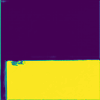
\includegraphics[interpolate=true,width=1.000000in,height=1.000000in]{unet_jaccard-img3.png}}%
\end{pgfscope}%
\begin{pgfscope}%
\definecolor{textcolor}{rgb}{0.000000,0.000000,0.000000}%
\pgfsetstrokecolor{textcolor}%
\pgfsetfillcolor{textcolor}%
\pgftext[x=3.564383in, y=3.502330in, left, base]{\color{textcolor}\rmfamily\fontsize{10.000000}{12.000000}\selectfont Binary }%
\end{pgfscope}%
\begin{pgfscope}%
\definecolor{textcolor}{rgb}{0.000000,0.000000,0.000000}%
\pgfsetstrokecolor{textcolor}%
\pgfsetfillcolor{textcolor}%
\pgftext[x=3.396559in, y=3.359583in, left, base]{\color{textcolor}\rmfamily\fontsize{10.000000}{12.000000}\selectfont  Crossentropy}%
\end{pgfscope}%
\begin{pgfscope}%
\pgfpathrectangle{\pgfqpoint{0.100000in}{1.191836in}}{\pgfqpoint{0.992578in}{0.992578in}}%
\pgfusepath{clip}%
\pgfsys@transformshift{0.100000in}{1.191836in}%
\pgftext[left,bottom]{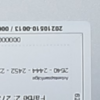
\includegraphics[interpolate=true,width=1.000000in,height=1.000000in]{unet_jaccard-img4.png}}%
\end{pgfscope}%
\begin{pgfscope}%
\pgfpathrectangle{\pgfqpoint{1.165625in}{1.191836in}}{\pgfqpoint{0.992578in}{0.992578in}}%
\pgfusepath{clip}%
\pgfsys@transformshift{1.165625in}{1.191836in}%
\pgftext[left,bottom]{
\includegraphics[interpolate=true,width=1.000000in,height=1.000000in]{unet_jaccard-img5.png}}%
\end{pgfscope}%
\begin{pgfscope}%
\pgfpathrectangle{\pgfqpoint{2.231250in}{1.191836in}}{\pgfqpoint{0.992578in}{0.992578in}}%
\pgfusepath{clip}%
\pgfsys@transformshift{2.231250in}{1.191836in}%
\pgftext[left,bottom]{
\includegraphics[interpolate=true,width=1.000000in,height=1.000000in]{unet_jaccard-img6.png}}%
\end{pgfscope}%
\begin{pgfscope}%
\pgfpathrectangle{\pgfqpoint{3.296875in}{1.191836in}}{\pgfqpoint{0.992578in}{0.992578in}}%
\pgfusepath{clip}%
\pgfsys@transformshift{3.296875in}{1.191836in}%
\pgftext[left,bottom]{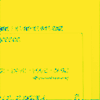
\includegraphics[interpolate=true,width=1.000000in,height=1.000000in]{unet_jaccard-img7.png}}%
\end{pgfscope}%
\begin{pgfscope}%
\pgfpathrectangle{\pgfqpoint{0.100000in}{0.100000in}}{\pgfqpoint{0.992578in}{0.992578in}}%
\pgfusepath{clip}%
\pgfsys@transformshift{0.100000in}{0.100000in}%
\pgftext[left,bottom]{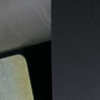
\includegraphics[interpolate=true,width=1.000000in,height=1.000000in]{unet_jaccard-img8.png}}%
\end{pgfscope}%
\begin{pgfscope}%
\pgfpathrectangle{\pgfqpoint{1.165625in}{0.100000in}}{\pgfqpoint{0.992578in}{0.992578in}}%
\pgfusepath{clip}%
\pgfsys@transformshift{1.165625in}{0.100000in}%
\pgftext[left,bottom]{
\includegraphics[interpolate=true,width=1.000000in,height=1.000000in]{unet_jaccard-img9.png}}%
\end{pgfscope}%
\begin{pgfscope}%
\pgfpathrectangle{\pgfqpoint{2.231250in}{0.100000in}}{\pgfqpoint{0.992578in}{0.992578in}}%
\pgfusepath{clip}%
\pgfsys@transformshift{2.231250in}{0.100000in}%
\pgftext[left,bottom]{
\includegraphics[interpolate=true,width=1.000000in,height=1.000000in]{unet_jaccard-img10.png}}%
\end{pgfscope}%
\begin{pgfscope}%
\pgfpathrectangle{\pgfqpoint{3.296875in}{0.100000in}}{\pgfqpoint{0.992578in}{0.992578in}}%
\pgfusepath{clip}%
\pgfsys@transformshift{3.296875in}{0.100000in}%
\pgftext[left,bottom]{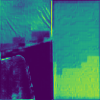
\includegraphics[interpolate=true,width=1.000000in,height=1.000000in]{unet_jaccard-img11.png}}%
\end{pgfscope}%
\end{pgfpicture}%
\makeatother%
\endgroup%

	\captionof{figure}[Metric of U-Net with complexity of 5 for multi-classification with different losses]{Metric of U-Net with complexity of 5 for multi-classification with different losses with training settings: Shift = False; Multi-Class = False; EarlyStopping = False; Epochs = 50; Complexity = 5; Image size = 256x256}
	\label{fig:loss_unet_jaccard}
	\vspace{5mm}
\end{minipage}
\begin{minipage}{\textwidth}
    \hspace{0.2cm}
    \inputpgf{Images/predictions/}{unet_jaccard.pgf}
	\captionof{figure}[Predictions of U-Net with complexity of 5 for multi-classification with different losses]{Predictions of U-Net with complexity of 5 for multi-classification with different losses with training settings: Shift = False; Multi-Class = False; EarlyStopping = False; Epochs = 50; Complexity = 5; Image size = 256x256}
	\label{fig:Preds_unet_jaccard}
	\vspace{5mm}
\end{minipage}



\subsection{Advanced Decoder}
From the results for the advanced decoder architecture one can see in \cref{fig:Decoder_nS_MCSC_Conv2DTranspose_50epochs} that the \verb|BatchNormalization| doesn't lead to a big improvement for the learning in case of single- and multi-classification. In the case of multi-classification the loss-curves with the \verb|BatchNormalization| lie even above the loss-curve without normalization.\\
However, it must be considered that only one \verb|BatchNormalization| was used (\cref{lst:Decoder-Transpose}) and not in a reasonable position. This could disturb the result and so the conclusions. It was repaired in the advanced decoder architecture in \cref{lst:Decoder-AdvancedDecoder} later on.\\
\begin{minipage}{\textwidth}
	%% Creator: Matplotlib, PGF backend
%%
%% To include the figure in your LaTeX document, write
%%   \input{<filename>.pgf}
%%
%% Make sure the required packages are loaded in your preamble
%%   \usepackage{pgf}
%%
%% Figures using additional raster images can only be included by \input if
%% they are in the same directory as the main LaTeX file. For loading figures
%% from other directories you can use the `import` package
%%   \usepackage{import}
%%
%% and then include the figures with
%%   \import{<path to file>}{<filename>.pgf}
%%
%% Matplotlib used the following preamble
%%
\begingroup%
\makeatletter%
\begin{pgfpicture}%
\pgfpathrectangle{\pgfpointorigin}{\pgfqpoint{4.598149in}{2.957916in}}%
\pgfusepath{use as bounding box, clip}%
\begin{pgfscope}%
\pgfsetbuttcap%
\pgfsetmiterjoin%
\definecolor{currentfill}{rgb}{1.000000,1.000000,1.000000}%
\pgfsetfillcolor{currentfill}%
\pgfsetlinewidth{0.000000pt}%
\definecolor{currentstroke}{rgb}{1.000000,1.000000,1.000000}%
\pgfsetstrokecolor{currentstroke}%
\pgfsetdash{}{0pt}%
\pgfpathmoveto{\pgfqpoint{0.000000in}{0.000000in}}%
\pgfpathlineto{\pgfqpoint{4.598149in}{0.000000in}}%
\pgfpathlineto{\pgfqpoint{4.598149in}{2.957916in}}%
\pgfpathlineto{\pgfqpoint{0.000000in}{2.957916in}}%
\pgfpathclose%
\pgfusepath{fill}%
\end{pgfscope}%
\begin{pgfscope}%
\pgfsetbuttcap%
\pgfsetmiterjoin%
\definecolor{currentfill}{rgb}{1.000000,1.000000,1.000000}%
\pgfsetfillcolor{currentfill}%
\pgfsetlinewidth{0.000000pt}%
\definecolor{currentstroke}{rgb}{0.000000,0.000000,0.000000}%
\pgfsetstrokecolor{currentstroke}%
\pgfsetstrokeopacity{0.000000}%
\pgfsetdash{}{0pt}%
\pgfpathmoveto{\pgfqpoint{0.623149in}{0.499691in}}%
\pgfpathlineto{\pgfqpoint{4.498149in}{0.499691in}}%
\pgfpathlineto{\pgfqpoint{4.498149in}{2.809691in}}%
\pgfpathlineto{\pgfqpoint{0.623149in}{2.809691in}}%
\pgfpathclose%
\pgfusepath{fill}%
\end{pgfscope}%
\begin{pgfscope}%
\pgfpathrectangle{\pgfqpoint{0.623149in}{0.499691in}}{\pgfqpoint{3.875000in}{2.310000in}}%
\pgfusepath{clip}%
\pgfsetrectcap%
\pgfsetroundjoin%
\pgfsetlinewidth{0.803000pt}%
\definecolor{currentstroke}{rgb}{0.690196,0.690196,0.690196}%
\pgfsetstrokecolor{currentstroke}%
\pgfsetdash{}{0pt}%
\pgfpathmoveto{\pgfqpoint{0.799285in}{0.499691in}}%
\pgfpathlineto{\pgfqpoint{0.799285in}{2.809691in}}%
\pgfusepath{stroke}%
\end{pgfscope}%
\begin{pgfscope}%
\pgfsetbuttcap%
\pgfsetroundjoin%
\definecolor{currentfill}{rgb}{0.000000,0.000000,0.000000}%
\pgfsetfillcolor{currentfill}%
\pgfsetlinewidth{0.803000pt}%
\definecolor{currentstroke}{rgb}{0.000000,0.000000,0.000000}%
\pgfsetstrokecolor{currentstroke}%
\pgfsetdash{}{0pt}%
\pgfsys@defobject{currentmarker}{\pgfqpoint{0.000000in}{-0.048611in}}{\pgfqpoint{0.000000in}{0.000000in}}{%
\pgfpathmoveto{\pgfqpoint{0.000000in}{0.000000in}}%
\pgfpathlineto{\pgfqpoint{0.000000in}{-0.048611in}}%
\pgfusepath{stroke,fill}%
}%
\begin{pgfscope}%
\pgfsys@transformshift{0.799285in}{0.499691in}%
\pgfsys@useobject{currentmarker}{}%
\end{pgfscope}%
\end{pgfscope}%
\begin{pgfscope}%
\definecolor{textcolor}{rgb}{0.000000,0.000000,0.000000}%
\pgfsetstrokecolor{textcolor}%
\pgfsetfillcolor{textcolor}%
\pgftext[x=0.799285in,y=0.402469in,,top]{\color{textcolor}\rmfamily\fontsize{10.000000}{12.000000}\selectfont \(\displaystyle {0}\)}%
\end{pgfscope}%
\begin{pgfscope}%
\pgfpathrectangle{\pgfqpoint{0.623149in}{0.499691in}}{\pgfqpoint{3.875000in}{2.310000in}}%
\pgfusepath{clip}%
\pgfsetrectcap%
\pgfsetroundjoin%
\pgfsetlinewidth{0.803000pt}%
\definecolor{currentstroke}{rgb}{0.690196,0.690196,0.690196}%
\pgfsetstrokecolor{currentstroke}%
\pgfsetdash{}{0pt}%
\pgfpathmoveto{\pgfqpoint{1.518209in}{0.499691in}}%
\pgfpathlineto{\pgfqpoint{1.518209in}{2.809691in}}%
\pgfusepath{stroke}%
\end{pgfscope}%
\begin{pgfscope}%
\pgfsetbuttcap%
\pgfsetroundjoin%
\definecolor{currentfill}{rgb}{0.000000,0.000000,0.000000}%
\pgfsetfillcolor{currentfill}%
\pgfsetlinewidth{0.803000pt}%
\definecolor{currentstroke}{rgb}{0.000000,0.000000,0.000000}%
\pgfsetstrokecolor{currentstroke}%
\pgfsetdash{}{0pt}%
\pgfsys@defobject{currentmarker}{\pgfqpoint{0.000000in}{-0.048611in}}{\pgfqpoint{0.000000in}{0.000000in}}{%
\pgfpathmoveto{\pgfqpoint{0.000000in}{0.000000in}}%
\pgfpathlineto{\pgfqpoint{0.000000in}{-0.048611in}}%
\pgfusepath{stroke,fill}%
}%
\begin{pgfscope}%
\pgfsys@transformshift{1.518209in}{0.499691in}%
\pgfsys@useobject{currentmarker}{}%
\end{pgfscope}%
\end{pgfscope}%
\begin{pgfscope}%
\definecolor{textcolor}{rgb}{0.000000,0.000000,0.000000}%
\pgfsetstrokecolor{textcolor}%
\pgfsetfillcolor{textcolor}%
\pgftext[x=1.518209in,y=0.402469in,,top]{\color{textcolor}\rmfamily\fontsize{10.000000}{12.000000}\selectfont \(\displaystyle {10}\)}%
\end{pgfscope}%
\begin{pgfscope}%
\pgfpathrectangle{\pgfqpoint{0.623149in}{0.499691in}}{\pgfqpoint{3.875000in}{2.310000in}}%
\pgfusepath{clip}%
\pgfsetrectcap%
\pgfsetroundjoin%
\pgfsetlinewidth{0.803000pt}%
\definecolor{currentstroke}{rgb}{0.690196,0.690196,0.690196}%
\pgfsetstrokecolor{currentstroke}%
\pgfsetdash{}{0pt}%
\pgfpathmoveto{\pgfqpoint{2.237133in}{0.499691in}}%
\pgfpathlineto{\pgfqpoint{2.237133in}{2.809691in}}%
\pgfusepath{stroke}%
\end{pgfscope}%
\begin{pgfscope}%
\pgfsetbuttcap%
\pgfsetroundjoin%
\definecolor{currentfill}{rgb}{0.000000,0.000000,0.000000}%
\pgfsetfillcolor{currentfill}%
\pgfsetlinewidth{0.803000pt}%
\definecolor{currentstroke}{rgb}{0.000000,0.000000,0.000000}%
\pgfsetstrokecolor{currentstroke}%
\pgfsetdash{}{0pt}%
\pgfsys@defobject{currentmarker}{\pgfqpoint{0.000000in}{-0.048611in}}{\pgfqpoint{0.000000in}{0.000000in}}{%
\pgfpathmoveto{\pgfqpoint{0.000000in}{0.000000in}}%
\pgfpathlineto{\pgfqpoint{0.000000in}{-0.048611in}}%
\pgfusepath{stroke,fill}%
}%
\begin{pgfscope}%
\pgfsys@transformshift{2.237133in}{0.499691in}%
\pgfsys@useobject{currentmarker}{}%
\end{pgfscope}%
\end{pgfscope}%
\begin{pgfscope}%
\definecolor{textcolor}{rgb}{0.000000,0.000000,0.000000}%
\pgfsetstrokecolor{textcolor}%
\pgfsetfillcolor{textcolor}%
\pgftext[x=2.237133in,y=0.402469in,,top]{\color{textcolor}\rmfamily\fontsize{10.000000}{12.000000}\selectfont \(\displaystyle {20}\)}%
\end{pgfscope}%
\begin{pgfscope}%
\pgfpathrectangle{\pgfqpoint{0.623149in}{0.499691in}}{\pgfqpoint{3.875000in}{2.310000in}}%
\pgfusepath{clip}%
\pgfsetrectcap%
\pgfsetroundjoin%
\pgfsetlinewidth{0.803000pt}%
\definecolor{currentstroke}{rgb}{0.690196,0.690196,0.690196}%
\pgfsetstrokecolor{currentstroke}%
\pgfsetdash{}{0pt}%
\pgfpathmoveto{\pgfqpoint{2.956057in}{0.499691in}}%
\pgfpathlineto{\pgfqpoint{2.956057in}{2.809691in}}%
\pgfusepath{stroke}%
\end{pgfscope}%
\begin{pgfscope}%
\pgfsetbuttcap%
\pgfsetroundjoin%
\definecolor{currentfill}{rgb}{0.000000,0.000000,0.000000}%
\pgfsetfillcolor{currentfill}%
\pgfsetlinewidth{0.803000pt}%
\definecolor{currentstroke}{rgb}{0.000000,0.000000,0.000000}%
\pgfsetstrokecolor{currentstroke}%
\pgfsetdash{}{0pt}%
\pgfsys@defobject{currentmarker}{\pgfqpoint{0.000000in}{-0.048611in}}{\pgfqpoint{0.000000in}{0.000000in}}{%
\pgfpathmoveto{\pgfqpoint{0.000000in}{0.000000in}}%
\pgfpathlineto{\pgfqpoint{0.000000in}{-0.048611in}}%
\pgfusepath{stroke,fill}%
}%
\begin{pgfscope}%
\pgfsys@transformshift{2.956057in}{0.499691in}%
\pgfsys@useobject{currentmarker}{}%
\end{pgfscope}%
\end{pgfscope}%
\begin{pgfscope}%
\definecolor{textcolor}{rgb}{0.000000,0.000000,0.000000}%
\pgfsetstrokecolor{textcolor}%
\pgfsetfillcolor{textcolor}%
\pgftext[x=2.956057in,y=0.402469in,,top]{\color{textcolor}\rmfamily\fontsize{10.000000}{12.000000}\selectfont \(\displaystyle {30}\)}%
\end{pgfscope}%
\begin{pgfscope}%
\pgfpathrectangle{\pgfqpoint{0.623149in}{0.499691in}}{\pgfqpoint{3.875000in}{2.310000in}}%
\pgfusepath{clip}%
\pgfsetrectcap%
\pgfsetroundjoin%
\pgfsetlinewidth{0.803000pt}%
\definecolor{currentstroke}{rgb}{0.690196,0.690196,0.690196}%
\pgfsetstrokecolor{currentstroke}%
\pgfsetdash{}{0pt}%
\pgfpathmoveto{\pgfqpoint{3.674981in}{0.499691in}}%
\pgfpathlineto{\pgfqpoint{3.674981in}{2.809691in}}%
\pgfusepath{stroke}%
\end{pgfscope}%
\begin{pgfscope}%
\pgfsetbuttcap%
\pgfsetroundjoin%
\definecolor{currentfill}{rgb}{0.000000,0.000000,0.000000}%
\pgfsetfillcolor{currentfill}%
\pgfsetlinewidth{0.803000pt}%
\definecolor{currentstroke}{rgb}{0.000000,0.000000,0.000000}%
\pgfsetstrokecolor{currentstroke}%
\pgfsetdash{}{0pt}%
\pgfsys@defobject{currentmarker}{\pgfqpoint{0.000000in}{-0.048611in}}{\pgfqpoint{0.000000in}{0.000000in}}{%
\pgfpathmoveto{\pgfqpoint{0.000000in}{0.000000in}}%
\pgfpathlineto{\pgfqpoint{0.000000in}{-0.048611in}}%
\pgfusepath{stroke,fill}%
}%
\begin{pgfscope}%
\pgfsys@transformshift{3.674981in}{0.499691in}%
\pgfsys@useobject{currentmarker}{}%
\end{pgfscope}%
\end{pgfscope}%
\begin{pgfscope}%
\definecolor{textcolor}{rgb}{0.000000,0.000000,0.000000}%
\pgfsetstrokecolor{textcolor}%
\pgfsetfillcolor{textcolor}%
\pgftext[x=3.674981in,y=0.402469in,,top]{\color{textcolor}\rmfamily\fontsize{10.000000}{12.000000}\selectfont \(\displaystyle {40}\)}%
\end{pgfscope}%
\begin{pgfscope}%
\pgfpathrectangle{\pgfqpoint{0.623149in}{0.499691in}}{\pgfqpoint{3.875000in}{2.310000in}}%
\pgfusepath{clip}%
\pgfsetrectcap%
\pgfsetroundjoin%
\pgfsetlinewidth{0.803000pt}%
\definecolor{currentstroke}{rgb}{0.690196,0.690196,0.690196}%
\pgfsetstrokecolor{currentstroke}%
\pgfsetdash{}{0pt}%
\pgfpathmoveto{\pgfqpoint{4.393905in}{0.499691in}}%
\pgfpathlineto{\pgfqpoint{4.393905in}{2.809691in}}%
\pgfusepath{stroke}%
\end{pgfscope}%
\begin{pgfscope}%
\pgfsetbuttcap%
\pgfsetroundjoin%
\definecolor{currentfill}{rgb}{0.000000,0.000000,0.000000}%
\pgfsetfillcolor{currentfill}%
\pgfsetlinewidth{0.803000pt}%
\definecolor{currentstroke}{rgb}{0.000000,0.000000,0.000000}%
\pgfsetstrokecolor{currentstroke}%
\pgfsetdash{}{0pt}%
\pgfsys@defobject{currentmarker}{\pgfqpoint{0.000000in}{-0.048611in}}{\pgfqpoint{0.000000in}{0.000000in}}{%
\pgfpathmoveto{\pgfqpoint{0.000000in}{0.000000in}}%
\pgfpathlineto{\pgfqpoint{0.000000in}{-0.048611in}}%
\pgfusepath{stroke,fill}%
}%
\begin{pgfscope}%
\pgfsys@transformshift{4.393905in}{0.499691in}%
\pgfsys@useobject{currentmarker}{}%
\end{pgfscope}%
\end{pgfscope}%
\begin{pgfscope}%
\definecolor{textcolor}{rgb}{0.000000,0.000000,0.000000}%
\pgfsetstrokecolor{textcolor}%
\pgfsetfillcolor{textcolor}%
\pgftext[x=4.393905in,y=0.402469in,,top]{\color{textcolor}\rmfamily\fontsize{10.000000}{12.000000}\selectfont \(\displaystyle {50}\)}%
\end{pgfscope}%
\begin{pgfscope}%
\definecolor{textcolor}{rgb}{0.000000,0.000000,0.000000}%
\pgfsetstrokecolor{textcolor}%
\pgfsetfillcolor{textcolor}%
\pgftext[x=2.560649in,y=0.223457in,,top]{\color{textcolor}\rmfamily\fontsize{10.000000}{12.000000}\selectfont Epochs}%
\end{pgfscope}%
\begin{pgfscope}%
\pgfpathrectangle{\pgfqpoint{0.623149in}{0.499691in}}{\pgfqpoint{3.875000in}{2.310000in}}%
\pgfusepath{clip}%
\pgfsetrectcap%
\pgfsetroundjoin%
\pgfsetlinewidth{0.803000pt}%
\definecolor{currentstroke}{rgb}{0.690196,0.690196,0.690196}%
\pgfsetstrokecolor{currentstroke}%
\pgfsetdash{}{0pt}%
\pgfpathmoveto{\pgfqpoint{0.623149in}{0.499691in}}%
\pgfpathlineto{\pgfqpoint{4.498149in}{0.499691in}}%
\pgfusepath{stroke}%
\end{pgfscope}%
\begin{pgfscope}%
\pgfsetbuttcap%
\pgfsetroundjoin%
\definecolor{currentfill}{rgb}{0.000000,0.000000,0.000000}%
\pgfsetfillcolor{currentfill}%
\pgfsetlinewidth{0.803000pt}%
\definecolor{currentstroke}{rgb}{0.000000,0.000000,0.000000}%
\pgfsetstrokecolor{currentstroke}%
\pgfsetdash{}{0pt}%
\pgfsys@defobject{currentmarker}{\pgfqpoint{-0.048611in}{0.000000in}}{\pgfqpoint{-0.000000in}{0.000000in}}{%
\pgfpathmoveto{\pgfqpoint{-0.000000in}{0.000000in}}%
\pgfpathlineto{\pgfqpoint{-0.048611in}{0.000000in}}%
\pgfusepath{stroke,fill}%
}%
\begin{pgfscope}%
\pgfsys@transformshift{0.623149in}{0.499691in}%
\pgfsys@useobject{currentmarker}{}%
\end{pgfscope}%
\end{pgfscope}%
\begin{pgfscope}%
\definecolor{textcolor}{rgb}{0.000000,0.000000,0.000000}%
\pgfsetstrokecolor{textcolor}%
\pgfsetfillcolor{textcolor}%
\pgftext[x=0.279012in, y=0.451466in, left, base]{\color{textcolor}\rmfamily\fontsize{10.000000}{12.000000}\selectfont \(\displaystyle {0.00}\)}%
\end{pgfscope}%
\begin{pgfscope}%
\pgfpathrectangle{\pgfqpoint{0.623149in}{0.499691in}}{\pgfqpoint{3.875000in}{2.310000in}}%
\pgfusepath{clip}%
\pgfsetrectcap%
\pgfsetroundjoin%
\pgfsetlinewidth{0.803000pt}%
\definecolor{currentstroke}{rgb}{0.690196,0.690196,0.690196}%
\pgfsetstrokecolor{currentstroke}%
\pgfsetdash{}{0pt}%
\pgfpathmoveto{\pgfqpoint{0.623149in}{0.884691in}}%
\pgfpathlineto{\pgfqpoint{4.498149in}{0.884691in}}%
\pgfusepath{stroke}%
\end{pgfscope}%
\begin{pgfscope}%
\pgfsetbuttcap%
\pgfsetroundjoin%
\definecolor{currentfill}{rgb}{0.000000,0.000000,0.000000}%
\pgfsetfillcolor{currentfill}%
\pgfsetlinewidth{0.803000pt}%
\definecolor{currentstroke}{rgb}{0.000000,0.000000,0.000000}%
\pgfsetstrokecolor{currentstroke}%
\pgfsetdash{}{0pt}%
\pgfsys@defobject{currentmarker}{\pgfqpoint{-0.048611in}{0.000000in}}{\pgfqpoint{-0.000000in}{0.000000in}}{%
\pgfpathmoveto{\pgfqpoint{-0.000000in}{0.000000in}}%
\pgfpathlineto{\pgfqpoint{-0.048611in}{0.000000in}}%
\pgfusepath{stroke,fill}%
}%
\begin{pgfscope}%
\pgfsys@transformshift{0.623149in}{0.884691in}%
\pgfsys@useobject{currentmarker}{}%
\end{pgfscope}%
\end{pgfscope}%
\begin{pgfscope}%
\definecolor{textcolor}{rgb}{0.000000,0.000000,0.000000}%
\pgfsetstrokecolor{textcolor}%
\pgfsetfillcolor{textcolor}%
\pgftext[x=0.279012in, y=0.836466in, left, base]{\color{textcolor}\rmfamily\fontsize{10.000000}{12.000000}\selectfont \(\displaystyle {0.05}\)}%
\end{pgfscope}%
\begin{pgfscope}%
\pgfpathrectangle{\pgfqpoint{0.623149in}{0.499691in}}{\pgfqpoint{3.875000in}{2.310000in}}%
\pgfusepath{clip}%
\pgfsetrectcap%
\pgfsetroundjoin%
\pgfsetlinewidth{0.803000pt}%
\definecolor{currentstroke}{rgb}{0.690196,0.690196,0.690196}%
\pgfsetstrokecolor{currentstroke}%
\pgfsetdash{}{0pt}%
\pgfpathmoveto{\pgfqpoint{0.623149in}{1.269691in}}%
\pgfpathlineto{\pgfqpoint{4.498149in}{1.269691in}}%
\pgfusepath{stroke}%
\end{pgfscope}%
\begin{pgfscope}%
\pgfsetbuttcap%
\pgfsetroundjoin%
\definecolor{currentfill}{rgb}{0.000000,0.000000,0.000000}%
\pgfsetfillcolor{currentfill}%
\pgfsetlinewidth{0.803000pt}%
\definecolor{currentstroke}{rgb}{0.000000,0.000000,0.000000}%
\pgfsetstrokecolor{currentstroke}%
\pgfsetdash{}{0pt}%
\pgfsys@defobject{currentmarker}{\pgfqpoint{-0.048611in}{0.000000in}}{\pgfqpoint{-0.000000in}{0.000000in}}{%
\pgfpathmoveto{\pgfqpoint{-0.000000in}{0.000000in}}%
\pgfpathlineto{\pgfqpoint{-0.048611in}{0.000000in}}%
\pgfusepath{stroke,fill}%
}%
\begin{pgfscope}%
\pgfsys@transformshift{0.623149in}{1.269691in}%
\pgfsys@useobject{currentmarker}{}%
\end{pgfscope}%
\end{pgfscope}%
\begin{pgfscope}%
\definecolor{textcolor}{rgb}{0.000000,0.000000,0.000000}%
\pgfsetstrokecolor{textcolor}%
\pgfsetfillcolor{textcolor}%
\pgftext[x=0.279012in, y=1.221466in, left, base]{\color{textcolor}\rmfamily\fontsize{10.000000}{12.000000}\selectfont \(\displaystyle {0.10}\)}%
\end{pgfscope}%
\begin{pgfscope}%
\pgfpathrectangle{\pgfqpoint{0.623149in}{0.499691in}}{\pgfqpoint{3.875000in}{2.310000in}}%
\pgfusepath{clip}%
\pgfsetrectcap%
\pgfsetroundjoin%
\pgfsetlinewidth{0.803000pt}%
\definecolor{currentstroke}{rgb}{0.690196,0.690196,0.690196}%
\pgfsetstrokecolor{currentstroke}%
\pgfsetdash{}{0pt}%
\pgfpathmoveto{\pgfqpoint{0.623149in}{1.654691in}}%
\pgfpathlineto{\pgfqpoint{4.498149in}{1.654691in}}%
\pgfusepath{stroke}%
\end{pgfscope}%
\begin{pgfscope}%
\pgfsetbuttcap%
\pgfsetroundjoin%
\definecolor{currentfill}{rgb}{0.000000,0.000000,0.000000}%
\pgfsetfillcolor{currentfill}%
\pgfsetlinewidth{0.803000pt}%
\definecolor{currentstroke}{rgb}{0.000000,0.000000,0.000000}%
\pgfsetstrokecolor{currentstroke}%
\pgfsetdash{}{0pt}%
\pgfsys@defobject{currentmarker}{\pgfqpoint{-0.048611in}{0.000000in}}{\pgfqpoint{-0.000000in}{0.000000in}}{%
\pgfpathmoveto{\pgfqpoint{-0.000000in}{0.000000in}}%
\pgfpathlineto{\pgfqpoint{-0.048611in}{0.000000in}}%
\pgfusepath{stroke,fill}%
}%
\begin{pgfscope}%
\pgfsys@transformshift{0.623149in}{1.654691in}%
\pgfsys@useobject{currentmarker}{}%
\end{pgfscope}%
\end{pgfscope}%
\begin{pgfscope}%
\definecolor{textcolor}{rgb}{0.000000,0.000000,0.000000}%
\pgfsetstrokecolor{textcolor}%
\pgfsetfillcolor{textcolor}%
\pgftext[x=0.279012in, y=1.606466in, left, base]{\color{textcolor}\rmfamily\fontsize{10.000000}{12.000000}\selectfont \(\displaystyle {0.15}\)}%
\end{pgfscope}%
\begin{pgfscope}%
\pgfpathrectangle{\pgfqpoint{0.623149in}{0.499691in}}{\pgfqpoint{3.875000in}{2.310000in}}%
\pgfusepath{clip}%
\pgfsetrectcap%
\pgfsetroundjoin%
\pgfsetlinewidth{0.803000pt}%
\definecolor{currentstroke}{rgb}{0.690196,0.690196,0.690196}%
\pgfsetstrokecolor{currentstroke}%
\pgfsetdash{}{0pt}%
\pgfpathmoveto{\pgfqpoint{0.623149in}{2.039691in}}%
\pgfpathlineto{\pgfqpoint{4.498149in}{2.039691in}}%
\pgfusepath{stroke}%
\end{pgfscope}%
\begin{pgfscope}%
\pgfsetbuttcap%
\pgfsetroundjoin%
\definecolor{currentfill}{rgb}{0.000000,0.000000,0.000000}%
\pgfsetfillcolor{currentfill}%
\pgfsetlinewidth{0.803000pt}%
\definecolor{currentstroke}{rgb}{0.000000,0.000000,0.000000}%
\pgfsetstrokecolor{currentstroke}%
\pgfsetdash{}{0pt}%
\pgfsys@defobject{currentmarker}{\pgfqpoint{-0.048611in}{0.000000in}}{\pgfqpoint{-0.000000in}{0.000000in}}{%
\pgfpathmoveto{\pgfqpoint{-0.000000in}{0.000000in}}%
\pgfpathlineto{\pgfqpoint{-0.048611in}{0.000000in}}%
\pgfusepath{stroke,fill}%
}%
\begin{pgfscope}%
\pgfsys@transformshift{0.623149in}{2.039691in}%
\pgfsys@useobject{currentmarker}{}%
\end{pgfscope}%
\end{pgfscope}%
\begin{pgfscope}%
\definecolor{textcolor}{rgb}{0.000000,0.000000,0.000000}%
\pgfsetstrokecolor{textcolor}%
\pgfsetfillcolor{textcolor}%
\pgftext[x=0.279012in, y=1.991466in, left, base]{\color{textcolor}\rmfamily\fontsize{10.000000}{12.000000}\selectfont \(\displaystyle {0.20}\)}%
\end{pgfscope}%
\begin{pgfscope}%
\pgfpathrectangle{\pgfqpoint{0.623149in}{0.499691in}}{\pgfqpoint{3.875000in}{2.310000in}}%
\pgfusepath{clip}%
\pgfsetrectcap%
\pgfsetroundjoin%
\pgfsetlinewidth{0.803000pt}%
\definecolor{currentstroke}{rgb}{0.690196,0.690196,0.690196}%
\pgfsetstrokecolor{currentstroke}%
\pgfsetdash{}{0pt}%
\pgfpathmoveto{\pgfqpoint{0.623149in}{2.424691in}}%
\pgfpathlineto{\pgfqpoint{4.498149in}{2.424691in}}%
\pgfusepath{stroke}%
\end{pgfscope}%
\begin{pgfscope}%
\pgfsetbuttcap%
\pgfsetroundjoin%
\definecolor{currentfill}{rgb}{0.000000,0.000000,0.000000}%
\pgfsetfillcolor{currentfill}%
\pgfsetlinewidth{0.803000pt}%
\definecolor{currentstroke}{rgb}{0.000000,0.000000,0.000000}%
\pgfsetstrokecolor{currentstroke}%
\pgfsetdash{}{0pt}%
\pgfsys@defobject{currentmarker}{\pgfqpoint{-0.048611in}{0.000000in}}{\pgfqpoint{-0.000000in}{0.000000in}}{%
\pgfpathmoveto{\pgfqpoint{-0.000000in}{0.000000in}}%
\pgfpathlineto{\pgfqpoint{-0.048611in}{0.000000in}}%
\pgfusepath{stroke,fill}%
}%
\begin{pgfscope}%
\pgfsys@transformshift{0.623149in}{2.424691in}%
\pgfsys@useobject{currentmarker}{}%
\end{pgfscope}%
\end{pgfscope}%
\begin{pgfscope}%
\definecolor{textcolor}{rgb}{0.000000,0.000000,0.000000}%
\pgfsetstrokecolor{textcolor}%
\pgfsetfillcolor{textcolor}%
\pgftext[x=0.279012in, y=2.376466in, left, base]{\color{textcolor}\rmfamily\fontsize{10.000000}{12.000000}\selectfont \(\displaystyle {0.25}\)}%
\end{pgfscope}%
\begin{pgfscope}%
\pgfpathrectangle{\pgfqpoint{0.623149in}{0.499691in}}{\pgfqpoint{3.875000in}{2.310000in}}%
\pgfusepath{clip}%
\pgfsetrectcap%
\pgfsetroundjoin%
\pgfsetlinewidth{0.803000pt}%
\definecolor{currentstroke}{rgb}{0.690196,0.690196,0.690196}%
\pgfsetstrokecolor{currentstroke}%
\pgfsetdash{}{0pt}%
\pgfpathmoveto{\pgfqpoint{0.623149in}{2.809691in}}%
\pgfpathlineto{\pgfqpoint{4.498149in}{2.809691in}}%
\pgfusepath{stroke}%
\end{pgfscope}%
\begin{pgfscope}%
\pgfsetbuttcap%
\pgfsetroundjoin%
\definecolor{currentfill}{rgb}{0.000000,0.000000,0.000000}%
\pgfsetfillcolor{currentfill}%
\pgfsetlinewidth{0.803000pt}%
\definecolor{currentstroke}{rgb}{0.000000,0.000000,0.000000}%
\pgfsetstrokecolor{currentstroke}%
\pgfsetdash{}{0pt}%
\pgfsys@defobject{currentmarker}{\pgfqpoint{-0.048611in}{0.000000in}}{\pgfqpoint{-0.000000in}{0.000000in}}{%
\pgfpathmoveto{\pgfqpoint{-0.000000in}{0.000000in}}%
\pgfpathlineto{\pgfqpoint{-0.048611in}{0.000000in}}%
\pgfusepath{stroke,fill}%
}%
\begin{pgfscope}%
\pgfsys@transformshift{0.623149in}{2.809691in}%
\pgfsys@useobject{currentmarker}{}%
\end{pgfscope}%
\end{pgfscope}%
\begin{pgfscope}%
\definecolor{textcolor}{rgb}{0.000000,0.000000,0.000000}%
\pgfsetstrokecolor{textcolor}%
\pgfsetfillcolor{textcolor}%
\pgftext[x=0.279012in, y=2.761466in, left, base]{\color{textcolor}\rmfamily\fontsize{10.000000}{12.000000}\selectfont \(\displaystyle {0.30}\)}%
\end{pgfscope}%
\begin{pgfscope}%
\definecolor{textcolor}{rgb}{0.000000,0.000000,0.000000}%
\pgfsetstrokecolor{textcolor}%
\pgfsetfillcolor{textcolor}%
\pgftext[x=0.223457in,y=1.654691in,,bottom,rotate=90.000000]{\color{textcolor}\rmfamily\fontsize{10.000000}{12.000000}\selectfont Loss}%
\end{pgfscope}%
\begin{pgfscope}%
\pgfpathrectangle{\pgfqpoint{0.623149in}{0.499691in}}{\pgfqpoint{3.875000in}{2.310000in}}%
\pgfusepath{clip}%
\pgfsetrectcap%
\pgfsetroundjoin%
\pgfsetlinewidth{1.003750pt}%
\definecolor{currentstroke}{rgb}{0.274510,0.509804,0.705882}%
\pgfsetstrokecolor{currentstroke}%
\pgfsetdash{}{0pt}%
\pgfpathmoveto{\pgfqpoint{1.032977in}{2.819691in}}%
\pgfpathlineto{\pgfqpoint{1.086855in}{2.117234in}}%
\pgfpathlineto{\pgfqpoint{1.158747in}{1.829014in}}%
\pgfpathlineto{\pgfqpoint{1.230639in}{1.695974in}}%
\pgfpathlineto{\pgfqpoint{1.302532in}{1.651639in}}%
\pgfpathlineto{\pgfqpoint{1.374424in}{1.538997in}}%
\pgfpathlineto{\pgfqpoint{1.446317in}{1.133213in}}%
\pgfpathlineto{\pgfqpoint{1.518209in}{1.324236in}}%
\pgfpathlineto{\pgfqpoint{1.590101in}{1.256667in}}%
\pgfpathlineto{\pgfqpoint{1.661994in}{1.422936in}}%
\pgfpathlineto{\pgfqpoint{1.733886in}{1.491433in}}%
\pgfpathlineto{\pgfqpoint{1.805779in}{1.511316in}}%
\pgfpathlineto{\pgfqpoint{1.877671in}{1.381683in}}%
\pgfpathlineto{\pgfqpoint{1.949563in}{1.088042in}}%
\pgfpathlineto{\pgfqpoint{2.021456in}{1.095632in}}%
\pgfpathlineto{\pgfqpoint{2.093348in}{1.139505in}}%
\pgfpathlineto{\pgfqpoint{2.165241in}{0.980083in}}%
\pgfpathlineto{\pgfqpoint{2.237133in}{1.333564in}}%
\pgfpathlineto{\pgfqpoint{2.309025in}{1.255904in}}%
\pgfpathlineto{\pgfqpoint{2.380918in}{1.027274in}}%
\pgfpathlineto{\pgfqpoint{2.452810in}{1.061527in}}%
\pgfpathlineto{\pgfqpoint{2.524703in}{1.411477in}}%
\pgfpathlineto{\pgfqpoint{2.596595in}{0.913600in}}%
\pgfpathlineto{\pgfqpoint{2.668487in}{0.744847in}}%
\pgfpathlineto{\pgfqpoint{2.740380in}{0.762295in}}%
\pgfpathlineto{\pgfqpoint{2.812272in}{1.026061in}}%
\pgfpathlineto{\pgfqpoint{2.884165in}{0.796351in}}%
\pgfpathlineto{\pgfqpoint{2.956057in}{0.848688in}}%
\pgfpathlineto{\pgfqpoint{3.027949in}{1.316799in}}%
\pgfpathlineto{\pgfqpoint{3.099842in}{1.135513in}}%
\pgfpathlineto{\pgfqpoint{3.171734in}{1.166332in}}%
\pgfpathlineto{\pgfqpoint{3.243626in}{1.127385in}}%
\pgfpathlineto{\pgfqpoint{3.315519in}{1.143876in}}%
\pgfpathlineto{\pgfqpoint{3.387411in}{1.102052in}}%
\pgfpathlineto{\pgfqpoint{3.459304in}{1.103049in}}%
\pgfpathlineto{\pgfqpoint{3.531196in}{1.006331in}}%
\pgfpathlineto{\pgfqpoint{3.603088in}{1.060690in}}%
\pgfpathlineto{\pgfqpoint{3.674981in}{0.943776in}}%
\pgfpathlineto{\pgfqpoint{3.746873in}{1.032322in}}%
\pgfpathlineto{\pgfqpoint{3.818766in}{1.253042in}}%
\pgfpathlineto{\pgfqpoint{3.890658in}{0.967382in}}%
\pgfpathlineto{\pgfqpoint{3.962550in}{0.913109in}}%
\pgfpathlineto{\pgfqpoint{4.034443in}{0.845096in}}%
\pgfpathlineto{\pgfqpoint{4.106335in}{0.799413in}}%
\pgfpathlineto{\pgfqpoint{4.178228in}{1.091069in}}%
\pgfpathlineto{\pgfqpoint{4.250120in}{0.979278in}}%
\pgfpathlineto{\pgfqpoint{4.322012in}{0.883705in}}%
\pgfusepath{stroke}%
\end{pgfscope}%
\begin{pgfscope}%
\pgfpathrectangle{\pgfqpoint{0.623149in}{0.499691in}}{\pgfqpoint{3.875000in}{2.310000in}}%
\pgfusepath{clip}%
\pgfsetbuttcap%
\pgfsetroundjoin%
\pgfsetlinewidth{1.003750pt}%
\definecolor{currentstroke}{rgb}{0.274510,0.509804,0.705882}%
\pgfsetstrokecolor{currentstroke}%
\pgfsetdash{{1.000000pt}{1.650000pt}}{0.000000pt}%
\pgfpathmoveto{\pgfqpoint{0.942382in}{2.819691in}}%
\pgfpathlineto{\pgfqpoint{0.943070in}{2.805157in}}%
\pgfpathlineto{\pgfqpoint{1.014962in}{1.919341in}}%
\pgfpathlineto{\pgfqpoint{1.086855in}{1.799262in}}%
\pgfpathlineto{\pgfqpoint{1.158747in}{1.534215in}}%
\pgfpathlineto{\pgfqpoint{1.230639in}{1.430284in}}%
\pgfpathlineto{\pgfqpoint{1.302532in}{1.249595in}}%
\pgfpathlineto{\pgfqpoint{1.374424in}{1.191925in}}%
\pgfpathlineto{\pgfqpoint{1.446317in}{1.062039in}}%
\pgfpathlineto{\pgfqpoint{1.518209in}{1.088165in}}%
\pgfpathlineto{\pgfqpoint{1.590101in}{1.036090in}}%
\pgfpathlineto{\pgfqpoint{1.661994in}{1.048316in}}%
\pgfpathlineto{\pgfqpoint{1.733886in}{1.082565in}}%
\pgfpathlineto{\pgfqpoint{1.805779in}{1.017945in}}%
\pgfpathlineto{\pgfqpoint{1.877671in}{1.078640in}}%
\pgfpathlineto{\pgfqpoint{1.949563in}{0.998100in}}%
\pgfpathlineto{\pgfqpoint{2.021456in}{0.942334in}}%
\pgfpathlineto{\pgfqpoint{2.093348in}{0.974139in}}%
\pgfpathlineto{\pgfqpoint{2.165241in}{0.910233in}}%
\pgfpathlineto{\pgfqpoint{2.237133in}{1.077361in}}%
\pgfpathlineto{\pgfqpoint{2.309025in}{0.979065in}}%
\pgfpathlineto{\pgfqpoint{2.380918in}{0.999541in}}%
\pgfpathlineto{\pgfqpoint{2.452810in}{0.925310in}}%
\pgfpathlineto{\pgfqpoint{2.524703in}{1.051785in}}%
\pgfpathlineto{\pgfqpoint{2.596595in}{0.872627in}}%
\pgfpathlineto{\pgfqpoint{2.668487in}{0.863319in}}%
\pgfpathlineto{\pgfqpoint{2.740380in}{0.858797in}}%
\pgfpathlineto{\pgfqpoint{2.812272in}{0.882857in}}%
\pgfpathlineto{\pgfqpoint{2.884165in}{0.872994in}}%
\pgfpathlineto{\pgfqpoint{2.956057in}{0.843737in}}%
\pgfpathlineto{\pgfqpoint{3.027949in}{1.012159in}}%
\pgfpathlineto{\pgfqpoint{3.099842in}{0.959476in}}%
\pgfpathlineto{\pgfqpoint{3.171734in}{0.911242in}}%
\pgfpathlineto{\pgfqpoint{3.243626in}{0.880526in}}%
\pgfpathlineto{\pgfqpoint{3.315519in}{0.947119in}}%
\pgfpathlineto{\pgfqpoint{3.387411in}{0.834404in}}%
\pgfpathlineto{\pgfqpoint{3.459304in}{0.930286in}}%
\pgfpathlineto{\pgfqpoint{3.531196in}{0.829238in}}%
\pgfpathlineto{\pgfqpoint{3.603088in}{0.820219in}}%
\pgfpathlineto{\pgfqpoint{3.674981in}{0.823977in}}%
\pgfpathlineto{\pgfqpoint{3.746873in}{0.854919in}}%
\pgfpathlineto{\pgfqpoint{3.818766in}{1.069982in}}%
\pgfpathlineto{\pgfqpoint{3.890658in}{0.859743in}}%
\pgfpathlineto{\pgfqpoint{3.962550in}{0.846403in}}%
\pgfpathlineto{\pgfqpoint{4.034443in}{0.795204in}}%
\pgfpathlineto{\pgfqpoint{4.106335in}{0.776409in}}%
\pgfpathlineto{\pgfqpoint{4.178228in}{0.888561in}}%
\pgfpathlineto{\pgfqpoint{4.250120in}{0.767741in}}%
\pgfpathlineto{\pgfqpoint{4.322012in}{0.786562in}}%
\pgfusepath{stroke}%
\end{pgfscope}%
\begin{pgfscope}%
\pgfpathrectangle{\pgfqpoint{0.623149in}{0.499691in}}{\pgfqpoint{3.875000in}{2.310000in}}%
\pgfusepath{clip}%
\pgfsetrectcap%
\pgfsetroundjoin%
\pgfsetlinewidth{1.003750pt}%
\definecolor{currentstroke}{rgb}{1.000000,0.498039,0.313725}%
\pgfsetstrokecolor{currentstroke}%
\pgfsetdash{}{0pt}%
\pgfpathmoveto{\pgfqpoint{1.060965in}{2.819691in}}%
\pgfpathlineto{\pgfqpoint{1.086855in}{2.574616in}}%
\pgfpathlineto{\pgfqpoint{1.158747in}{2.155430in}}%
\pgfpathlineto{\pgfqpoint{1.230639in}{2.068510in}}%
\pgfpathlineto{\pgfqpoint{1.302532in}{1.986285in}}%
\pgfpathlineto{\pgfqpoint{1.374424in}{2.165709in}}%
\pgfpathlineto{\pgfqpoint{1.446317in}{1.611177in}}%
\pgfpathlineto{\pgfqpoint{1.518209in}{1.771210in}}%
\pgfpathlineto{\pgfqpoint{1.590101in}{1.701527in}}%
\pgfpathlineto{\pgfqpoint{1.661994in}{1.856719in}}%
\pgfpathlineto{\pgfqpoint{1.733886in}{2.297457in}}%
\pgfpathlineto{\pgfqpoint{1.805779in}{1.908652in}}%
\pgfpathlineto{\pgfqpoint{1.877671in}{1.858871in}}%
\pgfpathlineto{\pgfqpoint{1.949563in}{1.604538in}}%
\pgfpathlineto{\pgfqpoint{2.021456in}{1.831290in}}%
\pgfpathlineto{\pgfqpoint{2.093348in}{1.471651in}}%
\pgfpathlineto{\pgfqpoint{2.165241in}{1.247503in}}%
\pgfpathlineto{\pgfqpoint{2.237133in}{1.584788in}}%
\pgfpathlineto{\pgfqpoint{2.309025in}{1.430475in}}%
\pgfpathlineto{\pgfqpoint{2.380918in}{1.228283in}}%
\pgfpathlineto{\pgfqpoint{2.452810in}{1.244404in}}%
\pgfpathlineto{\pgfqpoint{2.524703in}{1.595611in}}%
\pgfpathlineto{\pgfqpoint{2.596595in}{1.134187in}}%
\pgfpathlineto{\pgfqpoint{2.668487in}{1.058603in}}%
\pgfpathlineto{\pgfqpoint{2.740380in}{0.981491in}}%
\pgfpathlineto{\pgfqpoint{2.812272in}{1.083390in}}%
\pgfpathlineto{\pgfqpoint{2.884165in}{0.944417in}}%
\pgfpathlineto{\pgfqpoint{2.956057in}{0.926877in}}%
\pgfpathlineto{\pgfqpoint{3.027949in}{1.450423in}}%
\pgfpathlineto{\pgfqpoint{3.099842in}{1.246746in}}%
\pgfpathlineto{\pgfqpoint{3.171734in}{1.337621in}}%
\pgfpathlineto{\pgfqpoint{3.243626in}{1.165003in}}%
\pgfpathlineto{\pgfqpoint{3.315519in}{1.225334in}}%
\pgfpathlineto{\pgfqpoint{3.387411in}{1.212882in}}%
\pgfpathlineto{\pgfqpoint{3.459304in}{1.081917in}}%
\pgfpathlineto{\pgfqpoint{3.531196in}{1.096170in}}%
\pgfpathlineto{\pgfqpoint{3.603088in}{1.118950in}}%
\pgfpathlineto{\pgfqpoint{3.674981in}{1.084013in}}%
\pgfpathlineto{\pgfqpoint{3.746873in}{1.072344in}}%
\pgfpathlineto{\pgfqpoint{3.818766in}{1.270904in}}%
\pgfpathlineto{\pgfqpoint{3.890658in}{0.947034in}}%
\pgfpathlineto{\pgfqpoint{3.962550in}{1.088585in}}%
\pgfpathlineto{\pgfqpoint{4.034443in}{0.931196in}}%
\pgfpathlineto{\pgfqpoint{4.106335in}{0.989333in}}%
\pgfpathlineto{\pgfqpoint{4.178228in}{1.393421in}}%
\pgfpathlineto{\pgfqpoint{4.250120in}{1.058529in}}%
\pgfpathlineto{\pgfqpoint{4.322012in}{0.969795in}}%
\pgfusepath{stroke}%
\end{pgfscope}%
\begin{pgfscope}%
\pgfpathrectangle{\pgfqpoint{0.623149in}{0.499691in}}{\pgfqpoint{3.875000in}{2.310000in}}%
\pgfusepath{clip}%
\pgfsetbuttcap%
\pgfsetroundjoin%
\pgfsetlinewidth{1.003750pt}%
\definecolor{currentstroke}{rgb}{1.000000,0.498039,0.313725}%
\pgfsetstrokecolor{currentstroke}%
\pgfsetdash{{1.000000pt}{1.650000pt}}{0.000000pt}%
\pgfpathmoveto{\pgfqpoint{1.103858in}{2.819691in}}%
\pgfpathlineto{\pgfqpoint{1.158747in}{2.314266in}}%
\pgfpathlineto{\pgfqpoint{1.230639in}{2.022140in}}%
\pgfpathlineto{\pgfqpoint{1.302532in}{1.878370in}}%
\pgfpathlineto{\pgfqpoint{1.374424in}{1.924854in}}%
\pgfpathlineto{\pgfqpoint{1.446317in}{1.792855in}}%
\pgfpathlineto{\pgfqpoint{1.518209in}{1.548321in}}%
\pgfpathlineto{\pgfqpoint{1.590101in}{1.397436in}}%
\pgfpathlineto{\pgfqpoint{1.661994in}{1.470636in}}%
\pgfpathlineto{\pgfqpoint{1.733886in}{1.585251in}}%
\pgfpathlineto{\pgfqpoint{1.805779in}{1.487088in}}%
\pgfpathlineto{\pgfqpoint{1.877671in}{1.623656in}}%
\pgfpathlineto{\pgfqpoint{1.949563in}{1.559863in}}%
\pgfpathlineto{\pgfqpoint{2.021456in}{1.163373in}}%
\pgfpathlineto{\pgfqpoint{2.093348in}{1.223652in}}%
\pgfpathlineto{\pgfqpoint{2.165241in}{1.232561in}}%
\pgfpathlineto{\pgfqpoint{2.237133in}{1.418325in}}%
\pgfpathlineto{\pgfqpoint{2.309025in}{1.114475in}}%
\pgfpathlineto{\pgfqpoint{2.380918in}{1.143367in}}%
\pgfpathlineto{\pgfqpoint{2.452810in}{0.957567in}}%
\pgfpathlineto{\pgfqpoint{2.524703in}{1.059037in}}%
\pgfpathlineto{\pgfqpoint{2.596595in}{0.993796in}}%
\pgfpathlineto{\pgfqpoint{2.668487in}{0.948671in}}%
\pgfpathlineto{\pgfqpoint{2.740380in}{0.928671in}}%
\pgfpathlineto{\pgfqpoint{2.812272in}{0.976180in}}%
\pgfpathlineto{\pgfqpoint{2.884165in}{0.933324in}}%
\pgfpathlineto{\pgfqpoint{2.956057in}{0.923354in}}%
\pgfpathlineto{\pgfqpoint{3.027949in}{1.429976in}}%
\pgfpathlineto{\pgfqpoint{3.099842in}{0.931599in}}%
\pgfpathlineto{\pgfqpoint{3.171734in}{0.903583in}}%
\pgfpathlineto{\pgfqpoint{3.243626in}{0.907351in}}%
\pgfpathlineto{\pgfqpoint{3.315519in}{0.874215in}}%
\pgfpathlineto{\pgfqpoint{3.387411in}{0.877346in}}%
\pgfpathlineto{\pgfqpoint{3.459304in}{0.860642in}}%
\pgfpathlineto{\pgfqpoint{3.531196in}{0.838485in}}%
\pgfpathlineto{\pgfqpoint{3.603088in}{0.845440in}}%
\pgfpathlineto{\pgfqpoint{3.674981in}{0.876139in}}%
\pgfpathlineto{\pgfqpoint{3.746873in}{0.878382in}}%
\pgfpathlineto{\pgfqpoint{3.818766in}{0.853719in}}%
\pgfpathlineto{\pgfqpoint{3.890658in}{0.871512in}}%
\pgfpathlineto{\pgfqpoint{3.962550in}{0.895284in}}%
\pgfpathlineto{\pgfqpoint{4.034443in}{0.811503in}}%
\pgfpathlineto{\pgfqpoint{4.106335in}{0.816831in}}%
\pgfpathlineto{\pgfqpoint{4.178228in}{0.879002in}}%
\pgfpathlineto{\pgfqpoint{4.250120in}{0.942757in}}%
\pgfpathlineto{\pgfqpoint{4.322012in}{0.805144in}}%
\pgfusepath{stroke}%
\end{pgfscope}%
\begin{pgfscope}%
\pgfpathrectangle{\pgfqpoint{0.623149in}{0.499691in}}{\pgfqpoint{3.875000in}{2.310000in}}%
\pgfusepath{clip}%
\pgfsetrectcap%
\pgfsetroundjoin%
\pgfsetlinewidth{1.003750pt}%
\definecolor{currentstroke}{rgb}{0.172549,0.627451,0.172549}%
\pgfsetstrokecolor{currentstroke}%
\pgfsetdash{}{0pt}%
\pgfpathmoveto{\pgfqpoint{0.910777in}{2.819691in}}%
\pgfpathlineto{\pgfqpoint{0.943070in}{2.367356in}}%
\pgfpathlineto{\pgfqpoint{1.014962in}{2.010192in}}%
\pgfpathlineto{\pgfqpoint{1.086855in}{1.853734in}}%
\pgfpathlineto{\pgfqpoint{1.158747in}{1.418603in}}%
\pgfpathlineto{\pgfqpoint{1.230639in}{1.322591in}}%
\pgfpathlineto{\pgfqpoint{1.302532in}{1.460519in}}%
\pgfpathlineto{\pgfqpoint{1.374424in}{1.467422in}}%
\pgfpathlineto{\pgfqpoint{1.446317in}{1.058449in}}%
\pgfpathlineto{\pgfqpoint{1.518209in}{1.226838in}}%
\pgfpathlineto{\pgfqpoint{1.590101in}{1.183918in}}%
\pgfpathlineto{\pgfqpoint{1.661994in}{1.296164in}}%
\pgfpathlineto{\pgfqpoint{1.733886in}{1.489578in}}%
\pgfpathlineto{\pgfqpoint{1.805779in}{1.356339in}}%
\pgfpathlineto{\pgfqpoint{1.877671in}{1.271537in}}%
\pgfpathlineto{\pgfqpoint{1.949563in}{0.976728in}}%
\pgfpathlineto{\pgfqpoint{2.021456in}{1.127274in}}%
\pgfpathlineto{\pgfqpoint{2.093348in}{1.028006in}}%
\pgfpathlineto{\pgfqpoint{2.165241in}{0.915437in}}%
\pgfpathlineto{\pgfqpoint{2.237133in}{1.254327in}}%
\pgfpathlineto{\pgfqpoint{2.309025in}{1.112434in}}%
\pgfpathlineto{\pgfqpoint{2.380918in}{0.961627in}}%
\pgfpathlineto{\pgfqpoint{2.452810in}{1.027128in}}%
\pgfpathlineto{\pgfqpoint{2.524703in}{1.341664in}}%
\pgfpathlineto{\pgfqpoint{2.596595in}{0.942419in}}%
\pgfpathlineto{\pgfqpoint{2.668487in}{0.792572in}}%
\pgfpathlineto{\pgfqpoint{2.740380in}{0.752685in}}%
\pgfpathlineto{\pgfqpoint{2.812272in}{0.902628in}}%
\pgfpathlineto{\pgfqpoint{2.884165in}{0.766229in}}%
\pgfpathlineto{\pgfqpoint{2.956057in}{0.759094in}}%
\pgfpathlineto{\pgfqpoint{3.027949in}{1.194381in}}%
\pgfpathlineto{\pgfqpoint{3.099842in}{1.048080in}}%
\pgfpathlineto{\pgfqpoint{3.171734in}{1.098309in}}%
\pgfpathlineto{\pgfqpoint{3.243626in}{0.989785in}}%
\pgfpathlineto{\pgfqpoint{3.315519in}{1.175139in}}%
\pgfpathlineto{\pgfqpoint{3.387411in}{1.108559in}}%
\pgfpathlineto{\pgfqpoint{3.459304in}{1.024553in}}%
\pgfpathlineto{\pgfqpoint{3.531196in}{0.983082in}}%
\pgfpathlineto{\pgfqpoint{3.603088in}{1.000431in}}%
\pgfpathlineto{\pgfqpoint{3.674981in}{0.987758in}}%
\pgfpathlineto{\pgfqpoint{3.746873in}{0.906967in}}%
\pgfpathlineto{\pgfqpoint{3.818766in}{1.159952in}}%
\pgfpathlineto{\pgfqpoint{3.890658in}{0.872490in}}%
\pgfpathlineto{\pgfqpoint{3.962550in}{0.942640in}}%
\pgfpathlineto{\pgfqpoint{4.034443in}{0.834184in}}%
\pgfpathlineto{\pgfqpoint{4.106335in}{0.818189in}}%
\pgfpathlineto{\pgfqpoint{4.178228in}{1.135793in}}%
\pgfpathlineto{\pgfqpoint{4.250120in}{0.933992in}}%
\pgfpathlineto{\pgfqpoint{4.322012in}{0.804692in}}%
\pgfusepath{stroke}%
\end{pgfscope}%
\begin{pgfscope}%
\pgfpathrectangle{\pgfqpoint{0.623149in}{0.499691in}}{\pgfqpoint{3.875000in}{2.310000in}}%
\pgfusepath{clip}%
\pgfsetbuttcap%
\pgfsetroundjoin%
\pgfsetlinewidth{1.003750pt}%
\definecolor{currentstroke}{rgb}{0.172549,0.627451,0.172549}%
\pgfsetstrokecolor{currentstroke}%
\pgfsetdash{{1.000000pt}{1.650000pt}}{0.000000pt}%
\pgfpathmoveto{\pgfqpoint{0.963235in}{2.819691in}}%
\pgfpathlineto{\pgfqpoint{1.014962in}{2.252616in}}%
\pgfpathlineto{\pgfqpoint{1.086855in}{1.833019in}}%
\pgfpathlineto{\pgfqpoint{1.158747in}{1.428655in}}%
\pgfpathlineto{\pgfqpoint{1.230639in}{1.216917in}}%
\pgfpathlineto{\pgfqpoint{1.302532in}{1.357460in}}%
\pgfpathlineto{\pgfqpoint{1.374424in}{1.255821in}}%
\pgfpathlineto{\pgfqpoint{1.446317in}{1.034648in}}%
\pgfpathlineto{\pgfqpoint{1.518209in}{0.996627in}}%
\pgfpathlineto{\pgfqpoint{1.590101in}{1.053614in}}%
\pgfpathlineto{\pgfqpoint{1.661994in}{1.055245in}}%
\pgfpathlineto{\pgfqpoint{1.733886in}{1.096609in}}%
\pgfpathlineto{\pgfqpoint{1.805779in}{0.913572in}}%
\pgfpathlineto{\pgfqpoint{1.877671in}{1.057285in}}%
\pgfpathlineto{\pgfqpoint{1.949563in}{0.864254in}}%
\pgfpathlineto{\pgfqpoint{2.021456in}{0.879646in}}%
\pgfpathlineto{\pgfqpoint{2.093348in}{0.888261in}}%
\pgfpathlineto{\pgfqpoint{2.165241in}{0.836752in}}%
\pgfpathlineto{\pgfqpoint{2.237133in}{0.887669in}}%
\pgfpathlineto{\pgfqpoint{2.309025in}{0.830597in}}%
\pgfpathlineto{\pgfqpoint{2.380918in}{0.805245in}}%
\pgfpathlineto{\pgfqpoint{2.452810in}{0.830519in}}%
\pgfpathlineto{\pgfqpoint{2.524703in}{0.844199in}}%
\pgfpathlineto{\pgfqpoint{2.596595in}{0.833561in}}%
\pgfpathlineto{\pgfqpoint{2.668487in}{0.788099in}}%
\pgfpathlineto{\pgfqpoint{2.740380in}{0.775674in}}%
\pgfpathlineto{\pgfqpoint{2.812272in}{0.845381in}}%
\pgfpathlineto{\pgfqpoint{2.884165in}{0.766646in}}%
\pgfpathlineto{\pgfqpoint{2.956057in}{0.771550in}}%
\pgfpathlineto{\pgfqpoint{3.027949in}{0.796417in}}%
\pgfpathlineto{\pgfqpoint{3.099842in}{0.767533in}}%
\pgfpathlineto{\pgfqpoint{3.171734in}{0.749296in}}%
\pgfpathlineto{\pgfqpoint{3.243626in}{0.865733in}}%
\pgfpathlineto{\pgfqpoint{3.315519in}{0.787373in}}%
\pgfpathlineto{\pgfqpoint{3.387411in}{0.867732in}}%
\pgfpathlineto{\pgfqpoint{3.459304in}{0.782100in}}%
\pgfpathlineto{\pgfqpoint{3.531196in}{0.745192in}}%
\pgfpathlineto{\pgfqpoint{3.603088in}{0.796667in}}%
\pgfpathlineto{\pgfqpoint{3.674981in}{0.757047in}}%
\pgfpathlineto{\pgfqpoint{3.746873in}{0.784382in}}%
\pgfpathlineto{\pgfqpoint{3.818766in}{0.770017in}}%
\pgfpathlineto{\pgfqpoint{3.890658in}{0.825428in}}%
\pgfpathlineto{\pgfqpoint{3.962550in}{0.874928in}}%
\pgfpathlineto{\pgfqpoint{4.034443in}{0.753471in}}%
\pgfpathlineto{\pgfqpoint{4.106335in}{0.757369in}}%
\pgfpathlineto{\pgfqpoint{4.178228in}{0.939695in}}%
\pgfpathlineto{\pgfqpoint{4.250120in}{0.794176in}}%
\pgfpathlineto{\pgfqpoint{4.322012in}{0.743443in}}%
\pgfusepath{stroke}%
\end{pgfscope}%
\begin{pgfscope}%
\pgfsetrectcap%
\pgfsetmiterjoin%
\pgfsetlinewidth{0.803000pt}%
\definecolor{currentstroke}{rgb}{0.000000,0.000000,0.000000}%
\pgfsetstrokecolor{currentstroke}%
\pgfsetdash{}{0pt}%
\pgfpathmoveto{\pgfqpoint{0.623149in}{0.499691in}}%
\pgfpathlineto{\pgfqpoint{0.623149in}{2.809691in}}%
\pgfusepath{stroke}%
\end{pgfscope}%
\begin{pgfscope}%
\pgfsetrectcap%
\pgfsetmiterjoin%
\pgfsetlinewidth{0.803000pt}%
\definecolor{currentstroke}{rgb}{0.000000,0.000000,0.000000}%
\pgfsetstrokecolor{currentstroke}%
\pgfsetdash{}{0pt}%
\pgfpathmoveto{\pgfqpoint{4.498149in}{0.499691in}}%
\pgfpathlineto{\pgfqpoint{4.498149in}{2.809691in}}%
\pgfusepath{stroke}%
\end{pgfscope}%
\begin{pgfscope}%
\pgfsetrectcap%
\pgfsetmiterjoin%
\pgfsetlinewidth{0.803000pt}%
\definecolor{currentstroke}{rgb}{0.000000,0.000000,0.000000}%
\pgfsetstrokecolor{currentstroke}%
\pgfsetdash{}{0pt}%
\pgfpathmoveto{\pgfqpoint{0.623149in}{0.499691in}}%
\pgfpathlineto{\pgfqpoint{4.498149in}{0.499691in}}%
\pgfusepath{stroke}%
\end{pgfscope}%
\begin{pgfscope}%
\pgfsetrectcap%
\pgfsetmiterjoin%
\pgfsetlinewidth{0.803000pt}%
\definecolor{currentstroke}{rgb}{0.000000,0.000000,0.000000}%
\pgfsetstrokecolor{currentstroke}%
\pgfsetdash{}{0pt}%
\pgfpathmoveto{\pgfqpoint{0.623149in}{2.809691in}}%
\pgfpathlineto{\pgfqpoint{4.498149in}{2.809691in}}%
\pgfusepath{stroke}%
\end{pgfscope}%
\begin{pgfscope}%
\pgfsetbuttcap%
\pgfsetmiterjoin%
\definecolor{currentfill}{rgb}{1.000000,1.000000,1.000000}%
\pgfsetfillcolor{currentfill}%
\pgfsetfillopacity{0.800000}%
\pgfsetlinewidth{1.003750pt}%
\definecolor{currentstroke}{rgb}{0.800000,0.800000,0.800000}%
\pgfsetstrokecolor{currentstroke}%
\pgfsetstrokeopacity{0.800000}%
\pgfsetdash{}{0pt}%
\pgfpathmoveto{\pgfqpoint{2.490816in}{2.117562in}}%
\pgfpathlineto{\pgfqpoint{4.400927in}{2.117562in}}%
\pgfpathquadraticcurveto{\pgfqpoint{4.428704in}{2.117562in}}{\pgfqpoint{4.428704in}{2.145339in}}%
\pgfpathlineto{\pgfqpoint{4.428704in}{2.712469in}}%
\pgfpathquadraticcurveto{\pgfqpoint{4.428704in}{2.740247in}}{\pgfqpoint{4.400927in}{2.740247in}}%
\pgfpathlineto{\pgfqpoint{2.490816in}{2.740247in}}%
\pgfpathquadraticcurveto{\pgfqpoint{2.463038in}{2.740247in}}{\pgfqpoint{2.463038in}{2.712469in}}%
\pgfpathlineto{\pgfqpoint{2.463038in}{2.145339in}}%
\pgfpathquadraticcurveto{\pgfqpoint{2.463038in}{2.117562in}}{\pgfqpoint{2.490816in}{2.117562in}}%
\pgfpathclose%
\pgfusepath{stroke,fill}%
\end{pgfscope}%
\begin{pgfscope}%
\pgfsetrectcap%
\pgfsetroundjoin%
\pgfsetlinewidth{1.003750pt}%
\definecolor{currentstroke}{rgb}{0.274510,0.509804,0.705882}%
\pgfsetstrokecolor{currentstroke}%
\pgfsetdash{}{0pt}%
\pgfpathmoveto{\pgfqpoint{2.518593in}{2.636080in}}%
\pgfpathlineto{\pgfqpoint{2.796371in}{2.636080in}}%
\pgfusepath{stroke}%
\end{pgfscope}%
\begin{pgfscope}%
\definecolor{textcolor}{rgb}{0.000000,0.000000,0.000000}%
\pgfsetstrokecolor{textcolor}%
\pgfsetfillcolor{textcolor}%
\pgftext[x=2.907482in,y=2.587469in,left,base]{\color{textcolor}\rmfamily\fontsize{10.000000}{12.000000}\selectfont Multi-Class without BN}%
\end{pgfscope}%
\begin{pgfscope}%
\pgfsetrectcap%
\pgfsetroundjoin%
\pgfsetlinewidth{1.003750pt}%
\definecolor{currentstroke}{rgb}{1.000000,0.498039,0.313725}%
\pgfsetstrokecolor{currentstroke}%
\pgfsetdash{}{0pt}%
\pgfpathmoveto{\pgfqpoint{2.518593in}{2.442407in}}%
\pgfpathlineto{\pgfqpoint{2.796371in}{2.442407in}}%
\pgfusepath{stroke}%
\end{pgfscope}%
\begin{pgfscope}%
\definecolor{textcolor}{rgb}{0.000000,0.000000,0.000000}%
\pgfsetstrokecolor{textcolor}%
\pgfsetfillcolor{textcolor}%
\pgftext[x=2.907482in,y=2.393796in,left,base]{\color{textcolor}\rmfamily\fontsize{10.000000}{12.000000}\selectfont Multi-Class with BN}%
\end{pgfscope}%
\begin{pgfscope}%
\pgfsetrectcap%
\pgfsetroundjoin%
\pgfsetlinewidth{1.003750pt}%
\definecolor{currentstroke}{rgb}{0.172549,0.627451,0.172549}%
\pgfsetstrokecolor{currentstroke}%
\pgfsetdash{}{0pt}%
\pgfpathmoveto{\pgfqpoint{2.518593in}{2.248734in}}%
\pgfpathlineto{\pgfqpoint{2.796371in}{2.248734in}}%
\pgfusepath{stroke}%
\end{pgfscope}%
\begin{pgfscope}%
\definecolor{textcolor}{rgb}{0.000000,0.000000,0.000000}%
\pgfsetstrokecolor{textcolor}%
\pgfsetfillcolor{textcolor}%
\pgftext[x=2.907482in,y=2.200123in,left,base]{\color{textcolor}\rmfamily\fontsize{10.000000}{12.000000}\selectfont Single-Class with BN}%
\end{pgfscope}%
\begin{pgfscope}%
\pgfsetbuttcap%
\pgfsetmiterjoin%
\definecolor{currentfill}{rgb}{1.000000,1.000000,1.000000}%
\pgfsetfillcolor{currentfill}%
\pgfsetfillopacity{0.800000}%
\pgfsetlinewidth{1.003750pt}%
\definecolor{currentstroke}{rgb}{0.800000,0.800000,0.800000}%
\pgfsetstrokecolor{currentstroke}%
\pgfsetstrokeopacity{0.800000}%
\pgfsetdash{}{0pt}%
\pgfpathmoveto{\pgfqpoint{0.720371in}{0.569136in}}%
\pgfpathlineto{\pgfqpoint{1.606020in}{0.569136in}}%
\pgfpathquadraticcurveto{\pgfqpoint{1.633798in}{0.569136in}}{\pgfqpoint{1.633798in}{0.596913in}}%
\pgfpathlineto{\pgfqpoint{1.633798in}{0.970370in}}%
\pgfpathquadraticcurveto{\pgfqpoint{1.633798in}{0.998148in}}{\pgfqpoint{1.606020in}{0.998148in}}%
\pgfpathlineto{\pgfqpoint{0.720371in}{0.998148in}}%
\pgfpathquadraticcurveto{\pgfqpoint{0.692593in}{0.998148in}}{\pgfqpoint{0.692593in}{0.970370in}}%
\pgfpathlineto{\pgfqpoint{0.692593in}{0.596913in}}%
\pgfpathquadraticcurveto{\pgfqpoint{0.692593in}{0.569136in}}{\pgfqpoint{0.720371in}{0.569136in}}%
\pgfpathclose%
\pgfusepath{stroke,fill}%
\end{pgfscope}%
\begin{pgfscope}%
\pgfsetrectcap%
\pgfsetroundjoin%
\pgfsetlinewidth{1.003750pt}%
\definecolor{currentstroke}{rgb}{0.000000,0.000000,0.000000}%
\pgfsetstrokecolor{currentstroke}%
\pgfsetdash{}{0pt}%
\pgfpathmoveto{\pgfqpoint{0.748149in}{0.893981in}}%
\pgfpathlineto{\pgfqpoint{1.025927in}{0.893981in}}%
\pgfusepath{stroke}%
\end{pgfscope}%
\begin{pgfscope}%
\definecolor{textcolor}{rgb}{0.000000,0.000000,0.000000}%
\pgfsetstrokecolor{textcolor}%
\pgfsetfillcolor{textcolor}%
\pgftext[x=1.137038in,y=0.845370in,left,base]{\color{textcolor}\rmfamily\fontsize{10.000000}{12.000000}\selectfont loss}%
\end{pgfscope}%
\begin{pgfscope}%
\pgfsetbuttcap%
\pgfsetroundjoin%
\pgfsetlinewidth{1.003750pt}%
\definecolor{currentstroke}{rgb}{0.000000,0.000000,0.000000}%
\pgfsetstrokecolor{currentstroke}%
\pgfsetdash{{1.000000pt}{1.650000pt}}{0.000000pt}%
\pgfpathmoveto{\pgfqpoint{0.748149in}{0.700308in}}%
\pgfpathlineto{\pgfqpoint{1.025927in}{0.700308in}}%
\pgfusepath{stroke}%
\end{pgfscope}%
\begin{pgfscope}%
\definecolor{textcolor}{rgb}{0.000000,0.000000,0.000000}%
\pgfsetstrokecolor{textcolor}%
\pgfsetfillcolor{textcolor}%
\pgftext[x=1.137038in,y=0.651697in,left,base]{\color{textcolor}\rmfamily\fontsize{10.000000}{12.000000}\selectfont val\_loss}%
\end{pgfscope}%
\begin{pgfscope}%
\pgfsetbuttcap%
\pgfsetmiterjoin%
\definecolor{currentfill}{rgb}{1.000000,1.000000,1.000000}%
\pgfsetfillcolor{currentfill}%
\pgfsetfillopacity{0.800000}%
\pgfsetlinewidth{1.003750pt}%
\definecolor{currentstroke}{rgb}{0.800000,0.800000,0.800000}%
\pgfsetstrokecolor{currentstroke}%
\pgfsetstrokeopacity{0.800000}%
\pgfsetdash{}{0pt}%
\pgfpathmoveto{\pgfqpoint{0.720371in}{0.569136in}}%
\pgfpathlineto{\pgfqpoint{1.606020in}{0.569136in}}%
\pgfpathquadraticcurveto{\pgfqpoint{1.633798in}{0.569136in}}{\pgfqpoint{1.633798in}{0.596913in}}%
\pgfpathlineto{\pgfqpoint{1.633798in}{0.970370in}}%
\pgfpathquadraticcurveto{\pgfqpoint{1.633798in}{0.998148in}}{\pgfqpoint{1.606020in}{0.998148in}}%
\pgfpathlineto{\pgfqpoint{0.720371in}{0.998148in}}%
\pgfpathquadraticcurveto{\pgfqpoint{0.692593in}{0.998148in}}{\pgfqpoint{0.692593in}{0.970370in}}%
\pgfpathlineto{\pgfqpoint{0.692593in}{0.596913in}}%
\pgfpathquadraticcurveto{\pgfqpoint{0.692593in}{0.569136in}}{\pgfqpoint{0.720371in}{0.569136in}}%
\pgfpathclose%
\pgfusepath{stroke,fill}%
\end{pgfscope}%
\begin{pgfscope}%
\pgfsetrectcap%
\pgfsetroundjoin%
\pgfsetlinewidth{1.003750pt}%
\definecolor{currentstroke}{rgb}{0.000000,0.000000,0.000000}%
\pgfsetstrokecolor{currentstroke}%
\pgfsetdash{}{0pt}%
\pgfpathmoveto{\pgfqpoint{0.748149in}{0.893981in}}%
\pgfpathlineto{\pgfqpoint{1.025927in}{0.893981in}}%
\pgfusepath{stroke}%
\end{pgfscope}%
\begin{pgfscope}%
\definecolor{textcolor}{rgb}{0.000000,0.000000,0.000000}%
\pgfsetstrokecolor{textcolor}%
\pgfsetfillcolor{textcolor}%
\pgftext[x=1.137038in,y=0.845370in,left,base]{\color{textcolor}\rmfamily\fontsize{10.000000}{12.000000}\selectfont loss}%
\end{pgfscope}%
\begin{pgfscope}%
\pgfsetbuttcap%
\pgfsetroundjoin%
\pgfsetlinewidth{1.003750pt}%
\definecolor{currentstroke}{rgb}{0.000000,0.000000,0.000000}%
\pgfsetstrokecolor{currentstroke}%
\pgfsetdash{{1.000000pt}{1.650000pt}}{0.000000pt}%
\pgfpathmoveto{\pgfqpoint{0.748149in}{0.700308in}}%
\pgfpathlineto{\pgfqpoint{1.025927in}{0.700308in}}%
\pgfusepath{stroke}%
\end{pgfscope}%
\begin{pgfscope}%
\definecolor{textcolor}{rgb}{0.000000,0.000000,0.000000}%
\pgfsetstrokecolor{textcolor}%
\pgfsetfillcolor{textcolor}%
\pgftext[x=1.137038in,y=0.651697in,left,base]{\color{textcolor}\rmfamily\fontsize{10.000000}{12.000000}\selectfont val\_loss}%
\end{pgfscope}%
\end{pgfpicture}%
\makeatother%
\endgroup%

	\captionof{figure}[Loss for a decoder with Conv2DTranspose layers for multi- \& single-classification]{Loss for a decoder with Conv2DTranspose layers for multi- \& single-classification with training settings: Shift = False; Multi-Class = \textbf{x}; EarlyStopping = False; Epochs = 50; Image size =256x256}
	\label{fig:Decoder_nS_MCSC_Conv2DTranspose_50epochs}
	\vspace{5mm}
\end{minipage}
For the four advanced decoder structures (\cref{lst:Decoder-AdvancedDecoder}) tested here, the losses are plotted in \cref{fig:Decoder_nS_MC_AddedLayer_50epochs} together with the predictions (\cref{fig:Preds_MNV2_MC_AddedLayer}) for the multi-classification. All different decoder models perform in a similar way.\\
In the loss-plot \cref{fig:Decoder_nS_MC_AddedLayer_50epochs} the decoder models reach a minimal loss of around 0.05 whereby the decoder with the transposed convolutional layer can be found as slightly better compared to the three other models. The predictions are nevertheless only roughly similar to the mask, the results are not usable for the segmentation purpose.\\
A similar conclusion can be found for the single-classification task while using these four decoder architectures. There, the losses in \cref{fig:Decoder_nS_SC_AddedLayer_50epochs} end up at around 0.1. As well as with the multi-classification the predictions for the single-classification in \cref{fig:Preds_MNV2_SC_AddedLayer} are not usable for the segmentation task. At the edges the predictions are still blurry and coarse and not sharp lines as it would needed to be. Regarding this point, the multi-classification yields clearer edges although these edges are not as straight as required.\\
\begin{minipage}{\textwidth}
\centering
	%% Creator: Matplotlib, PGF backend
%%
%% To include the figure in your LaTeX document, write
%%   \input{<filename>.pgf}
%%
%% Make sure the required packages are loaded in your preamble
%%   \usepackage{pgf}
%%
%% Figures using additional raster images can only be included by \input if
%% they are in the same directory as the main LaTeX file. For loading figures
%% from other directories you can use the `import` package
%%   \usepackage{import}
%%
%% and then include the figures with
%%   \import{<path to file>}{<filename>.pgf}
%%
%% Matplotlib used the following preamble
%%
\begingroup%
\makeatletter%
\begin{pgfpicture}%
\pgfpathrectangle{\pgfpointorigin}{\pgfqpoint{4.598149in}{2.957916in}}%
\pgfusepath{use as bounding box, clip}%
\begin{pgfscope}%
\pgfsetbuttcap%
\pgfsetmiterjoin%
\definecolor{currentfill}{rgb}{1.000000,1.000000,1.000000}%
\pgfsetfillcolor{currentfill}%
\pgfsetlinewidth{0.000000pt}%
\definecolor{currentstroke}{rgb}{1.000000,1.000000,1.000000}%
\pgfsetstrokecolor{currentstroke}%
\pgfsetdash{}{0pt}%
\pgfpathmoveto{\pgfqpoint{0.000000in}{0.000000in}}%
\pgfpathlineto{\pgfqpoint{4.598149in}{0.000000in}}%
\pgfpathlineto{\pgfqpoint{4.598149in}{2.957916in}}%
\pgfpathlineto{\pgfqpoint{0.000000in}{2.957916in}}%
\pgfpathclose%
\pgfusepath{fill}%
\end{pgfscope}%
\begin{pgfscope}%
\pgfsetbuttcap%
\pgfsetmiterjoin%
\definecolor{currentfill}{rgb}{1.000000,1.000000,1.000000}%
\pgfsetfillcolor{currentfill}%
\pgfsetlinewidth{0.000000pt}%
\definecolor{currentstroke}{rgb}{0.000000,0.000000,0.000000}%
\pgfsetstrokecolor{currentstroke}%
\pgfsetstrokeopacity{0.000000}%
\pgfsetdash{}{0pt}%
\pgfpathmoveto{\pgfqpoint{0.623149in}{0.499691in}}%
\pgfpathlineto{\pgfqpoint{4.498149in}{0.499691in}}%
\pgfpathlineto{\pgfqpoint{4.498149in}{2.809691in}}%
\pgfpathlineto{\pgfqpoint{0.623149in}{2.809691in}}%
\pgfpathclose%
\pgfusepath{fill}%
\end{pgfscope}%
\begin{pgfscope}%
\pgfpathrectangle{\pgfqpoint{0.623149in}{0.499691in}}{\pgfqpoint{3.875000in}{2.310000in}}%
\pgfusepath{clip}%
\pgfsetrectcap%
\pgfsetroundjoin%
\pgfsetlinewidth{0.803000pt}%
\definecolor{currentstroke}{rgb}{0.690196,0.690196,0.690196}%
\pgfsetstrokecolor{currentstroke}%
\pgfsetdash{}{0pt}%
\pgfpathmoveto{\pgfqpoint{0.799285in}{0.499691in}}%
\pgfpathlineto{\pgfqpoint{0.799285in}{2.809691in}}%
\pgfusepath{stroke}%
\end{pgfscope}%
\begin{pgfscope}%
\pgfsetbuttcap%
\pgfsetroundjoin%
\definecolor{currentfill}{rgb}{0.000000,0.000000,0.000000}%
\pgfsetfillcolor{currentfill}%
\pgfsetlinewidth{0.803000pt}%
\definecolor{currentstroke}{rgb}{0.000000,0.000000,0.000000}%
\pgfsetstrokecolor{currentstroke}%
\pgfsetdash{}{0pt}%
\pgfsys@defobject{currentmarker}{\pgfqpoint{0.000000in}{-0.048611in}}{\pgfqpoint{0.000000in}{0.000000in}}{%
\pgfpathmoveto{\pgfqpoint{0.000000in}{0.000000in}}%
\pgfpathlineto{\pgfqpoint{0.000000in}{-0.048611in}}%
\pgfusepath{stroke,fill}%
}%
\begin{pgfscope}%
\pgfsys@transformshift{0.799285in}{0.499691in}%
\pgfsys@useobject{currentmarker}{}%
\end{pgfscope}%
\end{pgfscope}%
\begin{pgfscope}%
\definecolor{textcolor}{rgb}{0.000000,0.000000,0.000000}%
\pgfsetstrokecolor{textcolor}%
\pgfsetfillcolor{textcolor}%
\pgftext[x=0.799285in,y=0.402469in,,top]{\color{textcolor}\rmfamily\fontsize{10.000000}{12.000000}\selectfont \(\displaystyle {0}\)}%
\end{pgfscope}%
\begin{pgfscope}%
\pgfpathrectangle{\pgfqpoint{0.623149in}{0.499691in}}{\pgfqpoint{3.875000in}{2.310000in}}%
\pgfusepath{clip}%
\pgfsetrectcap%
\pgfsetroundjoin%
\pgfsetlinewidth{0.803000pt}%
\definecolor{currentstroke}{rgb}{0.690196,0.690196,0.690196}%
\pgfsetstrokecolor{currentstroke}%
\pgfsetdash{}{0pt}%
\pgfpathmoveto{\pgfqpoint{1.518209in}{0.499691in}}%
\pgfpathlineto{\pgfqpoint{1.518209in}{2.809691in}}%
\pgfusepath{stroke}%
\end{pgfscope}%
\begin{pgfscope}%
\pgfsetbuttcap%
\pgfsetroundjoin%
\definecolor{currentfill}{rgb}{0.000000,0.000000,0.000000}%
\pgfsetfillcolor{currentfill}%
\pgfsetlinewidth{0.803000pt}%
\definecolor{currentstroke}{rgb}{0.000000,0.000000,0.000000}%
\pgfsetstrokecolor{currentstroke}%
\pgfsetdash{}{0pt}%
\pgfsys@defobject{currentmarker}{\pgfqpoint{0.000000in}{-0.048611in}}{\pgfqpoint{0.000000in}{0.000000in}}{%
\pgfpathmoveto{\pgfqpoint{0.000000in}{0.000000in}}%
\pgfpathlineto{\pgfqpoint{0.000000in}{-0.048611in}}%
\pgfusepath{stroke,fill}%
}%
\begin{pgfscope}%
\pgfsys@transformshift{1.518209in}{0.499691in}%
\pgfsys@useobject{currentmarker}{}%
\end{pgfscope}%
\end{pgfscope}%
\begin{pgfscope}%
\definecolor{textcolor}{rgb}{0.000000,0.000000,0.000000}%
\pgfsetstrokecolor{textcolor}%
\pgfsetfillcolor{textcolor}%
\pgftext[x=1.518209in,y=0.402469in,,top]{\color{textcolor}\rmfamily\fontsize{10.000000}{12.000000}\selectfont \(\displaystyle {10}\)}%
\end{pgfscope}%
\begin{pgfscope}%
\pgfpathrectangle{\pgfqpoint{0.623149in}{0.499691in}}{\pgfqpoint{3.875000in}{2.310000in}}%
\pgfusepath{clip}%
\pgfsetrectcap%
\pgfsetroundjoin%
\pgfsetlinewidth{0.803000pt}%
\definecolor{currentstroke}{rgb}{0.690196,0.690196,0.690196}%
\pgfsetstrokecolor{currentstroke}%
\pgfsetdash{}{0pt}%
\pgfpathmoveto{\pgfqpoint{2.237133in}{0.499691in}}%
\pgfpathlineto{\pgfqpoint{2.237133in}{2.809691in}}%
\pgfusepath{stroke}%
\end{pgfscope}%
\begin{pgfscope}%
\pgfsetbuttcap%
\pgfsetroundjoin%
\definecolor{currentfill}{rgb}{0.000000,0.000000,0.000000}%
\pgfsetfillcolor{currentfill}%
\pgfsetlinewidth{0.803000pt}%
\definecolor{currentstroke}{rgb}{0.000000,0.000000,0.000000}%
\pgfsetstrokecolor{currentstroke}%
\pgfsetdash{}{0pt}%
\pgfsys@defobject{currentmarker}{\pgfqpoint{0.000000in}{-0.048611in}}{\pgfqpoint{0.000000in}{0.000000in}}{%
\pgfpathmoveto{\pgfqpoint{0.000000in}{0.000000in}}%
\pgfpathlineto{\pgfqpoint{0.000000in}{-0.048611in}}%
\pgfusepath{stroke,fill}%
}%
\begin{pgfscope}%
\pgfsys@transformshift{2.237133in}{0.499691in}%
\pgfsys@useobject{currentmarker}{}%
\end{pgfscope}%
\end{pgfscope}%
\begin{pgfscope}%
\definecolor{textcolor}{rgb}{0.000000,0.000000,0.000000}%
\pgfsetstrokecolor{textcolor}%
\pgfsetfillcolor{textcolor}%
\pgftext[x=2.237133in,y=0.402469in,,top]{\color{textcolor}\rmfamily\fontsize{10.000000}{12.000000}\selectfont \(\displaystyle {20}\)}%
\end{pgfscope}%
\begin{pgfscope}%
\pgfpathrectangle{\pgfqpoint{0.623149in}{0.499691in}}{\pgfqpoint{3.875000in}{2.310000in}}%
\pgfusepath{clip}%
\pgfsetrectcap%
\pgfsetroundjoin%
\pgfsetlinewidth{0.803000pt}%
\definecolor{currentstroke}{rgb}{0.690196,0.690196,0.690196}%
\pgfsetstrokecolor{currentstroke}%
\pgfsetdash{}{0pt}%
\pgfpathmoveto{\pgfqpoint{2.956057in}{0.499691in}}%
\pgfpathlineto{\pgfqpoint{2.956057in}{2.809691in}}%
\pgfusepath{stroke}%
\end{pgfscope}%
\begin{pgfscope}%
\pgfsetbuttcap%
\pgfsetroundjoin%
\definecolor{currentfill}{rgb}{0.000000,0.000000,0.000000}%
\pgfsetfillcolor{currentfill}%
\pgfsetlinewidth{0.803000pt}%
\definecolor{currentstroke}{rgb}{0.000000,0.000000,0.000000}%
\pgfsetstrokecolor{currentstroke}%
\pgfsetdash{}{0pt}%
\pgfsys@defobject{currentmarker}{\pgfqpoint{0.000000in}{-0.048611in}}{\pgfqpoint{0.000000in}{0.000000in}}{%
\pgfpathmoveto{\pgfqpoint{0.000000in}{0.000000in}}%
\pgfpathlineto{\pgfqpoint{0.000000in}{-0.048611in}}%
\pgfusepath{stroke,fill}%
}%
\begin{pgfscope}%
\pgfsys@transformshift{2.956057in}{0.499691in}%
\pgfsys@useobject{currentmarker}{}%
\end{pgfscope}%
\end{pgfscope}%
\begin{pgfscope}%
\definecolor{textcolor}{rgb}{0.000000,0.000000,0.000000}%
\pgfsetstrokecolor{textcolor}%
\pgfsetfillcolor{textcolor}%
\pgftext[x=2.956057in,y=0.402469in,,top]{\color{textcolor}\rmfamily\fontsize{10.000000}{12.000000}\selectfont \(\displaystyle {30}\)}%
\end{pgfscope}%
\begin{pgfscope}%
\pgfpathrectangle{\pgfqpoint{0.623149in}{0.499691in}}{\pgfqpoint{3.875000in}{2.310000in}}%
\pgfusepath{clip}%
\pgfsetrectcap%
\pgfsetroundjoin%
\pgfsetlinewidth{0.803000pt}%
\definecolor{currentstroke}{rgb}{0.690196,0.690196,0.690196}%
\pgfsetstrokecolor{currentstroke}%
\pgfsetdash{}{0pt}%
\pgfpathmoveto{\pgfqpoint{3.674981in}{0.499691in}}%
\pgfpathlineto{\pgfqpoint{3.674981in}{2.809691in}}%
\pgfusepath{stroke}%
\end{pgfscope}%
\begin{pgfscope}%
\pgfsetbuttcap%
\pgfsetroundjoin%
\definecolor{currentfill}{rgb}{0.000000,0.000000,0.000000}%
\pgfsetfillcolor{currentfill}%
\pgfsetlinewidth{0.803000pt}%
\definecolor{currentstroke}{rgb}{0.000000,0.000000,0.000000}%
\pgfsetstrokecolor{currentstroke}%
\pgfsetdash{}{0pt}%
\pgfsys@defobject{currentmarker}{\pgfqpoint{0.000000in}{-0.048611in}}{\pgfqpoint{0.000000in}{0.000000in}}{%
\pgfpathmoveto{\pgfqpoint{0.000000in}{0.000000in}}%
\pgfpathlineto{\pgfqpoint{0.000000in}{-0.048611in}}%
\pgfusepath{stroke,fill}%
}%
\begin{pgfscope}%
\pgfsys@transformshift{3.674981in}{0.499691in}%
\pgfsys@useobject{currentmarker}{}%
\end{pgfscope}%
\end{pgfscope}%
\begin{pgfscope}%
\definecolor{textcolor}{rgb}{0.000000,0.000000,0.000000}%
\pgfsetstrokecolor{textcolor}%
\pgfsetfillcolor{textcolor}%
\pgftext[x=3.674981in,y=0.402469in,,top]{\color{textcolor}\rmfamily\fontsize{10.000000}{12.000000}\selectfont \(\displaystyle {40}\)}%
\end{pgfscope}%
\begin{pgfscope}%
\pgfpathrectangle{\pgfqpoint{0.623149in}{0.499691in}}{\pgfqpoint{3.875000in}{2.310000in}}%
\pgfusepath{clip}%
\pgfsetrectcap%
\pgfsetroundjoin%
\pgfsetlinewidth{0.803000pt}%
\definecolor{currentstroke}{rgb}{0.690196,0.690196,0.690196}%
\pgfsetstrokecolor{currentstroke}%
\pgfsetdash{}{0pt}%
\pgfpathmoveto{\pgfqpoint{4.393905in}{0.499691in}}%
\pgfpathlineto{\pgfqpoint{4.393905in}{2.809691in}}%
\pgfusepath{stroke}%
\end{pgfscope}%
\begin{pgfscope}%
\pgfsetbuttcap%
\pgfsetroundjoin%
\definecolor{currentfill}{rgb}{0.000000,0.000000,0.000000}%
\pgfsetfillcolor{currentfill}%
\pgfsetlinewidth{0.803000pt}%
\definecolor{currentstroke}{rgb}{0.000000,0.000000,0.000000}%
\pgfsetstrokecolor{currentstroke}%
\pgfsetdash{}{0pt}%
\pgfsys@defobject{currentmarker}{\pgfqpoint{0.000000in}{-0.048611in}}{\pgfqpoint{0.000000in}{0.000000in}}{%
\pgfpathmoveto{\pgfqpoint{0.000000in}{0.000000in}}%
\pgfpathlineto{\pgfqpoint{0.000000in}{-0.048611in}}%
\pgfusepath{stroke,fill}%
}%
\begin{pgfscope}%
\pgfsys@transformshift{4.393905in}{0.499691in}%
\pgfsys@useobject{currentmarker}{}%
\end{pgfscope}%
\end{pgfscope}%
\begin{pgfscope}%
\definecolor{textcolor}{rgb}{0.000000,0.000000,0.000000}%
\pgfsetstrokecolor{textcolor}%
\pgfsetfillcolor{textcolor}%
\pgftext[x=4.393905in,y=0.402469in,,top]{\color{textcolor}\rmfamily\fontsize{10.000000}{12.000000}\selectfont \(\displaystyle {50}\)}%
\end{pgfscope}%
\begin{pgfscope}%
\definecolor{textcolor}{rgb}{0.000000,0.000000,0.000000}%
\pgfsetstrokecolor{textcolor}%
\pgfsetfillcolor{textcolor}%
\pgftext[x=2.560649in,y=0.223457in,,top]{\color{textcolor}\rmfamily\fontsize{10.000000}{12.000000}\selectfont Epochs}%
\end{pgfscope}%
\begin{pgfscope}%
\pgfpathrectangle{\pgfqpoint{0.623149in}{0.499691in}}{\pgfqpoint{3.875000in}{2.310000in}}%
\pgfusepath{clip}%
\pgfsetrectcap%
\pgfsetroundjoin%
\pgfsetlinewidth{0.803000pt}%
\definecolor{currentstroke}{rgb}{0.690196,0.690196,0.690196}%
\pgfsetstrokecolor{currentstroke}%
\pgfsetdash{}{0pt}%
\pgfpathmoveto{\pgfqpoint{0.623149in}{0.499691in}}%
\pgfpathlineto{\pgfqpoint{4.498149in}{0.499691in}}%
\pgfusepath{stroke}%
\end{pgfscope}%
\begin{pgfscope}%
\pgfsetbuttcap%
\pgfsetroundjoin%
\definecolor{currentfill}{rgb}{0.000000,0.000000,0.000000}%
\pgfsetfillcolor{currentfill}%
\pgfsetlinewidth{0.803000pt}%
\definecolor{currentstroke}{rgb}{0.000000,0.000000,0.000000}%
\pgfsetstrokecolor{currentstroke}%
\pgfsetdash{}{0pt}%
\pgfsys@defobject{currentmarker}{\pgfqpoint{-0.048611in}{0.000000in}}{\pgfqpoint{-0.000000in}{0.000000in}}{%
\pgfpathmoveto{\pgfqpoint{-0.000000in}{0.000000in}}%
\pgfpathlineto{\pgfqpoint{-0.048611in}{0.000000in}}%
\pgfusepath{stroke,fill}%
}%
\begin{pgfscope}%
\pgfsys@transformshift{0.623149in}{0.499691in}%
\pgfsys@useobject{currentmarker}{}%
\end{pgfscope}%
\end{pgfscope}%
\begin{pgfscope}%
\definecolor{textcolor}{rgb}{0.000000,0.000000,0.000000}%
\pgfsetstrokecolor{textcolor}%
\pgfsetfillcolor{textcolor}%
\pgftext[x=0.279012in, y=0.451466in, left, base]{\color{textcolor}\rmfamily\fontsize{10.000000}{12.000000}\selectfont \(\displaystyle {0.00}\)}%
\end{pgfscope}%
\begin{pgfscope}%
\pgfpathrectangle{\pgfqpoint{0.623149in}{0.499691in}}{\pgfqpoint{3.875000in}{2.310000in}}%
\pgfusepath{clip}%
\pgfsetrectcap%
\pgfsetroundjoin%
\pgfsetlinewidth{0.803000pt}%
\definecolor{currentstroke}{rgb}{0.690196,0.690196,0.690196}%
\pgfsetstrokecolor{currentstroke}%
\pgfsetdash{}{0pt}%
\pgfpathmoveto{\pgfqpoint{0.623149in}{0.884691in}}%
\pgfpathlineto{\pgfqpoint{4.498149in}{0.884691in}}%
\pgfusepath{stroke}%
\end{pgfscope}%
\begin{pgfscope}%
\pgfsetbuttcap%
\pgfsetroundjoin%
\definecolor{currentfill}{rgb}{0.000000,0.000000,0.000000}%
\pgfsetfillcolor{currentfill}%
\pgfsetlinewidth{0.803000pt}%
\definecolor{currentstroke}{rgb}{0.000000,0.000000,0.000000}%
\pgfsetstrokecolor{currentstroke}%
\pgfsetdash{}{0pt}%
\pgfsys@defobject{currentmarker}{\pgfqpoint{-0.048611in}{0.000000in}}{\pgfqpoint{-0.000000in}{0.000000in}}{%
\pgfpathmoveto{\pgfqpoint{-0.000000in}{0.000000in}}%
\pgfpathlineto{\pgfqpoint{-0.048611in}{0.000000in}}%
\pgfusepath{stroke,fill}%
}%
\begin{pgfscope}%
\pgfsys@transformshift{0.623149in}{0.884691in}%
\pgfsys@useobject{currentmarker}{}%
\end{pgfscope}%
\end{pgfscope}%
\begin{pgfscope}%
\definecolor{textcolor}{rgb}{0.000000,0.000000,0.000000}%
\pgfsetstrokecolor{textcolor}%
\pgfsetfillcolor{textcolor}%
\pgftext[x=0.279012in, y=0.836466in, left, base]{\color{textcolor}\rmfamily\fontsize{10.000000}{12.000000}\selectfont \(\displaystyle {0.05}\)}%
\end{pgfscope}%
\begin{pgfscope}%
\pgfpathrectangle{\pgfqpoint{0.623149in}{0.499691in}}{\pgfqpoint{3.875000in}{2.310000in}}%
\pgfusepath{clip}%
\pgfsetrectcap%
\pgfsetroundjoin%
\pgfsetlinewidth{0.803000pt}%
\definecolor{currentstroke}{rgb}{0.690196,0.690196,0.690196}%
\pgfsetstrokecolor{currentstroke}%
\pgfsetdash{}{0pt}%
\pgfpathmoveto{\pgfqpoint{0.623149in}{1.269691in}}%
\pgfpathlineto{\pgfqpoint{4.498149in}{1.269691in}}%
\pgfusepath{stroke}%
\end{pgfscope}%
\begin{pgfscope}%
\pgfsetbuttcap%
\pgfsetroundjoin%
\definecolor{currentfill}{rgb}{0.000000,0.000000,0.000000}%
\pgfsetfillcolor{currentfill}%
\pgfsetlinewidth{0.803000pt}%
\definecolor{currentstroke}{rgb}{0.000000,0.000000,0.000000}%
\pgfsetstrokecolor{currentstroke}%
\pgfsetdash{}{0pt}%
\pgfsys@defobject{currentmarker}{\pgfqpoint{-0.048611in}{0.000000in}}{\pgfqpoint{-0.000000in}{0.000000in}}{%
\pgfpathmoveto{\pgfqpoint{-0.000000in}{0.000000in}}%
\pgfpathlineto{\pgfqpoint{-0.048611in}{0.000000in}}%
\pgfusepath{stroke,fill}%
}%
\begin{pgfscope}%
\pgfsys@transformshift{0.623149in}{1.269691in}%
\pgfsys@useobject{currentmarker}{}%
\end{pgfscope}%
\end{pgfscope}%
\begin{pgfscope}%
\definecolor{textcolor}{rgb}{0.000000,0.000000,0.000000}%
\pgfsetstrokecolor{textcolor}%
\pgfsetfillcolor{textcolor}%
\pgftext[x=0.279012in, y=1.221466in, left, base]{\color{textcolor}\rmfamily\fontsize{10.000000}{12.000000}\selectfont \(\displaystyle {0.10}\)}%
\end{pgfscope}%
\begin{pgfscope}%
\pgfpathrectangle{\pgfqpoint{0.623149in}{0.499691in}}{\pgfqpoint{3.875000in}{2.310000in}}%
\pgfusepath{clip}%
\pgfsetrectcap%
\pgfsetroundjoin%
\pgfsetlinewidth{0.803000pt}%
\definecolor{currentstroke}{rgb}{0.690196,0.690196,0.690196}%
\pgfsetstrokecolor{currentstroke}%
\pgfsetdash{}{0pt}%
\pgfpathmoveto{\pgfqpoint{0.623149in}{1.654691in}}%
\pgfpathlineto{\pgfqpoint{4.498149in}{1.654691in}}%
\pgfusepath{stroke}%
\end{pgfscope}%
\begin{pgfscope}%
\pgfsetbuttcap%
\pgfsetroundjoin%
\definecolor{currentfill}{rgb}{0.000000,0.000000,0.000000}%
\pgfsetfillcolor{currentfill}%
\pgfsetlinewidth{0.803000pt}%
\definecolor{currentstroke}{rgb}{0.000000,0.000000,0.000000}%
\pgfsetstrokecolor{currentstroke}%
\pgfsetdash{}{0pt}%
\pgfsys@defobject{currentmarker}{\pgfqpoint{-0.048611in}{0.000000in}}{\pgfqpoint{-0.000000in}{0.000000in}}{%
\pgfpathmoveto{\pgfqpoint{-0.000000in}{0.000000in}}%
\pgfpathlineto{\pgfqpoint{-0.048611in}{0.000000in}}%
\pgfusepath{stroke,fill}%
}%
\begin{pgfscope}%
\pgfsys@transformshift{0.623149in}{1.654691in}%
\pgfsys@useobject{currentmarker}{}%
\end{pgfscope}%
\end{pgfscope}%
\begin{pgfscope}%
\definecolor{textcolor}{rgb}{0.000000,0.000000,0.000000}%
\pgfsetstrokecolor{textcolor}%
\pgfsetfillcolor{textcolor}%
\pgftext[x=0.279012in, y=1.606466in, left, base]{\color{textcolor}\rmfamily\fontsize{10.000000}{12.000000}\selectfont \(\displaystyle {0.15}\)}%
\end{pgfscope}%
\begin{pgfscope}%
\pgfpathrectangle{\pgfqpoint{0.623149in}{0.499691in}}{\pgfqpoint{3.875000in}{2.310000in}}%
\pgfusepath{clip}%
\pgfsetrectcap%
\pgfsetroundjoin%
\pgfsetlinewidth{0.803000pt}%
\definecolor{currentstroke}{rgb}{0.690196,0.690196,0.690196}%
\pgfsetstrokecolor{currentstroke}%
\pgfsetdash{}{0pt}%
\pgfpathmoveto{\pgfqpoint{0.623149in}{2.039691in}}%
\pgfpathlineto{\pgfqpoint{4.498149in}{2.039691in}}%
\pgfusepath{stroke}%
\end{pgfscope}%
\begin{pgfscope}%
\pgfsetbuttcap%
\pgfsetroundjoin%
\definecolor{currentfill}{rgb}{0.000000,0.000000,0.000000}%
\pgfsetfillcolor{currentfill}%
\pgfsetlinewidth{0.803000pt}%
\definecolor{currentstroke}{rgb}{0.000000,0.000000,0.000000}%
\pgfsetstrokecolor{currentstroke}%
\pgfsetdash{}{0pt}%
\pgfsys@defobject{currentmarker}{\pgfqpoint{-0.048611in}{0.000000in}}{\pgfqpoint{-0.000000in}{0.000000in}}{%
\pgfpathmoveto{\pgfqpoint{-0.000000in}{0.000000in}}%
\pgfpathlineto{\pgfqpoint{-0.048611in}{0.000000in}}%
\pgfusepath{stroke,fill}%
}%
\begin{pgfscope}%
\pgfsys@transformshift{0.623149in}{2.039691in}%
\pgfsys@useobject{currentmarker}{}%
\end{pgfscope}%
\end{pgfscope}%
\begin{pgfscope}%
\definecolor{textcolor}{rgb}{0.000000,0.000000,0.000000}%
\pgfsetstrokecolor{textcolor}%
\pgfsetfillcolor{textcolor}%
\pgftext[x=0.279012in, y=1.991466in, left, base]{\color{textcolor}\rmfamily\fontsize{10.000000}{12.000000}\selectfont \(\displaystyle {0.20}\)}%
\end{pgfscope}%
\begin{pgfscope}%
\pgfpathrectangle{\pgfqpoint{0.623149in}{0.499691in}}{\pgfqpoint{3.875000in}{2.310000in}}%
\pgfusepath{clip}%
\pgfsetrectcap%
\pgfsetroundjoin%
\pgfsetlinewidth{0.803000pt}%
\definecolor{currentstroke}{rgb}{0.690196,0.690196,0.690196}%
\pgfsetstrokecolor{currentstroke}%
\pgfsetdash{}{0pt}%
\pgfpathmoveto{\pgfqpoint{0.623149in}{2.424691in}}%
\pgfpathlineto{\pgfqpoint{4.498149in}{2.424691in}}%
\pgfusepath{stroke}%
\end{pgfscope}%
\begin{pgfscope}%
\pgfsetbuttcap%
\pgfsetroundjoin%
\definecolor{currentfill}{rgb}{0.000000,0.000000,0.000000}%
\pgfsetfillcolor{currentfill}%
\pgfsetlinewidth{0.803000pt}%
\definecolor{currentstroke}{rgb}{0.000000,0.000000,0.000000}%
\pgfsetstrokecolor{currentstroke}%
\pgfsetdash{}{0pt}%
\pgfsys@defobject{currentmarker}{\pgfqpoint{-0.048611in}{0.000000in}}{\pgfqpoint{-0.000000in}{0.000000in}}{%
\pgfpathmoveto{\pgfqpoint{-0.000000in}{0.000000in}}%
\pgfpathlineto{\pgfqpoint{-0.048611in}{0.000000in}}%
\pgfusepath{stroke,fill}%
}%
\begin{pgfscope}%
\pgfsys@transformshift{0.623149in}{2.424691in}%
\pgfsys@useobject{currentmarker}{}%
\end{pgfscope}%
\end{pgfscope}%
\begin{pgfscope}%
\definecolor{textcolor}{rgb}{0.000000,0.000000,0.000000}%
\pgfsetstrokecolor{textcolor}%
\pgfsetfillcolor{textcolor}%
\pgftext[x=0.279012in, y=2.376466in, left, base]{\color{textcolor}\rmfamily\fontsize{10.000000}{12.000000}\selectfont \(\displaystyle {0.25}\)}%
\end{pgfscope}%
\begin{pgfscope}%
\pgfpathrectangle{\pgfqpoint{0.623149in}{0.499691in}}{\pgfqpoint{3.875000in}{2.310000in}}%
\pgfusepath{clip}%
\pgfsetrectcap%
\pgfsetroundjoin%
\pgfsetlinewidth{0.803000pt}%
\definecolor{currentstroke}{rgb}{0.690196,0.690196,0.690196}%
\pgfsetstrokecolor{currentstroke}%
\pgfsetdash{}{0pt}%
\pgfpathmoveto{\pgfqpoint{0.623149in}{2.809691in}}%
\pgfpathlineto{\pgfqpoint{4.498149in}{2.809691in}}%
\pgfusepath{stroke}%
\end{pgfscope}%
\begin{pgfscope}%
\pgfsetbuttcap%
\pgfsetroundjoin%
\definecolor{currentfill}{rgb}{0.000000,0.000000,0.000000}%
\pgfsetfillcolor{currentfill}%
\pgfsetlinewidth{0.803000pt}%
\definecolor{currentstroke}{rgb}{0.000000,0.000000,0.000000}%
\pgfsetstrokecolor{currentstroke}%
\pgfsetdash{}{0pt}%
\pgfsys@defobject{currentmarker}{\pgfqpoint{-0.048611in}{0.000000in}}{\pgfqpoint{-0.000000in}{0.000000in}}{%
\pgfpathmoveto{\pgfqpoint{-0.000000in}{0.000000in}}%
\pgfpathlineto{\pgfqpoint{-0.048611in}{0.000000in}}%
\pgfusepath{stroke,fill}%
}%
\begin{pgfscope}%
\pgfsys@transformshift{0.623149in}{2.809691in}%
\pgfsys@useobject{currentmarker}{}%
\end{pgfscope}%
\end{pgfscope}%
\begin{pgfscope}%
\definecolor{textcolor}{rgb}{0.000000,0.000000,0.000000}%
\pgfsetstrokecolor{textcolor}%
\pgfsetfillcolor{textcolor}%
\pgftext[x=0.279012in, y=2.761466in, left, base]{\color{textcolor}\rmfamily\fontsize{10.000000}{12.000000}\selectfont \(\displaystyle {0.30}\)}%
\end{pgfscope}%
\begin{pgfscope}%
\definecolor{textcolor}{rgb}{0.000000,0.000000,0.000000}%
\pgfsetstrokecolor{textcolor}%
\pgfsetfillcolor{textcolor}%
\pgftext[x=0.223457in,y=1.654691in,,bottom,rotate=90.000000]{\color{textcolor}\rmfamily\fontsize{10.000000}{12.000000}\selectfont Loss}%
\end{pgfscope}%
\begin{pgfscope}%
\pgfpathrectangle{\pgfqpoint{0.623149in}{0.499691in}}{\pgfqpoint{3.875000in}{2.310000in}}%
\pgfusepath{clip}%
\pgfsetrectcap%
\pgfsetroundjoin%
\pgfsetlinewidth{1.003750pt}%
\definecolor{currentstroke}{rgb}{0.274510,0.509804,0.705882}%
\pgfsetstrokecolor{currentstroke}%
\pgfsetdash{}{0pt}%
\pgfpathmoveto{\pgfqpoint{0.898623in}{2.819691in}}%
\pgfpathlineto{\pgfqpoint{0.943070in}{2.522351in}}%
\pgfpathlineto{\pgfqpoint{1.014962in}{2.390100in}}%
\pgfpathlineto{\pgfqpoint{1.086855in}{2.317251in}}%
\pgfpathlineto{\pgfqpoint{1.158747in}{1.798118in}}%
\pgfpathlineto{\pgfqpoint{1.230639in}{1.830274in}}%
\pgfpathlineto{\pgfqpoint{1.302532in}{1.817876in}}%
\pgfpathlineto{\pgfqpoint{1.374424in}{1.873691in}}%
\pgfpathlineto{\pgfqpoint{1.446317in}{1.327952in}}%
\pgfpathlineto{\pgfqpoint{1.518209in}{1.544835in}}%
\pgfpathlineto{\pgfqpoint{1.590101in}{1.567950in}}%
\pgfpathlineto{\pgfqpoint{1.661994in}{1.635726in}}%
\pgfpathlineto{\pgfqpoint{1.733886in}{1.743642in}}%
\pgfpathlineto{\pgfqpoint{1.805779in}{1.615034in}}%
\pgfpathlineto{\pgfqpoint{1.877671in}{1.610200in}}%
\pgfpathlineto{\pgfqpoint{1.949563in}{1.245168in}}%
\pgfpathlineto{\pgfqpoint{2.021456in}{1.437629in}}%
\pgfpathlineto{\pgfqpoint{2.093348in}{1.235098in}}%
\pgfpathlineto{\pgfqpoint{2.165241in}{1.162397in}}%
\pgfpathlineto{\pgfqpoint{2.237133in}{1.422952in}}%
\pgfpathlineto{\pgfqpoint{2.309025in}{1.366538in}}%
\pgfpathlineto{\pgfqpoint{2.380918in}{1.177661in}}%
\pgfpathlineto{\pgfqpoint{2.452810in}{1.315642in}}%
\pgfpathlineto{\pgfqpoint{2.524703in}{1.611022in}}%
\pgfpathlineto{\pgfqpoint{2.596595in}{1.167149in}}%
\pgfpathlineto{\pgfqpoint{2.668487in}{0.980363in}}%
\pgfpathlineto{\pgfqpoint{2.740380in}{0.977172in}}%
\pgfpathlineto{\pgfqpoint{2.812272in}{1.134421in}}%
\pgfpathlineto{\pgfqpoint{2.884165in}{0.931468in}}%
\pgfpathlineto{\pgfqpoint{2.956057in}{0.907991in}}%
\pgfpathlineto{\pgfqpoint{3.027949in}{1.317393in}}%
\pgfpathlineto{\pgfqpoint{3.099842in}{1.194091in}}%
\pgfpathlineto{\pgfqpoint{3.171734in}{1.288342in}}%
\pgfpathlineto{\pgfqpoint{3.243626in}{1.138712in}}%
\pgfpathlineto{\pgfqpoint{3.315519in}{1.181671in}}%
\pgfpathlineto{\pgfqpoint{3.387411in}{1.206162in}}%
\pgfpathlineto{\pgfqpoint{3.459304in}{1.153632in}}%
\pgfpathlineto{\pgfqpoint{3.531196in}{1.082976in}}%
\pgfpathlineto{\pgfqpoint{3.603088in}{1.164521in}}%
\pgfpathlineto{\pgfqpoint{3.674981in}{1.162179in}}%
\pgfpathlineto{\pgfqpoint{3.746873in}{1.095647in}}%
\pgfpathlineto{\pgfqpoint{3.818766in}{1.296343in}}%
\pgfpathlineto{\pgfqpoint{3.890658in}{0.991482in}}%
\pgfpathlineto{\pgfqpoint{3.962550in}{1.058350in}}%
\pgfpathlineto{\pgfqpoint{4.034443in}{0.961106in}}%
\pgfpathlineto{\pgfqpoint{4.106335in}{0.994235in}}%
\pgfpathlineto{\pgfqpoint{4.178228in}{1.326514in}}%
\pgfpathlineto{\pgfqpoint{4.250120in}{1.093032in}}%
\pgfpathlineto{\pgfqpoint{4.322012in}{0.982854in}}%
\pgfusepath{stroke}%
\end{pgfscope}%
\begin{pgfscope}%
\pgfpathrectangle{\pgfqpoint{0.623149in}{0.499691in}}{\pgfqpoint{3.875000in}{2.310000in}}%
\pgfusepath{clip}%
\pgfsetbuttcap%
\pgfsetroundjoin%
\pgfsetlinewidth{1.003750pt}%
\definecolor{currentstroke}{rgb}{0.274510,0.509804,0.705882}%
\pgfsetstrokecolor{currentstroke}%
\pgfsetdash{{1.000000pt}{1.650000pt}}{0.000000pt}%
\pgfpathmoveto{\pgfqpoint{0.874642in}{2.819691in}}%
\pgfpathlineto{\pgfqpoint{0.943070in}{2.328774in}}%
\pgfpathlineto{\pgfqpoint{1.014962in}{1.889006in}}%
\pgfpathlineto{\pgfqpoint{1.086855in}{1.754913in}}%
\pgfpathlineto{\pgfqpoint{1.158747in}{1.656050in}}%
\pgfpathlineto{\pgfqpoint{1.230639in}{1.341432in}}%
\pgfpathlineto{\pgfqpoint{1.302532in}{1.294234in}}%
\pgfpathlineto{\pgfqpoint{1.374424in}{1.214760in}}%
\pgfpathlineto{\pgfqpoint{1.446317in}{1.113565in}}%
\pgfpathlineto{\pgfqpoint{1.518209in}{1.098762in}}%
\pgfpathlineto{\pgfqpoint{1.590101in}{1.167813in}}%
\pgfpathlineto{\pgfqpoint{1.661994in}{1.133250in}}%
\pgfpathlineto{\pgfqpoint{1.733886in}{1.148392in}}%
\pgfpathlineto{\pgfqpoint{1.805779in}{1.034218in}}%
\pgfpathlineto{\pgfqpoint{1.877671in}{1.094194in}}%
\pgfpathlineto{\pgfqpoint{1.949563in}{1.069802in}}%
\pgfpathlineto{\pgfqpoint{2.021456in}{0.958661in}}%
\pgfpathlineto{\pgfqpoint{2.093348in}{0.950686in}}%
\pgfpathlineto{\pgfqpoint{2.165241in}{0.975002in}}%
\pgfpathlineto{\pgfqpoint{2.237133in}{0.959094in}}%
\pgfpathlineto{\pgfqpoint{2.309025in}{0.920191in}}%
\pgfpathlineto{\pgfqpoint{2.380918in}{0.993211in}}%
\pgfpathlineto{\pgfqpoint{2.452810in}{0.938588in}}%
\pgfpathlineto{\pgfqpoint{2.524703in}{1.160529in}}%
\pgfpathlineto{\pgfqpoint{2.596595in}{0.963807in}}%
\pgfpathlineto{\pgfqpoint{2.668487in}{0.916092in}}%
\pgfpathlineto{\pgfqpoint{2.740380in}{0.921502in}}%
\pgfpathlineto{\pgfqpoint{2.812272in}{0.875912in}}%
\pgfpathlineto{\pgfqpoint{2.884165in}{0.909436in}}%
\pgfpathlineto{\pgfqpoint{2.956057in}{0.880349in}}%
\pgfpathlineto{\pgfqpoint{3.027949in}{0.868654in}}%
\pgfpathlineto{\pgfqpoint{3.099842in}{0.921606in}}%
\pgfpathlineto{\pgfqpoint{3.171734in}{0.898019in}}%
\pgfpathlineto{\pgfqpoint{3.243626in}{0.893202in}}%
\pgfpathlineto{\pgfqpoint{3.315519in}{0.898391in}}%
\pgfpathlineto{\pgfqpoint{3.387411in}{0.902691in}}%
\pgfpathlineto{\pgfqpoint{3.459304in}{0.865529in}}%
\pgfpathlineto{\pgfqpoint{3.531196in}{0.861927in}}%
\pgfpathlineto{\pgfqpoint{3.603088in}{0.884229in}}%
\pgfpathlineto{\pgfqpoint{3.674981in}{0.878515in}}%
\pgfpathlineto{\pgfqpoint{3.746873in}{0.868561in}}%
\pgfpathlineto{\pgfqpoint{3.818766in}{0.854840in}}%
\pgfpathlineto{\pgfqpoint{3.890658in}{0.824768in}}%
\pgfpathlineto{\pgfqpoint{3.962550in}{0.872904in}}%
\pgfpathlineto{\pgfqpoint{4.034443in}{0.837122in}}%
\pgfpathlineto{\pgfqpoint{4.106335in}{0.819418in}}%
\pgfpathlineto{\pgfqpoint{4.178228in}{0.850294in}}%
\pgfpathlineto{\pgfqpoint{4.250120in}{0.906082in}}%
\pgfpathlineto{\pgfqpoint{4.322012in}{0.829801in}}%
\pgfusepath{stroke}%
\end{pgfscope}%
\begin{pgfscope}%
\pgfpathrectangle{\pgfqpoint{0.623149in}{0.499691in}}{\pgfqpoint{3.875000in}{2.310000in}}%
\pgfusepath{clip}%
\pgfsetrectcap%
\pgfsetroundjoin%
\pgfsetlinewidth{1.003750pt}%
\definecolor{currentstroke}{rgb}{1.000000,0.498039,0.313725}%
\pgfsetstrokecolor{currentstroke}%
\pgfsetdash{}{0pt}%
\pgfpathmoveto{\pgfqpoint{0.859297in}{2.819691in}}%
\pgfpathlineto{\pgfqpoint{0.871178in}{2.415649in}}%
\pgfpathlineto{\pgfqpoint{0.943070in}{1.807285in}}%
\pgfpathlineto{\pgfqpoint{1.014962in}{2.004658in}}%
\pgfpathlineto{\pgfqpoint{1.086855in}{1.711580in}}%
\pgfpathlineto{\pgfqpoint{1.158747in}{1.372883in}}%
\pgfpathlineto{\pgfqpoint{1.230639in}{1.330614in}}%
\pgfpathlineto{\pgfqpoint{1.302532in}{1.420436in}}%
\pgfpathlineto{\pgfqpoint{1.374424in}{1.389036in}}%
\pgfpathlineto{\pgfqpoint{1.446317in}{1.012583in}}%
\pgfpathlineto{\pgfqpoint{1.518209in}{1.227698in}}%
\pgfpathlineto{\pgfqpoint{1.590101in}{1.212723in}}%
\pgfpathlineto{\pgfqpoint{1.661994in}{1.350907in}}%
\pgfpathlineto{\pgfqpoint{1.733886in}{1.562627in}}%
\pgfpathlineto{\pgfqpoint{1.805779in}{1.396598in}}%
\pgfpathlineto{\pgfqpoint{1.877671in}{1.323830in}}%
\pgfpathlineto{\pgfqpoint{1.949563in}{1.177609in}}%
\pgfpathlineto{\pgfqpoint{2.021456in}{1.226591in}}%
\pgfpathlineto{\pgfqpoint{2.093348in}{1.046342in}}%
\pgfpathlineto{\pgfqpoint{2.165241in}{0.972721in}}%
\pgfpathlineto{\pgfqpoint{2.237133in}{1.217253in}}%
\pgfpathlineto{\pgfqpoint{2.309025in}{1.198487in}}%
\pgfpathlineto{\pgfqpoint{2.380918in}{0.942967in}}%
\pgfpathlineto{\pgfqpoint{2.452810in}{1.060801in}}%
\pgfpathlineto{\pgfqpoint{2.524703in}{1.315704in}}%
\pgfpathlineto{\pgfqpoint{2.596595in}{0.959130in}}%
\pgfpathlineto{\pgfqpoint{2.668487in}{0.793753in}}%
\pgfpathlineto{\pgfqpoint{2.740380in}{0.821755in}}%
\pgfpathlineto{\pgfqpoint{2.812272in}{1.004499in}}%
\pgfpathlineto{\pgfqpoint{2.884165in}{0.782471in}}%
\pgfpathlineto{\pgfqpoint{2.956057in}{0.826880in}}%
\pgfpathlineto{\pgfqpoint{3.027949in}{1.302774in}}%
\pgfpathlineto{\pgfqpoint{3.099842in}{1.058189in}}%
\pgfpathlineto{\pgfqpoint{3.171734in}{1.130242in}}%
\pgfpathlineto{\pgfqpoint{3.243626in}{1.038831in}}%
\pgfpathlineto{\pgfqpoint{3.315519in}{1.099106in}}%
\pgfpathlineto{\pgfqpoint{3.387411in}{1.076600in}}%
\pgfpathlineto{\pgfqpoint{3.459304in}{1.027002in}}%
\pgfpathlineto{\pgfqpoint{3.531196in}{0.961806in}}%
\pgfpathlineto{\pgfqpoint{3.603088in}{0.998587in}}%
\pgfpathlineto{\pgfqpoint{3.674981in}{0.928706in}}%
\pgfpathlineto{\pgfqpoint{3.746873in}{0.984877in}}%
\pgfpathlineto{\pgfqpoint{3.818766in}{1.133377in}}%
\pgfpathlineto{\pgfqpoint{3.890658in}{0.873731in}}%
\pgfpathlineto{\pgfqpoint{3.962550in}{0.897938in}}%
\pgfpathlineto{\pgfqpoint{4.034443in}{0.835443in}}%
\pgfpathlineto{\pgfqpoint{4.106335in}{0.844301in}}%
\pgfpathlineto{\pgfqpoint{4.178228in}{1.081536in}}%
\pgfpathlineto{\pgfqpoint{4.250120in}{0.915443in}}%
\pgfpathlineto{\pgfqpoint{4.322012in}{0.842228in}}%
\pgfusepath{stroke}%
\end{pgfscope}%
\begin{pgfscope}%
\pgfpathrectangle{\pgfqpoint{0.623149in}{0.499691in}}{\pgfqpoint{3.875000in}{2.310000in}}%
\pgfusepath{clip}%
\pgfsetbuttcap%
\pgfsetroundjoin%
\pgfsetlinewidth{1.003750pt}%
\definecolor{currentstroke}{rgb}{1.000000,0.498039,0.313725}%
\pgfsetstrokecolor{currentstroke}%
\pgfsetdash{{1.000000pt}{1.650000pt}}{0.000000pt}%
\pgfpathmoveto{\pgfqpoint{0.799285in}{2.552320in}}%
\pgfpathlineto{\pgfqpoint{0.871178in}{1.695692in}}%
\pgfpathlineto{\pgfqpoint{0.943070in}{1.504174in}}%
\pgfpathlineto{\pgfqpoint{1.014962in}{1.233470in}}%
\pgfpathlineto{\pgfqpoint{1.086855in}{1.200567in}}%
\pgfpathlineto{\pgfqpoint{1.158747in}{1.077282in}}%
\pgfpathlineto{\pgfqpoint{1.230639in}{1.008512in}}%
\pgfpathlineto{\pgfqpoint{1.302532in}{1.005072in}}%
\pgfpathlineto{\pgfqpoint{1.374424in}{1.136395in}}%
\pgfpathlineto{\pgfqpoint{1.446317in}{1.020260in}}%
\pgfpathlineto{\pgfqpoint{1.518209in}{0.930572in}}%
\pgfpathlineto{\pgfqpoint{1.590101in}{0.949365in}}%
\pgfpathlineto{\pgfqpoint{1.661994in}{1.026227in}}%
\pgfpathlineto{\pgfqpoint{1.733886in}{1.069988in}}%
\pgfpathlineto{\pgfqpoint{1.805779in}{1.070815in}}%
\pgfpathlineto{\pgfqpoint{1.877671in}{1.259714in}}%
\pgfpathlineto{\pgfqpoint{1.949563in}{1.011420in}}%
\pgfpathlineto{\pgfqpoint{2.021456in}{0.870767in}}%
\pgfpathlineto{\pgfqpoint{2.093348in}{0.901780in}}%
\pgfpathlineto{\pgfqpoint{2.165241in}{0.890918in}}%
\pgfpathlineto{\pgfqpoint{2.237133in}{0.928843in}}%
\pgfpathlineto{\pgfqpoint{2.309025in}{0.853041in}}%
\pgfpathlineto{\pgfqpoint{2.380918in}{0.901258in}}%
\pgfpathlineto{\pgfqpoint{2.452810in}{0.922537in}}%
\pgfpathlineto{\pgfqpoint{2.524703in}{0.948674in}}%
\pgfpathlineto{\pgfqpoint{2.596595in}{0.897162in}}%
\pgfpathlineto{\pgfqpoint{2.668487in}{0.839736in}}%
\pgfpathlineto{\pgfqpoint{2.740380in}{0.881748in}}%
\pgfpathlineto{\pgfqpoint{2.812272in}{0.859437in}}%
\pgfpathlineto{\pgfqpoint{2.884165in}{0.883336in}}%
\pgfpathlineto{\pgfqpoint{2.956057in}{0.806637in}}%
\pgfpathlineto{\pgfqpoint{3.027949in}{0.935559in}}%
\pgfpathlineto{\pgfqpoint{3.099842in}{0.854319in}}%
\pgfpathlineto{\pgfqpoint{3.171734in}{0.861383in}}%
\pgfpathlineto{\pgfqpoint{3.243626in}{0.839549in}}%
\pgfpathlineto{\pgfqpoint{3.315519in}{0.903494in}}%
\pgfpathlineto{\pgfqpoint{3.387411in}{0.851019in}}%
\pgfpathlineto{\pgfqpoint{3.459304in}{0.884686in}}%
\pgfpathlineto{\pgfqpoint{3.531196in}{0.797925in}}%
\pgfpathlineto{\pgfqpoint{3.603088in}{0.797357in}}%
\pgfpathlineto{\pgfqpoint{3.674981in}{0.798837in}}%
\pgfpathlineto{\pgfqpoint{3.746873in}{0.880831in}}%
\pgfpathlineto{\pgfqpoint{3.818766in}{0.866820in}}%
\pgfpathlineto{\pgfqpoint{3.890658in}{0.823750in}}%
\pgfpathlineto{\pgfqpoint{3.962550in}{0.845303in}}%
\pgfpathlineto{\pgfqpoint{4.034443in}{0.841845in}}%
\pgfpathlineto{\pgfqpoint{4.106335in}{0.773687in}}%
\pgfpathlineto{\pgfqpoint{4.178228in}{0.867748in}}%
\pgfpathlineto{\pgfqpoint{4.250120in}{0.771846in}}%
\pgfpathlineto{\pgfqpoint{4.322012in}{0.754400in}}%
\pgfusepath{stroke}%
\end{pgfscope}%
\begin{pgfscope}%
\pgfpathrectangle{\pgfqpoint{0.623149in}{0.499691in}}{\pgfqpoint{3.875000in}{2.310000in}}%
\pgfusepath{clip}%
\pgfsetrectcap%
\pgfsetroundjoin%
\pgfsetlinewidth{1.003750pt}%
\definecolor{currentstroke}{rgb}{0.172549,0.627451,0.172549}%
\pgfsetstrokecolor{currentstroke}%
\pgfsetdash{}{0pt}%
\pgfpathmoveto{\pgfqpoint{0.877248in}{2.819691in}}%
\pgfpathlineto{\pgfqpoint{0.943070in}{2.329056in}}%
\pgfpathlineto{\pgfqpoint{1.014962in}{2.425911in}}%
\pgfpathlineto{\pgfqpoint{1.086855in}{2.047207in}}%
\pgfpathlineto{\pgfqpoint{1.158747in}{1.674785in}}%
\pgfpathlineto{\pgfqpoint{1.230639in}{1.617709in}}%
\pgfpathlineto{\pgfqpoint{1.302532in}{1.739676in}}%
\pgfpathlineto{\pgfqpoint{1.374424in}{1.764201in}}%
\pgfpathlineto{\pgfqpoint{1.446317in}{1.211739in}}%
\pgfpathlineto{\pgfqpoint{1.518209in}{1.477695in}}%
\pgfpathlineto{\pgfqpoint{1.590101in}{1.411515in}}%
\pgfpathlineto{\pgfqpoint{1.661994in}{1.557729in}}%
\pgfpathlineto{\pgfqpoint{1.733886in}{1.823011in}}%
\pgfpathlineto{\pgfqpoint{1.805779in}{1.606956in}}%
\pgfpathlineto{\pgfqpoint{1.877671in}{1.528230in}}%
\pgfpathlineto{\pgfqpoint{1.949563in}{1.257173in}}%
\pgfpathlineto{\pgfqpoint{2.021456in}{1.433266in}}%
\pgfpathlineto{\pgfqpoint{2.093348in}{1.314866in}}%
\pgfpathlineto{\pgfqpoint{2.165241in}{1.179701in}}%
\pgfpathlineto{\pgfqpoint{2.237133in}{1.512001in}}%
\pgfpathlineto{\pgfqpoint{2.309025in}{1.381074in}}%
\pgfpathlineto{\pgfqpoint{2.380918in}{1.246698in}}%
\pgfpathlineto{\pgfqpoint{2.452810in}{1.286414in}}%
\pgfpathlineto{\pgfqpoint{2.524703in}{1.595777in}}%
\pgfpathlineto{\pgfqpoint{2.596595in}{1.283770in}}%
\pgfpathlineto{\pgfqpoint{2.668487in}{1.106595in}}%
\pgfpathlineto{\pgfqpoint{2.740380in}{1.117932in}}%
\pgfpathlineto{\pgfqpoint{2.812272in}{1.256075in}}%
\pgfpathlineto{\pgfqpoint{2.884165in}{1.037476in}}%
\pgfpathlineto{\pgfqpoint{2.956057in}{0.979604in}}%
\pgfpathlineto{\pgfqpoint{3.027949in}{1.453435in}}%
\pgfpathlineto{\pgfqpoint{3.099842in}{1.339167in}}%
\pgfpathlineto{\pgfqpoint{3.171734in}{1.420417in}}%
\pgfpathlineto{\pgfqpoint{3.243626in}{1.211711in}}%
\pgfpathlineto{\pgfqpoint{3.315519in}{1.280285in}}%
\pgfpathlineto{\pgfqpoint{3.387411in}{1.290493in}}%
\pgfpathlineto{\pgfqpoint{3.459304in}{1.167090in}}%
\pgfpathlineto{\pgfqpoint{3.531196in}{1.171179in}}%
\pgfpathlineto{\pgfqpoint{3.603088in}{1.192676in}}%
\pgfpathlineto{\pgfqpoint{3.674981in}{1.180507in}}%
\pgfpathlineto{\pgfqpoint{3.746873in}{1.239479in}}%
\pgfpathlineto{\pgfqpoint{3.818766in}{1.413138in}}%
\pgfpathlineto{\pgfqpoint{3.890658in}{1.055799in}}%
\pgfpathlineto{\pgfqpoint{3.962550in}{1.233974in}}%
\pgfpathlineto{\pgfqpoint{4.034443in}{1.049981in}}%
\pgfpathlineto{\pgfqpoint{4.106335in}{1.199504in}}%
\pgfpathlineto{\pgfqpoint{4.178228in}{1.430309in}}%
\pgfpathlineto{\pgfqpoint{4.250120in}{1.162387in}}%
\pgfpathlineto{\pgfqpoint{4.322012in}{1.008146in}}%
\pgfusepath{stroke}%
\end{pgfscope}%
\begin{pgfscope}%
\pgfpathrectangle{\pgfqpoint{0.623149in}{0.499691in}}{\pgfqpoint{3.875000in}{2.310000in}}%
\pgfusepath{clip}%
\pgfsetbuttcap%
\pgfsetroundjoin%
\pgfsetlinewidth{1.003750pt}%
\definecolor{currentstroke}{rgb}{0.172549,0.627451,0.172549}%
\pgfsetstrokecolor{currentstroke}%
\pgfsetdash{{1.000000pt}{1.650000pt}}{0.000000pt}%
\pgfpathmoveto{\pgfqpoint{0.855722in}{2.819691in}}%
\pgfpathlineto{\pgfqpoint{0.871178in}{2.489799in}}%
\pgfpathlineto{\pgfqpoint{0.943070in}{2.489682in}}%
\pgfpathlineto{\pgfqpoint{1.014962in}{1.707019in}}%
\pgfpathlineto{\pgfqpoint{1.086855in}{1.474629in}}%
\pgfpathlineto{\pgfqpoint{1.158747in}{1.359407in}}%
\pgfpathlineto{\pgfqpoint{1.230639in}{1.296790in}}%
\pgfpathlineto{\pgfqpoint{1.302532in}{1.187233in}}%
\pgfpathlineto{\pgfqpoint{1.374424in}{1.249630in}}%
\pgfpathlineto{\pgfqpoint{1.446317in}{1.020064in}}%
\pgfpathlineto{\pgfqpoint{1.518209in}{0.971560in}}%
\pgfpathlineto{\pgfqpoint{1.590101in}{0.967349in}}%
\pgfpathlineto{\pgfqpoint{1.661994in}{1.074169in}}%
\pgfpathlineto{\pgfqpoint{1.733886in}{1.200202in}}%
\pgfpathlineto{\pgfqpoint{1.805779in}{0.935751in}}%
\pgfpathlineto{\pgfqpoint{1.877671in}{1.056751in}}%
\pgfpathlineto{\pgfqpoint{1.949563in}{0.931785in}}%
\pgfpathlineto{\pgfqpoint{2.021456in}{0.963482in}}%
\pgfpathlineto{\pgfqpoint{2.093348in}{1.036605in}}%
\pgfpathlineto{\pgfqpoint{2.165241in}{1.027765in}}%
\pgfpathlineto{\pgfqpoint{2.237133in}{0.928486in}}%
\pgfpathlineto{\pgfqpoint{2.309025in}{0.966176in}}%
\pgfpathlineto{\pgfqpoint{2.380918in}{0.999672in}}%
\pgfpathlineto{\pgfqpoint{2.452810in}{1.208086in}}%
\pgfpathlineto{\pgfqpoint{2.524703in}{1.043536in}}%
\pgfpathlineto{\pgfqpoint{2.596595in}{0.940689in}}%
\pgfpathlineto{\pgfqpoint{2.668487in}{0.969035in}}%
\pgfpathlineto{\pgfqpoint{2.740380in}{0.955162in}}%
\pgfpathlineto{\pgfqpoint{2.812272in}{0.989368in}}%
\pgfpathlineto{\pgfqpoint{2.884165in}{1.046666in}}%
\pgfpathlineto{\pgfqpoint{2.956057in}{0.874805in}}%
\pgfpathlineto{\pgfqpoint{3.027949in}{0.910588in}}%
\pgfpathlineto{\pgfqpoint{3.099842in}{0.960992in}}%
\pgfpathlineto{\pgfqpoint{3.171734in}{0.903905in}}%
\pgfpathlineto{\pgfqpoint{3.243626in}{0.941322in}}%
\pgfpathlineto{\pgfqpoint{3.315519in}{0.907897in}}%
\pgfpathlineto{\pgfqpoint{3.387411in}{0.868684in}}%
\pgfpathlineto{\pgfqpoint{3.459304in}{0.912203in}}%
\pgfpathlineto{\pgfqpoint{3.531196in}{0.851194in}}%
\pgfpathlineto{\pgfqpoint{3.603088in}{0.822460in}}%
\pgfpathlineto{\pgfqpoint{3.674981in}{0.917207in}}%
\pgfpathlineto{\pgfqpoint{3.746873in}{0.863449in}}%
\pgfpathlineto{\pgfqpoint{3.818766in}{0.973351in}}%
\pgfpathlineto{\pgfqpoint{3.890658in}{0.841243in}}%
\pgfpathlineto{\pgfqpoint{3.962550in}{0.931618in}}%
\pgfpathlineto{\pgfqpoint{4.034443in}{0.959788in}}%
\pgfpathlineto{\pgfqpoint{4.106335in}{0.848773in}}%
\pgfpathlineto{\pgfqpoint{4.178228in}{0.922957in}}%
\pgfpathlineto{\pgfqpoint{4.250120in}{0.917802in}}%
\pgfpathlineto{\pgfqpoint{4.322012in}{0.846171in}}%
\pgfusepath{stroke}%
\end{pgfscope}%
\begin{pgfscope}%
\pgfpathrectangle{\pgfqpoint{0.623149in}{0.499691in}}{\pgfqpoint{3.875000in}{2.310000in}}%
\pgfusepath{clip}%
\pgfsetrectcap%
\pgfsetroundjoin%
\pgfsetlinewidth{1.003750pt}%
\definecolor{currentstroke}{rgb}{0.839216,0.152941,0.156863}%
\pgfsetstrokecolor{currentstroke}%
\pgfsetdash{}{0pt}%
\pgfpathmoveto{\pgfqpoint{0.891949in}{2.819691in}}%
\pgfpathlineto{\pgfqpoint{0.943070in}{2.141322in}}%
\pgfpathlineto{\pgfqpoint{1.014962in}{2.120746in}}%
\pgfpathlineto{\pgfqpoint{1.086855in}{1.898454in}}%
\pgfpathlineto{\pgfqpoint{1.158747in}{1.519658in}}%
\pgfpathlineto{\pgfqpoint{1.230639in}{1.653148in}}%
\pgfpathlineto{\pgfqpoint{1.302532in}{1.437383in}}%
\pgfpathlineto{\pgfqpoint{1.374424in}{1.287463in}}%
\pgfpathlineto{\pgfqpoint{1.446317in}{1.342460in}}%
\pgfpathlineto{\pgfqpoint{1.518209in}{1.133061in}}%
\pgfpathlineto{\pgfqpoint{1.590101in}{1.031152in}}%
\pgfpathlineto{\pgfqpoint{1.661994in}{1.137477in}}%
\pgfpathlineto{\pgfqpoint{1.733886in}{1.082501in}}%
\pgfpathlineto{\pgfqpoint{1.805779in}{1.167810in}}%
\pgfpathlineto{\pgfqpoint{1.877671in}{1.143254in}}%
\pgfpathlineto{\pgfqpoint{1.949563in}{0.989071in}}%
\pgfpathlineto{\pgfqpoint{2.021456in}{1.058009in}}%
\pgfpathlineto{\pgfqpoint{2.093348in}{0.865479in}}%
\pgfpathlineto{\pgfqpoint{2.165241in}{1.039726in}}%
\pgfpathlineto{\pgfqpoint{2.237133in}{0.904536in}}%
\pgfpathlineto{\pgfqpoint{2.309025in}{0.943471in}}%
\pgfpathlineto{\pgfqpoint{2.380918in}{1.005599in}}%
\pgfpathlineto{\pgfqpoint{2.452810in}{0.857945in}}%
\pgfpathlineto{\pgfqpoint{2.524703in}{0.988039in}}%
\pgfpathlineto{\pgfqpoint{2.596595in}{0.878196in}}%
\pgfpathlineto{\pgfqpoint{2.668487in}{0.789385in}}%
\pgfpathlineto{\pgfqpoint{2.740380in}{0.805704in}}%
\pgfpathlineto{\pgfqpoint{2.812272in}{0.762063in}}%
\pgfpathlineto{\pgfqpoint{2.884165in}{0.824845in}}%
\pgfusepath{stroke}%
\end{pgfscope}%
\begin{pgfscope}%
\pgfpathrectangle{\pgfqpoint{0.623149in}{0.499691in}}{\pgfqpoint{3.875000in}{2.310000in}}%
\pgfusepath{clip}%
\pgfsetbuttcap%
\pgfsetroundjoin%
\pgfsetlinewidth{1.003750pt}%
\definecolor{currentstroke}{rgb}{0.839216,0.152941,0.156863}%
\pgfsetstrokecolor{currentstroke}%
\pgfsetdash{{1.000000pt}{1.650000pt}}{0.000000pt}%
\pgfpathmoveto{\pgfqpoint{0.999562in}{2.819691in}}%
\pgfpathlineto{\pgfqpoint{1.014962in}{2.449742in}}%
\pgfpathlineto{\pgfqpoint{1.086855in}{1.971744in}}%
\pgfpathlineto{\pgfqpoint{1.158747in}{1.629480in}}%
\pgfpathlineto{\pgfqpoint{1.230639in}{1.893874in}}%
\pgfpathlineto{\pgfqpoint{1.302532in}{1.122613in}}%
\pgfpathlineto{\pgfqpoint{1.374424in}{1.101376in}}%
\pgfpathlineto{\pgfqpoint{1.446317in}{1.082331in}}%
\pgfpathlineto{\pgfqpoint{1.518209in}{1.032866in}}%
\pgfpathlineto{\pgfqpoint{1.590101in}{0.989534in}}%
\pgfpathlineto{\pgfqpoint{1.661994in}{1.036838in}}%
\pgfpathlineto{\pgfqpoint{1.733886in}{1.120265in}}%
\pgfpathlineto{\pgfqpoint{1.805779in}{0.976830in}}%
\pgfpathlineto{\pgfqpoint{1.877671in}{0.971136in}}%
\pgfpathlineto{\pgfqpoint{1.949563in}{0.903060in}}%
\pgfpathlineto{\pgfqpoint{2.021456in}{0.994073in}}%
\pgfpathlineto{\pgfqpoint{2.093348in}{0.909944in}}%
\pgfpathlineto{\pgfqpoint{2.165241in}{1.079616in}}%
\pgfpathlineto{\pgfqpoint{2.237133in}{0.923129in}}%
\pgfpathlineto{\pgfqpoint{2.309025in}{0.979088in}}%
\pgfpathlineto{\pgfqpoint{2.380918in}{0.956263in}}%
\pgfpathlineto{\pgfqpoint{2.452810in}{1.119134in}}%
\pgfpathlineto{\pgfqpoint{2.524703in}{0.920670in}}%
\pgfpathlineto{\pgfqpoint{2.596595in}{0.794519in}}%
\pgfpathlineto{\pgfqpoint{2.668487in}{0.862248in}}%
\pgfpathlineto{\pgfqpoint{2.740380in}{0.781592in}}%
\pgfpathlineto{\pgfqpoint{2.812272in}{0.793105in}}%
\pgfpathlineto{\pgfqpoint{2.884165in}{0.783228in}}%
\pgfusepath{stroke}%
\end{pgfscope}%
\begin{pgfscope}%
\pgfsetrectcap%
\pgfsetmiterjoin%
\pgfsetlinewidth{0.803000pt}%
\definecolor{currentstroke}{rgb}{0.000000,0.000000,0.000000}%
\pgfsetstrokecolor{currentstroke}%
\pgfsetdash{}{0pt}%
\pgfpathmoveto{\pgfqpoint{0.623149in}{0.499691in}}%
\pgfpathlineto{\pgfqpoint{0.623149in}{2.809691in}}%
\pgfusepath{stroke}%
\end{pgfscope}%
\begin{pgfscope}%
\pgfsetrectcap%
\pgfsetmiterjoin%
\pgfsetlinewidth{0.803000pt}%
\definecolor{currentstroke}{rgb}{0.000000,0.000000,0.000000}%
\pgfsetstrokecolor{currentstroke}%
\pgfsetdash{}{0pt}%
\pgfpathmoveto{\pgfqpoint{4.498149in}{0.499691in}}%
\pgfpathlineto{\pgfqpoint{4.498149in}{2.809691in}}%
\pgfusepath{stroke}%
\end{pgfscope}%
\begin{pgfscope}%
\pgfsetrectcap%
\pgfsetmiterjoin%
\pgfsetlinewidth{0.803000pt}%
\definecolor{currentstroke}{rgb}{0.000000,0.000000,0.000000}%
\pgfsetstrokecolor{currentstroke}%
\pgfsetdash{}{0pt}%
\pgfpathmoveto{\pgfqpoint{0.623149in}{0.499691in}}%
\pgfpathlineto{\pgfqpoint{4.498149in}{0.499691in}}%
\pgfusepath{stroke}%
\end{pgfscope}%
\begin{pgfscope}%
\pgfsetrectcap%
\pgfsetmiterjoin%
\pgfsetlinewidth{0.803000pt}%
\definecolor{currentstroke}{rgb}{0.000000,0.000000,0.000000}%
\pgfsetstrokecolor{currentstroke}%
\pgfsetdash{}{0pt}%
\pgfpathmoveto{\pgfqpoint{0.623149in}{2.809691in}}%
\pgfpathlineto{\pgfqpoint{4.498149in}{2.809691in}}%
\pgfusepath{stroke}%
\end{pgfscope}%
\begin{pgfscope}%
\pgfsetbuttcap%
\pgfsetmiterjoin%
\definecolor{currentfill}{rgb}{1.000000,1.000000,1.000000}%
\pgfsetfillcolor{currentfill}%
\pgfsetfillopacity{0.800000}%
\pgfsetlinewidth{1.003750pt}%
\definecolor{currentstroke}{rgb}{0.800000,0.800000,0.800000}%
\pgfsetstrokecolor{currentstroke}%
\pgfsetstrokeopacity{0.800000}%
\pgfsetdash{}{0pt}%
\pgfpathmoveto{\pgfqpoint{2.548300in}{1.923889in}}%
\pgfpathlineto{\pgfqpoint{4.400927in}{1.923889in}}%
\pgfpathquadraticcurveto{\pgfqpoint{4.428704in}{1.923889in}}{\pgfqpoint{4.428704in}{1.951667in}}%
\pgfpathlineto{\pgfqpoint{4.428704in}{2.712469in}}%
\pgfpathquadraticcurveto{\pgfqpoint{4.428704in}{2.740247in}}{\pgfqpoint{4.400927in}{2.740247in}}%
\pgfpathlineto{\pgfqpoint{2.548300in}{2.740247in}}%
\pgfpathquadraticcurveto{\pgfqpoint{2.520523in}{2.740247in}}{\pgfqpoint{2.520523in}{2.712469in}}%
\pgfpathlineto{\pgfqpoint{2.520523in}{1.951667in}}%
\pgfpathquadraticcurveto{\pgfqpoint{2.520523in}{1.923889in}}{\pgfqpoint{2.548300in}{1.923889in}}%
\pgfpathclose%
\pgfusepath{stroke,fill}%
\end{pgfscope}%
\begin{pgfscope}%
\pgfsetrectcap%
\pgfsetroundjoin%
\pgfsetlinewidth{1.003750pt}%
\definecolor{currentstroke}{rgb}{0.274510,0.509804,0.705882}%
\pgfsetstrokecolor{currentstroke}%
\pgfsetdash{}{0pt}%
\pgfpathmoveto{\pgfqpoint{2.576078in}{2.636080in}}%
\pgfpathlineto{\pgfqpoint{2.853856in}{2.636080in}}%
\pgfusepath{stroke}%
\end{pgfscope}%
\begin{pgfscope}%
\definecolor{textcolor}{rgb}{0.000000,0.000000,0.000000}%
\pgfsetstrokecolor{textcolor}%
\pgfsetfillcolor{textcolor}%
\pgftext[x=2.964967in,y=2.587469in,left,base]{\color{textcolor}\rmfamily\fontsize{10.000000}{12.000000}\selectfont Add Upsampling}%
\end{pgfscope}%
\begin{pgfscope}%
\pgfsetrectcap%
\pgfsetroundjoin%
\pgfsetlinewidth{1.003750pt}%
\definecolor{currentstroke}{rgb}{1.000000,0.498039,0.313725}%
\pgfsetstrokecolor{currentstroke}%
\pgfsetdash{}{0pt}%
\pgfpathmoveto{\pgfqpoint{2.576078in}{2.442407in}}%
\pgfpathlineto{\pgfqpoint{2.853856in}{2.442407in}}%
\pgfusepath{stroke}%
\end{pgfscope}%
\begin{pgfscope}%
\definecolor{textcolor}{rgb}{0.000000,0.000000,0.000000}%
\pgfsetstrokecolor{textcolor}%
\pgfsetfillcolor{textcolor}%
\pgftext[x=2.964967in,y=2.393796in,left,base]{\color{textcolor}\rmfamily\fontsize{10.000000}{12.000000}\selectfont Add Conv2DTranspose}%
\end{pgfscope}%
\begin{pgfscope}%
\pgfsetrectcap%
\pgfsetroundjoin%
\pgfsetlinewidth{1.003750pt}%
\definecolor{currentstroke}{rgb}{0.172549,0.627451,0.172549}%
\pgfsetstrokecolor{currentstroke}%
\pgfsetdash{}{0pt}%
\pgfpathmoveto{\pgfqpoint{2.576078in}{2.248734in}}%
\pgfpathlineto{\pgfqpoint{2.853856in}{2.248734in}}%
\pgfusepath{stroke}%
\end{pgfscope}%
\begin{pgfscope}%
\definecolor{textcolor}{rgb}{0.000000,0.000000,0.000000}%
\pgfsetstrokecolor{textcolor}%
\pgfsetfillcolor{textcolor}%
\pgftext[x=2.964967in,y=2.200123in,left,base]{\color{textcolor}\rmfamily\fontsize{10.000000}{12.000000}\selectfont Add Dropout}%
\end{pgfscope}%
\begin{pgfscope}%
\pgfsetrectcap%
\pgfsetroundjoin%
\pgfsetlinewidth{1.003750pt}%
\definecolor{currentstroke}{rgb}{0.839216,0.152941,0.156863}%
\pgfsetstrokecolor{currentstroke}%
\pgfsetdash{}{0pt}%
\pgfpathmoveto{\pgfqpoint{2.576078in}{2.055062in}}%
\pgfpathlineto{\pgfqpoint{2.853856in}{2.055062in}}%
\pgfusepath{stroke}%
\end{pgfscope}%
\begin{pgfscope}%
\definecolor{textcolor}{rgb}{0.000000,0.000000,0.000000}%
\pgfsetstrokecolor{textcolor}%
\pgfsetfillcolor{textcolor}%
\pgftext[x=2.964967in,y=2.006451in,left,base]{\color{textcolor}\rmfamily\fontsize{10.000000}{12.000000}\selectfont Advanced Decoder}%
\end{pgfscope}%
\begin{pgfscope}%
\pgfsetbuttcap%
\pgfsetmiterjoin%
\definecolor{currentfill}{rgb}{1.000000,1.000000,1.000000}%
\pgfsetfillcolor{currentfill}%
\pgfsetfillopacity{0.800000}%
\pgfsetlinewidth{1.003750pt}%
\definecolor{currentstroke}{rgb}{0.800000,0.800000,0.800000}%
\pgfsetstrokecolor{currentstroke}%
\pgfsetstrokeopacity{0.800000}%
\pgfsetdash{}{0pt}%
\pgfpathmoveto{\pgfqpoint{0.720371in}{0.569136in}}%
\pgfpathlineto{\pgfqpoint{1.606020in}{0.569136in}}%
\pgfpathquadraticcurveto{\pgfqpoint{1.633798in}{0.569136in}}{\pgfqpoint{1.633798in}{0.596913in}}%
\pgfpathlineto{\pgfqpoint{1.633798in}{0.970370in}}%
\pgfpathquadraticcurveto{\pgfqpoint{1.633798in}{0.998148in}}{\pgfqpoint{1.606020in}{0.998148in}}%
\pgfpathlineto{\pgfqpoint{0.720371in}{0.998148in}}%
\pgfpathquadraticcurveto{\pgfqpoint{0.692593in}{0.998148in}}{\pgfqpoint{0.692593in}{0.970370in}}%
\pgfpathlineto{\pgfqpoint{0.692593in}{0.596913in}}%
\pgfpathquadraticcurveto{\pgfqpoint{0.692593in}{0.569136in}}{\pgfqpoint{0.720371in}{0.569136in}}%
\pgfpathclose%
\pgfusepath{stroke,fill}%
\end{pgfscope}%
\begin{pgfscope}%
\pgfsetrectcap%
\pgfsetroundjoin%
\pgfsetlinewidth{1.003750pt}%
\definecolor{currentstroke}{rgb}{0.000000,0.000000,0.000000}%
\pgfsetstrokecolor{currentstroke}%
\pgfsetdash{}{0pt}%
\pgfpathmoveto{\pgfqpoint{0.748149in}{0.893981in}}%
\pgfpathlineto{\pgfqpoint{1.025927in}{0.893981in}}%
\pgfusepath{stroke}%
\end{pgfscope}%
\begin{pgfscope}%
\definecolor{textcolor}{rgb}{0.000000,0.000000,0.000000}%
\pgfsetstrokecolor{textcolor}%
\pgfsetfillcolor{textcolor}%
\pgftext[x=1.137038in,y=0.845370in,left,base]{\color{textcolor}\rmfamily\fontsize{10.000000}{12.000000}\selectfont loss}%
\end{pgfscope}%
\begin{pgfscope}%
\pgfsetbuttcap%
\pgfsetroundjoin%
\pgfsetlinewidth{1.003750pt}%
\definecolor{currentstroke}{rgb}{0.000000,0.000000,0.000000}%
\pgfsetstrokecolor{currentstroke}%
\pgfsetdash{{1.000000pt}{1.650000pt}}{0.000000pt}%
\pgfpathmoveto{\pgfqpoint{0.748149in}{0.700308in}}%
\pgfpathlineto{\pgfqpoint{1.025927in}{0.700308in}}%
\pgfusepath{stroke}%
\end{pgfscope}%
\begin{pgfscope}%
\definecolor{textcolor}{rgb}{0.000000,0.000000,0.000000}%
\pgfsetstrokecolor{textcolor}%
\pgfsetfillcolor{textcolor}%
\pgftext[x=1.137038in,y=0.651697in,left,base]{\color{textcolor}\rmfamily\fontsize{10.000000}{12.000000}\selectfont val\_loss}%
\end{pgfscope}%
\begin{pgfscope}%
\pgfsetbuttcap%
\pgfsetmiterjoin%
\definecolor{currentfill}{rgb}{1.000000,1.000000,1.000000}%
\pgfsetfillcolor{currentfill}%
\pgfsetfillopacity{0.800000}%
\pgfsetlinewidth{1.003750pt}%
\definecolor{currentstroke}{rgb}{0.800000,0.800000,0.800000}%
\pgfsetstrokecolor{currentstroke}%
\pgfsetstrokeopacity{0.800000}%
\pgfsetdash{}{0pt}%
\pgfpathmoveto{\pgfqpoint{0.720371in}{0.569136in}}%
\pgfpathlineto{\pgfqpoint{1.606020in}{0.569136in}}%
\pgfpathquadraticcurveto{\pgfqpoint{1.633798in}{0.569136in}}{\pgfqpoint{1.633798in}{0.596913in}}%
\pgfpathlineto{\pgfqpoint{1.633798in}{0.970370in}}%
\pgfpathquadraticcurveto{\pgfqpoint{1.633798in}{0.998148in}}{\pgfqpoint{1.606020in}{0.998148in}}%
\pgfpathlineto{\pgfqpoint{0.720371in}{0.998148in}}%
\pgfpathquadraticcurveto{\pgfqpoint{0.692593in}{0.998148in}}{\pgfqpoint{0.692593in}{0.970370in}}%
\pgfpathlineto{\pgfqpoint{0.692593in}{0.596913in}}%
\pgfpathquadraticcurveto{\pgfqpoint{0.692593in}{0.569136in}}{\pgfqpoint{0.720371in}{0.569136in}}%
\pgfpathclose%
\pgfusepath{stroke,fill}%
\end{pgfscope}%
\begin{pgfscope}%
\pgfsetrectcap%
\pgfsetroundjoin%
\pgfsetlinewidth{1.003750pt}%
\definecolor{currentstroke}{rgb}{0.000000,0.000000,0.000000}%
\pgfsetstrokecolor{currentstroke}%
\pgfsetdash{}{0pt}%
\pgfpathmoveto{\pgfqpoint{0.748149in}{0.893981in}}%
\pgfpathlineto{\pgfqpoint{1.025927in}{0.893981in}}%
\pgfusepath{stroke}%
\end{pgfscope}%
\begin{pgfscope}%
\definecolor{textcolor}{rgb}{0.000000,0.000000,0.000000}%
\pgfsetstrokecolor{textcolor}%
\pgfsetfillcolor{textcolor}%
\pgftext[x=1.137038in,y=0.845370in,left,base]{\color{textcolor}\rmfamily\fontsize{10.000000}{12.000000}\selectfont loss}%
\end{pgfscope}%
\begin{pgfscope}%
\pgfsetbuttcap%
\pgfsetroundjoin%
\pgfsetlinewidth{1.003750pt}%
\definecolor{currentstroke}{rgb}{0.000000,0.000000,0.000000}%
\pgfsetstrokecolor{currentstroke}%
\pgfsetdash{{1.000000pt}{1.650000pt}}{0.000000pt}%
\pgfpathmoveto{\pgfqpoint{0.748149in}{0.700308in}}%
\pgfpathlineto{\pgfqpoint{1.025927in}{0.700308in}}%
\pgfusepath{stroke}%
\end{pgfscope}%
\begin{pgfscope}%
\definecolor{textcolor}{rgb}{0.000000,0.000000,0.000000}%
\pgfsetstrokecolor{textcolor}%
\pgfsetfillcolor{textcolor}%
\pgftext[x=1.137038in,y=0.651697in,left,base]{\color{textcolor}\rmfamily\fontsize{10.000000}{12.000000}\selectfont val\_loss}%
\end{pgfscope}%
\end{pgfpicture}%
\makeatother%
\endgroup%

	\captionof{figure}[Loss for different decoder with added layers for multi-classification]{Loss for different decoder with added layers for multi-classification with training settings: Shift = False; Multi-Class = True;\\ EarlyStopping = False; Epochs = 50; Image size =256x256}
	\label{fig:Decoder_nS_MC_AddedLayer_50epochs}
	\hspace{0.2cm}
	\hspace{0.2cm}
	\inputpgf{Images/predictions/}{MNV2_MC_AddedLayer2.pgf}
	\captionof{figure}[Predictions for different decoder with added layers for multi-classification]{Predictions for different decoder with added layers for multi-classification with training settings: Shift = False; Multi-Class = True;\\ EarlyStopping = False; Epochs = 50; Image size =256x256}
	\label{fig:Preds_MNV2_MC_AddedLayer}
\end{minipage}
\newpage
\begin{minipage}{\textwidth}
\centering
	%% Creator: Matplotlib, PGF backend
%%
%% To include the figure in your LaTeX document, write
%%   \input{<filename>.pgf}
%%
%% Make sure the required packages are loaded in your preamble
%%   \usepackage{pgf}
%%
%% Figures using additional raster images can only be included by \input if
%% they are in the same directory as the main LaTeX file. For loading figures
%% from other directories you can use the `import` package
%%   \usepackage{import}
%%
%% and then include the figures with
%%   \import{<path to file>}{<filename>.pgf}
%%
%% Matplotlib used the following preamble
%%
\begingroup%
\makeatletter%
\begin{pgfpicture}%
\pgfpathrectangle{\pgfpointorigin}{\pgfqpoint{4.598149in}{2.957916in}}%
\pgfusepath{use as bounding box, clip}%
\begin{pgfscope}%
\pgfsetbuttcap%
\pgfsetmiterjoin%
\definecolor{currentfill}{rgb}{1.000000,1.000000,1.000000}%
\pgfsetfillcolor{currentfill}%
\pgfsetlinewidth{0.000000pt}%
\definecolor{currentstroke}{rgb}{1.000000,1.000000,1.000000}%
\pgfsetstrokecolor{currentstroke}%
\pgfsetdash{}{0pt}%
\pgfpathmoveto{\pgfqpoint{0.000000in}{0.000000in}}%
\pgfpathlineto{\pgfqpoint{4.598149in}{0.000000in}}%
\pgfpathlineto{\pgfqpoint{4.598149in}{2.957916in}}%
\pgfpathlineto{\pgfqpoint{0.000000in}{2.957916in}}%
\pgfpathclose%
\pgfusepath{fill}%
\end{pgfscope}%
\begin{pgfscope}%
\pgfsetbuttcap%
\pgfsetmiterjoin%
\definecolor{currentfill}{rgb}{1.000000,1.000000,1.000000}%
\pgfsetfillcolor{currentfill}%
\pgfsetlinewidth{0.000000pt}%
\definecolor{currentstroke}{rgb}{0.000000,0.000000,0.000000}%
\pgfsetstrokecolor{currentstroke}%
\pgfsetstrokeopacity{0.000000}%
\pgfsetdash{}{0pt}%
\pgfpathmoveto{\pgfqpoint{0.623149in}{0.499691in}}%
\pgfpathlineto{\pgfqpoint{4.498149in}{0.499691in}}%
\pgfpathlineto{\pgfqpoint{4.498149in}{2.809691in}}%
\pgfpathlineto{\pgfqpoint{0.623149in}{2.809691in}}%
\pgfpathclose%
\pgfusepath{fill}%
\end{pgfscope}%
\begin{pgfscope}%
\pgfpathrectangle{\pgfqpoint{0.623149in}{0.499691in}}{\pgfqpoint{3.875000in}{2.310000in}}%
\pgfusepath{clip}%
\pgfsetrectcap%
\pgfsetroundjoin%
\pgfsetlinewidth{0.803000pt}%
\definecolor{currentstroke}{rgb}{0.690196,0.690196,0.690196}%
\pgfsetstrokecolor{currentstroke}%
\pgfsetdash{}{0pt}%
\pgfpathmoveto{\pgfqpoint{0.623149in}{0.499691in}}%
\pgfpathlineto{\pgfqpoint{0.623149in}{2.809691in}}%
\pgfusepath{stroke}%
\end{pgfscope}%
\begin{pgfscope}%
\pgfsetbuttcap%
\pgfsetroundjoin%
\definecolor{currentfill}{rgb}{0.000000,0.000000,0.000000}%
\pgfsetfillcolor{currentfill}%
\pgfsetlinewidth{0.803000pt}%
\definecolor{currentstroke}{rgb}{0.000000,0.000000,0.000000}%
\pgfsetstrokecolor{currentstroke}%
\pgfsetdash{}{0pt}%
\pgfsys@defobject{currentmarker}{\pgfqpoint{0.000000in}{-0.048611in}}{\pgfqpoint{0.000000in}{0.000000in}}{%
\pgfpathmoveto{\pgfqpoint{0.000000in}{0.000000in}}%
\pgfpathlineto{\pgfqpoint{0.000000in}{-0.048611in}}%
\pgfusepath{stroke,fill}%
}%
\begin{pgfscope}%
\pgfsys@transformshift{0.623149in}{0.499691in}%
\pgfsys@useobject{currentmarker}{}%
\end{pgfscope}%
\end{pgfscope}%
\begin{pgfscope}%
\definecolor{textcolor}{rgb}{0.000000,0.000000,0.000000}%
\pgfsetstrokecolor{textcolor}%
\pgfsetfillcolor{textcolor}%
\pgftext[x=0.623149in,y=0.402469in,,top]{\color{textcolor}\rmfamily\fontsize{10.000000}{12.000000}\selectfont \(\displaystyle {0}\)}%
\end{pgfscope}%
\begin{pgfscope}%
\pgfpathrectangle{\pgfqpoint{0.623149in}{0.499691in}}{\pgfqpoint{3.875000in}{2.310000in}}%
\pgfusepath{clip}%
\pgfsetrectcap%
\pgfsetroundjoin%
\pgfsetlinewidth{0.803000pt}%
\definecolor{currentstroke}{rgb}{0.690196,0.690196,0.690196}%
\pgfsetstrokecolor{currentstroke}%
\pgfsetdash{}{0pt}%
\pgfpathmoveto{\pgfqpoint{1.291252in}{0.499691in}}%
\pgfpathlineto{\pgfqpoint{1.291252in}{2.809691in}}%
\pgfusepath{stroke}%
\end{pgfscope}%
\begin{pgfscope}%
\pgfsetbuttcap%
\pgfsetroundjoin%
\definecolor{currentfill}{rgb}{0.000000,0.000000,0.000000}%
\pgfsetfillcolor{currentfill}%
\pgfsetlinewidth{0.803000pt}%
\definecolor{currentstroke}{rgb}{0.000000,0.000000,0.000000}%
\pgfsetstrokecolor{currentstroke}%
\pgfsetdash{}{0pt}%
\pgfsys@defobject{currentmarker}{\pgfqpoint{0.000000in}{-0.048611in}}{\pgfqpoint{0.000000in}{0.000000in}}{%
\pgfpathmoveto{\pgfqpoint{0.000000in}{0.000000in}}%
\pgfpathlineto{\pgfqpoint{0.000000in}{-0.048611in}}%
\pgfusepath{stroke,fill}%
}%
\begin{pgfscope}%
\pgfsys@transformshift{1.291252in}{0.499691in}%
\pgfsys@useobject{currentmarker}{}%
\end{pgfscope}%
\end{pgfscope}%
\begin{pgfscope}%
\definecolor{textcolor}{rgb}{0.000000,0.000000,0.000000}%
\pgfsetstrokecolor{textcolor}%
\pgfsetfillcolor{textcolor}%
\pgftext[x=1.291252in,y=0.402469in,,top]{\color{textcolor}\rmfamily\fontsize{10.000000}{12.000000}\selectfont \(\displaystyle {5}\)}%
\end{pgfscope}%
\begin{pgfscope}%
\pgfpathrectangle{\pgfqpoint{0.623149in}{0.499691in}}{\pgfqpoint{3.875000in}{2.310000in}}%
\pgfusepath{clip}%
\pgfsetrectcap%
\pgfsetroundjoin%
\pgfsetlinewidth{0.803000pt}%
\definecolor{currentstroke}{rgb}{0.690196,0.690196,0.690196}%
\pgfsetstrokecolor{currentstroke}%
\pgfsetdash{}{0pt}%
\pgfpathmoveto{\pgfqpoint{1.959356in}{0.499691in}}%
\pgfpathlineto{\pgfqpoint{1.959356in}{2.809691in}}%
\pgfusepath{stroke}%
\end{pgfscope}%
\begin{pgfscope}%
\pgfsetbuttcap%
\pgfsetroundjoin%
\definecolor{currentfill}{rgb}{0.000000,0.000000,0.000000}%
\pgfsetfillcolor{currentfill}%
\pgfsetlinewidth{0.803000pt}%
\definecolor{currentstroke}{rgb}{0.000000,0.000000,0.000000}%
\pgfsetstrokecolor{currentstroke}%
\pgfsetdash{}{0pt}%
\pgfsys@defobject{currentmarker}{\pgfqpoint{0.000000in}{-0.048611in}}{\pgfqpoint{0.000000in}{0.000000in}}{%
\pgfpathmoveto{\pgfqpoint{0.000000in}{0.000000in}}%
\pgfpathlineto{\pgfqpoint{0.000000in}{-0.048611in}}%
\pgfusepath{stroke,fill}%
}%
\begin{pgfscope}%
\pgfsys@transformshift{1.959356in}{0.499691in}%
\pgfsys@useobject{currentmarker}{}%
\end{pgfscope}%
\end{pgfscope}%
\begin{pgfscope}%
\definecolor{textcolor}{rgb}{0.000000,0.000000,0.000000}%
\pgfsetstrokecolor{textcolor}%
\pgfsetfillcolor{textcolor}%
\pgftext[x=1.959356in,y=0.402469in,,top]{\color{textcolor}\rmfamily\fontsize{10.000000}{12.000000}\selectfont \(\displaystyle {10}\)}%
\end{pgfscope}%
\begin{pgfscope}%
\pgfpathrectangle{\pgfqpoint{0.623149in}{0.499691in}}{\pgfqpoint{3.875000in}{2.310000in}}%
\pgfusepath{clip}%
\pgfsetrectcap%
\pgfsetroundjoin%
\pgfsetlinewidth{0.803000pt}%
\definecolor{currentstroke}{rgb}{0.690196,0.690196,0.690196}%
\pgfsetstrokecolor{currentstroke}%
\pgfsetdash{}{0pt}%
\pgfpathmoveto{\pgfqpoint{2.627459in}{0.499691in}}%
\pgfpathlineto{\pgfqpoint{2.627459in}{2.809691in}}%
\pgfusepath{stroke}%
\end{pgfscope}%
\begin{pgfscope}%
\pgfsetbuttcap%
\pgfsetroundjoin%
\definecolor{currentfill}{rgb}{0.000000,0.000000,0.000000}%
\pgfsetfillcolor{currentfill}%
\pgfsetlinewidth{0.803000pt}%
\definecolor{currentstroke}{rgb}{0.000000,0.000000,0.000000}%
\pgfsetstrokecolor{currentstroke}%
\pgfsetdash{}{0pt}%
\pgfsys@defobject{currentmarker}{\pgfqpoint{0.000000in}{-0.048611in}}{\pgfqpoint{0.000000in}{0.000000in}}{%
\pgfpathmoveto{\pgfqpoint{0.000000in}{0.000000in}}%
\pgfpathlineto{\pgfqpoint{0.000000in}{-0.048611in}}%
\pgfusepath{stroke,fill}%
}%
\begin{pgfscope}%
\pgfsys@transformshift{2.627459in}{0.499691in}%
\pgfsys@useobject{currentmarker}{}%
\end{pgfscope}%
\end{pgfscope}%
\begin{pgfscope}%
\definecolor{textcolor}{rgb}{0.000000,0.000000,0.000000}%
\pgfsetstrokecolor{textcolor}%
\pgfsetfillcolor{textcolor}%
\pgftext[x=2.627459in,y=0.402469in,,top]{\color{textcolor}\rmfamily\fontsize{10.000000}{12.000000}\selectfont \(\displaystyle {15}\)}%
\end{pgfscope}%
\begin{pgfscope}%
\pgfpathrectangle{\pgfqpoint{0.623149in}{0.499691in}}{\pgfqpoint{3.875000in}{2.310000in}}%
\pgfusepath{clip}%
\pgfsetrectcap%
\pgfsetroundjoin%
\pgfsetlinewidth{0.803000pt}%
\definecolor{currentstroke}{rgb}{0.690196,0.690196,0.690196}%
\pgfsetstrokecolor{currentstroke}%
\pgfsetdash{}{0pt}%
\pgfpathmoveto{\pgfqpoint{3.295563in}{0.499691in}}%
\pgfpathlineto{\pgfqpoint{3.295563in}{2.809691in}}%
\pgfusepath{stroke}%
\end{pgfscope}%
\begin{pgfscope}%
\pgfsetbuttcap%
\pgfsetroundjoin%
\definecolor{currentfill}{rgb}{0.000000,0.000000,0.000000}%
\pgfsetfillcolor{currentfill}%
\pgfsetlinewidth{0.803000pt}%
\definecolor{currentstroke}{rgb}{0.000000,0.000000,0.000000}%
\pgfsetstrokecolor{currentstroke}%
\pgfsetdash{}{0pt}%
\pgfsys@defobject{currentmarker}{\pgfqpoint{0.000000in}{-0.048611in}}{\pgfqpoint{0.000000in}{0.000000in}}{%
\pgfpathmoveto{\pgfqpoint{0.000000in}{0.000000in}}%
\pgfpathlineto{\pgfqpoint{0.000000in}{-0.048611in}}%
\pgfusepath{stroke,fill}%
}%
\begin{pgfscope}%
\pgfsys@transformshift{3.295563in}{0.499691in}%
\pgfsys@useobject{currentmarker}{}%
\end{pgfscope}%
\end{pgfscope}%
\begin{pgfscope}%
\definecolor{textcolor}{rgb}{0.000000,0.000000,0.000000}%
\pgfsetstrokecolor{textcolor}%
\pgfsetfillcolor{textcolor}%
\pgftext[x=3.295563in,y=0.402469in,,top]{\color{textcolor}\rmfamily\fontsize{10.000000}{12.000000}\selectfont \(\displaystyle {20}\)}%
\end{pgfscope}%
\begin{pgfscope}%
\pgfpathrectangle{\pgfqpoint{0.623149in}{0.499691in}}{\pgfqpoint{3.875000in}{2.310000in}}%
\pgfusepath{clip}%
\pgfsetrectcap%
\pgfsetroundjoin%
\pgfsetlinewidth{0.803000pt}%
\definecolor{currentstroke}{rgb}{0.690196,0.690196,0.690196}%
\pgfsetstrokecolor{currentstroke}%
\pgfsetdash{}{0pt}%
\pgfpathmoveto{\pgfqpoint{3.963666in}{0.499691in}}%
\pgfpathlineto{\pgfqpoint{3.963666in}{2.809691in}}%
\pgfusepath{stroke}%
\end{pgfscope}%
\begin{pgfscope}%
\pgfsetbuttcap%
\pgfsetroundjoin%
\definecolor{currentfill}{rgb}{0.000000,0.000000,0.000000}%
\pgfsetfillcolor{currentfill}%
\pgfsetlinewidth{0.803000pt}%
\definecolor{currentstroke}{rgb}{0.000000,0.000000,0.000000}%
\pgfsetstrokecolor{currentstroke}%
\pgfsetdash{}{0pt}%
\pgfsys@defobject{currentmarker}{\pgfqpoint{0.000000in}{-0.048611in}}{\pgfqpoint{0.000000in}{0.000000in}}{%
\pgfpathmoveto{\pgfqpoint{0.000000in}{0.000000in}}%
\pgfpathlineto{\pgfqpoint{0.000000in}{-0.048611in}}%
\pgfusepath{stroke,fill}%
}%
\begin{pgfscope}%
\pgfsys@transformshift{3.963666in}{0.499691in}%
\pgfsys@useobject{currentmarker}{}%
\end{pgfscope}%
\end{pgfscope}%
\begin{pgfscope}%
\definecolor{textcolor}{rgb}{0.000000,0.000000,0.000000}%
\pgfsetstrokecolor{textcolor}%
\pgfsetfillcolor{textcolor}%
\pgftext[x=3.963666in,y=0.402469in,,top]{\color{textcolor}\rmfamily\fontsize{10.000000}{12.000000}\selectfont \(\displaystyle {25}\)}%
\end{pgfscope}%
\begin{pgfscope}%
\definecolor{textcolor}{rgb}{0.000000,0.000000,0.000000}%
\pgfsetstrokecolor{textcolor}%
\pgfsetfillcolor{textcolor}%
\pgftext[x=2.560649in,y=0.223457in,,top]{\color{textcolor}\rmfamily\fontsize{10.000000}{12.000000}\selectfont Epochs}%
\end{pgfscope}%
\begin{pgfscope}%
\pgfpathrectangle{\pgfqpoint{0.623149in}{0.499691in}}{\pgfqpoint{3.875000in}{2.310000in}}%
\pgfusepath{clip}%
\pgfsetrectcap%
\pgfsetroundjoin%
\pgfsetlinewidth{0.803000pt}%
\definecolor{currentstroke}{rgb}{0.690196,0.690196,0.690196}%
\pgfsetstrokecolor{currentstroke}%
\pgfsetdash{}{0pt}%
\pgfpathmoveto{\pgfqpoint{0.623149in}{0.499691in}}%
\pgfpathlineto{\pgfqpoint{4.498149in}{0.499691in}}%
\pgfusepath{stroke}%
\end{pgfscope}%
\begin{pgfscope}%
\pgfsetbuttcap%
\pgfsetroundjoin%
\definecolor{currentfill}{rgb}{0.000000,0.000000,0.000000}%
\pgfsetfillcolor{currentfill}%
\pgfsetlinewidth{0.803000pt}%
\definecolor{currentstroke}{rgb}{0.000000,0.000000,0.000000}%
\pgfsetstrokecolor{currentstroke}%
\pgfsetdash{}{0pt}%
\pgfsys@defobject{currentmarker}{\pgfqpoint{-0.048611in}{0.000000in}}{\pgfqpoint{-0.000000in}{0.000000in}}{%
\pgfpathmoveto{\pgfqpoint{-0.000000in}{0.000000in}}%
\pgfpathlineto{\pgfqpoint{-0.048611in}{0.000000in}}%
\pgfusepath{stroke,fill}%
}%
\begin{pgfscope}%
\pgfsys@transformshift{0.623149in}{0.499691in}%
\pgfsys@useobject{currentmarker}{}%
\end{pgfscope}%
\end{pgfscope}%
\begin{pgfscope}%
\definecolor{textcolor}{rgb}{0.000000,0.000000,0.000000}%
\pgfsetstrokecolor{textcolor}%
\pgfsetfillcolor{textcolor}%
\pgftext[x=0.279012in, y=0.451466in, left, base]{\color{textcolor}\rmfamily\fontsize{10.000000}{12.000000}\selectfont \(\displaystyle {0.00}\)}%
\end{pgfscope}%
\begin{pgfscope}%
\pgfpathrectangle{\pgfqpoint{0.623149in}{0.499691in}}{\pgfqpoint{3.875000in}{2.310000in}}%
\pgfusepath{clip}%
\pgfsetrectcap%
\pgfsetroundjoin%
\pgfsetlinewidth{0.803000pt}%
\definecolor{currentstroke}{rgb}{0.690196,0.690196,0.690196}%
\pgfsetstrokecolor{currentstroke}%
\pgfsetdash{}{0pt}%
\pgfpathmoveto{\pgfqpoint{0.623149in}{0.884691in}}%
\pgfpathlineto{\pgfqpoint{4.498149in}{0.884691in}}%
\pgfusepath{stroke}%
\end{pgfscope}%
\begin{pgfscope}%
\pgfsetbuttcap%
\pgfsetroundjoin%
\definecolor{currentfill}{rgb}{0.000000,0.000000,0.000000}%
\pgfsetfillcolor{currentfill}%
\pgfsetlinewidth{0.803000pt}%
\definecolor{currentstroke}{rgb}{0.000000,0.000000,0.000000}%
\pgfsetstrokecolor{currentstroke}%
\pgfsetdash{}{0pt}%
\pgfsys@defobject{currentmarker}{\pgfqpoint{-0.048611in}{0.000000in}}{\pgfqpoint{-0.000000in}{0.000000in}}{%
\pgfpathmoveto{\pgfqpoint{-0.000000in}{0.000000in}}%
\pgfpathlineto{\pgfqpoint{-0.048611in}{0.000000in}}%
\pgfusepath{stroke,fill}%
}%
\begin{pgfscope}%
\pgfsys@transformshift{0.623149in}{0.884691in}%
\pgfsys@useobject{currentmarker}{}%
\end{pgfscope}%
\end{pgfscope}%
\begin{pgfscope}%
\definecolor{textcolor}{rgb}{0.000000,0.000000,0.000000}%
\pgfsetstrokecolor{textcolor}%
\pgfsetfillcolor{textcolor}%
\pgftext[x=0.279012in, y=0.836466in, left, base]{\color{textcolor}\rmfamily\fontsize{10.000000}{12.000000}\selectfont \(\displaystyle {0.05}\)}%
\end{pgfscope}%
\begin{pgfscope}%
\pgfpathrectangle{\pgfqpoint{0.623149in}{0.499691in}}{\pgfqpoint{3.875000in}{2.310000in}}%
\pgfusepath{clip}%
\pgfsetrectcap%
\pgfsetroundjoin%
\pgfsetlinewidth{0.803000pt}%
\definecolor{currentstroke}{rgb}{0.690196,0.690196,0.690196}%
\pgfsetstrokecolor{currentstroke}%
\pgfsetdash{}{0pt}%
\pgfpathmoveto{\pgfqpoint{0.623149in}{1.269691in}}%
\pgfpathlineto{\pgfqpoint{4.498149in}{1.269691in}}%
\pgfusepath{stroke}%
\end{pgfscope}%
\begin{pgfscope}%
\pgfsetbuttcap%
\pgfsetroundjoin%
\definecolor{currentfill}{rgb}{0.000000,0.000000,0.000000}%
\pgfsetfillcolor{currentfill}%
\pgfsetlinewidth{0.803000pt}%
\definecolor{currentstroke}{rgb}{0.000000,0.000000,0.000000}%
\pgfsetstrokecolor{currentstroke}%
\pgfsetdash{}{0pt}%
\pgfsys@defobject{currentmarker}{\pgfqpoint{-0.048611in}{0.000000in}}{\pgfqpoint{-0.000000in}{0.000000in}}{%
\pgfpathmoveto{\pgfqpoint{-0.000000in}{0.000000in}}%
\pgfpathlineto{\pgfqpoint{-0.048611in}{0.000000in}}%
\pgfusepath{stroke,fill}%
}%
\begin{pgfscope}%
\pgfsys@transformshift{0.623149in}{1.269691in}%
\pgfsys@useobject{currentmarker}{}%
\end{pgfscope}%
\end{pgfscope}%
\begin{pgfscope}%
\definecolor{textcolor}{rgb}{0.000000,0.000000,0.000000}%
\pgfsetstrokecolor{textcolor}%
\pgfsetfillcolor{textcolor}%
\pgftext[x=0.279012in, y=1.221466in, left, base]{\color{textcolor}\rmfamily\fontsize{10.000000}{12.000000}\selectfont \(\displaystyle {0.10}\)}%
\end{pgfscope}%
\begin{pgfscope}%
\pgfpathrectangle{\pgfqpoint{0.623149in}{0.499691in}}{\pgfqpoint{3.875000in}{2.310000in}}%
\pgfusepath{clip}%
\pgfsetrectcap%
\pgfsetroundjoin%
\pgfsetlinewidth{0.803000pt}%
\definecolor{currentstroke}{rgb}{0.690196,0.690196,0.690196}%
\pgfsetstrokecolor{currentstroke}%
\pgfsetdash{}{0pt}%
\pgfpathmoveto{\pgfqpoint{0.623149in}{1.654691in}}%
\pgfpathlineto{\pgfqpoint{4.498149in}{1.654691in}}%
\pgfusepath{stroke}%
\end{pgfscope}%
\begin{pgfscope}%
\pgfsetbuttcap%
\pgfsetroundjoin%
\definecolor{currentfill}{rgb}{0.000000,0.000000,0.000000}%
\pgfsetfillcolor{currentfill}%
\pgfsetlinewidth{0.803000pt}%
\definecolor{currentstroke}{rgb}{0.000000,0.000000,0.000000}%
\pgfsetstrokecolor{currentstroke}%
\pgfsetdash{}{0pt}%
\pgfsys@defobject{currentmarker}{\pgfqpoint{-0.048611in}{0.000000in}}{\pgfqpoint{-0.000000in}{0.000000in}}{%
\pgfpathmoveto{\pgfqpoint{-0.000000in}{0.000000in}}%
\pgfpathlineto{\pgfqpoint{-0.048611in}{0.000000in}}%
\pgfusepath{stroke,fill}%
}%
\begin{pgfscope}%
\pgfsys@transformshift{0.623149in}{1.654691in}%
\pgfsys@useobject{currentmarker}{}%
\end{pgfscope}%
\end{pgfscope}%
\begin{pgfscope}%
\definecolor{textcolor}{rgb}{0.000000,0.000000,0.000000}%
\pgfsetstrokecolor{textcolor}%
\pgfsetfillcolor{textcolor}%
\pgftext[x=0.279012in, y=1.606466in, left, base]{\color{textcolor}\rmfamily\fontsize{10.000000}{12.000000}\selectfont \(\displaystyle {0.15}\)}%
\end{pgfscope}%
\begin{pgfscope}%
\pgfpathrectangle{\pgfqpoint{0.623149in}{0.499691in}}{\pgfqpoint{3.875000in}{2.310000in}}%
\pgfusepath{clip}%
\pgfsetrectcap%
\pgfsetroundjoin%
\pgfsetlinewidth{0.803000pt}%
\definecolor{currentstroke}{rgb}{0.690196,0.690196,0.690196}%
\pgfsetstrokecolor{currentstroke}%
\pgfsetdash{}{0pt}%
\pgfpathmoveto{\pgfqpoint{0.623149in}{2.039691in}}%
\pgfpathlineto{\pgfqpoint{4.498149in}{2.039691in}}%
\pgfusepath{stroke}%
\end{pgfscope}%
\begin{pgfscope}%
\pgfsetbuttcap%
\pgfsetroundjoin%
\definecolor{currentfill}{rgb}{0.000000,0.000000,0.000000}%
\pgfsetfillcolor{currentfill}%
\pgfsetlinewidth{0.803000pt}%
\definecolor{currentstroke}{rgb}{0.000000,0.000000,0.000000}%
\pgfsetstrokecolor{currentstroke}%
\pgfsetdash{}{0pt}%
\pgfsys@defobject{currentmarker}{\pgfqpoint{-0.048611in}{0.000000in}}{\pgfqpoint{-0.000000in}{0.000000in}}{%
\pgfpathmoveto{\pgfqpoint{-0.000000in}{0.000000in}}%
\pgfpathlineto{\pgfqpoint{-0.048611in}{0.000000in}}%
\pgfusepath{stroke,fill}%
}%
\begin{pgfscope}%
\pgfsys@transformshift{0.623149in}{2.039691in}%
\pgfsys@useobject{currentmarker}{}%
\end{pgfscope}%
\end{pgfscope}%
\begin{pgfscope}%
\definecolor{textcolor}{rgb}{0.000000,0.000000,0.000000}%
\pgfsetstrokecolor{textcolor}%
\pgfsetfillcolor{textcolor}%
\pgftext[x=0.279012in, y=1.991466in, left, base]{\color{textcolor}\rmfamily\fontsize{10.000000}{12.000000}\selectfont \(\displaystyle {0.20}\)}%
\end{pgfscope}%
\begin{pgfscope}%
\pgfpathrectangle{\pgfqpoint{0.623149in}{0.499691in}}{\pgfqpoint{3.875000in}{2.310000in}}%
\pgfusepath{clip}%
\pgfsetrectcap%
\pgfsetroundjoin%
\pgfsetlinewidth{0.803000pt}%
\definecolor{currentstroke}{rgb}{0.690196,0.690196,0.690196}%
\pgfsetstrokecolor{currentstroke}%
\pgfsetdash{}{0pt}%
\pgfpathmoveto{\pgfqpoint{0.623149in}{2.424691in}}%
\pgfpathlineto{\pgfqpoint{4.498149in}{2.424691in}}%
\pgfusepath{stroke}%
\end{pgfscope}%
\begin{pgfscope}%
\pgfsetbuttcap%
\pgfsetroundjoin%
\definecolor{currentfill}{rgb}{0.000000,0.000000,0.000000}%
\pgfsetfillcolor{currentfill}%
\pgfsetlinewidth{0.803000pt}%
\definecolor{currentstroke}{rgb}{0.000000,0.000000,0.000000}%
\pgfsetstrokecolor{currentstroke}%
\pgfsetdash{}{0pt}%
\pgfsys@defobject{currentmarker}{\pgfqpoint{-0.048611in}{0.000000in}}{\pgfqpoint{-0.000000in}{0.000000in}}{%
\pgfpathmoveto{\pgfqpoint{-0.000000in}{0.000000in}}%
\pgfpathlineto{\pgfqpoint{-0.048611in}{0.000000in}}%
\pgfusepath{stroke,fill}%
}%
\begin{pgfscope}%
\pgfsys@transformshift{0.623149in}{2.424691in}%
\pgfsys@useobject{currentmarker}{}%
\end{pgfscope}%
\end{pgfscope}%
\begin{pgfscope}%
\definecolor{textcolor}{rgb}{0.000000,0.000000,0.000000}%
\pgfsetstrokecolor{textcolor}%
\pgfsetfillcolor{textcolor}%
\pgftext[x=0.279012in, y=2.376466in, left, base]{\color{textcolor}\rmfamily\fontsize{10.000000}{12.000000}\selectfont \(\displaystyle {0.25}\)}%
\end{pgfscope}%
\begin{pgfscope}%
\pgfpathrectangle{\pgfqpoint{0.623149in}{0.499691in}}{\pgfqpoint{3.875000in}{2.310000in}}%
\pgfusepath{clip}%
\pgfsetrectcap%
\pgfsetroundjoin%
\pgfsetlinewidth{0.803000pt}%
\definecolor{currentstroke}{rgb}{0.690196,0.690196,0.690196}%
\pgfsetstrokecolor{currentstroke}%
\pgfsetdash{}{0pt}%
\pgfpathmoveto{\pgfqpoint{0.623149in}{2.809691in}}%
\pgfpathlineto{\pgfqpoint{4.498149in}{2.809691in}}%
\pgfusepath{stroke}%
\end{pgfscope}%
\begin{pgfscope}%
\pgfsetbuttcap%
\pgfsetroundjoin%
\definecolor{currentfill}{rgb}{0.000000,0.000000,0.000000}%
\pgfsetfillcolor{currentfill}%
\pgfsetlinewidth{0.803000pt}%
\definecolor{currentstroke}{rgb}{0.000000,0.000000,0.000000}%
\pgfsetstrokecolor{currentstroke}%
\pgfsetdash{}{0pt}%
\pgfsys@defobject{currentmarker}{\pgfqpoint{-0.048611in}{0.000000in}}{\pgfqpoint{-0.000000in}{0.000000in}}{%
\pgfpathmoveto{\pgfqpoint{-0.000000in}{0.000000in}}%
\pgfpathlineto{\pgfqpoint{-0.048611in}{0.000000in}}%
\pgfusepath{stroke,fill}%
}%
\begin{pgfscope}%
\pgfsys@transformshift{0.623149in}{2.809691in}%
\pgfsys@useobject{currentmarker}{}%
\end{pgfscope}%
\end{pgfscope}%
\begin{pgfscope}%
\definecolor{textcolor}{rgb}{0.000000,0.000000,0.000000}%
\pgfsetstrokecolor{textcolor}%
\pgfsetfillcolor{textcolor}%
\pgftext[x=0.279012in, y=2.761466in, left, base]{\color{textcolor}\rmfamily\fontsize{10.000000}{12.000000}\selectfont \(\displaystyle {0.30}\)}%
\end{pgfscope}%
\begin{pgfscope}%
\definecolor{textcolor}{rgb}{0.000000,0.000000,0.000000}%
\pgfsetstrokecolor{textcolor}%
\pgfsetfillcolor{textcolor}%
\pgftext[x=0.223457in,y=1.654691in,,bottom,rotate=90.000000]{\color{textcolor}\rmfamily\fontsize{10.000000}{12.000000}\selectfont Loss}%
\end{pgfscope}%
\begin{pgfscope}%
\pgfpathrectangle{\pgfqpoint{0.623149in}{0.499691in}}{\pgfqpoint{3.875000in}{2.310000in}}%
\pgfusepath{clip}%
\pgfsetrectcap%
\pgfsetroundjoin%
\pgfsetlinewidth{1.003750pt}%
\definecolor{currentstroke}{rgb}{0.274510,0.509804,0.705882}%
\pgfsetstrokecolor{currentstroke}%
\pgfsetdash{}{0pt}%
\pgfpathmoveto{\pgfqpoint{0.638689in}{2.819691in}}%
\pgfpathlineto{\pgfqpoint{0.756769in}{1.924259in}}%
\pgfpathlineto{\pgfqpoint{0.890390in}{1.769168in}}%
\pgfpathlineto{\pgfqpoint{1.024011in}{1.801756in}}%
\pgfpathlineto{\pgfqpoint{1.157632in}{1.749914in}}%
\pgfpathlineto{\pgfqpoint{1.291252in}{1.344756in}}%
\pgfpathlineto{\pgfqpoint{1.424873in}{1.309565in}}%
\pgfpathlineto{\pgfqpoint{1.558494in}{1.435961in}}%
\pgfpathlineto{\pgfqpoint{1.692114in}{1.478155in}}%
\pgfpathlineto{\pgfqpoint{1.825735in}{1.100671in}}%
\pgfpathlineto{\pgfqpoint{1.959356in}{1.250684in}}%
\pgfpathlineto{\pgfqpoint{2.092976in}{1.230447in}}%
\pgfpathlineto{\pgfqpoint{2.226597in}{1.341839in}}%
\pgfpathlineto{\pgfqpoint{2.360218in}{1.549368in}}%
\pgfpathlineto{\pgfqpoint{2.493838in}{1.376125in}}%
\pgfpathlineto{\pgfqpoint{2.627459in}{1.230897in}}%
\pgfpathlineto{\pgfqpoint{2.761080in}{0.923339in}}%
\pgfpathlineto{\pgfqpoint{2.894700in}{1.109324in}}%
\pgfpathlineto{\pgfqpoint{3.028321in}{1.012809in}}%
\pgfpathlineto{\pgfqpoint{3.161942in}{0.949094in}}%
\pgfpathlineto{\pgfqpoint{3.295563in}{1.257096in}}%
\pgfpathlineto{\pgfqpoint{3.429183in}{1.110568in}}%
\pgfpathlineto{\pgfqpoint{3.562804in}{0.969830in}}%
\pgfpathlineto{\pgfqpoint{3.696425in}{1.052631in}}%
\pgfpathlineto{\pgfqpoint{3.830045in}{1.414053in}}%
\pgfpathlineto{\pgfqpoint{3.963666in}{0.966804in}}%
\pgfpathlineto{\pgfqpoint{4.097287in}{0.868275in}}%
\pgfpathlineto{\pgfqpoint{4.230907in}{0.780613in}}%
\pgfpathlineto{\pgfqpoint{4.364528in}{0.996169in}}%
\pgfpathlineto{\pgfqpoint{4.498149in}{0.802773in}}%
\pgfusepath{stroke}%
\end{pgfscope}%
\begin{pgfscope}%
\pgfpathrectangle{\pgfqpoint{0.623149in}{0.499691in}}{\pgfqpoint{3.875000in}{2.310000in}}%
\pgfusepath{clip}%
\pgfsetbuttcap%
\pgfsetroundjoin%
\pgfsetlinewidth{1.003750pt}%
\definecolor{currentstroke}{rgb}{0.274510,0.509804,0.705882}%
\pgfsetstrokecolor{currentstroke}%
\pgfsetdash{{1.000000pt}{1.650000pt}}{0.000000pt}%
\pgfpathmoveto{\pgfqpoint{0.623149in}{2.250626in}}%
\pgfpathlineto{\pgfqpoint{0.756769in}{1.508108in}}%
\pgfpathlineto{\pgfqpoint{0.890390in}{1.253132in}}%
\pgfpathlineto{\pgfqpoint{1.024011in}{1.112872in}}%
\pgfpathlineto{\pgfqpoint{1.157632in}{1.130442in}}%
\pgfpathlineto{\pgfqpoint{1.291252in}{0.981457in}}%
\pgfpathlineto{\pgfqpoint{1.424873in}{0.980531in}}%
\pgfpathlineto{\pgfqpoint{1.558494in}{0.917930in}}%
\pgfpathlineto{\pgfqpoint{1.692114in}{0.971545in}}%
\pgfpathlineto{\pgfqpoint{1.825735in}{0.888577in}}%
\pgfpathlineto{\pgfqpoint{1.959356in}{0.876723in}}%
\pgfpathlineto{\pgfqpoint{2.092976in}{0.878506in}}%
\pgfpathlineto{\pgfqpoint{2.226597in}{0.905849in}}%
\pgfpathlineto{\pgfqpoint{2.360218in}{0.971185in}}%
\pgfpathlineto{\pgfqpoint{2.493838in}{0.875213in}}%
\pgfpathlineto{\pgfqpoint{2.627459in}{0.870669in}}%
\pgfpathlineto{\pgfqpoint{2.761080in}{0.805793in}}%
\pgfpathlineto{\pgfqpoint{2.894700in}{0.804603in}}%
\pgfpathlineto{\pgfqpoint{3.028321in}{0.841620in}}%
\pgfpathlineto{\pgfqpoint{3.161942in}{0.792900in}}%
\pgfpathlineto{\pgfqpoint{3.295563in}{0.808178in}}%
\pgfpathlineto{\pgfqpoint{3.429183in}{0.788527in}}%
\pgfpathlineto{\pgfqpoint{3.562804in}{0.808211in}}%
\pgfpathlineto{\pgfqpoint{3.696425in}{0.886917in}}%
\pgfpathlineto{\pgfqpoint{3.830045in}{0.884263in}}%
\pgfpathlineto{\pgfqpoint{3.963666in}{0.787223in}}%
\pgfpathlineto{\pgfqpoint{4.097287in}{0.755578in}}%
\pgfpathlineto{\pgfqpoint{4.230907in}{0.748314in}}%
\pgfpathlineto{\pgfqpoint{4.364528in}{0.809355in}}%
\pgfpathlineto{\pgfqpoint{4.498149in}{0.744009in}}%
\pgfusepath{stroke}%
\end{pgfscope}%
\begin{pgfscope}%
\pgfpathrectangle{\pgfqpoint{0.623149in}{0.499691in}}{\pgfqpoint{3.875000in}{2.310000in}}%
\pgfusepath{clip}%
\pgfsetrectcap%
\pgfsetroundjoin%
\pgfsetlinewidth{1.003750pt}%
\definecolor{currentstroke}{rgb}{1.000000,0.498039,0.313725}%
\pgfsetstrokecolor{currentstroke}%
\pgfsetdash{}{0pt}%
\pgfpathmoveto{\pgfqpoint{0.670360in}{2.819691in}}%
\pgfpathlineto{\pgfqpoint{0.756769in}{1.908440in}}%
\pgfpathlineto{\pgfqpoint{0.890390in}{1.645902in}}%
\pgfpathlineto{\pgfqpoint{1.024011in}{1.685641in}}%
\pgfpathlineto{\pgfqpoint{1.157632in}{1.559918in}}%
\pgfpathlineto{\pgfqpoint{1.291252in}{1.256464in}}%
\pgfpathlineto{\pgfqpoint{1.424873in}{1.160248in}}%
\pgfpathlineto{\pgfqpoint{1.558494in}{1.310635in}}%
\pgfpathlineto{\pgfqpoint{1.692114in}{1.282547in}}%
\pgfpathlineto{\pgfqpoint{1.825735in}{0.942894in}}%
\pgfpathlineto{\pgfqpoint{1.959356in}{1.149347in}}%
\pgfpathlineto{\pgfqpoint{2.092976in}{1.138245in}}%
\pgfpathlineto{\pgfqpoint{2.226597in}{1.245801in}}%
\pgfpathlineto{\pgfqpoint{2.360218in}{1.377325in}}%
\pgfpathlineto{\pgfqpoint{2.493838in}{1.302407in}}%
\pgfpathlineto{\pgfqpoint{2.627459in}{1.205099in}}%
\pgfpathlineto{\pgfqpoint{2.761080in}{0.861606in}}%
\pgfpathlineto{\pgfqpoint{2.894700in}{0.976811in}}%
\pgfpathlineto{\pgfqpoint{3.028321in}{0.953844in}}%
\pgfpathlineto{\pgfqpoint{3.161942in}{0.872480in}}%
\pgfpathlineto{\pgfqpoint{3.295563in}{1.149783in}}%
\pgfpathlineto{\pgfqpoint{3.429183in}{1.102051in}}%
\pgfpathlineto{\pgfqpoint{3.562804in}{0.873849in}}%
\pgfpathlineto{\pgfqpoint{3.696425in}{1.016754in}}%
\pgfpathlineto{\pgfqpoint{3.830045in}{1.258173in}}%
\pgfusepath{stroke}%
\end{pgfscope}%
\begin{pgfscope}%
\pgfpathrectangle{\pgfqpoint{0.623149in}{0.499691in}}{\pgfqpoint{3.875000in}{2.310000in}}%
\pgfusepath{clip}%
\pgfsetbuttcap%
\pgfsetroundjoin%
\pgfsetlinewidth{1.003750pt}%
\definecolor{currentstroke}{rgb}{1.000000,0.498039,0.313725}%
\pgfsetstrokecolor{currentstroke}%
\pgfsetdash{{1.000000pt}{1.650000pt}}{0.000000pt}%
\pgfpathmoveto{\pgfqpoint{0.623149in}{1.835020in}}%
\pgfpathlineto{\pgfqpoint{0.756769in}{1.669376in}}%
\pgfpathlineto{\pgfqpoint{0.890390in}{1.373449in}}%
\pgfpathlineto{\pgfqpoint{1.024011in}{1.075415in}}%
\pgfpathlineto{\pgfqpoint{1.157632in}{1.076849in}}%
\pgfpathlineto{\pgfqpoint{1.291252in}{0.931824in}}%
\pgfpathlineto{\pgfqpoint{1.424873in}{1.017539in}}%
\pgfpathlineto{\pgfqpoint{1.558494in}{0.979525in}}%
\pgfpathlineto{\pgfqpoint{1.692114in}{0.943955in}}%
\pgfpathlineto{\pgfqpoint{1.825735in}{0.848366in}}%
\pgfpathlineto{\pgfqpoint{1.959356in}{0.879233in}}%
\pgfpathlineto{\pgfqpoint{2.092976in}{0.878526in}}%
\pgfpathlineto{\pgfqpoint{2.226597in}{0.865848in}}%
\pgfpathlineto{\pgfqpoint{2.360218in}{0.878099in}}%
\pgfpathlineto{\pgfqpoint{2.493838in}{0.932227in}}%
\pgfpathlineto{\pgfqpoint{2.627459in}{0.878968in}}%
\pgfpathlineto{\pgfqpoint{2.761080in}{0.823912in}}%
\pgfpathlineto{\pgfqpoint{2.894700in}{0.886579in}}%
\pgfpathlineto{\pgfqpoint{3.028321in}{0.785818in}}%
\pgfpathlineto{\pgfqpoint{3.161942in}{0.821163in}}%
\pgfpathlineto{\pgfqpoint{3.295563in}{0.895375in}}%
\pgfpathlineto{\pgfqpoint{3.429183in}{0.765497in}}%
\pgfpathlineto{\pgfqpoint{3.562804in}{0.787461in}}%
\pgfpathlineto{\pgfqpoint{3.696425in}{0.909452in}}%
\pgfpathlineto{\pgfqpoint{3.830045in}{0.820575in}}%
\pgfusepath{stroke}%
\end{pgfscope}%
\begin{pgfscope}%
\pgfpathrectangle{\pgfqpoint{0.623149in}{0.499691in}}{\pgfqpoint{3.875000in}{2.310000in}}%
\pgfusepath{clip}%
\pgfsetrectcap%
\pgfsetroundjoin%
\pgfsetlinewidth{1.003750pt}%
\definecolor{currentstroke}{rgb}{0.172549,0.627451,0.172549}%
\pgfsetstrokecolor{currentstroke}%
\pgfsetdash{}{0pt}%
\pgfpathmoveto{\pgfqpoint{0.658386in}{2.819691in}}%
\pgfpathlineto{\pgfqpoint{0.756769in}{1.952310in}}%
\pgfpathlineto{\pgfqpoint{0.890390in}{1.754872in}}%
\pgfpathlineto{\pgfqpoint{1.024011in}{1.895191in}}%
\pgfpathlineto{\pgfqpoint{1.157632in}{1.758210in}}%
\pgfpathlineto{\pgfqpoint{1.291252in}{1.424615in}}%
\pgfpathlineto{\pgfqpoint{1.424873in}{1.277553in}}%
\pgfpathlineto{\pgfqpoint{1.558494in}{1.493743in}}%
\pgfpathlineto{\pgfqpoint{1.692114in}{1.462173in}}%
\pgfpathlineto{\pgfqpoint{1.825735in}{1.084958in}}%
\pgfpathlineto{\pgfqpoint{1.959356in}{1.371453in}}%
\pgfpathlineto{\pgfqpoint{2.092976in}{1.261301in}}%
\pgfpathlineto{\pgfqpoint{2.226597in}{1.412180in}}%
\pgfpathlineto{\pgfqpoint{2.360218in}{1.669159in}}%
\pgfpathlineto{\pgfqpoint{2.493838in}{1.453530in}}%
\pgfpathlineto{\pgfqpoint{2.627459in}{1.397756in}}%
\pgfpathlineto{\pgfqpoint{2.761080in}{1.039158in}}%
\pgfpathlineto{\pgfqpoint{2.894700in}{1.231952in}}%
\pgfpathlineto{\pgfqpoint{3.028321in}{1.106202in}}%
\pgfpathlineto{\pgfqpoint{3.161942in}{1.014475in}}%
\pgfpathlineto{\pgfqpoint{3.295563in}{1.371312in}}%
\pgfpathlineto{\pgfqpoint{3.429183in}{1.237638in}}%
\pgfpathlineto{\pgfqpoint{3.562804in}{1.056104in}}%
\pgfpathlineto{\pgfqpoint{3.696425in}{1.231742in}}%
\pgfpathlineto{\pgfqpoint{3.830045in}{1.531572in}}%
\pgfusepath{stroke}%
\end{pgfscope}%
\begin{pgfscope}%
\pgfpathrectangle{\pgfqpoint{0.623149in}{0.499691in}}{\pgfqpoint{3.875000in}{2.310000in}}%
\pgfusepath{clip}%
\pgfsetbuttcap%
\pgfsetroundjoin%
\pgfsetlinewidth{1.003750pt}%
\definecolor{currentstroke}{rgb}{0.172549,0.627451,0.172549}%
\pgfsetstrokecolor{currentstroke}%
\pgfsetdash{{1.000000pt}{1.650000pt}}{0.000000pt}%
\pgfpathmoveto{\pgfqpoint{0.623149in}{2.576197in}}%
\pgfpathlineto{\pgfqpoint{0.756769in}{1.768888in}}%
\pgfpathlineto{\pgfqpoint{0.890390in}{1.467816in}}%
\pgfpathlineto{\pgfqpoint{1.024011in}{1.269135in}}%
\pgfpathlineto{\pgfqpoint{1.157632in}{1.213907in}}%
\pgfpathlineto{\pgfqpoint{1.291252in}{0.988758in}}%
\pgfpathlineto{\pgfqpoint{1.424873in}{0.972793in}}%
\pgfpathlineto{\pgfqpoint{1.558494in}{0.908549in}}%
\pgfpathlineto{\pgfqpoint{1.692114in}{0.913169in}}%
\pgfpathlineto{\pgfqpoint{1.825735in}{0.871893in}}%
\pgfpathlineto{\pgfqpoint{1.959356in}{0.872992in}}%
\pgfpathlineto{\pgfqpoint{2.092976in}{0.867599in}}%
\pgfpathlineto{\pgfqpoint{2.226597in}{1.025690in}}%
\pgfpathlineto{\pgfqpoint{2.360218in}{0.877219in}}%
\pgfpathlineto{\pgfqpoint{2.493838in}{0.860029in}}%
\pgfpathlineto{\pgfqpoint{2.627459in}{0.914799in}}%
\pgfpathlineto{\pgfqpoint{2.761080in}{0.833718in}}%
\pgfpathlineto{\pgfqpoint{2.894700in}{0.865883in}}%
\pgfpathlineto{\pgfqpoint{3.028321in}{0.833207in}}%
\pgfpathlineto{\pgfqpoint{3.161942in}{0.847872in}}%
\pgfpathlineto{\pgfqpoint{3.295563in}{0.866376in}}%
\pgfpathlineto{\pgfqpoint{3.429183in}{0.774487in}}%
\pgfpathlineto{\pgfqpoint{3.562804in}{0.815297in}}%
\pgfpathlineto{\pgfqpoint{3.696425in}{1.116966in}}%
\pgfpathlineto{\pgfqpoint{3.830045in}{0.851363in}}%
\pgfusepath{stroke}%
\end{pgfscope}%
\begin{pgfscope}%
\pgfpathrectangle{\pgfqpoint{0.623149in}{0.499691in}}{\pgfqpoint{3.875000in}{2.310000in}}%
\pgfusepath{clip}%
\pgfsetrectcap%
\pgfsetroundjoin%
\pgfsetlinewidth{1.003750pt}%
\definecolor{currentstroke}{rgb}{0.839216,0.152941,0.156863}%
\pgfsetstrokecolor{currentstroke}%
\pgfsetdash{}{0pt}%
\pgfpathmoveto{\pgfqpoint{0.697498in}{2.819691in}}%
\pgfpathlineto{\pgfqpoint{0.756769in}{2.394245in}}%
\pgfpathlineto{\pgfqpoint{0.890390in}{1.730387in}}%
\pgfpathlineto{\pgfqpoint{1.024011in}{1.540650in}}%
\pgfpathlineto{\pgfqpoint{1.157632in}{1.653423in}}%
\pgfpathlineto{\pgfqpoint{1.291252in}{1.257315in}}%
\pgfpathlineto{\pgfqpoint{1.424873in}{1.407364in}}%
\pgfpathlineto{\pgfqpoint{1.558494in}{1.181424in}}%
\pgfpathlineto{\pgfqpoint{1.692114in}{1.077383in}}%
\pgfpathlineto{\pgfqpoint{1.825735in}{1.054795in}}%
\pgfpathlineto{\pgfqpoint{1.959356in}{0.942521in}}%
\pgfpathlineto{\pgfqpoint{2.092976in}{0.912266in}}%
\pgfpathlineto{\pgfqpoint{2.226597in}{1.173330in}}%
\pgfpathlineto{\pgfqpoint{2.360218in}{1.033970in}}%
\pgfpathlineto{\pgfqpoint{2.493838in}{1.236047in}}%
\pgfpathlineto{\pgfqpoint{2.627459in}{1.103648in}}%
\pgfpathlineto{\pgfqpoint{2.761080in}{0.895551in}}%
\pgfpathlineto{\pgfqpoint{2.894700in}{0.926078in}}%
\pgfpathlineto{\pgfqpoint{3.028321in}{0.784837in}}%
\pgfpathlineto{\pgfqpoint{3.161942in}{0.914311in}}%
\pgfpathlineto{\pgfqpoint{3.295563in}{0.768945in}}%
\pgfpathlineto{\pgfqpoint{3.429183in}{0.827149in}}%
\pgfpathlineto{\pgfqpoint{3.562804in}{0.787824in}}%
\pgfpathlineto{\pgfqpoint{3.696425in}{0.731339in}}%
\pgfpathlineto{\pgfqpoint{3.830045in}{0.889625in}}%
\pgfpathlineto{\pgfqpoint{3.963666in}{0.847198in}}%
\pgfpathlineto{\pgfqpoint{4.097287in}{0.797615in}}%
\pgfpathlineto{\pgfqpoint{4.230907in}{0.775553in}}%
\pgfpathlineto{\pgfqpoint{4.364528in}{0.696058in}}%
\pgfpathlineto{\pgfqpoint{4.498149in}{0.768799in}}%
\pgfusepath{stroke}%
\end{pgfscope}%
\begin{pgfscope}%
\pgfpathrectangle{\pgfqpoint{0.623149in}{0.499691in}}{\pgfqpoint{3.875000in}{2.310000in}}%
\pgfusepath{clip}%
\pgfsetbuttcap%
\pgfsetroundjoin%
\pgfsetlinewidth{1.003750pt}%
\definecolor{currentstroke}{rgb}{0.839216,0.152941,0.156863}%
\pgfsetstrokecolor{currentstroke}%
\pgfsetdash{{1.000000pt}{1.650000pt}}{0.000000pt}%
\pgfpathmoveto{\pgfqpoint{0.703757in}{2.819691in}}%
\pgfpathlineto{\pgfqpoint{0.756769in}{2.082526in}}%
\pgfpathlineto{\pgfqpoint{0.890390in}{1.320844in}}%
\pgfpathlineto{\pgfqpoint{1.024011in}{1.318606in}}%
\pgfpathlineto{\pgfqpoint{1.157632in}{2.179291in}}%
\pgfpathlineto{\pgfqpoint{1.291252in}{1.041078in}}%
\pgfpathlineto{\pgfqpoint{1.424873in}{1.293777in}}%
\pgfpathlineto{\pgfqpoint{1.558494in}{1.026252in}}%
\pgfpathlineto{\pgfqpoint{1.692114in}{0.963850in}}%
\pgfpathlineto{\pgfqpoint{1.825735in}{0.913947in}}%
\pgfpathlineto{\pgfqpoint{1.959356in}{0.833246in}}%
\pgfpathlineto{\pgfqpoint{2.092976in}{0.853750in}}%
\pgfpathlineto{\pgfqpoint{2.226597in}{1.284802in}}%
\pgfpathlineto{\pgfqpoint{2.360218in}{1.004351in}}%
\pgfpathlineto{\pgfqpoint{2.493838in}{0.892010in}}%
\pgfpathlineto{\pgfqpoint{2.627459in}{0.895479in}}%
\pgfpathlineto{\pgfqpoint{2.761080in}{0.791275in}}%
\pgfpathlineto{\pgfqpoint{2.894700in}{0.793245in}}%
\pgfpathlineto{\pgfqpoint{3.028321in}{0.784099in}}%
\pgfpathlineto{\pgfqpoint{3.161942in}{0.822129in}}%
\pgfpathlineto{\pgfqpoint{3.295563in}{0.759676in}}%
\pgfpathlineto{\pgfqpoint{3.429183in}{0.910639in}}%
\pgfpathlineto{\pgfqpoint{3.562804in}{0.780098in}}%
\pgfpathlineto{\pgfqpoint{3.696425in}{0.877322in}}%
\pgfpathlineto{\pgfqpoint{3.830045in}{0.823797in}}%
\pgfpathlineto{\pgfqpoint{3.963666in}{0.758927in}}%
\pgfpathlineto{\pgfqpoint{4.097287in}{0.745292in}}%
\pgfpathlineto{\pgfqpoint{4.230907in}{0.765590in}}%
\pgfpathlineto{\pgfqpoint{4.364528in}{0.700517in}}%
\pgfpathlineto{\pgfqpoint{4.498149in}{0.708637in}}%
\pgfusepath{stroke}%
\end{pgfscope}%
\begin{pgfscope}%
\pgfsetrectcap%
\pgfsetmiterjoin%
\pgfsetlinewidth{0.803000pt}%
\definecolor{currentstroke}{rgb}{0.000000,0.000000,0.000000}%
\pgfsetstrokecolor{currentstroke}%
\pgfsetdash{}{0pt}%
\pgfpathmoveto{\pgfqpoint{0.623149in}{0.499691in}}%
\pgfpathlineto{\pgfqpoint{0.623149in}{2.809691in}}%
\pgfusepath{stroke}%
\end{pgfscope}%
\begin{pgfscope}%
\pgfsetrectcap%
\pgfsetmiterjoin%
\pgfsetlinewidth{0.803000pt}%
\definecolor{currentstroke}{rgb}{0.000000,0.000000,0.000000}%
\pgfsetstrokecolor{currentstroke}%
\pgfsetdash{}{0pt}%
\pgfpathmoveto{\pgfqpoint{4.498149in}{0.499691in}}%
\pgfpathlineto{\pgfqpoint{4.498149in}{2.809691in}}%
\pgfusepath{stroke}%
\end{pgfscope}%
\begin{pgfscope}%
\pgfsetrectcap%
\pgfsetmiterjoin%
\pgfsetlinewidth{0.803000pt}%
\definecolor{currentstroke}{rgb}{0.000000,0.000000,0.000000}%
\pgfsetstrokecolor{currentstroke}%
\pgfsetdash{}{0pt}%
\pgfpathmoveto{\pgfqpoint{0.623149in}{0.499691in}}%
\pgfpathlineto{\pgfqpoint{4.498149in}{0.499691in}}%
\pgfusepath{stroke}%
\end{pgfscope}%
\begin{pgfscope}%
\pgfsetrectcap%
\pgfsetmiterjoin%
\pgfsetlinewidth{0.803000pt}%
\definecolor{currentstroke}{rgb}{0.000000,0.000000,0.000000}%
\pgfsetstrokecolor{currentstroke}%
\pgfsetdash{}{0pt}%
\pgfpathmoveto{\pgfqpoint{0.623149in}{2.809691in}}%
\pgfpathlineto{\pgfqpoint{4.498149in}{2.809691in}}%
\pgfusepath{stroke}%
\end{pgfscope}%
\begin{pgfscope}%
\pgfsetbuttcap%
\pgfsetmiterjoin%
\definecolor{currentfill}{rgb}{1.000000,1.000000,1.000000}%
\pgfsetfillcolor{currentfill}%
\pgfsetfillopacity{0.800000}%
\pgfsetlinewidth{1.003750pt}%
\definecolor{currentstroke}{rgb}{0.800000,0.800000,0.800000}%
\pgfsetstrokecolor{currentstroke}%
\pgfsetstrokeopacity{0.800000}%
\pgfsetdash{}{0pt}%
\pgfpathmoveto{\pgfqpoint{2.548300in}{1.923889in}}%
\pgfpathlineto{\pgfqpoint{4.400927in}{1.923889in}}%
\pgfpathquadraticcurveto{\pgfqpoint{4.428704in}{1.923889in}}{\pgfqpoint{4.428704in}{1.951667in}}%
\pgfpathlineto{\pgfqpoint{4.428704in}{2.712469in}}%
\pgfpathquadraticcurveto{\pgfqpoint{4.428704in}{2.740247in}}{\pgfqpoint{4.400927in}{2.740247in}}%
\pgfpathlineto{\pgfqpoint{2.548300in}{2.740247in}}%
\pgfpathquadraticcurveto{\pgfqpoint{2.520523in}{2.740247in}}{\pgfqpoint{2.520523in}{2.712469in}}%
\pgfpathlineto{\pgfqpoint{2.520523in}{1.951667in}}%
\pgfpathquadraticcurveto{\pgfqpoint{2.520523in}{1.923889in}}{\pgfqpoint{2.548300in}{1.923889in}}%
\pgfpathclose%
\pgfusepath{stroke,fill}%
\end{pgfscope}%
\begin{pgfscope}%
\pgfsetrectcap%
\pgfsetroundjoin%
\pgfsetlinewidth{1.003750pt}%
\definecolor{currentstroke}{rgb}{0.274510,0.509804,0.705882}%
\pgfsetstrokecolor{currentstroke}%
\pgfsetdash{}{0pt}%
\pgfpathmoveto{\pgfqpoint{2.576078in}{2.636080in}}%
\pgfpathlineto{\pgfqpoint{2.853856in}{2.636080in}}%
\pgfusepath{stroke}%
\end{pgfscope}%
\begin{pgfscope}%
\definecolor{textcolor}{rgb}{0.000000,0.000000,0.000000}%
\pgfsetstrokecolor{textcolor}%
\pgfsetfillcolor{textcolor}%
\pgftext[x=2.964967in,y=2.587469in,left,base]{\color{textcolor}\rmfamily\fontsize{10.000000}{12.000000}\selectfont Add Upsampling}%
\end{pgfscope}%
\begin{pgfscope}%
\pgfsetrectcap%
\pgfsetroundjoin%
\pgfsetlinewidth{1.003750pt}%
\definecolor{currentstroke}{rgb}{1.000000,0.498039,0.313725}%
\pgfsetstrokecolor{currentstroke}%
\pgfsetdash{}{0pt}%
\pgfpathmoveto{\pgfqpoint{2.576078in}{2.442407in}}%
\pgfpathlineto{\pgfqpoint{2.853856in}{2.442407in}}%
\pgfusepath{stroke}%
\end{pgfscope}%
\begin{pgfscope}%
\definecolor{textcolor}{rgb}{0.000000,0.000000,0.000000}%
\pgfsetstrokecolor{textcolor}%
\pgfsetfillcolor{textcolor}%
\pgftext[x=2.964967in,y=2.393796in,left,base]{\color{textcolor}\rmfamily\fontsize{10.000000}{12.000000}\selectfont Add Conv2DTranspose}%
\end{pgfscope}%
\begin{pgfscope}%
\pgfsetrectcap%
\pgfsetroundjoin%
\pgfsetlinewidth{1.003750pt}%
\definecolor{currentstroke}{rgb}{0.172549,0.627451,0.172549}%
\pgfsetstrokecolor{currentstroke}%
\pgfsetdash{}{0pt}%
\pgfpathmoveto{\pgfqpoint{2.576078in}{2.248734in}}%
\pgfpathlineto{\pgfqpoint{2.853856in}{2.248734in}}%
\pgfusepath{stroke}%
\end{pgfscope}%
\begin{pgfscope}%
\definecolor{textcolor}{rgb}{0.000000,0.000000,0.000000}%
\pgfsetstrokecolor{textcolor}%
\pgfsetfillcolor{textcolor}%
\pgftext[x=2.964967in,y=2.200123in,left,base]{\color{textcolor}\rmfamily\fontsize{10.000000}{12.000000}\selectfont Add Dropout}%
\end{pgfscope}%
\begin{pgfscope}%
\pgfsetrectcap%
\pgfsetroundjoin%
\pgfsetlinewidth{1.003750pt}%
\definecolor{currentstroke}{rgb}{0.839216,0.152941,0.156863}%
\pgfsetstrokecolor{currentstroke}%
\pgfsetdash{}{0pt}%
\pgfpathmoveto{\pgfqpoint{2.576078in}{2.055062in}}%
\pgfpathlineto{\pgfqpoint{2.853856in}{2.055062in}}%
\pgfusepath{stroke}%
\end{pgfscope}%
\begin{pgfscope}%
\definecolor{textcolor}{rgb}{0.000000,0.000000,0.000000}%
\pgfsetstrokecolor{textcolor}%
\pgfsetfillcolor{textcolor}%
\pgftext[x=2.964967in,y=2.006451in,left,base]{\color{textcolor}\rmfamily\fontsize{10.000000}{12.000000}\selectfont Advanced Decoder}%
\end{pgfscope}%
\begin{pgfscope}%
\pgfsetbuttcap%
\pgfsetmiterjoin%
\definecolor{currentfill}{rgb}{1.000000,1.000000,1.000000}%
\pgfsetfillcolor{currentfill}%
\pgfsetfillopacity{0.800000}%
\pgfsetlinewidth{1.003750pt}%
\definecolor{currentstroke}{rgb}{0.800000,0.800000,0.800000}%
\pgfsetstrokecolor{currentstroke}%
\pgfsetstrokeopacity{0.800000}%
\pgfsetdash{}{0pt}%
\pgfpathmoveto{\pgfqpoint{0.720371in}{0.569136in}}%
\pgfpathlineto{\pgfqpoint{1.606020in}{0.569136in}}%
\pgfpathquadraticcurveto{\pgfqpoint{1.633798in}{0.569136in}}{\pgfqpoint{1.633798in}{0.596913in}}%
\pgfpathlineto{\pgfqpoint{1.633798in}{0.970370in}}%
\pgfpathquadraticcurveto{\pgfqpoint{1.633798in}{0.998148in}}{\pgfqpoint{1.606020in}{0.998148in}}%
\pgfpathlineto{\pgfqpoint{0.720371in}{0.998148in}}%
\pgfpathquadraticcurveto{\pgfqpoint{0.692593in}{0.998148in}}{\pgfqpoint{0.692593in}{0.970370in}}%
\pgfpathlineto{\pgfqpoint{0.692593in}{0.596913in}}%
\pgfpathquadraticcurveto{\pgfqpoint{0.692593in}{0.569136in}}{\pgfqpoint{0.720371in}{0.569136in}}%
\pgfpathclose%
\pgfusepath{stroke,fill}%
\end{pgfscope}%
\begin{pgfscope}%
\pgfsetrectcap%
\pgfsetroundjoin%
\pgfsetlinewidth{1.003750pt}%
\definecolor{currentstroke}{rgb}{0.000000,0.000000,0.000000}%
\pgfsetstrokecolor{currentstroke}%
\pgfsetdash{}{0pt}%
\pgfpathmoveto{\pgfqpoint{0.748149in}{0.893981in}}%
\pgfpathlineto{\pgfqpoint{1.025927in}{0.893981in}}%
\pgfusepath{stroke}%
\end{pgfscope}%
\begin{pgfscope}%
\definecolor{textcolor}{rgb}{0.000000,0.000000,0.000000}%
\pgfsetstrokecolor{textcolor}%
\pgfsetfillcolor{textcolor}%
\pgftext[x=1.137038in,y=0.845370in,left,base]{\color{textcolor}\rmfamily\fontsize{10.000000}{12.000000}\selectfont loss}%
\end{pgfscope}%
\begin{pgfscope}%
\pgfsetbuttcap%
\pgfsetroundjoin%
\pgfsetlinewidth{1.003750pt}%
\definecolor{currentstroke}{rgb}{0.000000,0.000000,0.000000}%
\pgfsetstrokecolor{currentstroke}%
\pgfsetdash{{1.000000pt}{1.650000pt}}{0.000000pt}%
\pgfpathmoveto{\pgfqpoint{0.748149in}{0.700308in}}%
\pgfpathlineto{\pgfqpoint{1.025927in}{0.700308in}}%
\pgfusepath{stroke}%
\end{pgfscope}%
\begin{pgfscope}%
\definecolor{textcolor}{rgb}{0.000000,0.000000,0.000000}%
\pgfsetstrokecolor{textcolor}%
\pgfsetfillcolor{textcolor}%
\pgftext[x=1.137038in,y=0.651697in,left,base]{\color{textcolor}\rmfamily\fontsize{10.000000}{12.000000}\selectfont val\_loss}%
\end{pgfscope}%
\begin{pgfscope}%
\pgfsetbuttcap%
\pgfsetmiterjoin%
\definecolor{currentfill}{rgb}{1.000000,1.000000,1.000000}%
\pgfsetfillcolor{currentfill}%
\pgfsetfillopacity{0.800000}%
\pgfsetlinewidth{1.003750pt}%
\definecolor{currentstroke}{rgb}{0.800000,0.800000,0.800000}%
\pgfsetstrokecolor{currentstroke}%
\pgfsetstrokeopacity{0.800000}%
\pgfsetdash{}{0pt}%
\pgfpathmoveto{\pgfqpoint{0.720371in}{0.569136in}}%
\pgfpathlineto{\pgfqpoint{1.606020in}{0.569136in}}%
\pgfpathquadraticcurveto{\pgfqpoint{1.633798in}{0.569136in}}{\pgfqpoint{1.633798in}{0.596913in}}%
\pgfpathlineto{\pgfqpoint{1.633798in}{0.970370in}}%
\pgfpathquadraticcurveto{\pgfqpoint{1.633798in}{0.998148in}}{\pgfqpoint{1.606020in}{0.998148in}}%
\pgfpathlineto{\pgfqpoint{0.720371in}{0.998148in}}%
\pgfpathquadraticcurveto{\pgfqpoint{0.692593in}{0.998148in}}{\pgfqpoint{0.692593in}{0.970370in}}%
\pgfpathlineto{\pgfqpoint{0.692593in}{0.596913in}}%
\pgfpathquadraticcurveto{\pgfqpoint{0.692593in}{0.569136in}}{\pgfqpoint{0.720371in}{0.569136in}}%
\pgfpathclose%
\pgfusepath{stroke,fill}%
\end{pgfscope}%
\begin{pgfscope}%
\pgfsetrectcap%
\pgfsetroundjoin%
\pgfsetlinewidth{1.003750pt}%
\definecolor{currentstroke}{rgb}{0.000000,0.000000,0.000000}%
\pgfsetstrokecolor{currentstroke}%
\pgfsetdash{}{0pt}%
\pgfpathmoveto{\pgfqpoint{0.748149in}{0.893981in}}%
\pgfpathlineto{\pgfqpoint{1.025927in}{0.893981in}}%
\pgfusepath{stroke}%
\end{pgfscope}%
\begin{pgfscope}%
\definecolor{textcolor}{rgb}{0.000000,0.000000,0.000000}%
\pgfsetstrokecolor{textcolor}%
\pgfsetfillcolor{textcolor}%
\pgftext[x=1.137038in,y=0.845370in,left,base]{\color{textcolor}\rmfamily\fontsize{10.000000}{12.000000}\selectfont loss}%
\end{pgfscope}%
\begin{pgfscope}%
\pgfsetbuttcap%
\pgfsetroundjoin%
\pgfsetlinewidth{1.003750pt}%
\definecolor{currentstroke}{rgb}{0.000000,0.000000,0.000000}%
\pgfsetstrokecolor{currentstroke}%
\pgfsetdash{{1.000000pt}{1.650000pt}}{0.000000pt}%
\pgfpathmoveto{\pgfqpoint{0.748149in}{0.700308in}}%
\pgfpathlineto{\pgfqpoint{1.025927in}{0.700308in}}%
\pgfusepath{stroke}%
\end{pgfscope}%
\begin{pgfscope}%
\definecolor{textcolor}{rgb}{0.000000,0.000000,0.000000}%
\pgfsetstrokecolor{textcolor}%
\pgfsetfillcolor{textcolor}%
\pgftext[x=1.137038in,y=0.651697in,left,base]{\color{textcolor}\rmfamily\fontsize{10.000000}{12.000000}\selectfont val\_loss}%
\end{pgfscope}%
\end{pgfpicture}%
\makeatother%
\endgroup%

	\captionof{figure}[Loss for different decoder with added layers for single-classification]{Loss for different decoder with added layers for single-classification with training settings: Shift = False; Multi-Class = False;\\ EarlyStopping = False; Epochs = 25; Image size =256x256}
	\label{fig:Decoder_nS_SC_AddedLayer_50epochs}
	\hspace{0.2cm}
	\hspace{0.2cm}
	\inputpgf{Images/predictions/}{MNV2_SC_AddedLayer2.pgf}
	\captionof{figure}[Predictions for different decoder with added layers for single-classification]{Predictions for different decoder with added layers for single-classification with training settings: Shift = False; Multi-Class = False;\\ EarlyStopping = False; Epochs = 25; Image size =256x256}
	\label{fig:Preds_MNV2_SC_AddedLayer}
\end{minipage}
\newpage
\subsection{The Final Model}
With the final model configuration a minimum loss of 0.01 for multi-classification and of even under 0.01 for single-classification could be reached as it can be seen in \cref{fig:finalnet}. In order to yield finer results a fine-tuning was performed, meaning that the pre-trained model was now included in the training for another 20 epochs. This didn't lead to greater improvements, only for the single-classification a slightly decrease can be observed in \cref{fig:finalnet_fine_tuning}.\\
\begin{minipage}{\textwidth}
	%% Creator: Matplotlib, PGF backend
%%
%% To include the figure in your LaTeX document, write
%%   \input{<filename>.pgf}
%%
%% Make sure the required packages are loaded in your preamble
%%   \usepackage{pgf}
%%
%% and, on pdftex
%%   \usepackage[utf8]{inputenc}\DeclareUnicodeCharacter{2212}{-}
%%
%% or, on luatex and xetex
%%   \usepackage{unicode-math}
%%
%% Figures using additional raster images can only be included by \input if
%% they are in the same directory as the main LaTeX file. For loading figures
%% from other directories you can use the `import` package
%%   \usepackage{import}
%%
%% and then include the figures with
%%   \import{<path to file>}{<filename>.pgf}
%%
%% Matplotlib used the following preamble
%%
\begingroup%
\makeatletter%
\begin{pgfpicture}%
\pgfpathrectangle{\pgfpointorigin}{\pgfqpoint{4.598149in}{2.572916in}}%
\pgfusepath{use as bounding box, clip}%
\begin{pgfscope}%
\pgfsetbuttcap%
\pgfsetmiterjoin%
\definecolor{currentfill}{rgb}{1.000000,1.000000,1.000000}%
\pgfsetfillcolor{currentfill}%
\pgfsetlinewidth{0.000000pt}%
\definecolor{currentstroke}{rgb}{1.000000,1.000000,1.000000}%
\pgfsetstrokecolor{currentstroke}%
\pgfsetdash{}{0pt}%
\pgfpathmoveto{\pgfqpoint{0.000000in}{0.000000in}}%
\pgfpathlineto{\pgfqpoint{4.598149in}{0.000000in}}%
\pgfpathlineto{\pgfqpoint{4.598149in}{2.572916in}}%
\pgfpathlineto{\pgfqpoint{0.000000in}{2.572916in}}%
\pgfpathclose%
\pgfusepath{fill}%
\end{pgfscope}%
\begin{pgfscope}%
\pgfsetbuttcap%
\pgfsetmiterjoin%
\definecolor{currentfill}{rgb}{1.000000,1.000000,1.000000}%
\pgfsetfillcolor{currentfill}%
\pgfsetlinewidth{0.000000pt}%
\definecolor{currentstroke}{rgb}{0.000000,0.000000,0.000000}%
\pgfsetstrokecolor{currentstroke}%
\pgfsetstrokeopacity{0.000000}%
\pgfsetdash{}{0pt}%
\pgfpathmoveto{\pgfqpoint{0.623149in}{0.499691in}}%
\pgfpathlineto{\pgfqpoint{4.498149in}{0.499691in}}%
\pgfpathlineto{\pgfqpoint{4.498149in}{2.424691in}}%
\pgfpathlineto{\pgfqpoint{0.623149in}{2.424691in}}%
\pgfpathclose%
\pgfusepath{fill}%
\end{pgfscope}%
\begin{pgfscope}%
\pgfpathrectangle{\pgfqpoint{0.623149in}{0.499691in}}{\pgfqpoint{3.875000in}{1.925000in}}%
\pgfusepath{clip}%
\pgfsetrectcap%
\pgfsetroundjoin%
\pgfsetlinewidth{0.803000pt}%
\definecolor{currentstroke}{rgb}{0.690196,0.690196,0.690196}%
\pgfsetstrokecolor{currentstroke}%
\pgfsetdash{}{0pt}%
\pgfpathmoveto{\pgfqpoint{0.799285in}{0.499691in}}%
\pgfpathlineto{\pgfqpoint{0.799285in}{2.424691in}}%
\pgfusepath{stroke}%
\end{pgfscope}%
\begin{pgfscope}%
\pgfsetbuttcap%
\pgfsetroundjoin%
\definecolor{currentfill}{rgb}{0.000000,0.000000,0.000000}%
\pgfsetfillcolor{currentfill}%
\pgfsetlinewidth{0.803000pt}%
\definecolor{currentstroke}{rgb}{0.000000,0.000000,0.000000}%
\pgfsetstrokecolor{currentstroke}%
\pgfsetdash{}{0pt}%
\pgfsys@defobject{currentmarker}{\pgfqpoint{0.000000in}{-0.048611in}}{\pgfqpoint{0.000000in}{0.000000in}}{%
\pgfpathmoveto{\pgfqpoint{0.000000in}{0.000000in}}%
\pgfpathlineto{\pgfqpoint{0.000000in}{-0.048611in}}%
\pgfusepath{stroke,fill}%
}%
\begin{pgfscope}%
\pgfsys@transformshift{0.799285in}{0.499691in}%
\pgfsys@useobject{currentmarker}{}%
\end{pgfscope}%
\end{pgfscope}%
\begin{pgfscope}%
\definecolor{textcolor}{rgb}{0.000000,0.000000,0.000000}%
\pgfsetstrokecolor{textcolor}%
\pgfsetfillcolor{textcolor}%
\pgftext[x=0.799285in,y=0.402469in,,top]{\color{textcolor}\rmfamily\fontsize{10.000000}{12.000000}\selectfont \(\displaystyle {0}\)}%
\end{pgfscope}%
\begin{pgfscope}%
\pgfpathrectangle{\pgfqpoint{0.623149in}{0.499691in}}{\pgfqpoint{3.875000in}{1.925000in}}%
\pgfusepath{clip}%
\pgfsetrectcap%
\pgfsetroundjoin%
\pgfsetlinewidth{0.803000pt}%
\definecolor{currentstroke}{rgb}{0.690196,0.690196,0.690196}%
\pgfsetstrokecolor{currentstroke}%
\pgfsetdash{}{0pt}%
\pgfpathmoveto{\pgfqpoint{1.518209in}{0.499691in}}%
\pgfpathlineto{\pgfqpoint{1.518209in}{2.424691in}}%
\pgfusepath{stroke}%
\end{pgfscope}%
\begin{pgfscope}%
\pgfsetbuttcap%
\pgfsetroundjoin%
\definecolor{currentfill}{rgb}{0.000000,0.000000,0.000000}%
\pgfsetfillcolor{currentfill}%
\pgfsetlinewidth{0.803000pt}%
\definecolor{currentstroke}{rgb}{0.000000,0.000000,0.000000}%
\pgfsetstrokecolor{currentstroke}%
\pgfsetdash{}{0pt}%
\pgfsys@defobject{currentmarker}{\pgfqpoint{0.000000in}{-0.048611in}}{\pgfqpoint{0.000000in}{0.000000in}}{%
\pgfpathmoveto{\pgfqpoint{0.000000in}{0.000000in}}%
\pgfpathlineto{\pgfqpoint{0.000000in}{-0.048611in}}%
\pgfusepath{stroke,fill}%
}%
\begin{pgfscope}%
\pgfsys@transformshift{1.518209in}{0.499691in}%
\pgfsys@useobject{currentmarker}{}%
\end{pgfscope}%
\end{pgfscope}%
\begin{pgfscope}%
\definecolor{textcolor}{rgb}{0.000000,0.000000,0.000000}%
\pgfsetstrokecolor{textcolor}%
\pgfsetfillcolor{textcolor}%
\pgftext[x=1.518209in,y=0.402469in,,top]{\color{textcolor}\rmfamily\fontsize{10.000000}{12.000000}\selectfont \(\displaystyle {10}\)}%
\end{pgfscope}%
\begin{pgfscope}%
\pgfpathrectangle{\pgfqpoint{0.623149in}{0.499691in}}{\pgfqpoint{3.875000in}{1.925000in}}%
\pgfusepath{clip}%
\pgfsetrectcap%
\pgfsetroundjoin%
\pgfsetlinewidth{0.803000pt}%
\definecolor{currentstroke}{rgb}{0.690196,0.690196,0.690196}%
\pgfsetstrokecolor{currentstroke}%
\pgfsetdash{}{0pt}%
\pgfpathmoveto{\pgfqpoint{2.237133in}{0.499691in}}%
\pgfpathlineto{\pgfqpoint{2.237133in}{2.424691in}}%
\pgfusepath{stroke}%
\end{pgfscope}%
\begin{pgfscope}%
\pgfsetbuttcap%
\pgfsetroundjoin%
\definecolor{currentfill}{rgb}{0.000000,0.000000,0.000000}%
\pgfsetfillcolor{currentfill}%
\pgfsetlinewidth{0.803000pt}%
\definecolor{currentstroke}{rgb}{0.000000,0.000000,0.000000}%
\pgfsetstrokecolor{currentstroke}%
\pgfsetdash{}{0pt}%
\pgfsys@defobject{currentmarker}{\pgfqpoint{0.000000in}{-0.048611in}}{\pgfqpoint{0.000000in}{0.000000in}}{%
\pgfpathmoveto{\pgfqpoint{0.000000in}{0.000000in}}%
\pgfpathlineto{\pgfqpoint{0.000000in}{-0.048611in}}%
\pgfusepath{stroke,fill}%
}%
\begin{pgfscope}%
\pgfsys@transformshift{2.237133in}{0.499691in}%
\pgfsys@useobject{currentmarker}{}%
\end{pgfscope}%
\end{pgfscope}%
\begin{pgfscope}%
\definecolor{textcolor}{rgb}{0.000000,0.000000,0.000000}%
\pgfsetstrokecolor{textcolor}%
\pgfsetfillcolor{textcolor}%
\pgftext[x=2.237133in,y=0.402469in,,top]{\color{textcolor}\rmfamily\fontsize{10.000000}{12.000000}\selectfont \(\displaystyle {20}\)}%
\end{pgfscope}%
\begin{pgfscope}%
\pgfpathrectangle{\pgfqpoint{0.623149in}{0.499691in}}{\pgfqpoint{3.875000in}{1.925000in}}%
\pgfusepath{clip}%
\pgfsetrectcap%
\pgfsetroundjoin%
\pgfsetlinewidth{0.803000pt}%
\definecolor{currentstroke}{rgb}{0.690196,0.690196,0.690196}%
\pgfsetstrokecolor{currentstroke}%
\pgfsetdash{}{0pt}%
\pgfpathmoveto{\pgfqpoint{2.956057in}{0.499691in}}%
\pgfpathlineto{\pgfqpoint{2.956057in}{2.424691in}}%
\pgfusepath{stroke}%
\end{pgfscope}%
\begin{pgfscope}%
\pgfsetbuttcap%
\pgfsetroundjoin%
\definecolor{currentfill}{rgb}{0.000000,0.000000,0.000000}%
\pgfsetfillcolor{currentfill}%
\pgfsetlinewidth{0.803000pt}%
\definecolor{currentstroke}{rgb}{0.000000,0.000000,0.000000}%
\pgfsetstrokecolor{currentstroke}%
\pgfsetdash{}{0pt}%
\pgfsys@defobject{currentmarker}{\pgfqpoint{0.000000in}{-0.048611in}}{\pgfqpoint{0.000000in}{0.000000in}}{%
\pgfpathmoveto{\pgfqpoint{0.000000in}{0.000000in}}%
\pgfpathlineto{\pgfqpoint{0.000000in}{-0.048611in}}%
\pgfusepath{stroke,fill}%
}%
\begin{pgfscope}%
\pgfsys@transformshift{2.956057in}{0.499691in}%
\pgfsys@useobject{currentmarker}{}%
\end{pgfscope}%
\end{pgfscope}%
\begin{pgfscope}%
\definecolor{textcolor}{rgb}{0.000000,0.000000,0.000000}%
\pgfsetstrokecolor{textcolor}%
\pgfsetfillcolor{textcolor}%
\pgftext[x=2.956057in,y=0.402469in,,top]{\color{textcolor}\rmfamily\fontsize{10.000000}{12.000000}\selectfont \(\displaystyle {30}\)}%
\end{pgfscope}%
\begin{pgfscope}%
\pgfpathrectangle{\pgfqpoint{0.623149in}{0.499691in}}{\pgfqpoint{3.875000in}{1.925000in}}%
\pgfusepath{clip}%
\pgfsetrectcap%
\pgfsetroundjoin%
\pgfsetlinewidth{0.803000pt}%
\definecolor{currentstroke}{rgb}{0.690196,0.690196,0.690196}%
\pgfsetstrokecolor{currentstroke}%
\pgfsetdash{}{0pt}%
\pgfpathmoveto{\pgfqpoint{3.674981in}{0.499691in}}%
\pgfpathlineto{\pgfqpoint{3.674981in}{2.424691in}}%
\pgfusepath{stroke}%
\end{pgfscope}%
\begin{pgfscope}%
\pgfsetbuttcap%
\pgfsetroundjoin%
\definecolor{currentfill}{rgb}{0.000000,0.000000,0.000000}%
\pgfsetfillcolor{currentfill}%
\pgfsetlinewidth{0.803000pt}%
\definecolor{currentstroke}{rgb}{0.000000,0.000000,0.000000}%
\pgfsetstrokecolor{currentstroke}%
\pgfsetdash{}{0pt}%
\pgfsys@defobject{currentmarker}{\pgfqpoint{0.000000in}{-0.048611in}}{\pgfqpoint{0.000000in}{0.000000in}}{%
\pgfpathmoveto{\pgfqpoint{0.000000in}{0.000000in}}%
\pgfpathlineto{\pgfqpoint{0.000000in}{-0.048611in}}%
\pgfusepath{stroke,fill}%
}%
\begin{pgfscope}%
\pgfsys@transformshift{3.674981in}{0.499691in}%
\pgfsys@useobject{currentmarker}{}%
\end{pgfscope}%
\end{pgfscope}%
\begin{pgfscope}%
\definecolor{textcolor}{rgb}{0.000000,0.000000,0.000000}%
\pgfsetstrokecolor{textcolor}%
\pgfsetfillcolor{textcolor}%
\pgftext[x=3.674981in,y=0.402469in,,top]{\color{textcolor}\rmfamily\fontsize{10.000000}{12.000000}\selectfont \(\displaystyle {40}\)}%
\end{pgfscope}%
\begin{pgfscope}%
\pgfpathrectangle{\pgfqpoint{0.623149in}{0.499691in}}{\pgfqpoint{3.875000in}{1.925000in}}%
\pgfusepath{clip}%
\pgfsetrectcap%
\pgfsetroundjoin%
\pgfsetlinewidth{0.803000pt}%
\definecolor{currentstroke}{rgb}{0.690196,0.690196,0.690196}%
\pgfsetstrokecolor{currentstroke}%
\pgfsetdash{}{0pt}%
\pgfpathmoveto{\pgfqpoint{4.393905in}{0.499691in}}%
\pgfpathlineto{\pgfqpoint{4.393905in}{2.424691in}}%
\pgfusepath{stroke}%
\end{pgfscope}%
\begin{pgfscope}%
\pgfsetbuttcap%
\pgfsetroundjoin%
\definecolor{currentfill}{rgb}{0.000000,0.000000,0.000000}%
\pgfsetfillcolor{currentfill}%
\pgfsetlinewidth{0.803000pt}%
\definecolor{currentstroke}{rgb}{0.000000,0.000000,0.000000}%
\pgfsetstrokecolor{currentstroke}%
\pgfsetdash{}{0pt}%
\pgfsys@defobject{currentmarker}{\pgfqpoint{0.000000in}{-0.048611in}}{\pgfqpoint{0.000000in}{0.000000in}}{%
\pgfpathmoveto{\pgfqpoint{0.000000in}{0.000000in}}%
\pgfpathlineto{\pgfqpoint{0.000000in}{-0.048611in}}%
\pgfusepath{stroke,fill}%
}%
\begin{pgfscope}%
\pgfsys@transformshift{4.393905in}{0.499691in}%
\pgfsys@useobject{currentmarker}{}%
\end{pgfscope}%
\end{pgfscope}%
\begin{pgfscope}%
\definecolor{textcolor}{rgb}{0.000000,0.000000,0.000000}%
\pgfsetstrokecolor{textcolor}%
\pgfsetfillcolor{textcolor}%
\pgftext[x=4.393905in,y=0.402469in,,top]{\color{textcolor}\rmfamily\fontsize{10.000000}{12.000000}\selectfont \(\displaystyle {50}\)}%
\end{pgfscope}%
\begin{pgfscope}%
\definecolor{textcolor}{rgb}{0.000000,0.000000,0.000000}%
\pgfsetstrokecolor{textcolor}%
\pgfsetfillcolor{textcolor}%
\pgftext[x=2.560649in,y=0.223457in,,top]{\color{textcolor}\rmfamily\fontsize{10.000000}{12.000000}\selectfont Epochs}%
\end{pgfscope}%
\begin{pgfscope}%
\pgfpathrectangle{\pgfqpoint{0.623149in}{0.499691in}}{\pgfqpoint{3.875000in}{1.925000in}}%
\pgfusepath{clip}%
\pgfsetrectcap%
\pgfsetroundjoin%
\pgfsetlinewidth{0.803000pt}%
\definecolor{currentstroke}{rgb}{0.690196,0.690196,0.690196}%
\pgfsetstrokecolor{currentstroke}%
\pgfsetdash{}{0pt}%
\pgfpathmoveto{\pgfqpoint{0.623149in}{0.499691in}}%
\pgfpathlineto{\pgfqpoint{4.498149in}{0.499691in}}%
\pgfusepath{stroke}%
\end{pgfscope}%
\begin{pgfscope}%
\pgfsetbuttcap%
\pgfsetroundjoin%
\definecolor{currentfill}{rgb}{0.000000,0.000000,0.000000}%
\pgfsetfillcolor{currentfill}%
\pgfsetlinewidth{0.803000pt}%
\definecolor{currentstroke}{rgb}{0.000000,0.000000,0.000000}%
\pgfsetstrokecolor{currentstroke}%
\pgfsetdash{}{0pt}%
\pgfsys@defobject{currentmarker}{\pgfqpoint{-0.048611in}{0.000000in}}{\pgfqpoint{-0.000000in}{0.000000in}}{%
\pgfpathmoveto{\pgfqpoint{-0.000000in}{0.000000in}}%
\pgfpathlineto{\pgfqpoint{-0.048611in}{0.000000in}}%
\pgfusepath{stroke,fill}%
}%
\begin{pgfscope}%
\pgfsys@transformshift{0.623149in}{0.499691in}%
\pgfsys@useobject{currentmarker}{}%
\end{pgfscope}%
\end{pgfscope}%
\begin{pgfscope}%
\definecolor{textcolor}{rgb}{0.000000,0.000000,0.000000}%
\pgfsetstrokecolor{textcolor}%
\pgfsetfillcolor{textcolor}%
\pgftext[x=0.279012in, y=0.451466in, left, base]{\color{textcolor}\rmfamily\fontsize{10.000000}{12.000000}\selectfont \(\displaystyle {0.00}\)}%
\end{pgfscope}%
\begin{pgfscope}%
\pgfpathrectangle{\pgfqpoint{0.623149in}{0.499691in}}{\pgfqpoint{3.875000in}{1.925000in}}%
\pgfusepath{clip}%
\pgfsetrectcap%
\pgfsetroundjoin%
\pgfsetlinewidth{0.803000pt}%
\definecolor{currentstroke}{rgb}{0.690196,0.690196,0.690196}%
\pgfsetstrokecolor{currentstroke}%
\pgfsetdash{}{0pt}%
\pgfpathmoveto{\pgfqpoint{0.623149in}{0.820524in}}%
\pgfpathlineto{\pgfqpoint{4.498149in}{0.820524in}}%
\pgfusepath{stroke}%
\end{pgfscope}%
\begin{pgfscope}%
\pgfsetbuttcap%
\pgfsetroundjoin%
\definecolor{currentfill}{rgb}{0.000000,0.000000,0.000000}%
\pgfsetfillcolor{currentfill}%
\pgfsetlinewidth{0.803000pt}%
\definecolor{currentstroke}{rgb}{0.000000,0.000000,0.000000}%
\pgfsetstrokecolor{currentstroke}%
\pgfsetdash{}{0pt}%
\pgfsys@defobject{currentmarker}{\pgfqpoint{-0.048611in}{0.000000in}}{\pgfqpoint{-0.000000in}{0.000000in}}{%
\pgfpathmoveto{\pgfqpoint{-0.000000in}{0.000000in}}%
\pgfpathlineto{\pgfqpoint{-0.048611in}{0.000000in}}%
\pgfusepath{stroke,fill}%
}%
\begin{pgfscope}%
\pgfsys@transformshift{0.623149in}{0.820524in}%
\pgfsys@useobject{currentmarker}{}%
\end{pgfscope}%
\end{pgfscope}%
\begin{pgfscope}%
\definecolor{textcolor}{rgb}{0.000000,0.000000,0.000000}%
\pgfsetstrokecolor{textcolor}%
\pgfsetfillcolor{textcolor}%
\pgftext[x=0.279012in, y=0.772299in, left, base]{\color{textcolor}\rmfamily\fontsize{10.000000}{12.000000}\selectfont \(\displaystyle {0.05}\)}%
\end{pgfscope}%
\begin{pgfscope}%
\pgfpathrectangle{\pgfqpoint{0.623149in}{0.499691in}}{\pgfqpoint{3.875000in}{1.925000in}}%
\pgfusepath{clip}%
\pgfsetrectcap%
\pgfsetroundjoin%
\pgfsetlinewidth{0.803000pt}%
\definecolor{currentstroke}{rgb}{0.690196,0.690196,0.690196}%
\pgfsetstrokecolor{currentstroke}%
\pgfsetdash{}{0pt}%
\pgfpathmoveto{\pgfqpoint{0.623149in}{1.141358in}}%
\pgfpathlineto{\pgfqpoint{4.498149in}{1.141358in}}%
\pgfusepath{stroke}%
\end{pgfscope}%
\begin{pgfscope}%
\pgfsetbuttcap%
\pgfsetroundjoin%
\definecolor{currentfill}{rgb}{0.000000,0.000000,0.000000}%
\pgfsetfillcolor{currentfill}%
\pgfsetlinewidth{0.803000pt}%
\definecolor{currentstroke}{rgb}{0.000000,0.000000,0.000000}%
\pgfsetstrokecolor{currentstroke}%
\pgfsetdash{}{0pt}%
\pgfsys@defobject{currentmarker}{\pgfqpoint{-0.048611in}{0.000000in}}{\pgfqpoint{-0.000000in}{0.000000in}}{%
\pgfpathmoveto{\pgfqpoint{-0.000000in}{0.000000in}}%
\pgfpathlineto{\pgfqpoint{-0.048611in}{0.000000in}}%
\pgfusepath{stroke,fill}%
}%
\begin{pgfscope}%
\pgfsys@transformshift{0.623149in}{1.141358in}%
\pgfsys@useobject{currentmarker}{}%
\end{pgfscope}%
\end{pgfscope}%
\begin{pgfscope}%
\definecolor{textcolor}{rgb}{0.000000,0.000000,0.000000}%
\pgfsetstrokecolor{textcolor}%
\pgfsetfillcolor{textcolor}%
\pgftext[x=0.279012in, y=1.093133in, left, base]{\color{textcolor}\rmfamily\fontsize{10.000000}{12.000000}\selectfont \(\displaystyle {0.10}\)}%
\end{pgfscope}%
\begin{pgfscope}%
\pgfpathrectangle{\pgfqpoint{0.623149in}{0.499691in}}{\pgfqpoint{3.875000in}{1.925000in}}%
\pgfusepath{clip}%
\pgfsetrectcap%
\pgfsetroundjoin%
\pgfsetlinewidth{0.803000pt}%
\definecolor{currentstroke}{rgb}{0.690196,0.690196,0.690196}%
\pgfsetstrokecolor{currentstroke}%
\pgfsetdash{}{0pt}%
\pgfpathmoveto{\pgfqpoint{0.623149in}{1.462191in}}%
\pgfpathlineto{\pgfqpoint{4.498149in}{1.462191in}}%
\pgfusepath{stroke}%
\end{pgfscope}%
\begin{pgfscope}%
\pgfsetbuttcap%
\pgfsetroundjoin%
\definecolor{currentfill}{rgb}{0.000000,0.000000,0.000000}%
\pgfsetfillcolor{currentfill}%
\pgfsetlinewidth{0.803000pt}%
\definecolor{currentstroke}{rgb}{0.000000,0.000000,0.000000}%
\pgfsetstrokecolor{currentstroke}%
\pgfsetdash{}{0pt}%
\pgfsys@defobject{currentmarker}{\pgfqpoint{-0.048611in}{0.000000in}}{\pgfqpoint{-0.000000in}{0.000000in}}{%
\pgfpathmoveto{\pgfqpoint{-0.000000in}{0.000000in}}%
\pgfpathlineto{\pgfqpoint{-0.048611in}{0.000000in}}%
\pgfusepath{stroke,fill}%
}%
\begin{pgfscope}%
\pgfsys@transformshift{0.623149in}{1.462191in}%
\pgfsys@useobject{currentmarker}{}%
\end{pgfscope}%
\end{pgfscope}%
\begin{pgfscope}%
\definecolor{textcolor}{rgb}{0.000000,0.000000,0.000000}%
\pgfsetstrokecolor{textcolor}%
\pgfsetfillcolor{textcolor}%
\pgftext[x=0.279012in, y=1.413966in, left, base]{\color{textcolor}\rmfamily\fontsize{10.000000}{12.000000}\selectfont \(\displaystyle {0.15}\)}%
\end{pgfscope}%
\begin{pgfscope}%
\pgfpathrectangle{\pgfqpoint{0.623149in}{0.499691in}}{\pgfqpoint{3.875000in}{1.925000in}}%
\pgfusepath{clip}%
\pgfsetrectcap%
\pgfsetroundjoin%
\pgfsetlinewidth{0.803000pt}%
\definecolor{currentstroke}{rgb}{0.690196,0.690196,0.690196}%
\pgfsetstrokecolor{currentstroke}%
\pgfsetdash{}{0pt}%
\pgfpathmoveto{\pgfqpoint{0.623149in}{1.783024in}}%
\pgfpathlineto{\pgfqpoint{4.498149in}{1.783024in}}%
\pgfusepath{stroke}%
\end{pgfscope}%
\begin{pgfscope}%
\pgfsetbuttcap%
\pgfsetroundjoin%
\definecolor{currentfill}{rgb}{0.000000,0.000000,0.000000}%
\pgfsetfillcolor{currentfill}%
\pgfsetlinewidth{0.803000pt}%
\definecolor{currentstroke}{rgb}{0.000000,0.000000,0.000000}%
\pgfsetstrokecolor{currentstroke}%
\pgfsetdash{}{0pt}%
\pgfsys@defobject{currentmarker}{\pgfqpoint{-0.048611in}{0.000000in}}{\pgfqpoint{-0.000000in}{0.000000in}}{%
\pgfpathmoveto{\pgfqpoint{-0.000000in}{0.000000in}}%
\pgfpathlineto{\pgfqpoint{-0.048611in}{0.000000in}}%
\pgfusepath{stroke,fill}%
}%
\begin{pgfscope}%
\pgfsys@transformshift{0.623149in}{1.783024in}%
\pgfsys@useobject{currentmarker}{}%
\end{pgfscope}%
\end{pgfscope}%
\begin{pgfscope}%
\definecolor{textcolor}{rgb}{0.000000,0.000000,0.000000}%
\pgfsetstrokecolor{textcolor}%
\pgfsetfillcolor{textcolor}%
\pgftext[x=0.279012in, y=1.734799in, left, base]{\color{textcolor}\rmfamily\fontsize{10.000000}{12.000000}\selectfont \(\displaystyle {0.20}\)}%
\end{pgfscope}%
\begin{pgfscope}%
\pgfpathrectangle{\pgfqpoint{0.623149in}{0.499691in}}{\pgfqpoint{3.875000in}{1.925000in}}%
\pgfusepath{clip}%
\pgfsetrectcap%
\pgfsetroundjoin%
\pgfsetlinewidth{0.803000pt}%
\definecolor{currentstroke}{rgb}{0.690196,0.690196,0.690196}%
\pgfsetstrokecolor{currentstroke}%
\pgfsetdash{}{0pt}%
\pgfpathmoveto{\pgfqpoint{0.623149in}{2.103858in}}%
\pgfpathlineto{\pgfqpoint{4.498149in}{2.103858in}}%
\pgfusepath{stroke}%
\end{pgfscope}%
\begin{pgfscope}%
\pgfsetbuttcap%
\pgfsetroundjoin%
\definecolor{currentfill}{rgb}{0.000000,0.000000,0.000000}%
\pgfsetfillcolor{currentfill}%
\pgfsetlinewidth{0.803000pt}%
\definecolor{currentstroke}{rgb}{0.000000,0.000000,0.000000}%
\pgfsetstrokecolor{currentstroke}%
\pgfsetdash{}{0pt}%
\pgfsys@defobject{currentmarker}{\pgfqpoint{-0.048611in}{0.000000in}}{\pgfqpoint{-0.000000in}{0.000000in}}{%
\pgfpathmoveto{\pgfqpoint{-0.000000in}{0.000000in}}%
\pgfpathlineto{\pgfqpoint{-0.048611in}{0.000000in}}%
\pgfusepath{stroke,fill}%
}%
\begin{pgfscope}%
\pgfsys@transformshift{0.623149in}{2.103858in}%
\pgfsys@useobject{currentmarker}{}%
\end{pgfscope}%
\end{pgfscope}%
\begin{pgfscope}%
\definecolor{textcolor}{rgb}{0.000000,0.000000,0.000000}%
\pgfsetstrokecolor{textcolor}%
\pgfsetfillcolor{textcolor}%
\pgftext[x=0.279012in, y=2.055633in, left, base]{\color{textcolor}\rmfamily\fontsize{10.000000}{12.000000}\selectfont \(\displaystyle {0.25}\)}%
\end{pgfscope}%
\begin{pgfscope}%
\pgfpathrectangle{\pgfqpoint{0.623149in}{0.499691in}}{\pgfqpoint{3.875000in}{1.925000in}}%
\pgfusepath{clip}%
\pgfsetrectcap%
\pgfsetroundjoin%
\pgfsetlinewidth{0.803000pt}%
\definecolor{currentstroke}{rgb}{0.690196,0.690196,0.690196}%
\pgfsetstrokecolor{currentstroke}%
\pgfsetdash{}{0pt}%
\pgfpathmoveto{\pgfqpoint{0.623149in}{2.424691in}}%
\pgfpathlineto{\pgfqpoint{4.498149in}{2.424691in}}%
\pgfusepath{stroke}%
\end{pgfscope}%
\begin{pgfscope}%
\pgfsetbuttcap%
\pgfsetroundjoin%
\definecolor{currentfill}{rgb}{0.000000,0.000000,0.000000}%
\pgfsetfillcolor{currentfill}%
\pgfsetlinewidth{0.803000pt}%
\definecolor{currentstroke}{rgb}{0.000000,0.000000,0.000000}%
\pgfsetstrokecolor{currentstroke}%
\pgfsetdash{}{0pt}%
\pgfsys@defobject{currentmarker}{\pgfqpoint{-0.048611in}{0.000000in}}{\pgfqpoint{-0.000000in}{0.000000in}}{%
\pgfpathmoveto{\pgfqpoint{-0.000000in}{0.000000in}}%
\pgfpathlineto{\pgfqpoint{-0.048611in}{0.000000in}}%
\pgfusepath{stroke,fill}%
}%
\begin{pgfscope}%
\pgfsys@transformshift{0.623149in}{2.424691in}%
\pgfsys@useobject{currentmarker}{}%
\end{pgfscope}%
\end{pgfscope}%
\begin{pgfscope}%
\definecolor{textcolor}{rgb}{0.000000,0.000000,0.000000}%
\pgfsetstrokecolor{textcolor}%
\pgfsetfillcolor{textcolor}%
\pgftext[x=0.279012in, y=2.376466in, left, base]{\color{textcolor}\rmfamily\fontsize{10.000000}{12.000000}\selectfont \(\displaystyle {0.30}\)}%
\end{pgfscope}%
\begin{pgfscope}%
\definecolor{textcolor}{rgb}{0.000000,0.000000,0.000000}%
\pgfsetstrokecolor{textcolor}%
\pgfsetfillcolor{textcolor}%
\pgftext[x=0.223457in,y=1.462191in,,bottom,rotate=90.000000]{\color{textcolor}\rmfamily\fontsize{10.000000}{12.000000}\selectfont Loss}%
\end{pgfscope}%
\begin{pgfscope}%
\pgfpathrectangle{\pgfqpoint{0.623149in}{0.499691in}}{\pgfqpoint{3.875000in}{1.925000in}}%
\pgfusepath{clip}%
\pgfsetrectcap%
\pgfsetroundjoin%
\pgfsetlinewidth{1.003750pt}%
\definecolor{currentstroke}{rgb}{0.274510,0.509804,0.705882}%
\pgfsetstrokecolor{currentstroke}%
\pgfsetdash{}{0pt}%
\pgfpathmoveto{\pgfqpoint{0.900762in}{2.434691in}}%
\pgfpathlineto{\pgfqpoint{0.943070in}{1.686115in}}%
\pgfpathlineto{\pgfqpoint{1.014962in}{1.065725in}}%
\pgfpathlineto{\pgfqpoint{1.086855in}{1.025506in}}%
\pgfpathlineto{\pgfqpoint{1.158747in}{0.926275in}}%
\pgfpathlineto{\pgfqpoint{1.230639in}{0.781004in}}%
\pgfpathlineto{\pgfqpoint{1.302532in}{0.792017in}}%
\pgfpathlineto{\pgfqpoint{1.374424in}{0.723071in}}%
\pgfpathlineto{\pgfqpoint{1.446317in}{0.669576in}}%
\pgfpathlineto{\pgfqpoint{1.518209in}{0.736132in}}%
\pgfpathlineto{\pgfqpoint{1.590101in}{0.668517in}}%
\pgfpathlineto{\pgfqpoint{1.661994in}{0.705836in}}%
\pgfpathlineto{\pgfqpoint{1.733886in}{0.647279in}}%
\pgfpathlineto{\pgfqpoint{1.805779in}{0.708267in}}%
\pgfpathlineto{\pgfqpoint{1.877671in}{0.668991in}}%
\pgfpathlineto{\pgfqpoint{1.949563in}{0.808528in}}%
\pgfpathlineto{\pgfqpoint{2.021456in}{0.627525in}}%
\pgfpathlineto{\pgfqpoint{2.093348in}{0.581122in}}%
\pgfpathlineto{\pgfqpoint{2.165241in}{0.581860in}}%
\pgfpathlineto{\pgfqpoint{2.237133in}{0.602422in}}%
\pgfpathlineto{\pgfqpoint{2.309025in}{0.590919in}}%
\pgfpathlineto{\pgfqpoint{2.380918in}{0.579751in}}%
\pgfpathlineto{\pgfqpoint{2.452810in}{0.610337in}}%
\pgfpathlineto{\pgfqpoint{2.524703in}{0.575521in}}%
\pgfpathlineto{\pgfqpoint{2.596595in}{0.577842in}}%
\pgfpathlineto{\pgfqpoint{2.668487in}{0.628653in}}%
\pgfpathlineto{\pgfqpoint{2.740380in}{0.618169in}}%
\pgfpathlineto{\pgfqpoint{2.812272in}{0.684524in}}%
\pgfpathlineto{\pgfqpoint{2.884165in}{0.640302in}}%
\pgfpathlineto{\pgfqpoint{2.956057in}{0.748168in}}%
\pgfpathlineto{\pgfqpoint{3.027949in}{0.613122in}}%
\pgfpathlineto{\pgfqpoint{3.099842in}{0.558572in}}%
\pgfpathlineto{\pgfqpoint{3.171734in}{0.540588in}}%
\pgfpathlineto{\pgfqpoint{3.243626in}{0.540366in}}%
\pgfpathlineto{\pgfqpoint{3.315519in}{0.536959in}}%
\pgfpathlineto{\pgfqpoint{3.387411in}{0.559208in}}%
\pgfpathlineto{\pgfqpoint{3.459304in}{0.540057in}}%
\pgfpathlineto{\pgfqpoint{3.531196in}{0.550187in}}%
\pgfpathlineto{\pgfqpoint{3.603088in}{0.542688in}}%
\pgfpathlineto{\pgfqpoint{3.674981in}{0.539660in}}%
\pgfpathlineto{\pgfqpoint{3.746873in}{0.528638in}}%
\pgfpathlineto{\pgfqpoint{3.818766in}{0.542934in}}%
\pgfpathlineto{\pgfqpoint{3.890658in}{0.545147in}}%
\pgfpathlineto{\pgfqpoint{3.962550in}{0.535701in}}%
\pgfpathlineto{\pgfqpoint{4.034443in}{0.544649in}}%
\pgfpathlineto{\pgfqpoint{4.106335in}{0.533558in}}%
\pgfpathlineto{\pgfqpoint{4.178228in}{0.535519in}}%
\pgfpathlineto{\pgfqpoint{4.250120in}{0.537086in}}%
\pgfpathlineto{\pgfqpoint{4.322012in}{0.540485in}}%
\pgfusepath{stroke}%
\end{pgfscope}%
\begin{pgfscope}%
\pgfpathrectangle{\pgfqpoint{0.623149in}{0.499691in}}{\pgfqpoint{3.875000in}{1.925000in}}%
\pgfusepath{clip}%
\pgfsetbuttcap%
\pgfsetroundjoin%
\pgfsetlinewidth{1.003750pt}%
\definecolor{currentstroke}{rgb}{0.274510,0.509804,0.705882}%
\pgfsetstrokecolor{currentstroke}%
\pgfsetdash{{1.000000pt}{1.650000pt}}{0.000000pt}%
\pgfpathmoveto{\pgfqpoint{0.846440in}{2.434691in}}%
\pgfpathlineto{\pgfqpoint{0.871178in}{1.628791in}}%
\pgfpathlineto{\pgfqpoint{0.943070in}{1.053274in}}%
\pgfpathlineto{\pgfqpoint{1.014962in}{0.956897in}}%
\pgfpathlineto{\pgfqpoint{1.086855in}{1.052747in}}%
\pgfpathlineto{\pgfqpoint{1.158747in}{0.787005in}}%
\pgfpathlineto{\pgfqpoint{1.230639in}{0.719483in}}%
\pgfpathlineto{\pgfqpoint{1.302532in}{0.703472in}}%
\pgfpathlineto{\pgfqpoint{1.374424in}{0.752293in}}%
\pgfpathlineto{\pgfqpoint{1.446317in}{0.661348in}}%
\pgfpathlineto{\pgfqpoint{1.518209in}{0.743532in}}%
\pgfpathlineto{\pgfqpoint{1.590101in}{0.712300in}}%
\pgfpathlineto{\pgfqpoint{1.661994in}{0.678345in}}%
\pgfpathlineto{\pgfqpoint{1.733886in}{0.609961in}}%
\pgfpathlineto{\pgfqpoint{1.805779in}{0.731968in}}%
\pgfpathlineto{\pgfqpoint{1.877671in}{0.954241in}}%
\pgfpathlineto{\pgfqpoint{1.949563in}{0.800485in}}%
\pgfpathlineto{\pgfqpoint{2.021456in}{0.602168in}}%
\pgfpathlineto{\pgfqpoint{2.093348in}{0.598994in}}%
\pgfpathlineto{\pgfqpoint{2.165241in}{0.575331in}}%
\pgfpathlineto{\pgfqpoint{2.237133in}{0.576369in}}%
\pgfpathlineto{\pgfqpoint{2.309025in}{0.574330in}}%
\pgfpathlineto{\pgfqpoint{2.380918in}{0.801364in}}%
\pgfpathlineto{\pgfqpoint{2.452810in}{0.567319in}}%
\pgfpathlineto{\pgfqpoint{2.524703in}{0.569958in}}%
\pgfpathlineto{\pgfqpoint{2.596595in}{0.582321in}}%
\pgfpathlineto{\pgfqpoint{2.668487in}{0.739163in}}%
\pgfpathlineto{\pgfqpoint{2.740380in}{0.568522in}}%
\pgfpathlineto{\pgfqpoint{2.812272in}{1.081008in}}%
\pgfpathlineto{\pgfqpoint{2.884165in}{0.602166in}}%
\pgfpathlineto{\pgfqpoint{2.956057in}{0.721081in}}%
\pgfpathlineto{\pgfqpoint{3.027949in}{0.556141in}}%
\pgfpathlineto{\pgfqpoint{3.099842in}{0.546910in}}%
\pgfpathlineto{\pgfqpoint{3.171734in}{0.540096in}}%
\pgfpathlineto{\pgfqpoint{3.243626in}{0.539031in}}%
\pgfpathlineto{\pgfqpoint{3.315519in}{0.571464in}}%
\pgfpathlineto{\pgfqpoint{3.387411in}{0.534991in}}%
\pgfpathlineto{\pgfqpoint{3.459304in}{0.541171in}}%
\pgfpathlineto{\pgfqpoint{3.531196in}{0.538278in}}%
\pgfpathlineto{\pgfqpoint{3.603088in}{0.542894in}}%
\pgfpathlineto{\pgfqpoint{3.674981in}{0.552943in}}%
\pgfpathlineto{\pgfqpoint{3.746873in}{0.548407in}}%
\pgfpathlineto{\pgfqpoint{3.818766in}{0.590249in}}%
\pgfpathlineto{\pgfqpoint{3.890658in}{0.539647in}}%
\pgfpathlineto{\pgfqpoint{3.962550in}{0.535804in}}%
\pgfpathlineto{\pgfqpoint{4.034443in}{0.534556in}}%
\pgfpathlineto{\pgfqpoint{4.106335in}{0.530611in}}%
\pgfpathlineto{\pgfqpoint{4.178228in}{0.545567in}}%
\pgfpathlineto{\pgfqpoint{4.250120in}{0.529082in}}%
\pgfpathlineto{\pgfqpoint{4.322012in}{0.529958in}}%
\pgfusepath{stroke}%
\end{pgfscope}%
\begin{pgfscope}%
\pgfpathrectangle{\pgfqpoint{0.623149in}{0.499691in}}{\pgfqpoint{3.875000in}{1.925000in}}%
\pgfusepath{clip}%
\pgfsetrectcap%
\pgfsetroundjoin%
\pgfsetlinewidth{1.003750pt}%
\definecolor{currentstroke}{rgb}{1.000000,0.498039,0.313725}%
\pgfsetstrokecolor{currentstroke}%
\pgfsetdash{}{0pt}%
\pgfpathmoveto{\pgfqpoint{0.991162in}{2.434691in}}%
\pgfpathlineto{\pgfqpoint{1.014962in}{2.167760in}}%
\pgfpathlineto{\pgfqpoint{1.086855in}{1.827278in}}%
\pgfpathlineto{\pgfqpoint{1.158747in}{1.571790in}}%
\pgfpathlineto{\pgfqpoint{1.230639in}{1.411307in}}%
\pgfpathlineto{\pgfqpoint{1.302532in}{1.280921in}}%
\pgfpathlineto{\pgfqpoint{1.374424in}{1.332053in}}%
\pgfpathlineto{\pgfqpoint{1.446317in}{1.193817in}}%
\pgfpathlineto{\pgfqpoint{1.518209in}{1.133315in}}%
\pgfpathlineto{\pgfqpoint{1.590101in}{1.010649in}}%
\pgfpathlineto{\pgfqpoint{1.661994in}{1.060936in}}%
\pgfpathlineto{\pgfqpoint{1.733886in}{0.908037in}}%
\pgfpathlineto{\pgfqpoint{1.805779in}{0.854206in}}%
\pgfpathlineto{\pgfqpoint{1.877671in}{0.801814in}}%
\pgfpathlineto{\pgfqpoint{1.949563in}{0.931246in}}%
\pgfpathlineto{\pgfqpoint{2.021456in}{0.784432in}}%
\pgfpathlineto{\pgfqpoint{2.093348in}{0.798687in}}%
\pgfpathlineto{\pgfqpoint{2.165241in}{0.796541in}}%
\pgfpathlineto{\pgfqpoint{2.237133in}{0.755117in}}%
\pgfpathlineto{\pgfqpoint{2.309025in}{0.774082in}}%
\pgfpathlineto{\pgfqpoint{2.380918in}{0.691101in}}%
\pgfpathlineto{\pgfqpoint{2.452810in}{0.736778in}}%
\pgfpathlineto{\pgfqpoint{2.524703in}{0.844108in}}%
\pgfpathlineto{\pgfqpoint{2.596595in}{0.777595in}}%
\pgfpathlineto{\pgfqpoint{2.668487in}{0.846612in}}%
\pgfpathlineto{\pgfqpoint{2.740380in}{0.675378in}}%
\pgfpathlineto{\pgfqpoint{2.812272in}{0.656462in}}%
\pgfpathlineto{\pgfqpoint{2.884165in}{0.654910in}}%
\pgfpathlineto{\pgfqpoint{2.956057in}{0.612173in}}%
\pgfpathlineto{\pgfqpoint{3.027949in}{0.636404in}}%
\pgfpathlineto{\pgfqpoint{3.099842in}{0.727677in}}%
\pgfpathlineto{\pgfqpoint{3.171734in}{0.661109in}}%
\pgfpathlineto{\pgfqpoint{3.243626in}{0.658491in}}%
\pgfpathlineto{\pgfqpoint{3.315519in}{0.632332in}}%
\pgfpathlineto{\pgfqpoint{3.387411in}{0.605541in}}%
\pgfpathlineto{\pgfqpoint{3.459304in}{0.608066in}}%
\pgfpathlineto{\pgfqpoint{3.531196in}{0.626943in}}%
\pgfpathlineto{\pgfqpoint{3.603088in}{0.593410in}}%
\pgfpathlineto{\pgfqpoint{3.674981in}{0.605471in}}%
\pgfpathlineto{\pgfqpoint{3.746873in}{0.596920in}}%
\pgfpathlineto{\pgfqpoint{3.818766in}{0.722113in}}%
\pgfpathlineto{\pgfqpoint{3.890658in}{0.618180in}}%
\pgfpathlineto{\pgfqpoint{3.962550in}{0.627526in}}%
\pgfpathlineto{\pgfqpoint{4.034443in}{0.686211in}}%
\pgfpathlineto{\pgfqpoint{4.106335in}{0.633167in}}%
\pgfpathlineto{\pgfqpoint{4.178228in}{0.626649in}}%
\pgfpathlineto{\pgfqpoint{4.250120in}{0.565812in}}%
\pgfpathlineto{\pgfqpoint{4.322012in}{0.596228in}}%
\pgfusepath{stroke}%
\end{pgfscope}%
\begin{pgfscope}%
\pgfpathrectangle{\pgfqpoint{0.623149in}{0.499691in}}{\pgfqpoint{3.875000in}{1.925000in}}%
\pgfusepath{clip}%
\pgfsetbuttcap%
\pgfsetroundjoin%
\pgfsetlinewidth{1.003750pt}%
\definecolor{currentstroke}{rgb}{1.000000,0.498039,0.313725}%
\pgfsetstrokecolor{currentstroke}%
\pgfsetdash{{1.000000pt}{1.650000pt}}{0.000000pt}%
\pgfpathmoveto{\pgfqpoint{0.950346in}{2.434691in}}%
\pgfpathlineto{\pgfqpoint{1.014962in}{1.872077in}}%
\pgfpathlineto{\pgfqpoint{1.086855in}{1.643204in}}%
\pgfpathlineto{\pgfqpoint{1.158747in}{1.438988in}}%
\pgfpathlineto{\pgfqpoint{1.230639in}{1.252981in}}%
\pgfpathlineto{\pgfqpoint{1.302532in}{1.277405in}}%
\pgfpathlineto{\pgfqpoint{1.374424in}{1.115627in}}%
\pgfpathlineto{\pgfqpoint{1.446317in}{1.079341in}}%
\pgfpathlineto{\pgfqpoint{1.518209in}{1.027562in}}%
\pgfpathlineto{\pgfqpoint{1.590101in}{0.899033in}}%
\pgfpathlineto{\pgfqpoint{1.661994in}{0.869674in}}%
\pgfpathlineto{\pgfqpoint{1.733886in}{0.987666in}}%
\pgfpathlineto{\pgfqpoint{1.805779in}{0.874209in}}%
\pgfpathlineto{\pgfqpoint{1.877671in}{0.850760in}}%
\pgfpathlineto{\pgfqpoint{1.949563in}{0.817419in}}%
\pgfpathlineto{\pgfqpoint{2.021456in}{0.804520in}}%
\pgfpathlineto{\pgfqpoint{2.093348in}{1.097689in}}%
\pgfpathlineto{\pgfqpoint{2.165241in}{0.752158in}}%
\pgfpathlineto{\pgfqpoint{2.237133in}{0.777607in}}%
\pgfpathlineto{\pgfqpoint{2.309025in}{0.710763in}}%
\pgfpathlineto{\pgfqpoint{2.380918in}{0.680051in}}%
\pgfpathlineto{\pgfqpoint{2.452810in}{0.691347in}}%
\pgfpathlineto{\pgfqpoint{2.524703in}{0.910982in}}%
\pgfpathlineto{\pgfqpoint{2.596595in}{0.964936in}}%
\pgfpathlineto{\pgfqpoint{2.668487in}{0.725777in}}%
\pgfpathlineto{\pgfqpoint{2.740380in}{0.644955in}}%
\pgfpathlineto{\pgfqpoint{2.812272in}{0.637325in}}%
\pgfpathlineto{\pgfqpoint{2.884165in}{0.629542in}}%
\pgfpathlineto{\pgfqpoint{2.956057in}{0.640080in}}%
\pgfpathlineto{\pgfqpoint{3.027949in}{0.693981in}}%
\pgfpathlineto{\pgfqpoint{3.099842in}{0.710720in}}%
\pgfpathlineto{\pgfqpoint{3.171734in}{0.632587in}}%
\pgfpathlineto{\pgfqpoint{3.243626in}{0.661524in}}%
\pgfpathlineto{\pgfqpoint{3.315519in}{0.610849in}}%
\pgfpathlineto{\pgfqpoint{3.387411in}{0.620470in}}%
\pgfpathlineto{\pgfqpoint{3.459304in}{0.618619in}}%
\pgfpathlineto{\pgfqpoint{3.531196in}{0.638582in}}%
\pgfpathlineto{\pgfqpoint{3.603088in}{0.606981in}}%
\pgfpathlineto{\pgfqpoint{3.674981in}{0.594101in}}%
\pgfpathlineto{\pgfqpoint{3.746873in}{0.590462in}}%
\pgfpathlineto{\pgfqpoint{3.818766in}{0.619557in}}%
\pgfpathlineto{\pgfqpoint{3.890658in}{0.611434in}}%
\pgfpathlineto{\pgfqpoint{3.962550in}{0.824697in}}%
\pgfpathlineto{\pgfqpoint{4.034443in}{0.675428in}}%
\pgfpathlineto{\pgfqpoint{4.106335in}{0.589639in}}%
\pgfpathlineto{\pgfqpoint{4.178228in}{0.616166in}}%
\pgfpathlineto{\pgfqpoint{4.250120in}{0.614673in}}%
\pgfpathlineto{\pgfqpoint{4.322012in}{0.577721in}}%
\pgfusepath{stroke}%
\end{pgfscope}%
\begin{pgfscope}%
\pgfsetrectcap%
\pgfsetmiterjoin%
\pgfsetlinewidth{0.803000pt}%
\definecolor{currentstroke}{rgb}{0.000000,0.000000,0.000000}%
\pgfsetstrokecolor{currentstroke}%
\pgfsetdash{}{0pt}%
\pgfpathmoveto{\pgfqpoint{0.623149in}{0.499691in}}%
\pgfpathlineto{\pgfqpoint{0.623149in}{2.424691in}}%
\pgfusepath{stroke}%
\end{pgfscope}%
\begin{pgfscope}%
\pgfsetrectcap%
\pgfsetmiterjoin%
\pgfsetlinewidth{0.803000pt}%
\definecolor{currentstroke}{rgb}{0.000000,0.000000,0.000000}%
\pgfsetstrokecolor{currentstroke}%
\pgfsetdash{}{0pt}%
\pgfpathmoveto{\pgfqpoint{4.498149in}{0.499691in}}%
\pgfpathlineto{\pgfqpoint{4.498149in}{2.424691in}}%
\pgfusepath{stroke}%
\end{pgfscope}%
\begin{pgfscope}%
\pgfsetrectcap%
\pgfsetmiterjoin%
\pgfsetlinewidth{0.803000pt}%
\definecolor{currentstroke}{rgb}{0.000000,0.000000,0.000000}%
\pgfsetstrokecolor{currentstroke}%
\pgfsetdash{}{0pt}%
\pgfpathmoveto{\pgfqpoint{0.623149in}{0.499691in}}%
\pgfpathlineto{\pgfqpoint{4.498149in}{0.499691in}}%
\pgfusepath{stroke}%
\end{pgfscope}%
\begin{pgfscope}%
\pgfsetrectcap%
\pgfsetmiterjoin%
\pgfsetlinewidth{0.803000pt}%
\definecolor{currentstroke}{rgb}{0.000000,0.000000,0.000000}%
\pgfsetstrokecolor{currentstroke}%
\pgfsetdash{}{0pt}%
\pgfpathmoveto{\pgfqpoint{0.623149in}{2.424691in}}%
\pgfpathlineto{\pgfqpoint{4.498149in}{2.424691in}}%
\pgfusepath{stroke}%
\end{pgfscope}%
\begin{pgfscope}%
\pgfsetbuttcap%
\pgfsetmiterjoin%
\definecolor{currentfill}{rgb}{1.000000,1.000000,1.000000}%
\pgfsetfillcolor{currentfill}%
\pgfsetfillopacity{0.800000}%
\pgfsetlinewidth{1.003750pt}%
\definecolor{currentstroke}{rgb}{0.800000,0.800000,0.800000}%
\pgfsetstrokecolor{currentstroke}%
\pgfsetstrokeopacity{0.800000}%
\pgfsetdash{}{0pt}%
\pgfpathmoveto{\pgfqpoint{3.229629in}{1.926234in}}%
\pgfpathlineto{\pgfqpoint{4.400927in}{1.926234in}}%
\pgfpathquadraticcurveto{\pgfqpoint{4.428704in}{1.926234in}}{\pgfqpoint{4.428704in}{1.954012in}}%
\pgfpathlineto{\pgfqpoint{4.428704in}{2.327469in}}%
\pgfpathquadraticcurveto{\pgfqpoint{4.428704in}{2.355247in}}{\pgfqpoint{4.400927in}{2.355247in}}%
\pgfpathlineto{\pgfqpoint{3.229629in}{2.355247in}}%
\pgfpathquadraticcurveto{\pgfqpoint{3.201851in}{2.355247in}}{\pgfqpoint{3.201851in}{2.327469in}}%
\pgfpathlineto{\pgfqpoint{3.201851in}{1.954012in}}%
\pgfpathquadraticcurveto{\pgfqpoint{3.201851in}{1.926234in}}{\pgfqpoint{3.229629in}{1.926234in}}%
\pgfpathclose%
\pgfusepath{stroke,fill}%
\end{pgfscope}%
\begin{pgfscope}%
\pgfsetrectcap%
\pgfsetroundjoin%
\pgfsetlinewidth{1.003750pt}%
\definecolor{currentstroke}{rgb}{0.274510,0.509804,0.705882}%
\pgfsetstrokecolor{currentstroke}%
\pgfsetdash{}{0pt}%
\pgfpathmoveto{\pgfqpoint{3.257407in}{2.251080in}}%
\pgfpathlineto{\pgfqpoint{3.535185in}{2.251080in}}%
\pgfusepath{stroke}%
\end{pgfscope}%
\begin{pgfscope}%
\definecolor{textcolor}{rgb}{0.000000,0.000000,0.000000}%
\pgfsetstrokecolor{textcolor}%
\pgfsetfillcolor{textcolor}%
\pgftext[x=3.646296in,y=2.202469in,left,base]{\color{textcolor}\rmfamily\fontsize{10.000000}{12.000000}\selectfont Single-Class}%
\end{pgfscope}%
\begin{pgfscope}%
\pgfsetrectcap%
\pgfsetroundjoin%
\pgfsetlinewidth{1.003750pt}%
\definecolor{currentstroke}{rgb}{1.000000,0.498039,0.313725}%
\pgfsetstrokecolor{currentstroke}%
\pgfsetdash{}{0pt}%
\pgfpathmoveto{\pgfqpoint{3.257407in}{2.057407in}}%
\pgfpathlineto{\pgfqpoint{3.535185in}{2.057407in}}%
\pgfusepath{stroke}%
\end{pgfscope}%
\begin{pgfscope}%
\definecolor{textcolor}{rgb}{0.000000,0.000000,0.000000}%
\pgfsetstrokecolor{textcolor}%
\pgfsetfillcolor{textcolor}%
\pgftext[x=3.646296in,y=2.008796in,left,base]{\color{textcolor}\rmfamily\fontsize{10.000000}{12.000000}\selectfont Multi-Class}%
\end{pgfscope}%
\begin{pgfscope}%
\pgfsetbuttcap%
\pgfsetmiterjoin%
\definecolor{currentfill}{rgb}{1.000000,1.000000,1.000000}%
\pgfsetfillcolor{currentfill}%
\pgfsetfillopacity{0.800000}%
\pgfsetlinewidth{1.003750pt}%
\definecolor{currentstroke}{rgb}{0.800000,0.800000,0.800000}%
\pgfsetstrokecolor{currentstroke}%
\pgfsetstrokeopacity{0.800000}%
\pgfsetdash{}{0pt}%
\pgfpathmoveto{\pgfqpoint{3.515277in}{1.247685in}}%
\pgfpathlineto{\pgfqpoint{4.400927in}{1.247685in}}%
\pgfpathquadraticcurveto{\pgfqpoint{4.428704in}{1.247685in}}{\pgfqpoint{4.428704in}{1.275463in}}%
\pgfpathlineto{\pgfqpoint{4.428704in}{1.648919in}}%
\pgfpathquadraticcurveto{\pgfqpoint{4.428704in}{1.676697in}}{\pgfqpoint{4.400927in}{1.676697in}}%
\pgfpathlineto{\pgfqpoint{3.515277in}{1.676697in}}%
\pgfpathquadraticcurveto{\pgfqpoint{3.487500in}{1.676697in}}{\pgfqpoint{3.487500in}{1.648919in}}%
\pgfpathlineto{\pgfqpoint{3.487500in}{1.275463in}}%
\pgfpathquadraticcurveto{\pgfqpoint{3.487500in}{1.247685in}}{\pgfqpoint{3.515277in}{1.247685in}}%
\pgfpathclose%
\pgfusepath{stroke,fill}%
\end{pgfscope}%
\begin{pgfscope}%
\pgfsetrectcap%
\pgfsetroundjoin%
\pgfsetlinewidth{1.003750pt}%
\definecolor{currentstroke}{rgb}{0.000000,0.000000,0.000000}%
\pgfsetstrokecolor{currentstroke}%
\pgfsetdash{}{0pt}%
\pgfpathmoveto{\pgfqpoint{3.543055in}{1.572531in}}%
\pgfpathlineto{\pgfqpoint{3.820833in}{1.572531in}}%
\pgfusepath{stroke}%
\end{pgfscope}%
\begin{pgfscope}%
\definecolor{textcolor}{rgb}{0.000000,0.000000,0.000000}%
\pgfsetstrokecolor{textcolor}%
\pgfsetfillcolor{textcolor}%
\pgftext[x=3.931944in,y=1.523919in,left,base]{\color{textcolor}\rmfamily\fontsize{10.000000}{12.000000}\selectfont loss}%
\end{pgfscope}%
\begin{pgfscope}%
\pgfsetbuttcap%
\pgfsetroundjoin%
\pgfsetlinewidth{1.003750pt}%
\definecolor{currentstroke}{rgb}{0.000000,0.000000,0.000000}%
\pgfsetstrokecolor{currentstroke}%
\pgfsetdash{{1.000000pt}{1.650000pt}}{0.000000pt}%
\pgfpathmoveto{\pgfqpoint{3.543055in}{1.378858in}}%
\pgfpathlineto{\pgfqpoint{3.820833in}{1.378858in}}%
\pgfusepath{stroke}%
\end{pgfscope}%
\begin{pgfscope}%
\definecolor{textcolor}{rgb}{0.000000,0.000000,0.000000}%
\pgfsetstrokecolor{textcolor}%
\pgfsetfillcolor{textcolor}%
\pgftext[x=3.931944in,y=1.330247in,left,base]{\color{textcolor}\rmfamily\fontsize{10.000000}{12.000000}\selectfont val\_loss}%
\end{pgfscope}%
\begin{pgfscope}%
\pgfsetbuttcap%
\pgfsetmiterjoin%
\definecolor{currentfill}{rgb}{1.000000,1.000000,1.000000}%
\pgfsetfillcolor{currentfill}%
\pgfsetfillopacity{0.800000}%
\pgfsetlinewidth{1.003750pt}%
\definecolor{currentstroke}{rgb}{0.800000,0.800000,0.800000}%
\pgfsetstrokecolor{currentstroke}%
\pgfsetstrokeopacity{0.800000}%
\pgfsetdash{}{0pt}%
\pgfpathmoveto{\pgfqpoint{3.515277in}{1.247685in}}%
\pgfpathlineto{\pgfqpoint{4.400927in}{1.247685in}}%
\pgfpathquadraticcurveto{\pgfqpoint{4.428704in}{1.247685in}}{\pgfqpoint{4.428704in}{1.275463in}}%
\pgfpathlineto{\pgfqpoint{4.428704in}{1.648919in}}%
\pgfpathquadraticcurveto{\pgfqpoint{4.428704in}{1.676697in}}{\pgfqpoint{4.400927in}{1.676697in}}%
\pgfpathlineto{\pgfqpoint{3.515277in}{1.676697in}}%
\pgfpathquadraticcurveto{\pgfqpoint{3.487500in}{1.676697in}}{\pgfqpoint{3.487500in}{1.648919in}}%
\pgfpathlineto{\pgfqpoint{3.487500in}{1.275463in}}%
\pgfpathquadraticcurveto{\pgfqpoint{3.487500in}{1.247685in}}{\pgfqpoint{3.515277in}{1.247685in}}%
\pgfpathclose%
\pgfusepath{stroke,fill}%
\end{pgfscope}%
\begin{pgfscope}%
\pgfsetrectcap%
\pgfsetroundjoin%
\pgfsetlinewidth{1.003750pt}%
\definecolor{currentstroke}{rgb}{0.000000,0.000000,0.000000}%
\pgfsetstrokecolor{currentstroke}%
\pgfsetdash{}{0pt}%
\pgfpathmoveto{\pgfqpoint{3.543055in}{1.572531in}}%
\pgfpathlineto{\pgfqpoint{3.820833in}{1.572531in}}%
\pgfusepath{stroke}%
\end{pgfscope}%
\begin{pgfscope}%
\definecolor{textcolor}{rgb}{0.000000,0.000000,0.000000}%
\pgfsetstrokecolor{textcolor}%
\pgfsetfillcolor{textcolor}%
\pgftext[x=3.931944in,y=1.523919in,left,base]{\color{textcolor}\rmfamily\fontsize{10.000000}{12.000000}\selectfont loss}%
\end{pgfscope}%
\begin{pgfscope}%
\pgfsetbuttcap%
\pgfsetroundjoin%
\pgfsetlinewidth{1.003750pt}%
\definecolor{currentstroke}{rgb}{0.000000,0.000000,0.000000}%
\pgfsetstrokecolor{currentstroke}%
\pgfsetdash{{1.000000pt}{1.650000pt}}{0.000000pt}%
\pgfpathmoveto{\pgfqpoint{3.543055in}{1.378858in}}%
\pgfpathlineto{\pgfqpoint{3.820833in}{1.378858in}}%
\pgfusepath{stroke}%
\end{pgfscope}%
\begin{pgfscope}%
\definecolor{textcolor}{rgb}{0.000000,0.000000,0.000000}%
\pgfsetstrokecolor{textcolor}%
\pgfsetfillcolor{textcolor}%
\pgftext[x=3.931944in,y=1.330247in,left,base]{\color{textcolor}\rmfamily\fontsize{10.000000}{12.000000}\selectfont val\_loss}%
\end{pgfscope}%
\end{pgfpicture}%
\makeatother%
\endgroup%

	\captionof{figure}[Losses of final network for single- \& multi-classification]{Losses of final network for single- \& multi-classification with training settings: Shift = False; Multi-Class = \textbf{x}; EarlyStopping = False; Epochs = 50; Image size = 256x256}
	\label{fig:finalnet}
	\vspace{5mm}
\end{minipage}
\begin{minipage}{\textwidth}
	%% Creator: Matplotlib, PGF backend
%%
%% To include the figure in your LaTeX document, write
%%   \input{<filename>.pgf}
%%
%% Make sure the required packages are loaded in your preamble
%%   \usepackage{pgf}
%%
%% and, on pdftex
%%   \usepackage[utf8]{inputenc}\DeclareUnicodeCharacter{2212}{-}
%%
%% or, on luatex and xetex
%%   \usepackage{unicode-math}
%%
%% Figures using additional raster images can only be included by \input if
%% they are in the same directory as the main LaTeX file. For loading figures
%% from other directories you can use the `import` package
%%   \usepackage{import}
%%
%% and then include the figures with
%%   \import{<path to file>}{<filename>.pgf}
%%
%% Matplotlib used the following preamble
%%
\begingroup%
\makeatletter%
\begin{pgfpicture}%
\pgfpathrectangle{\pgfpointorigin}{\pgfqpoint{4.667593in}{2.957916in}}%
\pgfusepath{use as bounding box, clip}%
\begin{pgfscope}%
\pgfsetbuttcap%
\pgfsetmiterjoin%
\definecolor{currentfill}{rgb}{1.000000,1.000000,1.000000}%
\pgfsetfillcolor{currentfill}%
\pgfsetlinewidth{0.000000pt}%
\definecolor{currentstroke}{rgb}{1.000000,1.000000,1.000000}%
\pgfsetstrokecolor{currentstroke}%
\pgfsetdash{}{0pt}%
\pgfpathmoveto{\pgfqpoint{0.000000in}{0.000000in}}%
\pgfpathlineto{\pgfqpoint{4.667593in}{0.000000in}}%
\pgfpathlineto{\pgfqpoint{4.667593in}{2.957916in}}%
\pgfpathlineto{\pgfqpoint{0.000000in}{2.957916in}}%
\pgfpathclose%
\pgfusepath{fill}%
\end{pgfscope}%
\begin{pgfscope}%
\pgfsetbuttcap%
\pgfsetmiterjoin%
\definecolor{currentfill}{rgb}{1.000000,1.000000,1.000000}%
\pgfsetfillcolor{currentfill}%
\pgfsetlinewidth{0.000000pt}%
\definecolor{currentstroke}{rgb}{0.000000,0.000000,0.000000}%
\pgfsetstrokecolor{currentstroke}%
\pgfsetstrokeopacity{0.000000}%
\pgfsetdash{}{0pt}%
\pgfpathmoveto{\pgfqpoint{0.692593in}{0.499691in}}%
\pgfpathlineto{\pgfqpoint{4.567593in}{0.499691in}}%
\pgfpathlineto{\pgfqpoint{4.567593in}{2.809691in}}%
\pgfpathlineto{\pgfqpoint{0.692593in}{2.809691in}}%
\pgfpathclose%
\pgfusepath{fill}%
\end{pgfscope}%
\begin{pgfscope}%
\pgfpathrectangle{\pgfqpoint{0.692593in}{0.499691in}}{\pgfqpoint{3.875000in}{2.310000in}}%
\pgfusepath{clip}%
\pgfsetrectcap%
\pgfsetroundjoin%
\pgfsetlinewidth{0.803000pt}%
\definecolor{currentstroke}{rgb}{0.690196,0.690196,0.690196}%
\pgfsetstrokecolor{currentstroke}%
\pgfsetdash{}{0pt}%
\pgfpathmoveto{\pgfqpoint{0.868730in}{0.499691in}}%
\pgfpathlineto{\pgfqpoint{0.868730in}{2.809691in}}%
\pgfusepath{stroke}%
\end{pgfscope}%
\begin{pgfscope}%
\pgfsetbuttcap%
\pgfsetroundjoin%
\definecolor{currentfill}{rgb}{0.000000,0.000000,0.000000}%
\pgfsetfillcolor{currentfill}%
\pgfsetlinewidth{0.803000pt}%
\definecolor{currentstroke}{rgb}{0.000000,0.000000,0.000000}%
\pgfsetstrokecolor{currentstroke}%
\pgfsetdash{}{0pt}%
\pgfsys@defobject{currentmarker}{\pgfqpoint{0.000000in}{-0.048611in}}{\pgfqpoint{0.000000in}{0.000000in}}{%
\pgfpathmoveto{\pgfqpoint{0.000000in}{0.000000in}}%
\pgfpathlineto{\pgfqpoint{0.000000in}{-0.048611in}}%
\pgfusepath{stroke,fill}%
}%
\begin{pgfscope}%
\pgfsys@transformshift{0.868730in}{0.499691in}%
\pgfsys@useobject{currentmarker}{}%
\end{pgfscope}%
\end{pgfscope}%
\begin{pgfscope}%
\definecolor{textcolor}{rgb}{0.000000,0.000000,0.000000}%
\pgfsetstrokecolor{textcolor}%
\pgfsetfillcolor{textcolor}%
\pgftext[x=0.868730in,y=0.402469in,,top]{\color{textcolor}\rmfamily\fontsize{10.000000}{12.000000}\selectfont \(\displaystyle {0.0}\)}%
\end{pgfscope}%
\begin{pgfscope}%
\pgfpathrectangle{\pgfqpoint{0.692593in}{0.499691in}}{\pgfqpoint{3.875000in}{2.310000in}}%
\pgfusepath{clip}%
\pgfsetrectcap%
\pgfsetroundjoin%
\pgfsetlinewidth{0.803000pt}%
\definecolor{currentstroke}{rgb}{0.690196,0.690196,0.690196}%
\pgfsetstrokecolor{currentstroke}%
\pgfsetdash{}{0pt}%
\pgfpathmoveto{\pgfqpoint{1.332247in}{0.499691in}}%
\pgfpathlineto{\pgfqpoint{1.332247in}{2.809691in}}%
\pgfusepath{stroke}%
\end{pgfscope}%
\begin{pgfscope}%
\pgfsetbuttcap%
\pgfsetroundjoin%
\definecolor{currentfill}{rgb}{0.000000,0.000000,0.000000}%
\pgfsetfillcolor{currentfill}%
\pgfsetlinewidth{0.803000pt}%
\definecolor{currentstroke}{rgb}{0.000000,0.000000,0.000000}%
\pgfsetstrokecolor{currentstroke}%
\pgfsetdash{}{0pt}%
\pgfsys@defobject{currentmarker}{\pgfqpoint{0.000000in}{-0.048611in}}{\pgfqpoint{0.000000in}{0.000000in}}{%
\pgfpathmoveto{\pgfqpoint{0.000000in}{0.000000in}}%
\pgfpathlineto{\pgfqpoint{0.000000in}{-0.048611in}}%
\pgfusepath{stroke,fill}%
}%
\begin{pgfscope}%
\pgfsys@transformshift{1.332247in}{0.499691in}%
\pgfsys@useobject{currentmarker}{}%
\end{pgfscope}%
\end{pgfscope}%
\begin{pgfscope}%
\definecolor{textcolor}{rgb}{0.000000,0.000000,0.000000}%
\pgfsetstrokecolor{textcolor}%
\pgfsetfillcolor{textcolor}%
\pgftext[x=1.332247in,y=0.402469in,,top]{\color{textcolor}\rmfamily\fontsize{10.000000}{12.000000}\selectfont \(\displaystyle {2.5}\)}%
\end{pgfscope}%
\begin{pgfscope}%
\pgfpathrectangle{\pgfqpoint{0.692593in}{0.499691in}}{\pgfqpoint{3.875000in}{2.310000in}}%
\pgfusepath{clip}%
\pgfsetrectcap%
\pgfsetroundjoin%
\pgfsetlinewidth{0.803000pt}%
\definecolor{currentstroke}{rgb}{0.690196,0.690196,0.690196}%
\pgfsetstrokecolor{currentstroke}%
\pgfsetdash{}{0pt}%
\pgfpathmoveto{\pgfqpoint{1.795763in}{0.499691in}}%
\pgfpathlineto{\pgfqpoint{1.795763in}{2.809691in}}%
\pgfusepath{stroke}%
\end{pgfscope}%
\begin{pgfscope}%
\pgfsetbuttcap%
\pgfsetroundjoin%
\definecolor{currentfill}{rgb}{0.000000,0.000000,0.000000}%
\pgfsetfillcolor{currentfill}%
\pgfsetlinewidth{0.803000pt}%
\definecolor{currentstroke}{rgb}{0.000000,0.000000,0.000000}%
\pgfsetstrokecolor{currentstroke}%
\pgfsetdash{}{0pt}%
\pgfsys@defobject{currentmarker}{\pgfqpoint{0.000000in}{-0.048611in}}{\pgfqpoint{0.000000in}{0.000000in}}{%
\pgfpathmoveto{\pgfqpoint{0.000000in}{0.000000in}}%
\pgfpathlineto{\pgfqpoint{0.000000in}{-0.048611in}}%
\pgfusepath{stroke,fill}%
}%
\begin{pgfscope}%
\pgfsys@transformshift{1.795763in}{0.499691in}%
\pgfsys@useobject{currentmarker}{}%
\end{pgfscope}%
\end{pgfscope}%
\begin{pgfscope}%
\definecolor{textcolor}{rgb}{0.000000,0.000000,0.000000}%
\pgfsetstrokecolor{textcolor}%
\pgfsetfillcolor{textcolor}%
\pgftext[x=1.795763in,y=0.402469in,,top]{\color{textcolor}\rmfamily\fontsize{10.000000}{12.000000}\selectfont \(\displaystyle {5.0}\)}%
\end{pgfscope}%
\begin{pgfscope}%
\pgfpathrectangle{\pgfqpoint{0.692593in}{0.499691in}}{\pgfqpoint{3.875000in}{2.310000in}}%
\pgfusepath{clip}%
\pgfsetrectcap%
\pgfsetroundjoin%
\pgfsetlinewidth{0.803000pt}%
\definecolor{currentstroke}{rgb}{0.690196,0.690196,0.690196}%
\pgfsetstrokecolor{currentstroke}%
\pgfsetdash{}{0pt}%
\pgfpathmoveto{\pgfqpoint{2.259280in}{0.499691in}}%
\pgfpathlineto{\pgfqpoint{2.259280in}{2.809691in}}%
\pgfusepath{stroke}%
\end{pgfscope}%
\begin{pgfscope}%
\pgfsetbuttcap%
\pgfsetroundjoin%
\definecolor{currentfill}{rgb}{0.000000,0.000000,0.000000}%
\pgfsetfillcolor{currentfill}%
\pgfsetlinewidth{0.803000pt}%
\definecolor{currentstroke}{rgb}{0.000000,0.000000,0.000000}%
\pgfsetstrokecolor{currentstroke}%
\pgfsetdash{}{0pt}%
\pgfsys@defobject{currentmarker}{\pgfqpoint{0.000000in}{-0.048611in}}{\pgfqpoint{0.000000in}{0.000000in}}{%
\pgfpathmoveto{\pgfqpoint{0.000000in}{0.000000in}}%
\pgfpathlineto{\pgfqpoint{0.000000in}{-0.048611in}}%
\pgfusepath{stroke,fill}%
}%
\begin{pgfscope}%
\pgfsys@transformshift{2.259280in}{0.499691in}%
\pgfsys@useobject{currentmarker}{}%
\end{pgfscope}%
\end{pgfscope}%
\begin{pgfscope}%
\definecolor{textcolor}{rgb}{0.000000,0.000000,0.000000}%
\pgfsetstrokecolor{textcolor}%
\pgfsetfillcolor{textcolor}%
\pgftext[x=2.259280in,y=0.402469in,,top]{\color{textcolor}\rmfamily\fontsize{10.000000}{12.000000}\selectfont \(\displaystyle {7.5}\)}%
\end{pgfscope}%
\begin{pgfscope}%
\pgfpathrectangle{\pgfqpoint{0.692593in}{0.499691in}}{\pgfqpoint{3.875000in}{2.310000in}}%
\pgfusepath{clip}%
\pgfsetrectcap%
\pgfsetroundjoin%
\pgfsetlinewidth{0.803000pt}%
\definecolor{currentstroke}{rgb}{0.690196,0.690196,0.690196}%
\pgfsetstrokecolor{currentstroke}%
\pgfsetdash{}{0pt}%
\pgfpathmoveto{\pgfqpoint{2.722797in}{0.499691in}}%
\pgfpathlineto{\pgfqpoint{2.722797in}{2.809691in}}%
\pgfusepath{stroke}%
\end{pgfscope}%
\begin{pgfscope}%
\pgfsetbuttcap%
\pgfsetroundjoin%
\definecolor{currentfill}{rgb}{0.000000,0.000000,0.000000}%
\pgfsetfillcolor{currentfill}%
\pgfsetlinewidth{0.803000pt}%
\definecolor{currentstroke}{rgb}{0.000000,0.000000,0.000000}%
\pgfsetstrokecolor{currentstroke}%
\pgfsetdash{}{0pt}%
\pgfsys@defobject{currentmarker}{\pgfqpoint{0.000000in}{-0.048611in}}{\pgfqpoint{0.000000in}{0.000000in}}{%
\pgfpathmoveto{\pgfqpoint{0.000000in}{0.000000in}}%
\pgfpathlineto{\pgfqpoint{0.000000in}{-0.048611in}}%
\pgfusepath{stroke,fill}%
}%
\begin{pgfscope}%
\pgfsys@transformshift{2.722797in}{0.499691in}%
\pgfsys@useobject{currentmarker}{}%
\end{pgfscope}%
\end{pgfscope}%
\begin{pgfscope}%
\definecolor{textcolor}{rgb}{0.000000,0.000000,0.000000}%
\pgfsetstrokecolor{textcolor}%
\pgfsetfillcolor{textcolor}%
\pgftext[x=2.722797in,y=0.402469in,,top]{\color{textcolor}\rmfamily\fontsize{10.000000}{12.000000}\selectfont \(\displaystyle {10.0}\)}%
\end{pgfscope}%
\begin{pgfscope}%
\pgfpathrectangle{\pgfqpoint{0.692593in}{0.499691in}}{\pgfqpoint{3.875000in}{2.310000in}}%
\pgfusepath{clip}%
\pgfsetrectcap%
\pgfsetroundjoin%
\pgfsetlinewidth{0.803000pt}%
\definecolor{currentstroke}{rgb}{0.690196,0.690196,0.690196}%
\pgfsetstrokecolor{currentstroke}%
\pgfsetdash{}{0pt}%
\pgfpathmoveto{\pgfqpoint{3.186314in}{0.499691in}}%
\pgfpathlineto{\pgfqpoint{3.186314in}{2.809691in}}%
\pgfusepath{stroke}%
\end{pgfscope}%
\begin{pgfscope}%
\pgfsetbuttcap%
\pgfsetroundjoin%
\definecolor{currentfill}{rgb}{0.000000,0.000000,0.000000}%
\pgfsetfillcolor{currentfill}%
\pgfsetlinewidth{0.803000pt}%
\definecolor{currentstroke}{rgb}{0.000000,0.000000,0.000000}%
\pgfsetstrokecolor{currentstroke}%
\pgfsetdash{}{0pt}%
\pgfsys@defobject{currentmarker}{\pgfqpoint{0.000000in}{-0.048611in}}{\pgfqpoint{0.000000in}{0.000000in}}{%
\pgfpathmoveto{\pgfqpoint{0.000000in}{0.000000in}}%
\pgfpathlineto{\pgfqpoint{0.000000in}{-0.048611in}}%
\pgfusepath{stroke,fill}%
}%
\begin{pgfscope}%
\pgfsys@transformshift{3.186314in}{0.499691in}%
\pgfsys@useobject{currentmarker}{}%
\end{pgfscope}%
\end{pgfscope}%
\begin{pgfscope}%
\definecolor{textcolor}{rgb}{0.000000,0.000000,0.000000}%
\pgfsetstrokecolor{textcolor}%
\pgfsetfillcolor{textcolor}%
\pgftext[x=3.186314in,y=0.402469in,,top]{\color{textcolor}\rmfamily\fontsize{10.000000}{12.000000}\selectfont \(\displaystyle {12.5}\)}%
\end{pgfscope}%
\begin{pgfscope}%
\pgfpathrectangle{\pgfqpoint{0.692593in}{0.499691in}}{\pgfqpoint{3.875000in}{2.310000in}}%
\pgfusepath{clip}%
\pgfsetrectcap%
\pgfsetroundjoin%
\pgfsetlinewidth{0.803000pt}%
\definecolor{currentstroke}{rgb}{0.690196,0.690196,0.690196}%
\pgfsetstrokecolor{currentstroke}%
\pgfsetdash{}{0pt}%
\pgfpathmoveto{\pgfqpoint{3.649830in}{0.499691in}}%
\pgfpathlineto{\pgfqpoint{3.649830in}{2.809691in}}%
\pgfusepath{stroke}%
\end{pgfscope}%
\begin{pgfscope}%
\pgfsetbuttcap%
\pgfsetroundjoin%
\definecolor{currentfill}{rgb}{0.000000,0.000000,0.000000}%
\pgfsetfillcolor{currentfill}%
\pgfsetlinewidth{0.803000pt}%
\definecolor{currentstroke}{rgb}{0.000000,0.000000,0.000000}%
\pgfsetstrokecolor{currentstroke}%
\pgfsetdash{}{0pt}%
\pgfsys@defobject{currentmarker}{\pgfqpoint{0.000000in}{-0.048611in}}{\pgfqpoint{0.000000in}{0.000000in}}{%
\pgfpathmoveto{\pgfqpoint{0.000000in}{0.000000in}}%
\pgfpathlineto{\pgfqpoint{0.000000in}{-0.048611in}}%
\pgfusepath{stroke,fill}%
}%
\begin{pgfscope}%
\pgfsys@transformshift{3.649830in}{0.499691in}%
\pgfsys@useobject{currentmarker}{}%
\end{pgfscope}%
\end{pgfscope}%
\begin{pgfscope}%
\definecolor{textcolor}{rgb}{0.000000,0.000000,0.000000}%
\pgfsetstrokecolor{textcolor}%
\pgfsetfillcolor{textcolor}%
\pgftext[x=3.649830in,y=0.402469in,,top]{\color{textcolor}\rmfamily\fontsize{10.000000}{12.000000}\selectfont \(\displaystyle {15.0}\)}%
\end{pgfscope}%
\begin{pgfscope}%
\pgfpathrectangle{\pgfqpoint{0.692593in}{0.499691in}}{\pgfqpoint{3.875000in}{2.310000in}}%
\pgfusepath{clip}%
\pgfsetrectcap%
\pgfsetroundjoin%
\pgfsetlinewidth{0.803000pt}%
\definecolor{currentstroke}{rgb}{0.690196,0.690196,0.690196}%
\pgfsetstrokecolor{currentstroke}%
\pgfsetdash{}{0pt}%
\pgfpathmoveto{\pgfqpoint{4.113347in}{0.499691in}}%
\pgfpathlineto{\pgfqpoint{4.113347in}{2.809691in}}%
\pgfusepath{stroke}%
\end{pgfscope}%
\begin{pgfscope}%
\pgfsetbuttcap%
\pgfsetroundjoin%
\definecolor{currentfill}{rgb}{0.000000,0.000000,0.000000}%
\pgfsetfillcolor{currentfill}%
\pgfsetlinewidth{0.803000pt}%
\definecolor{currentstroke}{rgb}{0.000000,0.000000,0.000000}%
\pgfsetstrokecolor{currentstroke}%
\pgfsetdash{}{0pt}%
\pgfsys@defobject{currentmarker}{\pgfqpoint{0.000000in}{-0.048611in}}{\pgfqpoint{0.000000in}{0.000000in}}{%
\pgfpathmoveto{\pgfqpoint{0.000000in}{0.000000in}}%
\pgfpathlineto{\pgfqpoint{0.000000in}{-0.048611in}}%
\pgfusepath{stroke,fill}%
}%
\begin{pgfscope}%
\pgfsys@transformshift{4.113347in}{0.499691in}%
\pgfsys@useobject{currentmarker}{}%
\end{pgfscope}%
\end{pgfscope}%
\begin{pgfscope}%
\definecolor{textcolor}{rgb}{0.000000,0.000000,0.000000}%
\pgfsetstrokecolor{textcolor}%
\pgfsetfillcolor{textcolor}%
\pgftext[x=4.113347in,y=0.402469in,,top]{\color{textcolor}\rmfamily\fontsize{10.000000}{12.000000}\selectfont \(\displaystyle {17.5}\)}%
\end{pgfscope}%
\begin{pgfscope}%
\definecolor{textcolor}{rgb}{0.000000,0.000000,0.000000}%
\pgfsetstrokecolor{textcolor}%
\pgfsetfillcolor{textcolor}%
\pgftext[x=2.630093in,y=0.223457in,,top]{\color{textcolor}\rmfamily\fontsize{10.000000}{12.000000}\selectfont Epochs}%
\end{pgfscope}%
\begin{pgfscope}%
\pgfpathrectangle{\pgfqpoint{0.692593in}{0.499691in}}{\pgfqpoint{3.875000in}{2.310000in}}%
\pgfusepath{clip}%
\pgfsetrectcap%
\pgfsetroundjoin%
\pgfsetlinewidth{0.803000pt}%
\definecolor{currentstroke}{rgb}{0.690196,0.690196,0.690196}%
\pgfsetstrokecolor{currentstroke}%
\pgfsetdash{}{0pt}%
\pgfpathmoveto{\pgfqpoint{0.692593in}{0.499691in}}%
\pgfpathlineto{\pgfqpoint{4.567593in}{0.499691in}}%
\pgfusepath{stroke}%
\end{pgfscope}%
\begin{pgfscope}%
\pgfsetbuttcap%
\pgfsetroundjoin%
\definecolor{currentfill}{rgb}{0.000000,0.000000,0.000000}%
\pgfsetfillcolor{currentfill}%
\pgfsetlinewidth{0.803000pt}%
\definecolor{currentstroke}{rgb}{0.000000,0.000000,0.000000}%
\pgfsetstrokecolor{currentstroke}%
\pgfsetdash{}{0pt}%
\pgfsys@defobject{currentmarker}{\pgfqpoint{-0.048611in}{0.000000in}}{\pgfqpoint{-0.000000in}{0.000000in}}{%
\pgfpathmoveto{\pgfqpoint{-0.000000in}{0.000000in}}%
\pgfpathlineto{\pgfqpoint{-0.048611in}{0.000000in}}%
\pgfusepath{stroke,fill}%
}%
\begin{pgfscope}%
\pgfsys@transformshift{0.692593in}{0.499691in}%
\pgfsys@useobject{currentmarker}{}%
\end{pgfscope}%
\end{pgfscope}%
\begin{pgfscope}%
\definecolor{textcolor}{rgb}{0.000000,0.000000,0.000000}%
\pgfsetstrokecolor{textcolor}%
\pgfsetfillcolor{textcolor}%
\pgftext[x=0.279012in, y=0.451466in, left, base]{\color{textcolor}\rmfamily\fontsize{10.000000}{12.000000}\selectfont \(\displaystyle {0.000}\)}%
\end{pgfscope}%
\begin{pgfscope}%
\pgfpathrectangle{\pgfqpoint{0.692593in}{0.499691in}}{\pgfqpoint{3.875000in}{2.310000in}}%
\pgfusepath{clip}%
\pgfsetrectcap%
\pgfsetroundjoin%
\pgfsetlinewidth{0.803000pt}%
\definecolor{currentstroke}{rgb}{0.690196,0.690196,0.690196}%
\pgfsetstrokecolor{currentstroke}%
\pgfsetdash{}{0pt}%
\pgfpathmoveto{\pgfqpoint{0.692593in}{0.829691in}}%
\pgfpathlineto{\pgfqpoint{4.567593in}{0.829691in}}%
\pgfusepath{stroke}%
\end{pgfscope}%
\begin{pgfscope}%
\pgfsetbuttcap%
\pgfsetroundjoin%
\definecolor{currentfill}{rgb}{0.000000,0.000000,0.000000}%
\pgfsetfillcolor{currentfill}%
\pgfsetlinewidth{0.803000pt}%
\definecolor{currentstroke}{rgb}{0.000000,0.000000,0.000000}%
\pgfsetstrokecolor{currentstroke}%
\pgfsetdash{}{0pt}%
\pgfsys@defobject{currentmarker}{\pgfqpoint{-0.048611in}{0.000000in}}{\pgfqpoint{-0.000000in}{0.000000in}}{%
\pgfpathmoveto{\pgfqpoint{-0.000000in}{0.000000in}}%
\pgfpathlineto{\pgfqpoint{-0.048611in}{0.000000in}}%
\pgfusepath{stroke,fill}%
}%
\begin{pgfscope}%
\pgfsys@transformshift{0.692593in}{0.829691in}%
\pgfsys@useobject{currentmarker}{}%
\end{pgfscope}%
\end{pgfscope}%
\begin{pgfscope}%
\definecolor{textcolor}{rgb}{0.000000,0.000000,0.000000}%
\pgfsetstrokecolor{textcolor}%
\pgfsetfillcolor{textcolor}%
\pgftext[x=0.279012in, y=0.781466in, left, base]{\color{textcolor}\rmfamily\fontsize{10.000000}{12.000000}\selectfont \(\displaystyle {0.005}\)}%
\end{pgfscope}%
\begin{pgfscope}%
\pgfpathrectangle{\pgfqpoint{0.692593in}{0.499691in}}{\pgfqpoint{3.875000in}{2.310000in}}%
\pgfusepath{clip}%
\pgfsetrectcap%
\pgfsetroundjoin%
\pgfsetlinewidth{0.803000pt}%
\definecolor{currentstroke}{rgb}{0.690196,0.690196,0.690196}%
\pgfsetstrokecolor{currentstroke}%
\pgfsetdash{}{0pt}%
\pgfpathmoveto{\pgfqpoint{0.692593in}{1.159691in}}%
\pgfpathlineto{\pgfqpoint{4.567593in}{1.159691in}}%
\pgfusepath{stroke}%
\end{pgfscope}%
\begin{pgfscope}%
\pgfsetbuttcap%
\pgfsetroundjoin%
\definecolor{currentfill}{rgb}{0.000000,0.000000,0.000000}%
\pgfsetfillcolor{currentfill}%
\pgfsetlinewidth{0.803000pt}%
\definecolor{currentstroke}{rgb}{0.000000,0.000000,0.000000}%
\pgfsetstrokecolor{currentstroke}%
\pgfsetdash{}{0pt}%
\pgfsys@defobject{currentmarker}{\pgfqpoint{-0.048611in}{0.000000in}}{\pgfqpoint{-0.000000in}{0.000000in}}{%
\pgfpathmoveto{\pgfqpoint{-0.000000in}{0.000000in}}%
\pgfpathlineto{\pgfqpoint{-0.048611in}{0.000000in}}%
\pgfusepath{stroke,fill}%
}%
\begin{pgfscope}%
\pgfsys@transformshift{0.692593in}{1.159691in}%
\pgfsys@useobject{currentmarker}{}%
\end{pgfscope}%
\end{pgfscope}%
\begin{pgfscope}%
\definecolor{textcolor}{rgb}{0.000000,0.000000,0.000000}%
\pgfsetstrokecolor{textcolor}%
\pgfsetfillcolor{textcolor}%
\pgftext[x=0.279012in, y=1.111466in, left, base]{\color{textcolor}\rmfamily\fontsize{10.000000}{12.000000}\selectfont \(\displaystyle {0.010}\)}%
\end{pgfscope}%
\begin{pgfscope}%
\pgfpathrectangle{\pgfqpoint{0.692593in}{0.499691in}}{\pgfqpoint{3.875000in}{2.310000in}}%
\pgfusepath{clip}%
\pgfsetrectcap%
\pgfsetroundjoin%
\pgfsetlinewidth{0.803000pt}%
\definecolor{currentstroke}{rgb}{0.690196,0.690196,0.690196}%
\pgfsetstrokecolor{currentstroke}%
\pgfsetdash{}{0pt}%
\pgfpathmoveto{\pgfqpoint{0.692593in}{1.489691in}}%
\pgfpathlineto{\pgfqpoint{4.567593in}{1.489691in}}%
\pgfusepath{stroke}%
\end{pgfscope}%
\begin{pgfscope}%
\pgfsetbuttcap%
\pgfsetroundjoin%
\definecolor{currentfill}{rgb}{0.000000,0.000000,0.000000}%
\pgfsetfillcolor{currentfill}%
\pgfsetlinewidth{0.803000pt}%
\definecolor{currentstroke}{rgb}{0.000000,0.000000,0.000000}%
\pgfsetstrokecolor{currentstroke}%
\pgfsetdash{}{0pt}%
\pgfsys@defobject{currentmarker}{\pgfqpoint{-0.048611in}{0.000000in}}{\pgfqpoint{-0.000000in}{0.000000in}}{%
\pgfpathmoveto{\pgfqpoint{-0.000000in}{0.000000in}}%
\pgfpathlineto{\pgfqpoint{-0.048611in}{0.000000in}}%
\pgfusepath{stroke,fill}%
}%
\begin{pgfscope}%
\pgfsys@transformshift{0.692593in}{1.489691in}%
\pgfsys@useobject{currentmarker}{}%
\end{pgfscope}%
\end{pgfscope}%
\begin{pgfscope}%
\definecolor{textcolor}{rgb}{0.000000,0.000000,0.000000}%
\pgfsetstrokecolor{textcolor}%
\pgfsetfillcolor{textcolor}%
\pgftext[x=0.279012in, y=1.441466in, left, base]{\color{textcolor}\rmfamily\fontsize{10.000000}{12.000000}\selectfont \(\displaystyle {0.015}\)}%
\end{pgfscope}%
\begin{pgfscope}%
\pgfpathrectangle{\pgfqpoint{0.692593in}{0.499691in}}{\pgfqpoint{3.875000in}{2.310000in}}%
\pgfusepath{clip}%
\pgfsetrectcap%
\pgfsetroundjoin%
\pgfsetlinewidth{0.803000pt}%
\definecolor{currentstroke}{rgb}{0.690196,0.690196,0.690196}%
\pgfsetstrokecolor{currentstroke}%
\pgfsetdash{}{0pt}%
\pgfpathmoveto{\pgfqpoint{0.692593in}{1.819691in}}%
\pgfpathlineto{\pgfqpoint{4.567593in}{1.819691in}}%
\pgfusepath{stroke}%
\end{pgfscope}%
\begin{pgfscope}%
\pgfsetbuttcap%
\pgfsetroundjoin%
\definecolor{currentfill}{rgb}{0.000000,0.000000,0.000000}%
\pgfsetfillcolor{currentfill}%
\pgfsetlinewidth{0.803000pt}%
\definecolor{currentstroke}{rgb}{0.000000,0.000000,0.000000}%
\pgfsetstrokecolor{currentstroke}%
\pgfsetdash{}{0pt}%
\pgfsys@defobject{currentmarker}{\pgfqpoint{-0.048611in}{0.000000in}}{\pgfqpoint{-0.000000in}{0.000000in}}{%
\pgfpathmoveto{\pgfqpoint{-0.000000in}{0.000000in}}%
\pgfpathlineto{\pgfqpoint{-0.048611in}{0.000000in}}%
\pgfusepath{stroke,fill}%
}%
\begin{pgfscope}%
\pgfsys@transformshift{0.692593in}{1.819691in}%
\pgfsys@useobject{currentmarker}{}%
\end{pgfscope}%
\end{pgfscope}%
\begin{pgfscope}%
\definecolor{textcolor}{rgb}{0.000000,0.000000,0.000000}%
\pgfsetstrokecolor{textcolor}%
\pgfsetfillcolor{textcolor}%
\pgftext[x=0.279012in, y=1.771466in, left, base]{\color{textcolor}\rmfamily\fontsize{10.000000}{12.000000}\selectfont \(\displaystyle {0.020}\)}%
\end{pgfscope}%
\begin{pgfscope}%
\pgfpathrectangle{\pgfqpoint{0.692593in}{0.499691in}}{\pgfqpoint{3.875000in}{2.310000in}}%
\pgfusepath{clip}%
\pgfsetrectcap%
\pgfsetroundjoin%
\pgfsetlinewidth{0.803000pt}%
\definecolor{currentstroke}{rgb}{0.690196,0.690196,0.690196}%
\pgfsetstrokecolor{currentstroke}%
\pgfsetdash{}{0pt}%
\pgfpathmoveto{\pgfqpoint{0.692593in}{2.149691in}}%
\pgfpathlineto{\pgfqpoint{4.567593in}{2.149691in}}%
\pgfusepath{stroke}%
\end{pgfscope}%
\begin{pgfscope}%
\pgfsetbuttcap%
\pgfsetroundjoin%
\definecolor{currentfill}{rgb}{0.000000,0.000000,0.000000}%
\pgfsetfillcolor{currentfill}%
\pgfsetlinewidth{0.803000pt}%
\definecolor{currentstroke}{rgb}{0.000000,0.000000,0.000000}%
\pgfsetstrokecolor{currentstroke}%
\pgfsetdash{}{0pt}%
\pgfsys@defobject{currentmarker}{\pgfqpoint{-0.048611in}{0.000000in}}{\pgfqpoint{-0.000000in}{0.000000in}}{%
\pgfpathmoveto{\pgfqpoint{-0.000000in}{0.000000in}}%
\pgfpathlineto{\pgfqpoint{-0.048611in}{0.000000in}}%
\pgfusepath{stroke,fill}%
}%
\begin{pgfscope}%
\pgfsys@transformshift{0.692593in}{2.149691in}%
\pgfsys@useobject{currentmarker}{}%
\end{pgfscope}%
\end{pgfscope}%
\begin{pgfscope}%
\definecolor{textcolor}{rgb}{0.000000,0.000000,0.000000}%
\pgfsetstrokecolor{textcolor}%
\pgfsetfillcolor{textcolor}%
\pgftext[x=0.279012in, y=2.101466in, left, base]{\color{textcolor}\rmfamily\fontsize{10.000000}{12.000000}\selectfont \(\displaystyle {0.025}\)}%
\end{pgfscope}%
\begin{pgfscope}%
\pgfpathrectangle{\pgfqpoint{0.692593in}{0.499691in}}{\pgfqpoint{3.875000in}{2.310000in}}%
\pgfusepath{clip}%
\pgfsetrectcap%
\pgfsetroundjoin%
\pgfsetlinewidth{0.803000pt}%
\definecolor{currentstroke}{rgb}{0.690196,0.690196,0.690196}%
\pgfsetstrokecolor{currentstroke}%
\pgfsetdash{}{0pt}%
\pgfpathmoveto{\pgfqpoint{0.692593in}{2.479691in}}%
\pgfpathlineto{\pgfqpoint{4.567593in}{2.479691in}}%
\pgfusepath{stroke}%
\end{pgfscope}%
\begin{pgfscope}%
\pgfsetbuttcap%
\pgfsetroundjoin%
\definecolor{currentfill}{rgb}{0.000000,0.000000,0.000000}%
\pgfsetfillcolor{currentfill}%
\pgfsetlinewidth{0.803000pt}%
\definecolor{currentstroke}{rgb}{0.000000,0.000000,0.000000}%
\pgfsetstrokecolor{currentstroke}%
\pgfsetdash{}{0pt}%
\pgfsys@defobject{currentmarker}{\pgfqpoint{-0.048611in}{0.000000in}}{\pgfqpoint{-0.000000in}{0.000000in}}{%
\pgfpathmoveto{\pgfqpoint{-0.000000in}{0.000000in}}%
\pgfpathlineto{\pgfqpoint{-0.048611in}{0.000000in}}%
\pgfusepath{stroke,fill}%
}%
\begin{pgfscope}%
\pgfsys@transformshift{0.692593in}{2.479691in}%
\pgfsys@useobject{currentmarker}{}%
\end{pgfscope}%
\end{pgfscope}%
\begin{pgfscope}%
\definecolor{textcolor}{rgb}{0.000000,0.000000,0.000000}%
\pgfsetstrokecolor{textcolor}%
\pgfsetfillcolor{textcolor}%
\pgftext[x=0.279012in, y=2.431466in, left, base]{\color{textcolor}\rmfamily\fontsize{10.000000}{12.000000}\selectfont \(\displaystyle {0.030}\)}%
\end{pgfscope}%
\begin{pgfscope}%
\pgfpathrectangle{\pgfqpoint{0.692593in}{0.499691in}}{\pgfqpoint{3.875000in}{2.310000in}}%
\pgfusepath{clip}%
\pgfsetrectcap%
\pgfsetroundjoin%
\pgfsetlinewidth{0.803000pt}%
\definecolor{currentstroke}{rgb}{0.690196,0.690196,0.690196}%
\pgfsetstrokecolor{currentstroke}%
\pgfsetdash{}{0pt}%
\pgfpathmoveto{\pgfqpoint{0.692593in}{2.809691in}}%
\pgfpathlineto{\pgfqpoint{4.567593in}{2.809691in}}%
\pgfusepath{stroke}%
\end{pgfscope}%
\begin{pgfscope}%
\pgfsetbuttcap%
\pgfsetroundjoin%
\definecolor{currentfill}{rgb}{0.000000,0.000000,0.000000}%
\pgfsetfillcolor{currentfill}%
\pgfsetlinewidth{0.803000pt}%
\definecolor{currentstroke}{rgb}{0.000000,0.000000,0.000000}%
\pgfsetstrokecolor{currentstroke}%
\pgfsetdash{}{0pt}%
\pgfsys@defobject{currentmarker}{\pgfqpoint{-0.048611in}{0.000000in}}{\pgfqpoint{-0.000000in}{0.000000in}}{%
\pgfpathmoveto{\pgfqpoint{-0.000000in}{0.000000in}}%
\pgfpathlineto{\pgfqpoint{-0.048611in}{0.000000in}}%
\pgfusepath{stroke,fill}%
}%
\begin{pgfscope}%
\pgfsys@transformshift{0.692593in}{2.809691in}%
\pgfsys@useobject{currentmarker}{}%
\end{pgfscope}%
\end{pgfscope}%
\begin{pgfscope}%
\definecolor{textcolor}{rgb}{0.000000,0.000000,0.000000}%
\pgfsetstrokecolor{textcolor}%
\pgfsetfillcolor{textcolor}%
\pgftext[x=0.279012in, y=2.761466in, left, base]{\color{textcolor}\rmfamily\fontsize{10.000000}{12.000000}\selectfont \(\displaystyle {0.035}\)}%
\end{pgfscope}%
\begin{pgfscope}%
\definecolor{textcolor}{rgb}{0.000000,0.000000,0.000000}%
\pgfsetstrokecolor{textcolor}%
\pgfsetfillcolor{textcolor}%
\pgftext[x=0.223457in,y=1.654691in,,bottom,rotate=90.000000]{\color{textcolor}\rmfamily\fontsize{10.000000}{12.000000}\selectfont Loss}%
\end{pgfscope}%
\begin{pgfscope}%
\pgfpathrectangle{\pgfqpoint{0.692593in}{0.499691in}}{\pgfqpoint{3.875000in}{2.310000in}}%
\pgfusepath{clip}%
\pgfsetrectcap%
\pgfsetroundjoin%
\pgfsetlinewidth{1.003750pt}%
\definecolor{currentstroke}{rgb}{0.274510,0.509804,0.705882}%
\pgfsetstrokecolor{currentstroke}%
\pgfsetdash{}{0pt}%
\pgfpathmoveto{\pgfqpoint{0.868730in}{1.067419in}}%
\pgfpathlineto{\pgfqpoint{1.054137in}{0.981684in}}%
\pgfpathlineto{\pgfqpoint{1.239543in}{0.847617in}}%
\pgfpathlineto{\pgfqpoint{1.424950in}{0.792027in}}%
\pgfpathlineto{\pgfqpoint{1.610357in}{0.794903in}}%
\pgfpathlineto{\pgfqpoint{1.795763in}{0.745088in}}%
\pgfpathlineto{\pgfqpoint{1.981170in}{0.752386in}}%
\pgfpathlineto{\pgfqpoint{2.166577in}{0.767641in}}%
\pgfpathlineto{\pgfqpoint{2.351983in}{0.802600in}}%
\pgfpathlineto{\pgfqpoint{2.537390in}{0.794768in}}%
\pgfpathlineto{\pgfqpoint{2.722797in}{0.760103in}}%
\pgfpathlineto{\pgfqpoint{2.908204in}{0.734565in}}%
\pgfpathlineto{\pgfqpoint{3.093610in}{0.898720in}}%
\pgfpathlineto{\pgfqpoint{3.279017in}{0.834739in}}%
\pgfpathlineto{\pgfqpoint{3.464424in}{0.889943in}}%
\pgfpathlineto{\pgfqpoint{3.649830in}{0.835007in}}%
\pgfpathlineto{\pgfqpoint{3.835237in}{0.774605in}}%
\pgfpathlineto{\pgfqpoint{4.020644in}{0.808866in}}%
\pgfpathlineto{\pgfqpoint{4.206050in}{0.790364in}}%
\pgfpathlineto{\pgfqpoint{4.391457in}{0.786540in}}%
\pgfusepath{stroke}%
\end{pgfscope}%
\begin{pgfscope}%
\pgfpathrectangle{\pgfqpoint{0.692593in}{0.499691in}}{\pgfqpoint{3.875000in}{2.310000in}}%
\pgfusepath{clip}%
\pgfsetbuttcap%
\pgfsetroundjoin%
\pgfsetlinewidth{1.003750pt}%
\definecolor{currentstroke}{rgb}{0.274510,0.509804,0.705882}%
\pgfsetstrokecolor{currentstroke}%
\pgfsetdash{{1.000000pt}{1.650000pt}}{0.000000pt}%
\pgfpathmoveto{\pgfqpoint{0.868730in}{0.889383in}}%
\pgfpathlineto{\pgfqpoint{1.054137in}{0.850267in}}%
\pgfpathlineto{\pgfqpoint{1.239543in}{0.901184in}}%
\pgfpathlineto{\pgfqpoint{1.424950in}{0.778037in}}%
\pgfpathlineto{\pgfqpoint{1.610357in}{0.787519in}}%
\pgfpathlineto{\pgfqpoint{1.795763in}{0.810941in}}%
\pgfpathlineto{\pgfqpoint{1.981170in}{0.767057in}}%
\pgfpathlineto{\pgfqpoint{2.166577in}{0.768671in}}%
\pgfpathlineto{\pgfqpoint{2.351983in}{0.770209in}}%
\pgfpathlineto{\pgfqpoint{2.537390in}{0.754318in}}%
\pgfpathlineto{\pgfqpoint{2.722797in}{0.737435in}}%
\pgfpathlineto{\pgfqpoint{2.908204in}{0.953762in}}%
\pgfpathlineto{\pgfqpoint{3.093610in}{0.817901in}}%
\pgfpathlineto{\pgfqpoint{3.279017in}{0.882669in}}%
\pgfpathlineto{\pgfqpoint{3.464424in}{0.789675in}}%
\pgfpathlineto{\pgfqpoint{3.649830in}{0.778672in}}%
\pgfpathlineto{\pgfqpoint{3.835237in}{0.861917in}}%
\pgfpathlineto{\pgfqpoint{4.020644in}{0.789702in}}%
\pgfpathlineto{\pgfqpoint{4.206050in}{0.740942in}}%
\pgfpathlineto{\pgfqpoint{4.391457in}{0.752563in}}%
\pgfusepath{stroke}%
\end{pgfscope}%
\begin{pgfscope}%
\pgfpathrectangle{\pgfqpoint{0.692593in}{0.499691in}}{\pgfqpoint{3.875000in}{2.310000in}}%
\pgfusepath{clip}%
\pgfsetrectcap%
\pgfsetroundjoin%
\pgfsetlinewidth{1.003750pt}%
\definecolor{currentstroke}{rgb}{1.000000,0.498039,0.313725}%
\pgfsetstrokecolor{currentstroke}%
\pgfsetdash{}{0pt}%
\pgfpathmoveto{\pgfqpoint{0.868730in}{1.331095in}}%
\pgfpathlineto{\pgfqpoint{1.054137in}{1.598808in}}%
\pgfpathlineto{\pgfqpoint{1.239543in}{1.169074in}}%
\pgfpathlineto{\pgfqpoint{1.424950in}{1.318435in}}%
\pgfpathlineto{\pgfqpoint{1.610357in}{1.237041in}}%
\pgfpathlineto{\pgfqpoint{1.795763in}{1.161939in}}%
\pgfpathlineto{\pgfqpoint{1.981170in}{1.364746in}}%
\pgfpathlineto{\pgfqpoint{2.166577in}{1.061204in}}%
\pgfpathlineto{\pgfqpoint{2.351983in}{1.434484in}}%
\pgfpathlineto{\pgfqpoint{2.537390in}{1.943324in}}%
\pgfpathlineto{\pgfqpoint{2.722797in}{2.378602in}}%
\pgfpathlineto{\pgfqpoint{2.908204in}{2.664979in}}%
\pgfpathlineto{\pgfqpoint{3.093610in}{2.220154in}}%
\pgfpathlineto{\pgfqpoint{3.279017in}{1.930408in}}%
\pgfpathlineto{\pgfqpoint{3.464424in}{1.621306in}}%
\pgfpathlineto{\pgfqpoint{3.649830in}{1.355230in}}%
\pgfpathlineto{\pgfqpoint{3.835237in}{1.540170in}}%
\pgfpathlineto{\pgfqpoint{4.020644in}{1.259754in}}%
\pgfpathlineto{\pgfqpoint{4.206050in}{1.173050in}}%
\pgfpathlineto{\pgfqpoint{4.391457in}{1.425162in}}%
\pgfusepath{stroke}%
\end{pgfscope}%
\begin{pgfscope}%
\pgfpathrectangle{\pgfqpoint{0.692593in}{0.499691in}}{\pgfqpoint{3.875000in}{2.310000in}}%
\pgfusepath{clip}%
\pgfsetbuttcap%
\pgfsetroundjoin%
\pgfsetlinewidth{1.003750pt}%
\definecolor{currentstroke}{rgb}{1.000000,0.498039,0.313725}%
\pgfsetstrokecolor{currentstroke}%
\pgfsetdash{{1.000000pt}{1.650000pt}}{0.000000pt}%
\pgfpathmoveto{\pgfqpoint{0.868730in}{1.789327in}}%
\pgfpathlineto{\pgfqpoint{1.054137in}{1.493937in}}%
\pgfpathlineto{\pgfqpoint{1.239543in}{1.333367in}}%
\pgfpathlineto{\pgfqpoint{1.424950in}{1.251373in}}%
\pgfpathlineto{\pgfqpoint{1.610357in}{1.245176in}}%
\pgfpathlineto{\pgfqpoint{1.795763in}{1.576009in}}%
\pgfpathlineto{\pgfqpoint{1.981170in}{1.178170in}}%
\pgfpathlineto{\pgfqpoint{2.166577in}{1.204415in}}%
\pgfpathlineto{\pgfqpoint{2.351983in}{1.446768in}}%
\pgfpathlineto{\pgfqpoint{2.537390in}{1.716480in}}%
\pgfpathlineto{\pgfqpoint{2.722797in}{2.162784in}}%
\pgfpathlineto{\pgfqpoint{2.908204in}{2.707972in}}%
\pgfpathlineto{\pgfqpoint{3.093610in}{2.580489in}}%
\pgfpathlineto{\pgfqpoint{3.279017in}{1.786653in}}%
\pgfpathlineto{\pgfqpoint{3.464424in}{1.647226in}}%
\pgfpathlineto{\pgfqpoint{3.649830in}{1.511762in}}%
\pgfpathlineto{\pgfqpoint{3.835237in}{1.673070in}}%
\pgfpathlineto{\pgfqpoint{4.020644in}{1.184390in}}%
\pgfpathlineto{\pgfqpoint{4.206050in}{1.256398in}}%
\pgfpathlineto{\pgfqpoint{4.391457in}{1.174819in}}%
\pgfusepath{stroke}%
\end{pgfscope}%
\begin{pgfscope}%
\pgfsetrectcap%
\pgfsetmiterjoin%
\pgfsetlinewidth{0.803000pt}%
\definecolor{currentstroke}{rgb}{0.000000,0.000000,0.000000}%
\pgfsetstrokecolor{currentstroke}%
\pgfsetdash{}{0pt}%
\pgfpathmoveto{\pgfqpoint{0.692593in}{0.499691in}}%
\pgfpathlineto{\pgfqpoint{0.692593in}{2.809691in}}%
\pgfusepath{stroke}%
\end{pgfscope}%
\begin{pgfscope}%
\pgfsetrectcap%
\pgfsetmiterjoin%
\pgfsetlinewidth{0.803000pt}%
\definecolor{currentstroke}{rgb}{0.000000,0.000000,0.000000}%
\pgfsetstrokecolor{currentstroke}%
\pgfsetdash{}{0pt}%
\pgfpathmoveto{\pgfqpoint{4.567593in}{0.499691in}}%
\pgfpathlineto{\pgfqpoint{4.567593in}{2.809691in}}%
\pgfusepath{stroke}%
\end{pgfscope}%
\begin{pgfscope}%
\pgfsetrectcap%
\pgfsetmiterjoin%
\pgfsetlinewidth{0.803000pt}%
\definecolor{currentstroke}{rgb}{0.000000,0.000000,0.000000}%
\pgfsetstrokecolor{currentstroke}%
\pgfsetdash{}{0pt}%
\pgfpathmoveto{\pgfqpoint{0.692593in}{0.499691in}}%
\pgfpathlineto{\pgfqpoint{4.567593in}{0.499691in}}%
\pgfusepath{stroke}%
\end{pgfscope}%
\begin{pgfscope}%
\pgfsetrectcap%
\pgfsetmiterjoin%
\pgfsetlinewidth{0.803000pt}%
\definecolor{currentstroke}{rgb}{0.000000,0.000000,0.000000}%
\pgfsetstrokecolor{currentstroke}%
\pgfsetdash{}{0pt}%
\pgfpathmoveto{\pgfqpoint{0.692593in}{2.809691in}}%
\pgfpathlineto{\pgfqpoint{4.567593in}{2.809691in}}%
\pgfusepath{stroke}%
\end{pgfscope}%
\begin{pgfscope}%
\pgfsetbuttcap%
\pgfsetmiterjoin%
\definecolor{currentfill}{rgb}{1.000000,1.000000,1.000000}%
\pgfsetfillcolor{currentfill}%
\pgfsetfillopacity{0.800000}%
\pgfsetlinewidth{1.003750pt}%
\definecolor{currentstroke}{rgb}{0.800000,0.800000,0.800000}%
\pgfsetstrokecolor{currentstroke}%
\pgfsetstrokeopacity{0.800000}%
\pgfsetdash{}{0pt}%
\pgfpathmoveto{\pgfqpoint{0.789816in}{2.311234in}}%
\pgfpathlineto{\pgfqpoint{1.961113in}{2.311234in}}%
\pgfpathquadraticcurveto{\pgfqpoint{1.988891in}{2.311234in}}{\pgfqpoint{1.988891in}{2.339012in}}%
\pgfpathlineto{\pgfqpoint{1.988891in}{2.712469in}}%
\pgfpathquadraticcurveto{\pgfqpoint{1.988891in}{2.740247in}}{\pgfqpoint{1.961113in}{2.740247in}}%
\pgfpathlineto{\pgfqpoint{0.789816in}{2.740247in}}%
\pgfpathquadraticcurveto{\pgfqpoint{0.762038in}{2.740247in}}{\pgfqpoint{0.762038in}{2.712469in}}%
\pgfpathlineto{\pgfqpoint{0.762038in}{2.339012in}}%
\pgfpathquadraticcurveto{\pgfqpoint{0.762038in}{2.311234in}}{\pgfqpoint{0.789816in}{2.311234in}}%
\pgfpathclose%
\pgfusepath{stroke,fill}%
\end{pgfscope}%
\begin{pgfscope}%
\pgfsetrectcap%
\pgfsetroundjoin%
\pgfsetlinewidth{1.003750pt}%
\definecolor{currentstroke}{rgb}{0.274510,0.509804,0.705882}%
\pgfsetstrokecolor{currentstroke}%
\pgfsetdash{}{0pt}%
\pgfpathmoveto{\pgfqpoint{0.817593in}{2.636080in}}%
\pgfpathlineto{\pgfqpoint{1.095371in}{2.636080in}}%
\pgfusepath{stroke}%
\end{pgfscope}%
\begin{pgfscope}%
\definecolor{textcolor}{rgb}{0.000000,0.000000,0.000000}%
\pgfsetstrokecolor{textcolor}%
\pgfsetfillcolor{textcolor}%
\pgftext[x=1.206482in,y=2.587469in,left,base]{\color{textcolor}\rmfamily\fontsize{10.000000}{12.000000}\selectfont Single-Class}%
\end{pgfscope}%
\begin{pgfscope}%
\pgfsetrectcap%
\pgfsetroundjoin%
\pgfsetlinewidth{1.003750pt}%
\definecolor{currentstroke}{rgb}{1.000000,0.498039,0.313725}%
\pgfsetstrokecolor{currentstroke}%
\pgfsetdash{}{0pt}%
\pgfpathmoveto{\pgfqpoint{0.817593in}{2.442407in}}%
\pgfpathlineto{\pgfqpoint{1.095371in}{2.442407in}}%
\pgfusepath{stroke}%
\end{pgfscope}%
\begin{pgfscope}%
\definecolor{textcolor}{rgb}{0.000000,0.000000,0.000000}%
\pgfsetstrokecolor{textcolor}%
\pgfsetfillcolor{textcolor}%
\pgftext[x=1.206482in,y=2.393796in,left,base]{\color{textcolor}\rmfamily\fontsize{10.000000}{12.000000}\selectfont Multi-Class}%
\end{pgfscope}%
\begin{pgfscope}%
\pgfsetbuttcap%
\pgfsetmiterjoin%
\definecolor{currentfill}{rgb}{1.000000,1.000000,1.000000}%
\pgfsetfillcolor{currentfill}%
\pgfsetfillopacity{0.800000}%
\pgfsetlinewidth{1.003750pt}%
\definecolor{currentstroke}{rgb}{0.800000,0.800000,0.800000}%
\pgfsetstrokecolor{currentstroke}%
\pgfsetstrokeopacity{0.800000}%
\pgfsetdash{}{0pt}%
\pgfpathmoveto{\pgfqpoint{3.584722in}{2.311234in}}%
\pgfpathlineto{\pgfqpoint{4.470371in}{2.311234in}}%
\pgfpathquadraticcurveto{\pgfqpoint{4.498149in}{2.311234in}}{\pgfqpoint{4.498149in}{2.339012in}}%
\pgfpathlineto{\pgfqpoint{4.498149in}{2.712469in}}%
\pgfpathquadraticcurveto{\pgfqpoint{4.498149in}{2.740247in}}{\pgfqpoint{4.470371in}{2.740247in}}%
\pgfpathlineto{\pgfqpoint{3.584722in}{2.740247in}}%
\pgfpathquadraticcurveto{\pgfqpoint{3.556944in}{2.740247in}}{\pgfqpoint{3.556944in}{2.712469in}}%
\pgfpathlineto{\pgfqpoint{3.556944in}{2.339012in}}%
\pgfpathquadraticcurveto{\pgfqpoint{3.556944in}{2.311234in}}{\pgfqpoint{3.584722in}{2.311234in}}%
\pgfpathclose%
\pgfusepath{stroke,fill}%
\end{pgfscope}%
\begin{pgfscope}%
\pgfsetrectcap%
\pgfsetroundjoin%
\pgfsetlinewidth{1.003750pt}%
\definecolor{currentstroke}{rgb}{0.000000,0.000000,0.000000}%
\pgfsetstrokecolor{currentstroke}%
\pgfsetdash{}{0pt}%
\pgfpathmoveto{\pgfqpoint{3.612500in}{2.636080in}}%
\pgfpathlineto{\pgfqpoint{3.890278in}{2.636080in}}%
\pgfusepath{stroke}%
\end{pgfscope}%
\begin{pgfscope}%
\definecolor{textcolor}{rgb}{0.000000,0.000000,0.000000}%
\pgfsetstrokecolor{textcolor}%
\pgfsetfillcolor{textcolor}%
\pgftext[x=4.001389in,y=2.587469in,left,base]{\color{textcolor}\rmfamily\fontsize{10.000000}{12.000000}\selectfont loss}%
\end{pgfscope}%
\begin{pgfscope}%
\pgfsetbuttcap%
\pgfsetroundjoin%
\pgfsetlinewidth{1.003750pt}%
\definecolor{currentstroke}{rgb}{0.000000,0.000000,0.000000}%
\pgfsetstrokecolor{currentstroke}%
\pgfsetdash{{1.000000pt}{1.650000pt}}{0.000000pt}%
\pgfpathmoveto{\pgfqpoint{3.612500in}{2.442407in}}%
\pgfpathlineto{\pgfqpoint{3.890278in}{2.442407in}}%
\pgfusepath{stroke}%
\end{pgfscope}%
\begin{pgfscope}%
\definecolor{textcolor}{rgb}{0.000000,0.000000,0.000000}%
\pgfsetstrokecolor{textcolor}%
\pgfsetfillcolor{textcolor}%
\pgftext[x=4.001389in,y=2.393796in,left,base]{\color{textcolor}\rmfamily\fontsize{10.000000}{12.000000}\selectfont val\_loss}%
\end{pgfscope}%
\begin{pgfscope}%
\pgfsetbuttcap%
\pgfsetmiterjoin%
\definecolor{currentfill}{rgb}{1.000000,1.000000,1.000000}%
\pgfsetfillcolor{currentfill}%
\pgfsetfillopacity{0.800000}%
\pgfsetlinewidth{1.003750pt}%
\definecolor{currentstroke}{rgb}{0.800000,0.800000,0.800000}%
\pgfsetstrokecolor{currentstroke}%
\pgfsetstrokeopacity{0.800000}%
\pgfsetdash{}{0pt}%
\pgfpathmoveto{\pgfqpoint{3.584722in}{2.311234in}}%
\pgfpathlineto{\pgfqpoint{4.470371in}{2.311234in}}%
\pgfpathquadraticcurveto{\pgfqpoint{4.498149in}{2.311234in}}{\pgfqpoint{4.498149in}{2.339012in}}%
\pgfpathlineto{\pgfqpoint{4.498149in}{2.712469in}}%
\pgfpathquadraticcurveto{\pgfqpoint{4.498149in}{2.740247in}}{\pgfqpoint{4.470371in}{2.740247in}}%
\pgfpathlineto{\pgfqpoint{3.584722in}{2.740247in}}%
\pgfpathquadraticcurveto{\pgfqpoint{3.556944in}{2.740247in}}{\pgfqpoint{3.556944in}{2.712469in}}%
\pgfpathlineto{\pgfqpoint{3.556944in}{2.339012in}}%
\pgfpathquadraticcurveto{\pgfqpoint{3.556944in}{2.311234in}}{\pgfqpoint{3.584722in}{2.311234in}}%
\pgfpathclose%
\pgfusepath{stroke,fill}%
\end{pgfscope}%
\begin{pgfscope}%
\pgfsetrectcap%
\pgfsetroundjoin%
\pgfsetlinewidth{1.003750pt}%
\definecolor{currentstroke}{rgb}{0.000000,0.000000,0.000000}%
\pgfsetstrokecolor{currentstroke}%
\pgfsetdash{}{0pt}%
\pgfpathmoveto{\pgfqpoint{3.612500in}{2.636080in}}%
\pgfpathlineto{\pgfqpoint{3.890278in}{2.636080in}}%
\pgfusepath{stroke}%
\end{pgfscope}%
\begin{pgfscope}%
\definecolor{textcolor}{rgb}{0.000000,0.000000,0.000000}%
\pgfsetstrokecolor{textcolor}%
\pgfsetfillcolor{textcolor}%
\pgftext[x=4.001389in,y=2.587469in,left,base]{\color{textcolor}\rmfamily\fontsize{10.000000}{12.000000}\selectfont loss}%
\end{pgfscope}%
\begin{pgfscope}%
\pgfsetbuttcap%
\pgfsetroundjoin%
\pgfsetlinewidth{1.003750pt}%
\definecolor{currentstroke}{rgb}{0.000000,0.000000,0.000000}%
\pgfsetstrokecolor{currentstroke}%
\pgfsetdash{{1.000000pt}{1.650000pt}}{0.000000pt}%
\pgfpathmoveto{\pgfqpoint{3.612500in}{2.442407in}}%
\pgfpathlineto{\pgfqpoint{3.890278in}{2.442407in}}%
\pgfusepath{stroke}%
\end{pgfscope}%
\begin{pgfscope}%
\definecolor{textcolor}{rgb}{0.000000,0.000000,0.000000}%
\pgfsetstrokecolor{textcolor}%
\pgfsetfillcolor{textcolor}%
\pgftext[x=4.001389in,y=2.393796in,left,base]{\color{textcolor}\rmfamily\fontsize{10.000000}{12.000000}\selectfont val\_loss}%
\end{pgfscope}%
\end{pgfpicture}%
\makeatother%
\endgroup%

	\captionof{figure}[Fine tuning of final network for single- \& multi-classification]{Fine tuning of final network for single- \& multi-classification with training settings: Shift = False; Multi-Class = \textbf{x}; EarlyStopping = False; Epochs = 20; Image size = 256x256}
	\label{fig:finalnet_fine_tuning}
	\vspace{5mm}
\end{minipage}
Regarding the prediction plots for this final model in \cref{fig:Preds_fina_net}, a very accurate segmentation of the edges of the planks can be seen for the white as well as for the black planks. The fine-tuning could improve the single-classification model in order to remove small mistakes in detection of the black planks.\\
However, the segmentation of the bar-code-label still causes difficulties for the segmentation net. So, only the rough shape of the bar-code can be found. This may be sufficient to scan the bar-codes as the label also contains several centimeters around the code.\\
\begin{minipage}{\textwidth}
    \hspace{0.2cm}
    \inputpgf{Images/predictions/}{final_net.pgf}
	\captionof{figure}[Predictions of final network]{Predictions of final network single- \& multi-classification with training settings: Shift = False, Multi-Class = \textbf{x}; EarlyStopping = False; Epochs = 50; Image size = 256x256}
	\label{fig:Preds_fina_net}
	\vspace{5mm}
\end{minipage}


\subsection{Benchmark Studies on a Coral Chip}
As final step, the segmentation nets are implemented on a coral chip which can later on be used with a raspberry pi 4 for real-time segmentation of wooden planks. In this report only a benchmark study is discussed.\\
Therefore the models containing \verb|Keras| software based on the \verb|tensorflow| package are compressed into \verb|tensorflowlite|-models. For these 'lite' models only few layer-types are implemented and a nightly version of \verb|tensorflowlite| had to be used. Since the SegNet contains layer structures that are not predefined in \verb|Keras|, significantly more effort would be needed to prepare its architecture for the coral chip. Therefore, the SegNet is not considered within this benchmark study. \\
The results are shown in \cref{fig:Benchmarktest_AllModel} for all pre-trained models, the U-Net and the SegNet. The results for different types of the U-Net are shown in \cref{fig:Benchmarktest_Unet} .\\
\begin{minipage}{\textwidth}
    \vspace{5mm}
    \centering
    \hspace{-1.2cm}
	%% Creator: Matplotlib, PGF backend
%%
%% To include the figure in your LaTeX document, write
%%   \input{<filename>.pgf}
%%
%% Make sure the required packages are loaded in your preamble
%%   \usepackage{pgf}
%%
%% and, on pdftex
%%   \usepackage[utf8]{inputenc}\DeclareUnicodeCharacter{2212}{-}
%%
%% or, on luatex and xetex
%%   \usepackage{unicode-math}
%%
%% Figures using additional raster images can only be included by \input if
%% they are in the same directory as the main LaTeX file. For loading figures
%% from other directories you can use the `import` package
%%   \usepackage{import}
%%
%% and then include the figures with
%%   \import{<path to file>}{<filename>.pgf}
%%
%% Matplotlib used the following preamble
%%
\begingroup%
\makeatletter%
\begin{pgfpicture}%
\pgfpathrectangle{\pgfpointorigin}{\pgfqpoint{4.978551in}{2.155123in}}%
\pgfusepath{use as bounding box, clip}%
\begin{pgfscope}%
\pgfsetbuttcap%
\pgfsetmiterjoin%
\definecolor{currentfill}{rgb}{1.000000,1.000000,1.000000}%
\pgfsetfillcolor{currentfill}%
\pgfsetlinewidth{0.000000pt}%
\definecolor{currentstroke}{rgb}{1.000000,1.000000,1.000000}%
\pgfsetstrokecolor{currentstroke}%
\pgfsetdash{}{0pt}%
\pgfpathmoveto{\pgfqpoint{0.000000in}{0.000000in}}%
\pgfpathlineto{\pgfqpoint{4.978551in}{0.000000in}}%
\pgfpathlineto{\pgfqpoint{4.978551in}{2.155123in}}%
\pgfpathlineto{\pgfqpoint{0.000000in}{2.155123in}}%
\pgfpathclose%
\pgfusepath{fill}%
\end{pgfscope}%
\begin{pgfscope}%
\pgfsetbuttcap%
\pgfsetmiterjoin%
\definecolor{currentfill}{rgb}{1.000000,1.000000,1.000000}%
\pgfsetfillcolor{currentfill}%
\pgfsetlinewidth{0.000000pt}%
\definecolor{currentstroke}{rgb}{0.000000,0.000000,0.000000}%
\pgfsetstrokecolor{currentstroke}%
\pgfsetstrokeopacity{0.000000}%
\pgfsetdash{}{0pt}%
\pgfpathmoveto{\pgfqpoint{1.003551in}{0.515123in}}%
\pgfpathlineto{\pgfqpoint{4.878551in}{0.515123in}}%
\pgfpathlineto{\pgfqpoint{4.878551in}{2.055123in}}%
\pgfpathlineto{\pgfqpoint{1.003551in}{2.055123in}}%
\pgfpathclose%
\pgfusepath{fill}%
\end{pgfscope}%
\begin{pgfscope}%
\pgfpathrectangle{\pgfqpoint{1.003551in}{0.515123in}}{\pgfqpoint{3.875000in}{1.540000in}}%
\pgfusepath{clip}%
\pgfsetrectcap%
\pgfsetroundjoin%
\pgfsetlinewidth{0.803000pt}%
\definecolor{currentstroke}{rgb}{0.690196,0.690196,0.690196}%
\pgfsetstrokecolor{currentstroke}%
\pgfsetdash{}{0pt}%
\pgfpathmoveto{\pgfqpoint{1.003551in}{0.515123in}}%
\pgfpathlineto{\pgfqpoint{1.003551in}{2.055123in}}%
\pgfusepath{stroke}%
\end{pgfscope}%
\begin{pgfscope}%
\pgfsetbuttcap%
\pgfsetroundjoin%
\definecolor{currentfill}{rgb}{0.000000,0.000000,0.000000}%
\pgfsetfillcolor{currentfill}%
\pgfsetlinewidth{0.803000pt}%
\definecolor{currentstroke}{rgb}{0.000000,0.000000,0.000000}%
\pgfsetstrokecolor{currentstroke}%
\pgfsetdash{}{0pt}%
\pgfsys@defobject{currentmarker}{\pgfqpoint{0.000000in}{-0.048611in}}{\pgfqpoint{0.000000in}{0.000000in}}{%
\pgfpathmoveto{\pgfqpoint{0.000000in}{0.000000in}}%
\pgfpathlineto{\pgfqpoint{0.000000in}{-0.048611in}}%
\pgfusepath{stroke,fill}%
}%
\begin{pgfscope}%
\pgfsys@transformshift{1.003551in}{0.515123in}%
\pgfsys@useobject{currentmarker}{}%
\end{pgfscope}%
\end{pgfscope}%
\begin{pgfscope}%
\definecolor{textcolor}{rgb}{0.000000,0.000000,0.000000}%
\pgfsetstrokecolor{textcolor}%
\pgfsetfillcolor{textcolor}%
\pgftext[x=1.003551in,y=0.417901in,,top]{\color{textcolor}\rmfamily\fontsize{10.000000}{12.000000}\selectfont \(\displaystyle {0}\)}%
\end{pgfscope}%
\begin{pgfscope}%
\pgfpathrectangle{\pgfqpoint{1.003551in}{0.515123in}}{\pgfqpoint{3.875000in}{1.540000in}}%
\pgfusepath{clip}%
\pgfsetrectcap%
\pgfsetroundjoin%
\pgfsetlinewidth{0.803000pt}%
\definecolor{currentstroke}{rgb}{0.690196,0.690196,0.690196}%
\pgfsetstrokecolor{currentstroke}%
\pgfsetdash{}{0pt}%
\pgfpathmoveto{\pgfqpoint{1.510206in}{0.515123in}}%
\pgfpathlineto{\pgfqpoint{1.510206in}{2.055123in}}%
\pgfusepath{stroke}%
\end{pgfscope}%
\begin{pgfscope}%
\pgfsetbuttcap%
\pgfsetroundjoin%
\definecolor{currentfill}{rgb}{0.000000,0.000000,0.000000}%
\pgfsetfillcolor{currentfill}%
\pgfsetlinewidth{0.803000pt}%
\definecolor{currentstroke}{rgb}{0.000000,0.000000,0.000000}%
\pgfsetstrokecolor{currentstroke}%
\pgfsetdash{}{0pt}%
\pgfsys@defobject{currentmarker}{\pgfqpoint{0.000000in}{-0.048611in}}{\pgfqpoint{0.000000in}{0.000000in}}{%
\pgfpathmoveto{\pgfqpoint{0.000000in}{0.000000in}}%
\pgfpathlineto{\pgfqpoint{0.000000in}{-0.048611in}}%
\pgfusepath{stroke,fill}%
}%
\begin{pgfscope}%
\pgfsys@transformshift{1.510206in}{0.515123in}%
\pgfsys@useobject{currentmarker}{}%
\end{pgfscope}%
\end{pgfscope}%
\begin{pgfscope}%
\definecolor{textcolor}{rgb}{0.000000,0.000000,0.000000}%
\pgfsetstrokecolor{textcolor}%
\pgfsetfillcolor{textcolor}%
\pgftext[x=1.510206in,y=0.417901in,,top]{\color{textcolor}\rmfamily\fontsize{10.000000}{12.000000}\selectfont \(\displaystyle {10}\)}%
\end{pgfscope}%
\begin{pgfscope}%
\pgfpathrectangle{\pgfqpoint{1.003551in}{0.515123in}}{\pgfqpoint{3.875000in}{1.540000in}}%
\pgfusepath{clip}%
\pgfsetrectcap%
\pgfsetroundjoin%
\pgfsetlinewidth{0.803000pt}%
\definecolor{currentstroke}{rgb}{0.690196,0.690196,0.690196}%
\pgfsetstrokecolor{currentstroke}%
\pgfsetdash{}{0pt}%
\pgfpathmoveto{\pgfqpoint{2.016861in}{0.515123in}}%
\pgfpathlineto{\pgfqpoint{2.016861in}{2.055123in}}%
\pgfusepath{stroke}%
\end{pgfscope}%
\begin{pgfscope}%
\pgfsetbuttcap%
\pgfsetroundjoin%
\definecolor{currentfill}{rgb}{0.000000,0.000000,0.000000}%
\pgfsetfillcolor{currentfill}%
\pgfsetlinewidth{0.803000pt}%
\definecolor{currentstroke}{rgb}{0.000000,0.000000,0.000000}%
\pgfsetstrokecolor{currentstroke}%
\pgfsetdash{}{0pt}%
\pgfsys@defobject{currentmarker}{\pgfqpoint{0.000000in}{-0.048611in}}{\pgfqpoint{0.000000in}{0.000000in}}{%
\pgfpathmoveto{\pgfqpoint{0.000000in}{0.000000in}}%
\pgfpathlineto{\pgfqpoint{0.000000in}{-0.048611in}}%
\pgfusepath{stroke,fill}%
}%
\begin{pgfscope}%
\pgfsys@transformshift{2.016861in}{0.515123in}%
\pgfsys@useobject{currentmarker}{}%
\end{pgfscope}%
\end{pgfscope}%
\begin{pgfscope}%
\definecolor{textcolor}{rgb}{0.000000,0.000000,0.000000}%
\pgfsetstrokecolor{textcolor}%
\pgfsetfillcolor{textcolor}%
\pgftext[x=2.016861in,y=0.417901in,,top]{\color{textcolor}\rmfamily\fontsize{10.000000}{12.000000}\selectfont \(\displaystyle {20}\)}%
\end{pgfscope}%
\begin{pgfscope}%
\pgfpathrectangle{\pgfqpoint{1.003551in}{0.515123in}}{\pgfqpoint{3.875000in}{1.540000in}}%
\pgfusepath{clip}%
\pgfsetrectcap%
\pgfsetroundjoin%
\pgfsetlinewidth{0.803000pt}%
\definecolor{currentstroke}{rgb}{0.690196,0.690196,0.690196}%
\pgfsetstrokecolor{currentstroke}%
\pgfsetdash{}{0pt}%
\pgfpathmoveto{\pgfqpoint{2.523517in}{0.515123in}}%
\pgfpathlineto{\pgfqpoint{2.523517in}{2.055123in}}%
\pgfusepath{stroke}%
\end{pgfscope}%
\begin{pgfscope}%
\pgfsetbuttcap%
\pgfsetroundjoin%
\definecolor{currentfill}{rgb}{0.000000,0.000000,0.000000}%
\pgfsetfillcolor{currentfill}%
\pgfsetlinewidth{0.803000pt}%
\definecolor{currentstroke}{rgb}{0.000000,0.000000,0.000000}%
\pgfsetstrokecolor{currentstroke}%
\pgfsetdash{}{0pt}%
\pgfsys@defobject{currentmarker}{\pgfqpoint{0.000000in}{-0.048611in}}{\pgfqpoint{0.000000in}{0.000000in}}{%
\pgfpathmoveto{\pgfqpoint{0.000000in}{0.000000in}}%
\pgfpathlineto{\pgfqpoint{0.000000in}{-0.048611in}}%
\pgfusepath{stroke,fill}%
}%
\begin{pgfscope}%
\pgfsys@transformshift{2.523517in}{0.515123in}%
\pgfsys@useobject{currentmarker}{}%
\end{pgfscope}%
\end{pgfscope}%
\begin{pgfscope}%
\definecolor{textcolor}{rgb}{0.000000,0.000000,0.000000}%
\pgfsetstrokecolor{textcolor}%
\pgfsetfillcolor{textcolor}%
\pgftext[x=2.523517in,y=0.417901in,,top]{\color{textcolor}\rmfamily\fontsize{10.000000}{12.000000}\selectfont \(\displaystyle {30}\)}%
\end{pgfscope}%
\begin{pgfscope}%
\pgfpathrectangle{\pgfqpoint{1.003551in}{0.515123in}}{\pgfqpoint{3.875000in}{1.540000in}}%
\pgfusepath{clip}%
\pgfsetrectcap%
\pgfsetroundjoin%
\pgfsetlinewidth{0.803000pt}%
\definecolor{currentstroke}{rgb}{0.690196,0.690196,0.690196}%
\pgfsetstrokecolor{currentstroke}%
\pgfsetdash{}{0pt}%
\pgfpathmoveto{\pgfqpoint{3.030172in}{0.515123in}}%
\pgfpathlineto{\pgfqpoint{3.030172in}{2.055123in}}%
\pgfusepath{stroke}%
\end{pgfscope}%
\begin{pgfscope}%
\pgfsetbuttcap%
\pgfsetroundjoin%
\definecolor{currentfill}{rgb}{0.000000,0.000000,0.000000}%
\pgfsetfillcolor{currentfill}%
\pgfsetlinewidth{0.803000pt}%
\definecolor{currentstroke}{rgb}{0.000000,0.000000,0.000000}%
\pgfsetstrokecolor{currentstroke}%
\pgfsetdash{}{0pt}%
\pgfsys@defobject{currentmarker}{\pgfqpoint{0.000000in}{-0.048611in}}{\pgfqpoint{0.000000in}{0.000000in}}{%
\pgfpathmoveto{\pgfqpoint{0.000000in}{0.000000in}}%
\pgfpathlineto{\pgfqpoint{0.000000in}{-0.048611in}}%
\pgfusepath{stroke,fill}%
}%
\begin{pgfscope}%
\pgfsys@transformshift{3.030172in}{0.515123in}%
\pgfsys@useobject{currentmarker}{}%
\end{pgfscope}%
\end{pgfscope}%
\begin{pgfscope}%
\definecolor{textcolor}{rgb}{0.000000,0.000000,0.000000}%
\pgfsetstrokecolor{textcolor}%
\pgfsetfillcolor{textcolor}%
\pgftext[x=3.030172in,y=0.417901in,,top]{\color{textcolor}\rmfamily\fontsize{10.000000}{12.000000}\selectfont \(\displaystyle {40}\)}%
\end{pgfscope}%
\begin{pgfscope}%
\pgfpathrectangle{\pgfqpoint{1.003551in}{0.515123in}}{\pgfqpoint{3.875000in}{1.540000in}}%
\pgfusepath{clip}%
\pgfsetrectcap%
\pgfsetroundjoin%
\pgfsetlinewidth{0.803000pt}%
\definecolor{currentstroke}{rgb}{0.690196,0.690196,0.690196}%
\pgfsetstrokecolor{currentstroke}%
\pgfsetdash{}{0pt}%
\pgfpathmoveto{\pgfqpoint{3.536827in}{0.515123in}}%
\pgfpathlineto{\pgfqpoint{3.536827in}{2.055123in}}%
\pgfusepath{stroke}%
\end{pgfscope}%
\begin{pgfscope}%
\pgfsetbuttcap%
\pgfsetroundjoin%
\definecolor{currentfill}{rgb}{0.000000,0.000000,0.000000}%
\pgfsetfillcolor{currentfill}%
\pgfsetlinewidth{0.803000pt}%
\definecolor{currentstroke}{rgb}{0.000000,0.000000,0.000000}%
\pgfsetstrokecolor{currentstroke}%
\pgfsetdash{}{0pt}%
\pgfsys@defobject{currentmarker}{\pgfqpoint{0.000000in}{-0.048611in}}{\pgfqpoint{0.000000in}{0.000000in}}{%
\pgfpathmoveto{\pgfqpoint{0.000000in}{0.000000in}}%
\pgfpathlineto{\pgfqpoint{0.000000in}{-0.048611in}}%
\pgfusepath{stroke,fill}%
}%
\begin{pgfscope}%
\pgfsys@transformshift{3.536827in}{0.515123in}%
\pgfsys@useobject{currentmarker}{}%
\end{pgfscope}%
\end{pgfscope}%
\begin{pgfscope}%
\definecolor{textcolor}{rgb}{0.000000,0.000000,0.000000}%
\pgfsetstrokecolor{textcolor}%
\pgfsetfillcolor{textcolor}%
\pgftext[x=3.536827in,y=0.417901in,,top]{\color{textcolor}\rmfamily\fontsize{10.000000}{12.000000}\selectfont \(\displaystyle {50}\)}%
\end{pgfscope}%
\begin{pgfscope}%
\pgfpathrectangle{\pgfqpoint{1.003551in}{0.515123in}}{\pgfqpoint{3.875000in}{1.540000in}}%
\pgfusepath{clip}%
\pgfsetrectcap%
\pgfsetroundjoin%
\pgfsetlinewidth{0.803000pt}%
\definecolor{currentstroke}{rgb}{0.690196,0.690196,0.690196}%
\pgfsetstrokecolor{currentstroke}%
\pgfsetdash{}{0pt}%
\pgfpathmoveto{\pgfqpoint{4.043482in}{0.515123in}}%
\pgfpathlineto{\pgfqpoint{4.043482in}{2.055123in}}%
\pgfusepath{stroke}%
\end{pgfscope}%
\begin{pgfscope}%
\pgfsetbuttcap%
\pgfsetroundjoin%
\definecolor{currentfill}{rgb}{0.000000,0.000000,0.000000}%
\pgfsetfillcolor{currentfill}%
\pgfsetlinewidth{0.803000pt}%
\definecolor{currentstroke}{rgb}{0.000000,0.000000,0.000000}%
\pgfsetstrokecolor{currentstroke}%
\pgfsetdash{}{0pt}%
\pgfsys@defobject{currentmarker}{\pgfqpoint{0.000000in}{-0.048611in}}{\pgfqpoint{0.000000in}{0.000000in}}{%
\pgfpathmoveto{\pgfqpoint{0.000000in}{0.000000in}}%
\pgfpathlineto{\pgfqpoint{0.000000in}{-0.048611in}}%
\pgfusepath{stroke,fill}%
}%
\begin{pgfscope}%
\pgfsys@transformshift{4.043482in}{0.515123in}%
\pgfsys@useobject{currentmarker}{}%
\end{pgfscope}%
\end{pgfscope}%
\begin{pgfscope}%
\definecolor{textcolor}{rgb}{0.000000,0.000000,0.000000}%
\pgfsetstrokecolor{textcolor}%
\pgfsetfillcolor{textcolor}%
\pgftext[x=4.043482in,y=0.417901in,,top]{\color{textcolor}\rmfamily\fontsize{10.000000}{12.000000}\selectfont \(\displaystyle {60}\)}%
\end{pgfscope}%
\begin{pgfscope}%
\pgfpathrectangle{\pgfqpoint{1.003551in}{0.515123in}}{\pgfqpoint{3.875000in}{1.540000in}}%
\pgfusepath{clip}%
\pgfsetrectcap%
\pgfsetroundjoin%
\pgfsetlinewidth{0.803000pt}%
\definecolor{currentstroke}{rgb}{0.690196,0.690196,0.690196}%
\pgfsetstrokecolor{currentstroke}%
\pgfsetdash{}{0pt}%
\pgfpathmoveto{\pgfqpoint{4.550137in}{0.515123in}}%
\pgfpathlineto{\pgfqpoint{4.550137in}{2.055123in}}%
\pgfusepath{stroke}%
\end{pgfscope}%
\begin{pgfscope}%
\pgfsetbuttcap%
\pgfsetroundjoin%
\definecolor{currentfill}{rgb}{0.000000,0.000000,0.000000}%
\pgfsetfillcolor{currentfill}%
\pgfsetlinewidth{0.803000pt}%
\definecolor{currentstroke}{rgb}{0.000000,0.000000,0.000000}%
\pgfsetstrokecolor{currentstroke}%
\pgfsetdash{}{0pt}%
\pgfsys@defobject{currentmarker}{\pgfqpoint{0.000000in}{-0.048611in}}{\pgfqpoint{0.000000in}{0.000000in}}{%
\pgfpathmoveto{\pgfqpoint{0.000000in}{0.000000in}}%
\pgfpathlineto{\pgfqpoint{0.000000in}{-0.048611in}}%
\pgfusepath{stroke,fill}%
}%
\begin{pgfscope}%
\pgfsys@transformshift{4.550137in}{0.515123in}%
\pgfsys@useobject{currentmarker}{}%
\end{pgfscope}%
\end{pgfscope}%
\begin{pgfscope}%
\definecolor{textcolor}{rgb}{0.000000,0.000000,0.000000}%
\pgfsetstrokecolor{textcolor}%
\pgfsetfillcolor{textcolor}%
\pgftext[x=4.550137in,y=0.417901in,,top]{\color{textcolor}\rmfamily\fontsize{10.000000}{12.000000}\selectfont \(\displaystyle {70}\)}%
\end{pgfscope}%
\begin{pgfscope}%
\definecolor{textcolor}{rgb}{0.000000,0.000000,0.000000}%
\pgfsetstrokecolor{textcolor}%
\pgfsetfillcolor{textcolor}%
\pgftext[x=2.941051in,y=0.238889in,,top]{\color{textcolor}\rmfamily\fontsize{10.000000}{12.000000}\selectfont Speed [ms]}%
\end{pgfscope}%
\begin{pgfscope}%
\pgfsetbuttcap%
\pgfsetroundjoin%
\definecolor{currentfill}{rgb}{0.000000,0.000000,0.000000}%
\pgfsetfillcolor{currentfill}%
\pgfsetlinewidth{0.803000pt}%
\definecolor{currentstroke}{rgb}{0.000000,0.000000,0.000000}%
\pgfsetstrokecolor{currentstroke}%
\pgfsetdash{}{0pt}%
\pgfsys@defobject{currentmarker}{\pgfqpoint{-0.048611in}{0.000000in}}{\pgfqpoint{-0.000000in}{0.000000in}}{%
\pgfpathmoveto{\pgfqpoint{-0.000000in}{0.000000in}}%
\pgfpathlineto{\pgfqpoint{-0.048611in}{0.000000in}}%
\pgfusepath{stroke,fill}%
}%
\begin{pgfscope}%
\pgfsys@transformshift{1.003551in}{1.936286in}%
\pgfsys@useobject{currentmarker}{}%
\end{pgfscope}%
\end{pgfscope}%
\begin{pgfscope}%
\definecolor{textcolor}{rgb}{0.000000,0.000000,0.000000}%
\pgfsetstrokecolor{textcolor}%
\pgfsetfillcolor{textcolor}%
\pgftext[x=0.100000in, y=1.888061in, left, base]{\color{textcolor}\rmfamily\fontsize{10.000000}{12.000000}\selectfont MobileNetV2}%
\end{pgfscope}%
\begin{pgfscope}%
\pgfsetbuttcap%
\pgfsetroundjoin%
\definecolor{currentfill}{rgb}{0.000000,0.000000,0.000000}%
\pgfsetfillcolor{currentfill}%
\pgfsetlinewidth{0.803000pt}%
\definecolor{currentstroke}{rgb}{0.000000,0.000000,0.000000}%
\pgfsetstrokecolor{currentstroke}%
\pgfsetdash{}{0pt}%
\pgfsys@defobject{currentmarker}{\pgfqpoint{-0.048611in}{0.000000in}}{\pgfqpoint{-0.000000in}{0.000000in}}{%
\pgfpathmoveto{\pgfqpoint{-0.000000in}{0.000000in}}%
\pgfpathlineto{\pgfqpoint{-0.048611in}{0.000000in}}%
\pgfusepath{stroke,fill}%
}%
\begin{pgfscope}%
\pgfsys@transformshift{1.003551in}{1.610705in}%
\pgfsys@useobject{currentmarker}{}%
\end{pgfscope}%
\end{pgfscope}%
\begin{pgfscope}%
\definecolor{textcolor}{rgb}{0.000000,0.000000,0.000000}%
\pgfsetstrokecolor{textcolor}%
\pgfsetfillcolor{textcolor}%
\pgftext[x=0.449152in, y=1.562479in, left, base]{\color{textcolor}\rmfamily\fontsize{10.000000}{12.000000}\selectfont VGG16}%
\end{pgfscope}%
\begin{pgfscope}%
\pgfsetbuttcap%
\pgfsetroundjoin%
\definecolor{currentfill}{rgb}{0.000000,0.000000,0.000000}%
\pgfsetfillcolor{currentfill}%
\pgfsetlinewidth{0.803000pt}%
\definecolor{currentstroke}{rgb}{0.000000,0.000000,0.000000}%
\pgfsetstrokecolor{currentstroke}%
\pgfsetdash{}{0pt}%
\pgfsys@defobject{currentmarker}{\pgfqpoint{-0.048611in}{0.000000in}}{\pgfqpoint{-0.000000in}{0.000000in}}{%
\pgfpathmoveto{\pgfqpoint{-0.000000in}{0.000000in}}%
\pgfpathlineto{\pgfqpoint{-0.048611in}{0.000000in}}%
\pgfusepath{stroke,fill}%
}%
\begin{pgfscope}%
\pgfsys@transformshift{1.003551in}{1.285123in}%
\pgfsys@useobject{currentmarker}{}%
\end{pgfscope}%
\end{pgfscope}%
\begin{pgfscope}%
\definecolor{textcolor}{rgb}{0.000000,0.000000,0.000000}%
\pgfsetstrokecolor{textcolor}%
\pgfsetfillcolor{textcolor}%
\pgftext[x=0.155170in, y=1.236898in, left, base]{\color{textcolor}\rmfamily\fontsize{10.000000}{12.000000}\selectfont ResNet50V2}%
\end{pgfscope}%
\begin{pgfscope}%
\pgfsetbuttcap%
\pgfsetroundjoin%
\definecolor{currentfill}{rgb}{0.000000,0.000000,0.000000}%
\pgfsetfillcolor{currentfill}%
\pgfsetlinewidth{0.803000pt}%
\definecolor{currentstroke}{rgb}{0.000000,0.000000,0.000000}%
\pgfsetstrokecolor{currentstroke}%
\pgfsetdash{}{0pt}%
\pgfsys@defobject{currentmarker}{\pgfqpoint{-0.048611in}{0.000000in}}{\pgfqpoint{-0.000000in}{0.000000in}}{%
\pgfpathmoveto{\pgfqpoint{-0.000000in}{0.000000in}}%
\pgfpathlineto{\pgfqpoint{-0.048611in}{0.000000in}}%
\pgfusepath{stroke,fill}%
}%
\begin{pgfscope}%
\pgfsys@transformshift{1.003551in}{0.959542in}%
\pgfsys@useobject{currentmarker}{}%
\end{pgfscope}%
\end{pgfscope}%
\begin{pgfscope}%
\definecolor{textcolor}{rgb}{0.000000,0.000000,0.000000}%
\pgfsetstrokecolor{textcolor}%
\pgfsetfillcolor{textcolor}%
\pgftext[x=0.535958in, y=0.911317in, left, base]{\color{textcolor}\rmfamily\fontsize{10.000000}{12.000000}\selectfont U-Net}%
\end{pgfscope}%
\begin{pgfscope}%
\pgfsetbuttcap%
\pgfsetroundjoin%
\definecolor{currentfill}{rgb}{0.000000,0.000000,0.000000}%
\pgfsetfillcolor{currentfill}%
\pgfsetlinewidth{0.803000pt}%
\definecolor{currentstroke}{rgb}{0.000000,0.000000,0.000000}%
\pgfsetstrokecolor{currentstroke}%
\pgfsetdash{}{0pt}%
\pgfsys@defobject{currentmarker}{\pgfqpoint{-0.048611in}{0.000000in}}{\pgfqpoint{-0.000000in}{0.000000in}}{%
\pgfpathmoveto{\pgfqpoint{-0.000000in}{0.000000in}}%
\pgfpathlineto{\pgfqpoint{-0.048611in}{0.000000in}}%
\pgfusepath{stroke,fill}%
}%
\begin{pgfscope}%
\pgfsys@transformshift{1.003551in}{0.633961in}%
\pgfsys@useobject{currentmarker}{}%
\end{pgfscope}%
\end{pgfscope}%
\begin{pgfscope}%
\definecolor{textcolor}{rgb}{0.000000,0.000000,0.000000}%
\pgfsetstrokecolor{textcolor}%
\pgfsetfillcolor{textcolor}%
\pgftext[x=0.325695in, y=0.585735in, left, base]{\color{textcolor}\rmfamily\fontsize{10.000000}{12.000000}\selectfont Final-Net}%
\end{pgfscope}%
\begin{pgfscope}%
\pgfsetrectcap%
\pgfsetmiterjoin%
\pgfsetlinewidth{0.803000pt}%
\definecolor{currentstroke}{rgb}{0.000000,0.000000,0.000000}%
\pgfsetstrokecolor{currentstroke}%
\pgfsetdash{}{0pt}%
\pgfpathmoveto{\pgfqpoint{1.003551in}{0.515123in}}%
\pgfpathlineto{\pgfqpoint{1.003551in}{2.055123in}}%
\pgfusepath{stroke}%
\end{pgfscope}%
\begin{pgfscope}%
\pgfsetrectcap%
\pgfsetmiterjoin%
\pgfsetlinewidth{0.803000pt}%
\definecolor{currentstroke}{rgb}{0.000000,0.000000,0.000000}%
\pgfsetstrokecolor{currentstroke}%
\pgfsetdash{}{0pt}%
\pgfpathmoveto{\pgfqpoint{4.878551in}{0.515123in}}%
\pgfpathlineto{\pgfqpoint{4.878551in}{2.055123in}}%
\pgfusepath{stroke}%
\end{pgfscope}%
\begin{pgfscope}%
\pgfsetrectcap%
\pgfsetmiterjoin%
\pgfsetlinewidth{0.803000pt}%
\definecolor{currentstroke}{rgb}{0.000000,0.000000,0.000000}%
\pgfsetstrokecolor{currentstroke}%
\pgfsetdash{}{0pt}%
\pgfpathmoveto{\pgfqpoint{1.003551in}{0.515123in}}%
\pgfpathlineto{\pgfqpoint{4.878551in}{0.515123in}}%
\pgfusepath{stroke}%
\end{pgfscope}%
\begin{pgfscope}%
\pgfsetrectcap%
\pgfsetmiterjoin%
\pgfsetlinewidth{0.803000pt}%
\definecolor{currentstroke}{rgb}{0.000000,0.000000,0.000000}%
\pgfsetstrokecolor{currentstroke}%
\pgfsetdash{}{0pt}%
\pgfpathmoveto{\pgfqpoint{1.003551in}{2.055123in}}%
\pgfpathlineto{\pgfqpoint{4.878551in}{2.055123in}}%
\pgfusepath{stroke}%
\end{pgfscope}%
\begin{pgfscope}%
\pgfpathrectangle{\pgfqpoint{1.003551in}{0.515123in}}{\pgfqpoint{3.875000in}{1.540000in}}%
\pgfusepath{clip}%
\pgfsetbuttcap%
\pgfsetmiterjoin%
\definecolor{currentfill}{rgb}{0.121569,0.466667,0.705882}%
\pgfsetfillcolor{currentfill}%
\pgfsetlinewidth{0.000000pt}%
\definecolor{currentstroke}{rgb}{0.000000,0.000000,0.000000}%
\pgfsetstrokecolor{currentstroke}%
\pgfsetstrokeopacity{0.000000}%
\pgfsetdash{}{0pt}%
\pgfpathmoveto{\pgfqpoint{1.003551in}{1.985123in}}%
\pgfpathlineto{\pgfqpoint{1.820786in}{1.985123in}}%
\pgfpathlineto{\pgfqpoint{1.820786in}{1.887449in}}%
\pgfpathlineto{\pgfqpoint{1.003551in}{1.887449in}}%
\pgfpathclose%
\pgfusepath{fill}%
\end{pgfscope}%
\begin{pgfscope}%
\pgfpathrectangle{\pgfqpoint{1.003551in}{0.515123in}}{\pgfqpoint{3.875000in}{1.540000in}}%
\pgfusepath{clip}%
\pgfsetbuttcap%
\pgfsetmiterjoin%
\definecolor{currentfill}{rgb}{1.000000,0.498039,0.054902}%
\pgfsetfillcolor{currentfill}%
\pgfsetlinewidth{1.003750pt}%
\definecolor{currentstroke}{rgb}{1.000000,0.498039,0.054902}%
\pgfsetstrokecolor{currentstroke}%
\pgfsetdash{}{0pt}%
\pgfpathmoveto{\pgfqpoint{1.003551in}{1.659542in}}%
\pgfpathlineto{\pgfqpoint{4.192439in}{1.659542in}}%
\pgfpathlineto{\pgfqpoint{4.192439in}{1.561868in}}%
\pgfpathlineto{\pgfqpoint{1.003551in}{1.561868in}}%
\pgfpathclose%
\pgfusepath{stroke,fill}%
\end{pgfscope}%
\begin{pgfscope}%
\pgfpathrectangle{\pgfqpoint{1.003551in}{0.515123in}}{\pgfqpoint{3.875000in}{1.540000in}}%
\pgfusepath{clip}%
\pgfsetbuttcap%
\pgfsetmiterjoin%
\definecolor{currentfill}{rgb}{0.172549,0.627451,0.172549}%
\pgfsetfillcolor{currentfill}%
\pgfsetlinewidth{1.003750pt}%
\definecolor{currentstroke}{rgb}{0.172549,0.627451,0.172549}%
\pgfsetstrokecolor{currentstroke}%
\pgfsetdash{}{0pt}%
\pgfpathmoveto{\pgfqpoint{1.003551in}{1.333961in}}%
\pgfpathlineto{\pgfqpoint{4.694027in}{1.333961in}}%
\pgfpathlineto{\pgfqpoint{4.694027in}{1.236286in}}%
\pgfpathlineto{\pgfqpoint{1.003551in}{1.236286in}}%
\pgfpathclose%
\pgfusepath{stroke,fill}%
\end{pgfscope}%
\begin{pgfscope}%
\pgfpathrectangle{\pgfqpoint{1.003551in}{0.515123in}}{\pgfqpoint{3.875000in}{1.540000in}}%
\pgfusepath{clip}%
\pgfsetbuttcap%
\pgfsetmiterjoin%
\definecolor{currentfill}{rgb}{0.839216,0.152941,0.156863}%
\pgfsetfillcolor{currentfill}%
\pgfsetlinewidth{1.003750pt}%
\definecolor{currentstroke}{rgb}{0.839216,0.152941,0.156863}%
\pgfsetstrokecolor{currentstroke}%
\pgfsetdash{}{0pt}%
\pgfpathmoveto{\pgfqpoint{1.003551in}{1.008379in}}%
\pgfpathlineto{\pgfqpoint{1.741241in}{1.008379in}}%
\pgfpathlineto{\pgfqpoint{1.741241in}{0.910705in}}%
\pgfpathlineto{\pgfqpoint{1.003551in}{0.910705in}}%
\pgfpathclose%
\pgfusepath{stroke,fill}%
\end{pgfscope}%
\begin{pgfscope}%
\pgfpathrectangle{\pgfqpoint{1.003551in}{0.515123in}}{\pgfqpoint{3.875000in}{1.540000in}}%
\pgfusepath{clip}%
\pgfsetbuttcap%
\pgfsetmiterjoin%
\definecolor{currentfill}{rgb}{0.121569,0.466667,0.705882}%
\pgfsetfillcolor{currentfill}%
\pgfsetlinewidth{0.000000pt}%
\definecolor{currentstroke}{rgb}{0.000000,0.000000,0.000000}%
\pgfsetstrokecolor{currentstroke}%
\pgfsetstrokeopacity{0.000000}%
\pgfsetdash{}{0pt}%
\pgfpathmoveto{\pgfqpoint{1.003551in}{0.682798in}}%
\pgfpathlineto{\pgfqpoint{3.930498in}{0.682798in}}%
\pgfpathlineto{\pgfqpoint{3.930498in}{0.585123in}}%
\pgfpathlineto{\pgfqpoint{1.003551in}{0.585123in}}%
\pgfpathclose%
\pgfusepath{fill}%
\end{pgfscope}%
\end{pgfpicture}%
\makeatother%
\endgroup%

	\captionof{figure}[Benchmark study for the Pre-trained models, the U-Net and the SegNet]{Benchmark study for the Pre-trained models, the U-Net and the SegNet}
	\label{fig:Benchmarktest_AllModel}
	\vspace{5mm}
\end{minipage}
Although the U-Net trained on big-sized images performed better (\cref{fig:Preds_unet_sliced_big_mC}), it cannot be used for fast predictions on a coral chip due to it's non-squared input. But with using bigger images with the U-Net, the more information led to better segmentation. So as further improvement, a pre-processing step could be applied which produces a usable input while containing as much information as the big-sized, but non-squared images.\\
\begin{minipage}{\textwidth}
    \centering
    \hspace{-0.687cm}
	%% Creator: Matplotlib, PGF backend
%%
%% To include the figure in your LaTeX document, write
%%   \input{<filename>.pgf}
%%
%% Make sure the required packages are loaded in your preamble
%%   \usepackage{pgf}
%%
%% and, on pdftex
%%   \usepackage[utf8]{inputenc}\DeclareUnicodeCharacter{2212}{-}
%%
%% or, on luatex and xetex
%%   \usepackage{unicode-math}
%%
%% Figures using additional raster images can only be included by \input if
%% they are in the same directory as the main LaTeX file. For loading figures
%% from other directories you can use the `import` package
%%   \usepackage{import}
%%
%% and then include the figures with
%%   \import{<path to file>}{<filename>.pgf}
%%
%% Matplotlib used the following preamble
%%
\begingroup%
\makeatletter%
\begin{pgfpicture}%
\pgfpathrectangle{\pgfpointorigin}{\pgfqpoint{5.013274in}{1.969197in}}%
\pgfusepath{use as bounding box, clip}%
\begin{pgfscope}%
\pgfsetbuttcap%
\pgfsetmiterjoin%
\definecolor{currentfill}{rgb}{1.000000,1.000000,1.000000}%
\pgfsetfillcolor{currentfill}%
\pgfsetlinewidth{0.000000pt}%
\definecolor{currentstroke}{rgb}{1.000000,1.000000,1.000000}%
\pgfsetstrokecolor{currentstroke}%
\pgfsetdash{}{0pt}%
\pgfpathmoveto{\pgfqpoint{0.000000in}{0.000000in}}%
\pgfpathlineto{\pgfqpoint{5.013274in}{0.000000in}}%
\pgfpathlineto{\pgfqpoint{5.013274in}{1.969197in}}%
\pgfpathlineto{\pgfqpoint{0.000000in}{1.969197in}}%
\pgfpathclose%
\pgfusepath{fill}%
\end{pgfscope}%
\begin{pgfscope}%
\pgfsetbuttcap%
\pgfsetmiterjoin%
\definecolor{currentfill}{rgb}{1.000000,1.000000,1.000000}%
\pgfsetfillcolor{currentfill}%
\pgfsetlinewidth{0.000000pt}%
\definecolor{currentstroke}{rgb}{0.000000,0.000000,0.000000}%
\pgfsetstrokecolor{currentstroke}%
\pgfsetstrokeopacity{0.000000}%
\pgfsetdash{}{0pt}%
\pgfpathmoveto{\pgfqpoint{1.038274in}{0.515123in}}%
\pgfpathlineto{\pgfqpoint{4.913274in}{0.515123in}}%
\pgfpathlineto{\pgfqpoint{4.913274in}{1.670123in}}%
\pgfpathlineto{\pgfqpoint{1.038274in}{1.670123in}}%
\pgfpathclose%
\pgfusepath{fill}%
\end{pgfscope}%
\begin{pgfscope}%
\pgfpathrectangle{\pgfqpoint{1.038274in}{0.515123in}}{\pgfqpoint{3.875000in}{1.155000in}}%
\pgfusepath{clip}%
\pgfsetrectcap%
\pgfsetroundjoin%
\pgfsetlinewidth{0.803000pt}%
\definecolor{currentstroke}{rgb}{0.690196,0.690196,0.690196}%
\pgfsetstrokecolor{currentstroke}%
\pgfsetdash{}{0pt}%
\pgfpathmoveto{\pgfqpoint{1.038274in}{0.515123in}}%
\pgfpathlineto{\pgfqpoint{1.038274in}{1.670123in}}%
\pgfusepath{stroke}%
\end{pgfscope}%
\begin{pgfscope}%
\pgfsetbuttcap%
\pgfsetroundjoin%
\definecolor{currentfill}{rgb}{0.000000,0.000000,0.000000}%
\pgfsetfillcolor{currentfill}%
\pgfsetlinewidth{0.803000pt}%
\definecolor{currentstroke}{rgb}{0.000000,0.000000,0.000000}%
\pgfsetstrokecolor{currentstroke}%
\pgfsetdash{}{0pt}%
\pgfsys@defobject{currentmarker}{\pgfqpoint{0.000000in}{-0.048611in}}{\pgfqpoint{0.000000in}{0.000000in}}{%
\pgfpathmoveto{\pgfqpoint{0.000000in}{0.000000in}}%
\pgfpathlineto{\pgfqpoint{0.000000in}{-0.048611in}}%
\pgfusepath{stroke,fill}%
}%
\begin{pgfscope}%
\pgfsys@transformshift{1.038274in}{0.515123in}%
\pgfsys@useobject{currentmarker}{}%
\end{pgfscope}%
\end{pgfscope}%
\begin{pgfscope}%
\definecolor{textcolor}{rgb}{0.000000,0.000000,0.000000}%
\pgfsetstrokecolor{textcolor}%
\pgfsetfillcolor{textcolor}%
\pgftext[x=1.038274in,y=0.417901in,,top]{\color{textcolor}\rmfamily\fontsize{10.000000}{12.000000}\selectfont \(\displaystyle {0}\)}%
\end{pgfscope}%
\begin{pgfscope}%
\pgfpathrectangle{\pgfqpoint{1.038274in}{0.515123in}}{\pgfqpoint{3.875000in}{1.155000in}}%
\pgfusepath{clip}%
\pgfsetrectcap%
\pgfsetroundjoin%
\pgfsetlinewidth{0.803000pt}%
\definecolor{currentstroke}{rgb}{0.690196,0.690196,0.690196}%
\pgfsetstrokecolor{currentstroke}%
\pgfsetdash{}{0pt}%
\pgfpathmoveto{\pgfqpoint{1.640726in}{0.515123in}}%
\pgfpathlineto{\pgfqpoint{1.640726in}{1.670123in}}%
\pgfusepath{stroke}%
\end{pgfscope}%
\begin{pgfscope}%
\pgfsetbuttcap%
\pgfsetroundjoin%
\definecolor{currentfill}{rgb}{0.000000,0.000000,0.000000}%
\pgfsetfillcolor{currentfill}%
\pgfsetlinewidth{0.803000pt}%
\definecolor{currentstroke}{rgb}{0.000000,0.000000,0.000000}%
\pgfsetstrokecolor{currentstroke}%
\pgfsetdash{}{0pt}%
\pgfsys@defobject{currentmarker}{\pgfqpoint{0.000000in}{-0.048611in}}{\pgfqpoint{0.000000in}{0.000000in}}{%
\pgfpathmoveto{\pgfqpoint{0.000000in}{0.000000in}}%
\pgfpathlineto{\pgfqpoint{0.000000in}{-0.048611in}}%
\pgfusepath{stroke,fill}%
}%
\begin{pgfscope}%
\pgfsys@transformshift{1.640726in}{0.515123in}%
\pgfsys@useobject{currentmarker}{}%
\end{pgfscope}%
\end{pgfscope}%
\begin{pgfscope}%
\definecolor{textcolor}{rgb}{0.000000,0.000000,0.000000}%
\pgfsetstrokecolor{textcolor}%
\pgfsetfillcolor{textcolor}%
\pgftext[x=1.640726in,y=0.417901in,,top]{\color{textcolor}\rmfamily\fontsize{10.000000}{12.000000}\selectfont \(\displaystyle {500}\)}%
\end{pgfscope}%
\begin{pgfscope}%
\pgfpathrectangle{\pgfqpoint{1.038274in}{0.515123in}}{\pgfqpoint{3.875000in}{1.155000in}}%
\pgfusepath{clip}%
\pgfsetrectcap%
\pgfsetroundjoin%
\pgfsetlinewidth{0.803000pt}%
\definecolor{currentstroke}{rgb}{0.690196,0.690196,0.690196}%
\pgfsetstrokecolor{currentstroke}%
\pgfsetdash{}{0pt}%
\pgfpathmoveto{\pgfqpoint{2.243178in}{0.515123in}}%
\pgfpathlineto{\pgfqpoint{2.243178in}{1.670123in}}%
\pgfusepath{stroke}%
\end{pgfscope}%
\begin{pgfscope}%
\pgfsetbuttcap%
\pgfsetroundjoin%
\definecolor{currentfill}{rgb}{0.000000,0.000000,0.000000}%
\pgfsetfillcolor{currentfill}%
\pgfsetlinewidth{0.803000pt}%
\definecolor{currentstroke}{rgb}{0.000000,0.000000,0.000000}%
\pgfsetstrokecolor{currentstroke}%
\pgfsetdash{}{0pt}%
\pgfsys@defobject{currentmarker}{\pgfqpoint{0.000000in}{-0.048611in}}{\pgfqpoint{0.000000in}{0.000000in}}{%
\pgfpathmoveto{\pgfqpoint{0.000000in}{0.000000in}}%
\pgfpathlineto{\pgfqpoint{0.000000in}{-0.048611in}}%
\pgfusepath{stroke,fill}%
}%
\begin{pgfscope}%
\pgfsys@transformshift{2.243178in}{0.515123in}%
\pgfsys@useobject{currentmarker}{}%
\end{pgfscope}%
\end{pgfscope}%
\begin{pgfscope}%
\definecolor{textcolor}{rgb}{0.000000,0.000000,0.000000}%
\pgfsetstrokecolor{textcolor}%
\pgfsetfillcolor{textcolor}%
\pgftext[x=2.243178in,y=0.417901in,,top]{\color{textcolor}\rmfamily\fontsize{10.000000}{12.000000}\selectfont \(\displaystyle {1000}\)}%
\end{pgfscope}%
\begin{pgfscope}%
\pgfpathrectangle{\pgfqpoint{1.038274in}{0.515123in}}{\pgfqpoint{3.875000in}{1.155000in}}%
\pgfusepath{clip}%
\pgfsetrectcap%
\pgfsetroundjoin%
\pgfsetlinewidth{0.803000pt}%
\definecolor{currentstroke}{rgb}{0.690196,0.690196,0.690196}%
\pgfsetstrokecolor{currentstroke}%
\pgfsetdash{}{0pt}%
\pgfpathmoveto{\pgfqpoint{2.845630in}{0.515123in}}%
\pgfpathlineto{\pgfqpoint{2.845630in}{1.670123in}}%
\pgfusepath{stroke}%
\end{pgfscope}%
\begin{pgfscope}%
\pgfsetbuttcap%
\pgfsetroundjoin%
\definecolor{currentfill}{rgb}{0.000000,0.000000,0.000000}%
\pgfsetfillcolor{currentfill}%
\pgfsetlinewidth{0.803000pt}%
\definecolor{currentstroke}{rgb}{0.000000,0.000000,0.000000}%
\pgfsetstrokecolor{currentstroke}%
\pgfsetdash{}{0pt}%
\pgfsys@defobject{currentmarker}{\pgfqpoint{0.000000in}{-0.048611in}}{\pgfqpoint{0.000000in}{0.000000in}}{%
\pgfpathmoveto{\pgfqpoint{0.000000in}{0.000000in}}%
\pgfpathlineto{\pgfqpoint{0.000000in}{-0.048611in}}%
\pgfusepath{stroke,fill}%
}%
\begin{pgfscope}%
\pgfsys@transformshift{2.845630in}{0.515123in}%
\pgfsys@useobject{currentmarker}{}%
\end{pgfscope}%
\end{pgfscope}%
\begin{pgfscope}%
\definecolor{textcolor}{rgb}{0.000000,0.000000,0.000000}%
\pgfsetstrokecolor{textcolor}%
\pgfsetfillcolor{textcolor}%
\pgftext[x=2.845630in,y=0.417901in,,top]{\color{textcolor}\rmfamily\fontsize{10.000000}{12.000000}\selectfont \(\displaystyle {1500}\)}%
\end{pgfscope}%
\begin{pgfscope}%
\pgfpathrectangle{\pgfqpoint{1.038274in}{0.515123in}}{\pgfqpoint{3.875000in}{1.155000in}}%
\pgfusepath{clip}%
\pgfsetrectcap%
\pgfsetroundjoin%
\pgfsetlinewidth{0.803000pt}%
\definecolor{currentstroke}{rgb}{0.690196,0.690196,0.690196}%
\pgfsetstrokecolor{currentstroke}%
\pgfsetdash{}{0pt}%
\pgfpathmoveto{\pgfqpoint{3.448081in}{0.515123in}}%
\pgfpathlineto{\pgfqpoint{3.448081in}{1.670123in}}%
\pgfusepath{stroke}%
\end{pgfscope}%
\begin{pgfscope}%
\pgfsetbuttcap%
\pgfsetroundjoin%
\definecolor{currentfill}{rgb}{0.000000,0.000000,0.000000}%
\pgfsetfillcolor{currentfill}%
\pgfsetlinewidth{0.803000pt}%
\definecolor{currentstroke}{rgb}{0.000000,0.000000,0.000000}%
\pgfsetstrokecolor{currentstroke}%
\pgfsetdash{}{0pt}%
\pgfsys@defobject{currentmarker}{\pgfqpoint{0.000000in}{-0.048611in}}{\pgfqpoint{0.000000in}{0.000000in}}{%
\pgfpathmoveto{\pgfqpoint{0.000000in}{0.000000in}}%
\pgfpathlineto{\pgfqpoint{0.000000in}{-0.048611in}}%
\pgfusepath{stroke,fill}%
}%
\begin{pgfscope}%
\pgfsys@transformshift{3.448081in}{0.515123in}%
\pgfsys@useobject{currentmarker}{}%
\end{pgfscope}%
\end{pgfscope}%
\begin{pgfscope}%
\definecolor{textcolor}{rgb}{0.000000,0.000000,0.000000}%
\pgfsetstrokecolor{textcolor}%
\pgfsetfillcolor{textcolor}%
\pgftext[x=3.448081in,y=0.417901in,,top]{\color{textcolor}\rmfamily\fontsize{10.000000}{12.000000}\selectfont \(\displaystyle {2000}\)}%
\end{pgfscope}%
\begin{pgfscope}%
\pgfpathrectangle{\pgfqpoint{1.038274in}{0.515123in}}{\pgfqpoint{3.875000in}{1.155000in}}%
\pgfusepath{clip}%
\pgfsetrectcap%
\pgfsetroundjoin%
\pgfsetlinewidth{0.803000pt}%
\definecolor{currentstroke}{rgb}{0.690196,0.690196,0.690196}%
\pgfsetstrokecolor{currentstroke}%
\pgfsetdash{}{0pt}%
\pgfpathmoveto{\pgfqpoint{4.050533in}{0.515123in}}%
\pgfpathlineto{\pgfqpoint{4.050533in}{1.670123in}}%
\pgfusepath{stroke}%
\end{pgfscope}%
\begin{pgfscope}%
\pgfsetbuttcap%
\pgfsetroundjoin%
\definecolor{currentfill}{rgb}{0.000000,0.000000,0.000000}%
\pgfsetfillcolor{currentfill}%
\pgfsetlinewidth{0.803000pt}%
\definecolor{currentstroke}{rgb}{0.000000,0.000000,0.000000}%
\pgfsetstrokecolor{currentstroke}%
\pgfsetdash{}{0pt}%
\pgfsys@defobject{currentmarker}{\pgfqpoint{0.000000in}{-0.048611in}}{\pgfqpoint{0.000000in}{0.000000in}}{%
\pgfpathmoveto{\pgfqpoint{0.000000in}{0.000000in}}%
\pgfpathlineto{\pgfqpoint{0.000000in}{-0.048611in}}%
\pgfusepath{stroke,fill}%
}%
\begin{pgfscope}%
\pgfsys@transformshift{4.050533in}{0.515123in}%
\pgfsys@useobject{currentmarker}{}%
\end{pgfscope}%
\end{pgfscope}%
\begin{pgfscope}%
\definecolor{textcolor}{rgb}{0.000000,0.000000,0.000000}%
\pgfsetstrokecolor{textcolor}%
\pgfsetfillcolor{textcolor}%
\pgftext[x=4.050533in,y=0.417901in,,top]{\color{textcolor}\rmfamily\fontsize{10.000000}{12.000000}\selectfont \(\displaystyle {2500}\)}%
\end{pgfscope}%
\begin{pgfscope}%
\pgfpathrectangle{\pgfqpoint{1.038274in}{0.515123in}}{\pgfqpoint{3.875000in}{1.155000in}}%
\pgfusepath{clip}%
\pgfsetrectcap%
\pgfsetroundjoin%
\pgfsetlinewidth{0.803000pt}%
\definecolor{currentstroke}{rgb}{0.690196,0.690196,0.690196}%
\pgfsetstrokecolor{currentstroke}%
\pgfsetdash{}{0pt}%
\pgfpathmoveto{\pgfqpoint{4.652985in}{0.515123in}}%
\pgfpathlineto{\pgfqpoint{4.652985in}{1.670123in}}%
\pgfusepath{stroke}%
\end{pgfscope}%
\begin{pgfscope}%
\pgfsetbuttcap%
\pgfsetroundjoin%
\definecolor{currentfill}{rgb}{0.000000,0.000000,0.000000}%
\pgfsetfillcolor{currentfill}%
\pgfsetlinewidth{0.803000pt}%
\definecolor{currentstroke}{rgb}{0.000000,0.000000,0.000000}%
\pgfsetstrokecolor{currentstroke}%
\pgfsetdash{}{0pt}%
\pgfsys@defobject{currentmarker}{\pgfqpoint{0.000000in}{-0.048611in}}{\pgfqpoint{0.000000in}{0.000000in}}{%
\pgfpathmoveto{\pgfqpoint{0.000000in}{0.000000in}}%
\pgfpathlineto{\pgfqpoint{0.000000in}{-0.048611in}}%
\pgfusepath{stroke,fill}%
}%
\begin{pgfscope}%
\pgfsys@transformshift{4.652985in}{0.515123in}%
\pgfsys@useobject{currentmarker}{}%
\end{pgfscope}%
\end{pgfscope}%
\begin{pgfscope}%
\definecolor{textcolor}{rgb}{0.000000,0.000000,0.000000}%
\pgfsetstrokecolor{textcolor}%
\pgfsetfillcolor{textcolor}%
\pgftext[x=4.652985in,y=0.417901in,,top]{\color{textcolor}\rmfamily\fontsize{10.000000}{12.000000}\selectfont \(\displaystyle {3000}\)}%
\end{pgfscope}%
\begin{pgfscope}%
\definecolor{textcolor}{rgb}{0.000000,0.000000,0.000000}%
\pgfsetstrokecolor{textcolor}%
\pgfsetfillcolor{textcolor}%
\pgftext[x=2.975774in,y=0.238889in,,top]{\color{textcolor}\rmfamily\fontsize{10.000000}{12.000000}\selectfont Speed [ms]}%
\end{pgfscope}%
\begin{pgfscope}%
\pgfsetbuttcap%
\pgfsetroundjoin%
\definecolor{currentfill}{rgb}{0.000000,0.000000,0.000000}%
\pgfsetfillcolor{currentfill}%
\pgfsetlinewidth{0.803000pt}%
\definecolor{currentstroke}{rgb}{0.000000,0.000000,0.000000}%
\pgfsetstrokecolor{currentstroke}%
\pgfsetdash{}{0pt}%
\pgfsys@defobject{currentmarker}{\pgfqpoint{-0.048611in}{0.000000in}}{\pgfqpoint{-0.000000in}{0.000000in}}{%
\pgfpathmoveto{\pgfqpoint{-0.000000in}{0.000000in}}%
\pgfpathlineto{\pgfqpoint{-0.048611in}{0.000000in}}%
\pgfusepath{stroke,fill}%
}%
\begin{pgfscope}%
\pgfsys@transformshift{1.038274in}{0.636102in}%
\pgfsys@useobject{currentmarker}{}%
\end{pgfscope}%
\end{pgfscope}%
\begin{pgfscope}%
\definecolor{textcolor}{rgb}{0.000000,0.000000,0.000000}%
\pgfsetstrokecolor{textcolor}%
\pgfsetfillcolor{textcolor}%
\pgftext[x=0.299846in, y=0.587876in, left, base]{\color{textcolor}\rmfamily\fontsize{10.000000}{12.000000}\selectfont big images}%
\end{pgfscope}%
\begin{pgfscope}%
\pgfsetbuttcap%
\pgfsetroundjoin%
\definecolor{currentfill}{rgb}{0.000000,0.000000,0.000000}%
\pgfsetfillcolor{currentfill}%
\pgfsetlinewidth{0.803000pt}%
\definecolor{currentstroke}{rgb}{0.000000,0.000000,0.000000}%
\pgfsetstrokecolor{currentstroke}%
\pgfsetdash{}{0pt}%
\pgfsys@defobject{currentmarker}{\pgfqpoint{-0.048611in}{0.000000in}}{\pgfqpoint{-0.000000in}{0.000000in}}{%
\pgfpathmoveto{\pgfqpoint{-0.000000in}{0.000000in}}%
\pgfpathlineto{\pgfqpoint{-0.048611in}{0.000000in}}%
\pgfusepath{stroke,fill}%
}%
\begin{pgfscope}%
\pgfsys@transformshift{1.038274in}{1.092623in}%
\pgfsys@useobject{currentmarker}{}%
\end{pgfscope}%
\end{pgfscope}%
\begin{pgfscope}%
\definecolor{textcolor}{rgb}{0.000000,0.000000,0.000000}%
\pgfsetstrokecolor{textcolor}%
\pgfsetfillcolor{textcolor}%
\pgftext[x=0.152470in, y=1.044398in, left, base]{\color{textcolor}\rmfamily\fontsize{10.000000}{12.000000}\selectfont sliced images}%
\end{pgfscope}%
\begin{pgfscope}%
\pgfsetbuttcap%
\pgfsetroundjoin%
\definecolor{currentfill}{rgb}{0.000000,0.000000,0.000000}%
\pgfsetfillcolor{currentfill}%
\pgfsetlinewidth{0.803000pt}%
\definecolor{currentstroke}{rgb}{0.000000,0.000000,0.000000}%
\pgfsetstrokecolor{currentstroke}%
\pgfsetdash{}{0pt}%
\pgfsys@defobject{currentmarker}{\pgfqpoint{-0.048611in}{0.000000in}}{\pgfqpoint{-0.000000in}{0.000000in}}{%
\pgfpathmoveto{\pgfqpoint{-0.000000in}{0.000000in}}%
\pgfpathlineto{\pgfqpoint{-0.048611in}{0.000000in}}%
\pgfusepath{stroke,fill}%
}%
\begin{pgfscope}%
\pgfsys@transformshift{1.038274in}{1.549145in}%
\pgfsys@useobject{currentmarker}{}%
\end{pgfscope}%
\end{pgfscope}%
\begin{pgfscope}%
\definecolor{textcolor}{rgb}{0.000000,0.000000,0.000000}%
\pgfsetstrokecolor{textcolor}%
\pgfsetfillcolor{textcolor}%
\pgftext[x=0.152470in, y=1.562648in, left, base]{\color{textcolor}\rmfamily\fontsize{10.000000}{12.000000}\selectfont sliced images}%
\end{pgfscope}%
\begin{pgfscope}%
\definecolor{textcolor}{rgb}{0.000000,0.000000,0.000000}%
\pgfsetstrokecolor{textcolor}%
\pgfsetfillcolor{textcolor}%
\pgftext[x=0.100000in, y=1.419901in, left, base]{\color{textcolor}\rmfamily\fontsize{10.000000}{12.000000}\selectfont not optimized}%
\end{pgfscope}%
\begin{pgfscope}%
\pgfpathrectangle{\pgfqpoint{1.038274in}{0.515123in}}{\pgfqpoint{3.875000in}{1.155000in}}%
\pgfusepath{clip}%
\pgfsetbuttcap%
\pgfsetmiterjoin%
\definecolor{currentfill}{rgb}{1.000000,0.498039,0.054902}%
\pgfsetfillcolor{currentfill}%
\pgfsetlinewidth{0.000000pt}%
\definecolor{currentstroke}{rgb}{0.000000,0.000000,0.000000}%
\pgfsetstrokecolor{currentstroke}%
\pgfsetstrokeopacity{0.000000}%
\pgfsetdash{}{0pt}%
\pgfpathmoveto{\pgfqpoint{1.038274in}{0.567623in}}%
\pgfpathlineto{\pgfqpoint{4.574040in}{0.567623in}}%
\pgfpathlineto{\pgfqpoint{4.574040in}{0.704580in}}%
\pgfpathlineto{\pgfqpoint{1.038274in}{0.704580in}}%
\pgfpathclose%
\pgfusepath{fill}%
\end{pgfscope}%
\begin{pgfscope}%
\pgfpathrectangle{\pgfqpoint{1.038274in}{0.515123in}}{\pgfqpoint{3.875000in}{1.155000in}}%
\pgfusepath{clip}%
\pgfsetbuttcap%
\pgfsetmiterjoin%
\definecolor{currentfill}{rgb}{1.000000,0.498039,0.054902}%
\pgfsetfillcolor{currentfill}%
\pgfsetlinewidth{0.000000pt}%
\definecolor{currentstroke}{rgb}{0.000000,0.000000,0.000000}%
\pgfsetstrokecolor{currentstroke}%
\pgfsetstrokeopacity{0.000000}%
\pgfsetdash{}{0pt}%
\pgfpathmoveto{\pgfqpoint{1.038274in}{1.024145in}}%
\pgfpathlineto{\pgfqpoint{1.248794in}{1.024145in}}%
\pgfpathlineto{\pgfqpoint{1.248794in}{1.161102in}}%
\pgfpathlineto{\pgfqpoint{1.038274in}{1.161102in}}%
\pgfpathclose%
\pgfusepath{fill}%
\end{pgfscope}%
\begin{pgfscope}%
\pgfpathrectangle{\pgfqpoint{1.038274in}{0.515123in}}{\pgfqpoint{3.875000in}{1.155000in}}%
\pgfusepath{clip}%
\pgfsetbuttcap%
\pgfsetmiterjoin%
\definecolor{currentfill}{rgb}{1.000000,0.498039,0.054902}%
\pgfsetfillcolor{currentfill}%
\pgfsetlinewidth{0.000000pt}%
\definecolor{currentstroke}{rgb}{0.000000,0.000000,0.000000}%
\pgfsetstrokecolor{currentstroke}%
\pgfsetstrokeopacity{0.000000}%
\pgfsetdash{}{0pt}%
\pgfpathmoveto{\pgfqpoint{1.038274in}{1.480667in}}%
\pgfpathlineto{\pgfqpoint{4.728750in}{1.480667in}}%
\pgfpathlineto{\pgfqpoint{4.728750in}{1.617623in}}%
\pgfpathlineto{\pgfqpoint{1.038274in}{1.617623in}}%
\pgfpathclose%
\pgfusepath{fill}%
\end{pgfscope}%
\begin{pgfscope}%
\pgfsetrectcap%
\pgfsetmiterjoin%
\pgfsetlinewidth{0.803000pt}%
\definecolor{currentstroke}{rgb}{0.000000,0.000000,0.000000}%
\pgfsetstrokecolor{currentstroke}%
\pgfsetdash{}{0pt}%
\pgfpathmoveto{\pgfqpoint{1.038274in}{0.515123in}}%
\pgfpathlineto{\pgfqpoint{1.038274in}{1.670123in}}%
\pgfusepath{stroke}%
\end{pgfscope}%
\begin{pgfscope}%
\pgfsetrectcap%
\pgfsetmiterjoin%
\pgfsetlinewidth{0.803000pt}%
\definecolor{currentstroke}{rgb}{0.000000,0.000000,0.000000}%
\pgfsetstrokecolor{currentstroke}%
\pgfsetdash{}{0pt}%
\pgfpathmoveto{\pgfqpoint{4.913274in}{0.515123in}}%
\pgfpathlineto{\pgfqpoint{4.913274in}{1.670123in}}%
\pgfusepath{stroke}%
\end{pgfscope}%
\begin{pgfscope}%
\pgfsetrectcap%
\pgfsetmiterjoin%
\pgfsetlinewidth{0.803000pt}%
\definecolor{currentstroke}{rgb}{0.000000,0.000000,0.000000}%
\pgfsetstrokecolor{currentstroke}%
\pgfsetdash{}{0pt}%
\pgfpathmoveto{\pgfqpoint{1.038274in}{0.515123in}}%
\pgfpathlineto{\pgfqpoint{4.913274in}{0.515123in}}%
\pgfusepath{stroke}%
\end{pgfscope}%
\begin{pgfscope}%
\pgfsetrectcap%
\pgfsetmiterjoin%
\pgfsetlinewidth{0.803000pt}%
\definecolor{currentstroke}{rgb}{0.000000,0.000000,0.000000}%
\pgfsetstrokecolor{currentstroke}%
\pgfsetdash{}{0pt}%
\pgfpathmoveto{\pgfqpoint{1.038274in}{1.670123in}}%
\pgfpathlineto{\pgfqpoint{4.913274in}{1.670123in}}%
\pgfusepath{stroke}%
\end{pgfscope}%
\begin{pgfscope}%
\pgfpathrectangle{\pgfqpoint{1.038274in}{0.515123in}}{\pgfqpoint{3.875000in}{1.155000in}}%
\pgfusepath{clip}%
\pgfsetbuttcap%
\pgfsetmiterjoin%
\definecolor{currentfill}{rgb}{0.121569,0.466667,0.705882}%
\pgfsetfillcolor{currentfill}%
\pgfsetlinewidth{0.000000pt}%
\definecolor{currentstroke}{rgb}{0.000000,0.000000,0.000000}%
\pgfsetstrokecolor{currentstroke}%
\pgfsetstrokeopacity{0.000000}%
\pgfsetdash{}{0pt}%
\pgfpathmoveto{\pgfqpoint{1.038274in}{0.567623in}}%
\pgfpathlineto{\pgfqpoint{4.574040in}{0.567623in}}%
\pgfpathlineto{\pgfqpoint{4.574040in}{0.704580in}}%
\pgfpathlineto{\pgfqpoint{1.038274in}{0.704580in}}%
\pgfpathclose%
\pgfusepath{fill}%
\end{pgfscope}%
\begin{pgfscope}%
\pgfpathrectangle{\pgfqpoint{1.038274in}{0.515123in}}{\pgfqpoint{3.875000in}{1.155000in}}%
\pgfusepath{clip}%
\pgfsetbuttcap%
\pgfsetmiterjoin%
\definecolor{currentfill}{rgb}{0.121569,0.466667,0.705882}%
\pgfsetfillcolor{currentfill}%
\pgfsetlinewidth{0.000000pt}%
\definecolor{currentstroke}{rgb}{0.000000,0.000000,0.000000}%
\pgfsetstrokecolor{currentstroke}%
\pgfsetstrokeopacity{0.000000}%
\pgfsetdash{}{0pt}%
\pgfpathmoveto{\pgfqpoint{1.038274in}{1.024145in}}%
\pgfpathlineto{\pgfqpoint{1.055817in}{1.024145in}}%
\pgfpathlineto{\pgfqpoint{1.055817in}{1.161102in}}%
\pgfpathlineto{\pgfqpoint{1.038274in}{1.161102in}}%
\pgfpathclose%
\pgfusepath{fill}%
\end{pgfscope}%
\begin{pgfscope}%
\pgfpathrectangle{\pgfqpoint{1.038274in}{0.515123in}}{\pgfqpoint{3.875000in}{1.155000in}}%
\pgfusepath{clip}%
\pgfsetbuttcap%
\pgfsetmiterjoin%
\definecolor{currentfill}{rgb}{0.121569,0.466667,0.705882}%
\pgfsetfillcolor{currentfill}%
\pgfsetlinewidth{0.000000pt}%
\definecolor{currentstroke}{rgb}{0.000000,0.000000,0.000000}%
\pgfsetstrokecolor{currentstroke}%
\pgfsetstrokeopacity{0.000000}%
\pgfsetdash{}{0pt}%
\pgfpathmoveto{\pgfqpoint{1.038274in}{1.480667in}}%
\pgfpathlineto{\pgfqpoint{1.345813in}{1.480667in}}%
\pgfpathlineto{\pgfqpoint{1.345813in}{1.617623in}}%
\pgfpathlineto{\pgfqpoint{1.038274in}{1.617623in}}%
\pgfpathclose%
\pgfusepath{fill}%
\end{pgfscope}%
\begin{pgfscope}%
\definecolor{textcolor}{rgb}{0.000000,0.000000,0.000000}%
\pgfsetstrokecolor{textcolor}%
\pgfsetfillcolor{textcolor}%
\pgftext[x=2.975774in,y=1.753457in,,base]{\color{textcolor}\rmfamily\fontsize{12.000000}{14.400000}\selectfont U-Net}%
\end{pgfscope}%
\begin{pgfscope}%
\pgfsetbuttcap%
\pgfsetmiterjoin%
\definecolor{currentfill}{rgb}{1.000000,1.000000,1.000000}%
\pgfsetfillcolor{currentfill}%
\pgfsetfillopacity{0.800000}%
\pgfsetlinewidth{1.003750pt}%
\definecolor{currentstroke}{rgb}{0.800000,0.800000,0.800000}%
\pgfsetstrokecolor{currentstroke}%
\pgfsetstrokeopacity{0.800000}%
\pgfsetdash{}{0pt}%
\pgfpathmoveto{\pgfqpoint{3.537501in}{0.878117in}}%
\pgfpathlineto{\pgfqpoint{4.816051in}{0.878117in}}%
\pgfpathquadraticcurveto{\pgfqpoint{4.843829in}{0.878117in}}{\pgfqpoint{4.843829in}{0.905895in}}%
\pgfpathlineto{\pgfqpoint{4.843829in}{1.279352in}}%
\pgfpathquadraticcurveto{\pgfqpoint{4.843829in}{1.307129in}}{\pgfqpoint{4.816051in}{1.307129in}}%
\pgfpathlineto{\pgfqpoint{3.537501in}{1.307129in}}%
\pgfpathquadraticcurveto{\pgfqpoint{3.509723in}{1.307129in}}{\pgfqpoint{3.509723in}{1.279352in}}%
\pgfpathlineto{\pgfqpoint{3.509723in}{0.905895in}}%
\pgfpathquadraticcurveto{\pgfqpoint{3.509723in}{0.878117in}}{\pgfqpoint{3.537501in}{0.878117in}}%
\pgfpathclose%
\pgfusepath{stroke,fill}%
\end{pgfscope}%
\begin{pgfscope}%
\pgfsetbuttcap%
\pgfsetmiterjoin%
\definecolor{currentfill}{rgb}{0.121569,0.466667,0.705882}%
\pgfsetfillcolor{currentfill}%
\pgfsetlinewidth{0.000000pt}%
\definecolor{currentstroke}{rgb}{0.000000,0.000000,0.000000}%
\pgfsetstrokecolor{currentstroke}%
\pgfsetstrokeopacity{0.000000}%
\pgfsetdash{}{0pt}%
\pgfpathmoveto{\pgfqpoint{3.565279in}{1.154352in}}%
\pgfpathlineto{\pgfqpoint{3.843057in}{1.154352in}}%
\pgfpathlineto{\pgfqpoint{3.843057in}{1.251574in}}%
\pgfpathlineto{\pgfqpoint{3.565279in}{1.251574in}}%
\pgfpathclose%
\pgfusepath{fill}%
\end{pgfscope}%
\begin{pgfscope}%
\definecolor{textcolor}{rgb}{0.000000,0.000000,0.000000}%
\pgfsetstrokecolor{textcolor}%
\pgfsetfillcolor{textcolor}%
\pgftext[x=3.954168in,y=1.154352in,left,base]{\color{textcolor}\rmfamily\fontsize{10.000000}{12.000000}\selectfont one image}%
\end{pgfscope}%
\begin{pgfscope}%
\pgfsetbuttcap%
\pgfsetmiterjoin%
\definecolor{currentfill}{rgb}{1.000000,0.498039,0.054902}%
\pgfsetfillcolor{currentfill}%
\pgfsetlinewidth{0.000000pt}%
\definecolor{currentstroke}{rgb}{0.000000,0.000000,0.000000}%
\pgfsetstrokecolor{currentstroke}%
\pgfsetstrokeopacity{0.000000}%
\pgfsetdash{}{0pt}%
\pgfpathmoveto{\pgfqpoint{3.565279in}{0.960679in}}%
\pgfpathlineto{\pgfqpoint{3.843057in}{0.960679in}}%
\pgfpathlineto{\pgfqpoint{3.843057in}{1.057901in}}%
\pgfpathlineto{\pgfqpoint{3.565279in}{1.057901in}}%
\pgfpathclose%
\pgfusepath{fill}%
\end{pgfscope}%
\begin{pgfscope}%
\definecolor{textcolor}{rgb}{0.000000,0.000000,0.000000}%
\pgfsetstrokecolor{textcolor}%
\pgfsetfillcolor{textcolor}%
\pgftext[x=3.954168in,y=0.960679in,left,base]{\color{textcolor}\rmfamily\fontsize{10.000000}{12.000000}\selectfont twelve images}%
\end{pgfscope}%
\end{pgfpicture}%
\makeatother%
\endgroup%

	\captionof{figure}[Benchmark study for different inputs while using a U-Net]{Benchmark study for different inputs while using a U-Net: Comparing a U-Net trained with not optimized, sliced images,\\ a U-Net trained on optimized, sliced images and a U-Net trained\\ on full-scale images (256x3072).}
	\label{fig:Benchmarktest_Unet}
	\vspace{5mm}
\end{minipage}


\section{Summary \& Outlook}
In this project different pre-trained encoders from CNNs like the \verb|MobileNetV2|, the \verb|VGG16| or the \verb|ResNet50V2| have not proven to be suitable solutions for the segmentation task of coated wooden planks. Also with different decoder architectures the results were not sufficient. Advanced segmentation architectures as the U-Net and the SegNet had been proven as better approaches for the segmentation here. The best results could be achieved with a U-Net applied on a pre-trained encoder of a \verb|MobileNetV2| with a self-designed decoder.\\
For the further development, a lot of improvements can be realized. In the post-processing, now a threshold function could be applied to the results in order to detect the damages on the plank while controlling the damages size over a threshold value. Alternatively, another R-CNN could be used for the damage detection on the plank-segmentation.\\
A problem that appeared in the SegNet and the U-Net predictions was the detection of black planks. This could be improved with more data of black planks and maybe with two CNNs, each trained on only white or only black planks. Also a deeper SegNet architecture as used in the first proposal of the SegNet \cite{Badrinarayanan.2017} could lead to better results. The noise in predictions of the SegNet could be suppressed using a post-processing function. Also the color and the background remain the same, so developing a pre-processing function to insert this kind of information into the images could also improve the performance.\\
For the advanced decoder structures also deeper structures and a longer training could yield better results. Nevertheless these decoders will not perform as good as advanced architectures like the SegNet and the U-Net given the same training and data. The new findings of implementing these decoders can be used for improving the SegNet and the U-Net architecture further as already done in the final model of this project.\\
